% !TEX encoding =  UTF-8 Unicode
% -*- program: xelatex -*-
\documentclass[a4paper, 11pt,twoside, openright]{memoir}
\usepackage{polyglossia}
\setdefaultlanguage{french}
\setotherlanguage{english}
\setotherlanguage[variant=ancient]{greek}
\setotherlanguage{latin}
\usepackage{fontspec}
\usepackage[usenames,dvipsnames]{xcolor}
\usepackage[autostyle=true,french=guillemets,maxlevel=3]{csquotes}
\usepackage{xparse}
\usepackage{graphicx}
\usepackage[protrusion=true]{microtype}
\usepackage{soul}
\usepackage{minted}
\usepackage[ruled,vlined,linesnumbered]{algorithm2e}

%http://tex.stackexchange.com/questions/144943/footnote-non-inline-syntax
\usepackage{sepfootnotes}
\newfootnotes{A}

%\usepackage[notes,natbib,isbn=false,backend=biber]{biblatex-chicago}  
%,style=authortitle-dw
%http://tex.stackexchange.com/questions/16765/biblatex-author-year-square-brackets
\usepackage[backend=biber,backref=true, natbib=true, isbn=false, doi=true, url=true, style=authoryear,maxcitenames=1, maxbibnames=999, sorting=nyt, refsection=chapter, hyperref]{biblatex}

\setparaheadstyle{\normalsize\itshape}
\setafterparaskip{1ex}

%% QUOTE FRENCH ITALICS
\makeatletter

\newcommand{\FrameTitle}[2]{%
\fboxrule=\FrameRule \fboxsep=\FrameSep
\fbox{\vbox{\nobreak \vskip -0.7\FrameSep
\rlap{\strut#1}\nobreak\nointerlineskip% left justified
\vskip 0.7\FrameSep
\hbox{#2}}}}
\newenvironment{framewithtitle}[2][\FrameFirst@Lab\ (cont.)]{%
\def\FrameFirst@Lab{\textbf{#2}}%
\def\FrameCont@Lab{\textbf{#1}}%
\def\FrameCommand##1{%
\FrameTitle{\FrameFirst@Lab}{##1}}%
\def\FirstFrameCommand##1{%
\FrameTitle{\FrameFirst@Lab}{##1}}%
\def\MidFrameCommand##1{%
\FrameTitle{\FrameCont@Lab}{##1}}%
\def\LastFrameCommand##1{%
\FrameTitle{\FrameCont@Lab}{##1}}%
\MakeFramed{\advance\hsize-\width \FrameRestore}}%
{\endMakeFramed}
\makeatother

%% QUOTE FRENCH ITALICS
\DeclareQuoteStyle{english}
  {\mkfrenchopenquote{\guillemotleft}\itshape}
  {\itshape\mkfrenchclosequote{\guillemotright}}
  {\textquotedblleft\itshape}
  {\itshape\textquotedblright}

%% QUOTE LATIN ITALICS
\DeclareQuoteStyle{latin}
  {\mkfrenchopenquote{\guillemotleft}\em}
  {\em\mkfrenchclosequote{\guillemotright}}
  {\textquotedblleft\em}
  {\em\textquotedblright}

\definecolor{shadecolor}{gray}{0.9}

%\footnotesinmargin
\footmarkstyle{[#1]~}
\setlength{\footmarkwidth}{-1sp}
\setlength{\footmarksep}{0pt}
\setlength{\footparindent}{0pt}
\renewcommand{\foottextfont}{\scriptsize\raggedright}

\sidecapmargin{outer}
\setsidecappos{t}

%%SIDE CAPTION LITTLE START

%\def\mybibdoicolor{\color{blue!75!black}} %change color to suit.

% \DeclareSourcemap{
%   \maps[datatype=bibtex]{
%     \map{
%       \step[ % copies url to doi field if it starts with http://dx.doi.org/
%         fieldsource=url,
%         match=\regexp{http://dx.doi.org/(.+)},
%         fieldtarget=doi,
%       ]
%     \step[ % removes http://dx.doi.org/ string from doi field
%       fieldsource=doi,
%       match=\regexp{http://dx.doi.org/(.+)},
%       replace=\regexp{$1}
%     ]
%     }
%   \map{ % removes url + urldate field from all entries that have a doi field
%    \step[fieldsource=doi, final]
%    \step[fieldset=url, null]
%    \step[fieldset=urldate, null]
%    }
%  }
% }

\DefineBibliographyStrings{french}{%
  url = {@Téléchargement},
}

\DeclareFieldFormat{url}{%
  \ifhyperref
    {\href{#1}{\bibstring{url}}}
    {\url{#1}}}

\DeclareSourcemap{
  \maps[datatype=bibtex]{
    \map[overwrite]{
      \step[fieldsource=file]
      \step[fieldset=url, origfieldval]
      \step[fieldsource=url, match=\regexp{\\_}, replace=\regexp{_}]
      \step[fieldsource=url, 
        match=\regexp{:home/srey/TRAVAUX/THESE/REPOSITORY_PDF/RANGE/(.+):\w*$},
        replace={http://bib.unthinkingdepths.fr/$1}]
    }
  }  
}

\usepackage{ragged2e}

\renewcommand*{\sidecapstyle}{%
  \ifscapmargleft
    \captionstyle{\justifying\scriptsize}%
  \else
    \captionstyle{\justifying\scriptsize}%
  \fi}
%%SIDE CAPTION LITTLE END


\addbibresource[datatype=bibtex]{Library/library.bib}

%\tolerance=1000

%%SIDEAWAY START
% \renewcommand*{\sidecapstyle}{%
% \captionnamefont{\bfseries}%
% \slshape%
% }

% \renewcommand*{\sidecapfloatwidth}{0.5\linewidth}
% \setsidecaps{0.1\textwidth}{.55\textwidth}
% \sidecapmargin{outer}
% \setsidecappos{b}
% \strictpagecheck
% \sidecapraise 0.05\textheight

% \newrobustcmd*{\parentexttrack}[1]{%
%   \begingroup
%   \blx@blxinit
%   \blx@setsfcodes
%   \blx@bibopenparen#1\blx@bibcloseparen
%   \endgroup}

% \AtEveryCite{%
%   \let\parentext=\parentexttrack%
%   \let\bibopenparen=\bibopenbracket%
%   \let\bibcloseparen=\bibclosebracket}
%%SIDEAWAY END

%%SIDECAPTION START
%% http://blog.oak-tree.us/index.php/2011/03/26/latex01-raggedmarginalia
% \makeatletter
% \newcounter{pl}
% \newcommand\ragmarpar[1]{%
% \stepcounter{pl}\label{pl-\thepl}%
% \ifthenelse{\isodd{\pageref{pl-\thepl}}}%
% {\marginpar{\raggedright #1}}
% {\marginpar{\raggedleft #1}}
% }
% \renewcommand*{\sidecapstyle}{%
% \stepcounter{pl}\label{pl-\thepl}%
% \ifthenelse{\isodd{\pageref{pl-\thepl}}}%
% {\captionstyle{\raggedright}}
% {\captionstyle{\raggedleft}}}
% %%SIDECAPTION END
% \makeatother

\makeatletter
%\renewcommand{\fnum@figure}[1]{\textbf{\figurename~\thefigure}}
\renewcommand{\fnum@figure}{\textbf{Figure~\thefigure~--}}
\makeatother

%\precaption{\raggedright}
\captiondelim{\newline}
\captionstyle{\centerlastline}% for title
\setlength{\belowcaptionskip}{\onelineskip}
\setlength{\footnotesep}{\onelineskip}

%% FOOTNOTE COLORING START
\makeatletter
\renewcommand\@makefnmark{\hbox{\@textsuperscript{\normalfont\color{BurntOrange}\@thefnmark}}}
%\renewcommand\@makefntext[1]{%
%  \parindent 1em\noindent
%            \hb@xt@1.8em{%
%                \hss\@textsuperscript{\normalfont\@thefnmark}}#1}
%% FOOTNOTE COLORING END
\makeatother

%\makeatletter
%	\renewcommand*\@makefnmark{{\normalfont (\@thefnmark)}}
%\makeatother 



%\makeatletter \renewcommand\@makefntext[1]{ %
%\noindent\makebox[0.2em][r]{\@makefnmark}#1} 
%\makeatother

\newcommand{\longfullcite}{%
\AtNextCite{\defcounter{maxnames}{99}}%
\fullcite}

\setcounter{secnumdepth}{3}

%Controle minitoc
\setcounter{tocdepth}{3}

% % EPIGRAPH 1
\usepackage{epigraph}
\setlength\epigraphwidth{8cm}
\setlength\epigraphrule{0pt}
\usepackage{etoolbox}

\patchcmd{\epigraph}{\@epitext{#1}}{\itshape\@epitext{#1}}{}{}

% % EPIGRAPH 2

%\usepackage{epigraph,varwidth}
%
%\renewcommand{\epigraphsize}{\small}
%\setlength{\epigraphwidth}{0.6\textwidth}
%\renewcommand{\textflush}{flushright}
%\renewcommand{\sourceflush}{flushright}
%% A useful addition
%\newcommand{\epitextfont}{\itshape}
%\newcommand{\episourcefont}{\scshape}
%
%\makeatletter
%\newsavebox{\epi@textbox}
%\newsavebox{\epi@sourcebox}
%\newlength\epi@finalwidth
%\renewcommand{\epigraph}[2]{%
%\vspace{\beforeepigraphskip}
%{\epigraphsize\begin{\epigraphflush}
%\epi@finalwidth=\z@
%\sbox\epi@textbox{%
%\varwidth{\epigraphwidth}
%\begin{\textflush}\epitextfont#1\end{\textflush}
%\endvarwidth
%}%
%\epi@finalwidth=\wd\epi@textbox
%\sbox\epi@sourcebox{%
%\varwidth{\epigraphwidth}
%\begin{\sourceflush}\episourcefont#2\end{\sourceflush}%
%\endvarwidth
%}%
%\ifdim\wd\epi@sourcebox>\epi@finalwidth 
%\epi@finalwidth=\wd\epi@sourcebox
%\fi
%\leavevmode\vbox{
%\hb@xt@\epi@finalwidth{\hfil\box\epi@textbox}
%\vskip1.75ex
%\hrule height \epigraphrule
%\vskip.75ex
%\hb@xt@\epi@finalwidth{\hfil\box\epi@sourcebox}
%}%
%\end{\epigraphflush}
%\vspace{\afterepigraphskip}}}
%\makeatother
%\NewDocumentCommand\trule{O{0.4pt}O{0pt}}{
%\vskip0pt\vtop to0pt{
%\noindent\raisebox{#2}{\vbox{\leavevmode\hrule height#1}}}
%}

\defaultfontfeatures{Scale=MatchLowercase,Mapping=tex-text}

\setmainfont[Mapping=tex-text, % E.g. -- -> en-dash
Numbers=OldStyle,
UprightFeatures={LetterSpace=-0.9},
ItalicFeatures={LetterSpace=0.9},    % To cancel -0.9 tracking
SmallCapsFeatures={LetterSpace=10.0},
%]{Ubuntu}
]{Garamond Premier Pro}

\nonzeroparskip

%\linespread{1.125}\selectfont

%%% Package pour les sources des figures (subfloat)
% Incompatible with FIGURE NAME
%\usepackage[format=hang,  font={small, rm,md,sl}, margin=5pt, singlelinecheck=false, labelformat=empty]{subfig}

%%% Package pour faire des mini tables des matières 
\usepackage{titletoc}

%http://tex.stackexchange.com/questions/66796/how-to-get-two-tableofcontents-general-and-detailled/66806#66806
%\usepackage[explicit]{titlesec}

% %TEXT BIDON
\usepackage{lipsum}

%%% Package pour les sites internet
\usepackage{url}

\definecolor{light-gray}{gray}{0.85}
\definecolor{colboxcolor}{gray}{0.9}

%http://tex.stackexchange.com/questions/66796/how-to-get-two-tableofcontents-general-and-detailled/66806#66806
\usepackage[explicit]{titlesec}
%\titleformat{name=\section,numberless} {\normalfont\Large\bfseries}{}{0em}{#1\addcontentsline{ptc}{section}{#1}}
%\titleformat{name=\section} {\normalfont\Large\bfseries}{}{0em}{#1\addcontentsline{ptc}{section}{#1}}

\pagestyle{ruled}

\makeatletter
\newcommand\partialtocname{ Table des mati\`eres}
\newcommand\ToCrule{\noindent\rule[5pt]{\textwidth}{1.3pt}}
\newcommand\ToCtitle{{\large\bfseries\partialtocname}\vskip2pt\ToCrule}
\makeatletter
\newcommand\Mprintcontents{%
\ToCtitle
\ttl@printlist[chapters]{toc}{}{1}{}\par\nobreak
\ToCrule}
\makeatother


%http://en.wikibooks.org/wiki/LaTeX/Hyperlinks
%http://tex.stackexchange.com/questions/17218/make-hyperref-take-pdfinfo-from-title-and-author
\usepackage[hidelinks, pdfusetitle]{hyperref} % Creates hyperlinks and index in the PDF document, preferably load after biblatex
\usepackage{ifnextok}
\usepackage{xcolor}

\def\mybibdoicolor{\color{BurntOrange}} %change color to suit.
\newcommand*{\doi}[1]{\href{http://dx.doi.org/\detokenize{#1} {\raggedright\mybibdoicolor{DOI: \detokenize{#1}}}}}

\usepackage[colorinlistoftodos]{todonotes}

%%START ORANGE TEXT FOR LINK
\makeatletter
\def\tilblank#1{#1\IfNextToken\@sptoken{ \color{black}}{%
  \IfNextToken\egroup{}{\tilblank}}}
\makeatother
\let\svat @
\catcode`@=\active
\def@{\color{BurntOrange}\svat\tilblank}
%%END ORANGE TEXT FOR LINK

\begin{document}

\chapterstyle{bringhurst}

\listoftodos

%\setupshortlof

\renewcommand\contentsname{Introduction}
\tableofcontents

%\listoftables
%\listoffigures

% -*- root: These.tex -*-
\graphicspath{{FigurePartie1/}}

\chapter{Construction et évaluation de modèle en géographie}

\startcontents[chapters]
\Mprintcontents

%\epigraph{Nous sommes comme un patient qui sort d'un coma aussi long que la vie d'une étoile.
%Ce dont nous ne pouvons nous souvenir, nous devons le redécouvrir }{---  \textup{Robert Charles Wilson}  Axis}

%\epigraph {L'humanité se compose de plus de morts que de vivants } { --- \textup{Auguste Comte}}

\epigraph {La connaissance commence par la découverte de quelque chose que l'on ne comprend pas.  } { --- \textup{Frank Herbert}}

\epigraph {A human being should be able to change a diaper, plan an invasion, butcher a hog, conn a ship, design a building, write a sonnet, balance accounts, build a wall, set a bone, comfort the dying, take orders, give orders, cooperate, act alone, solve equations, analyze a new problem, pitch manure, program a computer, cook a tasty meal, fight efficiently, die gallantly.  Specialization is for insects. } { --- \textup{Robert Heinlein} Time Enough for Love}

%\epigraph {Seeking and staying on a research frontier is a most exacting task. It is now very clear that, in this age of specialization, special knowledge and specialized concepts are not sufficient to hold a science on the frontier.}{ --- \textup{Ackerman 1963}}

% Citer quelque part l'edito de Denise Pumain !

La géographie est partie prenante des bouleversements considérables introduits par la numérisation dans l’ensemble des pratiques scientifiques depuis à peine deux décennies, et cela à plusieurs titres. Les manifestations les plus évidentes tiennent à la prolifération des informations individuelles \enquote{géolocalisées} désormais disponibles sur toutes sortes de support, et notamment, ce qui est entièrement nouveau, en situations de mobilité \autocite{FenChong2012}. Les dispositifs techniques de repérage comme le GPS et l’ouverture des systèmes d’information géographique à l’interactivité avec l'évolution permanente des technologies sur Internet donnent lieu au développement d’une \enquote{géographie volontaire} \autocite{Goodchild2007}, qui conduit à diffuser auprès du grand public des pratiques et des savoir-faire jusqu’ici réservés aux professionnels. Le très grand nombre des institutions privées ou publiques qui partagent ce nouvel engouement pour l’inscription spatiale de leurs activités, tout comme la croissance fabuleuse des \enquote{ réseaux sociaux } sur Internet  contribuent à l’immense développement de ce qu’il est convenu d’appeler, sans traduction en français, les \textit{ big data }. Ces masses de données très labiles, évoluant souvent en temps réel, qu’il est relativement facile de collecter à différents niveaux d’agrégation, posent de nouveaux défis aux géographes en termes de traitement de ces informations, tout autant qualitatives que quantitatives.

Les méthodes classiques de résumé des connaissances par la modélisation et la visualisation doivent être considérablement transformées pour s’adapter à cette nouvelle donne. Mais il serait dommageable de ne pas appuyer notre réflexion sur les pratiques passées pour dessiner un horizon des transformations à venir. Avant d’en arriver au propos de cette thèse, il nous semble indispensable d’opérer un retour sur les expériences de modélisation qui ont été conduites depuis plus de soixante ans dans le cadre paradigmatique général de la systémique. Notre sujet de thèse et notre hypothèse de recherche principale s’inscrivent en effet dans une longue histoire collective dont il nous faut repérer les forces et les faiblesses afin de construire une grille d'évaluation à même de justifier cette démarche que nous avons adoptée.

% -*- root: These.tex -*-

% PARTI B1

\Anotecontent{artificial_societies}{ \hl{Un terme aujourd'hui désuet si on en crois chattoe brown ... }}

\Anotecontent{gilbert_confidence}{Le fait que \textcite{Gilbert2000a} fasse cette confidence dans un article intitulé \foreignquote{english}{Modelling Sociality : The View from Europe} dans l'ouvrage \foreignquote{english}{Dynamics in Human and Primate Societies} de Kohler et Gumerman \autocite{Kohler2000} n'est probablement pas anodin, et révèle l'existence passé d'une forme de cloisonement entre les deux foyers Européen et Américain sur ce sujet. Car face à l'ambition affiché de l'ouvrage d'Epstein et Axtell \foreignquote{english}{Growing artificial societies} \autocite{Epstein1996}, il est fort dommageable de voir que les projets européens, riche pourtant à cette époque d'un certain avancement sur le sujet, ne sont qu'à peine évoqués en introduction, la plupart des références n'allant pas en deça des années 1990. Le modèle Anasazi étant initialement inspiré des travaux sur Sugarscape \autocite{Rauch2002}, la participation des européens à cet ouvrage pourrait en définitive être interprété comme le signe d'une collaboration retrouvée.}

\Anotecontent{histoire_sugarscape}{Le journaliste \textcite{Rauch2002} a interviewé Joshua Epstein à ce sujet en 2002 : \foreignquote{english}{One day in the early 1990s, when he was giving a talk about his model of arms races, he met Axtell, who was graduate student. He wound up bringing Axtell to Brookings, in 1992. Not long after, Epstein attended a conference at the Santa Fe Institue [...] At Santa Fe juste then a big subject was artificial life, often called A-Life. \enquote{All of the work was about coral reefs, ecology, growing things that look like trees, growing things that look like flocks of birds, schools of fish, coral, and so on,} Epstein told me. \enquote{And I thought, jeez, why don't we try to use these techniques to grow societies?} Fired up, he returned to Brookings and discussed the idea with Axtell. There followed the inevitable napkin moment, when the two of them sat in the cafeteria and sketched out a simple artificial world in which little hunter-gatherer creatures would move around a landscape finding, storing, and consuming the only resource, sugar.} Le modèle est écrit sur sa propre base logicielle \textit{Object Pascal}, c'est à dire découplé d'une plateforme agent existante. Le code source n'est pas disponible en libre accès, et la plupart des versions que l'on trouve aujourd'hui sur les plateformes sont donc des réimplémentations basé sur la description faites des auteurs du modèle.}

\Anotecontent{varela_modele_ca}{Varela, Hersini, Bourgine \autocite{Bourgine1992} organise à Paris en 1991 la première conférence européenne ECAL sur la vie artificielle, mais il faut savoir que Varela développe aussi un modèle d'automate cellulaire appuyant sa théorie dès 1974 en Fortran, décrit par \textcite{McMullin1997b}. Sa \enquote{redécouverte} a permis de le sauvegarder sous une autre forme, dans un projet mené par \textcite{McMullin1997}.}

\Anotecontent{smith_bio}{Voici ce que Alvy Ray Smith, un informaticien pionnier dans le domaine de l'infographie, titulaire d'une thèse sur les automates cellulaires en 1970 et également connu pour ses travaux sur la représentation graphique des L-Systems, écrit sur son site internet vis à vis d'un état de l'art qu'il publie en \autocite{SmithIII1976} suite à ce qu'il apelle une des toutes premières conférences sur la VA : \foreignquote{english}{This is an extensive survey and bibliography of the field of CA (I was calling them \enquote{polyautomata} at the time) up to 1975. I added the words \enquote{Cellular Automata and} to the original title when I transcribed the original article into online form. It was originally written as the introduction to the German edition of Theory of Self-Reproducing Automata, by John von Neumann, edited (posthumously) by Arthur W Burks, University of Illinois Press, Urbana, 1968. Von Neumann performed the work, completed by Burks, in 1952-53. The German publishers never published the German edition, but gave me permission to publish my survey in the book listed above, the proceedings of a conference held in Noordwijkerhout, The Netherlands, Apr 1975. I like to call this conference ALife0 - for Artificial Life 0 conference - since it was the first attempt I know to cross-fertilization between biologists and computer scientists. Many of the players at this conference were present for ALife1, ALife2, etc - cf Simple Nontrivial Self-Reproducing Machines . Other participants at ALife0 were Karel Culik, Pauline Hogeweg, John Holland, Aristid Lindenmayer, and Stanislaw Ulam.}}

\Anotecontent{helmreich_IA}{L'Anthropologue \textcite[10]{Helmreich1998} ayant fait du SFI son terrain d'étude est tout à fait lucide sur cette question, et met le lecteur en garde au debut de sont ouvrage : \foreignquote{english}{Not all Artificial Life scientists are happy with how the recent history of the field is told, with how this shapes the terrain of inquiry, or with how the Santa Fe Institute is privileged in popular accounts [...] Many Europe-based researchers argue that Artificial Life was not created ex nihilo in New Mexico but has descended from tangled international lineages of cybernetics, systems theory, Artificial Intelligence, self-organization theory, origins of life research, and theoretical biology. The Chilean-born and Paris-based biologist Fransisco Varela [...] has argued that the materialization of Artificial Life in New Mexico has focused attention on overly computational views of life and that the naming of Artificial Life on the analogy to Artificial Intelligence has only made this more intense. U.S narrations of Artificial Life history are notorious in the international community for their erasure or marginalization of European and Latin American precedents and scientists, of transnational collaborations, and of the social, intellectual, and economic contexts that produced the science in some places and not others. [...] Indeed, my own decision to do field-work on the community at Santa Fe was powerfully guided by readings of popular science, and this book runs the risk of reinforcing the mainstream myth that \enquote{Artificial Life was born out of Zeus' head in Santa Fe, New Mexico, in the 1980's} -- as one Europe-based scientist sardonically summarized it to me.}}

\Anotecontent{echelle_optimization}{\foreignquote{english}{Evolutionary computation, the field of simulating evolution on a computer, provides the basis for moving toward a new philosophy of machine intelligence. Evolution is categorized by several levels of hierarchy: the gene, the chromosome, the individual, the species, and the ecosystem. Thus there is an inevitable choice that must be made when constructing a simulation of evolution. Inevitably, attention must be focused at a particular level in the hierarchy, and the remainder of the simulation is to some extent determined by that perspective. Ultimately, the question that must be answered is, \enquote{What exactly is being evolved?}} \autocite{Fogel1998}}

\Anotecontent{livret_CREA}{Le lecteur intéressé trouvera sur cette généalogie complexe de la notion des éléments de reflexion dans un livret édité par le CREA en 1985. Celui-ci relate un travail de trois ans de recherches sur la \enquote{Genealogie de l'auto-organisation} basé sur le dépouillements des archives du BCL. Ce livret traite des recherches réalisé par les chercheurs Isabelle Stengers, Pierre Livet, Pierre Lévy (lecture commenté des archives du BCL); et contient également des interviews menés par Isabelle Stengers de Fogelman-Soulié, Atlan, Von Foerster, Weisbuch, Varela. \autocite{CREA1985}}

\Anotecontent{pouvreau_livre1949}{\enquote{Ce dernier ouvrage est la synthèse des réflexions de Bertalanffy au cours des deux décennies passées, une systématisation des thèmes qu’il a jusqu’alors développés dans ses divers écrits. [...] L’originalité de ce livre par rapport à ses écrits antérieurs tient au fait que Bertalanffy, dans l’esprit du projet de \enquote{ systémologie générale } qui constitue désormais le cœur de ses préoccupations intellectuelles, ne se limite pas à y argumenter la nécessité d’un point de vue \enquote{ organismique } dans l’ensemble des domaines de la biologie – en particulier, à démontrer la pertinence et la fécondité des concepts de \enquote{ système ouvert } et d’\enquote{ ordre hiérarchique }. Il s’efforce aussi d’y établir l’évolution convergente de l’ensemble des sciences naturelles, sociales et humaines, ainsi que de la philosophie, vers une épistémologie centrée sur les concepts de système et d’organisation dynamique. La logique de Das biologische Weltbild est l’incarnation de l’idée fondamentale de Bertalanffy, et l’aboutissement d’un chemin initié dès sa thèse doctorale de 1926 : le dépassement de l’organicisme en direction du systémisme. Son livre se concluant en conséquence par un exposé des grandes lignes de sa \enquote{ systémologie générale }.}\autocite[46]{Pouvreau2006}}

\Anotecontent{taylor_openended}{\textcite{Taylor1999} parle pour ce cas de \textit{Open-Ended Evolution} : \foreignquote{english}{This term refers to a system in which components continue to evolve new forms continuously, rather than grinding to a halt when some sort of `optimal' or stable position is reached[...]Note that open-ended evolution does not necessarily imply any sort of evolutionary progress.[...]Also, by using the term `open-ended' I wish to imply that an indefinite variety of phenotypes are attainable through the evolutionary process, rather than continuous change being achieved by, for example, cycling through a finite set of possible forms.}}

\Anotecontent{taylor_reproduction}{Les deux termes réplication et reproduction sont souvent utilisés de façon synonyme mais renvoient en réalité à des études différentes, la première évoquant la capacité à reproduire une copie conforme, alors que la seconde renvoie au processus d'évolution naturel par la mise en oeuvre d'opération et de matériel génétique \autocites{Sipper1998,Taylor1999}}

\Anotecontent{renfrew_futur_archeology}{\foreignquote{english}{
There are the several elements that may come together to form this new morphogenetic paradigm in archaeology. The first is the concept of \enquote{system trajectory,} seen not merely in traditional system-theory terms, but in the dynamical sense facilitated by differential topology, including catastrophe theory. The second is the whole approach to self-organizing systems, pionereed by the \enquote{Brussels School,} which overlaps in some respects with the foregoing. The third is preoccupation with information flow, stressed by van der Leeuw, and cogently set out by Johnson in his chapter in this volume and in earlier publications. The fourth element is computer simulation, if it can be developed to cope with the complexity that we are dealing with in such a way as to escape the inflexibility of so many algorithms: The enthousiasm of Doran gives hope that it can.} \autocite[463]{Renfrew1982b}}

\Anotecontent{doran_86_DAI}{\foreignquote{english}{This paper reports initial experiments with a computer program which embodies an abstract model of a sociocultural system. The model displays a form of spontaneous collapse. Central to the model is the adoption and discard of mutually beneficial and cumulative contracts between the component actors of the system.[...] Allen(1982) has argued the relevance of \enquote{dissipatlve structures} and multiactor system concepts to the emergence of modern urban structure including global and local fluctuations. The CONTRACT model I describe here has a number of aspects in common with Allen's work. The CONTRACT model is based on three main assumptions. The first is simply that a sociocultural system may usefully be modelled in abstract computational terms. The second assumption is that a sociocultural system may be regarded as a distributed problem-solver, that is, it is solving the problem of how best to manipulate its environment in order to maximise its own \enquote{wellbeing}. The system is distributed in that there arc multiple loci of decision, actors, each of which has only partial knowledge, and in that the criterion of success, \enquote{wellbelng}, is itself distributed over the decision making loci and locally defined. The third assumption is that the knowledge which the problem-solver necessarily uses to solve its problem is to be identified with cumulative technological knowledge cooperatively deployed.} \autocite{Doran1986b}}

\Anotecontent{doran_82_DAI}{ \textcite{Doran1982} présente un modèle générique pour étudier les comportements d'un système socio-culturel. Pour simplifier, les agents sont amenés à se structurer pour exploiter au mieux les ressources d'un environnement; structure dont l'émergence doit être le reflet des interactions (contrat) et des capacités de cognitions (représentations, mémoire, objectif) propre à chacun des acteurs décidant de participer à cette économie. Voici le résumé qu'il donne à un des schéma qu'il présente \foreignquote{english}{A set of concurrent actors, the multiactor system, is structured by a pattern of contracts that effects exploitation of the environment. Each actor has its own simplified and typically distorted representation(\enquote{cognized model}) of the multiactor system and environment, and this representation determines its individual contract participation.} Doran fait références plusieurs fois à la possible adéquation  entre les problématiques rencontrés dans de telle systèmes sociaux et les progrès fait par l'intelligence artificielle dans la résolution de problèmes en environnement distribué : \foreignquote{english}{We need the concept of a set of processes that run concurrently, which in some suitable way exchange information(\enquote{pass messages}) and which thus collectively effect some required computation [...] Discovering ways in which a system of concurrent communicating processes can engage in heuristic human-like problem-solving is an important current research topic (for example Smith1979). This work is closely relevant to the study of the capabilities of sociocultural systems [...]}}

\Anotecontent{doran_85_DAI}{ \foreignquote{english}{In this paper I shall suggest that important problems of natural language and of individual and cultural knowledge mays usefully be approached by a computational route. Central to my argument will be the concept of a multi-actor system (sometimes called a \enquote{multi-agent system} in the research litterature). In artificial intelligence work, discussions of multi-actor systems typically envisage a collection of semi-autonomous computer controlled devices [...] which cooperate to perform some task in their common real world environment. However, an alternative is a single computer program which \textbf{simulates} actors in a modelled environment. In this case the aim is to use the study of a modelled multi-actor system to further understanding of real system -- both those that might be constructed and those human systems that are in existence around us.}\autocite[160]{Doran1985}} 

\Anotecontent{doran1982_reclamation}{ 
\foreignquote{english}{Several years ago \autocite{Doran1982}, I suggested that multiple agent systems (MAS) theory could form a basis of models of socio-cultural dynamics including the growth of social complexity. Since then MAS theory and distributed artificial intelligence (DAI) generally have developed substantially (\autocite{Bond1988} Gasser and Huhns 1989; Demazeau and Muller 1990 ) and now the idea of studying \enquote{societies} on computers is becoming not just tenable but fashionable - altought the emphasis is as yet largely on studying the properties of systems of abstract rather than realistic agents. In spite of this limitation, it now looks possible to develop my original suggestion in a more serious way, and briefly to compare it with the more prominent alternatives.} \autocite{Doran1997} 

Preuve de sa connaissance dans le domaine de l'intelligence artificielle et l'archéologie, ses articles précédents dans les années 1970, il se réfère très tôt et de multiple fois \autocites{Doran1992, Doran1994a} à l'article très connu sur les DAI de Alan Bond et Les Gasser en 1988 \autocite{Bond1988}. EOS est donc comme il le dit lui même dans \autocite{Doran1994a} en réalité un double projet qui lui permet de développer des questions de recherche au croisement de ces travaux en intelligence artificielle distribué et de l'archéologie, une trajectoire de recherche qu'il cultive depuis longtemps comme en témoigne déjà ces travaux (projet CONTRACT, EXCHANGE \autocite{Doran1986b}) au contact des nouveautés systémiques qui touche l'archéologie courant des années 1980. C'est donc dans la continuité de ces travaux que le projet EOS se met en place au début des années 1990, lui permettant d'activer cette triple synergie, entre un modèle archéologique de sociétés \autocite{Mellars1985}, des questionnements plus théoriques sociologiques, et le développement d'un \textit{testbeds} agent spécialisé (MCS/IPEM dévelopé en Prolog) au coeur de l'université d'ESSEX \autocite{Doran1992}}

\Anotecontent{note_bond_liens}{A noter sur ce point qu'il existe quand même des liens, et que déjà certains auteurs tel que \textcite{Bond1988} pointent déjà dans les années 1980 l'absence et la nécessité de la mise en place d'une boucle d'échange fructeuse entre disciplines autour des DAI : \foreignquote{english}{ Moroever, others have suggested that DAI may draw from and contribute to others disciplines, both absorbing and providing theorical and methodological fondations [ Chandrasekn81, Lesser83, Wesson81]} et d'ajouter plus loin la citation de Wesson en 1981: \foreignquote{english}{Fields of study heretofore ignored by AI : organization theory, sociology and economics , to name a few - can contribute to the study of DAI. Probably DAI advance these fields as well by providing a modelling technology suitable for precise specification and implementation of theories of organizational behavior } [Wesson81, p18] }

\Anotecontent{gilbert_date_clef}{Voici quelques jalons relevés au détour ( éditorial JASSS, page wikipédia, \autocite{Gilbert1999a} ) de sa prolifique bibliographie que lui même considère comme intéressant d'un point de vue historique pour la discipline.  

 \begin{itemize}
  \item Avril 1992, à Guilford (UK) s'ouvre le premier workshop nommé \foreignquote{english}{Simulating Societies} qui donnera lieu à un tout premier ouvrage \autocite{gilbert1994}. S'ensuivront plusieurs autres workshop un peu partout en Europe, comme celui de Sienne en Italie l'année d'après en juillet 1993, qui donnera lieu à la publication d'un deuxième ouvrage important en 1995 \autocite{Gilbert1995a}.
  \item En 1995, une conférence sur cette thématique est donné à Schoß Dagstuhl in Germany
  \item En 1997 le « first international conference on Computer Simulation and the Social Science» a lieu a Cortona en Italie. Celui çi est reconduit une deuxième fois en 1999 à Paris. 
  \item Au printemps 1998, Nigel Gilbert annonce le lancement de JASSS, premier journal éléctronique ayant pour thème la simulation en science sociale. Celui ci est ouvert à une publication largement inter-disciplinaire, et va s'imposer rapidement comme une référence dans ce microcosme qu'est encore la simulation en science sociale. La liste de diffusion \href{www.jiscmail.ac.uk/cgi-bin//webadmin?A0=simsoc}{@SIMSOC} voit également le jour cette année là.
  \item En 1999, Nigel Gilbert et Klaus G. Troitzsch publie le premier manuel  pour enseigner l'usage de la simulation à un plus large public. Depuis celui ci à été republié en 2005 \autocite{Gilbert2005}
 \end{itemize}
}

\Anotecontent{premier_ouvrage_gilbert}{Premier ouvrage publié sur ce thème par Nigel Gilbert \autocite{gilbert1994}, « Simulating Societies » réalise une première, sinon la première tentative de publication réunissant d'emblée autant d'acteurs usant du multi-agent dans leur disciplines. Reprenant la plupart des interventions réalisés àla conférence de Guilford en 1992, il réunit pour la première fois une multitude de point de vue en abordant le thème de la modélisation agent à la fois sur des aspects méthodologique \autocite{drogoul1994multi} et thématique avec la présentation de cas d'application dans divers domaines centrés autour de la simulation de modèles de «sociétés humaines» : archéologie, développement pour l'écologie, sociologie, etc. Si le livre n'est pas spécifiquement centré autour des ABM car d'autres types de modèles sont également présentés, il est clair dès la présentation des chapitres que c'est ce nouveau formalisme qui suscite le plus d'intérêt et de discussion. Si le formalisme agent est connu et reconnu par la suite pour sa capacité intégratrive dans des publications ultérieures, force est de constater dans cet ouvrage qu'il se présente déjà en 1994 comme un outil d'expression priviligié et immédiatement inter-disciplinaire. L'archéologie et l'anthropologie sont ici majoritaire, conséquence directe selon les auteurs de la capacité des chercheurs opérants dans ces disciplines a se positionner plus facilement comme observateur de notre société, facilitant ainsi l'extraction des éléments clés à intégrer dans les modèles. Cette remarque n'est pas anodine, et témoigne d'une observation faite par la suite en lisant ce premier chapitre introductif. Celui çi s'appuie sur un exemple de modèle archéologique (effondrement Maya) que les auteurs utilisent comme un fil conducteur pour desambiguiser un certain nombre de termes et de concepts propre au process de simulation , et table en conclusion sur un espoir non dissimulé d'arriver à formuler au travers  de ce travail un début de cadre de modélisation commun qui réunit les différentes approches existantes. Les réflexion sur un certain nombre de concepts montre un recul étonnant pour un premier ouvrage de réflexion sur la question. Ainsi, la partie \emph{key concepts in modelling and simulation} aborde de façon succinte les points suivants : définition d'un modèle, de simulation, explicitation de la différence entre modèle spécifié et modèle implementé, précisions sur la notion d'équifinalité des modèles, introduction à la validation.}

\Anotecontent{gilbert_EOS}{\foreignquote{english}{We can now examine an example of a simulation based on DAI principles to see whether it fits neatly into any of these theoretical perspectives on the relationship between macro and micro. I have been associated with the EOS (Emergence of Organised Society) project since its inception, although Jim Doran and Mike Palmer are the people who have done all the work (Doran et al. 1994, Doran \& Palmer, Chapter 6 in this volume).} \autocite[128]{Gilbert1995a}}

\Anotecontent{description_imagine_simulation}{\foreignquote{english}{What the computer offers is the possibility of writing a computer program which embodies, at some level of abstraction, precise specifications of all the relevant factors and of their interactions. These specifications need not embody any general laws, nor need they be mathematical in form, but each must be operationally complete so that together they enable the machine to generate a possible « history » of the island for the period. In addition, the program will generate an estimate of what the consequential archaeological record would be. Given such a program, the task of the archaeologist would be to vary the factor specifications, using his own experience and insight, until the events and deposits predicted by the machine best matched the actual excavation evidence. It would, in fact, be very much a case of « reconstructing the events at the scene of the crime» with the machine doing the tedious task of moving the « actors» and « scenery». For our specific example, the simulation might have as its main components:
\begin{itemize}
\item (a) a fixed « map» of the island including information about climate, vegetation and fauna, together with
\item (b) a specification of the type of settlement characteristic of each population, including information about its size, material products and demand upon the natural environment, and 
\item (c) rules specifying the dynamics of the system - the rules which determine where and when settlements are founded, when a settlement is abandoned, what forms of trade and conflict there are between settlements, and in what ways the material cultures of the populations evolve.
\end{itemize}
The machine would simulate the passage of time by repeatedly updating the map and the settlements « attached» to it by reference to the rules and specifications given - and the « history» so generated might well be both surprising and illuminating.}}

\Anotecontent{foerster_interview}{ Dans l'interview relate dans le cahier 8 du CREA \autocite[257-258]{CREA1985}, Foerster rapelle les motivations premières à l'origine du projet BCL, dont le projet initial ne visait pas forcément le rattachement au projet cybernétique, comme il a eu lieu par la suite : \enquote{ [...] Il y a eu trois conférences sur l'auto-organisation. Les deux premières organisées par Yovits et Cameron. La troisième année, c'est moi qui ai organisé la conférence sur \enquote{Principles of Self-Organizing Systems}, et cette fois Ross Ashby a participé à la rencontre. Pas avant. Ross n'était pas encore au BCL à l'époque. En fait, mon laboratoire, à l'origine, n'était pas consacré à la cybernétique. J'étais associé au groupe \enquote{cybernétique} de Macy, d'accord, mais j'ai apellé notre laboratoire non pas Cybernetic Computer Laboratory, mais Biological Computer Laboratory. Notre intérêt était indépendant des notions principales de la cybernétique qui, je dois le dire, m'apparaissaient à l'époque [...] assez peu fascinantes. Ce qui me fascinait c'était la causalité circulaire.[...] Ce qui m'intéressait vraiment, c'était les principes de computation des organismes vivants. [...] Nous n'étions pas des cybernéticiens. Chacun venait avec sa compétence. Ma compétence était en physique, et donc je jouais le rôle de l'avocat de la physique. Je prenais garde à ce que des lois de la physique ne soient pas violés. Il y avait donc un effort coopératif. C'est seulement plus tard que la cybernétique a pris un grand intérêt, [...] cinq ou six ans après le début du BCL, peut-être plus.}}

\Anotecontent{connexionisme_symbolisme}{\hl{A détailler avec Crevier, et ce que j'ai lu dans Restnick, plus citation du papier de Minsky sur le perceptron. La notion de connexionisme est en un certain sens intéressante, car mis à l'écart pendant des années, elle revient avec la notion forte de décentralisation en IA. L'analyse de Restnick sur ce point...}}

\Anotecontent{liaison_prigogine_foerster}{\hl{Voir ce que dit Foerster dans son interview au CREA...}}

%\Anotecontent{nature_ccs}{The program therefore developed its own core curriculum, establishing courses in automata theory, information and probability theory, analog and digital computers; and in natural language, psychology, and biology treated from an information-processing point of view. Students were also required to take a course in modern algebra and, when it became available, an advanced course in programming. \href{http://um2017.org/2017_Website/History_of_Computer_%26_Communications_Sciences.html}{@History of CCS}}

\Anotecontent{influence_turing}{bien peu de psychologues étaient disposés à s’intéresser à ce modèle qui s’opposait en fin de compte à toutes les écoles (behaviorisme, psychologie génétique, psychologie de la Gestalt, phénoménologie ou psychanalyse) 2 . C’est chez les chercheurs concernés par la construction d’automates de calcul que ce modèle suscita un vif intérêt. McCullough lui-même fut mis sur sa voie à la suite de la démonstration en 1936 par le logicien anglais Alan Turing de l’« isomorphisme » entre toute machine capable de réaliser un calcul fondé sur une procédure algorithmique et une « machine universelle » abstraite dotée d’un « programme » où figurent des instructions et des données que la machine lit sur un ruban de longueur infinie et où elle inscrit ses résultats\autocites[777-778]{Pouvreau2013}{Husbands2012}
}


\Anotecontent{mcculloch_ratioClub}{Une initiative que l'on peut rattacher à la relation complexe qu'il a tissé avec les nombreux membres du \textit{Ratio Club} fondé en 1949 par John Bates, et parmis lesquels vont figurer plusieurs scientifiques aux travaux notoires, dont plusieurs seront amenés à participer par invitation de McCulloch à des séjours aux Etats Unis : 

Des relations qui commence d'ailleur bien avant, car les travaux de Turing ont déjà traversé l'atlantique et marque d'une influence - peut être réciproque - les travaux de ce dernier avec ceux de  McCulloch, Pitts et Von Neummann. \Anote{influence_turing} Les travaux sur les neurones trouvant un écho positif dans les réflexions menés par Turing sur la  expose déjà une large correspondance avec certains des membres de ce groupe, membres qui par ailleurs n'ont pas attendu l'attribution officielle de Wierner pour esquisser des idées similaires à ce qui va devenir par la suite la \enquote{pensée cybernétique} 
, comme .  un groupe de cybernéticien anglais parmis lesquel figure Ashby (qui connait par ailleurs les écrits de McCulloch avant 1946 si on en croit la lettre de Bateson à Ashby daté de décembre 1946) entre 1949 et 1958, et dont l'influence scientifique de ses membres est aujourd'hui largement reconnu.

Spécifié que McCulloch entretient des rapports intéressants avec les différents membres, dont Ashby ne fut qu'un des membres parmis d'autres invités, preuve aussi de l'influence des penseurs anglais dans la structuration du mouvement cybernétique américain. Sur ce point on pourra se référer aux travaux répétés et très intéressant menés par \autocite{Husbands2012}, dont la plupart de ces réflexions sont tirés.}

\Anotecontent{sous_discipline_biologie}{ \enquote{ Surtout dans les années 1920 et 1930, les sciences biologiques furent en effet le lieu d’un mouvement dont la vocation était de réhabiliter la légitimité d’approches holistiques et néanmoins non métaphysiquement vitalistes de ce que Bertalanffy appelait les \enquote{ problèmes de la vie }, que ce soit d’une manière générale, à partir de considérations épistémologiques, ou sur un mode spécifique et empiriquement fondé, relatif à des problèmes bien circonscrits. Sept domaines furent plus spécifiquement concernés : l’embryologie, la théorie de l’évolution phylogénétique, la morphologie, la théorie de l’hérédité, l’étude du comportement de l’organisme individuel dans son environnement (soit selon la perspective du système formé par l’organisme et son environnement, soit selon la perspective de l’autonomie acquise par l’organisme par rapport à cet environnement) et, enfin, celle des relations entre espèces biologiques (biocénologie). } \autocite[153]{Pouvreau2013}}

\Anotecontent{ordre_desordre}{\enquote{En réalité, et Ashby fut explicite sur ce point en 1962, toute sa cybernétique justifiait l’idée de l’impossibilité d’une \enquote{auto-organisation} dans un système n’interagissant pas avec son environnement, les changements organisationnels devant tirer leur source de l’extérieur du système – il critiqua d’ailleurs la pertinence même du concept d’\enquote{ auto-organisation }, en toute rigueur \enquote{ auto-contradictoire } : le système improprement dit \enquote{ auto-organisé } détecte au moyen de ses échanges avec son environnement et sous la forme de perturbations affectant ses \enquote{ variables essentielles } la \enquote{ variété } de cet environnement, et ne peut gagner lui-même de \enquote{ variété } qu’en collectant de l’information sur cet environnement ou en tentant de contrôler les échanges de matière et d’énergie qu’il entretient avec lui. La théorie de la \enquote{ variété } apportait en fin de compte un fondement logico-mathématique à l’idée dont l’origine se trouve chez Fechner et que nous avons vue opposée par Bertalanffy à Schrödinger dès 1949, selon laquelle l’ordre \enquote{ organismique } ne doit pas être pensé comme \enquote{ issu de l’ordre }, mais comme émergeant \enquote{ épigénétiquement } du chaos selon des principes inhérents aux systèmes dynamiques : Ashby donna une impulsion significative à ce qui allait devenir, notamment par l’intermédiaire de Prigogine et Atlan, le fameux principe d’\enquote{ ordre à partir du bruit }} \autocite[800]{Pouvreau2013}}

\Anotecontent{conrad_model}{\foreignquote{english}{Largely because of the limits of memory, computational power, and available runtime (at Stanford University in the late 1960s there was only one IBM 360 mainframe for the entire campus), Michael’s first computer model of an evolving ecosystem was highly simplified and could represent only three hierarchical levels, the genetic, the organismic, and the population in a discrete, finite one-dimensional workld. Populations were limited to a few hundred individuals, and runs were limited to a few hundred generations. In keeping with the ineffability of fitness in real ecosystems, Michael was careful not to explicitly define any fitness function in his program, but allowed the reproductive success or failure of the biota to depend on the ecosystem interactions at every level so that reproduction, competition, and niche selection were subject to variation as the ecosystem itself evolved. For this reason, the behavior of the model was difficult to analyze in any detailed causal terms. }\autocite{Pattee2002}}

\Anotecontent{def_biomathematique}{\enquote{Afin de lever d’emblée toute ambiguïté quant à ce dont il sera question dans ce chapitre, une
définition s’impose au préalable : j’appelle \enquote{ biologie mathématique } (ou \enquote{ biomathématique }) ce qui se veut le parfait analogue pour la biologie de la physique mathématique : une entreprise de construction mathématique de concepts et de lois biologiques, où les mathématiques sont vouées à entretenir avec la biologie un rapport \enquote{ non plus descriptif, mais formateur } (Bachelard), ou mieux encore, \enquote{ constituant } (Lévy-Leblond). En ce sens, on ne peut parler de biologie mathématique ni dans le cas où les mathématiques n’ont pour fonction que de résumer statistiquement ou d’ajuster des données empiriques, ni dans celui où elles ne s’introduisent que par le biais des principes et lois physico-chimiques tels qu’on peut les mettre en œuvre dans l’analyse des objets biologiques.} \autocite[515]{Pouvreau2013}}

\Anotecontent{piaget_cloture}{\enquote{L’œuvre de Jean Piaget représente une étape cruciale dans l’histoire des modèles de la circularité biologique. En allant au-delà du contexte de l’embryologie, Piaget élabore une approche conceptuelle générale qui vise explicitement à cerner les spécificités de l’autodétermination biologique, par la jonction théorique entre circularité, autodétermination et dimension thermodynamique. En particulier, il développe un concept théorique fondamental dans cette tradition, celui de \enquote{ clôture organisationnelle } [...] , entendu comme complémentaire à celui d’ouverture thermodynamique de von Bertalanffy. L’objectif de Piaget est de rendre compatible l’idée d’un flux constant de matière et énergie entre l’organisme et l’environnement avec celle d’un ordre circulaire constitutif, qui maintient le système au cours du temps. Le concept de clôture de Piaget décrit la dynamique propre du vivant comme une forme d’autodétermination, dans le sens fondamental d’une connexion entre \textit{activité} et \textit{existence}, réalisée par un réseau circulaire de relations entre les composants de l’organisme, dont dépendent son unité et individuation.La distinction entre clôture organisationnelle et ouverture thermodynamique est le pivot théorique sur lequel les élaborations plus récentes de l’autodétermination biologique s’appuieront, plus ou moins explicitement. Cela vaut non seulement par rapport à la relation profonde entre stabilité de l’organisation et variations des processus sous-jacents, mais également en relation avec les interactions adaptatives de l’organisme avec l’environnement. Sur ce point, Piaget réinterprète et généralise les concepts d’assimilation et adaptation – initialement formulés par l’embryologie de Waddington – et décrit les interactions d’un organisme avec l’environnement en termes d’adaptation, conçue comme une assimilation des perturbations qui induit une \enquote{ autorégulation } interne (accommodation). Ainsi, l’organisation adapte le réseau circulaire de relations en fonction des perturbations, tout en maintenant la clôture qui réalise l’autodétermination} \autocite{Mossio2014}}

\Anotecontent{etude_pouvreau_mossio}{ A la suite d'un échange privé avec David Pouvreau daté du premier octobre 2014, il est apparu qu'une nette préfiguration de la notion de \enquote{cloture organisationelle} apparaisse dans les travaux de Bertalanffy au travers de sa théorie \enquote{bionomogénétique} de l'évolution.  Sur ce point, des travaux sont en cours, notamment avec le philosophe Matteo Mossio, pour tenter de reconstruire un historique de la notion de cloture qui tiennent compte à juste titre des travaux préalable, notamment ceux de Bertalanffy.
\textcite[619]{Pouvreau2013} définit et replace ce terme dans le contexte des débats sur l'évolution dans les années 1930 : \enquote{s’exerceraient des \enquote{ lois internes de forme }, ou \enquote {de structures }, qui s’expriment chez les organismes par des \enquote{ caractéristiques d’organisation } autonomes n’ayant \enquote{ rien à voir avec l’adaptation } ; des \enquote{ lois de la morphogenèse immanentes } qui codétermineraient l’évolution phylogénétique en opérant une sélection parmi les variations contingentes admissibles au titre de cette évolution, et conféreraient à celle-ci une \enquote{ directivité intérieure }. Typiquement \enquote{ organismique } par l’expression du principe d’\enquote{ activité primaire } qu’elle manifestait, il s’agissait d’une conception dynamique interprétant tout processus morphogénétique comme une \enquote{ réaction entre les ‘puissances’ inhérentes à l’organisme et les conditions extérieures }. Tout en demeurant sur le \enquote{ sol ferme } de la science, elle semblait à Bertalanffy fournir le cadre adéquat pour répondre à l’ensemble des critiques adressées aux théories \enquote{ sélectionniste } et \enquote{ mutationniste } }. 
L'\enquote{activité primaire} étant entendu selon \textcite[60]{Pouvreau2013} comme \enquote{Un schème anti-mécaniciste qu’il opposa tout au long de sa carrière à celui de la \enquote{ réactivité primaire }, selon lui à l’oeuvre aussi bien en biologie (par exemple dans la théorie des tropismes de Jacques Loeb ) qu’en psychologie (avec le behaviorisme) et en théorie de la connaissance (empirismes) – avec cette nuance importante que la combinaison de ce schème avec celui du \enquote{ système ouvert } faisait diverger Bertalanffy de la monadologie leibnizienne : \enquote{L’organisme, même sous des conditions extérieures constantes, donc en l’absence de stimulation extérieure, ne représente pas un système au repos, mais un système actif, mû intérieurement [innerlich gewegt] [...] Il faut considérer comme primaire l’activité autonome, et non la réactivité (le réflexe) }. C’est ce schème, en particulier, qui se devine en amont de sa conception épigénétique de la morphogenèse organique, lorsqu’il postula en 1928 afin d’expliquer ce phénomène un \enquote{ principe de formation immanent à l’organisation de la matière } } Ces définitions dont la complexité est apparente demande pour être mieux comprise de se plonger pleinement dans les écrits de \textcites[451-453, 158-161]{Pouvreau2013} se rapportant spécifiquement à la \enquote{bionomogénétique}.}


\Anotecontent{deux_principes_autoorganisation}{La théorie organismique de Bertalanffy fait état de deux grands principes, qui reprennent en unifiant les développements passés et multiples de nombreuses influences exposés en détail dans les publications de Pouvreau et Drack \autocites{Pouvreau2013, Pouvreau2007}. Le premier principe repris et travaillé dans la théorie de Bertalanffy est celui bien connu de système ouvert en équilibre de flux, éloigné de l'équilibre;  le deuxième moins connu est le principe de hierarchisation. Le couplage de ces deux principes ... on a une expression du vivant qui découle d'un principe d'auto-organisation, dont Pouvreau montre qu'il s'accord assez bien avec celui évoqué par Ashby dans son homéostat.}

\Anotecontent{Pouvreau_secondprincipe}{Le « second principe » de Bertalanffy était le schéma suivant de développement épigénétique d’un système, dont on peut remarquer qu’il correspond bien à ce que Chauvet a récemment posé comme une « caractéristique de la vie dans la matière ». Dans une étape « primaire », le système est « unitaire » : il forme une « totalité équipotentielle » ayant des capacités maximales de régulation. Aucune de ses parties n’y est encore investie d’une fonction spécifique. Dans un second temps survient un processus de « ségrégation » au cours duquel le système se « scinde » en sous-systèmes dont le développement spécifique ultérieur se prédétermine. Un processus de « différenciation progressive » engage alors chaque sous-système dans la voie de développement qui lui a été ainsi assignée. Il se caractérise par l’attribution de fonctions déterminées à ces sous-systèmes et la constitution de structures plus ou moins rigides. C’est un processus d’autonomisation relative et de spécialisation des parties et des processus, qui implique pour le système dans son ensemble une « perte de régulabilité » (ou de « plasticité ») et que Bertalanffy appela à partir de 1937 la « mécanisation progressive ». \autocite[476-477]{Pouvreau2013}}

\Anotecontent{piaget_mossio}{\enquote{L’oeuvre de Jean Piaget représente une étape cruciale dans l’histoire des modèles de la circularité biologique. En allant au-delà du contexte de l’embryologie, Piaget élabore une approche conceptuelle générale qui vise explicitement à cerner les spécificités de l’autodétermination biologique, par la jonction théorique entre circularité, autodétermination et dimension thermodynamique. [...] L’objectif de Piaget est de rendre compatible l’idée d’un flux constant de matière et énergie entre l’organisme et l’environnement avec celle d’un ordre circulaire constitutif, qui maintient le système au cours du temps. Le concept de clôture de Piaget décrit la dynamique propre du vivant comme une forme d’autodétermination, dans le sens fondamental d’une connexion entre activité et existence, réalisée par un réseau circulaire de relations entre les composants de l’organisme, dont dépendent son unité et individuation. La distinction entre clôture organisationnelle et ouverture thermodynamique est le pivot théorique sur lequel les élaborations plus récentes de l’autodétermination biologique s’appuieront, plus ou moins explicitement. Cela vaut non seulement par rapport à la relation profonde entre stabilité de l’organisation et variations des processus sous-jacents, mais également en relation avec les interactions adaptatives de l’organisme avec l’environnement. Sur ce point, Piaget réinterprète et généralise les concepts d’assimilation et adaptation – initialement formulés par l’embryologie de Waddington – et décrit les interactions d’un organisme avec l’environnement en termes d’adaptation, conçue comme une assimilation des perturbations qui induit une « autorégulation » interne (accommodation). Ainsi, l’organisation adapte le réseau circulaire de relations en fonction des perturbations, tout en maintenant la clôture qui réalise l’autodétermination} \autocite[12]{Mossio2014}}

\Anotecontent{terme_bioinformatique}{Paulien Hogeweg définit son objet de recherche \foreignquote{english}{on multilevel evolution aims to understand how different levels of selection, complex genotype phenotype mapping, and interactions over different timescales contribute to the evolution of complexity at the level of individuals and/or ecosystems.} On comprend pourquoi ces travaux ont eu autant d'impact du coté de la biologie, de l'écologie \autocite{Hogeweg1988}, que de l'informatique \autocites{Hogeweg1979, Hogeweg1983, Drogoul1993}. Dans cet extrait d'article \autocite{Hogeweg2011} elle témoigne de l'origine du mot \enquote{bioinformatique} début 1970. Un terme qui, au contraire de son usage actuel \autocite{Giavitto2002}, se rapproche initialement en bien des aspects de ce que \textcite{Giavitto2002} décrit comme ce processus d'aller retour entre les deux approches de \textit{Biological computing} et \textit{Computational Biology} : \foreignquote{english}{In the beginning of the 1970s, Ben Hesper and I started to use the term \enquote{bioinformatics} for the research we wanted to do, defining it as \enquote{the study of informatic processes in biotic systems}. [...] It seemed to us that one of the defining properties of life was information processing in its various forms [...] At a minimum, we felt that that information processing could serve as a useful metaphor for understanding living systems. We therefore thought that in addition to biophysics and biochemistry, it was useful to distinguish bioinformatics as a research field (or what we termed a “work concept”).[...] 
While evolutionary models mainly dealt with invasion of mutants and changing allele frequencies, the question of how evolution leads to complex organisms was not addressed. [...] To meet the challenge of a \enquote{constructive evolutionary biology} became another long-term goal of bioinformatics as we envisioned it. Research in artificial intelligence at this time was exploring new representations of information processing systems, often inspired by biological systems, [...] demonstrating the power of an individual self-centered approach to generating and/or understanding more global structures. We felt that the re-introduction of biologically inspired computational ideas back into biology was needed in order to begin to understand biological systems as information processing systems. In particular, a focus on local interaction leading to emergent phenomena at multiple scales seemed to be missing in most biological models.[...] In short, under the heading of bioinformatics we wanted to combine pattern analysis and dynamic modeling and apply them to the challenge of unraveling pattern generation and informatic processes in biotic systems at multiple scales.} \autocite{Hogeweg2011}}

\Anotecontent{conrad_explanation}{\foreignquote{english}{\textcite{Conrad1970} also studied general properties of evolution systems but from a different perspective that involved the simulation of a hierarchic ecosystem. A population of cell-like individual organisms placed in an array of environmental cells was subjected to a strict materials conservation law that induced competition for survival. The organisms were capable of mutual cooperation, as well as executing biological strategies that included genetic recombination and the modification of the expression of their genome. No fitness criteria were introduced explicitly as part of the program. Instead, the simulation was viewed as an ecosystem in which genetic, individual, and populational interactions would occur and behavior patterns would emerge.}\autocite[62]{Fogel2006b}}

\Anotecontent{patte_deception}{\foreignquote{english}{The hope of \enquote{strong} artificial life was stated by Langton : \enquote{We would like to build models that are so lifelike that they would cease to be models of life and become examples of life themselves.} Very little has been said at this workshop about how we would distinguish computer simulations from realizations of life, and virtually nothing has been said about how these relate to theories of life, that is, how the living can be distinguished from the non-living. The aim of this paper is to begin such a discussion.} \autocite[63]{Pattee1988}}

% -*- root: These.tex -*-

\section{L'entrée de la simulation comme méthode pour les sciences sociales}

L'effort militaire Etats-Uniens a non seulement entrainé dans ses retombées le développement des outils informatiques mais aussi l'institutionnalisation d'entreprises de connaissances appuyées sur ces nouveaux outils tels que le MIT, ou dans un autre genre la RAND corporation, et autres diverses formations.

Ces institutions nouvelles ont largement contribué à susciter des rencontres inter-disciplinaires qui vont favoriser la pénétration des idées de l'école néo-positiviste puis du paradigme systémique, jusque dans les sciences humaines et sociales.

En parallèle, le dogme du déterminisme scientifique hérité de la pensée mécanique plonge de nombreuses disciplines en \enquote{crises} \autocite[20-23]{Pouvreau2013} que l'on pense aux lois de Boltzman pour la thermodynamique, ou au principe d’indétermination d'Heisenberg pour la mécanique quantique. Cette remise en cause est contemporaine de l'émergence d'une pensée \enquote{holiste} (ou pensée de la \enquote{totalité}) qui se construit en confrontation avec la démarche réductionniste classique.

C'est dans ce contexte que l'irruption de l'ordinateur (section \ref{sec:apparition_outil_informatique}) vient bouleverser en tout point le rapport des scientifiques aux données. Si les données de recensements focalisent les premiers travaux inter-disciplinaires, les usages s'étendent rapidement à de nouvelles thématiques propres aux différentes disciplines. Un usage particulier de l'ordinateur va accrocher la curiosité de plusieurs chercheurs en sciences humaines et sociales, la capacité à mettre en oeuvre des expériences d'un genre nouveau, sur un support virtuel qui permet de projeter des hypothèses dans le temps pour observer l'évolution de systèmes dont on ne peut étudier leur comportement dans la réalité, pour de multiples raisons.  

Afin de donner aux lecteurs des éléments de compréhension pour poursuivre la lecture du manuscrit, la partie suivante (section \ref{sec:apparition_simu_science_sociales}) commence par exposer quelques premières définitions générales sur les modèles et la simulation (section \ref{ssec:rapell_termes_generiques}) qui tiennent à la fois compte du contexte historique propre à leur apparition, mais s'intègrent également dans des grilles de classification plus récentes et volontairement plus englobantes, fruit des longs travaux menés par des épistémologues spécialistes de la simulation.

Après avoir constaté l'usage très anciens des modèles de simulation pour l'expérimentation, cet engouement sera précisé par la collecte de nombreuses références dans de multiples disciplines des sciences humaines et sociales (section \ref{ssec:engouement_sciencesociale}) ; autant de pointeurs pour qui voudra poursuivre ses recherches dans ce vaste océan bibliographique, dominé par de nombreuses références croisées du fait de l'inter-disciplinarité et de la position centrale affiché par quelques auteurs.

En géographie la découverte des modèles de simulation coïncide avec l'établissement d'une véritable \enquote{révolution quantitative} (section \ref{sec:premier_modele_geo}), où l'usage de l'ordinateur accompagne, et rend possible même, cette transformation de la discipline voulue par une partie des géographes. C'est dans cette période 1960-1970 d'abondance des modèles (section \ref{ssec:revol_modele} ) que les premiers modèles de simulation émergent du fait de courants qui semblent diverger dans leurs intérêts : les plannificateurs de la RAND, et les universitaires inspirés par Hägerstrand. L'occasion de voir ici quelle redéfinition des termes sont proposés par les géographes, et de présenter plus en détail les acteurs de ces deux courants de modélisation.

S'ensuit une crise de confiance envers les outils ( section \ref{sec:critiques_simulation} ), et plus particulièrement envers la simulation, qui touche les disciplines des sciences sociales (section \ref{ssec:disciplines_touches}) à des dates, des degrés et pour des raisons très différentes, dont on essaye de rassembler dans la section \ref{sec:critiques_simulation} quelques témoignages disponibles. La géographie (section \ref{ssec:crise_mutation}), bien que touchée elle aussi dans le courant des années 1970 par des critiques sur ses outils, ses méthodologies, ses résultats présente toutefois dans ses rangs la présence des éléments actifs d'une transformation (auteurs, publications, etc) qui laisse deviner pour les années suivante un changement de paradigme explicatif sur lequel nous reviendronts plus en détail dans la section \ref{ssec:transition_annee70}. Un glissement plus qu'une rupture, qui ouvre de toutes nouvelles perspectives thématiques, méthodologiques et techniques aux futurs géographes modélisateurs. Ces mêmes modélisateurs qui apparaissent un peu partout sur la planète, faisant suite à l'essaimage de cette révolution à l'international. Les Français découvrent brutalement dans les années 1970 ce bloc de 15 années d'expériences - positives et négatives - acccumulées par les pionniers. On parlera donc plutôt ici d'une transformation que d'une véritable crise, les modèles de simulation n'ayant jamais réellement disparu de la discipline. 

\hl{A reformuler pour être plus percutant en liaison avec le chapitre 2 validation}
Toutefois, et c'est ce qui nous amènera à questionner de façon beaucoup plus précise l'évolution paradigmatique que subit la géographie au regard de la \enquote{Validation} dans le chapitre suivant; car l'apparition de nouvelles problématiques qui coïncide avec ce changement de paradigme vient en réalité se rajouter à celles déjà existantes, dont on déjà constaté qu'elles avaient étés un frein à une adoption plus généralisée de la simulation dans les sciences sociales (section \ref{ssec:disciplines_touches}). Ainsi malgré l'évolution et la démocratisation des outils informatiques et des plateformes de modélisation, l'accès à la ressource informatique (plateforme outils, formations limités, puissawnce disponibles) continue par la suite d'être un facteur limitant pour le développement de modèles plus complexes, mais aussi pour le calibrage et l'exploration efficace des comportements exprimés par ceux-ci, qui nécessite des compétences bien au delà du bagage technique initial des géographes. 

%Il manque l'écologie, cf unwin1992 121


\subsection{Irruption de l'outil informatique }
\label{sec:apparition_outil_informatique}

%GUllahorn cite le recueil 
%Supprime l'histoire du BIG DATA , qui est un anachronisme plutot >> 

L'accumulation et l'exploitation de données numériques est une problématique récurrente pour les géographes et les sciences humaines en général. Ainsi depuis les années 1950-1960 les spécialistes de sciences humaines et sociales ont régulièrement signalé l'importance de l'outil informatique pour le traitement de leur données désormais informatisées, notamment depuis les premières grandes récoltes de données informatisées sur la population. \autocite{Kao1963, Hagerstrand1967b} \autocite[386]{Barnes2011}. 

On pourra citer à ce propos \textcite{Gullahorn1966} lorsqu'il pointe l'importance pour les sciences humaines et sociales du recueil \textit{Computer methods in the analysis of large-scale social systems} qui retrace les discussions issues d'un des tous premiers grands rassemblements inter-disciplinaires organisés par le MIT. Cette conférence pilotée par un sociologue de la section \foreignquote{english}{Urban Studies} du MIT \autocite{Beshers1965} propose de faire le point sur les nouvelles méthodologies et techniques quantitatives et leur utilisations dans les différentes disciplines en science sociales, avec cette volonté marquée de reprendre le contrôle sur la construction des modèles, \footnote{Un point de vue parmi les nombreux dans ce livre, celui de l'éditeur \textcite[194]{Beshers1965} : \foreignquote{english}{The development of a simulation model must by by persons intimately familiar with the subject matter. This principle has been violated in the past by excessive delegation of responsability to mathematicians and programmers interested primarly in questions of structure and style.} } afin de faire face à ce qui apparaissait comme une manne de données nouvelles, les données américaines de recensement \textit{U.S Census}. Une question brûlante d'actualité à l'ère du \textit{Big data}, car cinquante ans après, et des centaines d'innovations techniques plus tard, peut-on enfin dire que les scientifiques ont pris le plein contrôle de leurs données et des outils associés permettant la construction des modèles ?

\begin{figure}[!h]
\begin{sidecaption}[fortoc]{Le \enquote{champignon informationnel} proposé par Frédéric Kaplan est révélateur de l'augmentation du champ d'expérimentation rendu possible par la numérisation des données, puis la simulation numérique.}[fig:I_Champi]
 \centering
 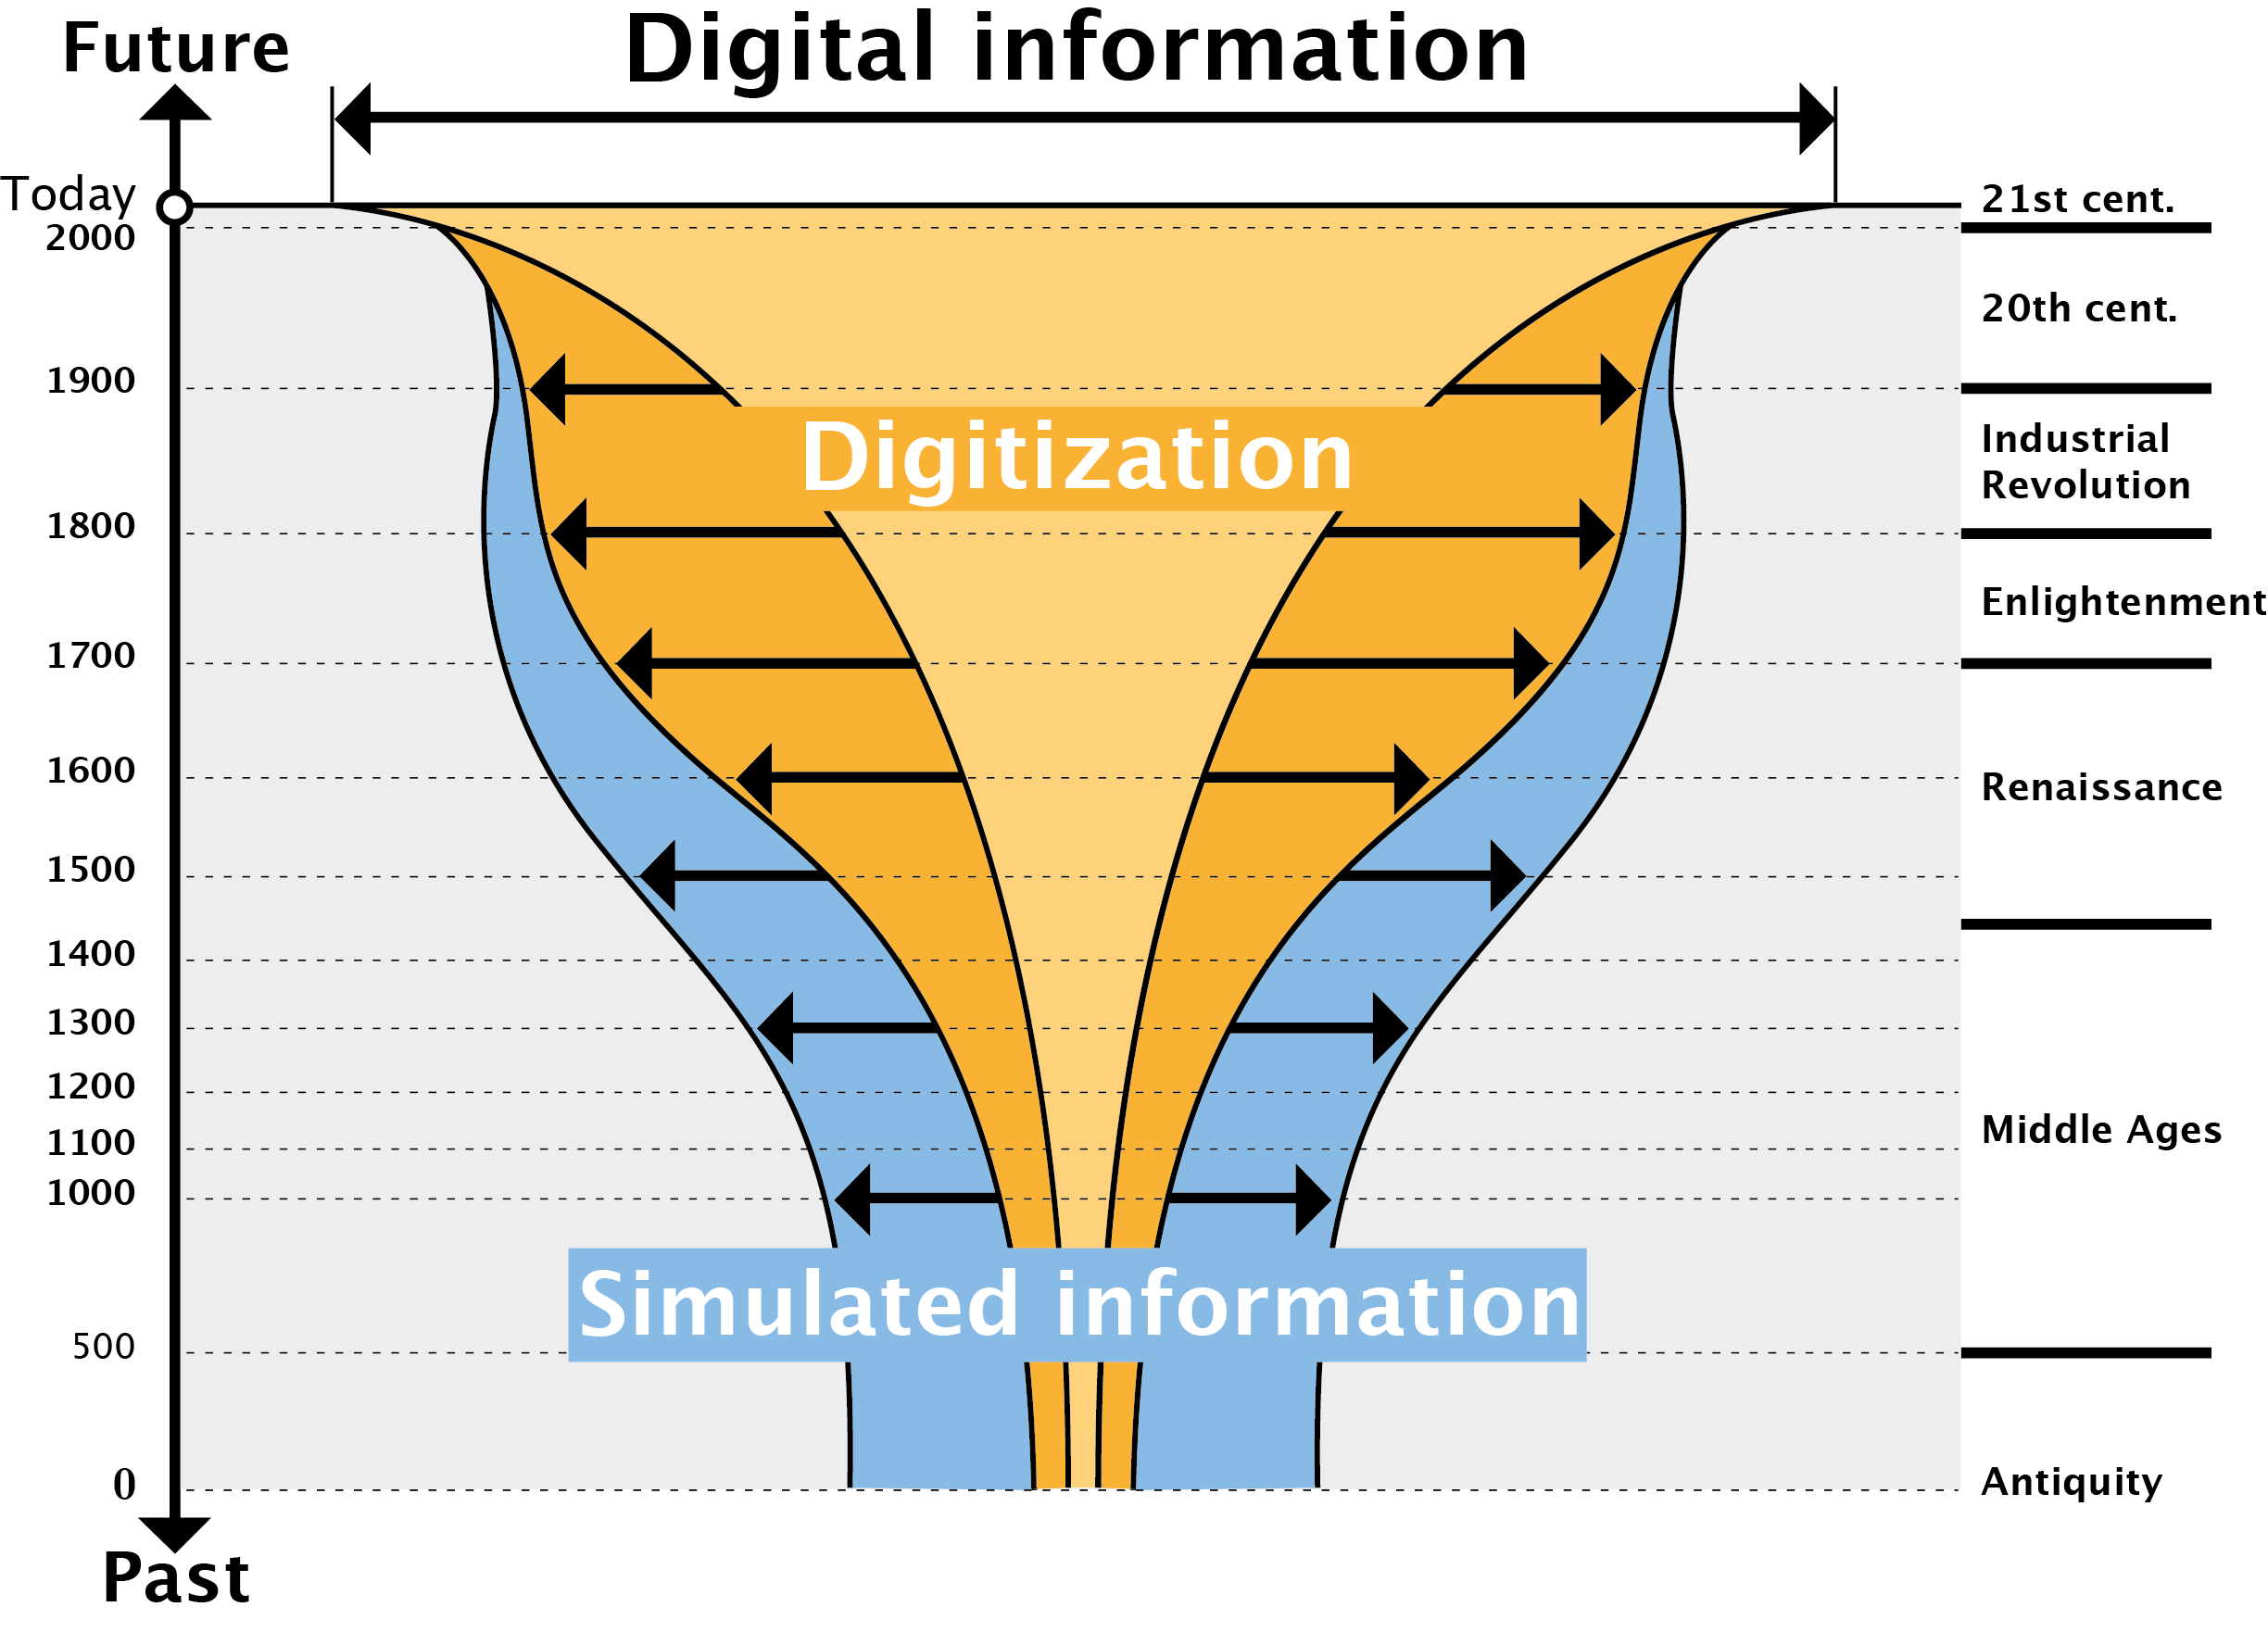
\includegraphics[width=\linewidth]{champignonKaplan.png}
 \legend{Legendary table}
  \end{sidecaption}
\end{figure}

Mais ce serait une erreur que de limiter l'application de ces nouveaux outils aux seuls stockages numériques récents, et ne pas citer l'importance du volume de connaissances accumulées ces derniers siècles par certaines sciences sociales telles que l'archéologie ou encore la géographie. Les lacunes dans l'information sont depuis longtemps une problématique récurrente pour de nombreuses disciplines en Sciences Humaines et Sociales. L'outil computationnel a permis dès lors qu'il a été disponible d'envisager de combler ces lacunes efficacement. Voir la figure ci dessous \ref{fig:I_Champi} \footnote{Voir l'article sur son blog \href{http://fkaplan.wordpress.com/2013/03/14/lancement-de-la-venice-time-machine/}{@FrédéricKaplan}}

%\begin{figure}[tb]
%\raggedright
%\begin{sidecaption}{This is a subcaption just for illustration purposes. This is a subcaption just for illustration purposes. 
%Champignon Informationnel de Frédéric Kaplan. Page number is \LARGE\textbf{\thepage}}[fig:test]
%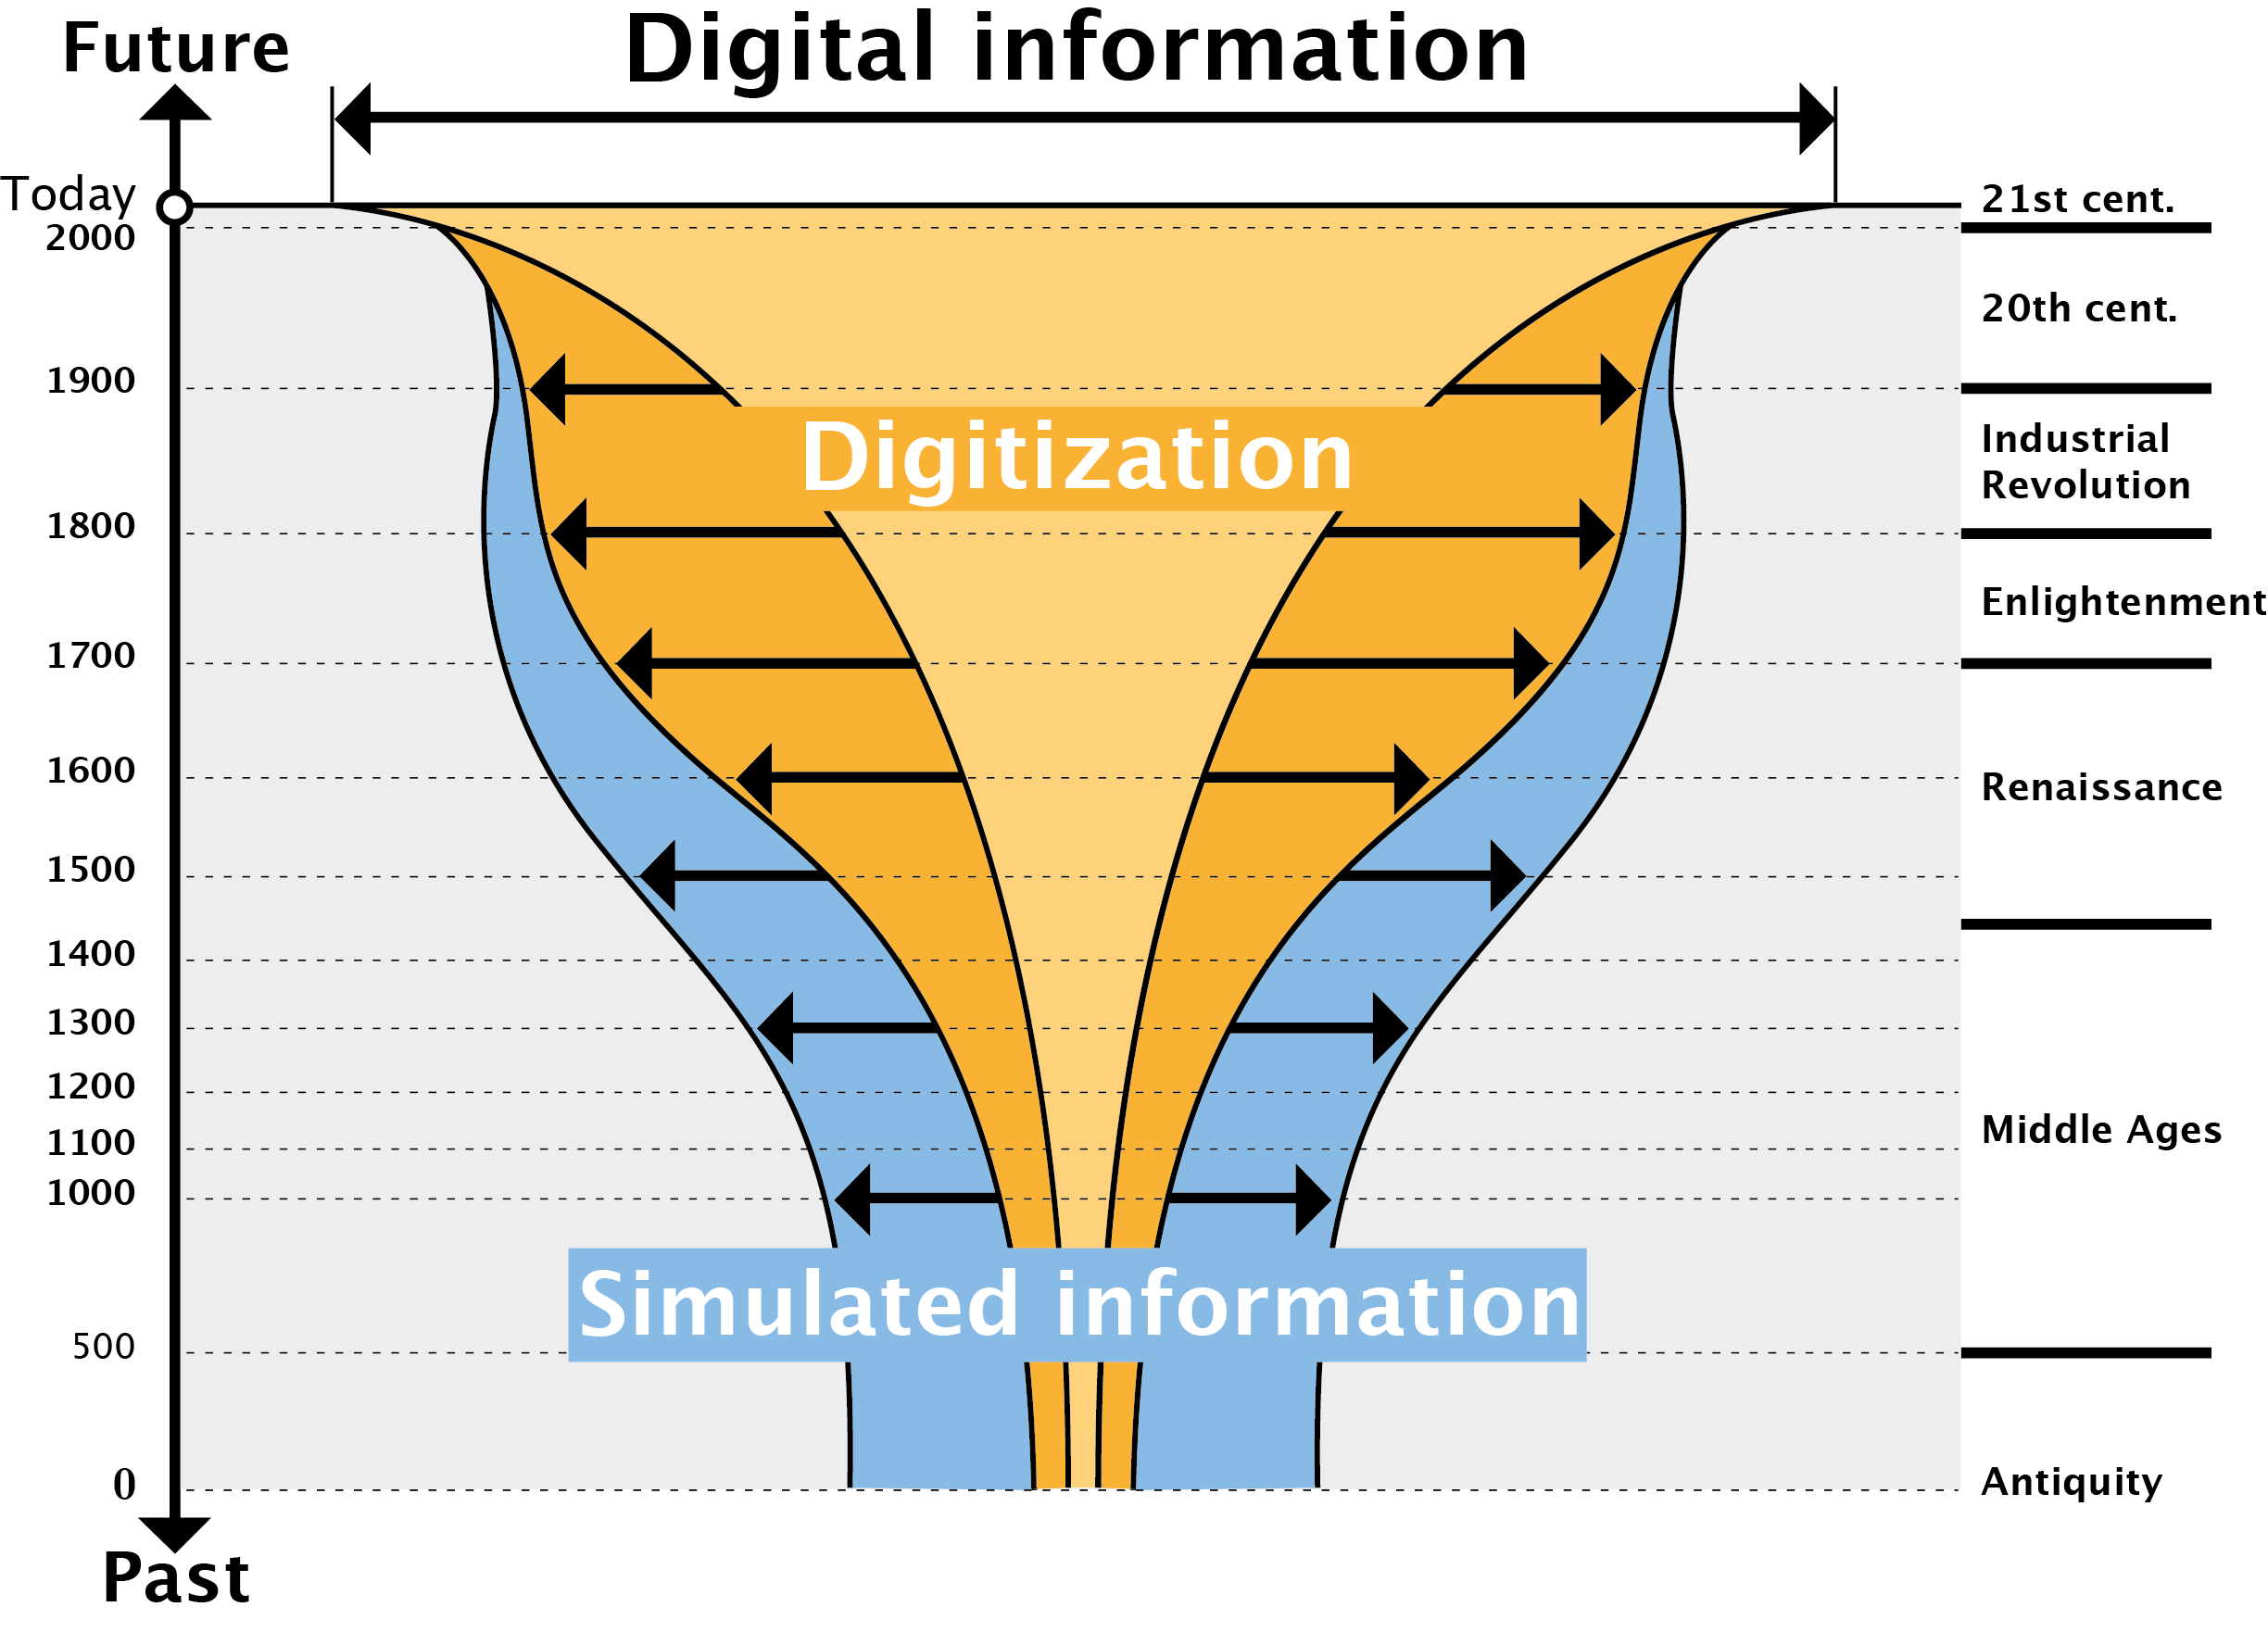
\includegraphics[width=\linewidth]{champignonKaplan.png}
%\end{sidecaption}
%\end{figure}

La classification automatique des données par l'ordinateur mais aussi la construction de modèles et leur simulation (au sens d'abord mathématique et parfois algorithmique du terme) apparaît rapidement comme un enjeu pour la géographie. La simulation apparaît comme un outil de construction de connaissance absolument naturel et nécessaire pour confronter et construire les théories en rapport avec ces données \autocite{Kao1963, Hagerstrand1967b}. L'image de cette communauté inter-disciplinaire agitant et confrontant ses problématiques méthodologiques, techniques, théoriques dans un but de progression commun, fait écho à des revendications plus récentes \footnote{On pensera notamment à la communauté ABM inter-disciplinaire qui gravite autour de la revue JASSS fondée en  1990}. En réalité cet esprit de partage tient d'une \enquote{volonté commune} qui apparaît quasiment avec l'apparition et la démocratisation des techniques de simulation. C'est ainsi que l'on trouve trace des efforts de cette communauté de chercheurs dans plusieurs ouvrages tels que \autocite{Beshers1965,Naylor1966,Dutton1971,Guetzkow1962,Guetzkow1972}.

Une citation d'un météorologiste du MIT, tout à fait remarquable par sa lucidité, anticipe ce qui sera le principal argument de l'emploi de la simulation en sciences humaines, à savoir un substitut à l'expérimentation \foreignquote{english}{I have argued that in the near future the social science will remain largely empirical and that simulation can serve as a device for making experiments \textbf{in vitro}. I think that this use is more important, at this time, than the massive making of models and that the principal contribution of simulation lies in the direction of intelligent, vivacious empiricism} \autocite{Fleisher1965}

%Forrester1969 à ce sujet "In the social sciences failure to understand systems is often blamed on inadequate data... The barrier is deficiency in the existing theory of structure." \autocite[355]{Batty1976}

\subsection{Les conditions d'apparition de la simulation dans les différentes sciences sociales }
\label{sec:apparition_simu_science_sociales}

\subsubsection{Bref rappel autour des définitions de modèles et de simulations}
\label{ssec:rapell_termes_generiques}

Nous apportons ici une petite digression afin de préciser quelle acception de la simulation nous souhaitons mettre en oeuvre dans notre thèse.

\paragraph{Définitions générales du terme \enquote{modèle}}

\textcite{Varenne2013} ont entrepris une classification de la richesse historique associée aux termes de modèle et de simulation.

La première définition généraliste et aussi la plus couramment encore rencontrée dans la littérature est probablement celle de Marvin Minsky établie en 1965 \autocite{Varenne2008} \autocite[15]{Varenne2013}  : \enquote{ Pour un observateur B, un objet A* est un modèle d’un objet A, dans la mesure où B peut utiliser A* pour répondre à des questions qui l’intéressent au sujet de A } \autocite{Minsky1965}

A partir de cette définition très formelle, Franck Varenne \autocite{Varenne2008} relève dans une analyse plus moderne du terme les cinq points suivants : 
\begin{enumerate}
  \item Le modèle n'est pas nécessairement une représentation
  \item Le modèle doit son existence à l'existence d'un observateur subjectif, et d'un questionnement lui aussi subjectif
  \item Le modèle est un objet qui a une vie propre, une existence autonome
  \item L'existence du modèle est justifiée par l'existence d'une \enquote{fonction de facilitation}
  \item Cette caractérisation minimale permet l'établissement d'une typologie
\end{enumerate}

Franck Varenne propose dans des travaux plus récents \autocite{Varenne2013} d'associer à cette définition les travaux de Mary S. Morgan et Margaret Morrison qui replacent et caractérisent le rôle du modèle dans une enquête de connaissance par sa fonction de médiation (point 4 de la liste), une façon de faire écho à la problématique motivant la construction de modèles établie dans la définition de Minsky.

Un modèle est ainsi défini comme \enquote{un objet médiateur qui a pour fonction de faciliter une opération cognitive dans le cadre d'un questionnement orienté}, opération cognitive qui peut être de cognition pratique (manipulation, savoir-faire, apprentissage de gestes, de techniques, de conduites, etc.) ou théorique (récolte de données, formulation d'hypothèses, hypothèses de mécanismes théoriques, etc.) \autocite{Varenne2013}

Les travaux actuels de \textcite{Varenne2008, Varenne2013} dénombrent pas moins de cinq familles pour un total de vingt grandes fonctions, ce qui permet de situer efficacement la ou les problématiques - rien n’empêche les fonctions de se recouper - qui motivent la construction d'un modèle. 

Nous verrons dans la section \ref{ssec:revol_modele} que les géographes modélisateurs ont mis dans leur définition davantage l'accent sur le rôle et les résultats attendus des modèles, plutôt que sur ces aspects formels.

\paragraph{Définition générale du terme \enquote{simulation}}

Le terme \enquote{simulation}, tout comme le terme \enquote{modèle}, est porteur d'une polysémie qui remonte aux alentours de l'accélération de sa diffusion en 1960 \footnote{ \textcite[343-350]{Morgan2004} propose une analyse intéressante de la diversité d’acception pouvant sous tendre l'emploi du terme \enquote{simulation} en se basant sur l'état de l'art réalisé par \textcite{Shubik1960a} en 1960, mais on peut aussi citer des sources plus directes comme les rapports fait par les instituts scientifiques militaires proche de l'OR : \foreignquote{english}{ The term \enquote{simulation} has recently become very popular, and probably somewhat overworked. There are many and sundry definitions of simulation, and a review and study of some of these should help in gaining a better perspective of the broad spectrum of simulation.} \autocite{Harman1961}}, mais nous retenons ici simplement les acceptions qui concernent la simulation computationnelle.

Bien que la simulation apparaisse sous sa première forme computationnelle dans la technique de Monte-Carlo et les travaux de Von Neumann et Ulman \autocite{Eckhardt1987}, il faut attendre les années 1960 et les avancées techniques nécessaires pour que son utilisation semble utile. L'historienne en économie \textcite{Morgan2004} estime que le mot se diffuse vraiment dans la communauté inter-disciplinaire, et en économie, aux alentours de 1960. Elle souligne le rôle central de Martin Shubik, un des pères de la théorie des jeux \footnote{voir sa \href{http://blogs.library.duke.edu/rubenstein/2012/12/18/the-martin-shubik-papers-from-early-game-theory-to-the-strategic-analysis-of-war/}{@Biographie}} dans la construction de ce débat autour de la notion \footnote{Shubick est aussi présent à un des tout premiers symposiums sur le sujet organisés par \textit{American Economic Review} \autocite{Shubik1960b}, où il retrouve d'autres pionniers de son époque, comme \textcite{Orcutt1960}, et Clarkson aidé de Simon \autocite{Clarkson1960}}, comme celui qui a servi à la fois d'intermédiaire important dans la rencontre entre les différents acteurs de l'économie expérimentale et de l'informatique, mais aussi comme celui tout aussi important de prospecteur au travers des vastes études bibliographiques qu'il a réalisées sur le sujet \autocite{Shubik1960a, Shubik1972} \autocite{Morgan2004}.

Par la suite d'autres conférences et ouvrages vont proposer de délimiter, toujours dans une construction inter-disciplinaire, cet objet \enquote{simulation}, comme on peut le voir dans \autocite{Guetzkow1962, Borko1962, Guetzkow1972, Dutton1971}. La simulation computationnelle est rapidement reconnue par les disciplines en sciences sociales ou les sciences du comportement comme un outil important pour la construction et l'extension de théories (\textit{theory-building} ou \textit{model-building} selon la fonction définie pour le modèle), de par sa capacité à manipuler certes des symboles mathématiques, mais aussi des symboles de plus haut niveau d'abstraction, propre à l'établissement de règle \autocite[924-925]{Clarkson1960}. Dans notre étude les modèles de simulation seront évoqués dans leur dimensions avant tout numérique ou algorithmique (cf. dirigés par des règles) \autocite[36-38]{Varenne2013}.

\subsubsection{La simulation vue comme laboratoire virtuel d'expérimentation, une analogie ancienne}
\label{ssec:labo_virtuelle}

Parmi la vingtaine de fonctions épistémiques recensées par \textcite[14-23]{Varenne2013} motivant la construction de modèles de simulation, la caractéristique la plus souvent exprimée pour l'époque en sciences sociales est sûrement cette capacité à pouvoir \enquote{expérimenter} sur les modèles en mobilisant des processus et des interactions sélectionnés et animés dans le cadre d'une dynamique, d'un temps mimant celui des systèmes cibles \footnote{Plusieurs auteurs, comme \autocite[462]{Gullahorn1965}, \autocite[296]{Doran1970}, \autocite[294-295]{Batty1976} semblent faire référence implicite ou explicite à cette action de \enquote{plonger le modèle dans le temps}. Hors \autocite[31]{Varenne2013} indique que cette dénotation se rapporte principalement au temps du système cible, et non pas au temps du modèle, qui peut être simulé autrement (en usant par exemple d'un tirage probabiliste). Cette référence n'est donc pas un marqueur permettant de caractériser en elle-même la notion de \enquote{simulation de modèle}}, et cela même dans des conditions difficiles caractérisées par l'absence ou l'inconsistance des données, les expérimentations réelles impossibles ou difficiles, etc. mais pas seulement, car la simulation de modèles a aussi vocation à simplifier certaines simulations physiques coûteuses, ou trop limitées dans l'expression de nouvelles hypothèses. Ce lien entre simulation et expérimentation, complexe du fait de la relation entretenue entre le modèle et la réalité, est aussi ancien que la technique elle-même, Von Neumann affirmant dès le départ sa volonté de remplacer par des simulations sur ordinateur certaines techniques coûteuses de simulation physique \autocite[15]{Winsberg2013}.

\Anotecontent{laboVirtuel}{Les récentes et au moins tout aussi récurrentes critiques sur l'apport d'une telle expérimentation dans les sciences sociales montrent qu'il est intéressant de développer quels sont véritablement ces points de similitudes et de divergences entre l'expérimentation physique et virtuelle, ne serait ce que pour construire une argumentation lisible à destination des nouveaux modélisateurs. Des sociologues des sciences comme Bruno Latour ou Ian Hacking ont développé ces vingt dernières années une véritable épistémologie des pratiques de laboratoire centrées autour de la démarche expérimentale, des réflexions qu'il nous faut prendre absolument prendre en compte pour toute analyse qui se voudrait plus poussée sur cette notion, comme en témoignent les travaux récents des épistémologues spécialisé dans la simulation comme Winsberg, ou \textcite[204]{Varenne2012}}

Régulièrement employée dans la littérature, cette fonction d’expérimentation revient également sous la forme de \enquote{laboratoire virtuel}, un terme qui prend selon les époques des teintes légèrement différentes, et cela quelles que soient les techniques sous-jacentes de support à la simulation des modèles.\Anote{laboVirtuel}

Cette analogie ancienne entre simulation et laboratoire virtuel est illustrative d'une réalité dont on aurait bien du mal à nier l'existence tant celle ci est persistante dans cette littérature. Parfois le terme est invoqué directement, parfois il est implicite au discours présenté. Pour ne citer que quelques auteurs pionniers dans l'historique de la notion, les premier ouvrages collectifs en simulation et science sociale de \textcite{Borko1962, Guetzkow1962, Guetzkow1972}; les rapports et états de l'art des instituts scientifiques militaires américains \autocite{Harman1961}, \footnote{La légende veut que l'idée d'appliquer la simulation aux \textit{Behavioral Science} viendrait d'un déjeuner entre Guetzkow et des physiciens nucléaire lors de son séjour au Carnegie, pour en savoir plus : \href{http://www.hawaii.edu/intlrel/pols635f/Guetzkow/hg.html}{@Harold} } \footnote{L'ouvrage de 1962, difficile à trouver, contient des re-publications de publications inédites dans plusieurs disciplines : Orcutt en économie \foreignquote{english}{Simulation of economic systems}, Coleman en sociologie \foreignquote{english}{Analysis of social structures and simulation of social processes with electronic computers}, Abelson en psychologie et science politique \foreignquote{english}{Simulmatics project}, Hovland en psychologie sociale avec \foreignquote{english}{Computer simulation of thinking} } et les travaux de Herbert Simon et Alan Newell \autocite{Newell1961}; et de façon plus localisé, en économie \textcite[915]{Shubik1960b}, en psychologie sociale \textcite{Abelson1968} \footnote{Un auteur connu aussi pour avoir échangé aussi avec \textcite{Boudon1967} sur la simulation à la même période, voir  \textcite{Padioleau1969}}, \textcite{Fleisher1965} météorologue, le couple d'Anthropologues/sociologues du comportement \textcite{Gullahorn1965}, l'archéologue anthropologue et informaticien \textcite{Doran1970}, la physicienne biostatisticienne et démographe \textcite{Sheps1971}, l'informaticien \textcite[3-4]{Forrester1971}, l'économiste informaticien \textcite{Naylor1966}, le professeur de science régionale \textcite[271]{Harris1966}, l'urbaniste \textcite[295]{Batty1976} sans oublier plus récemment \textcite{Epstein1996}, l'écologue \textcite{Grimm2006}, et encore sûrement bien d'autres auteurs. Une longue liste qui témoigne de l'intérêt pour cet outil bien au delà d'un simple critère de démarcation disciplinaire, technique, ou encore temporel; une hypothèse que nous allons développer par la suite.

\subsubsection{Un engouement pour la simulation qui touche l'ensemble des sciences sociales}
\label{ssec:engouement_sciencesociale}

Cet engouement pour la simulation de modèles touche toute les sciences sociales ou presque. Nous dressons dans les paragraphes qui suivent une brève énumération des travaux qui en témoignent pour la période 1950-1970.

Suite au mouvement Cybernétique, à la convergence des travaux sur l'intelligence artificielle et les sciences cognitives, les premiers travaux qui visent la démonstration de la faisabilité de la simulation dans les sciences sociales viennent de Newell, Shaw, et Simon à la fin des années 1950 \autocite{Gullahorn1965} \footnote{Avec plusieurs tentatives pour la construction d'une machine universelle de résolution de problème (\foreignquote{english}{Logic Theorist program} en 1957 et \foreignquote{english}{General Problem Solver} en 1959). Ce programme s'avère également être la première pierre posée de l'intelligence artificielle, en formation à l'intersection de la naissance encore récente des sciences cognitives et de l'informatique. Cette machine est conçue pour mimer les capacités de résolution de l'esprit humain, et permet enfin d'exprimer et de questionner les théories comportementales dans un langage informatique alors plus précis et moins ambigu que le langage naturel. Le programme est ainsi capable de résoudre des problèmes aussi différents que de jouer aux échecs, de résoudre des problèmes mathématiques, ou de retrouver des motifs dans des données.} A ces travaux s'ajoutent ceux, en psychologie linguistique de l'équipe gravitant autour de \textcite[280-416]{Borko1962}, en psychologie des comportements sociaux de \textcite{Hovland1960}, d'\textcite{Abelson1961, Abelson1968} ou du couple \autocite{Gullahorn1965a} qui utilisent la simulation de modèle pour formuler, vérifier des théories sur la psychologie des individus et les modalités de leurs interactions avec les autres dans diverses situations \footnote{Les applications sont menées à des échelles très diverses, ainsi alors que le modèle Homonculus développé par le couple Gullahorn tente de mieux comprendre les stratégies de résolution de conflits avec la programmation de comportements au niveau individuel \autocite{Gullahorn1965}, le projet \textit{Simulmatics} mené par \textcite{Abelson1961} vise quand à lui l'étude du comportement de groupes d'électeurs en cas de conflit d'opinion (ou \foreignquote{cross-pressure}) pour tenter en fonction d'un échantillon de population d'analyser l'impact de stratégies politiques, une demande de J.F.Kennedy pour la campagne de 1960 aux États-Unis}, ce que \textcite{Ostrom1988} appellera \foreignquote{latin}{a posteriori} les \foreignquote{english}{complex human processes}.

%La formation d’ingénieur de Coleman l’amène à prendre comme modèle un physicien : « My real hero is not Isaac Newton, but James Clerk Maxwell. He took Newtonian theory and developped from it a theory of gases, the Maxwell-Boltzmann distribution law of molecular velocities. I was fascinated by Maxwell because he was also concerned with the micro-macro problem. He had a very simple and neat theoretical framework of dimensionless molecules of any gas acting according to the law of motion, each with a certain mass and velocity. And from this he constructed a theory of gas. » (Coleman dans Swedberg, 1990, pp. 55-56).

En \textbf{sociologie}, la simulation émerge dans les années 1960-1970 selon \textcite[50]{Manzo2005}, sous l'impulsion de pionniers dans la sociologie mathématique comme \textcite{Boudon1967} en France \footnote{Selon \textcite[61]{Manzo2005}, Boudon a très tôt supporter l'idée des modèles de simulation comme support à l'explication, comme il témoigne à propos de ces écrits des années 60-80 : \enquote{À ce moment, j’avais publié divers écrits sur l’individualisme méthodologique, la théorie de l’action, la rationalité et les \enquote{modèles générateurs}. Mes travaux sur l’éducation m’avaient en effet convaincu que ni l’analyse multivariée ni les méthodes statistiques d’\enquote{analyse des données} ne permettaient d’expliquer les régularités statistiques qui sont le pain quotidien du sociologue : il fallait tenter plutôt de les engendrer à partir d’hypothèses sur les logiques de comportement des acteurs.} \autocite[391]{Boudon2003}}, ou James Samuel Coleman aux Etats-Unis \footnote{C'est à l'université de Columbia sous la direction du sociologue Robert Merton et du mathematicien-sociologue Paul Lazarsfeld, des acteurs influents dans l'application des méthodes quantitatives à la sociologie \autocite{Lazarsfeld1954} aux États-Unis mais également en France (il collabore avec Boudon sur plusieurs projets, d'enseignements et de publications) et à l'international \autocite{Lecuyer2002}, que James Coleman publie en 1964 \textit{Introduction to Mathematical Sociology} \autocite{Coleman1964}, un ouvrage devenu une référence en sociologie quantitative dont on peut lire un résumé élogieux dans la \textit{Revue francaise de Sociologie} réalisé par \textcite{Boudon1966} en 1966.} et de simulation, celui-ci considérant cette dernière {[...] as a half-way point between verbal speculative theory and formal theory, aiding in the development of such theory through concretizing the functioning of \foreignquote{english}{social processes}. \autocite[36]{Guetzkow1972}}.

Celui-ci travaille sur des simulations liées à ses recherches sur l'éducation au début des années 1960 aux États-Unis, dont il a déjà publié des travaux dans l'ouvrage inter-disciplinaire de \textcite{Guetzkow1962} en 1962, et qu'il publie ensuite \autocite{Coleman1965} dans une des premières revues abordant la méthode de simulation en sociologie, un numéro spécial des \textit{Archives Européennes de Sociologie} introduit par \textcite{Boudon1965} en 1965. Dans ce  numéro figure également une des premières traductions de la simulation de diffusion d'Hägerstrand \autocite{Hagerstrand1965} utilisant la technique de Monte-Carlo, un modèle qui recoupe les préoccupations du vaste courant inter-disciplinaire dit des SNA (Social Network Analysis) \autocite{Bernard2005}, qui touche tout autant aux structures de parenté (voir le paragraphe suivant pour des références en Anthropologie), qu'à la géographie (Hägerstrand à Lünd), ou à la sociométrie (modèle du sociologue mathématicien Coleman \textcite{Coleman1957}, mais également modèle de \textcite{Rapoport1961}, un biomathématicien de Chicago et confondateur avec Boulding, Gerard et Von Bertalanffy de la société pour l'étude des systèmes généraux, ou GST) \footnote{Une analyse croisée entre des modèles de différentes disciplines sur la diffusion des innovations, contenant notamment les modèles d'Hägerstrand et de Rapoport a été publiée en 1968 dans la revue \textit{Lund Studies in Geography} par \textcite{Brown1968}}. Du point de vue français, outre l'analyse de Boudon sur ce sujet dans le numéro spécial de 1965, on trouve également une revue de ces mêmes avancées en simulation du côté de la sociologie politique (qui recoupe la psychologie sociale américaine), un état de l'art réalisé par \textcite{Padioleau1969} dans la \textit{Revue francaise de sociologie} en 1969.

\Anotecontent{archeo_stat}{Des transferts parfois étonnants en provenance d'autres disciplines, comme le montre cette citation : \foreignquote{english}{Similar trends are apparent in allied subjects such as anthropology and social geography. In particular, location analysis has influenced archaeologists, with its emphasis on the study of all aspects of a population and its environment, and on the use of quantitative methods and models (Haggett 1963)} \autocite{Doran1970}}

\Anotecontent{archeo_systemique}{Une analyse a posteriori confirme l'apport de la systémique dans la construction des modèles de simulation, comme en témoigne \textcite[5]{Lake2013} et de façon plus précoce \textcite{Aldenderfer1998} en 1988. \foreignquote{english}{One of the theoretical hallmarks of the \textit{New Archaeology} was the systems approach \autocite{Aldenderfer1991}, and a result of its adoption was the use of computer simulation to model whole societies or significant portions of them.}}

\Anotecontent{whallon_simulation}{\foreigntextquote{english}[Whallon1972, 38]{The techniques and procedures of computer simulation so closely parallel the current thinking and processes of model-building of many archaeologists that the lateness and limits of their application are surprising.}}

%% FIXME ORTHOGRAPHE
En archéologie, dans la très claire retrospective historique faite par Gary Lock en 2003\autocite{Lock2003} sur l'histoire de l'archéologie computationelle, l'auteur s'attache à bien séparer au moins deux sinon trois époques aux méthodologies et aux outils différents. En adoptant une posture un peu simplificatrice on peut donc affirmer que si l'archéologie pre-années 1960 se base principalement sur la récolte de données empiriques et la mise en exergue de pattern dans ces même données pour générer la plupart de ces explications, une rupture dans la discipline se dessine dès les années 1960-70 avec l'avénement d'un courant d'archéologie proclamant une \enquote{ new archeology} (ou \emph{processualism}). Rejettant un empirisme beaucoup trop subjectif, celle ci vante le retour à la seule \enquote{ Méthode Scientifique } pour générer des explications. 

\Anotecontent{wilcock_stat}{On trouve un récit plus détaillé de l'arrivée des méthodes statistiques en archéologie dans la publication de \autocite{Wilcock1997}}

\Anotecontent{caa}{Il est intéressant de noter que ces quelques archéologues pionniers en informatique ont très vite créés leur propres canaux de diffusion en angleterre. Si de multiples conférences pour le développement des aspects computationels en archéologie existent à la charnière 1960-1970 (Rome, New-York, Marseille) \autocite{Wilcock1997}, ce n'est qu'en 1973 que se forme sous le patronage de quelques chercheurs anglais la première \foreignquote{english}{Computer Applications and Quantitative Methods in Archaeology Conference} \href{http://caaconference.org/about/}{@CAA}. Celle-ci se tient sa première édition à Birmingham, et deviendra par la suite en 1992 une conférence à portée internationale. La particularité de cette conférence, qui existe toujours, est son inter-disciplinarité; le comité d'organisation militant toujours pour la rencontre et le dialogue entre  archéologues, mathématiciens et informaticiens. A l'ocasion des 40 ans de la conférence en 2012, le projet \foreignquote{english}{Personnal-Histories Project} à permis la collecte et la mise à disposition de témoignages vidéo des pionniers sur le site de \href{http://www.sms.cam.ac.uk/collection/750864}{@Cambridge}}

Si la critique de 1962 opéré par \textcite{Binford1962} cristalise pour beaucoup cette rupture, 1968 est également considéré comme une année particulièrement importante pour la structuration de ce courant dans la discipline. L'avénement de plusieurs publications phares vient souligner l'émergence progressive dans les années 1960-70 de nouveaux outils \Anote{caa}, à la fois computationels comme les statistiques \Anote{wilcock_stat} ou la simulation \autocite{Clarke1968} , ou plus conceptuels avec l'ancrage de la \foreignquote{english}{New Archeology} dans la pensée systémique \autocites{Clarke1968, Flannery1968, Binford1968} \Anote{archeo_systemique}. Des avancées qui fournissent un véritable support à ce changement des pratiques dans la discipline.

\Anotecontent{doran_intuition}{\foreignquote{english}{There has now been a wide variety of experiments involving computer processing of archaeological data. Clarke (1968) describes many of them, and another valuable source is Cowgill (1967). I do not propose to discuss these experiments here, important though they are. [...] In this final section I shall briefly present the computer in what seems to me to be a much more promising and interesting role, which has as yet received rather little attention from archaeologists, even though in some ways it can be regarded as the practical equivalent of systems theory. I mean the use of a computer to construct and test a \enquote{simulation} of some complex system evolving in time. [...] Indeed, one of the great advantages of using a computer program to simulate evolving systems is that a much wider range of possibilities can be accommodated than can be expressed mathematically.} \autocite{Doran1970}}

Si \textcite{Binford1968} représente le point de vue américain, Clarke présente en angleterre et à la même période (\textcite{Clarke1968} est édité en 1968 par Binford) un point de vue un peu différent sur la New-Archeology \autocite{Binford1983}. Clarke est en effet sous l'influence des idées animant le campus de Cambridge, un haut lieu de changement ayant déjà accueilli une autre révolution, celle de la \textit{New-Geography} \Anote{archeo_stat}. C'est dans cet environnement que Clarke publie en 1968 un premier livre \foreignquote{english}{Analytical Archeology} qui démontre le potentiel que pourrait avoir les statistiques spatiales, les modèles et la simulation stochastique en archéologie \autocites{Clarke1968, Clarke1972} (ce dernier meurt jeune en 1976). Il est accompagné dans ses travaux par l'expertise, la volonté et les intuitions pionnières \Anote{doran_intuition} de James Doran \autocite{Doran1970} qui écrit également avec Hodson en 1975 l'ouvrage devenu référence \foreignquote{english}{Mathematics and Computers in Archaeology} \autocite{Doran1975} faisant état des travaux utilisant les toutes dernières techniques computationelles à la fois en traitement de données, et en simulation (Chaîne de Markov, Monte-Carlo, langage pour la simulation Dynamo, GPSS, etc.)

Ce militantisme qui semble recevoir un écho positif tout au long des années 1970 \footnote{On pourra trouver plus d'informations sur les premiers travaux dans les ouvrages cités précédemments, et via des retrospéctive plus récente comme celle de \autocite{Kohler2011}, ou \autocite{Lake2013}}, certains auteurs comme \textcite[38]{Whallon1972} n'hésitant pas à définir\Anote{whallon_simulation} la simulation comme un prolongement naturel à la pratique existante de construction des modèles. Cette mise en oeuvre de programmes pionniers se poursuit avec une diversification dans les usages jusqu'au début des années 80 et constitue une première phase d'appréhension de la simulation, plus qu'une adoption massive par la discipline. \autocite{Lake2013}

% VOir aussi Mathematics and Computers in Archaeology doran 1975, partie sur la simulation cf http://books.google.fr/books?id=ZAPvXcnz0kkC&pg=PA369&lpg=PA369&dq=The+computer+in+archaeology:+A+critical+survey+whallon&source=bl&ots=6et-F8jHab&sig=gQWgTIHRuO2ICqMJtrRdGovo9gs&hl=fr&sa=X&ei=OskxU5W5Nen20gW0_4DIDA&ved=0CGUQ6AEwBQ#v=onepage&q=whallon&f=false

%\autocite{Clarke1987}

A la croisée de plusieurs disciplines, sociologie, anthropologie et géographie on trouve les modèles de variation de population, ou modèles démographiques dont les hypothèses sont amenées à varier selon des facteurs biologiques, économiques, spatiaux faisant souvent appel à une dynamique des interactions humaines impossible à expérimenter dans la réalité. \footnote {\foreignquote{english}{To understand how changes in the size and composition of human populations occur, it is essential to study the determinants of these changes and the interrelations among them. The impossibility of investigating these relationships experimentally stimulates the formulation of models, as a means of enhancing our understanding of the process.} \autocite{Sheps1971}} Dans cette branche se côtoient donc macro-simulation, micro-simulation et modèle analytique hérités des premiers démographes mathématiciens, comme le plus connu d'entre eux, Lotka dont les premières publications sur le sujet datent de 1907 \autocite[355]{Veron2009}.

%%FIXE CLEMENTINE : c’est intéressant, que la plupart des travaux pionniers que tu cites  apparaissent dans les urban studies.  Est-ce que c’est la ville qui est si complexe ou une dépendance au chemin des méthodes dans les champs d’études ? ou parce que urban studies est particulièrement interdisciplianaire que ça a dépasser les barrières des affiliations disciplinaires ?

Les modèles TRIM, puis DYNASIM (entre 69 et 75) développés par Orcutt et son équipe à l'\foreignquote{english}{Urban Institute} sont pionniers \autocite{Orcutt1957, Orcutt1960, Orcutt1976}, et inspirent différents modèles dynamiques en démographie avec les travaux de \textcite{Perrin1964}, \textcite{Sheps1971}, et \textcite{Ridley1966} avec REPSIM aux États-Unis,  \textcite{Hyrenius1964} en Suède, \textcite{Horvitz1971} avec POPSIM, ou encore SOCSIM basé sur les travaux en anthropologie de \textcite{Gilbert1966}, qui viennent compléter efficacement les modèles analytiques inspirés des travaux de Lotka \autocite{Sheps1971}, père entre autre de la démographie mathématique moderne. Coïncidence de l'histoire, ou inspiration commune, Hägerstrand apportera de façon parallèle en géographie, et dans la même décennie \autocite{Hagerstrand1952, Hagerstrand1967}, une vision micro similaire, à cela près qu'elle y ajoute un ancrage spatial des individus.

Dans le cas de l'anthropologie, qui partage un tronc commun avec nombre de problématiques en archéologie, et en psychologie, on retiendra le manuel édité par \textcite{Hymes1965} retranscrivant une conférence de 1962. Celui-ci contient deux articles importants pour la discipline, celui de \textcite{Gullahorn1965} et celui complémentaire de \textcite{Hays1965}. L'intégration de la simulation dans l'arsenal méthodologique prend part selon \textcite[274]{Bentley2009} d'un mouvement ayant pour objectif de mieux comprendre les contraintes sociales et culturelles dans les processus démographiques en général. Dans ce cadre par exemple de l'étude de la parenté ou \foreignquote{english}{kinship}, l'application de la simulation donne lieu à plusieurs expériences pionnières \autocite{Dyke1981} en simulation comme celle de \textcite{Kunstadter1963}, mais aussi de \textcite{Gilbert1966}. Cet engouement continuera dans les années 1970 \autocite{Read1999} avec des simulations mettant en œuvre des processus stochastiques dynamiques comme par exemple dans les travaux de \textcite{Howell1978} et \textcite{Thomas1973}.

%\autocite{Costopoulos2007} . %Antony Wallace également, levy strauss 1955: les mathématiques de l'homme...

%En utilisant la simulation non pas comme un solveur d'équation mais en utilisant la puissance des opérateurs symboliques à sa disposition pour la mise en temporalités de systèmes d'interaction dans des sociétés passées, Doran décrit une vision de la simulation qui n'est pas sans rapeller le multi-agent d'aujourd'hui. Une conception de la simulation reprise et concrétisée par DH Thomas en 1972.\footnote{La discussion sur  \href{www.jiscmail.ac.uk/cgi-bin/webadmin?A2=ind04\&L=simsoc\&F=\&S=\&P=39083} {@SimSOC}} 


% http://books.google.fr/books?id=G8sA95bz5pwC&pg=PA143&lpg=PA143&dq=%22Social+Physics%22+stewart+cybernetics&source=bl&ots=FsOC2mqHvr&sig=cS914G7pelGvgG6bG32fKsmWWPc&hl=fr&sa=X&ei=yTRAU5m7OIOH0AXwtYEY&ved=0CDsQ6AEwAQ#v=onepage&q=%22Social%20Physics%22%20stewart%20cybernetics&f=false
% "Social Physics" stewart cybernetics
% http://www.eoht.info/page/Princeton+Department+of+Social+Physics
% http://books.google.fr/books?id=F84mS2nnjWsC&pg=PA105&lpg=PA105&dq=geographer+reino+ajo&source=bl&ots=buVSBElr7Y&sig=_NXU0Py2goM2c6fVi1To3dUwqHQ&hl=fr&sa=X&ei=0DBAU_niJqrO0AWk44CwCw&ved=0CG8Q6AEwBw#v=onepage&q=geographer%20reino%20ajo&f=false
% http://www.persee.fr/web/revues/home/prescript/article/ingeo_0020-0093_1957_num_21_5_6491_t1_0223_0000_5#
% http://www.eoht.info/page/Social+physics
% Contributions to "social Physics" reino ajo
% Stewart, J.Q. "The Development of Social Physics"

\subsection{Les premiers modèles de simulation en géographie}
\label{sec:premier_modele_geo}

\subsubsection{Une \enquote{révolution quantitative} au cœur de multiples convergences}
\label{ssec:revol_quanti}

L'apparition et la diffusion de ces techniques quantitatives n'est pas le résultat d'une convergence unique, mais bien d'une succession de moments dont la fréquence et l'étalement temporel est difficile à cerner et empêche sur ce sujet toute exhaustivité. 

On retiendra toutefois plusieurs grands facteurs, à la fois généraux, et d'autres plus spécifiques à la géographie, dont certains qui peuvent paraître étonnamment antinomiques. Une convergence qui s'illustre dans la richesse et la diversité des transformations qui touche la discipline géographique entre 1950 et 1970, un constat déjà établi par bien d'autres auteurs \autocite{Varenne2014}

%[28-29]Claval2003
%http://books.google.fr/books?id=s5xjIsejTjkC&pg=PA28&lpg=PA28&dq=h%C3%A4gerstrand+positivism&source=bl&ots=FrIMA95glO&sig=9Knqs1cLfJJefcc30qwsIMDzW-s&hl=fr&sa=X&ei=UMVDU86hJ-mS1AWPmIDoCw&ved=0CC4Q6AEwADgK#v=onepage&q=h%C3%A4gerstrand%20positivism&f=false

\paragraph{L'influence de l'école néo-positiviste}

Le néo-positivisme, néo-empirisme, positivisme logique selon les étiquettes, est un mouvement philosophique important, sinon peut être le plus important, entre les deux guerres. Ce cercle dont on trouve les premières traces dans les années 1908 à Vienne, est organisé autour de grands débats, dont la caractéristique est d'être fréquenté par un grand nombre d'intellectuels, issus de plusieurs disciplines. Tout au long de son évolution caractérisée par différentes phases (avec une apogée durant la troisième phase entre 1928-1934), de multiples courants d'opinions \textcite[126]{Ouelbani2006} vont être amenés à se côtoyer, du fait des débats internes, mais aussi des critiques extérieures au cercle. C'est donc à ce titre que \textcite[11]{Ouelbani2006}, préfère parler de \enquote{programme néo-positiviste} \footnote{Le programme de Carnap tient en quatre points selon Dahms, cités par \textcite{Ouelbani2006} : (i) la réduction de la philosophie à une théorie de la connaissance; (ii) la distinction des sciences, non plus en sciences de la nature et sciences humaines, mais en sciences empiriques et analytiques: (iii) le logicisme comme programme de réduction des sciences analytiques; (iv) le réductionnisme comme programme de réduction des sciences synthétiques ou empiriques.} plutôt que d'un réel courant unifié.

Inspirés des sciences naturelles, et plus particulièrement d'une observation des sciences physiques et mathématiques, les tenants du programme néo-positiviste sont motivés par l'unification des sciences, et pensent l'application d'un tel programme incontournable pour fonder des sciences sociales véritablement \enquote{scientifiques}. \textcite[1-20]{Ouelbani2006}

Les positivistes logiques ont ceci de particulier qu'ils raisonnent sur des démonstrations logiques encapsulant les énoncés observationnels décrits dans une logique formelle qu'ils veulent non ambiguë. Entre empirisme et logicisme, ce programme réductionniste \footnote{Voir la définition du programme donné par Carnap dans la note précédente.} fait porter toute la connaissance sur l'expérience; ce qui mène avec l'aide de l'analyse logique et mathématique à l'élimination de toute métaphysique, et de toute structure a priori (anti-kantien) dans la construction des énoncés d'observation. Ainsi l'inférence déductive se fait seulement sur des énoncés d'observations qui sont \foreignquote{latin}{a posteriori} tout à fait justifiables, et donc mobilisables dans celle-ci seulement si ils cohérents.

Ian Hacking \autocite{Hacking1983} a ,selon Orain \footnote{Voir les notes de \href{http://www.esprit-critique.net/article-12642840.html}{@cours}, dispensés sur le blog \enquote{esprit critique} de Olivier Orain} très bien saisi ce qui fait les axes communs \footnote{Le positivisme peut se définir par quelques idées forces. (1) L’importance accordée à la vérification (ou à une variante comme la falsification) : une proposition n’a de sens que si l’on peut, d’une quelconque manière, établir sa vérité ou sa fausseté. (2) La priorité accordée à l’observation : ce que nous pouvons voir, toucher ou sentir fournit, sauf pour les mathématiques, la matière ou le fondement le plus appréciable de la connaissance. (3) L’opposition à la cause : dans la nature, on ne trouve pas de causalité dépassant ou surpassant la constance avec laquelle des événements d’un certain type sont suivis par des événements d’un autre type. (4) Le rôle mineur joué par l’explication : expliquer peut contribuer à organiser des phénomènes mais le pourquoi reste sans réponse. On peut seulement remarquer que le phénomène se produit régulièrement de telle ou telle manière. (5) Opposition aux entités théoriques : les positivistes ont tendance à être non réalistes parce qu’ils limitent la réalité à ce qui est observable mais aussi parce qu’ils s’opposent à la causalité et se méfient des explications. Leur rejet de la causalité les fait douter de l’existence des électrons simplement parce que ces derniers ont une action causale. Ils soutiennent qu’il s’agit là seulement de régularités constantes entre phénomènes. (6) L’opposition à la métaphysique est finalement le dénominateur commun entre les points (1) à (5) ci-dessus. Propositions invérifiables, entités inobservables, causes, explications profondes, tout cela, dit le positiviste, est objet de métaphysique et doit être abandonné. \autocite[82]{Hacking1983}.} des différentes relectures du terme positivisme. Une parenté qui dans le cas du programme néo-positiviste est difficile à isoler tant l'acceptation par les proches (comme Popper) ou membres du programme (certain préféreront même le terme empirisme logique) est amené à varier, on pourra ainsi se référer à la classification proposée par Hacking pour en savoir plus sur ce sujet. \autocite[81-86]{Hacking1983}

L'apogée du groupe à Vienne est de courte durée, avec les pressions du régime nazi et l'annexion de l'Autriche, le groupe est dissous. De nombreux acteurs du mouvement sont alors contraints à l'exil, et nombreux sont ceux qui vont aux États-Unis. A ce moment-là, ce programme philosophique est alors quasiment inconnu des philosophes pragmatistes américains, mais paradoxalement c'est sur ce nouveau territoire qu'il va trouver un très bon accueil. 

C'est sur cette philosophie pragmatique depuis longtemps installée (Peirce, Dewey) que vient se greffer ce nouveau programme, jusqu'à finalement quasiment l'éclipser. Un transfert que l'on n'imagine pas totalement unilatéral, et il est presque évident que le discours originel viennois tire largement profit d'une philosophie pragmatiste compatible dans ses fondements \footnote{ Ainsi selon \textcite[149]{Ouelbani2006} Carnap aurait été rassuré en 1935, date de son arrivée aux Etats-Unis, \enquote{ [...] de trouver une ambiance philosophique différente,en ce sens que les jeunes philosophes étaient intéréssés par des méthodes scientifiques et logiques}}. C'est ce que \textcite[123]{Wilson1995} affirme en disant que les pragmatistes \foreignquote{english}{[...] had created the conditions in which logical positivism and other analytic philosophies could flourish and ultimately displace them as the dominant voice in mid-century philosophical debates} mais aussi les conditions de son dépassement \foreignquote{english}{Pragmatism, then, not only created the conditions in which logical positivism and analytic philosophy could flourish in the United States, it also contained the seeds of the postanalytic philosophies that have attempted to move beyond [...] }. Ce programme va se diffuser à la fois sur les bancs des universités, mais aussi via les grands instituts scientifiques après guerre qui font publicité de cette science \foreignquote{english}{mainstream}, organisée aux Etats-Unis autour de l'ordinateur. 

La RAND fait partie de ces instituts fondés après guerre, qui approche dès 1947 les sciences sociales \autocite{Rand106}, et n'hésitent pas à mettre en avant par la suite les stars de la philosophie positiviste de l'époque comme Reichenbach \autocite[384-385]{Barnes2011} .

\paragraph{L'apparition de mouvements inter-disciplinaires fédérateurs}

L'apparition de grands mouvements de convergence inter-disciplinaires et leur intérêt pour l'application de nouveaux concepts et techniques aux sciences sociales, dont certains prennent par la suite la forme de paradigme du fait de leur portée d'application : Cybernétique de Wiener, \textit{projet} de la \foreignquote{english}{General System Theory} de Bertalanffy \autocite[9]{Pouvreau2013} s'organise autour de grandes structures de recherches comme le MIT, la RAND, qui favorisent les collaborations par la mise en place d'équipe de travail pluri-disciplinaire.

Parmi les ramifications directes de ces coopérations, on citera par exemple la \enquote{social physics} de Stewart \autocite{Stewart1947}. Du fait des liens développés à l'université de Pennsylvanie, lieu de ses études, et siège de la fondation de la science régionale d'Isard en 1954, Stewart sera amené avec sa rencontre avec Warntz, un géographe atypique qui plonge très tôt dans l'inter-disciplinarité, à publier dans la revue \textit{Regional Sciences} \autocite{Stewart1958}.

Les retombées de ces interactions sur la géographie sont importantes \footnote{ A condition de ne pas oublier qu'une partie de ces concepts existent de façon sous-jacente aux disciplines, ce qui explique parfois leur rapidité d'acceptation. C'est le cas de l'approche systémique développée par la cybernétique quand elle ne fait pas qu'apposer un nom commun sur des concepts déjà étudiés, mais fait alors écho à des révolution méthodologiques en attente d'être activée. \textcite[5]{Batty1976} résume la situation ainsi \foreignquote{english}{The idea of systems being described in terms of structure and behaviour, in terms of input and output, and the notion of purposeful control of such systems in terms of negative and positive feedbacks, appeared to many social scientists an ideal description of their systems of interest and thus the approach has come to be used in more-or-less all of the social sciences}.}, et fournissent tout autant : (i) des concepts généraux en correspondances avec les débats qui animent l'ensemble des sciences : sensibilité aux conditions initiales, équifinalité, bifurcation et catastrophe, boîte noire, rétro-causalité, hiérarchie d'emboîtement, etc.) , (ii) un catalogue d'isomorphisme supplémentaire dont la correspondance reste à évaluer dans notre discipline \autocite{Wilson1969}, (iii)  une méthodologie et une typologie des modèles tirés de la recherche opérationnelle \autocite{Ackoff1962} \footnote{Une discipline proche du projet Bertalanffien en bien des aspects, comme le défend \autocite[801]{Pouvreau2013}} et largement revendiqués par les géographes dans la décennie 1960-70, un constat tiré de la lecture d'états de l'art \autocite{Kohn1970}, ou d'ouvrage phare sur le sujet comme \autocite{Berry1964a, Haggett1965}, (iv) la découverte d'une nouvelle science mathématique de la dynamique en correspondance avec ces nouveaux concepts, accessible soit par un vocabulaire graphique opérationnalisable \autocite{Forrester1961}, soit par des langages de programmation plus traditionnels !

On citera parmi les pionniers d'une exploration volontaire de cette convergence en géographie, Haggett en 1965 \autocite{Haggett1965}, Chorley avec la géomorphologie en 1962 \autocite{Chorley1962}, Berry avec les villes en 1964 \autocite{Berry1964a}

\paragraph{Les influences des \enquote{passeurs de modèles}}

\Anotecontent{footnote_kant}{Edgar Kant (1902-1978) un géographe déjà rompu aux méthodes statistiques en Estonie \autocite{Chabot1937} - où il avait déjà pu appliqué ses méthodes - s'est expatrié d'Allemagne avec dans ses bagages les travaux de Christaller, Lösch, etc. Tuteur d'Hagerstrand il le forme aux différentes méthodes qui vont se répercuter sur ses travaux de thèse.}

Ces influences se sont réalisées à l'échelle internationale par Torsten Hägerstrand, Edgar Kant \Anote{footnote_kant}, Christaller et Lösch \autocite[119]{Berry1970}, ou dans un cadre plus national avec le travail de traduction ou de mise à disposition de textes originaux par les économistes et géographes Lösh, et Isard.

\paragraph{La conjoncture politique favorable}

L'impact de la conjoncture politique et l'importance de grands \textit{Think-Tank} comme la RAND, et du MIT qui remobilisent en sortie de guerre des armées d'ingénieurs alors désoeuvrés sur des missions plus scientifiques. On soulignera à la même période le rôle joué chez les géographes par Ullmann, Harris, Ackerman dans la transformation institutionnelle de la géographie, dont la qualité en tant que corps de métier a pu être remarquée en temps de guerre. Cela se traduit sur la durée par un financement de la marine (\textit{Office Of Naval Research}), qui profite aussi de la nouvelle \textit{Regional Science} fondée par Isard. On trouvera plus d'informations sur ces inter-relations entre instituts après guerre et leur impact sur l'établissement d'une géographie quantitative dans les publications de \textcite{Barnes2006a}.

\subsubsection{D'une révolution quantitative à une révolution des modèles}
\label{ssec:revol_modele}

De cette \enquote{révolution quantitative} aux origines on le voit multiples, certains auteurs préfèrent ne retenir qu'une certaine essence de cette volonté nomothétique. Cette \enquote{révolution des modèles} comme préfère en parler \textcite{Wilson1970, Varenne2014} fait ici écho à cette déferlante de modèles qui apparaissent dans la décennie 1960-1970, et dont on trouve un recensement quasi exhaustif dans plusieurs ouvrages de référence \autocite{Haggett1965,Chorley1967}.

Une fois révélée cette profusion d'approches sous jacentes à l'emploi, parfois confus, d'un même terme, s'ensuit chez les géographes une tentative de classification, de définition de cette pratique de modélisation. Il en ressort des typologies, l'évocation de divers substrats ( analogique, iconique, symbolique ) la plupart du temps empruntés dans les ouvrages de spécialistes alors disponibles. Ainsi les deux sources d'inspirations de \textcite[106]{Berry1963}, \textcite{Haggett1965} sont à ce moment-là des références issues d'un rapprochement avec la Recherche Opérationnelle (RO) \footnote{On en trouve trace également dans des collectes bibliographiques à destination des enseignements comme \autocite{Greer1972}}, une discipline pionnière dont le développement après-guerre oeuvre pour l'application et la diffusion de méthodes numériques en vue de résoudre des problèmes extrêmement diversifiés. On retiendra des auteurs comme \textcite{Ackoff1962} (déjà cité par Ackerman en 1958) ou \textcite{Kemeny1962}

% détails typologies ?
\paragraph{Une autre définition des modèles et de la modélisation}
\label{p:autre_def_modele}

Alors que dans les faits beaucoup de choses ont changé sur le plan des pratiques, des techniques, des institutions, la référence à des définitions datant de 1965 reste après les années 1990 tout à fait acceptable \autocites{Dastes2001b, Antony2013}[295]{Bailly1995}, et sert encore comme base de travail solide pour établir de nouvelles réflexions \autocite{Brunet2000}. 

Comme nous le rappelle dès 1965 Peter Haggett, le modèle est pour les géographes avant tout un construit. En s'appuyant sur la typologie et la réflexion d'Ackoff, il définit ainsi dans \textit{l'analyse spatiale en géographie humaine} : \enquote{En construisant un modèle (\textit{model building}), on crée une représentation idéalisée de la réalité afin de faire apparaître certaines de ses propriétés } \autocite[30]{Haggett1965}. 

% Brunet2000 définit également le modèle comme "processus de recherche" p28

A la différence de la définition donnée par Varenne \footnote{Franck Varenne propose un panorama beaucoup plus large et générique de la notion de modèle dans son ouvrage \textit{Théorie,Réalité, Modèle} paru en 2012. \autocite{Varenne2012}} et inspirée de Minsky (section \ref{ssec:rapell_termes_generiques}), celle de Haggett en 1965 met l'accent sur l'activité même de modélisation. Ce faisant, ce n'est plus tant la fonction définitive du modèle qui est mise en exergue ( \enquote{le pourquoi} motivant la sélection des propriétés saillantes) mais sa dimension en tant que construit.

%modélisation = diachrnoqiue, temp long
%synchronique = extraction modele; temps court

Pour \textcite[36]{Langlois2005}, \enquote{le terme de \textit{modélisation} désigne à la fois l'activité pour produire un modèle et le résultat de cette activité.} Le concept de modélisation est donc \enquote{[...] plus large que celui de modèle, car il recouvre l'activité humaine qui aboutit au modèle achevé, alors que le modèle est un objet (concret ou abstrait), volontairement dépouillé de l'activité qui l'a créé.} 

Ainsi en généralisant encore un peu plus les propos de Langlois, l'activité de modélisation est un processus qui s'inscrit dans un temps long, alors que le modèle peut être vu comme le résultat d'une extraction correspondant à un instantané de cette activité. Ainsi de l'ensemble des choix qui ont constitué sa formation, le modèle ne porte plus après extraction qu'une histoire partielle de sa construction. Dans ce processus, toute opération cognitive qui n'est pas explicitement relatée est alors perdue dans cette compression d'informations.

%%FIXME CLEMENTINE : ça me fait penser à un article de Drogoul et al, 2003 : ou clairement, la modélisation est du temps long ET du collectif puisqu’il y a 3 rôles pour 3 modèles : thématique, conptuel, implémenté.

Un processus qui n'est pas limité à la seule construction de modèle de simulation, et s'applique à la construction de n'importe quel modèle, comme le présente très bien \textcite[32-33]{Haggett1965} lorsqu'il évoque les deux voies possibles de construction de modèles théoriques : Dans la \textbf{première méthode}, que l'on pourrait qualifier de complexification progressive, \enquote{[...] le chercheur aborde \enquote{furtivement} un problème; il pose d'abord des postulats très simples et introduit peu à peu des complications, en se rapprochant toujours davantage de la réalité. Ainsi procède Thünen (1875) dans le modèle d'utilisation du sol qu'il présente dans son livre \textit{Der Isolierte Staat} (chap. 6, section 2) [...]}; méthode qui autorise la divergence, le retour en arrière sur les hypothèses. Si au départ Thünen \enquote{[...] Dans cet \enquote{Etat isolé} [...] suppose d'abord l'existence d'une seule ville, d'une plaine uniforme horizontale, d'un seul moyen de transport, et d'autres faits tout aussi simples[...]}, celui-ci \enquote{[...] brouille ensuite cette image en réintroduisant les objets mêmes qu'il avait tout d'abord supposés inactifs : sol de nature différente, marchés entre lesquels on peut choisir, moyens de transport divers.} La \textbf{seconde méthode}, symétrique, \enquote{[...] consiste à transformer la réalité par une série de généralisations simplificatrices}, qui permet comme dans le modèle de Taffe et Morrill (voir la description faite par \textcite[93-96]{Haggett1965}) de généraliser sur une base d'observations empiriques un certain nombre d'étapes stylisées qui interviennent dans le développement des voies de communication au Ghana.

%FIXME INTRODUIRE LE PASSAGE DU MODELE A LA SIMULATION DE MODELE, ET FAIRE UNE TRANSITION CORRECTE AVEC LA PARTIE D'APRES
Quand aux modalités guidant cette incrémentalité, celles-ci restent au demeurant très mystérieuses, et semblent plus relever au premier abord d'un art \autocite{Tocher1963, Axelrod1997} que d'une pratique véritablement rationalisée.

Le substrat de référence qui nous intéresse pour supporter les modèles est évidemment l'ordinateur. Or, si on se réfère au compte rendu réalisé par \textcite{Haggett1969} en 1969, celui-ci nous indique qu'à cette période l'ordinateur intervient dans au moins quatre usages qui font écho aux méthodes modernes considérées comme nécessaires selon \textcite{Claval1977} à l'évolution  de la géographie : (i) statistiques multivariées, (ii) surfaces de tendances, (iii) graphismes, (iv) simulation. 

Si on se réfère à la grille de fonctions établie par \autocite{Varenne2014}, celui-ci classe les modèles de cette époque comme étant en grande partie des modèles d'analyses de données, ou des modèles théoriques à visée explicative. Sur cette base, il faut pour être exhaustif également prendre en compte les modèles à visée prédictive pour l'aide à la décision, même si cela fait plus référence aux travaux réalisés dans le cadre des grands programmes de planification de la RAND, où les géographes mobilisés sont plus soumis aux directives d'ingénieurs que de chercheurs.

%Spécificité de l'objet d'étude "Le spatial et le temporel", objet d'étude des géographes
% FIXME : TRAVAILLER LE RACCROCHEMENT ENTRE LES DEUX 
%Partant de la grille proposé par Varenne \autocite{Varenne2013} il est possible de proposer un positionnement du modèle tel qu'on l'emploi le plus souvent aujourd'hui en géographie humaine quantitative; et de préciser le substrat sur lequel nous greffons différentes fonctions de médiations.

Afin d'illustrer l'importance de l'outil \enquote{simulation de modèles} dans la construction géographique théorique, et à condition d'accepter un découpage flou, on identifie deux grands moments innovants pour l'outil simulation en géographie, moments qui se juxtaposent partiellement dans l'espace et dans le temps.

D'une part il y a l'apparition et la rencontre au début des années 1960 de deux pôles académiques innovants avec d'un coté les universitaires américains et suédois, et d'autre part il y a cette montée en puissance simultanée des instituts de planning aux USA, pilotés par des \textit{Think-Tanks} comme la \textit{RAND corportation}, qui commande la construction de plusieurs modèles de simulations urbains entre 1959 et 1968 \autocite[307]{Batty1976}. 

\paragraph{La rencontre entre les pionniers américains et suédois}

Ce premier moment prend appui sur les fondements de ce que l'on appelle aujourd'hui \enquote{la révolution quantitative}, notamment du fait du caractère international et multi-site de cette contestation. \textcite{Gould2004} propose toutefois de s'attarder en particulier sur deux premiers foyers importants dans cette \enquote{révolte}. Le premier socle se situe dans quelques universités de l'ouest des Etats-Unis \autocite{Gould2004} parmi lesquelles Washington, Iowa et NorthWestern à Chicago; le deuxième socle est en Suède avec l'université de Lund; une liste à laquelle il faudra ajouter par la suite Cambridge qui va dans un troisième temps propulser sur le devant de la scène les \textit{terrible twins} Chorley et Haggett que l'on ne présente plus.

\Anotecontent{coincidence_spacecadets}{ Coincidence ? L'équipe IBM en charge des développements post-IBM 650 qui va donner naissance à l'IBM 1620 utilisé par les pionniers \autocite[66]{Berry2005} porte aussi ce nom \foreignquote{english}{The internal code name CADET was selected for the machine. One of the developers says that this stood for \enquote{Computer with ADvanced Economic Technology}, however others recall it as simply being one half of \enquote{SPACE - CADET}, where SPACE was the internal code name of the IBM 1401 machine, also then under development.} Une citation prise sur la page wikipédia \href{http://en.wikipedia.org/wiki/IBM_1620}{@IBM1620}}

C'est à l'université de Iowa et de Washington, sous la direction de Ed Ullmann et William Garrison, considéré comme l'un des premiers \footnote {Le premier cours serait daté de 1954 sous l'intitulé (Geog 426: Quantitative Methods in Geography) } à voir l'intérêt général de l'usage de l'ordinateur pour la géographie, qu'à la fin des années 1950 se forme un groupe d'étudiants qui va marquer le renouveau de la géographie. L'innovation des thématiques abordées dans les publications, mais aussi des formations proposées va de pair avec l’entraînement mutuel qui anime cette équipe de jeunes doctorants, formés à l'inter-disciplinarité, que l'on appellera plus tard le groupe des \foreignquote{english}{Space Cadets}\Anote{coincidence_spacecadets}. Brian Berry, William Bunge, Richard Morrill, Duane Marble, Waldo Tobler etc. bientôt rejoints par Torsten Hägerstrand sont ainsi parmi les premiers à mettre en pratique les techniques computationnelles les plus récentes. \footnote{ On trouvera un aperçu de cette dynamique dans les articles plus généraux sur l'usage de l'ordinateur et des simulations en géographie à cette période dans les articles de \textcite{Haggett1969} et \textcite{Marble1972}}

Le déplacement de Torsten Hägerstrand de l'université de Lund aux Etats-Unis mérite une attention particulière, tant son impact sera important sur la discipline. Deux années après sa première publication en anglais en 1957, Hägerstrand est aussitôt repéré et invité par Garrison en 1959 à présenter ses travaux novateurs à une période, rappelons le, où la géographie est encore majoritairement idiographique en Angleterre mais aussi aux Etats-Unis. La rencontre a lieu à Washington dans un séminaire intitulé \foreignquote{english}{simulation modelling of the diffusion of innovation}. Encore réalisées à la main lors de sa venue à Washington \footnote{ \textcite{Barnes2006a} indique que le premier ordinateur sur le campus serait daté de 1955, un IBM 604}, les premières simulations Monte-Carlo \footnote{Pour la petite histoire, c'est via un voyage aux États-Unis que le physicien Karl Erik Frödberg, un ami d'enfance de Torsten Hägerstrand, récupère un texte polycopié présenté par John Von Neumman et Stanislas Ulam sur les méthodes de Monte-Carlo. Alors appliquées au calcul de l'épaisseur des chapes de béton pour les centrales nucléaires, la technique est utilisée pour pallier à une résolution impossible de ce problème via les approches mathématiques classiques. Hägerstrand ayant déjà travaillé à l'étude de l'émigration en 1949, trouvera dans cette technique un écho innovant à sa problématique d'alors, la propagation des idées et des innovations dans l'agriculture suédoise. \autocite[26-28]{Gould2004}]} impressionnent les disciples de Garrisson, notamment Morrill \autocite[120]{Unwin1992}, qui à la suite de cette expérience va partir plusieurs mois en Suède \autocite{Morril2005}, ce qui lui inspirera d'autres développements s'appuyant sur cette technique, avec une application notamment sur le ghetto de Seattle \autocite{Marble1972}.

Il est difficile de savoir si les travaux pionniers (voir \ref{ssec:crise_mutation}) de l'économiste Orcutt \autocite{Orcutt1957, Orcutt1960} qui prennent aussi un niveau micro pour étude, et utilisent la technique Monte-Carlo pour les simulations, ont percolé jusqu'aux oreilles de Garrison, déjà bien renseigné par ailleurs sur le plan de la recherche en économie par sa proximité avec Isard, ou si ces travaux usant de Monte-Carlo paraissent totalement novateurs à ce moment là; reste que la démonstration de ce couplage efficace entre nouvelles techniques et nouvelles questions impressionne \autocite[120]{Unwin1992}, et fait dire à \textcite{Morril2005} et \textcite{Gould1970} tout l'impact que ces travaux ont eu sur ses contemporains.

Il faudra attendre quelques années pour que les simulations soient effectives; en Suède, probablement en langage machine sur le premier ordinateur de l'université de Lund nommé SMIL(\foreignquote{sweden}{Siffermaskinen i Lund} ou \foreignquote{english}{The Number Machine in Lund}) construit sous la principale influence de Carl-Erik Froberg et que l'on sait utilisé très rapidement par Hägerstrand \footnote{\autocite[32-33]{Lindgren2008} Sten Henriksson relate \hl{(traduction à revoir)} à propos d'Hägerstrand : \foreignquote{english}{First Torsten Hägerstrand , he was active then in the mid - 50s , he was , shall we say, one of the world's leading human geographers and devoted himself to simulate stuff on SMIL , he was a childhood friend of Carl-Erik Froberg and was one of the first to use SMIL -56 and there are others such as these early adopters who have been proactive.}, suivi du témoignage de Axel Ruhe plus précis sur ses premier travaux : \foreignquote{english}{I will mention two of them, I do not know how much research it has led to , and was the geographic data processing Torsten Hägerstrand 59 who was a professor of human geography , I remember we ran a program on SMIL for possible locations of the Öresund bridge , how much shipping would be developed if we had it here or there. And then it was the location of the cinemas, roughly the same as going over the Öresund Bridge but on a smaller scale. It was a study of school children going to school and then also examined if they used the nearest way or another}}, un ami d'enfance de Froberg; et en Fortran aux Etats-Unis par le duo Pitts(1963), Marble(1967) \autocite{Morril2005, Marble1972, Pitts1963}. Le modèle est traduit et publié en 1965 en Europe dans les \textit{Archives Européennes de Sociologie} \autocite{Hagerstrand1965}, et en 1967 \autocite{Hagerstrand1967a} aux États-Unis le plus connu sur cette technique. 

%%FIXME Ajouter témoignage de DUANE au dessus en rapport avec les deux dates !

Suite à cette publication de 1967, la spatialisation des processus de diffusion décrits par Hägerstrand vont inspirer le développement d'autres travaux en géographie et dans d'autres disciplines où le thème est déjà abordé au niveau macro, en sociologie avec la diffusion d'innovation chez Coleman, en épidémiologie \autocite{Cliff1981, Cliff2000} où la diffusion de processus a déjà été étudiée (Bailey 1957, Bartlett 1960) \autocite{Pitts1963, Morrill1968}, mais aussi dans les études de migration motivées en géographie par les travaux de Morrill, Pitts et Marble, dérivé de \autocite{Wolpert1965}, mais aussi de ceux de Cavalli-Sforza en 1962. 

\paragraph{L'influence de l'économie, entre travaux universitaires et commandes des instituts étatiques}

D'autres techniques de simulation, à la fois déterministes et probabiliste, sont également introduites à cette période en géographie, comme les méthodes de programmation linéaires, ou l'utilisation de chaînes de Markov \autocites{Marble1964, Clark1965} 

La percolation de ces techniques se fait en premier lieu via des mathématiciens \footnote{On pourra se référer à des ouvrages sur l'importance du complexe militaro-industriel de la RAND pour étudier son impact sur les mathématiques, et la science en général, du fait des larges financements, et des relations complexes qui existent entre les chercheurs et ces instituts} vers les économistes \autocite{Samuelson1952}, et son introduction chez les géographes est à chercher ensuite du côté des ouvrages pionniers d'Isard \autocite{Isard1956} \autocite{Isard1958} et son disciple Stevens \autocite{Stevens1958}.

Compte tenu de la proximité entre Isard, Ullman, Ackerman et Garrisson \autocite{Barnes2004} qui vont initier \autocite[120]{Unwin1992} par la suite plusieurs générations de géographes en s'appuyant sur des modèles d'économie spatiale dans le cadre des \textit{regional sciences}, il est normal de retrouver ces techniques opérationnelles innovantes \footnote{ \foreigntextquote{english}[Unwin1992, 120]{Garrisson argued that the use of algebraic notation and linear programming methods enable problems of location structure to be given an operational character, and that problems couched in such terms \enquote{\textit{display the price interdependencess associated with the location system in a manner which was not possible before}}}} assez rapidement dans les publications des géographes américains, comme cette première application assez connue de Garrison et Marts en 1958 \autocite{Garrison1958}.

%http://www.aag.org/cs/membership/tributes_memorials/gl/golledge_reginald

\paragraph{L'écho des premiers travaux individu centrés}

Un peu plus tard, et dans la continuité des travaux déjà réalisés dans les simulations mettant en œuvre des discrétisations de l'espace comme celle d'Hägerstrand, se sont les automates cellulaires qui apparaissent dans la continuité des travaux de von Neumann sur la théorie des jeux, dans les sciences sociales avec Sadoka (1949;1971) et Schelling(1969;1971) \autocite{Ganguly2003}, qui se diffuse par la suite en géographie principalement avec les travaux de Tobler. \autocites{Tobler1970b,Tobler1979}. On trouve une description plus détaillée de cette période dans \autocite{Louail2010}

%L'introduction de la dimension spatiale et temporelle est importante ici ... 

%Du coté des géographes, les pionniers Suédois de l'école de Lund et Américains de l'école de Washington saisissent dès 1960-70 cette opportunité d'accélérer la résolution de modèles explicatifs déjà éprouvés avec du papier et du crayon en usant des tout premiers ordinateurs; car c'est à cette époque que sont justement développés les premiers langages informatiques génériques, et même si ceux ci sont d'abord réservés à quelques élites pionnières ayant accès à du matériel et aux multi-compétences adaptés, très vite de jeunes chercheurs formés à l'interdisciplinarité vont permettre la diffusion de ce savoir faire (Morril, Marble, Tobler, etc.). 

Cet engouement constaté pour la simulation de modèles dans les sciences sociales est suivi peu après par une crise de confiance dont il existe peu de témoignages directs. Il faut le remettre en perspective dans un historique propre à chaque discipline, sur le plan spatial et temporel, ce qui rend extrêmement difficile la définition de ces contours. Plusieurs auteurs, la plupart du temps les pionniers, font toutefois l'état des difficultés rencontrées.

% Citer troizsch avec son schéma

\subsection{Une crise de confiance envers l'outil ?}
\label{sec:critiques_simulation}
\Anotecontent{starbuck_footnote}{Starbuck met l'effet de tassement des publications sur les trois dernières années sur le compte du nombre croissant de publications, impossibles à comptabiliser.}

Deux travaux de \textcite{Dutton1971} et \textcite{Starbuck1983} identifient un ralentissement des publications à partir de 1970. L'étude de 1971 est inédite, et consiste à éplucher et classer de façon exhaustive la littérature portant sur la simulation. Plus de 12000 publications en anglais pourront être classées, et plus de 2000 papiers seront identifiés traitant spécifiquement de la simulation en \foreignquote{english}{Human Behavior}. Si ce ralentissement dans la publication de simulations n'est pas forcément observable en 1969, date qui marque l'arrêt de l'étude \Anote{starbuck_footnote}, Starbuck constate par contre en 1983 la quasi-absence de nouvelles publications sur le sujet, voire pire, la remise au goût du jour de modèles de plus de 20 ans.

Une surprise qui finalement n'en est pas une, car dans l'étude de Starbuck en 1971, moins de la moitié des publications ne proposait aucun modèle implémenté, la plupart des études se bornant à une discussion méthodologique.

Pour appuyer et résumer ce constat assez terrible, Starbuck cite John McLeod, un scientifique pionnier qui travaille depuis plusieurs décennies dans des journaux dédiés à la simulation ( \textit{Simulation} créé en 1963 , et \textit{Simulation and gaming} en 1970): \foreignquote{english}{According to  John McLeod who has been involved with Simulation magazine for two decades, one primary reason for the methodology's sorry state is that simulators have overstated its capabilities and so, subsequently, disapointed their audiences.}

\subsubsection{Les principales disciplines touchées en science sociales}
\label{ssec:disciplines_touches}

\Anotecontent{temoignagne_lake}{\foreigntextquote{english}[Lake2013]{However, as already noted, archaeological simulation did not entirely die out during the 1980s, so it is worth considering the exact nature of this resurgence. In fact, I estimate that approximately ten archaeological simulation studies were undertaken in the 1980s and thirteen in the 1990s. Clearly neither is a large number in absolute terms, but nor is the increase anything approximating an order of magnitude.[...]  What we learn from them is that the resurgence of simulation in the 1990s was more a matter of perception that of the actual numbers of models being built.}}

\Anotecontent{temoignage_archeo_alden}{Pour ne prendre qu'un exemple des témoignages relevés chez les pionniers, celui d'Aldenderfer en 1988 expliquant que \foreigntextquote{english}[Aldenderfer1998]{During the 1980s, relatively few archaeologists continued to advocate whole-society modeling [...] While much of Doran's work has been widely cited within the relatively small community of mathematically inclined archaeologists, his work has had relatively little influence beyond this small circle}}

En \textbf{archéologie}, plusieurs témoignages \autocite[6-7]{Lake2013} font état d'une période de relative inactivité \Anote{temoignage_archeo_alden} qui démarre au début des années 1980. Après avoir cru pendant longtemps cette période comme une période morte, celle ci est aujourd'hui caractérisée par \textcite{Lake2013} comme une période de maturation bénéfique, marqué par un changement de discours , car plusieurs modèles déboucheront sur des résultats importants sont développés durant les années 1980, et seulement publiés après 1990. \Anote{temoignage_lake} donne également plusieurs pistes pour expliquer les facteurs à l'origine de cette inactivité, dont une particulièrement intéressante dans le cas de Hodder, qui est amené à la fin des années 1970 à faire un volte-face vis à vis des espoirs qu'il avait mis dans l'outil simulation. 

\foreignblockquote{english}[Lake2013,7]{In the introduction to his 1978 [...], Hodder expressed optimism about the utility of simulation in archaeology (Hodder 1978, p. viii), yet just four years later, in one of the founding works of postprocessual archaeology, he rejected the positivist inferential strategy and functionalism of the New Archaeology [...] (Hodder 1982). Ironically, the results of Hodder's own simulations (Hodder and Orton 1976) were a contributory factor in his volte-face because they revealed how the problem of equifinality could profoundly undermine attempts to quantitatively test hypotheses about settlement pattern and trade mechanisms}

A la problématique d'assimilation des techniques dont la complexification mathématique et conceptuelle courant des années 1970 ne cesse d'isoler les pionniers, vient se greffer la critique d'un mouvement émergent dans l'archéologie \foreignquote{english}{post-processualist} critiquant la \textit{New Archeology} qui va constituer un véritable frein au développement de modèle. Un mouvement appuyé par un fondement commun, et la chute du dogme néo-positiviste nait en parallèle en géographie une frange de géographes radicaux qui remet en cause à travers l'usage des modèles l'idéologie néo-positiviste courant des années 1970 (voir section )

Autre discipline, et même constat affiché par \textcite{Ostrom1988} en \textbf{psychologie sociale}. Alors que qu'il revendique en 1988 l'importance de la simulation comme un \foreignquote{english}{third way system} pour faire de la science, il fait également un constat assez accablant sur la place aujourd'hui tenue par cette pratique de modélisation dans le courant \foreignquote{english}{mainstream} de la psychologie. Ainsi dit-il \footnote{ \foreignquote{english}{Despite the clear relevance of these models to  social psychology, the simulation approach had not caught the imagination of main stream social psychologists. Very few simulations had appeared in the core journals of the field prior to the publication of Abelson's chapter. […] At the time of Abelson's writing, simulation models had not made much contact with the dominant empirical pursuits of the field. } \autocite[382]{Ostrom1988}}, force est de constater le peu de retours rapportés par la communauté face aux manifestes des pionniers tels que \textcite{Gullahorn1965} ou \textcite{Abelson1968} 

En \textbf{anthropologie}, \textcite{Dyke1981} \footnote{ \foreignquote{english}{Since that time there has been a considerable increase in the number of publications whose results have depended on simulation studies. Despite this increase, it is probably fair to say that simulation has received at best only a cautious acceptance in anthropology.} \autocite{Dyke1981} } dresse de son coté un maigre bilan, et donne, malgré l'augmentation du nombre de publications sur ce sujet, quelques éléments d'explications pour justifier ce désengagement de l'outil dans sa discipline, parmi lesquels figurent un possible effet de mode exagérant les capacités réelles de la simulation, et la problématique de la validation des modèles. \footnote{\foreignquote{english}{The initial enthusiasm for a newly acquired ability to model complex systems, characteristic of the early days of anthropological simulation, more often than not led to an exaggeration of the capabilities and usefulness of computer models.In retrospect it seems clear that much of this excess could have been avoided had more attention been paid to testing (particularly to validation). The literature of the past 4 or 5 years, however, gives ample evidence that the situation has changed. Those who continue to use simulation seem to have paid much more attention to the problem of validation and tend to be more modest in their claims of utility.}}

%%FIXME PAGE REF DYKE

Il semblerait donc que la pratique de la simulation en sciences sociales (sauf peut-être le cas spécifique de la géographie, traité dans la section suivante) se concentre dans les années 1980 sur de petites communautés de chercheurs, disposant de fortes compétences techniques initiales, qui vont continuer à travailler, à proposer des modèles, et à acquérir de nouvelles techniques et méthodologies en parallèle d'un courant plus \textit{mainstream} intégrant seulement les nouvelles capacités offertes par les ordinateurs mais délaissant l'aspect simulation. Dès les années 1990, plusieurs chercheurs pionniers, comme Jim Doran, réapparaissent conjointement avec l’avènement d'une nouvelle innovation dans les techniques de simulation; en partie dérivée des progrès en intelligence distribuée; un retour qui se fera avec plus de succès.

Parmi ces témoignages et en s'appuyant également sur les livres références \autocite{Naylor1966,Guetzkow1972,Dutton1971}, voici une liste forcément non exhaustive d'arguments évoqués par les auteurs pour justifier de cette baisse effective dans la confiance envers l'utilisation des simulations de modèles : \textbf{(1)} l'effet de mode initial qui exagère largement les capacités de l'outil pour expliquer ou prédire \textbf{(2)} les effets négatifs d'un rattachement volontaire ou involonaire à l'idéologie néo-positiviste, un programme épistémologique vivement critiqué courant des années 1970 dans plusieurs disciplines des sciences sociales, \textbf{(3)} la non-adéquation entre la richesse d'expression des théories sociales et la concision/réduction mathématique, \textbf{(4)} l'absence de standard de validation prenant en compte le cadre thématique, voire l'absence de validation tout court, \textbf{(5)} la non-adéquation avec un courant théorique \textit{mainstream} réfractaire, \textbf{(6)} les capacités encore limitées des ordinateurs de l'époque, pour le stockage des données, pour l'exécution des programmes, pour l'exécution des analyses sur les modèles, et pour les réplications nécessaires à la validation, \textbf{(7)} l'ignorance ou la difficulté à mettre en oeuvre les techniques adéquates, va de pair avec le manque de formation/compétence pour ces nouveaux outils dans la discipline, et rend difficile l'exploitation et la construction des modèles, \textbf{(8)} l'existence de parcours et de stratégies de publications scientifiques non adaptés pour ce nouvel objet de recherche limite sa diffusion : concentration sur les seuls résultats du modèle, peu ou pas de suivi dans l'évaluation des modèles sur le long terme.

Certains arguments sont clairement conjoncturels, beaucoup se recoupent, et d'autres englobent toutes les dimensions, comme la problématique de la \enquote{validation} qui aborde des questions de fond sur tous les plans, technique, méthodologique, philosophique et institutionnel. Un constat qui n'a rien de nouveau, et dont on peut déjà entendre en 1970 de la bouche des spécialistes, qu'il sera un des problèmes les plus difficiles à résoudre dans le futur. \autocites{Hermann1967,Naylor1967,Guetzkow1972}  %\hl{Pour herman, voir Padioleau p209 p205, + scepticisme de boudon, voir citation p205}

% TYPOLOGIE A REVOIR SUREMENT POUR MIEUX LA RANGER

\subsubsection{Une mutation dans la construction des modèles en géographie ?}
\label{ssec:crise_mutation}

Fruit des diverses influences citées auparavant, le cas de la géographie en particulier est traité un peu à part des autres disciplines en sciences humaines et sociales, car plus qu'une crise les années 1970-80 semblent -- une hypothèse à prendre toutefois avec prudence -- avant tout avoir constituées le socle fertile d'un renouvellement dans l'activité de modélisation, empruntant la voie de la mathématisation avec semble-t-il plus de facilité que d'autres sciences sociales. Une explication à chercher peut-être dans les fondements de la révolution quantitative, car pour \textcite{Gould1970} \foreignquote{english}{The intellectual revolution in geography since the middle and late fifties rests upon two main supporting pillars - men and machines.}

\begin{figure}[h]
\begin{sidecaption}[fortoc]{Une image de la série 7094 pris dans la collection de photographies historiques sur le site \href{http://www-03.ibm.com/ibm/history/exhibits/mainframe/mainframe_album.html}{@IBM} }[fig:I_IBM]
  \centering
 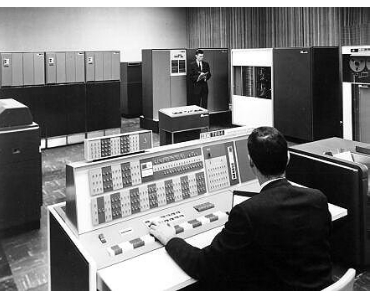
\includegraphics[width=.8\linewidth]{IBM7094.jpg}
  \end{sidecaption}
\end{figure}

En parallèle du perfectionnement des machines et de leur puissance de calcul apparaissent des langages de programmation qui vont faciliter la construction et la diffusion des méthodes de simulation. Nous n'envisageons pas d'en faire un historique complet, mais nous en donnons un aperçu dans l'encadré \enquote{Les premiers langages de programmation}.

\begin{framewithtitle}[Les premiers langages de programmation]{ Les premiers langages de programmation }

La période 1955 - 1965 est une période où la simulation est reconnue comme une méthode de résolution d'un certain nombre de problèmes difficilement tractables mathématiquement.\autocite{Nance1993, Ackoff1961} Des programmes de développement visant à mettre en place des modèles de représentation, de description nécessaire et facilitant la construction de simulations se multiplient. Deux classes de langage informatiques vont voir le jour durant cette période, et vont continuer à se développer et à s'influencer chacune de leur coté jusqu'à encore aujourd'hui. D'une part, les langages de plus haut niveau qui apparaissent ont pour vocation de se positionner comme une alternative plus expressive que l'assembleur. Dans cette optique le premier compilateur FORTRAN apparaît en 1957,  Algol en 1958, Cobol en 1959, et Lisp 1958. Ces langages et leur successeurs sont d'usage assez générique, et permettent de décrire correctement tout types de programmes. Toutefois à l'époque de leur apparition ils sont d'accès relativement difficiles pour une personne non initiée, ce qui nous amène au développements sur la même période d'une deuxième catégorie de langage, plus spécialisée dans la construction spécifique de modèle de simulation. \autocite[239]{Naylor1966}

A la même époque, des langages spécialisés dans l'expression des simulations apparaissent, et pour la plupart s'appuient et évoluent en parallèle des développements des langages classiques sur lesquels ils s'appuient. Ces SPL ( \foreignquote{english}{Simulation Programming Langages}) comme Simula en 1962, ou bien Dynamo en 1958 ont ceci d'intéressant qu'ils ont très largement accompagné les formidables avancées conceptuelles de cette époque et cela au travers des différentes disciplines. Ainsi la première période 1955-1960 est marquée par la mise au point de GSP (\foreignquote{english}{General Simulation Program}) par Owen et Tocher \autocite{Tocher1960}. Celui-ci est considéré comme le tout premier langage mis au point pour faciliter la description de simulation sur ordinateur. Un effort que Tocher va accompagner d'une publication phare en 1963 dans le livre \foreignquote{english}{Art of Simulation} \autocite{Tocher1963} . Vient ensuite une autre génération de langage en 1960-1965 comme GPSS (\foreignquote{english}{General Purpose System Simulator}), Simscript (développé sous l'impulsion de la RAND corporation), et la première version du langage SIMULA, qui donnera naissance à la fin des années 1960 à Simula-67, un langage qui aura un impact dépassant largement la classe des SPL, et inspirera les créateurs des futurs langages objets comme Alan Kay, auteur plus connu comme le créateur du premier langage objet SmallTalk. 

%% FIXME ORTHOGRAPHE DEUX PARAGRAPHE CI DESSOUS
On trouve plus d'information sur cette période spécifique abordé sous l'angle de l'ingénierie logicielle dans les publications de \textcites{Nance2013,Nance1993, Araten1992, Nance2002} et en consultant les \href{http://informs-sim.org/}{@archives} de la WSC (Winter Simulation Conference). Cette dernière, si elle n'est pas la première à aborder cette thématique (le \textit{System Simulation Symposium} en 1957 selon Nance), est la première à vouloir péréniser le débat à un niveau national \autocite{Nance2002}. Fondé en 1967 \autocite{Crain1992, Araten1992} celle-ci jouit aujourd'hui d'une très large visibilité au niveau international, notamment car elle abrite les publications de pionniers et de membres importants pour la discipline simulation. On pourra citer par exemple Sargent et Balci, des pionniers dans la construction de la discipline de la Validation \& Verification, qui participe et publie régulièrement pour cette conférence. 

Dernièrement les \textit{procedings} héberge le récit sur plusieurs années d'un projet \autocite{Nance2013} réunissant les acteurs important dans l'histoire de la simulation autour d'une fondation oeuvrant pour la récolte de témoignages vidéo, audio et la préservation, mise à disposition de tous des documents initiaux fondateurs, le \href{http://d.lib.ncsu.edu/computer-simulation/}{@Computer-Simulation-Archive} hébergé par la \textit{North Carolina State University}

\end{framewithtitle}

\Anotecontent{marble_computer_historycdc}{ \textcite[3]{Marble1967} déclare dans son recueil de programme de 1967 avoir écrit des routines pour le CDC 3400, que l'on suppose rapidement traduit en CDC 6400. Une procédure qui semble courante, comme en témoigne \textcite{Goldberg1968} pour le package \textit{SPURT} dédié à la simulation créé et utilisé (apparemment même par des géographes) au \textit{Vogelback Computing Center} alors sous la direction de Mittman. En 2010 Marble écrit \foreignquote{english}{Northwestern, when I arrived, was just opening its new Vogelback Computing Center and had acquired high end computing technology in the form of a Control Data Corporation (CDC) 6400. Aside from the “super”computer, the most significant component of Northwestern's computing infrastructure, in my eyes, was clearly Vogelback's Director of Computing, Dr. Benjamin Mittman. Ben was the originator of computer chess as a competitive programming activity, and he put together a generally excellent support staff at Vogelback. He was immensely helpful on a personal level to those of us who were working on the CDC mainframe. Ben also made sure that a number of useful software packages (e.g., the BMD statistical analysis package, linear programming software for solution of the transportation problem, etc.) were made freely available to all Vogelback users.} \autocite{Marble2010} Anecdote amusante sur le personnage cité par Marble, Benjamin Mittman est aussi un acteur important dans le développement et la structuration de la communauté créant des programmes d'échecs sur ordinateur, et accueille au \textit{Vogelback Computing Center} les étudiants David J. Slate, Larry R. Atkin, et Keith Gorlen ayant donné naissance au programme pionnier \textit{CHESS} \autocite{Mittman1971} s'executant sur le tout récent \href{http://computerchess.tumblr.com/post/56345790213/playing-chess-at-vogelback-computing-center}{@CDC6400}, vainqueur plusieurs années d'affilé dans les premières compétitions d'échec organisés à l'époque par l'ACM \href{https://chessprogramming.wikispaces.com/ACM+North+American+Computer+Chess+Championship}{@ACM}}

\Anotecontent{ibm604650}{Voir \href{http://www.aag.org/cs/garrison}{@Garrison} et la page \href{https://www.washington.edu/uwit/history/}{@historique} du service IT (information technology) de l'université de Washington}

D'un point de vue technique \textcite{Haggett1969} cite comme véritable point de départ dans la discipline la  démocratisation de l'accès à la ressource informatique après 1961, avec la diffusion d'une deuxième génération d'ordinateurs dans les grands centres de calculs, en partant notamment de la série IBM 7094, le \textit{Vogelback Computing Center} ouvert en 1965 à Northwestern avec un CDC 3400 apparemment très vite completé avec la sortie du CDC 6400 sur lequels vont travailler des pionniers comme Marble \Anote{marble_computer_historycdc}. Des ordinateurs que l'on imagine beaucoup plus accessibles et performants que la précédente série IBM 604 et 650 à \textit{vacuum tube} utilisé au début des années 1960 à l'université de Washington\Anote{ibm604650}, des précurseurs qui seront rapidement remplacés, par exemple par l'IBM 1620 enfin utilisable avec le langage Fortran I \autocite[66]{Berry2005}. 

\Anotecontent{ordinateur_actuel}{En comparaison, les ordinateurs actuels contiennent au minimum 4Go de mémoire, soit 4 194 300 KB.}

En Nouvelle-Zélande, Golledge nous indique que l'installation sur le territoire de la firme IBM semble précéder de peu la formation des pionniers \autocite[94]{Bailly2000}, et au début des années 1960 l'université de Canterbury se porte acquéreur d'un flambant neuf IBM 1620 doté de 32K de mémoire.\Anote{ordinateur_actuel}

\Anotecontent{histoire_suede}{Une récolte de documents publique nationale a été organisé par le \textit{tekniskamuseet} de Suède, les textes sont disponibles à l'adresse internet suivante \href{http://www.tekniskamuseet.se/it-minnen}{@tekniskamuseet}}

En Suède \Anote{histoire_suede}, trois ordinateurs sont construits dans le courant des années 1950-60 : SARA par la société Saab à Linköping, DASK à l'institut scientifique de Copenhague, et SMIL à l'université de Lund \autocite{Persson2007}. Carl Erik Frödberg, un ami d'enfance de Hägerstrand, fait partie avec Eric Stemme des consultants amenés à échanger sur le sol américain avec les leaders du domaine (Neumman, etc.) afin de démarrer le programme suédois.  SMIL est capable de compiler de l'Algol, et c'est probablement sur celui-là que Hägerstrand assisté de Frödberg a pu exécuter ses premiers programmes. En 1969, un Univac 1108 est acheté pour faire suite à SMIL \autocite[33-34]{Lindgren2008}.

En France, en 1955 il y a exactement six ordinateurs \autocite[3]{Armatte2008}, mais c'est seulement en 1970 que l'université Paris 1, centre de référence pour les géographes pionniers quantitativistes, se dote d'un ordinateur Philips et d'un terminal en contact avec le calculateur d'Orsay.

Toutefois, on ne peut parler d'une véritable démocratisation de l'outil informatique chez les chercheurs qu'avec l'apparition dans les années 1970 aux États-Unis des premiers postes informatiques individuels, et il faudra encore attendre le milieu des années 1980 pour que cette technologie se diffuse véritablement et touche le grand public.

A cette période la mise en oeuvre de modèles de simulation est fortement limitée par des problématiques humaines et techniques \autocites{Haggett1969}[387]{Marble1972}, dont on peut constater dans les ouvrages inter-disciplinaires vus dans la section précédente, qu'elle ne touche pas en réalité que la géographie \autocite{Guetzkow1972}.

C'est toutefois dans cette période où les compétences informatiques nécessaires à la programmation se font encore très rares, les langages de programmation multiples et peu stables, le matériel coûteux et peu disponible (nécessitant des opérateurs de saisie, temps d'utilisation partagé entre différentes disciplines, accessible seulement localement), que des packages de programmes sont peu à peu publiés et mis à disposition des chercheurs via les réseaux universitaires \autocite{Haggett1969}. 

Au niveau de ces réseaux de diffusion de programmes, selon \textcite[20-21]{Greer1972} deux sont à noter : \textit{the State Geological Survey of University of Kansas (Computer Contributions)}  et \textit{ the Department of Geography of the University of Nottingham U.K. (Computer Applications in the Natural and Social Sciences) }. Au niveau des progiciels, \textcite[20-21]{Greer1972} identifie en 1972 trois pôles universitaires importants : Iowa \autocite{Wittick1968}, Northwestern \autocite{Marble1967}, Michigan \autocite{Tobler1970c}\footnote{Ces progammes sont malheureusement impossibles à trouver, et les publications ne sont disponibles que sous la forme d'archives numérisées non exploitables (\textit{Google Books}), ou sous format papier dans les universités correspondantes. Un travail reste à faire pour sauvegarder et mettre ce bien commun à disposition de tous les géographes.}. En effet, des pionniers comme Marble ou Tobler mettent à disposition dans le courant des années 1960 différentes routines informatiques en libre accès, \textcite[3]{Marble1967} parle de 150 routines développées jusqu'à 1967, et cela seulement à Northwestern dans le département de géographie. Le premier \textit{Statistical package for Social Science} pour les sciences sociales (ou \href{http://www.spss.com.hk/corpinfo/history.htm}{@SPSS}) date quant à lui de 1968 \autocite{Barnes2011}, alors que sort à la même date l'ouvrage \foreignquote{english}{best-of} de \textcite{Berry1968} \foreignquote{english}{Spatial Analysis: a Reader in Statistical Geography}, qui offre une vision d'ensemble des derniers développements statistiques et mathématiques.

\Anotecontent{programmes}{Particulièrement difficiles à trouver en dehors des Etats-Unis, voici un exemple des rapports disponibles dans les \href{http://findingaids.library.northwestern.edu/catalog/inu-ead-nua-archon-989}{@archives} de la \textit{Northwestern University Library} contenants les précieux programmes et les rapports d'avancements de ces ingénieurs géographes : a) \textit{Duane F. Marble and Sophia R. Bowlby, Computer Programs for the Operational Analysis of Hagerstrand Type Spatial Diffusion Models, Research Report No. 27, February, 1968} ; b) \textit{Duane F. Marble, Some Computer Programs for Geographic Research, Special Publication No. 1, August, 1967 } c) \textit{ Forrest R. Pitts, Hager III and Hager IV: Two Monte Carlo Computer Programs for the Study of Spatial Diffusion Problems, Research Report No. 2, October, 1965}}

En faisant régulièrement état de leur avancements dans divers rapports ou publications\Anote{programmes}, les pionniers Marble, Morrill, Pits et Bowlby \autocite{Pitts1963} qui se placent dans la continuité des premiers travaux relatifs aux processus de diffusion d'Hägerstrand \autocite{Hagerstrand1953, Hagerstrand1967a} donnent ainsi à voir les efforts et les difficultés auxquelles la petite équipe doit faire face pour améliorer les programmes, ou les adapter à des problématiques différentes.

Sur un tout autre front, celui du développement des \textit{large scale models} \autocites[8]{Batty1976}, les universitaires géographes sont plus souvent cités comme spectateurs qu'acteurs \autocite[9]{Batty1994}, cela même si quelques universitaires arrivent à décrocher des contrats importants \autocite{Barnes2006a} pour des études plus pratiques, comme \textcite{Garrison1959}, nottamment du fait que les objectifs poursuivis sont relativement différents, la planification et la prédiction prenant plus souvent le pas sur la curiosité et l'explication scientifique. Toutefois, et si on en croit \textcite{Haggett1969} la communauté universitaire semble attendre beaucoup des retombées de ces grands programmes, qui disposent de moyens humains et économiques importants pour développer des programmes et collecter des données.

Si le requiem de \textcite{Lee1973} a bien eu un effet non négligeable sur la construction et la publication de tels modèles du coté des planificateurs \footnote{Seulement trois modèles seront publiés dans le même journal à la suite de cet article ...}, force est de constater que la construction de modèles de simulation pour la théorie urbaine ne disparaît pas dans cette période \autocite[11-12]{Batty1994}, et s'appuie au contraire sur l'apprentissage de ses échecs pour se réinventer dans les années qui suivent. A ce titre, \textcite{Harris1994} soulève dans une relecture très critique de l'article de Lee, l'ignorance ou la méconnaissance de l'auteur vis-à-vis des débats qui agitent déjà depuis plusieurs années la simulation de modèles urbains \autocites{Batty1971, Wilson1970, Orcutt1957, Harris1968}. Ce faisant, Harris accuse Lee d'enfoncer des portes ouvertes et de porter des accusations que certains jugeront par la suite prématurées vis-à-vis du préjudice subi, touchant à cœur une discipline d'à peine une décennie et encore en phase d'apprentissage. \autocite[p11]{Batty1994}.

Ce mouvement de modélisation doit faire face à l'expression de ces limitations pour se reconstruire, limitations dont on sait par avance qu'elles ne seront pas seulement levées par la seule amélioration des techniques. Ainsi pour \textcite[11]{Batty1976}, de façon plus importante que tous les autres problèmes, c'est la révélation dans l'observation de cette richesse et de cette complexité d'interactions des facteurs causaux à l’œuvre dans l'évolution et la structuration des phénomènes urbains qui va le plus contribuer à la réévaluation des formes de modélisation. \footnote{Une analyse qu'il reprend dans son article de 2001 \autocite{Batty2001}, axée essentiellement autour de l'évolution de l'articulation des mécanismes internes aux modèles et aux répercussions que cela entraîne dans la construction et la validation des modèles.}

D'une part l'emploi de théories trop simplistes, induit indirectement la nécessité d'un retour à une démarche inductive plus exploratoire \footnote{On notera par exemple le témoignage de \textcite{Boyce1988} lorsqu'il dit à propos des chercheurs engagés dans cette voie \foreignquote{english}{Some, including myself, turned to more empirically oriented research activities, perhaps in the hope of strengthening the foundation of future models}}, jusque là mise de coté. 

D'autre part, une autre voie d'évolution possible pour les modèles vient des travaux existants réalisés dans d'autres disciplines universitaires ou dans le monde industriel. Ainsi différentes équipes de développements sont déjà bien identifiées dans la communauté des économistes comme \textcite{Orcutt1960} et son premier modèle micro \foreignquote{english}{bottom-up} développé à l'\textit{Urban Institute}, les démographes sur les modèles de migrations inspirés des travaux d'Orcutt comme REPSIM, puis POPSIM; sans oublier l'apport de \textcite{Forrester1961} sur l'optimisation industrielle, une des branches opérationnelles d'inspiration la plus directe du projet systémique au début des années 1960 \autocites{Cohen1961}[911]{Shubik1960b}.

% et Hagerstrand ? 
La \enquote{micro-simulation} initiée par Orcutt, qui semble effectivement passer outre l'extinction annoncée par Lee en 1973, rencontre même un certain succès durant toutes les années 1970 comme en témoigne la mise en place de nombreux programmes nationaux au début des années 1980. \autocite{Baroni2007} Une réponse à cette survie peut être avancée dans le positionnement innovant d'Orcutt pour faire face aux résultats décevants des \textit{Large Scale Models} de son époque, opérant pour la plupart à un niveau macro et fournissant des résultats hautement agrégés difficiles à exploiter dans un cadre prédictif, et finalement peu représentatifs de la diversité des systèmes économiques \autocites{Birkin2012, Baroni2007}. Si les critiques de Lee peuvent pour la plupart être mobilisées pour critiquer les modèles issus de la micro-simulation (complexité des modèles, absence d'objectifs clairement posés, volume des données à mobiliser, complexité des calculs, coût de construction, absence de résultats, etc.), il n'en reste pas moins que la proposition d'Orcutt introduit avec une approche plus \textit{bottom-up} une dimension explicative absente jusque là. En répondant à l'observation de Lee sur l'absence d'extraction de connaissances micro quelque soit la complexité injectée dans les modèles macro, Orcutt ouvre d'une certaine façon la voie à des développements théoriques beaucoup plus riches que ne le permettaient à l'époque les seuls modèles macro, faisant ainsi de son modèle un instrument pour \foreignquote{english}{consolidating past, present, and future research efforts of many individuals in varied areas of economics and sociology into one effective and meaningful model; an instrument for combining survey and theoretical results obtained on the micro-level into an all-embracing system useful for prediction, control, experimentation, and analysis on the aggregate level} \autocite[122]{Cohen1961}.

D'un autre coté, cette micro-simulation telle que déjà théorisée par Hägerstrand dans sa version spatiale ou par Orcutt dans sa version économique, va étonnamment et cela pendant plusieurs années rester un courant ayant peu d'impact sur le développement des modèles urbains en économie spatiale \autocite[5]{Sanders2006}, et cela malgré plusieurs appels d'un coté \autocite{Hagerstrand1970} ou de l'autre \autocite[5]{Isard1998}. De façon indépendante et dans un univers somme toute limité par de fortes contraintes techniques et financières, ces travaux vont toutefois dans leurs lentes et multiples convergences donner naissance autant à des modèles universitaires qu'à des programmes nationaux (DYNASIM et CORSIM pour Orcutt aux Etats-Unis, SVERIGE en Suède, etc.). Pour finir cette parenthèse sur la micro-simulation par une petite transgression temporelle, si peu de modèles existent encore dans les années 1990, plusieurs publications récentes font état d'un inversion de la tendance ces vingt dernières années \autocite{Lenormand2013}, avec une augmentation (et une diversification ? ) croissante des modèles, sûrement liée à des capacités de développements informatiques plus importants, tant du point de vue des données, que de la puissance d’exécution qui admet l'importance croissante du parallélisme, idéale pour simuler des entités individuelles. \autocites[5]{Sanders2006}{Lenormand2013}

Cette crise, qui on l'a vu touche avant tout les instituts de planification américains couverts par la RAND, va fournir \textit{post mortem} le terreau nécessaire à la transformation d'une discipline dont le rayonnement dans la communauté scientifique à l'international ne va aller qu'en s'amplifiant après 1970 (voir la carte \ref{fig:S_carte_wegener}).

\begin{figure}[h]
\begin{sidecaption}[fortoc]{La carte des centres de recherches les plus actifs à la fin des années 1980, début des années 1990 selon \textcite{Wegener1994}}[fig:S_carte_wegener]
  \centering
 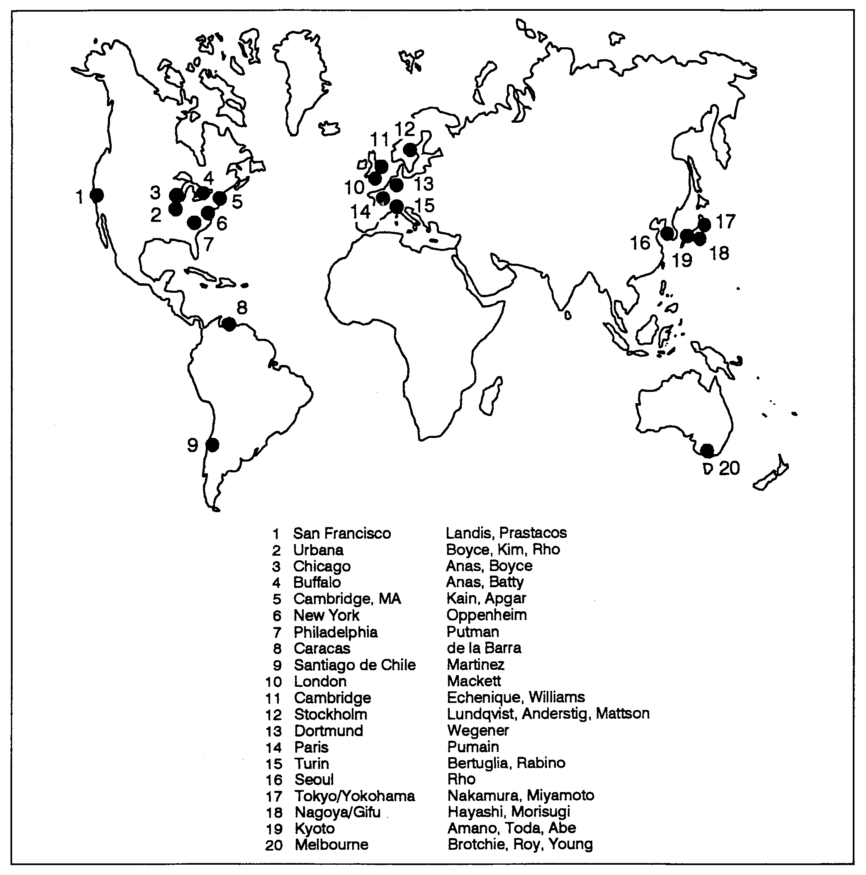
\includegraphics[width=.9\linewidth]{carte_wegener.png}
  \end{sidecaption}
\end{figure}

C'est le cas par exemple au Royaume-Uni où sont récupérés les modèles américains ayant donné de bons résultats, comme celui de Lowry \autocite{Lowry1964}, pour servir de base à de nouveaux travaux mettant en perspective l'influence ou les progrès d'autres courants disciplinaires en contact avec la géographie. 

Le mouvement du professeur Orcutt \autocite{Orcutt1957}, mais aussi celui de Forrester \autocite{Forrester1961, Forrester1969} font dans leur implémentation dynamique alors écho aux travaux initiaux du géographe Hägerstrand, et poussent dans cette période de reconstruction toute une partie des géographes à réintégrer la dimension temporelle à des modèles d'optimisation statique en échec. \autocite[p295]{Batty1976}.

La diffusion et la généralisation du programme systémique permettent aux géographes d'accéder à tous les outils conceptuels et surtout opérationnels \autocite{Forrester1969} nécessaires pour penser, modéliser et simuler les systèmes géographiques au travers de leurs interactions complexes, en intégrant dans leurs analyses cette hétérogénéité d'échelle caractéristique des objets géographiques, comme peut l'être par exemple la région.

Si les universitaires américains semblent rater le coche de cette transformation, en Europe plusieurs écoles viennent à se former, comme la \foreignquote{english}{social physics} de \autocite{Wilson1970} dont l'émergence est considérée comme un moment important dans le renouveau des modèles urbains \autocite{Griffith2010}; mais également d'autres écoles comme celle de Peter Allen, qui s'appuient sur l'évolution des mathématiques et le transfert méticuleux de concepts observés en physique pour construire des modèles à la fois spatiaux et dynamiques capables de simuler de façon plus réaliste les interactions complexes intervenant dans la formation et l'évolution des villes. \autocite[11]{Batty1976, Batty2001} \autocite[27-28]{Pumain2003} \footnote{ Pumain liste au moins trois intérêts qui découlent de cette phase d'acquisition du projet systémique : a) le dépassement de l'opposition idiographique et nomothétique, b) l'histoire et les particularités des entités géographiques vues comme expression originale de trajectoires et de bifurcations, c) le dépassement de la rigidité des trajectoires biographiques historiques par l'emploi des simulations}

\textit{Dans quelles mesures les problématiques levées à la fin de la section précédente ( section \ref{ssec:disciplines_touches}) sont-t-elles encore pertinentes après une telle évolution des pratiques dans la géographie ? }

L'amélioration de la formation des géographes européens, et notamment des géographes français dans les années 1970, permet à ceux-ci d'intégrer plus facilement les évolutions de l'informatique durant les années 1970-1990, leur garantissant ainsi une certaine autonomie de développement qui va donner lieu à plusieurs collaborations fructueuses avec les physiciens \autocite{Pumain1984}; 

Concernant l'accès à la ressource informatique pour construire et explorer les modèles de simulation, même si les conditions se sont améliorées avec la démocratisation de l'ordinateur, celle-ci reste un élément bloquant pour l'exécution et l'exploration des modèles de simulation.

Tout d'abord, il y a ce témoignage\footnote{Ce témoignage est issu d'un échange par mail en 2013} précieux de Duane Marble, un des pionniers modélisateurs américains, qui lorsqu'il est interrogé sur la suite des problématiques de validation des modèles de simulation détaillées dans son article de 1972 \autocite{Marble1972}, conforte d'une certain façon notre point de vue : \foreignquote{english}{As I recall, the situation in the 1980's had not changed very much. Simulation in human geography did not last long. Much of this was the result of a lack of computer capacity. Simply replicating Hagerstrand's diffusion model proved difficult and our attempt to inject a more explicit temporal element just would not work due to the computational load.}

Malgré les apports heuristiques indéniables qui vont avec l'utilisation de l'outil, on retrouve l'expression de difficultés concernant le calibrage des modèles plus complexes chez de nombreux auteurs pionniers modélisateurs \autocites{Batty1976, Pumain1998a}[400]{Sanders1984}, notamment pour ce qui concerne le calibrage des modèles, souvent difficile pour ces modèles dynamiques non linéaires soumis à de tels fluctuations dans leur comportements. Voici comment \autocite{Pumain1998a} résume les difficultés opérationnelles résultats de plusieurs années de travaux menés autour des modèles de simulation dynamiques non-linéaires opérant dans le cadre de la théorie de l'auto-organisation : \enquote{Les difficultés de calibrage, associées à la capacité élevée de bifurcation des modèles, ont été maintes fois décrites, de même que l’impossibilité de valider comme \enquote{meilleur ajustement} une configuration donnée de paramètres.}

Batty est probablement un des premiers géographes à faire ce travail d'état de l'art des techniques de calibrations disponibles et applicables à cette nouvelle classe de modèles urbains. Des méthodes de calibration basées sur des méta-heuristiques de type descente de gradient, sont déjà utilisées par les géographes comme \textcite[159]{Batty1976} pour résoudre des problèmes d'optimisations utilisant les sorties de modèles. Toutefois ces méthodes sont encore trop souvent limitées à des modèles à 1 ou 2 paramètres, et s'avèrent peu robustes face à des problèmes acceptant des minima locaux. 

Une chose est sûre pour ce qui est de la recherche de paramètres, on perçoit très tôt chez certains géographes la nécessité d'optimiser cette étape, rendue improductive et dangereuse du fait de la non-linéarité des modèles \enquote{The trial and error method of searching for best-parameter values by running the model exhaustively through a range of parameter values or combinations thereof represents a somewhat blunt approach to model calibration.}

L'appel à l'utilisation de nouvelles méthodes pour l'exploration des modèles déjà lancés par \textcite{Batty1976}, est par la suite repris de façon implicite par \textcite{Openshaw1996}. Celui-ci publie en 1996 avec un collègue de Leeds un article sur les algorithmes génétiques, la méthode la plus efficace disponible alors pour explorer des espaces de paramètres de façon efficace. La conclusion est explicite :

\foreignquote{english}{The results demonstrate that even GA en ES can provide very good solutions for spatial interaction model calibration, albeit sometimes at the expense of considerable extra compute times. [...] It would also be worth considering the use of other forms of global optimization method; [....] As computer hardware becomes faster, the attraction of simple, relatively assumption-free, and highly robust approaches to global parameter estimation can only grow and allow the geographical model builder to worry less about the problems of parameter estimation and focus more on the task of model design.}\autocite{Openshaw1996}

La course à la puissance informatique nécessaire pour explorer et calibrer les modèles ne fait en réalité que commencer. Les méthodes sont encore en cours de développement, et leur usage s'avère extrêmement coûteux sur le plan informatique.

Se pose alors la question suivante, l'incapacité à calibrer un modèle de simulation n'est-elle pas un problème qui limite de facto l'évolution en crédibilité de l'outil simulation ? 

Concernant ce problème plus large de la validation, dont le calibrage n'est qu'une facette, le changement de paradigme explicatif et l'ouverture sur la complexité a soulevé un débat qui dépasse en réalité la seule problématique technique. Il ne suffit plus de garantir un résultat pour que le modèle soit considéré comme valide, sa structure causale est elle aussi considérée comme le résultat d'un processus social, et dont la contenance doit normalement être validée terme à terme avec le domaine empirique; or c'est celle-là même qu'on ne peut observer dans le cadre d'un système complexe. (cf \textit{observational dilemna} de \textcite[296]{Batty1976} :

\foreignquote{english}{Perhaps the major problem concerns the ability to observe or monitor the urban system. Unlike the physical sciences in which the effect of critical variables on the system of interest can be isolated in the laboratory, such a search for cause and effect is practically impossible in social systems. Thus, there are many instances when it is difficult, if not impossible, to disentangle one cause from another in the changing behaviour of such systems. This is a fundamental limitation which is referred to here as the observational dilemma.}

La dernière phrase d'Openshaw prend alors tout son sens, et en nous rappelant que la construction de modèle est un processus incrémental, il fait indirectement écho à l'évaluation elle aussi incrémentale d'une structure causale où chaque mécanisme lorsqu'il est ajouté/enlevé, remet en cause l'exploration précédente. Dès lors, la systématisation de cette calibration devient \textbf{le seul moyen de garantir une construction} qui serait faite en tout connaissance de cause, en mesurant, et donc en discutant l'apport de chacune des hypothèses durant le processus de calibration.

La dépendance à la ressource informatique se renforce en réalité encore un peu plus avec la nécessité d'explorer les modèles, non plus lorsqu'ils sont terminés, mais dès que la première brique est posée. 

%%FIXME : A MODIFIER POUR COLLER AVEC LE PARAGRAPHE PRÉCÉDENT %%
%Paradoxalement il donne aussi à voir les limites des approches proposées pour létude de l'homme dans son environnement, et offre ainsi le matériel idéal pour appuyer la formulation critique des géographes radicaux marxistes, un mouvement qui s'amplifie dès le début des années 1970 en parallèle avec la conjoncture politique nationale et mondiale. \autocite{Golledge2006}


%Ainsi les progrès fulgurants de l'informatique, l'apparition de nouveaux langages exclusivement orientés pour la simulation comme Dynamo, la prise de conscience tout au long des années 1960-70 des défauts de cette première génération de modèles, et les changements d'objectifs de la discipline \autocite[12]{Batty1994} \autocite{Boyce1988} autorisent (voire recommandent) la formation de nouveaux modèles. Ceux-ci sont conçus comme plus parcimonieux, autorisant les démonstrations plus abstraites \autocite{Forrester1969}, plus orientées vers la compréhension des mécanismes à l’œuvre que sur la prédiction (un retour sur les modèles théoriques est opéré), intégrant plus facilement l'hétérogénéité dans la nature des dynamiques (rétro-action, non linéarité) des processus \autocite{Forrester1969, Wilson1970, Allen1978}, et ouvert à l'intégration d'autres dimensions explicatives à l'oeuvre dans la formation des processus, comme ceux déjà explorés l'individu et le temps \autocite{Hagerstrand1967a,Orcutt1957,Forrester1961}. En lisant les articles de Pred, d'Olsson \autocite{Olsson1969,Olsson1970}, de Curry, on percoit chez les nouveaux économistes spatiaux cette volonté de changement, avec la reintroduction de la stochasticité et des modèles probabilistes, l'intégration du temps dans les modèles, mais aussi les causalités multiples.

% PLUSIEURS points développement méthodologiques accompagnant renouvellement théoriques accompagnant nouvelle géographie : Hagerstrand , Orcutt -> causalité + individualisme méthodologique,  Forrester -> complexité
% Hagerstrand premiere utilisation montecarlo en science sociale, vient a Washington et rencontre Morril... qui pour Benko Stromayer marque troisieme theme dominant le bouleversement quantitatif) Gould2004

% simulation permet de développer cette causalité ...
% Systeme dynamique, non linéarité, permet avancée fondamentale dans les questionnements, révélateur aussi de l'apport des techniques / méthodologies...
% Basculement vers explicatif !


% -*- root: These.tex -*-

\section{La validation des modèles de simulation}
\label{sec:constante_problematique}

\hl{CORRECT}

Les termes \foreignquote{english}{Validation \& Verification} tels que définis par les institutions de normalisation sont conçus comme génériques et valables pour des disciplines autres que l'ingénierie logicielle (section \ref{ssec:triple_lecture}). Dans ce sous-ensemble de pratiques, la simulation dispose de sa propre branche historique, dans laquelle des spécialistes raffinent et organisent depuis les années 1960 ces notions en mettant en oeuvre des typologies d'outils et des méthodologies de conception et d'évaluation standardisées \autocite{Nance2002}. Ces définitions sont parfois reprises pour encadrer des travaux en sciences humaines et sociales, qui cotoient aussi une utilisation de ces termes en philosophie des sciences. L'ambiguité et le mélange des termes dans les publications semblent aussi courant que les débats sans fin \autocite{Numo2007,Augusiak2014}, ce qui nous obligent à regarder de plus près comment ces termes sont employés dans différentes disciplines (section \ref{ssec:triple_lecture}). Trois branches utilisant ces termes seront abordées : le courant historique de la V\&V (section \ref{sssec:def_generique_validation}), la philosophie des sciences (section \ref{sssec:philo_sciences}) , et la communauté des proches modélisateurs (section \ref{sssec:validation_modelisateurs}).

% ssec:transition_annee70
% sssec:realite_neopositiviste
% sssec:progressive_systemique
% sssec:forrester_impact

La généricité et le manque d'incarnation géographique du point de vue de la \textit{V\&V}, l'approche philosophique très éloignée des pratiques ou la tendance à remarquer cette problématique de la Validation comme liée à une technologie particulière, sont des arguments qui nous poussent à reposer cette question de l'explication par la modélisation en prenant en compte son inscription historique.

Comme déjà entrevu à la fin du chapitre 1 (section \ref{ssec:crise_mutation}), les années 1970 sont considérées comme des années charnières. Il sera intéressant de mettre en perspective les arguments d'une géographie radicale critique des approches modélisatrices (néo-positivisme, fétichisme spatial \Anote{fetichisme_spatial}, etc.) avec la réalité des transformations touchant une branche quantitative en pleine évolution.

La section \ref{sssec:realite_neopositiviste} propose de déconstruire avec les arguments disponibles ce point de vue qui voit dans l'application pratique de la méthodologie néo-positiviste un support crédible à l'explication dans la construction de modèles en géographie (section \ref{sssec:realite_neopositiviste}). Une fois cette proposition écartée, on peut s'intéresser à la diffusion des prémisses systémiques \autocites{Chorley1962, Berry1964a, Haggett1965,Harvey1969} semés par les géographes des années 1960 \ref{sssec:progressive_systemique} et soulever ainsi cette montée en puissance pertinente d'un paradigme explicatif très différent \autocite{Besse2000} des cadres logiques jusqu'alors empruntés aux influents Viennois Hempel ou Popper.


% ssec:evaluation_construction
% sssec:hermann_contexte
% ssec:confrontation_sysmodelise_sysobserve
% sssec:equifinalite

Pour \textcites{Batty2001, Batty2005b} c'est le modèle \textit{Urban Dynamics} de \textcite{Forrester1969} qui cristallise le mieux ce changement de point de vue chez les modélisateurs de l'urbain (section \ref{sssec:forrester_impact}). Une transformation dans la façon de penser la construction des modèles qui s'accompagne aussi d'un certain regain d'intérêt \autocite{Batty1976} pour des branches de développement ayant toujours abordé la modélisation sous un angle \textit{bottom-up} et spatio-temporel en géographie \autocites{Hagerstrand1952, Hagerstrand1967, Morrill1965, Morrill1965b, Marble1972, Ward1973} \Anote{marble_decline} ou dans des disciplines connexes \autocite{Orcutt1957}.

Il est alors intéressant de confronter le point de vue assez neuf de Forrester vis-à-vis de la construction des modèles et de la Validation, avec ceux des géographes et des courants de pensée de l'époque sur cette question, dont on a vu au chapitre 1 qu'elle arrive dans les débats sur la simulation dès la fin des années 1960 \autocites{Naylor1967, Hermann1967, Dutton1971, Guetzkow1962, Guetzkow1972}

De Naylor à Hermann, on observera dès les années 1970 une grande différence dans la façon de traiter la validation des modèles (section \ref{ssec:evaluation_construction}). C'est en partant ensuite des propositions très actuelles (section \ref{sssec:hermann_contexte}) posées par \textcite{Hermann1967} que l'on introduira les débats les plus récents sur cette question de la validation. L'objectif étant de déconstruire cette notion (section \ref{sssec:confrontation_sysmodelise_sysobserve}) jusqu'à développer un cadre explicatif plus compatible avec la construction et l'évaluation des modèles de simulation dans notre discipline (section \ref{sssec:equifinalite}), la géographie.

%Il n'est pas  ici de relater en détail cette construction d'une géographie radicale, humaniste ou comportementale, on retiendra seulement que ces courants se forment principalement à la convergence de problématiques politiques (crises économique nationales et internationales, guerres), de revendications théoriques (rejet des méthodes quantitatives et accusation de \Anote{fetichisme_spatial}) et/ou méthodologiques (retour de l’herméneutique).


%Les acteurs prônant une démarche scientifique teinté de néo-positivisme largement inspiré des sciences physiques sont alors la cible idéale de ces nouveaux acteurs, et vont subir un large front de critique.

%Gregory, dont on mobilise le point de vue pour critiquer la vision néo-positiviste / positiviste en géographie, utilise ce dernier argument de façon conjointe avec la pensée d'Habermas pour charger les dérives entraînées par les méthodes quantitatives, et proposer un autre style de pensée axé sur la réconciliation d'un point de vue structuraliste, phénoménologique et critique pour entre autre éviter l'écueil du \enquote{fétichisme spatial} \Anote{fétichisme spatial}. A la lecture d'ouvrage comme ceux de Gregory, dont la démarche de dépassement n'est pas sans levée des critiques pertinentes, il nous semble a posteriori que sa vision du mouvement quantitatif est en partie biaisé, d'une part parce que la réalité des pratiques peut tout à fait s'éloigner des discours tenus par quelques leaders d'opinion, tel qu'Harvey ou Bunge, et d'autres part parce que les critiques externes au mouvement, comme Gregory font mine d'ignorer une partie des transformations qui opère depuis le début des années 1970 en interne dans les pratiques visés.

%Ainsi, afin de montrer que la discipline géographique n'a pas attendu l'émergence de tels discours parfois extrémistes, nous avons aperçu dans la section \ref{ssec:crise_mutation} que les modèles de simulation économiques spatialisés, ont adopté au vu de leurs maigres résultats une démarche plus explicative permise entre autre par l'évolution des moyens de simulations, et que cette confrontation avec la problématique de validation a été formulée comme centrale par les modélisateurs pionniers et cela de façon explicite dans des ouvrages collectifs abordant cette question \autocite{Marble1972}. Si sur le fond il n'y a rien de critiquable à vouloir développer un autre style de pensée en opposition de certains excès constatés relatifs aux usages de ces nouvelles méthodes quantitatives, sur la forme il en résulte chez certains géographes l'émergence d'un amalgame malheureux qui associe un peu trop rapidement méthode quantitative positiviste, et modèle d'inspiration économique néo-libéraliste . Cette dualité opposant géographe (et géographie) qualitativiste/quantitativiste n'est plus considéré comme constructive \autocite{Sheppard2001}.

%Outre le fait que cette ouverture s'accompagne d'innovations méthodologiques permettant l'opérationalisation des concepts, s'ouvrent en parallèle avec la chute du néo-positivisme de nouveaux débats autour de l'explication \autocite{Hedstrom2010} à la fois chez les praticiens (les \enquote{mécanismes générateurs} de Boudon, les \foreignquote{english}{causal-mechanisms} plus récents des biologistes, les \foreignquote{english}{generative mechanisms} d'Epstein) mais également chez les philosophes des sciences en biologie (Salmon, Machamer, etc.) où les thèses de Popper-Hempel, bien que souvent citées, sont en réalité rarement appliquées ou même appliquables dans les faits \autocite{Bechet2013}.

%Un retour sur la démarche de construction des modèles en géographie s'avère nécessaire pour comprendre les éléments qui nous ont échappé dans la continuité de cette problématique qu'est la validation des modèles. En s'appuyant sur les témoignage de \autocite{Batty2001, Pumain2003} on parvient très bien à décrire ce basculement opéré à la charnière des années 1970, alors même que les géographes accèdent peu à peu aux concepts opérant dans le paradigme systémique \autocite{Harvey1969}, et que l'insuffisance des démarches de construction de modèles devient prégnante.

%L'enjeu ici est d'autant plus important qu'il se double d'une réalité opérationelle, faisant des problématiques de sous-détermination (Quine) ou d'équifinalité (Bertalanffy) des concepts tout à fait tangibles, dont la manipulation déborde du cercle des philosophes des sciences pour venir parasiter les débats des modélisateurs en SHS, dont la qualité des explications avancées doit s'adapter à cet horizon, et se réinventer dans des discours, des méthodologies plus spécifiques.



% -*- root: These.tex -*-

\subsection{Une lecture pluridisciplinaire des problématiques liées à la validation}
\label{ssec:triple_lecture}

\subsubsection{Les définitions de la validation en V\&V}
\label{sssec:def_generique_validation}

Les termes \foreignquote{english}{Validation \& Verification} ou \textit{V\&V} proviennent à l'origine de l'ingénierie des systèmes et peuvent être rattachés au concept de \enquote{qualité} tel qu'il est défini par la famille de règles ISO établies par l'organisation mondiale de normalisation.

Décomposable en plusieurs branches cette discipline à part possède une branche dédiée à l'expertise logicielle. De ce fait, il n'existe pas réellement de définition ni de théories ou méthodologies officiellement acceptables, l'acceptation des termes pouvant varier fortement selon les branches d'application.

On trouve toutefois quelques références dans des livres dédiés à la terminologie standard pour la \enquote{gestion de projet} dans un large panel de disciplines, telle que le PMBOK (\textit{A guide to the Project Management Body of Knowledge}) \autocite{PMBOK2013}. Résultats d'un travail certifié par des associations ou des organismes étatiques tels que \textit{Institute of Electrical and Electronic Engineers} (IEEE) et \textit{American National Standards Institute} (ANSI), ce dernier propose une définition générale de ces termes pour l'ingénierie logicielle :

\foreignblockquote{english}[\cite{PMBOK2013}]{Verification and validation (V\&V) processes are used to determine whether the development products of a given activity conform to the requirements of that activity and whether the product satisfies its intended use and user needs.}

Celui-ci revient ensuite plus spécifiquement sur les termes, qu'il définit ainsi :

\begin{itemize}
\item \textbf{Validation} \foreignquote{english}{The assurance that a product, service, or system meets the needs of the customer and other identified stakeholders. It often involves acceptance and suitability with external customers. Contrast with verification.}
\item \textbf{Verification} \foreignquote{english}{The evaluation of whether or not a product, service, or system complies with a regulation, requirement, specification, or imposed condition. It is often an internal process. Contrast with validation.}
\end{itemize}

Les termes tels qu'ils sont définis sont finalement bien trop généraux pour envisager de les appliquer tels quels dans notre domaine de compétence. Dérivés de la branche de l'\textit{Operational Research (OR)}, les auteurs de la communauté restreinte des \textit{systems analysis or modelling and Simulation (M\&S) } engagent dès les années 1960-70 des efforts pour standardiser ces définitions pour la simulation.

Parmi les différents auteurs participant de ce mouvement ( Naylor, Finger, Oren, Hermann, Zeigler, Nance, Banks, Gass, Balci, Sargent, etc.), \textcite{Naylor1966} sont considérés avec West Churchman (1963) comme les tout premiers à avoir attiré et cristallisé \Anote{first_time_validation} dans de multiples publications l'attention sur cette problématique importante de la V\&V.

Formé à l'informatique dans la branche des \foreignquote{english}{management sciences} \autocite{Stricklin1985}, Naylor est un des premiers en 1967 \autocite{Naylor1967} à publier dans un article nommé \foreignquote{english}{Verification of Computer simulation models} une méthode abordant spécifiquement la question de la crédibilité des connaissances qui peuvent être apportées par un modèle de simulation. Une méthode qu'il va mettre spontanément en tension avec les débats qui agitent la communauté des philosophes à cette même période.

Malgré ses efforts et sa volonté de porter le débat loin dans la communauté interdisciplinaire (voir les premiers ouvrages collectifs sur l'usage de la simulation dans les \textit{behavior science} \autocites{Dutton1971, Guetzkow1972} ), la démarcation entre les deux termes reste encore peu claire à cette période \Anote{naylor_nance} \autocites[165]{Nance2002}[3]{Balci1986}.

Il faudra attendre le début des années 1980 pour qu'un standard émerge, grâce à des financements étatiques \autocite{Balci1986}, mais également du fait des efforts fournis par des auteurs comme Sargent et Balci \autocite{Nance2002}, qui collectent et organisent dans une typologie cohérente l'existant statistique et méthodologique, une activité qu'ils poursuivent encore aujourd'hui \autocite{Balci1998} \Anote{balci_standard}.

Pour \textcite[22]{Oberkampf2010} \foreignquote{english}{A Key milestone in the early work by the OR community was the publication of the first definitions of V\&V by the Society of Computer Simulation (SCS) in 1979 \autocite{Schlesinger1979}}. La SCS est un des instituts avec la U.S GAO (U.S General Accounting Office) à fournir des spécifications en 1979 \autocite{Balci1986}.

\begin{itemize}
\item \textbf{Model Verification} \foreignquote{english}{substantiation that a computerized model represents a conceptual model within specified limit of accuracy.}
\item \textbf{Model Validation} \foreignquote{english}{substantiation that a computerized model within its domain of applicability possesses a satisfactory range of accuracy consistent with the intended application of the model.}
\end{itemize}

Même si elles sont plus anciennes et de portée moins générale, ces définitions de la \textit{V\&V} semblent plus pertinentes, car évoquées plus régulièrement par les chercheurs en sciences sociales; les travaux les plus cités étant ceux de \textcite{Kleijnen1995}, ou \textcite{Sargent2010} qui placent leurs travaux dans la continuité de ces définitions. L'avancée de leurs travaux peut être suivie en feuilletant les \textit{Proceedings of the Winter Simulation Conference} où la problématique de la \textit{V\&V} est réévaluée régulièrement au regard des nouvelles connaissances. Ce schéma \ref{fig:S_VV} est devenu un classique repris et régulièrement amendé \autocite{Sargent2010}. Voici la lecture qu'en fournit \autocite{Oberkampf2010} :

\begin{figure}[htbp]
	\begin{sidecaption}[fortoc]{Un des tout premiers schémas issus de la publication de la SCS \autocites{Oberkampf2010,Schlesinger1979}}[fig:S_VV]
	  \centering
	 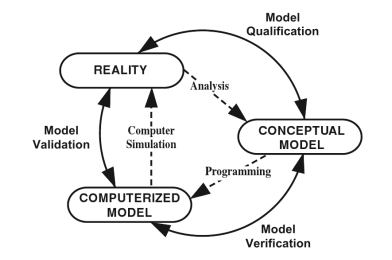
\includegraphics[width=.7\linewidth]{schelinger_schema1979.png}
	  \end{sidecaption}
\end{figure}

\foreignblockquote{english}[\cite{Oberkampf2010}]{The \textbf{conceptual model} comprises all relevant information, modelling assumptions, and mathematical equations that describe the physical process or process of interest. [...] The SCS defined \textbf{qualification} as \enquote{Determination of adequacy of the conceptual model to provide an acceptable level of agreement for the domain of intended application}. The \textbf{computerized model} is an operational computer program that implements a conceptual model using computer programming. Modern terminology typically refers to the computerized model as the computer model or code.}

Ce schéma a la particularité suivante, il \foreignquote{english}{ [...] emphasizes that \textbf{verification} deals with the relationship between the conceptual model and computerized model and that \textbf{validation} deals with the relationship between the computerized model and reality. These relationships are not always recognized in other definitions of V\&V [...]}

Autrement dit, \foreignquote{english}{The OR community clearly recognized, as it still does today, that V\&V are tools for assessing the accuracy of the conceptual and computerized models.} Un avis partagé par \textcite{Kleijnen1995} \Anote{Kleijnen_def}, \textcite{Balci1998}, et \textcite{Sargent2010} \Anote{Sargent_def}.

Seulement, cette forme de relâchement sur la correspondance entre réalité et modèle, et ce positionnement plus relativiste de la validation n'a pas toujours été une évidence; les premières définitions de Naylor par exemple, sont toujours usitées et continuent si on en croit des auteurs comme \textcite{Kleindorfer1998} à semer le trouble dans certaines disciplines.

Mais en excluant ainsi de son analyse la partie subjective et philosophique de la \enquote{Validation} \Anote{VV_philout} pour se concentrer sur la seule partie opérationnelle, ces méthodologies restent pour le modélisateur une coquille vide décevante, qui demande encore à être incarnée thématiquement. Autrement dit, ces méthodes si elles prennent bien en compte la dimension dynamique et incrémentale nécessaire à la construction d'un modèle de simulation qui tendrait vers une réalité en accord avec la question posée, l'organisation des connaissances nécessaires pour guider ce processus reste à la lecture de ces typologies une opération quelque peu énigmatique pour les modélisateurs géographes. On retombe sur une des critiques soulevées précédemment dans la section \ref{sec:critiques_simulation} sur l'absence constatée dans les publications de méthodologie standard pour la validation qui prendrait en compte les problématiques spécifiques d'une discipline.

Une position compréhensible de la part d'auteurs qui oeuvre pour la standardisation de ces termes, alors même que leurs usages restent assez variables selon les disciplines. Une des conséquences visibles tient dans ces incompréhensions et ces débats terminologiques sans fin \autocites{David2009, Augusiak2014} que l'on observe parfois en marge des discussions interdisciplinaires. Cette gamme d'acceptions différentes tient souvent au transfert hasardeux des terminologies entre l'ingénierie des \textit{M\&S}, la philosophie des sciences, et la thématique d'un chercheur en sciences sociales qui se retrouve au croisement des deux discours. Un exercice d'équilibriste périlleux, car comme le fait remarquer \textcite{Kleijnen1995} en citant astucieusement une note de bas de page de \textcite{Barlas1990}, en philosophie il est tout à fait possible de voir la signification des deux termes inversée \Anote{note_barlas}.

\subsubsection{Validation et simulation en philosophie des sciences}
\label{sssec:philo_sciences}

%mais a posteriori, je sais pas, je me dis que tu pourrais peut-être nous guider un peu plus au début par quelques phrases d’intro et des sous-sections, pour qu’on sache ou on va :
%- du cadre général des philosophes des sciences
%- aux comparaisons simu / expérience physique
%- à la critique de tout ça (ou à une autre perspective au moins)  en science sociale

Après avoir donné quelques éléments de débats dans le cadre général des philosophes des sciences, il sera proposé de glisser peu à peu vers la mise en place de critiques de nature différente, car provenant cette fois-ci des praticiens. Une première critique de Peschard (physicienne) \autocite{Peschard2013} sera mobilisé afin de montrer que même en physique ce débat est loin d'être évident. Puis une seconde critique de ce cadre d'analyse sera amené du point de vue des sciences humaines et sociales, et de la géographie.

\paragraph{Mise en place et débats au sein d'un cadre général en philosophie des sciences}

%redite : L'objectif n'est donc pas tant de développer une argumentation critique exposant l'ensemble de ces points de vue, car ce n'est pas l'objet de cette thèse, que de tenter de s'insérer (et non de s'enfermer) dans ces réflexions en spécifiant en quoi celles-ci diffèrent, négligent ou font peu écho à nos pratiques et réflexion historique en sciences sociales.

Il ne s'agit pas de se lancer ici dans un exposé historique des courants et débats s'étant succédés dans cette discipline, mais d'amener de façon illustrative et avec quelques références récentes l'émergence ces vingt dernières années d'une \enquote{épistémologie de la simulation} reprenant (en parasitant parfois le débat comme on l'a cité au-dessus) de son point de vue certains débats évoqués chez les praticiens de la simulation; la question de validation traitée dans le chapitre 1 étant un sujet de longue date chez les praticiens de la simulation, mais aussi chez les premiers acteurs fondateurs de la \textit{V\&V}.

Le premier obstacle avec laquelle les acteurs supportant cette nouvelle épistémologie doivent cohabiter est évidemment la contre-argumentation questionnant cette même nécessité d'opérer une nouvelle sous-division épistémologique. Car existe-t-il réellement des spécificités à la connaissance dérivée de l'étude de l'objet simulation, et si oui quelles sont-elles réellement ? Autrement dit, existe-t-il une différence fondamentale entre les questionnements déjà posés dans le cadre d'une épistémologie des modèles et ceux évoqués dans le cadre d'une épistémologie de la simulation ?

Parmi les auteurs ouvertement favorables à la création d'une nouvelle épistémologie, on citera entre autre les efforts d'Eric Winsberg \autocites{Winsberg2001, Winsberg2009, Winsberg2013} qui pousse dans chacune de ses publications les \enquote{philosophes des sciences} à sortir de la seule étude de la \enquote{théorie de la confirmation} pour aller vers un terrain un peu plus aventureux \Anote{frilosite_philoScience}, celui de l'étude originale \Anote{originalite_epistemologie} de la crédibilité des explications et des hypothèses dans leur dépendance au contexte, ce qui n'est pas sans soulever un certain nombre de critiques \Anote{critique_positionnement}.

Le deuxième point de débat intéressant réside dans le qualificatif souvent donné à la simulation de \enquote{laboratoire virtuel pour l'expérimentation}. Si les philosophes des sciences ne peuvent que s'incliner face au constat d'une telle banalisation du terme, dont nous avons donné nous-mêmes un aperçu de son ancienneté d'usage dans les sciences sociales dans le chapitre 1; il existe quand même chez les philosophes des sciences la volonté de mettre à l'épreuve les fondements et les conséquences pour la connaissance extraite d'une telle analogie. Peut-on comparer la connaissance construite par l'expérimentation réelle et l'expérimentation produite le cadre d'une simulation ?

Mais cette question en appelle d'autres, et pour que ce débat puisse être mené, il faut normalement préciser de quels types de modèles parle-t-on lorsqu'on parle de \enquote{modèles de simulation}, ou de \enquote{simulation de modèle}. On a déjà précisé dans la section \ref{p:autre_def_modele} notre attachement à une définition plus dynamique et moins formelle du modèle \autocites{Haggett1965,Langlois2005} tout en assumant une vision de la simulation algorithmique et/ou à base de règles \autocite{Varenne2013b}. Il faut noter que cette question du rapport entre modèles et simulation est considérée par certains épistémologues comme un objet de recherche à part entière. Sur ce point on renvoie explicitement le lecteur à l'analyse détaillée réalisée par \textcite{Varenne2013b}, et à la typologie très complète qu'il a proposé, car cette question de recherche est souvent traitée de façon assez légère par les philosophes des sciences, y compris chez les partisants d'une épistémologie spécifique à la simulation comme Winsberg.

On rappellera seulement ici quelques éléments d'éclaircissements amenés par Franck Varenne lors d'un entretien par email en 2014 sur cette question. Des éléments traités en détail dans un article daté de 2013 \autocite{Varenne2013b}, dont les citations ci-dessous sont tirées.

\blockquote[\cite{Varenne2013b}]{Un modèle c'est donc un objet médiateur qui a pour fonction de faciliter une opération cognitive dans le cadre d'un questionnement orienté, opération cognitive qui peut être de cognition pratique (manipulation, savoir­ faire, apprentissage de geste, de techniques de conduites, etc.) ou théoriques (récolte données, formulation d'hypothèses, hypothèses de mécanismes théoriques, etc.)}

Ce qui correspond donc à une fonction générale de la notion de modèle, que l'on peut donc dérouler en fonctions spécifiques regroupées sous des types de médiation facilitante (voir la typologie en 20 fonctions réalisée par \textcite{Varenne2013b}). L'extraction de type de médiation facilitante (\enquote{faciliter une expérience} par exemple) revient à définir également une liste d'opérations cognitives théoriques et/ou pratiques qui se rapporte à ce type de médiation.

Par fonction cognitive, il faut comprendre fonction au sens des fonctions épistémiques, équivalentes à des types de médiation facilitante. Ces dernières pouvant être comprises comme une liste d'opérations cognitives théoriques/pratiques \Anote{mediation_facilitante}.

\blockquote[\cite{Varenne2013b}]{En fait, contrairement aux modèles en général, une simulation est caractérisée non pas tant par l'unité d'une fonction cognitive qu'elle assurerait toujours sous une forme ou sous une autre que par son fonctionnement interne, fonctionnement qui, bien sûr, mais selon seulement secondairement, se trouve avoir aussi des conséquences sur sa ou ses fonctions cognitives.}

Par le terme \enquote{qu'elle assurerait toujours sous une forme ou sous une autre} il faut comprendre aussi \enquote{qu'une simulation est certes une opération mettant en oeuvre toujours des symboles (comme un modèle) mais qui est non toujours prioritairement orientée sujet (à la différence d'un modèle).}

Il peut donc y avoir simulation sans qu'il y ait de fonctions cognitives mobilisées à l'origine. Franck Varenne conçoit en effet la simulation sur ordinateur comme \enquote{une technologie, un procédé technique} automatisant des opérations sur des entités qui \enquote{ doivent être nécessairemenent conçues comme des symboles}. Cette technologie en elle-même ne nécessite pas l'existence de la fonction de modèle, ou de la mobilisation de fonctions cognitives. Ce qui n'empêche pas leur émergence pendant l'exécution, ou a posteriori à la suite de cette exécution.

Nous n'irons pas plus loin dans ce débat, mais il faut toutefois garder à l'esprit qu'il impose l'introduction \autocite{Phan2010, Varenne2013b} d'un nouvel angle d'analyse au débat sur l'expérimentation tel qu'évoqué ci-dessous chez Winsberg. Il pose en effet la question de savoir comment est introduit par les modélisateurs ce rapport à l'empirie \textit{kind of empiricity} censé permettre le dégagement de connaissances de ces quasi-expérimentations que sont les modèles de simulations \autocite{Phan2010} ?

Pour revenir au débat sur \enquote{la simulation comme expérimentation}, afin de ne pas trop se perdre dans les différents points de vue sur le sujet et de  bénéficier d'une vue plus large incluant les réflexions d'épistémologues (plus) praticiens, on pourra se référer au travail opéré par \textcite{Varenne2001} dans son article \textit{What does a computer simulation prove?}, qui propose une lecture du débat au travers d'une typologie soulevant trois grandes thèses : I - La simulation est-elle un outil commes les autres \textit{A simulation is only a tool} ? II - ou bien l'équivalent fusionnel d'une expérimentation classique (\textit{A simulation is an experiment}) ? III - ou se positionne-t-elle comme médiateur entre la théorie et expérimentation ? (\textit{A computer simulation is an intermediate between theory and experiment})?

%L'expérimentation mène sa vie propre et entretient diverses relations avec la spéculation, le calcul, la construction de modèles, l'invention et la technologie. Mais alors que le calculateur, le spéculateur et le constructeur e modèles peuvent être anti-réalistes, l'expérimentateur, lui, doit être réaliste. p18

%On trouve donc un grand nombre de travaux, toutes disciplines confondues (les philosophes des sciences ne sont pas les seuls à se poser ce type de question, comme nous verrons par la suite), qui tentent d'établir par le biais de différentes grilles de lecture l'appartenance de ce \enquote{nouveau?} mode d'expérimentation à une des catégories de cette grille. \textit{Pourquoi ? Au delà du jeu d'esprit, quel est l'enjeu motivant une telle comparaison ?}

On s'appuiera dans la suite de cette argumentation sur la lecture de Winsberg, un philosophe des sciences que l'on estime plutôt partisan de la thèse III dans la classification ci-dessus.

Ce débat de positionnement est d'autant plus actif qu'on assiste depuis ces 20 dernières années à un véritable renouveau des questionnements dans le cadre d'une \enquote{épistémologie de l'expérimentation} jusqu'alors relativement peu considérée par la majorité des philosophes des sciences \Anote{Phan_Varenne_theorie}. \textcites{Phan2008, Phan2010} citent ainsi les contributions importantes d'auteurs comme Fischer (1996), Galison (1987, 1997), Franklin (1986, 1996), Morrisson(1993, 1999), mais également les efforts de Hacking (1983) et Cartwright.

Partant du fait que l'expérimentation joue un grand rôle dans l'établissement d'une crédibilité pour les hypothèses avancées, il s'agit de mesurer à quel point la simulation serait susceptible d'apporter les mêmes garanties dès lors qu'on accepte de la voir comme une sorte d'expérimentation, au sens le plus appliqué du terme lorsqu'il s'agit de mesurer la \enquote{réalité} physique des phénomènes \Anote{experimental_warranting_belief}. Winsberg n'hésite pas à débattre pour ce qui est des différents parallèles que l'on peut tracer avec les réflexions de cette communauté \Anote{winsberg_exper_simu_link}. Il fait ainsi appel directement à Hacking et Galison pour construire sa réflexion, par exemple en arguant \foreignquote{english}{ [...] that some of the techniques that simulationists use to construct their models get credentialed in much the same way that Hacking says that instruments and experimental procedures and methods do; the credentials develop over an extended period of time and become deeply tradition-bound.} \autocites{Winsberg2003, Winsberg2013} \Anote{moto_hacking}.

De cet argumentaire, on retiendra principalement cette propriété d'indépendance retrouvée de l'expérimentation par rapport à la théorie \Anote{def_cartwright}, dont on peut trouver un très bon manifeste dans les écrits de \textcite{Hacking1989} et Cartwright \Anote{def_hacking}, ces derniers se positionnant comme des antiréalistes des théories, tout en étant des réalistes des entités théoriques. Un point de vue très bien résumé à la fois dans \textcite{Hacking1989} et dans l'ouvrage \textit{Théorie, Réalité, Modèle} de \textcite[226-231]{Varenne2012}. Un consensus semble se dégager chez plusieurs philosophes \autocites{Morgan2009, Varenne2001, Varenne2013b} dans la lignée de cette propriété, le modèle étant perçu comme un \enquote{médiateur autonome} articulant théorie, pratiques et données dans un contexte spécifique d'une question et d'un cadre technico-social \autocite[2]{Phan2010} \Anote{varenne_autonome}.

Dans un but pédagogique, il me semble intéressant de revenir sur l'établissement d'un tel consensus, en évoquant plus en détail toute la complexité développée dans ce débat sur le positionnement de la simulation vis-à-vis de l'expérimentation. On peut s'appuyer sur le discours de Winsberg qui propose une lecture en deux thèses opposées : \foreignquote{english}{Identity Thesis} qui consiste à dire que la simulation est littéralement une expérimentation, et \foreignquote{english}{Epistemology Identity Thesis} qui consiste à penser qu'il existe une dépendance entre les garanties de crédibilité qui pourront être accordées par les résultats de la simulation et la capacité des simulations à être plus ou moins définies en tant qu'expérience. Si la première thèse semble assez bien correspondre au point I de la classification de Varenne, la deuxième semble être une sous-variation du point I.

La plupart des auteurs cités par la suite dans ce débat sont des philosophes des sciences spécialisés en économie (Guala , Morgan, Maki, Simon ) qui rejettent comme Winsberg (plus spécialisé en physique) assez naturellement ces deux thèses \autocite{Winsberg2009}, mais avec des arguments assez différents, qu'il convient d'évoquer pour bien comprendre la complexité de ce débat, assez théorique.

Parmi les différents point de vue existants, on citera par exemple le sous-débat de l'\foreignquote{english}{isolative analogy} relaté ici au travers des publications de \textcite{Phan2008, Phan2010} appelant les points de vue de Morgan et Guala contre Maki (2005). Ce dernier voit dans la similitude entre isolement théorique du modèle comme expérience de pensée et isolement expérimental \Anote{maki_phan} la possibilité de rejoindre une des deux thèses évoquées par Winsberg, établissant d'une façon ou d'une autre que \textit{les modèles sont des expériences, et les expériences des modèles}. Mais ce type d'argument, et on le suppose tous ceux qui se rapportent à l'évocation d'analogies pour justifier d'une équivalence de puissance épistémique se heurteraient, comme on va le voir, à une différence fondamentale.

\textcite{Phan2010} et \textcite{Winsberg2013} citent le point de vue de Guala (2002, 2008), partagé par Morgan (2002, 2005) et se référent aux travaux de Simon (1969). Ceux-ci s'appuient sur une différence de relation qui existe entre système à étudier et système cible dans chacun des deux cas. En effet, dans le cas des expériences, la comparaison s'appuie avant tout sur une similarité matérielle, alors que dans le cas de la simulation la comparaison est limitée à une comparaison formelle entre les objets.\Anote{guala_phan_winsberg}

Morgan(2002, 2005) accepte le point de vue Guala et Simon, mais s'en sert pour réduire indirectement le pouvoir épistémique de la simulation. Un argument bien résumé par \textcite{Phan2008} \enquote{Pour Morgan (2005) les modèles et expériences partagent des fonctions de médiateurs et peuvent fonctionner \textit{sur un mode expérimental}, mais les expériences \textit{réelles} offrent un \textit{pouvoir épistémique} d'investigation de la réalité empirique plus fort.}  Ce qui fait dire à Winsberg que Morgan serait indirectement plutôt partisan de sa deuxième thèse \Anote{Winsberg_critique_morvan}. Autrement dit, comme la simulation et l'expérimentation seraint effectivement différentes (rejette l'\textit{identity thesis}) , les capacités explicatives de la simulation en ressortiraient amoindries (accepte l'\textit{Epistemology Identity Thesis}).

Pour \textcite{Winsberg2009} le flou des arguments avancés par Guala  (\textit{material similarity}, \textit{mere formal similarity}) ne sont pas convaincants, et ne permettent pas en l'état d'exclure complétement et définitivement la première thèse \Anote{winsberg_mereformal}. Celui-ci se range malgré tout du côté de Guala sur le fond, et préfère là aussi rejetter cette thèse (rejette l'\textit{identity thesis}), mais à la faveur de sa propre argumentation; ce qui lui permet au passage de rejetter l'argument de Morgan qui voit dans les arguments de Guala la possibilité de pointer l'infériorité épistémique de la simulation, et donc d'adopter l'\textit{Epistemology Identity Thesis}. Winsberg refute donc les deux thèses. Il argue que les simulations et l'expérience diffèrent principalement par la nature du \textit{background knownledge} (rejette l'\textit{identity thesis}) , c'est-à-dire les protocoles et les connaissances mobilisés. Pour lui, c'est sur cette seule base qu'on pourrait juger des capacités epistémiques de la simulation (rejette l' \textit{Epistemology Identity Thesis}). Winsberg conclut en ajoutant que l'expérimentation, contrairement à ce que l'on pourrait penser, n'est pas forcément et immédiatement plus crédible si on ne lui ajoute pas un bagage de connaissances : \textit{Experiments are not automatically more reliable than simulations, despite their differences. [...] It would seem that there are identifiable differences between ordinary experiments and simulations, but there is nothing about these differences that makes one or the other intrinsically more epistemically powerful.}  \autocites{Winsberg2009, Winsberg2013}

\textcite{Varenne2001} avance alors un autre argument intéressant, et pointe comme le fait aussi Winsberg, la possibilité de voir dans les simulations des résultats parfois plus convaincants que de véritables expérimentations : \foreigntextquote{english}[\cite{Varenne2001}]{Indeed, when you read (Von Neumann 1951), you see that analog models are inferior to digital models because of the accuracy control limitations in the first ones. Following this argument, if you consider a prototype, or a real experiment in natural sciences, is it anything else than an analog model of itself? The test on the prototype is a real experiment. But is it something different and better than the handling of an analog model? So the possibilities to make sophisticated and accurate measures on this model - i.e. to make sophisticated real experiment - rapidly are decreasing, while your knowledge is increasing. These considerations are troublesome because it sounds as if nature was not a good model of itself and had to be replaced and simulated to be properly questioned and tested! It looks as if it was not possible any more to end a paper on simulation by reassuringly using the traditional word: \enquote{Simulation will never replace real experiments}. }

Ces derniers paragraphes montrent que le débat est encore loin d'être fixé, et il semblerait là encore que ce soit la définition du contexte d'application qui détermine le mieux la capacité explicative de la simulation, car comme le dit Winsberg \enquote{l'impossibilité d'expérimenter} existe dans bien des disciplines, comme les sciences sociales, mais également la biologie ou la physique, où les tentatives de reconstitution simulées d'univers ou d'étoiles dans des super calculateurs de plus en plus puissants montrent qu'il existe un intérêt explicatif à cette pratique. On pensera notamment aux projets d'expérimentation récents extrêmement complexes et coûteux en physique (laser megajoule de Bordeaux, projet ITER pour la fusion).

Des modélisateurs et épistémologues en sciences sociales beaucoup plus proches de nos pratiques comme Phan et Varenne trouvent un argument convaincant dans ce dernier point, car \foreignquote{english}{Aujourd'hui, comme le souligne Winsberg, la crédibilité des modèles de simulation repose largement sur la \textit{confiance} que nous pouvons avoir dans les compétences des modélisateurs, informaticiens, expérimentateurs et observateurs, ainsi que dans les composants ou plateformes qui supportent les expériences de simulation.} \autocite{Phan2008}

\paragraph{Controverse, la critique d'Isabelle Peschard}

La façon dont Winsberg construit son argumentaire n'est pas forcément acceptée en tant que telle par les praticiens, ce qui nous permet d'introduire ici un sous-débat faisant suite au débat précédent. On revient ainsi sur la critique de l'\textit{identity thesis} comme évoquée par Gilbert et Troitzsch (1999). De façon générale, on a vu que Winsberg pense \Anote{gilbert_critique}, en accord avec Guala (2002) \autocite{Winsberg2009} mais également Morgan \Anote{guala_morgan_reality_experiments} et Parker \autocite{Winsberg2013}, que cette critique avancée par Gilbert et Troitzsch est trop faible pour rejeter l'\textit{identity thesis}. C'est ce qui pousse chacun d'entre eux à formuler des arguments plus convaincants, soit en défense de l'\textit{identity thesis} (Parker), soit dans le rejet de l'\textit{identity thesis} (Morgan, Guala, Winsberg). Ces arguments contre l'\textit{identity thesis}, puis contre l' \textit{Epistemology Identity Thesis} (Winsberg) ont été évoqués précédemment, on ne reviendra donc pas dessus ici, pour se concentrer sur le débat de Winsberg avec la praticienne et physicienne Isabelle Peschard.

Si les arguments de Winsberg semblent, selon Isabelle Peschard \autocites{Peschard2010b, Peschard2013}, assez convaincants, celle-ci tente dans une analyse critique de montrer le biais qui existe dans les prémisses de son argumentaire, et apporte dans son article des objections tout à fait crédibles issues de son domaine d'expertise. Pour ne citer qu'un de ses arguments, s'il existe bien un intermédiaire de mesure issue d'un modèle, comme l'indique Winsberg, il existe également un sous système en prise directe avec la réalité physique de ce monde.

\blockquote[\cite{Peschard2013}]{Il est généralement admis que, dans le cas de la simulation, l'objet manipulé et le système cible sont clairement distincts. La question est de savoir si la même distinction peut être faite dans le cas de l'expérience. [...] Tous deux [Guala et Winsberg] considèrent donc que le système manipulé et le système cible sont des systèmes différents dans le cas de la simulation et de l'expérience. La différence entre simulation et expérience se trouve, selon eux, ailleurs. [...] Selon Winsberg, la différence, qui est importante, est épistémologique : elle est au niveau de la justification de l'inférence qui mène des résultats portant sur le système manipulé à l'information sur le système cible.}

\blockquote[\cite{Peschard2013}]{Une prémisse cruciale de la démonstration, toutefois, est qu’aussi bien dans le cas de l’expérience que de la simulation, le système manipulé est un système différent du système cible, un système qui représente le système cible, dans le sens de \enquote{ tenir lieu de }. Mais il y a, comme nous allons voir, des raisons de douter de cette prémisse. Premièrement, il ne semble pas nécessaire, contrairement au cas de la simulation, que dans le cas de l’expérience le système manipulé soit différent du système cible. Deuxièmement, quand ces deux systèmes sont différents, la relation entre eux est très différente de ce qu’elle est dans le cas de la simulation.}

En conclusion, elle estime que s'il y a bien une certaine forme de similarité entre cibles épistémiques de la simulation et de l'expérience, ces activités ne peuvent pas être considérées comme épistémiquement équivalentes, ce qui n'empêche en rien selon elle la coopération fructeuse des deux approches, simulation et expérimentation.

\textcite{Winsberg2013} résume le point de vue de \autocite{Peschard2010} ainsi, \textit{Thus, simulation is distinct from experiment, according to her, in that its epistemic target (as opposed to merely its epistemic motivation) is distinct from the object being manipulated.} Autrement dit, l'objet manipulé dans une expérience est bien celui du monde physique, alors que dans le cas de la simulation c'est l'ordinateur. Or, autant on peut apprendre d'un objet manipulé dans le monde physique, autant il n'est pas ici dans notre intérêt d'apprendre sur l'ordinateur en tant qu'objet. Dans ce cas là on pointe une différence, mais on peut également appeler selon \textcite{Winsberg2013} et Morrisson (2009) l'argument inverse, en pointant au contraire une similarité. L'objet expérimenté peut en effet être choisi par l'expérimentateur en tenant compte justement de sa capacité de \textit{surrogate} rapport à la question que l'on se pose effectivement, un point commun entre la construction de simulation et d'expérimentation.

On n'a fait ici qu'effleurer et simplifier des débats théoriques beaucoup plus complexes. Cette dernière sous section a permis de faire émerger les différences qui pouvaient exister entre un discours sur la modélisation finalement assez théorique, et un autre discours, plus \foreignquote{english}{bottom up}, provenant des pratiques des modélisateurs. Dans la section suivante, on propose de continuer ce glissement en confrontant ces discours théoriques à une pratique de la modélisation en géographie.

\paragraph{Des débats très éloignés des pratiques de modélisation en géographie}

Winsberg est plus un spécialiste des sciences physiques. Or, en acceptant d'intégrer l'importance du contexte dans la justification de cette puissance épistémique de la simulation dans son argumentaire, celui-ci est également contraint de reconnaître de façon prudente les conséquences que peut avoir une telle inclusion dans la solidité de sa synthèse.

\foreignblockquote{english}{Parker (forthcoming) has made the point that the usefulness of these conditions is somewhat compromised by the fact that it is overly focused on simulation in the physical sciences, and other disciplines where simulation is theory-driven and equation-based. This seems correct. In the social and behavioral sciences, and other disciplines where agent-based simulation (see 2.2) are more the norm, and where models are built in the absence of established and quantitative theories, EOCS probably ought to be characterized in other terms.

For instance, some social scientists who use agent-based simulation pursue a methodology in which social phenomena (for example an observed pattern like segregation) are explained, or accounted for, by generating similar looking phenomena in their simulations (Epstein and Axtell 1996; Epstein 1999). But this raises its own sorts of  epistemological questions. What exactly has been accomplished, what kind of knowledge has been acquired, when an observed social phenomenon is more or less reproduced by an agent-based simulation? Does this count as an explanation of the phenomenon? A possible explanation?
(see e.g., Grüne-Yanoff 2007).

It is also fair to say, as Parker does (forthcoming), that the conditions outlined above pay insufficient attention to the various and differing purposes for which simulations are used (as discussed in 2.4). [...] Indeed, it is also fair to say that much more work could be done in classifying the kinds of purposes to which computer simulations are put and the constraints those purposes place on the structure of their epistemology.}

Des philosophes des sciences ont donc saisi cette opportunité de critiquer l'approche de Winsberg pour soulever dans des tentatives de typologies parfois intéressantes \autocite{Eckhart2010} les points de divergence que soulève l'utilisation d'une philosophie des sciences naturelles inadaptée à la simulation en sciences sociales. Malheureusement, au cours de ces mêmes lectures, on constate que cette critique se retourne vers les modélisateurs et praticiens des sciences sociales, et mène cette fois-ci dans une analyse incomplète du contexte historique au mieux à des interprétations erronées (voir le débat animé entre \autocite{Yanoff2008}  \autocites{Elsenbroich2012, Chattoe2011}), et au pire à des approximations et conseils de mise en oeuvre totalement déplacés \autocite{Eckhart2010} vis-à-vis de disciplines qui disposent comme on l'a vu d'une véritable histoire autour de l'usage des méthodes computationelles.

Car bien que la recherche des points communs et des différences entre réalité de l'expérimentation physique et virtuelle apparaisse comme un débat intéressant, il faut bien avouer que celui-ci ne peut que difficilement s'adapter à la quasi absence d'expérimentation au sens classique dans les sciences sociales. Ainsi, même si la simulation partage certaines des propriétés de l'expérimentation classique, il y a quand même quelque chose de paradoxal à vouloir absolument analyser le rapport de la simulation à l'expérimentation alors même que c'est cette absence qui justement motive son utilisation dans notre discipline, hormis peut-être pour mettre plus en avant cette incapacité à formuler un unique cadre fédérateur par un tel débat. Comme le dit très justement \textcite{Phan2008} {[...] les sciences économiques et sociales sont plus volontiers concernées par l’opposition entre \enquote{le modèle et l’enquête}  (Gérard-Varet et Passeron, 1995) que par celle entre \enquote{l’expérience et le modèle} (Legay, 1997)}.

La notion de modèle vue comme médiateur autonome entre théorie et expérimentation doit elle aussi être repensée pour les sciences humaines et la géographie; car les théories si elles peuvent exceptionnellement servir à dériver des modèles, elles ne peuvent qu'être difficilement rapportées à leur équivalent en sciences physiques \autocite{Pumain1997}.

D'un côté, les sciences physiques semblent encore viser à l'établissement d'un cadre fédérateur alors qu'il semble que les théories et les modèles en sciences sociales - hormis peut-être le cas particulier de l'économie - soient au contraire pourvoyeurs de richesse dans leur capacité à apporter un nouvel éclairage sur un phénomène observé.

A cela, il faut ajouter que le modèle en géographie opère dans un cadre épistémique particulier qui n'est pas forcément celui de toutes les sciences humaines. Ainsi, bien que les notions et le rapport entre les notions d'observation du \textit{singulier} et du \textit{général} soient théoriquement à la portée de toutes disciplines \autocite{Dastes1992}, il semblerait que la géographie trouve un intérêt particulier pour la constitution de sa démarche explicative à articuler des éléments de connaissance pris dans les grandes familles explicatives historiques, écologiques, et spatiales; justifiant ainsi de niveaux d'explication plus ou moins en interaction mobilisant chacun des déterminants de nature différente. Avec la possibilité d'intégrer à tout moment dans l'explication les résidus qui tiennent d'un dialogue entre mécanismes généraux et singularité historique, écologique ou spatiale. Car quelque soit le registre explicatif choisi, il reste dans les deux cas \textit{ [...] une part d'explication relevant de ce que l'on peut qualifier de singularités locales, non prédictibles à partir de mécanismes généraux, mais nécessitant d'appréhender l'histoire spécifique du lieu}. La conséquence étant une diversité de modèles support de l'\textit{explanan} (l’explication que l’on propose du phénomène auquel on s’intéresse) dont l'évolution sur la forme et le fond n'a eu de cesse d'éclairer l'\textit{explanandum} sous un jour différent \autocite{Dastes1992, Sanders2000, Sanders2013}.

En 1986, lors d'un débat sur les apports de l'\textit{Artificial Intelligence} (AI) en géographie, avec notamment les apports de la branche discrète de la simulation (Automate Cellulaire par exemple), Couclelis montre que les considérations philosophiques abordées jusqu'ici sont en réalité très vite abordées par les géographes.

\foreignblockquote{english}[\cite{Couclelis1986}]{A further insight to emerge from discrete model theory, which has some interesting philosophical implications, deserves a few comments. The widespread belief that proposing a model corresponds to the assertion that the real phenomena must have some similar structure is contradicted by the sharp distinction between structure and behavior drawn in discrete model theory. Although structure governs behavior, the converse is not true, so that obtaining a model that reproduces some behavior well does not entitle one to make any inferences about the \enquote{real} structure of the phenomenon represented. In fact, it is doubtful whether we may talk about the structure of real phenomena in other than a metaphorical sense. A real system may be no more than the universe of potentially acquirable data.}

L'éclairage sur la méthodologie sous-jacente à la construction des modèles, pourtant un élément au coeur du raisonnement dans la discipline géographique depuis la révolution quantitative, a encore moins de chance d'être évoqué dans ces publications philosophiques, au détriment d'une réflexion statique plus axée sur la nature de l'objet simulation, et de sa relation au monde.

Or, l'évolution des réflexions touchant l'activité de modélisation se construit il me semble à une échelle de réflexion tout à fait différente, celle historique et contextualisée des pratiques guidées par la résolution de questions spécifiques à l'analyse spatiale. Une activité dont la mise en oeuvre s'appuie sur une chaîne de traitements flexibles susceptibles d'utiliser à bon escient et de façon cumulative des outils dont on connait aussi leurs capacités à renouveler les questionnements : les statistiques, les modèles, les modèles de simulation.

\Anotecontent{Ce qui n'est pas sans nous rappeller les difficultés évoquées dans le chapitre 1 sur l'inadéquation et le danger que représentent les modes de transmissions actuels.}

\Anotecontent{remarque_Varenne_2001}{\foreignquote{english}{The second thesis of this article is that none of the three categories of arguments could be applied to contemporary sciences in general, whatever their objects, their methods and the moment of their history we consider. None of these three categories could be considered as the only true one. We cannot have a general point of view on the value of computer simulations, because of the different implications and meanings of mathematics in the different fields of science, and because of the various philosophies of nature at stake. This fact remains true for a given field throughout its own history, because the role of mathematics and the definition of the studied object evolve: You cannot find a unique and stable value that would be given to its simulation uses once for all. Again and hopefully, this thesis illustrates the fact that it does not belong to the historian to decide on the value of computer simulation in a given field but to the scientists themselves. These preliminary reflections prove the importance to investigate the intellectual history of contemporary sciences and not only their sociological construction nor their philosophical general insights.}\autocite{Varenne2001}}

Ces rapides remarques nous éclairent sur la latence qui existe entre la réflexion récente d'épistémologues comme Winsberg, Grüne-Yanoff et la réalité théorique et pratique en géographie. \textcite{Varenne2001} avait déjà bien cerné dans la synthèse faite en 2001 qu'il n'y avait pas dans sa classification une position meilleure ou plus convaincante qu'une autre, la réponse se trouvant comme pour la notion de modèle avant tout dans l'étude du contexte, et donc de l'histoire des disciplines face à cet objet simulation \Anote{remarque_Varenne_2001}. Cela ne veut pas dire que les débats évoqués précédemment en sont automatiquement invalidés, seulement qu'il faut être probablement plus regardant vis-à-vis des remarques générales et des conclusions beaucoup trop hâtives qui peuvent parfois en découler.

Les travaux croisés de certains praticiens, d'épistémologues ou historiens des sciences propres à la géographie ou s'en approchant permettent d'une part d'apposer un premier filtre sur ces réflexions génériques pour s'y référer prudemment, et d'autre part d'innover en questionnant nos démarches dans ce qu'elles ont d'originale, cette fois-ci appuyées sur une lecture des pratiques certes pas toujours parfaites mais pouvant au moins être qualifiées de \textit{bottom-up}.

%\hl{Un travail conséquent à la croisée de différentes approches, les travaux d'historiens et épistémologues des sciences somme Orain, Besse, Cuyala, et la lecture plus spécifique de l'évolution des méthodes numériques puis computationelles et de leur apports d'un point de vue pratique et théorique dont on trouve source à la fois dans les nombreux travaux des praticiens, mais également dans des travaux de plus long cours comme celui qu'est en train de réaliser Varenne dans son HDR.  == REDITE}

%\hl{ont su voir rapidement l'intérét de développer plus en avant les spécificités attachés à la simulation en science sociale, déjà riche de réflexion sur les apports successifs et cumulatifs de techniques de simulations \autocites{Banos2013, Varenne2008}, en s'intégrant au débat d'une communauté inter-disciplinaire structuré autour de la modélisation agent, qui émerge dans les sciences sociales au début des années 1990. Ce débat par contre ne fait semble-t-il que commencer dans le courant plus \textit{mainstream} des philosophe des sciences.}

%tel que celle des géographes pratiquant la simulation depuis les années 1950, tels que celle qui a émergé autour de la modélisation agent dans les années 1990.

%Ainsi comme on a pu le voir dans le chapitre 1, le terme laboratoire virtuel pour l'expérimentation apparait très tot dans les sciences sociales, et des auteurs ont pour l'époque déjà donnés de très bonne raisons pour l'emploi de ce terme; les aspects dynamiques de la simulation en faisait partie.

\subsubsection{La Validation vue par une communauté de modélisateurs}
\label{sssec:validation_modelisateurs}

Depuis le début des années 1990 et la diffusion progressive du méta-formalisme Agent \autocite{Treuil2008} dans les sciences humaines et sociales, les modélisateurs géographes peuvent, en plus des pratiques internes à la géographie, se tourner vers les discussions opérées dans une communauté d'acteurs modélisateurs internationaux et interdisciplinaires. On trouvera à ce sujet une tentative d'exploration des fondements historiques de ce mouvement dans l'annexe \ref{double_foyer_sma}. Sorti des ouvrages fondateurs, et des ouvrages plus disciplinaires, c'est principalement autour du \textit{Journal of Artificial Societies and Social Simulation} (JASSS) fondé en 1998 que gravitent la plupart des discutants pertinents sur la problématique de la Validation.

\paragraph{Persistance historique et limites des guides méthodologiques}

Cette étape de Validation, l'écueil sûrement le plus important, est pourtant souvent évoquée comme une étape cruciale dans bons nombres de guides méthodologiques pour \enquote{la bonne construction des modèles}, qu'ils soient anciens \autocites[195]{Beshers1965}{Guetzkow1972, Dutton1971,Naylor1966, Naylor1967}, ou plus récents \autocite{Amblard2006, Gilbert2008}.

Cette constance, on la retrouve d'abord assez logiquement chez les pionniers utilisateurs de la simulation algorithmique (à la différence de la résolution mathématique), comme \textcite{Doran1975, Doran1986} qui introduit les DAI chez les sociologues avec Gilbert dès 1985 \autocite{Gilbert1985}, ou chez les archéologues en 1980 au colloque de Southampton \autocites{Doran1982, Renfrew1982} (voir annexe déjà citée ci-dessus). Ainsi à la lecture des écrits de \textcite[300-301]{Doran1975} sur la simulation dans \textit{Mathematical Models and Computer Simulations}, on s'aperçoit d'une part qu'il est déjà très au fait de la littérature inter-disciplinaire existante en simulation \autocite{Guetzkow1972} (voir section \ref{ssec:engouement_sciencesociale}), et d'autre part le fait qu'il propose un protocole de construction de modèles assez similaire à ce que l'on trouve encore aujourd'hui.

\foreignblockquote{english}[\cite{Guetzkow1972}]{Any serious simulation study involves major effort at a number of stages : advanced planning; collection and organisation of suitable data; detailed specification of simulation; writing and initial \enquote{debugging} of the computer program; preliminary testing and validation of the program; it's use in the sequence of experiments designed to achieved specified objectives; and finally the study and interpretation of the results obtained. It is easy to underestimate the magnitude of the total effort required. It is all the more important to have a clear idea of what the simulation study is intended to achieve; either a broad investigation of the behaviour of simuland \Anote{simuland} or, more likely, a determined attempt to examine the behaviour of certain variables of interest (cost? death rate? output? public approval?) and to discover to what extent they can be controlled.}

L'accent est déjà mis sur l'exploration des modèles, et \textcite[301]{Doran1975} soulèvent d'ailleurs tout de suite après quelques unes des difficultés pouvant venir grever cette tâche. Car comment valider correctement une simulation compte tenu de tous ces problèmes posés par l'expérimentation ?

\foreignblockquote{english}[{\cite[301]{Doran1975}}]{In any simulation, \textbf{validation} is a matter of great importance. How can it be ensured that the model is indeed a reliable guide to reality ? [...] Once simulation has been validated it can be put to useful work. At this point a major problem appears. [...] any stochastic simulation must be run many times, and effectively one is sampling the behaviour of the variable of interest. This makes for much book keeping and for many complications.[...] Simulations poses two unexpected experimental problems. First, the number of variables and parameters in the simulation is liable to be very large, [...] Second, it may prove disconcertingly difficult to comprehend what is going on within the simulation, just as it is often difficult to comprehend a complex part of the real outside world. [...] These problems are of more than purely technical interest. They arise from the use of tool of sufficient complexity that it's details can extend human comprehension to the limit.}

En 2000, même si les termes se sont raffinés, et que de nouveaux problèmes semblent avoir fait leur apparition dans l'usage de ce nouvel outil des DAI (par exemple avec la prise en compte des aspects cognitifs, la possibilité de représenter et de coupler des objets et des formalismes opérant à des niveaux d'abstraction et de spatialisation hétérogènes, etc.), le lecteur n'est pas non plus complétement dépaysé par la description que fait \textcite{Doran2000} des \foreignquote{english}{Hard problems in the use of agent-based modelling} : \foreignquote{english}{Skills and Time requierement ?, Which type of Model?, What level of Abstraction ?, Searching a massive parameter space ? The problem of validation ?}

On est donc étonné de voir \textcites[93-94]{Crooks2012}{Crooks2008} annoncer la spécificité d'un tel défi dans la modélisation multi-agents, alors même que ce problème était déjà identifié de façon plus générique comme lié à la simulation il y a 50 ans \autocites{Naylor1967, Hermann1967}.

\foreignblockquote{english}[{\cite[93-94]{Crooks2012}}]{The seven challenges that we see as important to the development of agent-based models involve the following: the purpose for which the model is built, the extent to which the model is rooted in independent theory, the extent to which the model can be replicated, the way the model might be verified, calibrated and validated, the way model dynamics are represented in terms of agent interactions, the extent to which the model is operational, and the way the model can be communicated and shared with others. [...] While these challenges are reflected within all modelling endeavours and experienced model builders consider them as quite basic, this paper seeks to comprehensively synthesise and reflect on these issues, making them specific to agent-based modellers, and thus alerting them to the pitfalls of past generations of model.}

Sur ce point de la validation et la vérification, Crooks cite pourtant une définition floue et très générique de North et Macal datée de 2007 :

\foreignblockquote{english}[\cite{Crooks2012}]{ Verification is the process of making sure that an implemented model matches its design. Validation is the process of making sure that an implemented model matches the real-world.}. Un peu plus loin il ajoute une autre citation, à propos de la Validation en elle-même, \foreignquote{english}{Validation relates to the extent to which the model adequately represents the system being modelled (Casti, 1997) and in this sense, it involves the goodness of fit of the model to data. However, the validity of a model should not be thought of as binary event (i.e. a model cannot simply be classified as valid or invalid); a model can have a certain degree of validity which of course is encapsulated by various measures of fit (Law \& Kelton, 1991).}

On a vu pourtant qu'un modèle de simulation suivait un ensemble de fonctions épistémiques potentiellement cumulables \autocite{Varenne2013b}, impliquant lors de la construction des modèles des objectifs de validation très différents. Quant à la notion de \enquote{degré de validité}, on verra que celle-ci n'a pas vraiment de sens pour un modèle en sciences humaines et sociales. Cela supposerait notamment l'existence d'un seuil déterminant pour chaque modèle un niveau d'empirie a priori suffisant pour valider celui-ci. Or, une telle limite n'existe pas, et n'a pas de sens dans la reconstruction d'un monde virtuel dirigé par un but explicatif ayant peu de d'affinité avec une recherche de réalisme. Ces points seront discutés et réfutés plus en détail dans la section \ref{ssec:evaluation_construction}.

Si l'on prend par exemple deux des premières étapes du cycle itératif plus global présenté par \textcite{Sargent2010}.

\foreignblockquote{english}[\cite{Sargent2010}]{Conceptual model validation is defined as determining that the theories and assumptions underlying the conceptual model are correct and that the model representation of the problem entity is \enquote{reasonable}  for the intended purpose of the model. Computerized model verification is defined as assuring that the computer programming and implementation of the conceptual model is correct. [...] An iterative process is used to develop a valid simulation model (Sargent 1984a). A conceptual model is developed followed by conceptual model validation. This process is repeated until the conceptual model is satisfactory.} Un peu plus loin, il revient en détail sur ce concept : \foreignquote{english}{Conceptual model validity is determining that (1) the theories and assumptions underlying the conceptual model are correct and (2) the model’s representation of the problem entity and the model’s structure, logic, and mathematical and causal relationships are \enquote{reasonable} for the intended purpose of the model. The theories and assumptions underlying the model should be tested using mathematical analysis and statistical methods on problem entity data. [...] }

De nombreuses questions restent en suspend dans la transposition d'un tel cycle aux SHS. Que veut dire une représentation du système qui serait \enquote{raisonnable} dans un cadre explicatif? Comme puis-je extraire d'un système complexe un réseau d'hypothèses causales \textit{a priori} correctes et validables sur des phénomènes dont la principale qualité est justement d'être insaisissable? Comment validerait-on un modèle conceptuel au préalable d'une implémentation et de premières expérimentations, alors même qu'on mobilise la simulation pour étudier la dynamique d'hypothèses formulées de façon statique? Et surtout, comment peut-on savoir jusqu'où faut-il aller dans les itérations, et la complexité de ce modèle conceptuel en étant ainsi coupé de l'expérimentation? Que faut-il ensuite penser de la vérification lorsque deux implémentations d'une même hypothèse semble correcte, n'y aurait-il pas aussi des implications se rapportant à la validation dans la vérification? Faut-il les tester d'abord ou renvoyer le modèle conceptuel à la validation? Que se passe-t-il lorsque l'implémentation soulève de nouvelles hypothèses ou impose l'ajout d'artefacts techniques biaisant les pures hypothèses exprimées dans le modèle conceptuel? Comment le retour sur le modèle conceptuel est envisagé après expérimentation?

Toutes ces questions qui relèvent d'une activité de modélisation support d'un raisonnement scientifique ne sont que très vaguemment abordées dans ces définitions. Un modélisateur avisé verra sûrement nombres de ces problèmes apparaitrent entre les lignes ou derrière ces mots, ce que dit Sargent étant suffisamment générique pour s'adapter à de nombreux cas, là n'est pas finalement le plus grand problème. Que peut espérer un modélisateur débutant en géographie d'une telle lecture ? Il y a au final un très grand nombre d'informations manquantes liées aux outils, au contexte, à une démarche de modélisation en géographie ou au fait que le modèle de simulation n'est qu'un modèle parmi d'autres, comme on en discute par la suite.

On peut donc se demander, dans le cadre de ces deux publications \autocite{Crooks2008,Crooks2012}, importantes et relativement récentes sur la simulation multi-agents en géographie, quel est l'intérét des auteurs d'apporter au lecteur une telle définition aussi générique, et qui supporte exactement le même type de critiques que celles déjà formulées pour la \textit{V\&V}. En effet, Law \& Kelton étant avant tout reconnus comme des spécialistes de ces questions dans le domaine de la simulation industrielle, et la référence de North \& Macal pointe sur un ouvrage intitulé \textit{Managing Business Complexity: Discovering Strategic Solutions with Agent-Based Modeling and Simulation}.

Un parti pris d'autant plus étrange que les auteurs de ces publications (Crooks, Batty, etc.) sont tout à fait conscients des limites d'une telle définition, qu'ils viennent de façon implicite \textbf{contredire} plusieurs fois dans le reste des points abordés : \textit{The purpose of model}, \textit{theory and model}, \textit{replication and experiment}, \textit{agent representation}, \textit{aggregation and dynamics}, \textit{sharing and dissemination of the model}, \textit{operational modelling}.

Ainsi, contrairement à ce que laisse supposer la citation du point de vue spécifique à la validation, la nécessité d'une validation de la structure interne des modèles est ainsi avancée explicitement dans la partie \textit{theory and model}, \foreignquote{english}{Our concern here however is that the theoretical implications of many agent-based models remain implicit and hidden, often covered by a thick veil of ad hoc assumptions about structure and process as well as a veneer of software interfacing. [...] In short, the scientific standards of the past are often buried in ad hoc model development.}

Cela n'a rien de nouveau, ainsi Doran postulait déjà de façon très vague en 1975, l'importance d'un contrôle de la cohérence interne des modèles pour la validation.

\foreignblockquote{english}{Where data have been collected on the simuland it will be natural to check the simulation against them. It may well be reasonable to use the simulation to generated limited predictions to be tested against the simuland. Factors that will be certainly permit a simulation to be taken more seriously are internal coherence and common-sense plausability.}

En 1994, le discours sur la validation accompagnant l'expérience sur le modèle de simulation de société ancienne EOS paru dans l'ouvrage \textit{Simulating societies: The computer simulation of social phenomena} est cette fois-ci tout à fait limpide :

\foreignblockquote{english}[{\cite[10-12]{Doran1994}}]{The plausibility, by whatever arguments, of the assumptions built into a model strongly influences the degree of confidence that may be placed on the relevance of its behaviour to that of the target system. Also crucial is the degree of experimental validation of the model and the extent to which its behaviour has been fully explored and understood. Little can be learned from an inadequate sample of the model's behaviour. If a model embodies implausible assumptions and cannot be validated, then nothing can be learned from it about the target - though much may be learned about the properties of the model itself and that may be useful. The last difficulty we shall mention here concerns the interpretation of behaviour obtained from a model even when the model has been experimentally validated and its individual assumptions justified. Just because the model is only a model, it always possible to dispute any parallel claimed between its behaviour and that of the target.}

Que faut-il en conclure ? De façon plus générale, et plutôt que de faire appel aux auteurs phares d'un mouvement \textit{V\&V} qui se répètent depuis 25 ans sur cette question \autocite{Sargent1983, Sargent2010}, les géographes ne mériteraient-ils pas l'établissement d'un défi de la \textit{Verification, Calibration and Validation} prenant racine dans l'histoire de la modélisation en SHS, et en géographie quantitative ? C'est-à-dire dans ce qu'elle a appris et construit autour de ses premières confrontations avec la modélisation, puis la simulation, et cela afin de mieux démarquer nos définitions, nos pratiques de validation face aux cadres standardisés assumés destinés à des pratiques essentiellement industrielles ?

Heureusement, Crooks ne s'arrête pas à cette simple citation pour la validation et pointe également les réflexions plus détaillées de géographes comme \textcites{Batty2001, Batty2005b} sur ces questions. Notre analyse dans la section \ref{ssec:transition_annee70} sera aussi largement appuyée par l'analyse que Batty porte sur cette décennie charnière que sont les années 1970.

Il ne s'agit pas tant ici de régler des comptes que de pointer la récurrence finalement stérile de ces listes de \enquote{grands défis} et de \enquote{problématique de la validation} qui reviennent régulièrement dans ces guides méthodologiques sans jamais apporter de réponses plus concrètes.

Des auteurs pourtant reconnus comme des références dans ce domaine n'échappent pas à cette critique lorsqu'ils proposent de nouveaux guides. C'est le cas par exemple de la revue assez critique (sur la partie validation) de \textcite{Manzo2007a} du dernier livre de \textcite{Gilbert2008} \foreignquote{english}{Agent-Based Models}, paru dans la prestigieuse collection \textit{Sage} dédiée aux nouvelles techniques quantitatives.

\textcite{Gilbert2008} propose d'accompagner une partie de son argumentaire d'un modèle Netlogo. Sur le fond c'est une bonne idée, mais une fois venue la question de la validation, l'utilisation de ce modèle laisse place à une discussion très (trop) globale qui va clairement à l'encontre de l'intérét pédagogique attendue d'un tel manuel pour débutant. En effet, comme le sous entend \textcite{Manzo2007a} dans sa revue de l'ouvrage, le lecteur risque fort de rester complétement démuni sur cette question de la validation, notamment lorsqu'il s'agira pour lui de faire face aux critiques habituelles qui touchent ce type de modélisation.

\foreignblockquote{english}[\cite{Manzo2007a}]{It seems to me that giving the reader to understand that the \enquote{simple is beautiful and necessary} principle (Deffuant, Weisbuch, Amblard and Faure 2003) is preferable to \enquote{an \enquote{anti-simplistic} modelling approach} (Edmonds and Scott 2005) while avoiding any explicit mention or discussion of the \enquote{empirically
calibrated simulation} solution (Wilcox 2005; Hedström 2005: ch. 6; Bruch and Mare 2006; Fagiolo, Windrum and Moneta 2007; Moss 2008) works against the teaching aims of this work. If the newcomers to whom Gilbert is addressing this introduction to ABM do not understand at least the possibility of making this double shift, how will they be able to answer researchers who deny the real explanatory power of such models (cf. Grune-Yanoff 2007)?}

Autre exemple, \textcite{Gilbert2008} tente bien dans son manuel de prévenir le lecteur du danger de cette problématique de l'équifinalité lorsqu'il s'agit de qualifier les connaissances produites par la simulation.

\foreignblockquote{english}[{\cite[31-32]{Gilbert2008}}]{The primary criterion of validation is whether the model shows the macro-level regularities that the research is seeking to explain. If it does, this begins to evidence that the interactions and behaviors programmed into the agents explain why the regularities appear. However, one must guard against alternative explanations. There may be other, equally or more plausible agent behaviors that lead to the same macro-level regularities.}

L'exemple Netlogo mobilisé jusqu'alors par Gilbert aurait pu être utilisé pour illustrer de façon plus claire comment cette problématique des \enquote{explications alternatives} s'exprime de façon plus concrète dans cette activité de construction des modèles \Anote{exemplaire_railsback}. Gilbert préfère citer la dépendance de la validation au contexte, et renvoie le lecteur à l'usage des techniques d'analyse de sensibilité et de comparaison avec les données, mais sans forcément donner plus de détail sur le rôle qu'elles sont susceptibles de jouer dans cette sélection des hypothèses. A charge donc pour le modélisateur de trouver comment il peut justifier des connaissances extraites de son modèle au regard de cette mise en garde sur les hypothèses alternatives.

Ce manque d'exemples, de traces, établissant l'impact du processus de construction sur la validation dans les publications de simulations de modèle peut donc rapidement laisser le modélisateur en herbe au mieux perplexe, au pire démuni quand il s'agit de faire face au jugement de ses pairs \autocite{Manzo2007a}. L'importance et le rôle de ces problématiques de construction dans l'établissement d'un protocole pour la validation seront abordées plus en détail dans la section \ref{ssec:evaluation_construction}.

\paragraph{Une problématique de la Validation en partie décorrélée des aspects techniques}
\label{decorreler_validation}

La proposition de Crooks (mais également d'autres acteurs scientifiques) de rapporter, même involontairement, ce problème de la Validation au seul méta-formalisme Agent me paraît ici trompeur, car la \enquote{complexité} n'est en rien un caractère spécifique à celui-ci. Un tel point de vue risque de biaiser l'avis du lecteur, et vient nourrir un peu plus l'argumentaire déjà bien fourni des critiques de la simulation Agent, content de pouvoir raccourcir les problématiques connues, réflechies et assumées de l'histoire de la modélisation en sciences humaines et sociales à des problématiques rattachables aux seuls emplois récents de la modélisation Agents dans nos disciplines (voir la polémique virulente entre \textcite{Yanoff2008} et \textcites{Elsenbroich2012,Chattoe2011} que l'on évoquera dans une des sections de \ref{ssec:evaluation_construction}).

Se repencher sur ce qui fait la spécificité des modèles et des constructions de modèles en géographie permet déjà d'engager une réflexion sur la validation qui se rattache plus à un historique des pratiques, et à une façon de construire et d'évaluer la connaissance en géographie qui opère de façon en partie indépendante des outils qu'elle mobilise. La généralisation ne semble pouvoir intervenir que dans un second temps, une fois qu'un protocole (parmi d'autres) a pu être formalisé, mais surtout éprouvé par la réussite de multiples constructions. % La formalisation d'un protocole appuyés sur ces pratiques pour évaluer de façon plus systématique les modèles construits au regard de problématiques géographiques qui les motivent apparait comme une étape préalable nécessaire avant toute tentative de généralisation.

Il me semble beaucoup plus fructeux, pour ce travail de thèse, de s'appuyer sur les construction théoriques provenant d'une réflexion interne sur les modèles de simulation dans ce qu'ils apportent une fois replacés dans une famille élargie de modèles (spatiaux, statistiques) et un ensemble de démarches de construction existantes en géographie \autocites{Geopoint2000, Mathian2014, Sanders2007}. Autrement dit, les modèles de simulation Agents n'ont pas vocation à remplacer de façon brutale les autres outils pour la simulation, et s'insèrent plutôt dans une continuité conceptuelle, notamment entre l'auto-organisation et l'émergence \autocites{Pumain2013}[851]{Sanders2013}. Les observateurs \autocites{Varenne2008b,Varenne2012a} tout autant que les acteurs \autocite{Sanders2013} \Anote{sanders_couplage_spirale} de ces pratiques tendent à mettre également en avant une tendance croissante à la pluri-formalisation des modèles multi-agents, preuve que cette multiplicité des formalismes et des techniques est de plus en plus considérée comme une richesse dans l'approche de systèmes complexes.

A vouloir mettre en évidence un protocole de Validation trop générique et simulation-centré, on applanit sans le vouloir une démarche de construction des connaissances mobilisant un ensemble beaucoup plus large de modèles et de méthodes. Il est important de rappeler sans cesse le poids de cet héritage disciplinaire à l'interface de ces questionnements plus génériques sur la Validation, comme le font régulièrement dans notre discipline \textcites{Besse2000, Sanders2000, Mathian2014}, ou sur un cas d'application plus concret \textcites{Cottineau2014a, Cottineau2014b}.

\paragraph{L'importance de l'assise épistémologique}

Les débats récents ont montré qu'une assise épistémologique plus explicite pouvait dans le cadre de nos constructions de modèles être non plus vue comme un défaut, mais comme un atout pour mieux faire face aux critiques.

Les points de vue des sociologues comme \autocites{Hedstrom2010, Elsenbroich2012, Squazzoni2010, Manzo2007, Gilbert2009, Conte2001} ou les économistes comme \autocite{Epstein1996, Phan2010}, sont enrichis aussi par des discussions croisées entre disciplines \autocites{Gilbert1995a,Amblard2006, Phan2010a, Livet2014, Varenne2013,Conte2012}. A la différence des débats uniquement philosophiques précédemment cités, ce sont des modélisateurs associés à des épistémologues qui pratiquent une introspection supportant ce type de rapprochements dans la communauté agents.

Toutefois, l'établissement de guides méthodologiques évoquant la validation, ou la construction de discours épistémologiques supportant cette dernière ne suffisent pas. Il manque inévitablement un volet pratique à ces analyses. Seulement là où naïvement, avec les évolutions de l'informatique, on aurait pu s'attendre à voir émerger dans les publications des applications concrètes permettant d'aborder, même de façon incomplète cette problématique, ce n'est pas du tout ce que l'on constate de façon générale.

\paragraph{Un manque critique d'outils}

Dans l'étude menée par \textcite{Heath2009} entre 1998 et 2008 sur 279 publications, l'auteur considère que seuls 35 \% des modèles sont validés conceptuellement et informatiquement, même si une amélioration est à noter entre 2005 et 2008, où ce chiffre monte à 43\% environ. Toutefois, si dans l'ensemble des modèles agents récupérés, on ne garde que les modèles agents classés en sciences sociales, ce chiffre chute fortement, avec 28\% de modèles validés, et quasiment 37\% de modèles qui n'abordent même pas ce problème \Anote{survey_heath}.

Si l'on regarde plus du côté des techniques, comme par exemple les analyses de sensibilité, citées régulièrement pour leur utilité dans la \enquote{validation interne} des modèles \autocite{Amblard2006}, le résultat n'est guère plus encourageant. Du moins si l'on en croit l'étude de \textcite{Thiele2014} entre 2009-2010 \Anote{survey_thiele}, mais également celle plus restreinte de \textcite{Cottineau2015} sur le volume JASSS de Mars 2014 \Anote{survey_cottineau}.

Finalement, sans même faire intervenir les critiques issues de débats plus épistémologiques (comme ceux que l'on a vu précédemment), cette seule insuffisance dans l'utilisation des moyens existants pour évaluer nos modèles suffit largement à prolonger un cercle vicieux où l'absence d'évaluation nourrit une perpétuelle remise en question de cet outil et de sa scientificité.

Un problème qui met un peu plus en danger certaines communautés de chercheurs encore restreintes dans certaines disciplines/pays : peu d'historiens, d'archéologues, de sociologues \autocite{Manzo2007} supportent ce mouvement en France, mais c'est aussi le cas de certaines disciplines à l'international, comme en économie par exemple \autocites{Lehtinen2007, Richiardi2006}[220]{Squazzoni2010}[198]{Fagiolo2007}. A tel point que la communauté Agents en SHS se dote de guides de survie \enquote{prêts à l'emploi} pour se protéger des esprits sceptiques envers l'outil \autocite{Waldherr2013}.

\subsubsection{synthèse}


%Dans l’objectif de mon travail de thèse, les solution apportées par la seul M&S ne suffisent pas.
% Faire la synthèse des trois approches, notamment en redescendant la partie déjà ecrite à la fin de la partie philo, c'est mieux de noter la spécificité de la géographie pour justifier le fait d'une introspection dans les habitudes de construction en géographie.
Dans l'objectif de ce travail de thèse, les solutions apportées par la seule discipline \textit{Models\&Simulations} sont décevantes. Ce cadre d'analyse est trop générique et trop centré sur le seul modèle de simulation, il lui manque une incarnation géographique qu'il va falloir extraire d'une histoire intégrant nos propres exigences de construction. D'un autre côté, le discours très (trop) généraliste de certains philosophes des sciences amène des conclusions parfois simplistes et complétement déconnectées d'une part des pratiques et d'autre part du volet historique de ces pratiques et des outils qui la composent dans les sciences humaines et sociales.

Les outils ne peuvent pas être à eux seuls considérés comme la source du problème, car il existe une activité commune dans la construction de modèles en géographie, et qui n'est que très rarement traité dans les différentes lectures sur la Validation que l'on a évoqué. Il s'agit de l'activité de modélisation en elle-même. C'est en effet dans cette activité que se posent les questions permettant d'avancer un raisonnement : l'hypothèse ou le critère d'évaluation que je mobilise dans mon modèle apporte-il un éclairage potentiel dans la résolution de ma problématique ?

%Il ya une forme de permanence dans les questions posés par la construction d'un modèle ou d'un modèle de simulation qui apelle à la construction d'une vision de la validation plus appliqué en géographie

C'est également la conclusion très forte portée par \textcite{Augusiak2014} en écologie, où l'on observe depuis quelques années des approches plus pertinentes pour l'évaluation des modèles de simulation \autocites{Grimm2005,Grimm2010}. Après une étude des différents sens portés par le terme Validation dans une littérature élargit, celui-ci conclut : \foreignblockquote{english}[{\cite[120]{Augusiak2014}}]{Many of the discussions listed above focus on general aspects of how validation should be defined, what it should comprise, or how it should be done. Most of them, however, do not consider structured approaches. Schmolke et al. (2010a) demonstrated that a structured documentation of the subsequent modelling steps already would support a more comprehensive assessment of a model. They proposed a generic structure for documenting modelling which is built on the structure of the modelling cycle. We propose a similarly structured approach towards model evaluation.}

Il propose le terme d'\enquote{évaludation} pour désigner une nouvelle façon d'établir la crédibilité (Validation) des modèles. Il est question de \enquote{court-circuiter} cette approche \textit{top-down} habituellement mobilisée pour juger de la Validation, en la rapportant à une multiplicité de phases d'évaluation intervenant tout au long du processus de construction. Cette validation serait plus proche des pratiques animant la construction des modèles.

Sur une démarche simulaire, il paraît intéressant de déconstruire/reconstruire cette vision d'une Validation \textit{top-down} en la rapportant à une dynamique de construction de modèle plus spécifique à la modélisation en géographie. Pour montrer qu'une telle analyse peut être menée sans nécessairement faire référence à une technique de simulation particulière, il est proposé d'ancrer cette analyse historiquement, en se focalisant sur les changements qui touchent cette activité de modélisation. On se concentre dans les sections qui suivent sur l'introduction progressive du paradigme systémique dans la discipline au tournant des années 1960-70, car celui-ci amène une nouvelle façon de penser les objets géographiques. Une nouvelle grille de lecture qui impacte à la fois le champs lexical, les concepts, les méthodes et les techniques qui supportent la façon de penser, de construire et d'évaluer les modèles de simulation construits en géographie.


% -*- root: These.tex -*-

\subsection{Les conséquences du tournant explicatif des années 1970 sur la validation}
\label{ssec:transition_annee70}

\subsubsection{Quelle réalité dans l'application de la démarche explicative néo-positiviste}
\label{sssec:realite_neopositiviste}

La question de la validation des modèles est donc à replacer dans le contexte plus général de la recherche d'explication. Les critiques se concrétisent dans au moins trois points que nous détaillons par la suite : celle objective de l'échec de la philosophie logique néo-positiviste comme projet réaliste pour l'explication, l'inadéquation des démarches méthodologiques de géographes ayant adhéré à ce programme, trop éloigné des pratiques réelles des scientifiques, et enfin l’échec des modèles centrés sur la prédiction qui renvoient à la transformation des pratiques de modélisations.

\paragraph{Un état critique du débat épistémologique néo-positiviste dans les années 1960-70}
\label{p:critique_debat}

Dès 1940 Hempel, un des membres influents dans le cercle de Vienne, s'intéresse de plus près à la problématique de la \enquote{confirmation} dans le cadre du modèle hypothètico-déductif, nommé par la suite H-D confirmatif. Il va alors être le premier à s'interroger \enquote{[...] non pas sur la formulation d'une hypothèse ou d'une loi universelle à partir de cas particulier, mais sur la \textit{confirmation} d'une hypothèse ou d'une loi donnée} \autocite{Lecourt2006}. Cette démarche va connaitre rapidement plusieurs difficultés, avec l’avènement de plusieurs paradoxes bousculant les démonstrations logiques, comme le paradoxe de Goodman, ou celui d'Hempel (Raven Paradox). Certains paradoxes seront résolus dans différentes déclinaisons du modèle H-D, mais d'autres resteront problématiques, amenant peu à peu à l'affaiblissement de l'approche cumulative empiriste. \hl{Paradoxe a détailler concrétement !}

Dans les convergences entre faillibilisme Popperien et positivisme logique, il existe des divergences aussi fortes que ne peuvent être les convergences. Ainsi à méthode H-D quasi-similaire, l'hypothético-déductivisme de Popper impose pourtant un raisonnement inverse pour la formulation des hypothèses. Il ne s'agit plus d'une formulation pour la construction incrémentale de loi ou de théorie, mais d'une formulation dont la fonction est avant tout de déstabiliser une théorie ou une loi existante. Pour Popper la science avance dans une perspective critique, la théorie de la relativité d'Einstein fournissant un parfait exemple de situation où le seul échec d'une expérimentation peut remettre en cause toute un pan de la théorie. Dans le langage de Popper, l'hypothèse devient conjecture, et la vérification est donc empreinte d'un double sens : une corroboration en cas d'une confrontation positive, et une falsification en cas de confrontation négative. Avec cette particularité que lorsque la conjecture est vérifiée, celle ci est d'un apport beaucoup plus faible que dans le cas d'une vérification, du fait des nombreux paradoxes qui accablent le \enquote{problèmes de l'induction}, et que Popper veut écarter définitivement du processus de démarcation entre science et non science.

Popper, rationaliste et plus proche critique des méthodes des positivistes logiques va proposer un modèle H-D en négatif qui remet en cause complètement l'empirisme des positiviste logiques. Celui-ci, de nouveau compatible avec la métaphysique, ne supporte plus une logique de confirmation mais de réfutation comme moyen pour séparer science et non-science.

La méthode H-D de confirmation permet de rejeter ou d'accepter des énoncés observationnels, mais elle ne constitue pas en elle même une méthode \enquote{explicative}. La méthode Déductive Nomologique (D-N) formulé par Hempel et Oppenheim’s  est en 1945 une tentative tout à fait originale pour créer une logique formelle centrée sur l'explication.

\hl{Explication rapide modèle ND}

Des discussions internes et externes de ce programme néo-positiviste s'étalant sur plusieurs dizaines d'années ressortent deux modèles en définitive compatibles, le modèle Hypothético Déductif H-D pour la \enquote{falsification/corroboration} de Popper et Déductif Nomologique (D-N) (connu aussi sous le nom de \foreignquote{english}{covering law}) pour \enquote{l'explication} de Hempel-Oppenheim ou encore Hempel-Popper.

Il ne s'agit pas de rentrer dans les détails des critiques qui ont étés faites à ces deux versions de modèles ici, tant elles ont été nombreuses, et sur ce sujet on pourra se rapporter aux ouvrages de \textcite{Chalmers1987}, \textcite[214-215]{Meyer1979} et du coté des épistémologues géographes au travail de \autocite{Besse2000}. En définitive, et c'est probablement là le principal argument qui rend désuet l'appel encore aujourd'hui à une telle philosophie, les principaux acteurs de cette méthode, comme Hempel, le principal artisan de la méthode N-D abandonne définitivement le modèle vérificanioniste en 1950-51, et le falsificationisme en 1965. Des dates qui illustrent le décalage temporel existant avec les tentatives des théoriciens comme Harvey d'adhérer à une telle démarche en 1969, alors qu'elles sont d'ores et déjà dépassées.


% For example, we can deduce the height of a flagpole from information about its shadow along with trigonometry and laws of optics. But it seems odd to say that the length of a flagpole's shadow explains the flagpole's height. Konolige's subset-minimality requirement serves to rule out some of the cases of irrelevance that philosophers have discussed, for example the explanation that a man is not pregnant because he takes birth control pills. But other examples such as the flagpole show that some additional notion of causal relevance is crucial to many kinds of explanation, and there is little hope of capturing this notion using logic alone.

%Parmis les défaut principaux qui paraissent poser problème pour un usage raisonné de cette méthode dans la discipline, a) il est impossible de différencier logiquement une loi d'une simili-loi, comme cela pourrait être le cas en géographie; b) le modèle D-N n'est pas universel ; c) la complétude dans l'explication scientifique est un mythe, et même si elle était possible était universellement possible, n'est pas un gage de scientificité, et inversement; c) la symétrie entre explication et prédiction n'est pas vrai; toute prédiction n'est pas explicative et inversement; c) le modèle est linéaire, une cause entraînant un effet, peu compatible avec la complexité du monde réel; d) le processus de découverte se situe en dehors de l'analyse e) la conclusion est contenu dans les premisses ; f) l'explication est en réalité plus justification, et ne rend pas forcément compte des processus générateur

%\hl{Colle pas avec la suite, soit il manque le développement, soit il faut le déplacer plus haut dessous le modele ND qui reste à détailler }
%Deux choses peuvent nous intéresser particulièrement dans ces critiques. D'une part non seulement ce modèle est loin d'être universel, et ne garantie aucunement l'explication, c'est l'objet du premier paragraphe. D'autre part la remise en cause de la symétrie entre explication et prédiction car toute prédiction n'est en soit pas explicative et inversement, et fera l'objet d'un deuxième paragraphe.

%Les faiblesses dont il sais déjà qu'elles existent : ignorance de la recherche comme activité, symétrie entre explication et prédiction, absence de découvertes autres que celle contenue dans les prémisses.

\paragraph{Les principaux instigateurs du mouvement en géographie}
\label{p:instigateurs_mouvement}

Si il est clair que le positivisme logique n'est pas au fondement de la révolution quantitative \autocite{Claval2003}, l'impact de ce mouvement sur la géographie dans la décennie 1960-70 existe, ne serait ce que par la portée des théoriciens qui ont bien voulu s'en faire le porte voix, cela de façon implicite comme Bunge, ou plus  explicite comme Harvey. La mesure de cet impact reste par contre difficile, sinon impossible à quantifier.

La première introduction au positivisme logique chez les géographes semble au départ se limiter aux étudiants présents sur les bancs de l'université de Washington (Seattle) et d'Iowa \autocite[554]{Barnes2001a} \autocite[120-121]{Unwin1992}, ce qui concerne aussi les étudiants en déplacements pour leurs études du fait des échanges internationaux réguliers et caractéristiques de la tradition anglo-saxonne.

Un bon point de départ pour observer la diffusion de ces méthodes semble être l'histoire personnelle de Schaefer. Il semblerait que la communauté des géographes soit en accord \autocite[15]{Louail2010} pour désigner l'article de Fred Schaefer \autocite{Schaefer1953} comme le catalyseur des frustrations d'une génération de géographes envers les pratiques alors en cours dans leur discipline, en déclin tant d'un point de vue scientifique qu’institutionnel.

Né à Berlin, Schaefer profite d'une solide formation inter-disciplinaire en Allemagne, qu'il fuit dès lors qu'il est apparenté à un terroriste par les Nazis, du fait de ses appartenances politiques. Après un court exode en Grande-Bretagne, il s'installe aux État-Unis où il participe à la diffusion de la géographie économique Allemande, par des enseignements, mais également par le biais de traduction (Lösch). \autocite{Bunge1979}

A la lecture de son fameux article méthodologique \textit{Exceptionalism in Geography} l'influence du programme des positivistes logiques est évidente. Rien de surprenant à cela, en effet Schaefer meurt en 1953, et c'est son ami proche Gustav Bergmann qui prend en charge la relecture et la publication finale dans les annales de l'AAG. \autocite[32]{Gregory1978}. Philosophe proche du cercle de Vienne et lui aussi exilé, Bergmann va enseigner la philosophie à la faculté d'Iowa dès le débuts des années 1950, tout en restant très proche et très influent auprès des jeunes géographes.\autocite[192]{Buttimer1983} Ainsi, King, Clarke, Golledge, et Johnston, sont tous passés par les bancs des universités néo-zélandaises et américaines et ont ainsi joué un grand rôle dans la diffusion de la géographie quantitative mais aussi du néo-positivisme dans ce pays. King, qui dispense des cours d'analyse spatiale à Canterbury dans les années 60 est passé en 57 à Iowa, et Golledge nous dit avoir suivi les cours de Bergman lors de son séjour dans cette même université \autocite[95-96]{Bailly2000}. \footnote{Pour plus d'information sur la diffusion du néo-positivisme en Nouvellve Zélande, on pourra se référer plus spécifiquement à la thèse de \textcite{Hammond1992}}

L'impact premier de cet article de Schaefer est difficile à évaluer, car celui ci ne devient un référentiel que quelques années plus tard, une fois repris par d'autre théoriciens \autocite[32]{Gregory1978} L'ouvrage en 1962 de William Bunge, premier grand théoricien de cette \enquote{révolution quantitative}, bien que faisant une référence implicite à ce mouvement, joue un rôle important dans la diffusion de ce standard scientifique. Enseignant également à l'université de l'Iowa, celui ci va se positionner sur la même ligne que son collègue et ami Schaefer \autocite{Goodchild2001}, et affirmer dans un article fondateur \autocite{Bunge1962} sa volonté d'une géographie avant tout nomothétique, comme les autres \enquote{sciences}. \autocite{Bunge1979} \autocite{Claval2003} \autocite[429-430]{Gregory2009}.

Un autre point de vue plus tardif mais cette fois ci explicitement teinté de néo-positivisme est réalisé par Harvey en 1969 \autocite{Harvey1969}. Bien que le travail d'Harvey soit reconnu comme un apport bénéfique à la géographie par de nombreux relecteurs (Amadeo, Gregory, Wolpert), ce travail à la fois très dense et écrit sans réel public cible en tête touche finalement une audience relativement limitée, notamment du coté des étudiants, qui disposent déjà de nombreux autres ouvrages connus comme référence (Gregory 1963, Chorley et Hagget 1965, Abler 1971) \autocite{Johnston2008}. \hl{numéro de page ou citation ici !}

Connu pour son exploitation de la philosophie néo-positiviste, \textit{Explanation in Geography} est le fruit d'un travail d'écriture de longue haleine, conçu avant tout comme une position de recherche, autant de présupposés prémonitoires selon \textcite[47]{Barnes2006b} des critiques à venir. L'écriture de cet ouvrage est donc à remettre dans un contexte spécifique, en 1960 dans l'université provinciale de Bristol, ce qui fait plus de ce livre selon Barnes \autocite[31-36]{Barnes2006b} un manifeste énergique destiné à électriser la discipline, et à motiver la modernisation des institutions d'enseignement britanniques.

L'application d'une étiquette néo-positiviste à la géographie quantitative des années 1960-70 n'est pas si évidente, et une relecture plus critique de cette période permet de relever d'autres motivations, qui mettent tout autant en défaut le discours globalisant des théoriciens comme Harvey, que les discours critiques des géographes radicaux rejetant en bloc toutes les approches quantitatives.

\paragraph{Une étiquette néo-positiviste critiquée et critiquable}
\label{p:etiquette_neopositiviste}

De lecture difficile car très abstrait et mathématique, l'ouvrage d'Harvey constitue une tentative intéressante d'introduction de l'épistémologie des sciences au géographe bien qu'il reste avant tout motivé par la description d'une \enquote{démarche scientifique idéale} plus que d'une lecture rigide de l'orthodoxie prônée par les positivistes logiques. Écrit semble t il dans un certain isolement vis à vis du monde (selon ses propres termes), on comprend mieux pourquoi Harvey choisit dans son ouvrage de défendre une démarche scientifique qui sur la fin des années 1960 est déjà très largement critiquée, voire abandonnée par les autres philosophes des sciences. \autocite[147]{Ouelbani2006}. Mais en prônant cette posture délicate, Harvey s'expose tout autant aux foudres des philosophes, pour qui une attitude plus laxiste pourrait trahir la logique des démonstrations en place, que les foudres des géographes depuis longtemps enclins à la pratique d'autres types de démarches scientifiques.

%\autocite[57]{Harvey1969}

En 1972, l'ouvrage \textit{Explanation in Geography} est très vivement attaqué par une critique longue et argumentée de \textcite{Gale1972} dans le très sérieux journal \textit{Geographical Analysis}. Bien qu'Harvey présente d'autres démarches explicatives dans son ouvrage, et présente une lecture quoique superficielle, mais lucide des critiques énoncées sur la démarche néo-positiviste, il choisit quand même un alignement sur l'explication nomologique-déductive, moyennant le relâchement de certaines contraintes \autocite[39-40]{Paterson1984}. Ce qui en fait selon \textcite{Gale1972} un ouvrage propice aux débats, mais d'un autre usage limité, car cette posture de l'auteur, fluctuant autour de ce logicisme philosophique introduit de nombreux paradoxes dans l'argumentation de l'auteur.

Si on peut tout à fait accepter la volonté d'Harvey d'assouplir dans son argumentaire \footnote{On pensera notamment à l'assouplissement de la notion de loi de couverture universelle pour tout temps et tout espace ... } une démarche analytique de toute façon construite elle même plus comme un idéal à atteindre qu'une réalité dérivée des pratiques des scientifiques \footnote{Cette position n'est en soit pas réellement un problème, Hempel positionnant lui même sa méthode dans ce même idéal \autocite{Besse2000}}, il est toutefois beaucoup plus paradoxal de voir Harvey s'aligner en définitive sur le modèle néo-positiviste, une démarche scientifique analytique et réductionniste \autocite[57-59]{Paterson1984} basée sur le déroulement d'un modèle usant de causalité linéaire pour l'explication, alors que celui ci se dit lui même convaincu de l'éminente complexité des processus dans le temps sous-jacents à l'établissement des régularités spatiales observées et de leur importance dans l'explication.

Ainsi, dans le chapitre sur le modèle d'explication systémique de \textit{Explanation in Geography}, c'est tout à fait conscient de l'absence d'expression opérationnelle de cette méthode qu'il expose tout de même sa foi envers cette nouvelle méthode en cours d'intégration par les géographes \autocite[449,469]{Harvey1969}, en supposant que \foreignquote{english}{Whatever our philosophical view may be, it has been shown that methodologically the concept of system is absolutely vital to the development of a satisfactory explanation} \autocite[479]{Harvey1969}

Autre paradoxe, alors que la seule \enquote{loi} est censée piloter l’expérimentation dans cette démarche nomologique-déductive, Harvey admet toutefois la nécessité pour la géographie \enquote{d'une amorce} empirico-déductive, un élément important de cette révolution quantitative, ne serait ce que parce que la géographie ne possède jusque là, il est vrai, que des lois d'emprunt \autocite[41-42]{Harvey1969}. Alors que les points de vue de Hempel et Popper convergent pour affirmer leur opposition à toute \enquote{logique de la découverte}, cette entaille au protocole avancé par Harvey n'est pas anodine. Dans la démarche de progression scientifique proposée par Hempel-Popper, la seule méthode valide pour faire le tri parmi l'infinité de faits disponible doit se faire par la corroboration ou la réfutation d'une inférence déductive, la \enquote{théorie précédant les faits}. La formulation de l'hypothèse se fait donc \textit{a priori}, par généralisation accidentelle, ou par intuition scientifique, ce qui rend toute logique de la découverte externe au processus objectif scientifique et renvoie cette problématique à la psychologie. Une vision nettement critiquée par \textcite{Simon1973}, où il attaque largement le point de vue de Popper dans son article \textit{logic of discovery} dont il juge le titre particulièrement hypocrite compte tenu des remarques faites ci dessus. Sans compter que les travaux pionniers \autocite{Langley2004} de Simon et Newell \autocite{Newell1961} sur les processus à l'oeuvre dans la cognition tendent à prouver qu'il existe bien une \enquote{logique de la découverte}, comme il en fait preuve avec un exemple dans ce même article. 

\hl{Floris Heukelom 2006 page 20, propos intéressant à ajouter sur SIMON 1977 et hypothèse génératives}

De plus, l'explication comme activité, ou processus en vue d'organiser des connaissances communicables n'est pas prise en compte par le point de vue des épistémologues; or Harvey en est bien conscient lorsqu'il réalise son grand écart \autocite[10]{Harvey1969}, les géographes ne s’intéressent pas tant à la problématique de l'explication \textit{per se}, mais plutôt à son utilisation dans un contexte donné, celui du champ scientifique des géographes.

%DEBUT ORTHOGRAPHE
Malgré tout, Harvey propose une démarche de construction des modèles qui reconnaît le rôle a priori des théories sur les données, démarche qu'il oppose à la démarche classique inductive Baconienne. Le \enquote{problème de l'induction} étant ce qu'il est, irrésolu, l'inférence statistique n'est permise que dans un cadre formel orienté vers la déduction, pour la corroboration ou la réfutation d'une conjecture.

\Anotecontent{critique_popper}{\enquote{D'un point de vue poppérien, les énoncés d'observation qui forment la base sur laquelle on peut évaluer le mérite d'une théorie scientifique sont eux-même faillibles. [...] Mais ce qui affaiblit le point de vue falsificationiste tient précisément au fait que les énoncés d'observation sont faillibles et que leur acceptation ne peut avoir lieu qu'à titre d'essai et qu'elle est sujette à révision. Les théories ne peuvent être falsifiées de façon convaincante parce que les énoncés d'observation qui forment la base de la falsification peuvent eux-mêmes se révéler faux à la lumière de développements ultérieurs. }\autocite[111]{Chalmers1987}}

Or la critique de Popper \Anote{critique_popper} a depuis montré qu'il était possible de biaisé indéfiniment l'expérimentation pour maintenir une théorie coute que coute. De plus les travaux d'epistémologue de l'expérimentation tel que \textcite[348-351]{Hacking1983} et Carthwright ont depuis largement remis en cause le rapport autrefois dominant de la théorie sur les modèles et l'expérience, faisant du modèle pyramidal d'organisation des connaissances en sciences - auquel se réfère Harvey -, un modèle de plus en plus contesté.

Enfin, le point de vue d'Harvey est étonnant quant on sais l'ocasion qu'il a eu de mesurer dans ces premiers travaux l'apport que pouvait avoir dans la constitution d'une géographie quantitative une démarche empirico-inductive basé sur les statistiques (descriptives, uni ou multi-variées, spatiales). Des outils et méthodologies qui jouent un rôle historique \autocite{Pumain2003,Pumain2002} dans la capacité des géographes à construire des modèles \autocite{Sanders2000, Cottineau2014b}.

% FIN ORTHOGRAPHE
% modele

En s'appuyant sur cet état de fait, on peut mobiliser l'argumentaire de \textcite{Wilson1972} pour montrer que l'approche proposée par Harvey est bien loin de ce qui est réalisé en pratique. Celui ci voit bien cette dualité qui existe entre les deux courants majoritaires de modélisation.D'un coté il existe cette géographie théorique issue de la branche \foreignquote{english}{Models in Geography} qui manque de données pour tester ses hypothèses, s'avère limitée dans son expression opérationnelle (les modèles micro trop complexes, la validation et la calibration encore difficiles), met trop l'accent sur l'induction statistique et pas assez sur la démarche hypothético-déductive pour former des modèles \footnote{Modèle est ici synonyme pour lui de théories}. De l'autre coté, la branche instigatrice des \textit{large scale models} qui fait (trop) usage des dernières techniques, dispose de large données, mais s'avère incapable d'obtenir de bon résultats car mal équipée en termes de théorie, guidée par des objectifs divergents, où la prédiction est souvent le résultat d'un \enquote{camouflage} usant des \foreignquote{english}{Goodness Of Fit}, une technique de validation statistique alors courante en économie \autocite[10]{Batty1994}.

%Même si les problèmes d'autocorrélation spatiale, associés au \enquote{problème de l'induction} limitent effectivement la portée des généralisations qui peuvent être faites, cela n’empêche absolument pas son utilisation dans le cadre réaliste des pratiques scientifiques, et cela on imagine durant tout le processus de construction des modèles.

%\textcite{Barnes1996} produit une contre-narration intéressante sur des acteurs majeurs dans la formation de la révolution quantitative, comme Isard, Bunge, Warntz, Haggett; et prend ainsi le contre-pied de l'analyse classique plaçant la nouvelle géographie sous la seule influence d'un néo-positivisme.

Ce constat est appuyé par les travaux de Barnes qui propose une relecture critique de l'histoire de la géographie économique \autocite[122]{Barnes1996} à travers une analyse des textes et des pratiques d'acteurs importants tel que Warntz, Isard, Bunge, ou encore Haggett. C'est à ce titre qu'il affirme \autocite{Barnes2001a} le fait que bien des acteurs de la première vague théorique semblent ne jamais avoir rencontré de positiviste \footnote{Morrill1993 citation à récupérer}. Entre autre anecdote qui renforce encore ce sentiment d'une philosophie en décalage avec les pratiques, le philosophe néo-positiviste Bergman, proche des grands géographes théoriciens, n'est pas un des plus grands adeptes d'une application stricte de la \foreignquote{english}{scientific method} aux sciences sociales \footnote{Dans le recueil de texte biographique \textit{Mémoires de Géographes} \textcite[96]{Bailly2000}, Golledge revient sur les propos de Bergman : \enquote{Bergman soulignait la différence entre ce qu'il appelait alors la science pure et la science sociale. C'était le premier à admettre que l'utilisation des procédés logiques positivistes dans la science sociale pourrait se révéler extrêmement improductive.} }

\paragraph{Un échec et des critiques qui ne doivent pas masquer la réalité des transformations}
\label{p:echec_critiques}

%La problématique des modèles \enquote{a priori} défendu également par Harvey peut être en partie retrouvé dans les critiques qui sont opposés aux ouvrages et aux projets inspirés par cette démarche néo-positiviste.

Pour \textcite[41]{Gregory1978} le relâchement des contraintes préconisé par Harvey \autocite[47]{Paterson1984} autorise le développement pour la géographie \foreignquote{english}{[...] a \enquote{weaker} paradigm of explanation and theory, although one \enquote{not entirely unrelated} to the \enquote{scientific} paradigm}, paradigme basé sur \foreignquote{english}{the willingness to regard events \enquote{as if} they are subject to explanation by laws \autocite[174]{Harvey1969}}.

\Anotecontent{gregory_instrumentalism1}{Selon \textcite{Gregory1978} \foreignquote{english}{instrumentalism regards theories as devices whose utility is at stake; their truth cannot be an issue since no conclusive can be provided for them, and so science is justified in adopting a more pragmatic set of standards in whichs its propositions are evaluated to the success of their predictions and nothing else.}
}

\Anotecontent{gregory_instrumentalism2}{\foreignquote{english}{Instrumentalism plays an important supporting role in neo-classical economics, and so it is not surprising to discover that is has been carried over into much of modern geography, where its emphasis on \foreignquote{english}{goodness of fit} had had two consequences [...] First, it has allowed an extremely narrow, even superficial, formulation of spatial process to emerge, in which space-time variations are made to conforme to a typology of corresponding forecasting models. This is frequently helpul, of course [...] but the empirical identification of appropriate model structures ought not to become a substitute for the proper specification of the mechanisms involved. [...] Secondly, [...] instrumentalism has promoted a limited, at times almost an opportunist, image of geography as policy science. [...] Olsson (1972) and Lewis and Melville (1977) have shown that the instrumental approach of the social engineer dominates geography and the other regional sciences \textit{in general} \autocite[41]{Gregory1978}}}

Une forme d'instrumentalisme \Anote{gregory_instrumentalism1} qui renvoie selon lui la modélisation à un seul objectif prédictif, et teinté d'une idéologie néo-libérale \Anote{gregory_instrumentalism2}.

Gregory fait sûrement ici écho aux résultats médiocres \autocite{Lee1973} d'une décennie de modélisation pilotée par les instituts de planification, fort coûteuse, appliquée aux systèmes urbains. Pour rappel, entre 1958 et 1968 aux États-Unis, un grand nombre de modèles théoriques \autocite[7-9]{Batty1979} dérivés des modèles de l'économie spatiale naissante sont utilisés \textit{a priori} sur de larges corpus de données, et cela à des fins de prédictions plus que d'explication. Devant cet échec, il faudra attendre plusieurs années par la suite pour que renaissent sous cette appellation des \textit{large-scale models} un tout autre programme de modélisation \autocite{Boyce1988}.

Quel exemple plus marquant peut on trouver pour démontrer que la prédiction de systèmes aussi complexes que les systèmes urbains et par extension sociaux n'est pas compatible avec une démarche de construction des connaissances qui met sur pied d'égalité prédiction et explication ? (le fameux \enquote{Expliquer c'est prédire} de Popper).

Du côté des efforts des universitaires investis dans la construction de modèle, le livre de 1967 \foreignquote{english}{models in geography} de Chorley et Haggett encense mais cristallise aussi \textcite{Golledge2006} tout autant la fin que le début d'un nouveau cycle. Le peu de résultats (quelles nouvelles lois spatiales ?) apportés par des modèles théoriques aux hypothèses (volontairement ou involontairement) simplifiantes (comportement optimiseur des individus sur le plan spatial et temporel, modèle déterministe, agrégé et peu explicatif, fonctions d'utilité, population et environnement uniforme, etc.) dont on a imaginé qu'il pourrait à un moment se substituer à la réalité, ou amener de l'explication par la prédiction \autocite[41]{Gregory1978} entraîne une large frange de géographes à critiquer dès le début des années 1970 ce type de modèle.

Si on oublie temporairement les assertions volontairement polémiques du postmoderniste Gregory, une partie de ces critiques semble au premier abord pertinente, et affiche clairement les dangers qu'il y a dans l'application d'une méthodologie qui tend à ignorer le mode de production des phénomènes (le Pourquoi ?), le seul moyen pourtant de donner une certaine intelligibilité aux lois que l'on utilise. \autocite[14-15]{Besse2000}

% CRITIQUE p198 science

Si on peut comprendre les inquiétudes de Gregory \textcite{Gregory1978} sur les aspects politiques et décisionnels qui découlent d'une utilisation des modèles de simulation ainsi construits (un débat encore très actuel \autocite{OSullivan2004} ), sa critique de la modélisation ne semble pas tant relever l'importance dans la construction d'une géographie scientifique que de l'apport heuristique contenu dans les possibilités de simplification ou complexification de l'espace, avec laquelle les géographes peuvent à présent jouer pour zoomer, dézoomer ou utiliser pour confronter différentes échelles de modélisations, différents objets d'études. Des outils dont la connotation politique dépend principalement de l'exploitation qui en est faite. Malgré sa reconnaissance de l'utilité de telles constructions dans le cadre prédictif, il n'offre dans son analyse aucun futur à l'évolution de ces techniques.

Or le rattachement des techniques statistiques quantitatives et mathématiques à une quelconque forme de positivisme est absurde ne serait ce que parce que si on s'en tient aux catégories définies par Hacking, ou à la critique de \autocite{Dauphine2003}, le positiviste n'a que faire du mode de production de phénomènes. Ainsi il paraît difficile de généraliser en faisant de tous ces chercheurs des promoteurs involontaires du néo-libéralisme, ce que semble pourtant faire Gregory, en s'appuyant sur quelques citations malheureuses : \foreignquote{english}{Haggett, Cliff and Frey (1977, 517) have suggested that \foreignquote{english}{the ability to forecast accurately should represent an ultimate goal of geographical research} precisely \textbf{because} \foreignquote{english}{this ability ought to imply a fairly clear understanding of the processes which produces spatial patterns}; It ought certainly; but all the time that an instrumentalist definition of process is accepted progress is unlikely to be rapid. Instrumentalism is simply not concerned with these kinds of endeavour at all} \autocite[41]{Gregory1978} Un argument d'autant plus paradoxal que Gregory reconnaît malgré tout que cette démarche a eu son utilité (voir la citation précédente).

\Anotecontent{wilson_argument_borne}{\foreignquote{english}{ We must distinguish between inductive and deductive theory building. The inductive method involves theorizing from a mass of observations. In its most refined form, this is more or less coincident with statistical analysis. The deductive method involves the imaginative assembly of a theory from which predictions can be deduced; these predictions can then be compared with observation.Although the two approaches complement each other, I shall argue later that, in geography, there has been an over-emphasis on the inductive method relative to the deductive method [...] } \hl{ref}}

Autre forme de paradoxe dans l'argumentation de Gregory, lorsqu'il appelle \textcite{Wilson1972} (un physicien !) pour appuyer son argumentation \autocite{Gregory1978}, c'est uniquement pour pointer du doigt sa critique d'une géographie qui selon lui doit plus porter sur la recherche de lois et l'hypothético-déductivisme. Or, si on reprend l'argumentation de \textcite{Wilson1972}, celui ci semble tout à fait conscient que la réussite de la démarche de construction des connaissances en géographie tient avant tout de la complémentarité entre approche inductive et déductive, et appelle dans ce cadre à moins de technique et plus de créativité dans la formation des hypothèses, preuve qu'il n'est pas du tout borné dans une approche à proprement parler néo-positiviste \Anote{wilson_argument_borne}.

Si on considère maintenant les géographes modélisateurs ainsi pointés du doigt, en lisant \autocites{Chorley1967, Harvey1969, Hagget1965}, on voit clairement que ces derniers sont tout à fait lucides quant aux limites imposées par l'exercice de modélisation, ainsi que de la nécessité de cerner leurs usages en fonction d'un objectif et d'un contexte. La poursuite d'un idéal prédictif peut être un peu naïf n'enlève rien à la possibilité d'une volonté sous-jacente explicative, et cela parfois y compris quand les modèles sont réalisés pour des décideurs \footnote{ Un point de vue très bien illustré par cet extrait tiré de la partie \textit{Evaluation} de l'article \textit{A short course in model design} de \textcite[62]{Lowry1968}, paru pour la première fois en 1965 dans \textit{Journal of the American Institute of Planners} : \foreignquote{english}{Above all, the process of model building is educational. The participants invariably find the perceptions sharpened, their horizons expanded, their professional skills augmented. The mere necessity of framing questions carefully does much to dispel the fog of slopply thinking that surrounds our effort at civic betterment. My parting advice to the planning profession is : If you do sponsor a model, be sure your staff is deeply involved in its design and calibration. The most valuable function of the model will be lost if it treated by the planners as a magic box which yields answers at the touch of a button.} L'article expose également plusieurs objectifs guidant la construction des modèles. La valeur scientifique des modèles dit de \enquote{descriptions} y est subtilement reconnu comme une source à mieux prendre en compte lors de modèlisation plus risqué pour la prédiction : \foreignquote{english}{Good descriptive models are of scientific value because they reveal much about the structure of the urban environment, reducing the apparent complexity of the observed world to the coherent and rigorous language of mathematical relationships. They provide concrete evidence of the ways in which \enquote{everything in the city affects everything else}, and few planners would fail to benefit from exposure to the inner workings of such models.} }

\Anotecontent{harvey_navire}{Des théoriciens comme Bunge, ou Harvey rejoignent dans le courant des années suivantes la fronde d'une géographie radicale émergente. Ainsi \textcite[30]{Johnston2008} et \textcite[37]{Barnes2006b} nous indique pour Harvey ira jusqu'à critiquer en partie ses propres travaux, à plusieurs reprises, dans la préface du livre, dans une réponse à son principal critique \textcite{Gale1972} et dans son nouveau livre en 1973 \autocite{Harvey1972} \autocite[166-168]{Gould2004}.}

Le néo-positivisme est un programme dont l'usage réel chez les praticiens est en réalité difficile à cerner, car on l'a vu dans le paragraphe précédent, peu de géographes se réclament explicitement de ce courant. Cette vision d'une validation des modèles basée sur la prédiction n'est pas uniquement liée aux positionnements épistémologiques de quelques individualités théoriques importantes en géographie, dont on sait comme Harvey ou Bunge qu'elles abandonnent par la suite ce navire. \Anote{harvey_navire} L'existence et la domination dans la littérature des discours de ténors de la validation comme Naylor en 1967 \autocite{Naylor1967}, laisse peu de liberté aux géographes qui ne se retrouveraient pas dans une vision de la validation avant tout guidée par l'optimisation, un biais lié à sa discipline de formation initiale en sciences de l'économie et du management. Finalement le problème semble se situer ailleurs dans l'absence à cette époque d'une part des moyens informatiques nécessaires pour l'expérimentation et la validation \autocite{Haggett1969, Marble1972}, et d'autre part de l'absence encore d'une théorie de la validation des modèles réellement compatible avec la vision de l'explication dans les sciences sociales. Un débat qui va évoluer par la suite, avec l'arrivée de la systémique et la confrontation avec cette vision de la validation des modèles. (\ref{p:confrontation_approches})

Autre point remarquable, l'échec de l'internationalisation de cette épistémologie est particulièrement marqué en Suède. Hägerstrand, de tradition humaniste et transdisciplinaire \autocite{Bailly2000} passe au travers des critiques car il a prouvé par ses modèles et ses outils intégrant l'homme dans l'environnement, qu'il était plus que volontaire dans la construction d'un cadre explicatif plus riche et complexe que ceux proposés alors par les macro-économistes. \hl{cf l'article belge cybergeo.revues.org\/3827} La non-diffusion en France de ce débat dans le courant des années 1970 est également à noter. En effet, Claval précise qu'elle provoque au regard de l'épistémologie post-vidalienne existante un certain rejet. \hl{retrouver la ref}. Le débat épistémologique intéresse certes, mais selon lui les géographes français sont alors bien trop occupés à intégrer les fascinantes et toutes dernières techniques quantitatives pour qu'une synthèse voie le jour sur le sujet.\autocite[27-29]{Claval2003}

Et quand les critiques des géographes français radicaux viennent à diviser les géographes français sur la question de l'utilisation des méthodes quantitatives, voici le type de réponse fournie par les plus quantitativistes des géographes comme \textcite[337-338]{Pumain1983} : \enquote{En effet un débat que nous considérons comme partiellement faux a beaucoup troublé la conscience de \enquote{classe} des géographes urbains. Les démarches marxistes d'une part et comportementales d'autre part, pour des raisons peut-être différentes, mais jamais très claires, ont très tôt jeté l'anathème sur l'usage de tous les outils méthodologiques et techniques d'analyse que, progressivement, l'usage de l'ordinateur a généralisés. [...] Il serait dommage qu'un tel faux débat stérilise pour longtemps une part de la géographie urbaine française, en coupant les communications entre au moins trois de ses courants les plus vigoureux. Le refus d'une approche quantitative sur un plan théorique, au profit une approche \enquote{marxisante} ou \enquote{behavioriste} autorise-t-il un piétinement méthodologique}

Ou encore \textcite[11]{LeBerre1987} pour qui \enquote{Les critiques formulées à l'encontre des traitements mathématiques et informatiques en géographie sont innombrables. Elles ont fleuri dès la parution des premiers travaux (cf. notes 10, 12 et 20). [...] D'un strict point de vue scientifique, je ne comprends toujours pas ce déchaînement sur des outils — et non sur la pratique qui en est faite — alors qu'il est prouvé depuis longtemps, toutes disciplines confondues, qu'ils sont parfaitement adaptés au traitement de certains types de problèmes.} Consciente des dérives anglo-saxonnes ou néerlandaises, Le Berre préfère souligner l'effet positif réflexif que cette confrontation a eu sur le rapport entre objets géographiques et techniques quantitatives. C'est pour elle un constat qui \enquote{ pousse à la recherche d’autres méthodes plus adéquates [...] Il n’y a donc pas d’adaptation de la géographie à la technique mais recherche d'une technique adaptée à chaque objet d'étude géographique.}

Ainsi, nous aurions tort de nous arrêter à une analyse erronée, et rejeter comme nombre d'auteurs l'ont fait toute approche quantitative, en associant à tort \enquote{révolution quantitative}, \enquote{démarche positiviste} et/ou \enquote{néo-positiviste}. Cette mise à disposition massive de nouveaux outils mathématiques et statistiques est en réalité tout à fait neutre politiquement \autocite{Sheppard2001}, et la libre utilisation de ceux-ci dans des procédures de déduction, ou d'induction tient plus de la question posée par les géographes que d'une démarche logique idéale imposée. \autocite{Sanders2000}

\Anotecontent{gregory_systemique}{Si le géographe radical Gregory semble en accord en 1978 avec la vision systémique, et dans sa force d'intégration de toutes les autres sciences dites spatiales lorsqu'il cite Chorley et les travaux qu'il réalise pour tenter de réunir l'individu et son milieu; celui ci tout en se rattachant à un objectif nomologique, et en reconnaissant les progrès réalisés dans l'intégration des différents isomorphismes, reste toutefois très sceptique sur les premières et nouvelles applications opérationnelles dérivées de la systémique et des objectifs poursuivis comme ceux de Wilson, ou Isard :\foreignquote{english}{[...] While is it plausible for physics and theoretical biology to claim a certain universality for their concepts, the consequences of the social sciences doing so are, at the very least, extremely problematic.} \autocite[73]{Gregory1978}}

\textcite{Sheppard2001}, toujours en lutte dans les années 2000 pour gommer ce débat stérile entre qualitativistes et quantitativistes géographes, argumente en la faveur d'un langage mathématique, anthropomorphe, lui aussi vivant et amené à évoluer avec le temps pour accompagner le développement des nouvelles questions posées aux géographes.

% SUR LE FAIT QU'IL Y A UNE SYNERGIE ENTRE LES OUTILS ET LES QUESTIONS POSÉS, AJOUT SECTION SUR BENZÉCRI DONT JE NE SAVAIS PAS QUOI FAIRE ...

Ainsi, le sursaut et la transformation déjà étudiés dans la section \ref{ssec:crise_mutation} montrent que la discipline n'a pas attendu le revirement des théoriciens néo-positivistes, ou la critique sceptique\Anote{gregory_systemique} d'une géographie radicale qui explore d'autre horizons explicatifs pour remettre en question et rebondir du fait de ses propres échecs. L'évolution des mathématiques et de l'informatique permet ce dépassement, et cela au travers d'un cadre d'analyse systémique qui offre les concepts nécessaires pour sinon résoudre, au moins admettre un premier dessin de cette complexité \autocite{Dauphine2003}, avec à la clef un effet libérateur en géographie pour bien des raisons évoquées par \textcite[137]{Pumain2002} \textcite[27-28]{Pumain2003}

 % Est ce qu'il faut citer ici transformation de l'objet géographique par rapport à la technique  ? reformulation de concept, etc voir citation Denise et Berre p 13

%Intéressante aussi, la lecture du \enquote{manifeste} \autocite[31]{Barnes2006} d'Harvey donne à voir cette tension entre ce qui est pour lui la démarche dominante des années 1960-70, et l'ouverture vers un autre paradigme prometteur, celui de la systémique, selon lui encore peu repris et opérationalisé par les géographes, et cela malgré l'appel de plusieurs personnalités comme Berry, Chorley, Haggett.

%Sachant que la démarche explicative néo-positiviste proposé par Schaefer, Harvey et les autres théoriciens tient plus de l'expression d'un idéal que d'une réalité pratique, la posture nomologique sous-jacente reste quand à elle une volonté forte qui motive toujours la transformation de la discipline.  FIXME conclusion modérant les propos de rejet du courant comme principal porteur ?

\subsubsection{L'intégration progressive et naturelle du projet systémique}
\label{sssec:progressive_systemique}

La posture nomologique des géographes, en remettant au centre de son projet scientifique les modèles et la modélisation, a réactivé dans sa révolution ce besoin non pas tant d'inventer des lois spatiales \foreignquote{latin}{ex nihilo}, car comme on l'a vu il s'agit d'un exercice qui a montré ses limites, mais plutôt d'extraire ou reconstruire en partant de ces fondements historiques la part de géographie propre à ces isomorphismes afin d'établir plus explicitement ces \enquote{lois} qui lui font défaut.

Encore dans une phase de découverte à la fin des années 60 si on en croit \textcite{Harvey1969}, l'esprit systémique \textcite{Ackerman1963} a déjà pourtant bien infiltré la géographie par le biais de porteurs dont le flambeau semble tout autant explicite qu'implicite à ses récents développements. Des chercheurs comme Stewart, ou Zipf-Auerbach, dont il n'est pas difficile de faire remonter la volonté d'établir des ponts entre disciplines à l'héritage des grands mouvements inter-disciplinaires systémiques du début du XX siècle, comme la Cybernétique de Wierner, et parallèlement le programme biologique organiciste de Bertalanffy, qui deviendra par la suite le projet beaucoup plus vaste de \textit{General System Theory} (GST). \footnote{Sur ce sujet on trouvera en annexe A un historique beaucoup plus détaillé de ce mouvement.}

Il me paraît important ici de noter dans quelle position surprenante se trouvent la géographie et les géographes lorsque ceux ci appellent à la fois à l'application d'une démarche HD/ND, et leur volonté d'aller vers une démarche systémique, tant les deux systèmes semblent s'opposer en de nombreux points, ce qui rend leur cohabitation de toute façon relativement peu probable : approche analytique réductionniste contre holisme, causalité linéaire contre causalités multiples, etc.

Si Bertalanffy fut marqué par le néo-positivisme à une période de son étude \footnote{Fait étonnant Victor Kraft est un géographe, philosophe proche du cercle Viennois, mais tenant d'un point de vue original rapport à ce courant. Celui forme des géographes très tôt en Allemagne à des méthodologies quantitatives (1929). En 1926, Bertalanffy proche du milieu viennois à ce moment, emprunte à celui ci en 1926 la méthode hypothético-déductive \autocite[342]{Pouvreau2013}. Une boucle intéressante semble alors se former entre i) Kraft dont la formation est inspiré par Pleck, un professeur allemand inspiré de la méthode déductive de Davis, ii) Kraft indirectement amené à participer au débat Schaefer-Hartshorne du fait de son travail ainsi cité, et iii) le fait que Bertalanffy va ensuite nourrir les travaux de Chorley qui prend la suite des études de Davis en géomorphologie...}, celui ci subit par la suite de très violentes critiques de la part de plusieurs membres, en Allemagne, puis aux Etats-Unis, marquant un profond désaccord qui ira en grandissant par la suite \autocite[26-27]{Pouvreau2006}.

Cette diffusion du projet systémique dans la géographie semble s'être faite en deux temps partiellement superposés, ce qui rend la mise en avant d'une seule et unique \enquote{rupture} difficile. Si la première phase semble plus mettre l'accent sur la modélisation et le débat autour d'isomorphismes du fait de passeurs entre disciplines, la deuxième phase plus explicite d'acquisition d'une partie du projet systémique semble quant à elle généraliser ce projet de collecte d'isomorphisme, et mobilise à l'instar des sciences physiques des outils qui bouleversent notre façon d'aborder la construction des modèles en géographie. Si la première phase introduit l'idée, la deuxième semble trouver les moyens de l’opérationnaliser.

\paragraph{Premiers passeurs et premiers débats au cœur de cette nouvelle posture nomologique}

Pour illustrer ce fameux thème de Norbert Elias \autocite[31-33]{Delmotte2010} \textcite{Elias1991} sur l'Homme illustre, comme produit conjoncturel des interrelations qui le portent au sommet d'une dynamique collective, on pourra citer les travaux qui mènent à la bien connue loi rang taille de Zipf-Auerbach, en filiation directe avec cette dynamique de fond à la convergence des grands mouvements inter-disciplinaires et des nouveaux enseignements tirés des avancées physiques de la thermodynamique du début du XX siècle.

Plus qu'une application directe souvent impossible, voire non souhaitable, ces isomorphismes semblent avant tout agir comme catalyseurs dans la transformation d'une discipline marquée d'abord par cette impression d'absence de loi. Ainsi le cas de la distribution des tailles de villes, qui se rapportent tout autant à la théorie des lieux centraux que de la loi rang-taille, est exemplaire des débats qui vont se structurer autour des modalités d'application de ces isomorphismes, et des résultats qu'il est possible d'en tirer d'un point de vue thématique.

L'interrogation sur la capacité du vivant \enquote{à remonter} l'entropie qui saisit la physique du début du XXème siècle amène celui ci à proposer en 1910 le concept d'\enquote{ectropie}; préfigurant ainsi les débats à venir sur cette thématique dans les années qui suivent (néguentropie de Schrödinger en 1945, second principe de la théorie organismique de Bertalanffy en 1929 \autocite[475]{Pouvreau2013}, etc.) \autocite[80]{Pouvreau2013}. Physicaliste avant tout \autocite[87]{Pouvreau2013}, Auerbach est convaincu que le progrès en biologie ne viendra que de l'explication entièrement physique des phénomènes biologiques, une vision réductionniste de la biologie qui sera largement débattue par la suite dans la thèse de Bertalanffy. Toutefois, et sur un tout autre sujet se rapportant à la physique, c'est lui qui s’intéresse en premier à l'application sur des villes de l'effet d'inégalité soulevé par Pareto dans les populations.\autocite{Auerbach1913} Il donne naissance à la loi Rang-Taille qui montre que le produit de la population par le rang de la ville dans la hiérarchie est une constante. Une analyse reprise et développée par Zipf dans une étude lexicologique à vocation universalisante, cette fois ci appliquée sur les villes, ce qui explique entre autres la confusion dans l’historique de l’appellation.

Autre exemple d'isomorphisme catalyseur des débats, on citera entre autres l'adaptation du modèle gravitationnel au modèle de migration de population. Sur les travaux initiaux des géographes Ravenstein (1885) et Levasseur (1889), puis l'économiste Reilly (1929), se greffent les travaux de Warntz (géographe) et Stewart (physiciens). Déjà connu des géographes par sa publication de 1947 qui pose l'isomorphisme entre population et gravité, Stewart fait très probablement naître une certaine curiosité chez les pionniers. Ullman s'avère par exemple être un fin lecteur \autocite[61]{Glick1988} et \href{http://nwda.orbiscascade.org/ark:/80444/xv01385}{@Correspondant} de Stewart. Warntz de son côté est un géographe qui plonge dès le départ dans l'inter-disciplinarité. Financé par l'ONR (\textit{Office of Naval Research}) il est présent à l'AGS (\textit{American Social Geography}), au département de science régionale de Pennsylvania's, et dans le département d'astro-physique de Princeton où il est amené à collaborer régulièrement avec Stewart, avec qui il \href{http://rmc.library.cornell.edu/EAD/htmldocs/RMM04392.html}{@Correspond} aussi après guerre. \autocite{Barnes2006a}.

Dans les deux cas il est intéressant de noter le basculement manifeste entre application du modèle \foreignquote{latin}{a priori} sur les données, et la prise de conscience dans un long débat qui s'ensuit sur la faible capacité explicative de ces analogies, avec la nécessité d'adapter ces formulations à la discipline géographique, notamment en faisant appel à plus d'allers retours entre théories et données empiriques.

\Anotecontent{Analogie_gravitationelle}{\enquote{On peut considérer que l’élaboration de ce modèle repose sur la combinaison de raisonnements a priori, d’analogies et d’observations.
Raisonnements a priori, ici, en partie très simples puisque l’on peut considérer l’hypothèse selon laquelle des flux entre des lieux sont d’autant plus forts que ces lieux sont d’autant plus peuplés et moins distants relève du simple bon sens. Le fait d’évaluer simultanément les populations en introduisant leur produit et non leur somme est moins évident a priori. Le choix fait référence à une notion un peu abstraite, qui relève de la logique combinatoire.
Le choix de la fonction de la distance résulte d’une accumulation d’observation de l’espace qui montrent bien que l’éeffet de la distance sur des relations n’est pas linéaire. La non-linéarité a été, ici, traduite par le recours à une fonction de puissance négative (on trouve, dans certaines formalisations, des fonctions exponentielles décroissantes).} \autocite[34]{Dastes2001b}}

Ainsi, dans le cadre de la recherche du meilleur modèle, ou du meilleur paramétrage de modèles mathématiques pour ajuster les données s'avère rapidement inutile et décevant - quand il n'est pas en plus empreint d'idéologie - tant l'apport d'un point de vue explicatif est faible. Sur l'application des modèles dérivés de l'analogie gravitationnelle\Anote{Analogie_gravitationelle}, \textcite[37]{Pumain1982} cite Tinbergen en 1968 qui affirme encore \enquote{qu'aucune explication scientifique digne de ce nom n'a été avancée jusqu'ici}. Pour un historique beaucoup plus détaillé des débats qui ont animé (et animent encore aujourd'hui) la communauté autour de la loi de Zipf-Auerbach, on pourra notamment se référer à \textcite{Pumain1982,Pumain2012}, et pour les modèles gravitationnels à la thèse de \autocite{JensenButler1970} \hl{Voir si je peux trouver mieux sur cette référence}

Autre passeur illustre par sa multi-formation de mathématicien, de chimiste et statisticien, et son parcours atypique Alfred J. Lotka est un chercheur qui va inspirer par sa recherche de très nombreuses disciplines. Chez les géographes, on connaît bien l'influence qu'il a sur les travaux d'Hägerstrand \autocite[95]{Claval2007}; une admiration que l'on retrouve également dès 1930 en France chez les statisticiens démographes \autocite{Veron2009}. Si on élargit encore un peu plus le spectre de nos recherches, c'est ce même Lotka qui reprend et théorise le premier le point de vue de Boltzmann. Des recherches qui vont par la suite largement influencer Bertalanffy dans la formation de sa \enquote{systèmologie générale} \autocite[178]{Pouvreau2013}, notamment par ces études de la démographie des populations et des flux de matières dans le monde biologique qu'il développe seul puis avec Volterra \autocite[545-546]{Pouvreau2013}. L'influence de l'homme est tellement grande sur Bertalanffy que Pouvreau le qualifie de \enquote{grand père} du projet systémique.

La percolation dans la littérature géographique de ces isomorphismes, même si sujet à débat, préfigure et prépare déjà en quelque sorte l'arrivée du paradigme systémique en géographie, la remathématisation de la discipline étant un préalable pour accéder à la compréhension des nouveaux outils, mais aussi des concepts communs, le plus souvent introduits sous une forme mathématique. \autocite[432]{Ackerman1963}

Concernant cette pratique de transferts d'isomorphisme et dans sa version plus connue et vague \enquote{d'analogies} entre disciplines, celle ci n'a en elle même rien de singulière. En effet celle ci est probablement à mettre sur le compte de nos fondements cognitifs dont on perçoit tout les jours les capacités d'inférences, fondées en partie sur l’analogie et l'association d'idées. Sans analogie il n'y aurait probablement pas de science. La déduction, l'induction, et l'abduction ne sont pas par exemple pour Ian Hacking des \enquote{styles de raisonnement scientifique} \Anote{style_hacking} en tant que tels, et témoignent plus d'un modèle certes intéressant mais bien maladroit pour justifier de nos capacités cognitives dans toute leur simultanéité et leur permanence sur le temps long \autocite[98]{Hacking1983}.

Il n'y a donc rien de surprenant dans le fait que ce projet systémique de Bertalanffy vienne si aisément se greffer sur une démarche dont le sillon est déjà bien tracé et les obstacles bien connus. L'originalité de la démarche de Bertalanffy ne tenant pas tant dans la révélation des concepts existants, mais dans la construction d'un cadre formel favorisant l'émergence et la comparaison plus rapide de ces points communs entre disciplines.

Cet argument à double tranchant est souvent mobilisé par la critique, en archéologie avec \textcite{Salmon1978} ou en géographie avec \textcite{Chisholm1967}. Pourtant, même si les isomorphismes préexistent dans chacune des disciplines du fait de passeurs éclairés; la systémique apporte avec elle un cadre formel d'échange entre discipline beaucoup plus robuste et qui apporte avec elle de nouveaux concepts pour penser, mais aussi donner corps mathématiquement à cette complexité.

C'est dans un tel cadre par exemple que l'on peut citer l'enrichissement apporté par le croisement entre objets d'étude sociologiques et géographiques, qui opère sous couvert de la systémique et des préoccupations marxistes des années 1970 à un rapprochement épistémologique \autocite{Claval1995}. La transformation de la discipline sociologique au regard des concepts de la cybernétique, puis de son inclusion dans un paradigme systémique plus compatible avec les spécificités des systèmes sociaux (voir Annexe A) inspirent les travaux initiaux de Parsons puis Merton pour définir une sociologie systémique. Nommé \enquote{structuro-fonctionnalisme} ou \enquote{fonctionnalisme systémique}, cette vaste entreprise tente d'unifier différentes disciplines des sciences sociales dans un même cadre formel. C'est au travers d'une \enquote{théorie de l'action}  qu'il envisage d'intégrer et de relier pour la première fois différents points de vue (Weber; Durkheim; Pareto; Freud) et niveaux d'analyses, le niveau micro individu et macro sociétal. Bien que largement critiqué par la suite pour son positionnement fonctionnaliste organiciste \footnote{Par organiciste les sociologues reprochent cette analogie trop proche faite entre systèmes biologiques et système sociétal, dont les organes se voient attribués des fonctions}, Parson offre néanmoins avec son analyse une base théorique critique solide et volumineuse sur laquelles vont devoir se construire et se positionner tout les autres sociologues.

Le débat micro-macro des sociologues est d'intérêt pour les géographes, notamment à la charnière des années 1970 où il permet de réaffirmer dans les approches quantitatives l'importance des processus sociaux à l'oeuvre dans la formation des objets géographiques aussi complexes que peuvent être les régions, ou les villes.

De la vision de Parsons découle au moins une double filiation. Sur les aspects systémiques, des auteurs vont confronter et enrichir la vision initiale de Parsons, comme Luhmann ou Buckley qui proposent des extensions en phase avec les évolutions du paradigme dans les années 1970 (système ouvert, analogie avec thermodynamique de Prigogine, autopoièse, etc.) \footnote{On trouve une description plus complète du positionnement de ces courants par rapport à celui initial de Parsons dans l'ouvrage de \textcite{Lugan2009} \textit{La Systémique Sociale}}, et sur la théorie de l'action, différents auteurs vont amener des points de vues plus ou moins divergents, que l'on évoque rapidement ci dessous.

\Anotecontent{TCR}{Boudon exprime son désacord avec Coleman qui au fil de sa vie défendra une vision de la TCR de plus en plus utilitariste : \enquote{Pour ma part, je me suis d’emblée senti en désaccord avec Jim sur le degré de généralité qu’il convient d’accorder à la théorie du choix rationnel. J’ai toujours considéré la TCR comme un modèle puissant [...] C’est pourquoi j’ai toujours été un peu déconcerté par les croisades « anti-utilitaristes » (en fait anti-TCR) qui sont conduites ici ou là dans les milieux des sciences sociales. Mais ce modèle ne doit pas être utilisé à contre-emploi, car son axiomatique ne peut être tenue pour généralement valide. Je dois reconnaître toutefois que, si j’ai tout de suite perçu ce point, je n’ai pas vu d’emblée comment définir le cadre théorique qui permettait de dépasser le particularisme de la TCR. [...] Pourtant, André Davidovitch et moi-même avions proposé, dès 1964, un modèle de simulation qui esquissait, par l’exemple, une réponse à cette question (Boudon et Davidovitch, 1964).[...] La théorie déductive construite à partir de ces argumentations schématiques imputées à un juge idéal-typique relève bien de l’individualisme méthodologique, mais dans une version que l’on peut qualifier de « cognitiviste », car elle prête à la notion de rationalité un sens, non seulement instrumental, mais cognitif. [...] Le modèle générateur que j’ai, dans la même veine, proposé (Boudon, 1973) pour expliquer la structure d’un ensemble de données statistiques relatives à l’éducation relève, lui aussi, de la version cognitiviste de l’individualisme méthodologique. \autocite{Boudon2003}}}

\Anotecontent{sociopolemique}{C'est aussi le point de départ d'une polémique qui en France a vu s'affronter les tenants d'un point de vue plus holiste, Bourdieu défendant la primauté des contraintes sociales sur l'action individuelle. Ces deux points de vues se cristalisent autour de la question scolaire avec l'étude par Boudon et Bourdieu de l'inégalité des chances, deux points de vue intéressants et complémentaires sur cette problématique \autocite[40-47]{Jourdain2011}}

\Anotecontent{modelegenerateur}{Pour \textcite{Manzo2007} \enquote{On peut dire qu’un modèle générateur se propose de représenter de manière stylisée la \enquote{complexité des mécanismes} sous-tendue par toute régularité macrosociale que le sociologue souhaite expliquer, et non seulement décrire.}}

\Anotecontent{imc}{\enquote{Deux éléments nous semblent alors justifier le qualificatif d’ \enquote{ individualisme méthodologique complexe } que nous attribuons à la forme de base de tout \enquote{ modèle générateur }. Premièrement, [...] On peut dire qu’un modèle générateur se propose de représenter de manière stylisée la \enquote{ complexité des mécanismes } sous-tendue par toute régularité macrosociale que le sociologue souhaite expliquer, et non seulement décrire. Deuxièmement, un \enquote{ modèle générateur } attribue une importance particulière aux \enquote{ mécanismes d’agrégation complexe }, c’est-à-dire ceux qui renvoient aux multiples systèmes d’interdépendance (directe et indirecte) qui relient les acteurs. En cela, de tels modèles renvoient alors à l’un des traits distinctifs de l’approche dite de la \enquote{ complexité } \textcite{Manzo2007}}}

\Anotecontent{manzo_operationalisation}{Au travers notamment de l'opérationalisation des modèles générateurs en modèles de simulations Agents, un formalisme qui s'est avéré idéal pour un travail au niveau de l'individu sociologique}

C'est le cas des auteurs comme Coleman ou Boudon, dont on connaît la proximité théorique, et méthodologique avec l'usage pionnier des méthodes quantitatives et en particulier de la simulation \ref{sec:apparition_simu_science_sociales}. Ces derniers soutiennent le développement d'une école plus connue sous le nom d'individualisme méthodologique, où l'individu est vu comme le point de départ du développement de la relation micro-macro\Anote{sociopolemique}, l'action de celui ci s'appuyant sur différents degrés d'acceptation de la Théorie du Comportement Rationnel (TCR) pour modéliser l'action chez l'individu\Anote{TCR}. Les tenants de l'école de Boudon (GEMASS) comme \textcite{Manzo2007, Manzo2005} ont tenu ces dernières années à recontextualiser et opérationnaliser \Anote{manzo_operationalisation} la notion de \enquote{modèle générateur}\Anote{modelegenerateur}  d'explication défendu par Boudon-Coleman au regard de notions plus récentes et similaires, actant comme dans le cas de l'individualisme méthodologique complexe de Dupuy d'un modèle d'explication plus complexe\Anote{imc} - que la simple opposition naïve individualisme/holisme - de l'individualisme méthodologique, qui unit dans une boucle récursive le niveau macro et micro. En démentant ainsi les visions atomiste et réductionniste souvent appelées par des détracteurs de l'individualisme méthodologique qui témoigne souvent d'une posture quantitative mal comprise, \textcite{Manzo2007} intègre - tout en respectant le primat de l'individu et une méthode analytique - les autres points de vue sur la théorie de l'action (\enquote{structuration génétique} de Bourdieu, et \enquote{théorie de la structuration} de Giddens).

\Anotecontent{filetcomplexite}{Une remarque qui fait de lui un sociologue penseur de la complexité, comme en témoigne cette image, qu'il partage avec Edgar Morin \autocite[113-114]{Morin1990} : \enquote{Un filet est fait de multiples fils reliés entre eux. Toutefois ni l'ensemble de ce réseau ni la forme qu'y prend chacun des différents fils ne s'expliquent à partir d'un seul de ces fils, ni de tous les différents fils en eux-mêmes; ils s'expliquent uniquement par leur association, leur relation entres eux [...]. La forme de chaque fil se modifie lorsque se modifient la tension et la structure de l'ensemble du réseau. Et pourtant ce filet n'est rien d'autre que la réunion de différents fils; et en même temps chaque fil forme à l'intérieur de ce tout une unité en soi; il y occupe une place particulière et prend une forme spécifique} \autocite{Elias1983, Elias1991} }

Issu de la même génération que Parsons, mais n'ayant apparemment eu aucun lien de filiation avec ce dernier, Norbert Elias construit dans l'ombre - au moins jusqu'aux années 1970 - une lecture de cette opposition innovante, en s'appuyant tout à la fois sur une critique des travaux des grands sociologues de cette époque et un travail empirique très fourni tout au long de sa carrière, à la différence de Parsons notamment \autocite{Mennell1989}. Ainsi au lieu de cette opposition individu/société dans laquelle Parsons finit lui aussi par s'engluer, Elias propose à son compte un véritable dépassement\Anote{filetcomplexite} de ces notions \autocite[94-101]{Heinich2002}. Largement inconnu des sociologues français en 1970, et probablement encore moins des géographes, c'est surtout par l'intermédiaire d'Anthony Giddens, largement inspiré par l'école de Leicester et la figure d'Elias \autocite[172-178]{Dunning2013}, que sa pensée va être enrichie et diffusée auprès des géographes. Giddens propose, comme d'autres auteurs à la même période, de travailler à la réconciliation des approches micro et macro. Toutefois, dans ce qu'il nomme \enquote{La théorie de la structuration} il réfute d'une part le fonctionnalisme comme vecteur explicatif, et reprend cette idée forte d'Elias de l'indissociabilité entre Action et Structure, à laquelle il ajoute une dimension spatio-temporelle qu'il place dans la continuité des travaux d'Hägerstrand, position qu'il résume ainsi : \enquote{Le principal domaine d’étude des sciences sociales, selon la théorie de la structuration, n’est ni l’expérience de l’acteur individuel, ni l’existence d’une forme de totalité sociétale, mais les pratiques sociales telles qu’elles s’ordonnent dans l’espace et dans le temps.} \autocite[2]{Giddens1984, Giddens1987}

%Giddens fourni dans sa théorie un volet sur la \enquote{régionalisation}

Si on se doute que les géographes n'ont pas attendu la théorie de Giddens pour intégrer les processus sociaux dans les processus explicatifs motivant la formation et la transformation de l'espace, on retrouve quand même ici un écho relativement fort au rapprochement épistémologique entre les deux disciplines évoqué par Claval.\hl{ref} Jusqu'à présent mineure, ou absente dans les travaux des sociologues, cette asymétrie de traitement du spatial entre géographes et sociologues semble se poursuivre \autocite{Rhein2003}. Ainsi on remarque que même du côté des sociologues pourtant en pointe sur les aspects quantitatifs liés à la simulation en sociologie, comme Manzo, la problématique de l'espace reste un thème très peu abordé.

%Que cela soit Norbert Elias, ou Talcott Parsons, les deux hommes travaillent chacun à leur manière à déboulonner la dichotomie individus / sociétés pour fournir une autre vision plus complexe de la société. La formation en biologie est un point commun entre les deux hommes, et de l'analogie alors en vogue entre systémes sociaux et systèmes sociaux.

Cette théorie apporte un éclairage nouveau sur l'objet région qui peut intéresser tout autant les géographes post-modernistes comme Gregory - dont Giddens s'avère de plus en plus proche - que les géographes quantitativistes occupés par l'étude des systèmes urbains, dont on va voir que les nouveaux outils mathématiques de la dynamique des systèmes vont permettre de répondre à ce nouvel éclairage au croisement entre explication sociologique et géographique.

%IL YA AUSSI L'ARTICLE DE LÉNA SUR LA PARTIE ZIPFS qui PERMET LE DIALOGUE ENTRE DE MULTIPLES DISCIPLINES : ARCHÉOLOGIE, ETC. SANDERS2012

% IL Y A AUSSI L'ARTICLE ECOLOGIE + URBAIN DE Nijkamp1992, le working paper 131 de Batty sur la relation entre systeme de ville et GST (à voir si ca va pas plus bas) 

%http://www.cairn.info/zen.php?ID_ARTICLE=AG_657_0513
%http://books.google.fr/books?id=8815ccgD5eUC&pg=PA80&lpg=PA80&dq=Parsons+syst%C3%A9mique+giddens&source=bl&ots=UsSLO1HhCd&sig=hRcIvnToCO4QASqcVmbrY-90MAQ&hl=fr&sa=X&ei=pwh5U5DJLuHa0QW-oYAI&ved=0CDQQ6AEwAA#v=onepage&q=Parsons%20syst%C3%A9mique%20giddens&f=false
%http://ress.revues.org/718?lang=en#ftn11
% http://fr.wikibooks.org/wiki/Introduction_%C3%A0_la_sociologie/L'%C3%A9volution_de_la_pens%C3%A9e_sociologique/Les_sociologies_contemporaines#La_syst.C3.A9mique_sociale
%http://www.jstor.org/discover/10.2307/40370553?uid=3738016&uid=2&uid=4&sid=21103778515771

\hl{Souvent ignoré dans l'argumentation, l'introduction d'un nouveau formalisme graphique, aussi simple qu'il soit, n'est pas anodin dans la transformation du raisonnement qu'il induit.}

% FIXME : A MUSCLER ICI !

\paragraph{Les premières revendications systémiques}

C'est semble-t-il le constat des passeurs affirmant ce rapprochement avec le projet systémique de façon cette fois ci beaucoup plus explicite, comme Chorley (1962) \footnote{Dans cette article Chorley remercie Bertalanffy pour avoir relu et critiqué son manuscrit ...)}, Haggett(1965), mais aussi Berry(1964). Voici comment Peter Haggett, qui a joué un grand rôle dans la présentation et la diffusion de ces concepts systémiques dans la communauté internationale, affirmait en 1965 l'importance du transfert de la systémique à la géographie humaine dès la première édition de \textit{L’analyse spatiale en géographie humaine} : \textquote[Haggett1965]{Au cours de la dernière décennie, la biologie et les sciences du comportement ont manifesté un intérêt croissant pour la théorie générale des systèmes (Bertalanffy, 1951). Quelques tentatives ont été faites (notamment par Chorley, 1962) pour introduire les concepts de cette théorie dans la géomorphologie et la géographie physique, et on ne voit pas pourquoi le concept de système ne pourrait pas être étendu à la géographie humaine.}

Ce faisant Haggett se place au plus près des vœux établis par \textcite{Ackerman1963} en 1963, un des autres \enquote{patrons} \footnote{Un titre donné par Marie Claire Robic \href{http://www.hypergeo.eu/spip.php?article469}{@Hypergéo}} avec Ullman de la géographie américaine institutionnelle après guerre. Pour Ackerman pour qui l'avenir de la recherche en géographie est clairement ancré dans un dépassement des pratiques locales, et la réintégration d'une multiplicité des points de vue pour la résolution de problèmes communs dont on retrouve des embranchements dans toutes les sciences (\foreignquote{english}{overriding problems}), une étape qui passe par le transfert méticuleux des concepts, et l'adoption d'un cadre commun de réflexion.

\foreigntextquote{english}[Ackerman 1963, 435]{The problems that can be examined meaningfully depend on the methods which are available for their solution. As the centuries have gone on, men have steadily increased their capacity for problem solving, but the truly important changes in methods of problem solving have been remarkably few. [...] Systems, as you know, are among the most pervasive and characteristic phenomena in nature. [...] Systems analysis provides methods of problem solving which might be said to have been created for geography, if there were not also many other uses for them. Geography is concerned with systems. [...] the concept of the world of man as a vast interacting, interdependent entity permits us an effective orientation to a set of problems at different levels in a way that we have never had before.}

L'intégration de la GST dans la géographie humaine semble être en premier lieu du fait d'une volonté de rétablir la géographie comme une science plus globale, où géographie physique et géographie humaine s'entendent pour l'étude de l'homme dans son milieu.

Berry et Marble introduisent dans la section \foreignquote{english}{The Postwar Period} de l'introduction de \foreignquote{english}{Spatial Analysis} la systémique comme un véritable changement de paradigme. En se basant sur les travaux et la classification faite par \textcite{Haggett1965} dans \foreignquote{english}{locational analysis}, les auteurs s'essayent à la description de la région en introduisant les concepts gravitant autour de la GST et de la cybernétique : \foreignquote{english}{The argument used to tie these elements into a comprehensive conceptual scheme is derived from system theory and states that regional organization needs a constant flow of people, goods, money, and information in order to maintain itself (\textbf{energy supplies}). An excess of inward movements must be met by changes associated with growth, as must a diminution as supply by decline and decay of parts (form adjustments). Area of influence expand or contract to meet increased or decreased flows (\textbf{homeostatic adjustment}). Adjustments in the system frequently seem to be in the directions required to maintain system efficiency (\textbf{optimality}), while many regularities appear to exist and persist over space and time (\textbf{maintenance}). Cross-national comparisons also indicate that wide differences in causes may lead to the same results (\textbf{equifinality}).}

Alors que la région comme objet géographique se pose presque quasi-naturellement comme objet transférable dans le référentiel systémique \footnote{Ce transfert parait tellement spontané que les géographes oublient bien souvent dans les années 1970 de justifier en quoi il fait \enquote{système}, voir \autocite{Orain2001}}, Berry établit la définition de la ville comme sous système d'étude dès 1964, et pose ainsi la nécessité de penser les villes comme systèmes en interdépendance figurant l'étude de la ville comme objet évoluant dans un système résolument ouvert.

\Anotecontent{description_chicago}{\foreignquote{english}{
The University of Chicago is unique in many ways. According to the joke: it is a Baptist institution in which atheistic professors teach Catholic philosophy to Jewish students. More seriously, Chicago is unique in having an administrative mechanism for promoting interdisciplinary studies. This structure is the Committee. A Committee is usually formed from professors who have appointments in other departments, but may also have faculty with appointments only in the Committee. A Committee is usually much smaller than a Department. Some Committees may exist only to offer interdisciplinary courses, but some Committees are also degree granting organizations. A student’s program will generally consist of some Committee courses and a selection from the regular course offerings in the cooperating departments. (For example, in my time at the University of Chicago, there was a Committee on Information Science (the forerunner of Computer Science), and the members of this Committee had appointments in the Physics Department, the Mathematics Department, The Library School, the School of Business, and the Committee on Mathematical Biology. Chicago’s world famous Committee on Social Thought has members from a wide variety of departments in the humanities, the social sciences, and even lawand religion.)}\autocite{Cull2007}}

\Anotecontent{chicago_bertalanffy}{\enquote{En résumé, l’université de Chicago fut, tout au long de la présidence de Hutchins, un lieu de recherche très imprégné par un état d’esprit interdisciplinaire où maintes approches holistiques purent s’épanouir et qui, précisément par l’état d’esprit qui y régnait, fut après-guerre très vite sollicité pourrépondre à des logiques politiques et idéologiques, se voyant par là-même ouvrir des opportunités de financements considérables. Tous les éléments y étaient en fait réunis pour en faire un environnement favorable à l’accueil du projet de « systémologie générale », si l’on songe de surcroît que les cinq chercheurs impliqués dans la fondation de la Society for General Systems Research furent en contact avec cet environnement, à des degrés certes très divers. C’est bien via cette université que se nouèrent d’ailleurs leurs relations.} \autocite[725]{Pouvreau2013}}

\Anotecontent{mystere_bertalanffy}{Mais dont le contenu reste mystérieux, des recherches dans les archives de Chicago pouvant potentiellement lever cette inconnue dans le futur. \autocite[938]{Pouvreau2013} Par ailleurs on trouvera beaucoup plus d'informations sur les positions et les rapprochements possible entre les travaux des deux hommes dans le travail de \autocite{Pouvreau2013}.}
\Anotecontent{lunch_bertalanffy}{\foreignquote{english}{Early in the fall of 1954, four of the distinguished CASBS fellows—Bertalanffy, Boulding, Gerard, and Rapoport—sat together at lunch discussing their mutual interest in theoretical frameworks relevant to the study of different kinds of systems, including physical, technological, biological, social, and symbolic systems. According to Boulding, someone suggested that they form a society to foster interdisciplinary research on a general theory of complex systems, and thus the idea for the Society for General Systems Research (SGSR) was born.}\autocite[9]{Hammond2003}}

Quels sont les influences de Brian Berry lorsqu'il propose sa \textit{geographic matrix} ( \autocite{Berry1964b} et \href{http://csiss.org/classics/content/33}{@CSISS}) pour dépasser les dichotomies stériles entre géographie physique et humaine, et comment en vient il à cette même période à penser la ville dans un cadre plus systémique \autocite{Berry1964a} ?  Alors assistant professeur en 1958, puis professeur en 1965 à l'université de Chicago, doit il son inspiration à des correspondances, à des lectures, ou à son environnement d'étude assez particulier ?

\Anotecontent{rashevsky}{Connus pour avoir fondé et s'être battu pour la reconnaissance de la biologie quantitative \autocite{Cull2007}, il a aussi collaboré à de nombreux autres disciplines, notamment sur le plan des sociologies mathématiques avec l'ouvrage \textit{Mathematical Theory of Human Relations: An Approach to Mathematical Biology of Social Phenomena}. Une inter-disciplinarité que l'on retrouve également chez ses élèves, tout aussi connu. Rapoport \autocite[157-164]{Hammond2003} travaille en biologie, en psychologie, mais également en sociologie où ses travaux et ceux de Rashevsky rejoignent depuis le symposyum \textit{Mathematical Thinking in the Social}Sciences ceux de Lazarsfeld, Merton et de leur élève Coleman à Columbia (voir \ref{ssec:engouement_sciencesociale} et \autocite{Coleman1990}); enfin il s'avère également être un spécialiste de la théorie des jeux (c'est son programme \enquote{Tit-For-Tap} qui remporte le tournoi sur ordinateur organisé par Axelrod en 1980). On connait également son élève Walter Pitts et ses travaux sur les réseaux neuronaux.}

L'université de Chicago est dans les années 1929-1951 sous la direction Robert M. Hutchins, qui va poursuivre durant son mandat une politique très ouverte sur l'inter-disciplinarité. \Anote{chicago_bertalanffy}. L'organisation administratives particulière en \textit{committees} \Anote{description_chicago}va donner naissance à de multiples \textit{Chicago school}, des courants de pensée reconnus dans plusieurs disciplines (école d'écologie, école de sociologie, école de biophysique, etc.). C'est dans un tel contexte que Bertalanffy a pu séjourné en 1937-38 aux États-Unis, sous recommandation du bio-mathématicien Rashevsky \textcite[1010]{Pouvreau2013} ou il a été amené à donner une quinzaine de conférences dont une à Chicago que \textcite{Pouvreau2013} juge significative pour la construction de la notion des \enquote{systèmes ouverts} \Anote{mystere_bertalanffy}. Il faut savoir également que les différents co-fondateurs de la \textit{Society for General Systems Research} \Anote{lunch_bertalanffy} sont presque tous passés à un moment ou un autre par cette université \autocite{Hammond2003, Pouvreau2013}, comme par exemple le mathématicien Rapoport, élève du pionnier et touche à tout bio-mathématicien Rashevsky \Anote{rashevsky} : étudiant en mathématique en 1937, soutenant sa thèse en 1941, en poste en 1947, et membre de l'université jusqu'en 1954.

\Anotecontent{berry_entropie}{Berry se réfère ici à la notion d'entropie en référence aux suppositions de Simon pour expliquer la loi rang-taille; même si l'idée est séduisante au premier abord, cette explication s'avérera en réalité trop simple et sera révoquée par des auteurs comme \autocite{Pumain1982}, lors d'analyses empiriques plus poussés. \foreignquote{english}{We have already mentioned the notion of a general systems theory. One point emphasized in this theory is that living systems tend to maintain steady states of many variables which keep all subsystems in order of balance both with one another and with their environments. These steady states are described in terms of entropy, in accordance with the second law of thermodynamics, in which entropy is a state of randomly distributed energy, and essentially a “normal or average state” of equilibrium. That the rank-size distribution is a random state is borne out by Simon. As such it is a condition of entropy or equilibrium and is a proper subject of sys- tems theory. Thus city size problems may be treated as average conditions, and in the more general context of the development of systems theory.}\autocite[90]{Berry1958b}}

\Anotecontent{berry_mail}{\foreignquote{english}{I knew of the work of Rashevsky and Rapoport in the mid-1950s, as witnessed by my paper on city sizes in 1958, and I knew of Kenneth Boulding from his economics text book before I came to the US in 1955.  Later on I got to know him personally quite well - a fascinating man.  I was at Chicago from 1958 to 1976, and found it to be a university that welcomed interdisciplinary thinking - hence a number of papers between 1958 and the 1964 presentation to the Regional Science Association, itself an interdisciplinary organization. I was trying to shape a respectable discipline of urban geography, with a sound theoretical underpinning and a systemic orientation. [...] There were of course several “Chicago Schools” - one centering in sociology, one later that I fostered in geography and urban studies, and more generally in the climate of interdisciplinary committees that linked the departments in the social sciences, e.g. the committee on social thought, the committee on asian studies, the committee on urban studies etc etc. [...] The committee, later Center for Urban Studies, that I helped create had members from all of the Social and Behavioral Sciences plus the Law, Divinity and Education schools.  We offered a joint training program for urban-specializing graduate students in all of these fields, had fellowships and ultimately six endowed professorships, of which I held one.  The Center also conducted a broad range of urban research and planning activities.  You may not have noticed, but the book Contemporary Urban Ecology was authored by me and by John D Kasarda, a sociologist.}}

Après un bref échange de mail avec Brian Berry daté de juin 2014 \Anote{berry_mail} , et comme les lectures de plusieurs de ces premiers articles le laisse penser \autocite{Berry1958b, Berry1964a}, l'influence est double. D'une part la découverte précoce d'auteurs proches de la GST de Bertalanffy (comme Boulding, Rashevsky, Bertalanffy) via la lecture qu'il fait du \textit{General System Theory Journal}; Ainsi dès 1958 dans son article \textit{Alternate Explanations Of Urban Rank-size Relationships} des travaux de proche de la GST sont cités, et la notion thermodynamique d'entropie est évoquée. \Anote{berry_entropie}. D'autre part, l'apport du cadre de travail inter-disciplinaire qu'il trouve à Chicago et dans la \textit{Regional Science Association} semble être un facteur important dans sa vision de la géographie, et le développement de ses travaux futurs, un point de vue que l'on retrouve également dans les articles suivants \autocite{Berry1964b, Berry2001}.

Du côté de la géographie physique, l'introduction aux systèmes ouverts est due à Strahler (1950, 1952) et ses étudiants, Chorley ou Schumm et bien d'autres. Influencés très tôt par les idées de Bertalanffy, ces auteurs vont militer activement pour appliquer les concepts sous jacents au projet systémique (et non pas forcément spécifiquement l'idéologie unificatrice de la GST comme on peut le lire souvent) à l'étude des systèmes physiques.

Chorley en lui même a eu un impact important sur la discipline, notamment avec son article très connu \textit{Geomorphology and general systems theory} \autocite{Chorley1962} où il s'appuie sur les concepts de la GST, et les travaux sur les systèmes ouverts en thermodynamique de Prigogine, pour formuler une vision propre à marier différentes approches apparemment divergentes (Davies, Gilbert/Horton/Strahler) qui animent la communauté des géomorphologues \autocite{Stoddart2013, Varenne2014}. A tel point que le dernier ouvrage édité par l'écologue et géomorphologue Stoddart paru en 1997, republié en 2013 intitulé \textit{Process and Form in Geomorphology} \autocite{Stoddart2013} s'ouvre sur une longue biographie de Chorley, considéré dans toute la deuxième partie du livre comme un, sinon le réformateur de cette discipline. Chorley militera particulièrement dans ses écrits pour un interfaçage entre géomorphologie et systèmes humains, la GST intervenant comme moyen de cette réconciliation. Un point de vue pris dans le chapitre 13 de ce même livre, où \textcite{Bennett2013} considère que \foreignquote{english}{One of Richard Chorley's most significant contributions to geomorphology was to draw attention to the interaction between geomorphological and human systems.[...] He described the interaction between human and environmental systems as one of \enquote{interfacing}. Chorley saw the analysis of social and geomorphological interfaces as fundamentally bound up with issues of stability, reaction and relaxations times. As in so much of his work he was naturally attracted to systems theory to unravel these complexities.}

L'histoire en elle-même de la géomorphologie est particulièrement complexe, et s'appuie sur les interactions sur le temps long entre de nombreuses disciplines. On s'appuiera pour notre point de vue sur la conclusion de \textcite{Huggett2007} dans \textit{A history of the systems approach in geomorphology} où l'auteur \foreignquote{english}{[...] has argued that ideas from physics, biology, and chemistry have strongly influenced geomorphological thinking.[...]It is probably the case that geomorphologists have imported many systems ideas from biology and evolutionary ecology, rather than directly through physics and chemistry. Strahler’s exposure to the open system concept, which set the systems bandwagon in geomorphology rolling, was through the writings of von Bertalanffy, a biologist. Interestingly, Strahler introduced the open systems model to geomorphology when its ramifications were being explored in many other sciences: Prigogine published his book on the thermodynamics of open system in 1947, and Denbigh published a book on the kinetics of open reaction systems in industrial chemistry in 1951. There again, the source of ideas about non-linear dynamics in geomorphology is more population ecology (e.g., May 1973) and meteorology (e.g. Lorenz 1963) than it is physics.}

  \begin{figure}[htbp]
  \begin{sidecaption}[fortoc]{Liens entre la géographie et les disciplines extérieures}[fig:I_geoLink]
    \centering
   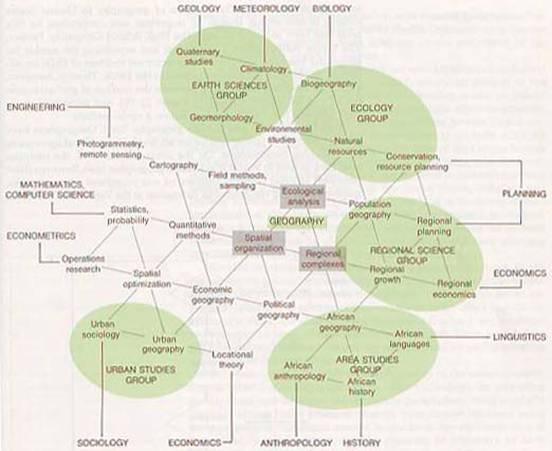
\includegraphics[width=.8\linewidth]{haggett1975_p587.jpg}
    \end{sidecaption}
  \end{figure}

Une exposition des influences de l'écologie, et des sciences naturelles (voir également le schéma plus général proposé par Haggett en 1975 \ref{fig:I_geoLink}), que l'on retrouve beaucoup plus détaillée dans l'étude de l'écologiste et géomorphologue \textcite{Stoddart1967} parue en 1967.

D'un point de vue opérationnel, et c'est aussi le cas dans les précédents ouvrages de ces pionniers, seules des tentatives probabilistes sont évoquées, via les travaux d'Hägerstrand, ou des économistes comme Curry. La méthode hypothético-déductive héritée des premiers géographes théoriciens semble encore être un implicite à la construction et l'évaluation des modèles. Les idées fortes de la systémique semblent avoir été entendues, mais paradoxalement il n'y a à cette période que très peu de référence qui se rapportent aux techniques mathématiques ou informatiques capables d’opérationnaliser un tel système, et aucune application réelle. \autocite[467-468]{Harvey1969}

\paragraph{Les pionniers de l'opérationalisation systémique en Europe}

La génération suivante de géographes va jouer un rôle important dans l'opérationnalisation de ces concepts au début des années 1970, tant en Angleterre, qu'en France où les géographes développent en collaboration avec des mathématiciens et physiciens les aptitudes nécessaires à la manipulation de ces nouvelles techniques computationnelles. \autocite{Pumain2002}

En Angleterre, la planification est issue d'une tradition qui date pour le \textit{Regional Planning and Policy} d'après 1920, et pour le \textit{Land use planning} d'après 1930. Ces activités sont rapidement construites en relation étroite avec les universitaires, les ingénieurs et les politiques publiques \autocites{Bennett2003}[727]{Davies1997}; un existant qui va être bouleversé courant des années 1960-70 par la rencontre conjointe des développements théoriques systémiques, des modèles de planification américains du milieu des années 1950, et d'une littérature qui anticipe la vague systémique. \autocites{Mcloughin1969}[4-8]{McLoughin1985}[253]{Batty1978} \footnote{\foreignquote{english}{The quantitative revolution in geography as encapsulated in books such as Peter Haggett's (1965) Locational Analysis in Human Geography, the various special issues of the Journal of the American Institute of Planners on traffic (1959) and land-use models (1965), books on the post-industrial structure of cities such as Explorations into Urban Structure (1964) all bolstered and anticipated the systems approach. The second edition of Stu Chapin's Urban Land Use Planning in 1965 was also a land mark in the changing conception of planning in America.}}

C'est sur ce substrat \autocite[253]{Batty1978} que des auteurs comme McLoughlin ou Chadwick publient dès le courant des années 1960 des états de l'art et des manuels d'applications qui vont rester pendant presque dix ans des références pour repenser la planification urbaine sous l'angle nouveau de la systémique \autocite[719]{Davies1997}. Une période qualifiée d'âge d'or pour la systémique anglaise, qui même si elle dure peu de temps \autocites[726-727]{Davies1997}{McLoughin1985}, marque toute une jeune génération de planificateurs qui vont être profondément influencés par ces approches \autocite[256]{Batty1978}; un constat alors en complet décalage avec la situation américaine, qui cristallise comme on a pu le voir dans la section \ref{ssec:crise_mutation} l'échec d'une décennie déjà révolue; les nouvelles pratiques, les nouveaux modèles ayant déjà exfiltrés les Etats-Unis, et la nouvelle génération bricolant déjà les meilleurs modèles en vue de les améliorer. C'est dans ce cadre notamment que le physicien et planificateur Wilson publie en 1970, le résultat de 4 ans de travail pour concrétiser son idée, passer du paradigme newtonien au paradigme statistique Boltzmanien pour revisiter dans une version spatiale et dynamique les modèles numériques classiques américains. \autocite{Wilson2010} Une approche qui va devenir avec le temps \enquote{l'école entropique} comme la nomme \textcite{Guermond1984}.

De cette plus jeune génération, à la croisée de ces inspirations, et tout à fait conscients des errements passés \footnote{Voir la conclusion de l'ouvrage de \textcite[357]{Batty1976} ou l'auteur fait le point sur ces différentes positions, toutes abordées en filigrane dans ce livre synthèse : prédiction, explication, éducation }, on trouve des chercheurs maniant parfaitement ces techniques hybrides. Michael Batty est un bon exemple de chercheur représentatif de cette synthèse, qui pressent l'urgence de s'engouffrer dans une modélisation spatialisée plus dynamique \autocite{Batty1971,Batty1972} appuyée par les mathématiques des systèmes dynamiques, que cela soit au travers du vocabulaire de la dynamique des systèmes de Forrester, ou en suivant la toute nouvelle voie des modèles dérivées de l'école entropique de formation par Wilson.

%Le canal en écologie et géographie physique, dans la lignée des travaux de Chorley va également être particulièrement influent, avec l'avénement de modèle opérationel dérivée de la dynamique des populations de Lotka. \autocite{Batty 1971 ou 1972 ....}

%On trouve une analyse des premier essai systémique de Chorley analysé par le prisme des proposition du découpage de Parsons dans l'essai de Gregory.

Comme déjà évoqué brièvement à la fin de la section \ref{sssec:realite_neopositiviste}, les géographes français semblent au début des années 1970 peu réceptifs à l'épistémologie néo-positiviste, et beaucoup plus concentrés sur l'apport des nouvelles méthodes quantitatives dont la substance est révélée brutalement aux géographes français par la lecture (et ensuite la traduction) de manuels anglo-saxons qui condensent déjà 15 ans de pratiques et de découvertes \autocite[129]{Pumain2002}.

Concernant la diffusion du paradigme systémique \footnote{Le cas de la diffusion des méthodes quantitatives en France et de sa structruration en réseau de chercheurs fait actuellement l'objet de la thèse de \textcite{Cuyala2014} dirigé par Marie-Claire Robic, Denise Pumain.}, les recherches d'Olivier Orain \autocite{Orain2001} sur ce sujet sont précieuses. L'auteur nous propose de lister dans les embranchements intellectuels d'une discipline en pleine reconstruction, les convergences et divergences autour de l'acceptation de concepts dont Orain estime qu'ils se sont diffusés dans la géographie française au début des années 1970. La diffusion de la GST de Bertalanffy est renforcée par la publication en 1973 de son ouvrage principal, alors même que l'activité conjointe (publications, traductions, organisations de conférences, d'ateliers) de différents passeurs ayant séjourné à l'étranger comme Bernard Marchand, Wanda Herzog, Henri Reymond, Jean-Bernard Racine, Sylvie Rimbert est soutenue par des acteurs \enquote{installés} comme Philippe Pinchemel, Paul Claval, Roger Brunet, Charles-Pierre Péguy \autocite{Pumain2002,Cauvin2007}, déjà au fait des publications et techniques pionnières anglo-saxonnes.

% NOTE CLEMENTINE et FDD ? il me semble que c’est une des premières thèses françaises dont « système » est le mot clé

Le mot \enquote{système} sort de l'ornière du sens commun et se pare de nouvelles significations, sous l'effet notamment d'ouvrage de référence comme celui de Jean-Bernard Racine et Henri Reymond  \textit{L’Analyse quantitative en géographie} (1973). Premier livre de géographie quantitative en France \autocite{Cauvin2007}, il développe un \enquote{ [...] vibrant plaidoyer pour le développement de concepts et de méthodologies systémistes dans une discipline qui selon eux, \enquote{ découvre que la notion de système lui était depuis longtemps familière, comme la prose à Monsieur Jourdain, et qu'il ne lui manquait que de la formaliser pour la rendre opérationnelle.}} \textcite{Orain2001}. Un appel qui sera entendu semble-t-il, pour Orain \autocite[23]{Orain2001} une des explications pour comprendre le succès connu par la systémique fin des années 1970 début 1980 est le fait que \enquote{[...] les Nouveaux Géographes [...] ont trouvé dans l’idée de système un appareil conceptuel permettant à la fois de penser l’intégration de l’hétérogène et d’apporter une légitimité scientifique à l’étude de la région}

\Anotecontent{etat_artDPMC}{Sur cette thématique on trouve un excellent récit de Denise Pumain et Marie-Claire Robic \autocite{Pumain2002}, ou de Colette Cauvin \autocite{Cauvin2007}}

Dans l'établissement d'une géographie systémique, le Groupe Dupont qui nait à la suite de la conférence \enquote{révélatrice} donnée par Marchand en 1970 s'avère être un creuset important pour la formation, la réflexion, l'échange intra/inter-disciplinaire, et l'expérimentation autour de ces nouvelles techniques \autocites[2]{LeBerre1987}[125-128]{Pumain2002}. Une structure d'accueil que l'on imagine nécessaire pour fédérer des jeunes géographes plus habitués à l'étude monographique qu'à l'utilisation d'outils computationnels. Une période 1971-1975 marquée par la volonté des \enquote{nouveaux géographes} de se former aux mathématiques, une étape absolument nécessaire pour tirer profit par la suite de ces nouveaux formalismes statistiques et informatiques. \Anote{etat_artDPMC}

% REVUES ÉGALEMENT, voir Pumain2012 (quarante glorieuse de l'espace geographique)

En termes de réalisation, différentes écoles vont se créer autour d'objet géographiques ou de techniques parfois différentes, mais avec la même volonté de rendre compte de la complexité des systèmes géographiques en usant des outils mis à disposition par ce nouveau paradigme systémique.

François Durand-Dastès et François Auriac sont des exemples de géographes qui développent dans leurs études toute la puissance heuristique des concepts systémiques et de leur traduction graphique pour décortiquer la complexité des systèmes géographiques.

Un autre groupe de géographes va pousser cette démarche heuristique encore plus loin, en lui donnant corps dans des modèles de simulation. C'est le cas par exemple du projet A.M.O.R.A.L ( Analyse systémique et MOdélisation des ALpes ) réalisé par des géographes et informaticiens Grenoblois, qui est un des premiers résultats d'approche systémique spatialisés ayant pour objet d'étude une région française. Un double enjeu et une double expérience ici pour ces géographes, qui décident de tester la méthode systémique en la déroulant dans sa totalité, ce qui signifie également pour les étapes de réalisation de collaborer avec des informaticiens sur la partie système dynamique. \autocite{Guermond1984, LeBerre1987}

\Anotecontent{exp_amoral}{\enquote{[...] mes premières tentatives de modélisation systémique sont liées à un événement conjoncturel : la rencontre de chercheurs en informatique qui travaillaient, dans l'esprit de la dynamique de système de J.W. Forrester, à la mise au point d'un nouveau langage de simulation. Ils cherchaient à identifier, pour les formaliser, les types de problèmes soulevés par les recherches appliquées. Le groupe de géographes grenoblois avec lequel je travaillais, séduit par quelques ouvrages sur l'approche systémique, était tout prêt à faire l'investissement intellectuel pour tenter son expérimentation en géographie. C'est ainsi que nous avons choisi de modéliser la dynamique de l'emploi dans le système urbain de la région Rhône-Alpes.} \autocite[8]{LeBerre1987}}

Dans le cas du modèle A.M.O.R.A.L \autocite{Durand1983}, la démarche poursuivie est explicitement\Anote{exp_amoral} celle de l'expérimentation de l'\enquote{approche systèmes dynamiques} \autocite{Rosnay1975} à l'étude de la région, avec en tête des modélisateurs la réalisation de multiples objectifs, à la fois d'apprentissage, d'amélioration (prise en compte du spatial), de faisabilité, et d'applicabilité décisionnelle.

\Anotecontent{it_allen}{\enquote{Mais la rencontre opérationnelle - décisive -je l'ai faite en 1982, en allant à Créteil écouter - ne me demandez pas pourquoi - un colloque sur l'entropie dans lequel Peter Allen faisait un exposé sur les théories de l'auto-organisation. Dans cet exposé, il décrivait les modalités de changement de ces systèmes ouverts, loin de l'équilibre, qui connaissent de multiples fluctuations, dont certaines pouvaient s'amplifier et contribuer à modifier la structure du système tout autant que certaines bifurcations externes. C'était exactement ce que j'avais observé en étudiant les recensements périodiques de population, en poids économique, et transformaient leur structure qualitative sur le plan de leur portefeuille d'activités économiques, sur le plan de leur composition sociale, tout ceci en lien, bien sûr, avec des représentations que nous avions de cette dynamique des villes en terme d'images de marque, d'attractivité pour les migrations, etc.
Tout de suite j'ai été séduite par cette approche, et j'ai essayé d'expérimenter avec ces modèles mis au point par Peter Allen, qui à l'époque travaillait encore dans le laboratoire de Prigogine à Bruxelles avec Michèle Sanglier, mais plus particulièrement en direction d'applications à l'économie et à la géographie.[...] Il élaborait en effet des modèles spatialisés, nottament un modèle dynamique intra-urbaine ou intrarégionale [...]; il y'avait là beaucoup d'éléments de théories géographiques qui étaient mis dans un modèle de simulation qui permettait d'expérimenter les effets de ces briques théoriques et de les confronter à des observations.} \autocite[153-154]{Schmid2014}}

\Anotecontent{appli_allen}{\enquote{Tous ces auteurs se sont toutefois heurtés à l'insuffisante prise en compte de la dimension spatiale dans cette famille de modèles. Aussi, des travaux application et élaboration de \textit{modèles urbains} qui soient à la fois \textit{dynamiques et spatiaux} sont en cours. Un modèle comme celui de P.Allen (1978), fondé sur l'analogie des structures dissipatives en physique, permet de simuler le développement d'une ville en tenant compte des interactions non linéaires (avec effets d'amplification ou de saturation), spatiales ou non spatiales, qui commandent la redistribution des emplois et des populations entre les différents quartiers. Il permet de prévoir diverses configurations possibles dans le futur à partir d'une histoire donnée. Ce modèle a été appliqué à la simulation du développement de agglomération de Rouen (Ozan et al. 1983)} \autocite{Pumain1983}}

\Anotecontent{auto_definition}{Un autre concept important est introduit par Ashby dans le mouvement Cybernétique, l'introduction du mot \enquote{auto} amorcent un virage réflexif propre à la seconde Cybernétique, piloté par William Ross Ashby et Von Foerster. Si le concept en lui même est largement intuité dans les thèses de Goethe et Bertalanffy \autocite[102]{Pouvreau2013} dans sa traduction biologique, on retrouve un concept équivalent dans le \enquote{order-from-noise} de Von Foerster, et \enquote{order-from-fluctuation} dans la physique de Prigogine.}

De façon parallèle Denise Pumain, aidée par d'autres géographes comme Lena Sanders et Thérèse Saint-Julien participe dès 1980 d'un courant \autocite{Pumain1983, Pumain1984, Pumain1989} qui vise l'application des modèles de simulation à l'étude des villes et des systèmes de villes, et cela sur des bases beaucoup plus empiriques, devançant ici les diverses tentatives des anglo-saxons faites jusqu'à alors \autocite[99-100]{Pumain1989}. Mais dans le cas de cette équipe, si l’intérêt porté à la dynamique des systèmes de Forrester est là aussi évidente \autocite{Pumain1983, Pumain1984}, le chemin emprunté sur le plan opérationnel va semble t il rapidement diverger de celui suivi par l'équipe AMORAL.

Une fois la révélation d'une opérationalisation possible par l'usage de la \enquote{dynamique des systèmes}, les géographes peuvent donc aller plus loin dans l'exploration du support mathématique sous-jacent, et ainsi mesurer dans l'évolution des \enquote{systèmes dynamiques} vue comme discipline mathématique la possibilité de construire des modèles encore plus proches d'une évolution réelle des objets géographiques.

Ainsi, là où le modèle AMORAL cherche à spatialiser l'approche systémique qui dérive de la dynamique des systèmes de Forrester, les frustrations de l'équipe de Denise Pumain face à leurs propres études passées sur la dynamiques des villes vont les amener à explorer un tout autre chemin en termes d'opérationalisation.

A l'origine ce sont deux conférences qui amènent Denise Pumain à intégrer l'univers systémique à ses analyses, \enquote{la première organisée à Boston au MIT en 1981, encore très largement dominée par l’analyse de systèmes de type Forrester, et la seconde à Bruxelles en 1982 (AFCET, SOGESCI, 1982) déjà largement consacrée aux théories de l’auto-organisation.} \textcite[27]{Pumain2003} \autocites[27]{Pumain2003}{Schmid2014}

\hl{transition ici maladroite}
Mais en réalité, ce n'est pas tant l'évolution des concepts qui comptent pour les géographes mais leur définition en termes opérationnels dans les modèles de simulation \autocite{Pumain2003}, seul moyen de confronter les données récoltées à ces nouvelles formes d'explications mathématiques. Bertalanffy entre autre l'avait déjà bien compris, mobilisées sans réelles démonstrations, les hypothèses intuitées, même lorsqu'elles sont quasi certaines, ne sont tout au mieux pour les autres chercheurs que des aides à la réflexions. Ainsi, et c'est avec une rapidité presque déconcertante, qu'il se raccroche aux premières découvertes de Prigogine en 1946 sur la physique des systèmes ouverts loin de l'équilibre pour appuyer ce qui jusque là ne sont que des intuitions dans sa théorie organismique, et qui forme le prélude à un projet systémique plus général (voir Annexe A pour plus de détail).

Ainsi, et c'est dans ce contexte de frustration par rapport aux approches existantes \Anote{appli_allen} que se produit au début des années 1980 cette découverte contingente du concept d'auto-organisation, dont la réalité opérationnelle exprimés dans des modèles mathématiques exposés par les physiciens de l'école de Bruxelles semble offrir tout à coup toutes les garanties pour former des modèles de simulations beaucoup plus réalistes de l'évolution des villes. \Anote{auto_definition} \autocite[350]{Pumain1998a} La possibilité également de concrétiser les intuitions systémiques des pionniers qui envisagent très tôt la nécessité de penser les systèmes urbains comme des systèmes ouverts, comme celle évoquée en 1964 par \textcite{Berry1964a} et son article \enquote{Cities as systems within systems of cities}. La rencontre de Denise Pumain avec le chimiste  Peter Allen en 1982 à Créteil \Anote{it_allen} est l'expression même de cette contingence, qui va donner par la suite naissance à de multiples modèles et collaborations avec les physiciens de l'école des \enquote{structures dissipatives} de Bruxelles d'abord, puis de l'école de la \enquote{Synergétique} de Haken ensuite. \autocites[27]{Pumain2003}{Pumain1982b, Schmid2014}.

A une phase cybernétique déjà révélatrice de concepts systémiques tout à fait nouveaux pour penser la causalité en géographie, les géographes découvrent par extension la richesse et la pluri-disciplinarité des systèmes dynamiques, alors en pleine évolution. Pourtant déjà évoquée par Poincarré, et étudiée par différents mathématicien dès le début du siècle, la diffusion des théories de la bifurcation n'atteint son point culminant que courant des années 1970. La conférence de New York en 1977 qui se tient sur ce sujet est selon \textcite{Dahan1991} un marqueur singulier de cette dynamique convergente qui pousse de multiples disciplines (physiques, chimiques, biologiques, etc. ) à se rencontrer, non seulement pour evoquer et mettre en commun leurs questionnements et reflexions sur la nature instable des phénomènes, mais aussi pour venir chercher dans cette conférence de nouveaux outils mathématiques adaptés à sa formalisation. L'apparition de \enquote{systèmes frontières} comme par exemple le système de \enquote{Rayleigh-Bénard} va constituer en devenant un objet d'étude partagé, un formidable point de rencontre entre les points de vue originaux des physiciens développant des appareils de mesures, physiciens, thermodynamiciens, hydrodynamiciens. Mais \enquote{l’adoption d’une approche de type système dynamique pour le comprendre ne constitue pas le moteur principal de la convergence. En fait, l’adoption du langage des systèmes dynamiques est ici plutôt la conséquence d’un désir de convergence manifesté par divers groupes de scientifiques} \textcite{Dahan1991}

%\begin{framewithtitle}{Les théories de la bifurcation}

	% \begin{figure}[h]
	% \begin{sidecaption}[fortoc]{Un exemple de bifurcation Pitchfork}[fig:S_BPF]
	%   \centering
	%  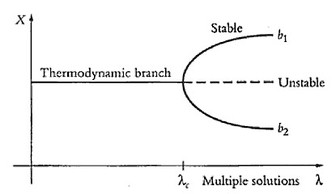
\includegraphics[width=.7\linewidth]{pitchfork_bifurcation.jpeg}
	%   \end{sidecaption}
	% \end{figure}

%\end{framewithtitle}

%La théorie des catastrophe de René Thom, bien connus des géographes, est un cas particulier de la théorie des bifurcations.

Elle offre un support aux découvertes des physiciens engagés depuis les années 30 dans les travaux sur les processus physiques et chimiques des systèmes ouverts éloignés de l'équilibre, qui observe dans la trajectoire d'évolution de ces systèmes l'apparition de zone d'instabilité, causé par la modification en interne des fluctuations ou en réponse à des variations des échanges externes avec l'environnement.

Si certaines conditions d'une auto-organisation avait déjà avancé dans une preuve matérielle ( Homéostat ) et un support théorique (Loi de la Variété requise) dans les travaux par exemple d'Ashby \autocite[800-801]{Pouvreau2013}, les physico-chimistes comme Prigogine ou Haken, en montrant qu'il était possible dans certains systèmes physiques (laser) ou chimiques (structures dissipatives) chaotiques, de voir apparaître au cours des bifurcations de nouveaux équilibres dynamiques caractérisés par l'émergence de structures ordonné de niveau supérieur issue de l'organisation des interactions à un niveau inférieur, ont fournit une évolution du substrat théorique et mathématique solide du concept d'auto-organisation sur lequel peuvent s'appuyer les chercheurs pour expérimenter des analogies dans les systèmes sociaux ou biologiques.

%l'approche d'un point de bifurcation correspondant à l'émergence d'une structure lié à une variation de paramètres dans un processus chaotique/instable décrivant une trajectoire stable entraînant l'émergence imprévisible d'un nouvel état ordonné/stable, dont la structure est maintenu par consommation d'énergie extérieure.

%dévoile de nouvelle perspectives pour penser l’emboîtement et les relation opérant entre les différentes échelles d'observations (voir Annexe A).

%La matérialisation d'un modèle urbain, même théorique, ouvre la voie à des développements qui ouvre la voie à une nouvelle forme de causalité.

La translation de ces concepts sera opérées avec précaution par Pumain et Sanders, et amène une réflexion sur l'évolution des objets géographiques dont on trouve une plus grande explication dans les textes de \textcite{Pumain1982b, Pumain1989}.

%L'apport du paradigme systémique, et de son opérationalisation

%Sous détermination
%Equifinalité

%Les deux approches sont clairement supportés par une double dialectique dans l'utilisation des outils statistiques et systémique, et dans la déduction et l'induction. (hum)

%\enquote{Tenant pour légitime de traiter les êtres vivants et leurs associations comme des systèmes physiques, Lotka insistait toutefois sur le fait qu’il s’agit de « systèmes ouverts » aux flux de matière et d’énergie (ainsi que Raymond Defay (en 1929) et Bertalanffy (en 1932) les qualifièrent plus tard), capables d’échapper à l’équilibre thermodynamique défini par un maximum d’entropie promis aux systèmes fermés par le Second Principe, et d’évoluer vers une structuration croissante.}\autocite{Pouvreau2013}

%\autocite{Pouvreau2013} sa théorie arrive à maturation : \enquote{Un système organique quelconque n'est essentiellement rien d'autre qu'un ordre hiérarchique de processus qui se tiennent mutuellement en équilibre de flux [...] Un organisme vivant est un ordre hiérarchique de systèmes ouverts, qui se maintient sur la base de ses conditions systémiques par un changement de ses composants}

%L'apport de ces techniques, est un vrai écho à ce que disait Le Berre; Sanders et Pumain. D'une part les outils permettent d'ouvrir de nouvelles perspectives de réflexions, et ceux ci s’intègrent dans une chaîne de raisonnement qui s'organisent non pas de façon linéaire mais dans dialogue ou ce sont les usages, les questions, les objets à étudier qui guident l'utilisation et l'amélioration de ces outils.

% Partant de Pumain2002 Pumain2003, la première remise en cause de la causalité est le concept de non linéarité des interactions,

% Relation de variété entre les niveau de hierarchie, augmentation du degré de variété, ce qui va avec le concept équifinalité, un peu different du concept de sous détermination...
% Plusieurs débats qui vont venir agiter la problématique de la construction des modèles, et surtout de leur validation.
% Forrester causalité, construction des modèles, sous détermination
% Auto-organisation problématique de

%Dans cette partie, il s'agit donc de mettre en avant ces débats philosophiques en les reliant aux nouvelles problématiques de construction des modèles tel qu'elle apparaissent aux tournant des années 1970.

%Quel sont les moyens offerts de cette validation ? Existe-il une spécificité de cette validation dans son application en science sociale, et plus spécifiquement en géographie, et qui n'est pas prise en compte dans ces définitions ?

%Plusieurs débats viennent encadrer à la fois la validation mais aussi le support opérationel de cette validation. Autrement dit, comment détermine t on si un modèle est validé ou pas, et quel est la nature de cette validation opère sur un substrat particulier, qui en fait une expérience sur le réel de second ordre.

%IMPORTANT : Necessite d'avoir une validation pour les sciences sociales.

\hl{Transition}


\subsubsection{L'impact du \enquote{programme Forresterien} dans le débat sur la Validation}
\label{sssec:forrester_impact}

Deux dates sont à retenir dans le programme Forresterien, la publication du \enquote{programme} d'\textit{Industrial Dynamics} en 1961; aboutissement des recherches démarrées en 1956 au MIT, et dans un deuxième temps en 1969 la proposition de translation de ce programme à l'étude plus large des systèmes sociaux, avec l'expérience du modèle \textit{Urban Dynamics}.

Pourquoi parle-t-on de programme ici, et non pas seulement de modèle ?

L'apport de Forrester ne se résume pas en réalité au seul nouveau langage de programmation DYNAMO, celui-ci propose aussi avec une méthodologie et un vocabulaire graphique. Trois éléments qui une fois réunis permettent de dériver opérationnellement les concepts clefs du projet systémique dans un modèle de simulation dynamique, ce qui en fait un outil d'intérét général non seulement pour la géographie, mais pour toute les autres disciplines confondues (biologie, économie, sciences humaines, etc.) \autocite{Rosnay1975}

\hl{A muscler pour faire coller avec le reste}

\paragraph{Urban Dynamics, un révélateur des nouveaux usages pour la construction et la validation des modèles ?}
\label{p:urbanDyn_revelateur}

Provenant d'une toute autre inspiration et construit selon un tout autre patron que les modèles urbain réalisé jusqu'à la fin des années 1970, le modèle \textit{Urban Dynamics} de \textcite{Forrester1969} fait une entrée très remarquée dans le milieu des \textit{policies}. Celui met en jeu une ville abstraite et isolée, non-spatialisé, ou interagissent de façon a-spatialisés de multiples mécanismes regroupés par activités et organisés en chaîne causale. Le modèle ne fait appel à aucune donnée pour calibrer ou vérifier les sorties générées, et à ce titre il ne peut pas être considéré comme un modèle décisionnel sérieux pour les \textit{policy analysis} de l'époque. \autocite{Lee1973}. Soumis à une très forte médiatisation, les critiques sur le modèle se font parfois vives tant du côté des citoyens \autocites{Forrester1989, Forrester2007} que des universitaires géographes \autocites{Tobler1970a, Berry1970b, Batty1971, Batty1976} .

Il est vrai que d'un point de vue purement géographique et même technique, le modèle \textit{Urban Dynamics} n'introduit pas tant d'originalité par rapport aux éléments acquis par la rencontre entre la vision d'Hägerstrand et les pionniers universitaires 10 ans auparavant; on se remémorera à ce sujet la citation de \textcite{Morril2005} qui résume très bien l'importance de cette convergence, ici en quatre grands points : \foreignquote{english}{First was the introduction (at least at the geography) of the idea of spatial and time-processes, that geographic development over time could be understood and modeled; second was the particular processes of spatial diffusion; third was the technique of Monte-Carlo simulation; and fourth was the idea that individual behavior, not just that of large groups, could be modelled}. Ainsi après tout, les premiers modèles de simulation qui incorporent la dimension temporelle, stochastique, dans le premier langage Fortran, sont datés d'avant 1965, et dépassent en bien des aspects la vision a-spatiale proposée par Forrester.
\Anotecontent{batty_temps}{Exceptions dont on trouve une liste comparative réalisé par \textcite{Batty1972} incluant entre autre la gestion de l'espace, du temps, et la nature des dynamiques \footnote{Le modèle TOMM (Time Oriented Metropolitan Model) de Crecine, le modèle EMPIRIC, les travaux de Paelinck, ou encore de Wilson qui adapte les travaux existants en démographie, ou hérités de la dynamique des populations en écologie/biologie}}

L'étude des processus de diffusion abordés dans les simulations pionnières suppose assez naturellement que les géographes intègrent le temps dans leurs analyses, et il a été vu précédemment que la simulation est un formidable outil d'expérimentation pour la projection et l'évaluation dans le temps de multiples hypothèses (section \ref{ssec:labo_virtuelle}). En dehors de quelques exceptions \Anote{batty_temps}, pourquoi cette approche percole t elle aussi lentement dans l'analyse des systèmes urbains en géographie, où la simulation numérique est mobilisée à la même période sans pourtant y intégrer la dimension temporelle. Sorte de principe de parcimonie poussé à l'extrême, ou l'absence du temps si elle permet de simplifier l'analyse, mène toutefois à des prédictions absurdes ou impossibles, qui ne tiennent pas compte des évolution de structures sur lesquels s'appuient les interactions dans les systèmes urbains. Le constat d'une forme d'auto-censure de la discipline pour laquelle \textcite[296-297]{Batty1976} nous donne quelques pistes de compréhensions sur lesquelles il nous faudra revenir (\hl{section à appeler}) :

\foreignquote{english}{There are, however, good reasons why the comparative static approach has been widely applied. The status of theory in urban economic and geographic systems with regard to time is almost non-existent. [...] Yet there are severe problems in trying to develop dynamic theory, two of which are worthy of some discussion.[...]

Perhaps the major problem concerns the ability to observe or monitor the urban system. Unlike the physical sciences in which the effect of critical variables on the system of interest can be isolated in the laboratory, such a search for cause and effect is practically impossible in social systems. Thus, there are many instances when it is difficult, if not impossible, to disentangle one cause from another in the changing behaviour of such systems. This is a fundamental limitation which is referred to here as the \textbf{observational dilemma}.

A second problem concerns that hoary perennial data. [...] data are often difficult to assemble for one cross-section in time, and the collection of time series data is usually a formidable and sometimes infeasible undertaking. Furthermore, such data often become less consistent and sparser as earlier time periods are needed and, frequently, the time periods between points at which data have been collected, are too large to be useful for dynamic modelling}

%%NOTE CLEMENTINE à ce propos, pour préparer mon entretien skype, j’ai regardé plein de vidéos récentes de Batty et de son accent bien anglais. Y’en avait une je sais plus où assez cool qui répond à cette citation de 40ans. En gros, il parle des Big Data et de la façon dont leur structure (non-exhaustif, irrégulières dans le temps mais dans un temps plus ou moins continu etc.) change qualitativement les analyses. C’est pas juste plus de données mais données différentes et questions à poser d’un autre ordre. juste comme ça.

Si on revient au modèle \textit{Urban Dynamics} de Forrester, celui ci pourrait après tout passer pour une nouvelle tentative parmi d'autres, car comme Tobler le fait remarquer dans sa critique du modèle : \foreignquote{english}{In other words, it is a classical non-linear deterministic equilibrium model, but of great complexity.} \textcite{Tobler1970a}

Pourquoi Batty en fait il alors régulièrement un modèle pivot dans son argumentation dans l'évolution de la discipline \textcite{Batty1971, Batty1976, Batty2001, Batty2008}, et pourquoi celui ci a t il autant attiré l'attention dans le monde académique ?

Sur ce deuxième point, on a déjà donné un élément de la réponse dans l'introduction de cette partie. Forrester vient ici avec plus qu'un modèle, il vient avec un programme \autocite{Forrester1961} qui embrasse littéralement les concepts de la systémique dans sa branche cybernétique \autocite{Berry1970b}, ce qui permet d'apporter, avec l'intégration du temps, un tout nouveau point de vue sur la planification et la mise en place des politiques publiques. Ainsi malgré ses défaut, \foreignquote{english}{[...] the model is an illustrative first attempt that points the way for others. It is the direction that is important, and Forrester's book may yet prove to be one of the important signposts in the attempt to deal more sensitively and effectively with urban problems.} \autocite{Berry1970b}

L'autre point fort du programme de Forrester est la possibilité d'opérationnaliser des concepts de la systémique tout en maintenant un coût d'accès à la simulation qui parait plus adapté au monde académique des sciences humaines et sociales, et cela entre autre par la mise en place d'une triple entrée en la matière : informatique avec DYNAMO (un langage déjà adapté/simplifié pour réaliser des simulation), mathématique avec les systèmes dynamiques, et graphique avec les diagramme de \enquote{stock and flow}.

%NOTE CLEMENTINE une figure-exemple ?

Pour ces deux raisons, on comprendra donc ici que le monde académique soit plus intéressé par les nouvelles possibilités offertes par l'environnement support du modèle que par le modèle en lui même, qui restera chez les géographes un cas d'utilisation finalement assez peu repris dans des travaux ultérieurs chez les anglo-saxons \autocite[308]{Batty1976}, et chez les français. \hl{(ref)}

Ainsi, ce n'est pas tant sur les aspects temporels que \textcite{Batty2001} en font un modèle en rupture avec son passé, mais sur le débat qu'il soulève du point de vue de la validation.

\foreignquote{english}{Perhaps the clearest model which broke from this tradition and which illustrated distinctly the problems posed by the current generation of models based on complexity was Forrester’s (1969) Urban Dynamics model.}\autocite{Batty2001}

%DEBUT ORTHOGRAPHE EMILIE
\Anotecontent{batty_donnees}{ Un point sur lequel \textcite{Batty1989} semble encore s'accorder dans les années 1980 pour les modèles urbains. Dans un paragraphe intitulé \foreignquote{english}{Data, Data Everywhere and Not a Thought to Think} il écrit d'abord un premier paragraphe sur l'accès à l'information qui s'avère être d'une actualité étonnante quand on le compare au discours plus récent sur les enjeux de l'\textit{openData} \foreignquote{english}{The diffusion of computer technology and the rise of data banks which contain facts and information about individuals across whole arrays of issues in one of the more siniste features of the emerging information society. There is a sense in which computers attract data in that the availability of information systems leads to their rather unselective use.[...] This proliferation of data, and the many banks which now exist; are available only to those who have the power to buy it, or control it; and although there are clearly better data sets available than there were a generation ago to aid our understanding of cities, for example, access to these data is restricted. There is something rather strange about a situation where data can be collected about ourselves \enquote{freely} but then only made available to us at a cost.} Suite à quoi il déclare \foreignquote{english}{Models had always run into data problems, and lack of data, or at least the right kind of data, clearly did influence the development of the field. But lack of data has never really been a central issue, and in any case it is an open question as to whether any of the appropriate data is available now.[...] Thus data availability has never been the key issue in modelling. As Shubik (1979) says: \enquote{Ours is a data-rich and information-poor society}. The real critique of models relates to more substantive issues, to the question which models are able to respond to, not to the data which are available.} Et, si il est évident qu'il existe de nombreuses questions pour lequel il n'existe pas encore de données, cela n'est pas du fait de l'absence de système de collecte, mais bien parce que \foreignquote{english}{Once again there is the obvious point that the useful information can be collected only if some idea of what it is likely to be used for has been established.} }
%FIN ORTHOGRAPHE EMILIE

Pour comprendre la position de Forrester sur ce point il faut s'intéresser d'un peu plus près à sa vision de la modélisation et à l'utilisation qu'il souhaite en faire dans le cadre des politiques publiques. Pour lui, le problème n'est pas tant les données \Anote{batty_donnees}, que l'ont finit toujours par les obtenir, \foreignquote{english}{ [...] but rather inability to perceive the consequences of information we already possess.}. Les gens mobilisent pour l'interprétation des données des modèles mentaux, hors souvent ils se trompent, et les conséquences de leur intuitions amènent alors à constater la faillite des politiques ainsi menées. Pour \textcite{Forrester1971}, l'usage de modèle de simulation permet de re-projeter ces modèles mentaux faillibles sur des modèles informatiques dont la construction nécessite la formulation d'hypothèses de façon plus explicite, plus compréhensible, et sur lequel il est possible de dialoguer de façon plus constructive. Il n'est plus question de choisir en fonction d'un seul scenario, mais de plusieurs, avec la possibilité de projeter et d'évaluer dans le temps les conséquences de dynamiques complexes sur un système simplifié envers un objectif donné, et cela avec la garantie d'une fiabilité bien au delà de ce que le seul esprit humain ne pourrait espérer. Avec souvent un résultat sans appel, \foreignquote{english}{[...] behavior is different from what people have assumed.} Un comportement qu'il arrive à démontrer par le jeu des rétro-actions des mécanismes de son modèle \textit{Urban Dynamics}, qui illustre les effets tout à fait contre-intuitifs de certaines politiques publiques.

Comme sous entendu dans le paragraphe précédent, en réalité on comprend beaucoup mieux la démarche de Forrester dès lors qu'on comprend qu'il n'a jamais été question ici de faire un modèle opérationel, comme le sous tend aussi \autocite{Batty2001} : \foreignquote{english}{It might be, as was argued at the time, that the purpose of this model was to raise the level of debate about the inner city. It was not to provide an operational simulation. It was to foster discussion about possible policy issues.}

Ce qui explique entre autre la curiosité ou la perplexité des planificateurs \autocite{Lee1973} ayant investit des millions de dollars sur plusieurs dizaines d'années dans la construction de modèles s'appuyant sur des récoltes de données à la fois coûteuses et fastidieuses.

Le support de cette discussion passe par l'établissement d'un graphe causal représentatif d'un système clos dans sa définition, mais ouvert dans ses échanges vers l'extérieur, dont les éléments et les interactions entre les éléments sont au centre du débat. \hl{description graphe forrester}

Mais en acceptant cela, et compte tenu de l'\textit{observational dilemna} défini par Batty, le modèle de simulation devient dans l'établissement de sa structure causale la projection d'une histoire, d'un point de vue, ici celui de Forrester et de ses collaborateurs. Dès lors l'attention ne se porte plus seulement sur le résultat, mais aussi sur le bien fondé des hypothèses mobilisées par Forrester pour établir ce résultat.

Il y a un certain paradoxe à voir dans cette situation, car si effectivement Forrester donne à voir avec ce graphe causal son raisonnement, contrairement à de nombreux modèles urbains autrefois qualifiés de \enquote{boîte noires}, c'est précisément sur ce point qu'il va se faire attaquer. Les critiques des géographes ne manquent pas alors de rappeler qu'en dehors de l'a-spatialité et l'isolation du modèle, celui ci n'a intégré absolument aucune référence aux théories urbaines dans son travail. Outre le fait que ce n'est pas très \textit{fair play} de sa part pour les universitaires travaillant sur ce sujet depuis 10 ans, cet isolement relatif (Forrester mobilisera d'autres sources) se traduit dans le modèle par la mise en oeuvre de centaines d'hypothèses (400 équations, 300 variables et paramètres \autocite[63]{Pumain1989}) qui s'avèrent pour la plupart difficilement justifiables ou testables de façon empirique. \autocite[307]{Batty1976}

La critique de \textcite{Tobler1970a} sur ce point est explicite, \textit{Urban Dynamics} \foreignquote{english}{[...] is a classical non-linear deterministic equilibrium model, but of great complexity. Herein lies its importance for it is rather grandiosely conceived. [...] Not only the values of the parameters, but also which variables are chosen for consideration and how they are interconnected, are critical. [...] the danger is that his model has not really been tested empirically, thus the policy implications may be wrong, and the model - because of its complexity - is extremely difficult to test. A very careful study of the many assumptions of the model are required. Also required are more competing models, thus the book’s greatest achievement may be the competition which it stimulates.}

Dernier point, peut être le plus préjudiciable à la démarche vantée par Forrester, est la règle qu'il donne pour définir le choix des hypothèses dans un graphe de causalité : \foreignquote{english}{Formulating a model of a system should start from the question \enquote{Where is the boundary, that encompasses the smallest number of components, within which the dynamic behavior under study is generated?} [...] In concept a feedback system is a closed system. Its dynamic behavior arises within its internal structure. Any action which is essential to the behavior of the model being investigated must be included inside the system boundary.} \autocite{Forrester1968b, Richardson2011}

\Anotecontent{lee_forrester}{\foreignquote{english}{He removed about two-thirds of the model without altering the remaining parts, which were left intact, and the model performance was not significantly altered.}\textcite[176]{Lee1973}}

\Anotecontent{source_amoral}{Le code source du modèle étant disponible dans une seule publication, celle du rapports transmis à la DATAR en 1983 \autocite{AMORAL1983}}

\Anotecontent{batty_forrester}{\foreignquote{english}{An interesting, fruitful and amusing piece of work has been undertaken by \autocite{Stonebraker1972} who has simplified the model drastically by reducing the total number of model equations by two-thirds. The results of running the model in this fashion are much the same as Forrester's and this has led Smith and Sage (1973) to propose the use of hierarchical system theory as a tool for simplifying the model.}\autocite[308]{Batty1976}}

Sachant cela, et le fait que différentes équipes arrivent à reproduire la même dynamique finale avec la mise en œuvre de modèles beaucoup plus parcimonieux, l'effet est catastrophique pour l'argumentation de Forrester ! Lee \Anote{lee_forrester} et Batty\Anote{batty_forrester} font référence en particulier aux travaux de \autocite{Stonebraker1972}.

Ainsi quand \textcite{Batty2001} parlent du modèle de Forrester comme ayant polarisé le débat, ce n'est pour éclairer sa réussite dans cette lourde tâche de fabriquer un modèle crédible sur le plan des hypothèses du point de vue d'une communauté des géographes, car sur ce point l'échec semble complet. Son approche légitime par contre indirectement une construction de modèles complexes qui n'impliquent pas forcément une vérification stricte par les données (sur les hypothèses, mais aussi en sortie). Une \foreignquote{english}{Forrester strategy}, identifiée par \textcite[7-8]{Batty2001} comme le retranchement des modélisateurs dans une rhétorique masquant en réalité une absence de volonté ou une incapacité (technique, méthodologique, philosophique) à justifier de la chaîne causale mise en place dans le modèle, celui ci ne servant plus qu'à animer ou illustrer un débat où clairement la neutralité scientifique n'est plus une priorité.

Le débat s'organise alors autour d'un problème qui parait insoluble, avec d'un côté cette nécessité - pour être crédible d'un point de vue scientifique - de pouvoir justifier empiriquement le réseau d'hypothèses mobilisées dans notre modèle complexe, et d'un autre côté l'impossibilité de pouvoir toutes les justifier du fait de l'\textit{observational dilemna} et de la difficulté/impossibilité d'obtenir des données dans bon nombre de disciplines en sciences sociales. Un paradoxe d'autant plus renforcé quand on sait que la simulation est justement mobilisée dans certaines disciplines pour mettre en valeur des comportements du système jugés inobservables dans la réalité, soit parce que qu'ils ne peuvent pas être isolés, soit parce qu'ils ont tout simplement disparus.

Remis dans son contexte, et bien qu'elle soit affaiblie justement par le choix d'une cible plus politique (une réussite pour avoir montré qu'il y a des phénomènes contre-intuitifs) que scientifique (un échec du point de vue des hypothèses injectées), la thèse de Forrester a le mérite de se positionner comme une validation avant tout dépendante d'un contexte. Un point de vue qui peut paraître évident aujourd'hui mais qui va pour l'époque se heurter à une vision de la validation héritée de l'économie beaucoup plus rigide sur ce point de vue, et dont nous allons voir qu'elle est de toute façon inadaptée à la validation des modèles en sciences sociales.

%Car comment valider un modèle qui ne s'appuie sur aucune données autres que des valeurs de paramètres, et qui évoque des conclusions sans avoir été calibré au préalable ? Comment discuter des résultats de cette longue suite d'hypothèses reliés les uns aux autres par des interaction complexes, difficile ou impossible à vérifier empiriquement ? On retrouve là les deux points évoqués par Batty pour justifier du retard dans l'intégration du temps dans les modèles urbains, sur lesquels Forrester est clairement mis en difficulté.

\paragraph{Forrester, un acteur du débat entre Validation Objectiviste et Relativiste}
\label{p:confrontation_approches}

Avant même la publication de \textit{Urban Dynamics} c'est déjà sa première publication \textit{Industrial Dynamics} qui doit faire face à plusieurs critiques extrêmement vives de la part d'opposants à sa méthode de validation. \autocite{Barlas1990}. Ces derniers affichent alors des vues plus proches d'une autre méthode de validation, beaucoup plus rigide, tel qu'elle est proposée par Naylor; un des pionniers sur cette question et dont la vision a une large influence dans la littérature de la validation courant des années 1960-1970. Un postulat qui se base à la fois sur des commentaires de chercheurs comme \autocite[1088]{Kleindorfer1998} \autocite{Nance2002}, mais également d'une constatation faite dans la lecture des ouvrages collectif \hl{Ref a ajouter}, où Naylor apparaît souvent comme la seule voix référente sur cette question.

Bien que sa méthodologie soit la plus souvent citée dans le domaine de la \textit{V\&V} comme une \enquote{méthodologie historique} \autocite{Sargent2010}, celle ci reste pourtant tout à fait influente et opérationnelle de par sa présence régulière dans des ouvrages d'ingénierie généraliste \footnote{Jerry Banks dans son livre régulièrement réédité \textit{Discrete-Event System Simulation} propose toujours aux lecteurs de valider leur modèle en s'appuyant sur une version synthétique et modernisée de l'approche proposée par Naylor}

Pour \textcite{Kleindorfer1998}, cette vision historique de la validation telle qu'elle a été définie par Naylor est la cause encore aujourd'hui de nombreux malentendus et critiques qui touchent la validation de modèles. A ce titre, et dans le but de faire progresser ce débat, \textcite{Kleindorfer1998} se positionne comme arbitre entre d'un côté l'\enquote{objectivisme} représenté par Naylor, et de l'autre côté la vision opposée plus \enquote{relativiste} représenté par Barlas et Carpenter, eux aussi extrêmement critiques envers la vision de Naylor.

Une fois remise dans son contexte, la méthodologie proposée par Naylor est au premier abord particulièrement intéressante; pas seulement car c'est la première fois que l'on s'intéresse à cette problématique, mais aussi parce que celle-ci aborde cette réflexion en y intégrant spontanément le point de vue de la philosophie des sciences. Mais il ne s'arrête pas là, car c'est avec une certaine ouverture d'esprit qu'il insiste ensuite auprès du lecteur sur la nécessité d'une approche éclectique de cette question de la validation; celle ci n'étant pas pour lui l'histoire d'un seul dogme forcément incomplet, mais d'un faisceau d'approches résolument complémentaires. Il retient trois approches qu'il regroupe par ordre d'application dans une méthode nommée \textit{Multi Stage Validation} et qui contient : le rationalisme cartésien, l'empirisme, et la \textit{positive economics} de Friedman.

Seulement, après lecture et analyse de cet article, on s'aperçoit que les trois points de vues qu'il présente se rapportent à une vision de la validation en réalité assez rigide, comme en témoigne cette citation tirée de l'article de \textcite{Naylor1967} : \foreignquote{english}{To verify or validate any kind of model (e.g management science models) means to prove the model to be true. But to prove that a model is \enquote{true} implies (1) that we have established a set of criteria for differentiating between those models which are \enquote{true} and those which are not \enquote{ true }, and (2) that we have the possibility to apply these criteria to any given models}

Pour \textcite{Barlas1990, Barlas1996}, il existe deux camps philosophiques opposés, et pour lui Naylor fait clairement partie de la première école : \foreignquote{english}{The traditional reductionist logica1 positivist school (including empiricism, rationalism, verificationism and the “strong” falsificationism) would see a valid model as an objective representation of a real system. The model can be either “correct” or “incorrect”; once the model confronts the empirical facts, its truth or falsehood would be automatically revealed. In this philosophy, validity is seen as a matter of accuracy, rather than usefulness. The opposing school (including more recent relativistic, holistic and pragmatist philosophies), in contrast, would see a valid model as one of many possible ways of describing a real situation. \enquote{No particular representation is superior to others in any absolute sense, although one could prove to be more effective. No model can claim absolute objectivity, for every model carries in it the modeler’s worldview. Models are not true or false, but lie on a continuum of usefulness.} \autocite{Barlas1990}.}

\textcite{Barlas1990} fait de Forrester le premier défenseur d'une validation plus en accord avec la deuxième école, une méthode selon lui plus adaptée à l'explication de processus complexes, comme en témoigne ces quelques extraits tirés de son article :

\foreignquote{english}{The first exposition of the system dynamics paradigm as it relates to model validity was given in Chapter 13 of Industrial Dynamics (1961) by Jay Forrester. [...]

Forrester also criticizes the illusion that using fixed statistical significance levels brings objectivity to the validation procedure. [...]

He makes the stronger claim that \foreignquote{english}{the validity of a model should not be separated from the validity and the feasibility of the goals themselves.} Since reaching an agreement on the feasibility of the goals cannot be achieved through a formal algorithmic process, validation becomes very much a matter of social discussion. [...]

Another nontraditional view of Forrester is his willingness to accept \foreignquote{english}{qualitative} model validation. He argues that a negative attitude toward qualitative validation procedures is not justifiable, since \foreignquote{english}{a preponderant amount of human knowledge is in nonquantitative form} \autocite[128]{Forrester1961}. [...]

Finally, Forrester sees explanatory power as being at least as important as predictive power in model validation. Forrester’s views on model validity correspond to the relativist/holistic philosophy of science. }\autocite{Barlas1990}

En ce sens il prend le contrepied de la dernière méthode qui clôt la \textit{multistage validation} de Naylor. La \textit{positive economics} dictée par Friedman, une forme d'instrumentalisme, est complétée par les deux méthodes précédentes (empirisme, rationalisme) pour assurer que la validation du modèle, et des hypothèses qu'il contient, est bien dirigée en priorité par la prédiction : \foreignquote{english}{ Hence the final decision concerning the validity of the model must be based on its predictions.} \autocite[97]{Naylor1967} Or il a été montré précédemment (voir \ref{p:echec_critiques} que c'est bien un des points reprochés par une partie des géographes radicaux que de voir s'aligner une partie des géographes (volontairement ou involontairement) sur une forme d'instrumentalisme, hérité de l'économie, et cela même appuyé par une position empiriste pour la validation des hypothèses.

Clairement le paradigme systémique permet d'échapper à ce discrédit par l'intégration dans les modèles géographiques d'une réflexion à la fois multi-échelle, et multi-temporelle \autocite{Dastes2001a} dont la discrétisation en une multitudes de points d’arrêts pertinents constitue il me semble un appel implicite à l'étude inter-disciplinaire des objets géographiques, et dont la collection est toujours abordée en fonction de la question qui est posée. Ainsi l'étude de l'évolution comparées des systèmes de villes dans le temps long, ou l'étude des mobilités des individus liés à l'attribution des cartes scolaires sont deux exemples de sujets dont les composantes complexes ne peuvent être abordés sans faire appel à l'expertise comparés de sociologues, d'archéologues, d'économistes, etc. qui disposent pour le même objet (l'individu, la ville) de points de vues prompts à enrichir les modèles d'une hétérogénéité permises par la systémique.

Autre point qui semble en divergence avec les pratiques des géographes, la position empiriste de Naylor implique de limiter le choix d'hypothèses mobilisées dans les modèles aux seules qui peuvent être validées par des données : \foreignquote{english}{A simulation model, the validity of which has not been ascertained by empirical observation, may prove to be of interest for expository or pedagogical purposes, but such a model contributes nothing to the understanding of the system being simulated} \autocite{Naylor1967}

Une vision radicale qui se heurte au problème de l'induction comme il avait déjà été évoqué pour les positivistes logiques ( section \ref{p:critique_debat} ), l'accumulation de confirmation n'étant en aucun cas une condition suffisante à la validation d'une hypothèse.

De plus toutes les disciplines n'ont pas la possibilité de disposer de données utilisables pour vérification des hypothèses, et d'autres part la collecte et la structuration des données tient d'un processus qui contient là aussi une part de subjectivité qui rend impossible la mise en place d'un seul jeu d'observation pour validation d'une seule et même hypothèse.

Enfin, cette vision est de toute façon peu compatible avec une étude de la complexité des systèmes sociaux (\enquote{observational dilemna} de Batty), car comment rendre compte par une récolte de données de processus dont on sait d'une part que la perception et donc l'établissement de mesure est subjective (voir point précédent) et d'autre part que ces processus ne peuvent être réduits à leur seule composante du fait de leur intrication dans un réseau complexe d'interaction (le tout est plus que la somme des parties).

%Cela pour plusieurs raisons qui tiennent à la construction des connaissances dans la simulation des systèmes sociaux, dont on verra par la suite qu'elle ne peut que difficilement être similaire à la construction des connaissances dans les sciences naturelles.

%La où la validation proposée par Naylor ne se réalise en effet qu'à l'aune des données disponibles, et se rapproche dans sa description plus d'un résultat binaire propre au cadre d'évaluation des positivistes logiques; Forrester propose avec l'établissement d'un graphe causal l'intégration explicite du social, du contexte dans lequel se construit, et donc se valide le modèle.

Toutefois, et avant de rejeter l'une ou l'autre approche de façon hâtive, on citera \textcite{Kleindorfer1998} pour résumer quels sont les conséquences pour le raisonnement d'un modélisateur qui veut s'en tenir à la stricte application d'un de ces deux pôles. Ainsi un objectiviste extrême \foreignquote{english}{[...] believes that model validation can be divorced from the model builder and its context. He or she maintains that models are either valid or invalid, and that validation is an algorithmic process which is not open to interpretation or debate.} alors que par contraste un relativiste extrême \foreignquote{english}{[...] believes that the model and model builder are inseparable. As such, all models are equally valid or invalid and model validity is a matter of opinion.}

Évidemment intenables en tant que tels, ces extrêmes portent en chacun d'eux une part de vrai qui les rendent tout deux intéressants. Pour \textcite{Kleindorfer1998} en réalité la plupart des scientifiques intègrent spontanément l'une et l'autre de ces approches dans leurs pratiques de validation.

\foreignquote{english}{Objectivism seeks a common framework with which to evaluate and compare models and a sense in which the validation process transcends the model builders and users. By contrast, the relativist position highlights the need for a dialogue between the model builder and other model stakeholders. According to \autocite{Barlas1990}, validation is \enquote{a matter of social conversation rather than objective confrontation.} We would argue that most practitioners have instinctively adopted a middle ground in this debate.} \autocite[1098]{Kleindorfer1998}

Attention donc ici à ne pas se tromper de cible, \textcite[188]{Barlas1996} en lui même ne rejette pas les méthodes quantitatives, pas plus que Forrester, seulement ils mettent en avant le fait que la procédure de validation ne peut se limiter à une validation totalement objective, universelle, quasi-algorithmique et blâment le fait qu'on puisse penser l'explication au seul terme des prédictions qu'elles sont susceptibles d'apporter.

% REVOIR TRANSITION
%Dès lors on est en mesure de poser la question suivante, quels sont les modalités de cette nouvelle forme de validation proposés par Forrester ?

%PEUT VENIR EN SOUTIENT DE LARGUMENTATION, EN EXEMPLE.
%\paragraph{Forrester, ou les moyens de cette discussion}
% PERMET DE FAIRE EMERGER UN GRAPHE CAUSAL
% PERMET DE FAIRE EMERGER L'IMPORTANCE DU COLLECTIF

%En cela il répond déjà à une des critiques majeures faites aux anciens modèles, composés

% problématique de la tension entre l'objet construit, et l'objet à valider, car la validation on va le voir est le propre à la fois d'une discussion interne mais également externe avec le reste du monde. (du coup il faut aussi développer les moyens, et ca sera la la transition dans la conclusion)

Bien que reconnu comme pionnier, l'approche de Naylor n'est pourtant pas la seule à émerger dans le courant des années 1960-70 \autocite{Balci1980}, ainsi on a vu par le biais de \autocite{Barlas1990} que Forrester disposait déjà en 1961 d'un avis suffisamment tranché pour s'opposer à cette dernière. En étudiant les textes de \textcite{Hermann1967}, on découvre un autre pionnier de la \enquote{V\&V}, opérant cette fois ci dans un tout autre contexte de modélisation que Naylor. On se rend compte que le discours développé par Hermann est d'une toute autre nature; tout en étant compatible avec le discours de Forrester sur la nature contextuelle de la validation, celui ci va plus loin en proposant à la fois une réflexion et des solutions - dont une large partie a été intégrée dans les synthèses successives et ultérieures du mouvement de la \enquote{V\&V} - sur des problématiques qui résonnent encore, à la mesure de nos travaux actuels, comme étonnamment contemporaines.



\subsection{De la Validation à la construction des modèles de simulation par l'évaluation}
\label{ssec:evaluation_construction}

% Permanence des questions évoqués pour la construction d'un modèle de simulation, plus complexification de la validation liés à la pluriformalisation.

En montrant que la validation est dépendante au contexte, Hermann a permis de lever un certain nombre de questions remarquables par leur actualité dans le cadre de nos propres problématiques de construction.  %La mise en avant d'une possibilité de validation dépendante à l'objectif nous oblige inévitablement à prendre en compte l'activité de construction comme activité validante.

\subsubsection{Des modalités de validation dépendantes du contexte, l'apport d'Hermann à une première formalisation du problème}
\label{sssec:hermann_contexte}

\paragraph{Une vision de la validation différente chez les pionniers du mouvement S\&G (Simulation \& Gaming)}

Charles F. Hermann opère dans la branche des simulations appelées à l'époque par Shubik les \textit{Man-Machine Games} \autocite{Shubik1972}. Une catégorie de simulation qui intègre dans son exécution un couplage entre un ou plusieurs systèmes numériques et des humains, qui peuvent être amenés à interagir entre eux, ou avec les machines. Ce type de simulation de structure hétérogène est intéressante dans le sens où elle permet d'intégrer l'arbitraire humain dans une chaîne d'interaction complexe qui n'aurait pas pu être établie autrement, du fait de l'impossibilité de programmer des interactions et des réactions humaines face à des situations précises. Même si ce type de techniques est motivé par une multitude d'usages, ce n'est pas par hasard si elle se développe particulièrement au cours de la guerre froide aux Etats-Unis, toujours sous la direction d'institutions militaires. Ce genre de techniques permettant par exemple de simuler et de reproduire des guerres au travers d'inter-relations diplomatiques et/ou économiques \autocite{Hermann1967b}, avec la possibilité de mesurer via des indicateurs adaptés l'importance et l'impact de différents scénarii sur le couple humain/machine.

Ce type de simulation est particulièrement représenté dans des publications qui traitent de la simulation au sens large, comme par exemple le journal \textit{Simulation and Gaming} ou \textit{S\&G} \autocite{Crookall2011}, dont l'activité remonte au début des années 1970. On retrouve parmi les auteurs ayant participé au développement de la discipline des personnalités importantes comme Guetzkow, Shubik, Coleman, etc. \autocite{Crookall2012}. Aujourd'hui, le terme à évolué vers ce que l'on pourrait probablement appeler des jeux sérieux, l'utilisation de l'ordinateur n'étant plus forcément un élément obligatoire dans ce type de simulation. Du côté des objectifs qui sont aujourd'hui susceptibles de motiver l'utilisation de ces techniques, \textcite{Shubik2009} définit une taxonomie en 6 objectifs : \textit{teaching, experimentation, entertainment, therapy and diagnosis, operations, training }

Cette présence d'une dimension humaine dans les simulations introduit une complexité qui touche forcément à plusieurs objets d'étude des sciences humaines (psychologie, sociologie, etc.), et il n'est donc pas étonnant que l'on retrouve ce type de publication dès l'apparition des premiers ouvrages inter-disciplinaires sur la simulation, quand elle ne les pilote pas; Harold Guetzkow par exemple est un des personnages importants qui gravitent autour de Herbert Simon au GSIA (Graduate School of Industrial Administration) de Carnegie Tech dans les années 1950-56 \autocite{Guetzkow2004}, et qui a beaucoup oeuvré pour le développement de la simulation dans ces sciences politiques et psychologiques (\textit{Inter-Nation simulation laboratory}) \autocite{Janda2011, Druckman2010}. Celui-ci s'inscrit exactement dans la même branche que Hermann, et apparaît deux fois comme premier éditeur dans des recueils de textes pluri-disciplinaires traitant de la simulation au sens large, preuve aussi de son implication dans le développement et la diffusion de ces techniques au-delà de sa propre discipline \autocite{Guetzkow1962, Guetzkow1972}

\paragraph{L'apport du contexte dans l'évolution du sens attaché à l'activité de simulation}

Ce qui est intéressant dans ce type de simulation, c'est qu'elles forcent à penser la validation des modèles sous un angle qui doit nécessairement tenir compte de la variabilité inhérente aux comportements humains, par essence difficilement évaluables et réplicables. C'est de cette contrainte, et parce que \textcite{Hermann1967} s'intéresse aux modèles de simulation pour d'autres objectifs que la prédiction (\textit{teaching, training, theory-building}), que celui-ci développe à mon sens une vision de la validation beaucoup plus réaliste pour les sciences sociales que celle proposée à la même période par Naylor.

\foreignblockquote{english}[{\cite[217]{Hermann1967}}]{First, the validity of an operating system is affected by the purpose or use for which the game or simulation is constructed [...]}

% Plus d'information à ajouter, soit sur la dite boucle (sachant que le conceptual correspond quand meme pas mal à ce que lon fait, voir Sargent2010), Si la boucle définit par les tenants de la \textit{V\&V} n'est pas inintéressante, et de façon générale résume bien le cycle de vie qui correspond à la construction d'une simulation, de nombreuses questions reste en suspens sur le choix et la mise en œuvre des techniques telles qu'elles sont décrites. La construction et la mise en oeuvre des critères en fait partie. Les objectifs sont cités dans la définitions mais on ne rentre pourtant pas dans le détail de la relation entre ces objectifs et la construction du modèle, qui est laissé à l'expertise de l'utilisateur, en cela Hermann ne propose pas mieux dans sa description d'une boucle modélisatrice que les dernières avancées portés par Sargent2010, toutefois sa réflexion est par son orientation, et par sa précocité de réflexion son intéressante il me semble à citer. les moyens technique de la mise en oeuvre par exemple ?

%Dans l'explication sociologique, la réalité structurelle n'est pas forcément d'intérét pour la construction du modèle. (bulle)

%Cette observation amène Hermann à considérer que la validation des composantes de la structure mérite une attention tout aussi importante que la seule comparaison avec des données de sorties, notamment dans un cadre explicatif.  curl -k -o ~/backups/pinboard-backups/pinboard-$(date +\%y\%m\%d).json 'https://api.pinboard.in/v1/posts/all?&auth_token=username:APItokenhere&format=json'

En s'appuyant sur ce premier argument évoquant l'existence d'une dépendance liant processus de validation et objectif poursuivi par le modélisateur, Hermann semble \textit{de facto} mettre en défaut une définition de la simulation ayant comme première et unique vocation de représenter au mieux le système observé. Les modalités de la validation étant maintenant définies par rapport au contexte, la possibilité d'un critère unique pour juger de la validation de façon universelle paraît tout à fait improbable. Afin de montrer qu'il ne s'agit pas seulement d'une question de disponibilités des données, et pour amener par la suite sa proposition de méthode multi-critères, Hermann s'attaque donc en premier lieu à réduire la portée des confirmations apportées sur un système observé par l'emploi de la seule technique de validation basée sur la comparaison de données en sortie des modèles de simulation.

Pour montrer qu'il existe des limitations dans la confiance que l'on peut mettre dans la validation lorsqu'il s'agit de comparer des données historiques (dans le cas des simulations de reproduction de guerre, on parle ici plutôt de reproduire des séries d'événements historiques) - cela même si elles sont idéalement toutes rendues disponibles - aux données en sortie de simulation, \textcite{Hermann1967b} s'appuient sur les travaux de \textcite{Pool1965}.

\foreignblockquote{english}[\cite{Pool1965}]{This correspondence does not demonstrate that the simulation correctly represents the structure and processes that were operative in the historical occurence. We are speculating on the similarity between the historical and simulated inputs on the basis of the similarity of their outputs. Different relationships among various combination of properties in the simulation conceivably could produce outcomes like those in the historical situation.

A simulation of the 1960 national Presidential election predicted the percentage of the vote for each candidate - the outcome - with considerable success. The designers of that simulation observe, however, that \enquote{it may legitimaly be asked what in the equations accounted for this success, and whether there were parts of the equations in the simulation that contributed nothing or even did harm} Further analysis of the equations in the simulation revealed that the outcome was predicted despite the fact that at least one equation misrepresented aspects of voter turnout. Part of the structure was incorrect, but the simulated result still matched the actual outcome. Despite this difficulty, our confidence that the simulation has captured some aspects of the voting process is greater than it would have been if the simulation had failed to replicate the campaign outcome. Confidence in the simulation would increase further as the operating model demonstrated ability to produce outcomes that corresponded with various elections. In sum, the similarity between simulation and historical events can provide at best only indirect and partial evidence for the correctness of the simulated structures and processes that produced the outcome.}

Ce que nous dit Hermann ici, à la différence de Naylor, c'est que même dans le cas idéal où toutes les données seraient présentes, ce mode classique de validation ne peut pas être suffisant, cela quel que soit l'objectif poursuivi par le modélisateur. Un constat que nous avions déjà acquis à la lecture des déboires des géographes avec les préceptes de validation néo-positivistes, associant dans une démarche de modélisation instrumentaliste prédiction et explication (section \ref{sssec:realite_neopositiviste}).

Ce constat reste encore valide aujourd'hui, car comme le rappelle très justement \textcite[32]{Bulle2005}, \enquote{ les problèmes posés en sciences humaines visent cependant, en général, la compréhension des phénomènes. Dans cette optique, l’objet premier de la modélisation n’est pas de faire \enquote{coïncider} les modèles construits avec la réalité qui est celle des effets. Le test par la prévision ne peut assurer des qualités explicatives des modèles.}

Un point de vue partagé par \textcite[106]{Amblard2006}, pour qui \enquote{[...] la recherche de similitudes avec les données, si elle peut être utile, ne peut absolument pas être un critère unique et définitif de validation}.

Autre point important, l'existence de multiples objectifs de modélisation permet à Hermann certes de révéler la diversité et l'attachement de la validation à un contexte, mais surtout de noter d'une part comment la variation de ce dernier affecte les modalités de cette comparaison entre système simulé et système observé, et d'autre part comment cela affecte la perception du résultat engendré par cette comparaison.

\foreignblockquote{english}[{\cite[219]{Hermann1967}}]{The first comment is that the validation of an operating model cannot be separated from the purpose for which it is designed and used. [...] The second observation somewhat mediates the first. For the most part the various purposes for conducting games and simulations do not negate the need for criteria we can use to estimate the degree of fidelity with which one system (the operating model) reproduces aspects of another (the reference system). Given some purposes for using games and simulations (such as exploring nonexistent universes), finding appropriate criteria in the referent system is quite difficult. With other objectives, the value of the operating model may remain even if the fit between the model and various criteria representing the observable universe is poor (as in theory building).}

Indirectement, on observe ici le transfert d'une définition de la simulation comme simple \enquote{type de modèle} vers la définition plus générale d'une simulation \enquote{caractérisée non pas tant par l’unité d’une fonction cognitive qu’elle assurerait toujours sous une forme ou sous une autre que par son fonctionnement interne, fonctionnement qui, bien sûr, mais seulement secondairement, se trouve avoir aussi des conséquences sur sa ou ses fonctions cognitives. Une simulation nous paraît ainsi devoir être prioritairement caractérisée par ce qu’elle est – ou fait – de manière interne plutôt que par ce qu’elle fait au sens d’une fonction cognitive quelconque qu’elle assurerait toujours et qu’on en attendrait prioritairement de l’extérieur : à ce titre, nous proposons de dire qu’\textit{elle est avant tout un traitement spécifique sur des symboles et qui prend toujours la forme d'au moins deux phases distinctes. 1) une phase opératoire [...] 2) une phase d'observation [...]}} \autocite[33-34]{Varenne2013b}

Un point de vue que l'on imagine volontiers partagé par Hermann, lorsque ce dernier propose de questionner la structure interne des modèles dès la première brique posée :

\foreignblockquote{english}[{\cite[226]{Hermann1967}}]{Because \enquote{a complex model can predict real-world outcomes correctly and yet be wrong in many details} \autocite[64]{Pool1965} an investigator may wish to pursue validity approaches which focus on the internal structure of the model at an earlier stage in the operation of the simulation.} 

Suivant ces conseils, si Forrester avait appliqué lors de la construction de son modèle \textit{Urban Dynamics} des analyses de sensibilités (voir le type de critère \textit{variable-parameter testing} de \autocite{Hermann1967}) tel que le propose Hermann, il aurait probablement conclu, comme ont pu faire ces détracteurs par la suite, à l'inutilité d'une bonne partie des hypothèses intégrées dans son modèle, qui s'avèrent en réalité très peu influentes sur la dynamique observée en sortie des simulations.

\paragraph{La nécessité de repenser la représentativité des modèles}
\label{p:repenser la representativite}

La V\&V a toujours mis en avant le fait que la modélisation soit un processus incrémental tout à fait nécessaire pour obtenir un modèle de simulation satisfaisant, que cela soit dans les analyses de Naylor, ou d'Hermann. Ce dernier se réfère dès 1967 au principe de parcimonie, une méthode qui implique une abstraction, une simplification du système à représenter, et qui pour lui met logiquement et automatiquement en péril la représentativité\interfootnotelinepenalty=10000\Anote{Herman_parcimonie}.

\interfootnotelinepenalty=5000

%Une parcimonie hérité du principe d'Ockham dont on sait qu'elle n'est en aucun cas un synonyme de simplicité dans sa mise en oeuvre, celle-ci nécessitant au contraire un effort intellectuel important pour déterminer quelles sont les hypothèses réellement représentatives du problèmes à analyser. %Sur le plan de complexité, Poincarré ou le prix nobel d'économie Herbert Simon à fait état plusieurs fois des capacités d'expression du complexe rendu possible par l'usage de la simulation, et cela même avec des modèles simples.\autocite{Banos2013a}

%Une description de la construction des modèles qui coincide avec ce qui a été dit auparavant sur l'importance de la nature de l'objectif poursuivie sur la perception de cette \enquote{représentativité}, et le fait que cette dernière ne fasse pas systématiquement la valeur du modèle - tant soit peu qu'on arrive à fixer une valeur -

Dans ce que l'on comprend de l'analyse d'Hermann, la perte de représentativité attendue d'un modèle de simulation qui n'est plus strictement dirigé vers la prédiction est compensée par un gain relatif à l'objectif poursuivi qui change la nature de la validation attendue : détection d'alternatives à un comportement, mise en avant de processus simplifiés pour l'éducation, construction de théorie, etc.

Il est donc logique de voir Hermann proposer dans la suite de son analyse de repenser la notion de représentativité et la notion de validation au regard de l'objectif poursuivi par le modélisateur. Il en résulte la généralisation de cette activité de validation dont le résultat se dessine à présent sous le couvert d'un objectif et dans le jeu d'une confrontation entre deux représentations, deux construits prenant pour cible le système modélisé et le système observé.

\foreignblockquote{english}[{\cite[216]{Hermann1967}}]{A simulation or game is the partial representation of some independent system. Usually we are interested in simulation as a means for increasing our understanding of the system it is intended to copy. Therefore, the representativeness of a simulation or game becomes extremely important in assessing its value. The process of determining how well one system replicates properties of some other system is called validation.[...] In the present analysis however, validation will be defined more broadly as any comparison between the representation of a system and specified criteria.}

\subsubsection{Le problème de la Validation ramené à une confrontation des représentations entre système modélisé et système observé}
\label{sssec:confrontation_sysmodelise_sysobserve}

%\hl{repetition ?}
%La question de la représentativité d'une simulation est un sujet délicat à traiter car sa valeur se dessine à l'intersection d'au moins deux activités, la construction d'un modèle opérationel et la construction d'une grille d'évaluation, deux activités dont on s'apercoit par la suite qu'elles sont en réalité étroitement liées.

\paragraph{Quelles hypothèses pour quelle représentativité ?}
\label{p:hypothese_representativite}

Si cette \enquote{représentativité} ne semble plus intervenir dans la valeur du modèle que sous une forme beaucoup plus partielle, quelle est la part de représentativité acceptable que l'on peut attendre pour qu'une hypothèse soit considérée comme explicative ? Autrement dit quelles sont les modalités qui guident l'introduction maitrisée d'une part d'empirie dans un modèle, par l'existence d'un seuil caractérisant le potentiel de représentativité à atteindre pour chaque hypothèse ? Pour l'ensemble du modèle ?

L'acceptation d'un gradient de valeur pour juger de la validation rompt avec la méthode \enquote{binaire} proposée par Naylor, la validation d'un modèle passant à présent par l'acceptation subjective d'un seuil de représentativité relatif à l'objectif poursuivi. Avec pour conséquence notable qu'une \foreignquote{english}{[...] simulation or game relatively valid for one objective may be not be equally valid for another.}

Si la notion de seuil n'est pas explicitement abordée par Hermann, c'est pourtant sous cette acceptation que la \textit{V\&V} actuelle va reprendre ce concept. Avec la position suivante, celui de se fixer un seuil de représentativité général à atteindre \textit{a priori}.

\foreignquote{english}{\textbf{Principle 2: The outcome of simulation model VV\&T should not be considered as a binary variable where the model is absolutely correct or absolutely incorrect } [...] The outcome of model VV\&T should be considered as a degree of credibility on a scale from 0 to 100, where 0 represents absolutely incorrect and 100 represents absolutely correct.

\textbf{Principle 3: A simulation model is built with respect to the study objectives and its credibility is judged with respect to those objectives } [...] The study objectives dictate how representative the model should be. Sometimes, 60\% representation accuracy may be sufficient; sometimes, 95\% accuracy may be required depending on the importance of the decisions that will be made based on the simulation results. Therefore, model credibility must be judged with respect to the study objectives.}\autocite[15-16]{Balci1998}

La position de \textcite[166]{Sargent2010}, tout en étant relativement similaire, propose une vision plus fine et plus réaliste où le seuil de précision attendu est attaché aux variables de sorties.

\foreignblockquote{english}[{\cite[166]{Sargent2010}}]{A model should be developed for a specific purpose (or application) and its validity determined with respect to that purpose.[...] A model is considered valid for a set of experimental conditions if the model’s accuracy is within its acceptable range, which is the amount of accuracy required for the model’s intended purpose. This usually requires that the model’s output variables of interest (i.e., the model variables used in answering the questions that the model is being developed to answer) be identified and that their required amount of accuracy be specified. The amount of accuracy required should be specified prior to starting the development of the model or very early in the model development process.}

Ces deux citations permettent de montrer au passage comment la vision de la validation défendue par Hermann a été intégrée dans une forme très approchante par des acteurs de la \textit{V\&V} comme Balci ou Sargent, dont on a vu précédemment les définitions dans la section \ref{sssec:def_generique_validation}. Ces deux derniers sont en réalité les acteurs majeurs d'une synthèse (voir la figure \ref{fig:S_syntheseBalci}) opérée dans les années 1980-1990 \autocite{Nance2002}, dont on peut dire qu'elle est marquée par un retour à une certaine forme de neutralité (voir par exemple le rejet des aspects philosophiques décrits dans la section \ref{sssec:def_generique_validation} qui se double d'un jargon technique spécifique à l'établissement d'un processus qualité exploitable pour l'ingénierie). Des adaptations qui permettent probablement de mieux accepter en son sein des typologies de techniques aussi différentes que celles de Naylor\interfootnotelinepenalty=10000\Anote{naylor_etonnement} ou Hermann. Régulièrement révisées, \textcite{Balci1998} fait ainsi état dans sa dernière taxonomie d'un catalogue de $75$ techniques différentes dans lequel peuvent piocher les modélisateurs en fonction de leurs besoins.

\begin{figure}[htbp]
\begin{sidecaption}[Synthèse des techniques de Validation par Balci dans les années 1980]{On remarquera la forte présence des techniques présentées par Hermann dans la synthèse proposée par Balci en 1986 \autocite{Balci1986}}[fig:S_syntheseBalci]
  \centering
 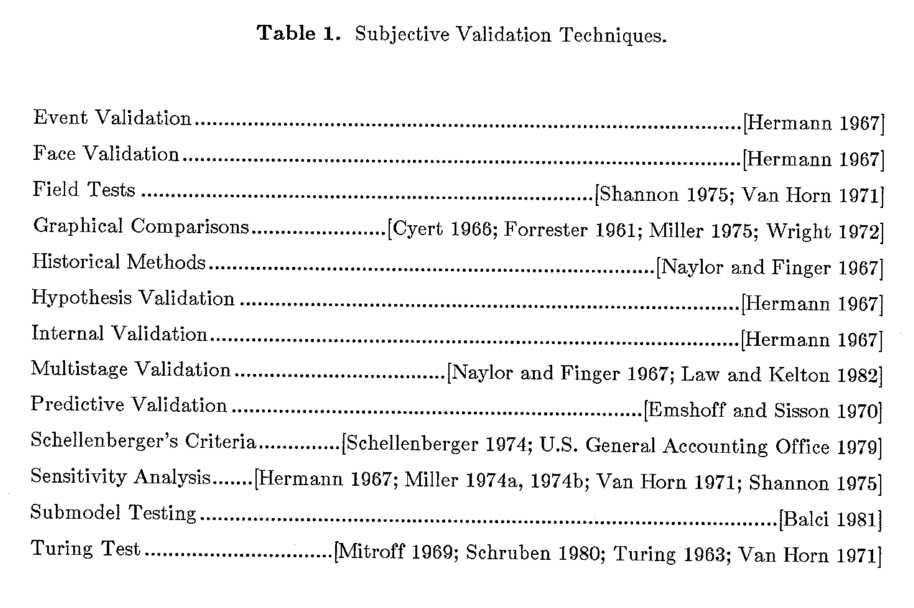
\includegraphics[width=.9\linewidth]{subjective_balci.png}
  \end{sidecaption}
\end{figure}

On se rend bien compte que dans le cadre des sciences humaines et sociales la possibilité de fixer par avance ce type de seuil n'a pas de sens, surtout dans un cadre explicatif.

%\textit{Que faut il entendre ici par partiellement ? Quels sont les leviers permettant au géographe de compenser cette perte de représentativité par un gain en compréhension sur le système à étudier ? }

Pour mieux comprendre quel est l'enjeu de cette délimitation entre un modèle réaliste et un modèle abstrait, il faut évoquer cette tension permanente qui nourrit les choix du modélisateur dans la construction d'un modèle explicatif. Deux attracteurs possibles et apparemment opposés, avec d'une part la volonté de se rattacher à une forme de réalisme au travers de l'injection d'une part maîtrisée de réalité tout au long du processus de construction\Anote{durand_observation}, et d'autre part une force qui nous pousse au contraire à se détacher de cette même empirie pour ne retenir que le matériel susceptible de servir l'objectif du modèle.

La sociologue et épistémologue \textcite{Bulle2005} a bien formalisé ce dilemne dans la nécessité pour tout modélisateur de positionner son modèle sur un gradient opposant le réalisme des causes des modèles explicatifs\Anote{bulle_modele_explicatif}, au réalisme des effets des modèles descriptifs.

Pour mieux comprendre quelles connaissances on peut attendre d'un tel positionnement sur ce gradient, le mieux est encore de commencer par évoquer un de ses extrêmes, en invoquant par exemple le modèle universellement connu de Schelling. De par sa portée d'application extrêmement générale et la nature très abstraite de ses paramètres, celui-ci constitue en soi un extrême intéressant pour comprendre où se situe encore l'explication lorsque le détachement de la réalité est à ce point exagéré. Sur ce point, les analyses de \textcite{Bulle2005} et \textcites{Phan2008, Phan2010} se réfèrent principalement à l'essai de \textcite{Sugden2002} pour évoquer quels types de relations entre les deux mondes on peut attendre de ce type de modèle épuré.

Les résultats qui dérivent de la mise en dynamique des règles dans le modèle de Schelling sont d'une telle universalité, d'une telle robustesse qu'il n'est plus question de confronter les résultats ainsi obtenus à la réalité. A cet égard, le potentiel explicatif de ce type de modèle s'oppose selon \textcite{Bulle2005} à tout réalisme empirique. De ce point de vue, \enquote{le modèle n'est pas tant une abstraction de la réalité qu’une réalité parallèle [...] bien que le monde du modèle soit plus simple que le monde réel, celui-ci n'est pas une simplification de l'autre. Le modèle est réaliste dans le même sens qu'un roman peut être appelé réaliste [...] les personnages et les lieux sont imaginaires, mais l'auteur doit nous convaincre qu'ils sont crédibles } \autocites[131]{Sugden2002}[10]{Phan2008}.

L'effet d'une telle recombinaison d'hypothèses revient à mettre en oeuvre un \enquote{monde crédible} où l'inférence inductive est mobilisée pour identifier des similitudes significatives entre les deux mondes. \autocites{Livet2006, Phan2008}. Tout le travail réside donc dans l'interprétation prudente qui peut être faite entre ces résultats d'un monde factice et d'une réalité.

Un processus commun utilisé dans toute oeuvre de fiction pour piquer la curiosité de l'observateur, la mise en exergue volontaire d'une tendance du monde réel dans un monde imaginaire permettant d'entamer une réflexion sur l'existence, la portée, la nature de cette même tendance dans le monde réel. Les villes ou les sociétés mises en avant dans des oeuvres de fiction de cinéma ou dans la littérature ne sont jamais que des mondes plus ou moins crédibles (Gotham City, 1984, Matrix, la série Black Mirror, etc.)  pour mettre en avant un discours, ou des tendances du monde réel sur lequel doit porter le questionnement. %(http://www.influxpress.com/imaginary-cities/ , \href{http://cybergeo.revues.org/1170#tocto1n9?}{cybergeo})

Si le discours scientifique n'a clairement pas cette obligation ludique, il n'en reste pas moins que ce processus de reconstruction crédible est déjà un outil formidable pour questionner les processus à l'oeuvre dans le monde réel\Anote{ruffat_samuel_ville}. Mais cette ambiguïté de lecture a déjà mené à de nombreux malentendus, d'une part envers le grand public \autocites{Forrester2007,Deffuant2003} qui pourrait prendre des résultats de simulation pour la réalité avec toutes les conséquences que cela suppose, mais également parfois entre scientifiques provenant de divers horizons. Ainsi après la lecture de la critique par \textcite{Chattoe2011} de l'article de \textcite{Yanoff2008}, il ressort toute la difficulté d'évaluer la méthodologie et le travail réalisé autour d'un modèle au travers d'une seule publication, notamment lorsque la fonction cognitive recherchée par les modélisateurs n'est pas décrite explicitement, ce qui provoque aussi ce décalage entre attente du lecteur et le processus réel de recherche qui sous-tend la construction du modèle (voir section \ref{sssec:equifinalite} pour plus de détails sur ce débat).

\textit{Doit-on se contenter de ce seul mode explicatif ? Existe-t-il un moyen pour renforcer la confiance dans la capacité explicative des hypothèses ainsi mobilisées ? }

\paragraph{Justifier des hypothèses par leurs qualités de représentation}
\label{justifier_hypothese}

%% DEBUT - EN ATTENTE DE LA REPONSE DE VARENNE %%
\textcite{Bulle2005} évoque bien l'existence de modèles à cheval entre potentialité explicative et potentialité descriptive. Ainsi \enquote{appliquée aux processus sociaux réels, la simulation peut allier au potentiel descriptif offert par l’imitation d’effets empiriquement observables, le potentiel explicatif que lui confère la mise en œuvre de relations causales effectives.}

A la différence de modèles trop simples qui n'offrent que de maigres accroches avec la réalité, c'est donc par la réintroduction maîtrisée de l'empirie dans les modèles de simulation construits que l'on pourrait espérer la mise en route progressive d'un processus de Validation en géographie ?

Un tel processus de justification paraît complexe, car celui-ci ne peut être conçu de façon homogène sans se heurter avec l'objectif même de toute modélisation qui, on le rappelle, n'est pas une construction guidée par la Validation mais une reconstruction mettant en oeuvre une simplification orientée par et pour un but. On ne parle pas d'un modèle comme d'un ensemble d'hypothèses de représentation homogène mais d'un ensemble d'hypothèses aux représentations hétérogènes.

Ce terme de \enquote{simplification} souvent employé reste d'emploi ambiguë, la modélisation nécessitant comme le dit \textcite{Haggett1965} non pas tant la mise en oeuvre d'une simplification aveugle, qu'une idéalisation guidée par la volonté de mettre à nu des propriétés du système observé. \textcite{Brunet2000}, pour qui la modélisation est également un processus de recherche, propose même pour éviter toute confusion sur les termes de dénuder la définition de modèle de cette fausse directivité, le modèle devenant dans sa version la plus épurée une \enquote{représentation formalisée d'un phénomène}; le terme \enquote{représentation} intégrant alors toute la complexité sous-jacente à une telle formalisation : \enquote{Il va de soi que cette représentation passe par plusieurs filtres, qui tous tendent des pièges : la perception du phénomène, sa représentation, la construction d'un modèle, l'interprétation du sens de ce modèle et la capacité du modèle à rendre compte du phénomène.}

Un point de vue semble-t-il partagé par Franck Varenne pour qui le terme simplification est \blockquote[{\cite{Varenne2008}}]{[...] un glissement d’attribution indu. Puisque l’usage du modèle est relatif (à un observateur et à un questionnement), on ne peut dire que le modèle doit être un objet simple en lui-même ou dans l’absolu. Il convient donc de regarder sous quel aspect exactement il doit apparaître simplificateur, sous quel aspect il devient un outil facilitateur, un outil de facilitation. [...] on comprend déjà qu’un modèle n’est pas ce qui est recherché en tant que tel, mais ce qui facilite la recherche d’information au sujet d’un système réel ou fictif, cela dans le cadre d’un processus à visée de représentation, de connaissance, de conceptualisation, de conception ou encore de transformation. Il est le moyen plus que la fin. C’est pourquoi je m’aventurerai, à partir de maintenant, à user plutôt du terme de facilitation que de celui de simplification [...]}.

Comme déjà évoqué par les géographes, ce n'est pas tant \enquote{le modèle} que ce qu'il y a \enquote{dans le modèle} qui nous intéresse \autocites{Sanders2000, Besse2000}.

Seulement comment analyser la pertinence d'une représentation prise en dehors de son contexte ? Les choix intervenant lors d'une modélisation ne répondent pas à une logique universelle pré-établie, et sont motivés et modulés par un ou plusieurs objectif(s) qui n’interviennent pas forcément de façon volontaire pour guider la modélisation. \textcite{Varenne2013b} ayant par ailleurs identifié une vingtaine de ces \enquote{fonctions de facilité de médiation} pouvant très bien se cumuler lorsqu’on observe un modèle. Or, il me semble qu'une fois rapporté à la structure interne du modèle de simulation, on est bien obligé de constater l'impact que peut avoir cette diversité d'objectifs dans la mobilisation d’une ou plusieurs représentations, dont certaines peuvent être concurrentes, pour une même hypothèse dans le modèle. Est-ce pour dénoter une entité réelle (un agent = un individu, une ville, une innovation ) ? Est-ce dans le but de simplifier pour la compréhension ? pour les performances ? pour répondre au principe de parcimonie ? Ou tout à la fois ? (une population d'agents homogènes devenant une équation de croissance par exemple ). Était-ce un choix fait à la suite d’une multitude d'autre essais (différentes équations plus ou moins représentatives du phénomène à considérer) ? etc. Dans le cas d'un modèle de migration inter-ville, il est en effet plus intéressant de mobiliser les populations de façon agrégée si l'on s'intéresse aux règles intervenant dans la dynamique d'interactions entre les villes, par contre, s'il s'agit d'observer l'impact que peuvent avoir des règles de comportements sur ces interactions, ce niveau peut devenir pertinent; cette approche ne chassant évidemment pas la première, au contraire les couplages étant bienvenus. En définitive, il n'y a aucune raison pour que les hypothèses intégrées aux modèles de simulation soit homogènes. Ainsi, pour Franck Varenne, pour identifier \textit{a posteriori} quelles sont les fonctions épistémiques mobilisées, et donc par extension déterminer dans quelle mesure l'intérêt porté à la validation a pu être très diffèrent lors de la construction du modèle (pour un modèle de simulation pédagogique, la validation n’est par exemple clairement pas une priorité ...), il est nécessaire de se poser la question pour chacune des hypothèses représentées dans le modèle de simulation : est-ce une dénotation ? une exemplification (métaphore) ? La qualité de représentation se détermine au cas par cas, en fonction des objectifs et des choix de modélisation associés à chaque hypothèse. Il s'agit ici de déterminer l'\enquote{engagement ontologique} des simulations.

Normalement tous ces choix devraient être explicités, ce qui est rarement le cas, vu la complexité d'une tâche qui appelle pour être sérieuse l'analyse d'une activité de raisonnement accompagnant le modèle dont les jalons ont bien souvent disparu.

La tendance à la pluriformalisation\Anote{pluriformaliser} permise par les modèles multi-agents ne vient pas non plus faciliter cette tâche, car ces modèles de simulation qui peuvent déjà intégrer -et c'est d'ailleurs pour cela qu'ils ont autant de succès- sans problème une hétérogénéité d'échelles, de niveaux d'abstraction, de modèles, doivent aussi compter avec l'intégration de formalismes mobilisant des temporalités et/ou des échelles différentes \autocites{Varenne2008,Varenne2012a}. Ces couplages n'étant pas toujours évidents, y compris au niveau informatique où des artefacts (c'est-à-dire l'apparition de mécanismes nécessaires à l'implémentation\Anote{exemple_slocal} mais non prévus et difficiles à expliquer d'un point de vue purement théorique) peuvent rapidement venir perturber les ontologies réalisées en amont.

Même les modélisateurs ont parfois du mal à s'y retrouver, par exemple il n'est pas toujours évident d'expliquer pourquoi on a choisi de coupler pour certains mécanismes le formalisme agents avec celui des équations différentielles ? Il faut alors comprendre que dans certains cas, c'est aussi ce qui a pu motiver le modèle, l'intérêt de la pluriformalisation étant justement ce qu'il faut démontrer en comparaison des approches traditionnelles prisent séparément. Plusieurs réflexions ont montré qu'il s'agissait d'un type de modélisation en devenir et en voie de démocratisation, les formalismes pour la simulation informatique (multi-agents, micro-simulation, automates cellulaires) ou mathématique (systèmes dynamiques) utilisés n'ayant jamais eu vocation à s'opposer (approche individu centrée contre approche mathématique traditionnelle) comme on aimerait parfois nous le faire croire \autocites{Sanders2013, Banos2013}.

Varenne s’intéresse de beaucoup plus près aux effets de cette hétérogénéité interne aux simulations d’un point de vue épistémologique, et ce sont d'ailleurs ses articles sur cette question \autocite{Varenne2013b,Varenne2013c} et plusieurs échanges privés (daté de 2014/2015) avec lui qui ont inspiré certaines de ces dernières réflexions. Il nous sera toutefois difficile d’aller au-delà sur cette analyse de la \enquote{représentativité des hypothèses fonction des objectifs}, car même si celle-ci est une question passionnante, elle reste un axe de recherche avant tout théorique et en plein développement. Aucun n'exemple concret ne permet pour le moment d'illustrer la forme que pourrait prendre une telle analyse.

Un autre argument vient condamner encore plus fermement l'idée de justifier d'une Validation des modèles basée sur la qualité de représentation de ses hypothèses. Celui-ci a déjà été effleuré en traitant de philosophie des sciences dans la section \ref{sssec:philo_sciences}. Le processus de validation se heurte rapidement à la différence de nature entre les résultats produits par des hypothèses \textit{reconstruites} et le monde réel\Anote{bulle_modele_autonome}. Tout comme le substrat est artificiel, le résultat produit par cette dynamique reste le produit d'un monde reconstruit - \textit{in silico} - L'existence de ce nouveau niveau d'empirie amène les épistémologues comme Franck Varenne à parler ici d'\enquote{expériences concrètes du second genre} faisant alors de la simulation une \enquote{quasi-expérimentation} \autocites{Varenne2001, Varenne2007, Phan2008, Phan2010}

On en déduit que quel que soit notre placement sur ce gradient, il est effectivement vain de chercher à valider un modèle en usant d'un quelconque \enquote{seuil de suffisance} caractérisant \enquote{l'injection de réalisme à atteindre qui autoriserait une inférence certaine sur le monde réel}, puisque de toute façon cette inférence s'appuie sur un résultat \enquote{artificiel} forcément discutable\Anote{phan_livet_modele}.

\paragraph{Inverser le problème de la Validation pour désengager cet objectif de correspondance au réel}
\label{p:inverser_problematique}

Une autre façon donc de dépasser cette problématique de la Validation est d'accepter le fait que le réalisme des hypothèses ne soit plus vraiment un objectif, mais plutôt la réalisation conséquente d'une expertise qui tient essentiellement de l'angle théorique choisi pour éclairer un problème.

Autrement dit, la confiance établie dans les capacités explicatives des hypothèses choisies ne se juge pas tant dans la comparaison des résultats attendus avec le réel observé, que dans l'exploration du monde crédible ainsi simulé en fonction de critères experts construits sur une observation du réel, dans l'espoir d'en dégager une connaissance qui doit encore être vérifiée\Anote{denise_geopoint}.

Le problème est ici en quelque sorte inversé, ce n'est plus une qualification directe du réel qui est visée par le modèle, mais le modèle qui est visé par notre compréhension du réel au travers de critères experts. Ceux-ci viennent questionner et mettre en tension ce monde virtuel en lui imposant de nouvelles contraintes, révélant par là même les forces et les faiblesses de nos hypothèses dans le modèle. On oppose dans la construction du modèle \enquote{un jeu d'hypothèses susceptible de produire des résultats attendus}, à la réalité des conclusions apportées par la \enquote{mise en oeuvre effective d'une dynamique}.

Cette situation semble ramener le problème de la \enquote{Validation} à une évaluation \enquote{terme à terme} entre hypothèses et critères experts (les faits stylisés par exemple) susceptible d'en rendre compte. Pour \textcite{Bulle2005}, il sera donc toujours nécessaire et légitime de questionner la pertinence des rapports mesurés entre les liens causaux proposés dans le modèle et le ou les critères qui sont censés en rendre compte.

C’est me semble-t-il ce que voulait dire Frédéric Amblard \textcite{Amblard2006} lorsqu’il parlait du rapport liant la détection de comportements de la \enquote{validation interne} à leur utilisation comme support d’une partie de la \enquote{validation externe}.

\blockquote[\cite{Amblard2006}]{L'analyse de sensibilité, si elle peut s'appliquer pour tester la robustesse des résultats d'un modèle, peut également être utilisée pour tester la robustesse de la structure du modèle. En modifiant les hypothèses réalisées dans le modèle, par exemple en modifiant les structures organisationnelles, le modélisateur obtient des indices relatifs à la stabilité de son modèle et de ses hypothèses. Ces indices lui permettent précisément de jauger l'importance du choix d’une hypothèse et l’influence de son remplacement par une autre sur un aspect particulier du modèle. [...] Une autre propriété importante qu'il s'agit d'étudier au cours de cette étape de validation interne, concerne les classes de comportements produites par le modèle. Les simulations multi-agents produisent ce qui est assez communément appelé des \enquote{comportements émergents}  (voir chapitres 14, 16 et 17), c'est-à-dire des comportements qui ne sont pas exprimables en utilisant uniquement les hypothèses réalisées sur les comportements individuels}.

Deux propriétés qui font ainsi écho à une méthode de la validation externe qui \enquote{[...] consiste à rapprocher les classes de comportements (identifiées lors de la validation interne) à des comportements saillants du système-cible : les faits stylisés.}

\blockquote[\cite{Amblard2006}]{Ce rapprochement, s’il peut être fait avec des faits stylisés identifiés a posteriori (permettant par exemple de découvrir dans les phénomènes empiriques, des comportements stylisés qui auraient pu passer inaperçus), possède, on le sent bien, plus de force lorsque les faits stylisés sont déterminés avant même la modélisation comme des comportements que l'on cherche à reproduire par le modèle ou dont on se servira comme un critère de validation parmi d'autres (rétrodiction).}

Ce point nous incite à pratiquer une évaluation à contre-pied de la démarche habituelle, alternant validation interne, puis externe. Le modélisateur se saisit un moment de cette légitimité évoquée par \textcite{Bulle2005} en devenant celui qui dirige la mise en tension de cette relation. On met alors de côté un instant la validation interne comme exploration non dirigée des comportements du modèle pour se concentrer sur une exploration, certes moins complète mais plus dirigiste et plus précise, où c'est la capacité du modèle de simulation à opérer ce rapprochement qui permet d'accompagner le raisonnement. Les modélisateurs peuvent alors introduire les hypothèses dans le modèle de simulation dans le but de satisfaire, ou \textbf{de ne pas satisfaire} ces critères.

En effet, on a bien précisé par exemple que l'objectif de correspondance avec les données n'était plus un critère prioritaire dans l'établissement de tels modèles de compréhension, sinon pourquoi ne pas se contenter d'un simple modèle de Gibrat pour expliquer la hiérarchisation des systèmes de villes ?

%Cette inversion soulève de nombreuses remarques que l'on va tenter d'articuler par la suite.
Cette inversion soulève plusieurs remarques. On se rend compte que les critères d'évaluation deviennent dans un tel processus aussi importants que les hypothèses dont ils sont censés rendre compte. L'introduction de chaque nouveau critère met un peu plus en tension la dynamique produite par le jeu d'hypothèses proposé par le modélisateur, et rend donc un peu plus difficile ce rapprochement. Autrement dit, le modélisateur pose les questions par les critères qu'il mobilise, et le modèle de simulation tente ce rapprochement avec les hypothèses et les contraintes de paramètres qu'on lui a fourni. C'est une tentative de calibrage dont on minore la capacité à calibrer (ce n'est pas forcément ce qui nous intéresse en premier lieu), et dont on majore la capacité à stresser la structure du modèle.

Cette solution a l'avantage d'empêcher la construction de modèles de simulation exprimant seulement un comportement \enquote{vraisemblable} vis-à-vis des critères souvent subjectifs que l'on se fixe en premier lieu lorsqu'on construit un modèle (on parle de \textit{face validity}). Il est problématique à mon sens de construire un raisonnement en se basant sur des interprétations dont on ne maîtrise pas la fiabilité. Autrement dit, le \enquote{vraisemblable} n'est plus suffisant pour assurer un raisonnement, et il est nécessaire pour la construction des modèles de se doter d'un protocole d'évaluation plus systématique.

Il faut détailler à présent les modalités qui sous-tendent cette nouvelle façon de construire de la connaissance.

\paragraph{L'abduction un phénomène clef dans l'activité de modélisation}
\label{p:abduction}

\input{validationText/abduction}

\paragraph{Quels critères d'évaluation pour quelles mesures des hypothèses ?}
\label{p:critere_evaluation}

\input{validationText/multicritere.tex}

Cette variabilité est à la fois conséquence naturelle du processus de raisonnement, mais également une conséquence logique liée à la nature insaisissable du réel. Toutefois, là où on pourrait voir cet effet comme positif et cumulatif, l'équifinalité est souvent présentée comme un défaut de l'outil et de la discipline. La section suivante essaye de voir les solutions proposées par la communauté des modélisateurs dans la mise en perspective d'un débat récent. Une autre proposition, plus proche de nos pratiques sera ensuite présentée, mais nécessitera de repenser la façon dont sont construits et valorisés les modèles de simulation. % dans un cadre d'analyse qui s'appuie sur l'existant pour mettre en valeur les aspects dynamique, cumulatif, et local de cette activité.

\subsubsection{Repenser la question de l'équifinalité}
\label{sssec:equifinalite}

Pour résumer, on a vu dès le départ avec \textcite{Hermann1967}, que la Validation était indissociable d'un contexte, et que celle-ci posait de fait la question de la représentativité des hypothèses vis-à-vis des critères mobilisés.

En cherchant comment on pouvait mesurer la qualité explicative des modèles réalisés, on s'est aperçu que la recherche d'un seuil de réalisme adéquat n'était pas un bon argument pour guider l'intégration des hypothèses sur les entités ou les activités à injecter dans nos modèles. En développant jusqu'au bout l'argument d'une justification possible dans le choix fait des modélisateurs sur la représentativité des hypothèses, on s'est rendu compte d'une part que c'était difficile du fait de l'hétérogénéité et de la multidimensionnalité de celles-ci, et d'autre part qu'il s'agissait pour le moment plus d'une question épistémologique a posteriori que d'un comportement assumé par les modélisateurs. Peu de modélisateurs font aujourd'hui cet effort d'explicitation des fonctions facilitantes associées à chacune des hypothèses en les rapportant au raisonnement accompagnant la construction du modèle.

Comme il n'est pas non plus possible de garantir une validation empirique terme à terme entre hypothèses et données, il est nécessaire d'accumuler différents critères quantitatifs et qualitatifs non pas pour se rapprocher d'un fonctionnement du réel, mais plutôt là aussi pour garantir la cohérence d'une \enquote{reconstruction d'un jeu de causalité identifié comme pertinent dans la reproduction d'un phénomène} que l'on veut confronter \enquote{aux mesures censées rendre compte de ce phénomène dans la réalité}. Le jeu abductif vient ici encourager ou perturber ce rapprochement entre hypothèses sélectionnées et critères mobilisés.

Il a été également avancé qu'une partie des connaissances dégagées durant ce jeu abductif rythmant la construction des modèles était liée au fait que le modèle de simulation servait de laboratoire non pas pour modéliser et confronter le monde réel, mais plutôt pour modéliser et confronter nos \textit{a priori} théoriques sur le fonctionnement du monde observé. A ce titre, les échecs induisent un retour sur la théorie aussi stimulant que les réussites, ce qui motive ainsi la prise de risque et la créativité dans les hypothèses ou les critères avancés.

Chacun de ces arguments renvoie normalement l'image d'une activité de Validation indissociable d'un contexte donné. Pour reprendre les mots de \textcite{Amblard2006} \enquote{[...] les questions pour la validation des modèles ne devraient jamais être abordées en dehors des questions relatives à leurs usages.}

L'équifinalité vient ici compliquer ce constat, car elle fournit l'image inverse si l'on n'y prend gare, en facilitant l'idée qu'une construction peut être facilement remplacée par une autre, sans que la question du contexte ne soit abordée. Le problème n'est pas que cela puisse être vrai ou faux, car comme on va le voir ensuite, la possibilité de rendre compte différemment d'un même phénomène a été intégré depuis longtemps dans les différentes modélisations supportées en géographie, mais plutôt que des personnes extérieures à une communauté puissent penser que c'est un défaut des techniques ou des méthodologies utilisées, alors que c'est un défaut propre à l'étude des systèmes complexes, et donc également des systèmes sociaux \autocite{Elsenbroich2012}. Il est également dommageable de voir apparaitre des discours pointant comme contradictoires des modèles ou des résultats de modèles étudiant le même phénomène dans des disciplines diverses, alors même qu'on pourrait y voir au contraire une complémentarité.

Une entrée par les critiques récentes formulées sur ce cadre d'analyse historique des \enquote{Sciences Génératives} formulées par Epstein peut être un bon exemple pour montrer que l'équifinalité, si l'on ne la justifie pas, peut grever la crédibilité des modèles présentés. Elle peut même, comme on va le décrire dans la section suivante, fournir le support biaisé à un argumentaire qui décrédibilise l'apport explicatif permis par l'utilisation de cet outil simulation en sciences humaines et sociales. Un groupe de sociologues proposent de répondre à ces critiques par un nouveau cadre d'analyse.

%Débat CONTE / EPSTEIN, résoudre equifinalite en justifiant d'une causalite
\paragraph{Faire appel à un nouveau cadre d'analyse ?}
\label{p:cadre_analyse}
\input{validationText/cadreAnalyse}

Une autre façon d'éviter ce malentendu sur l'équifinalité est d'exposer de façon explicite le contexte de création, et par là même donner à voir une équifinalité qui se veut constructive et impossible à nier lorsqu'on analyse les modèles.

\paragraph{Sortir de la logique de preuve et favoriser une évaluation collective des modèles}
\label{p:preuve}

\input{validationText/preuve}

\paragraph{Le poids du temps et du contexte }
\label{p:poids}

\input{validationText/temporel}

\paragraph{Montrer l'équifinalité dans l'évaluation des modèles}
\label{p:nvlle_equifinalite}

Là où le premier cadre d'analyse amené par les sociologues propose de réaffirmer le statut explicatif des hypothèses insérées dans les modèles par un ancrage empirique plus important de celles-ci, et une épistémologie admettant l'existence possible d'une explication même si la chaîne de causalité s'avère lacunaire, nous avons suivi une toute autre trajectoire dans notre équipe, qui semble répondre aussi aux enjeux présentés dans les paragraphes précédents.

Il a en effet été choisi de justifier cette équifinalité non pas en l'intégrant dans un nouveau cadre d'analyse, mais en la faisant plutôt apparaître de façon explicite comme le résultat de nos démarches de raisonnement accompagnant la construction des modèles. Il ne s'agit plus de produire des modèles de simulation comme des instances finalisées d'un raisonnement dont on ne verra jamais la construction, mais des modèles conçus comme la réalisation de trajectoire dans une famille d'hypothèses et de critères qui intègre et donne à voir cette variabilité et ces aller-retours possibles dans les propositions.

L'idée de fabriquer des familles d'hypothèses et de critères capables de supporter le développement de réponses non linéaires face aux données présentées n'est pas neuve dans la discipline. Certains géographes ont même présenté de façon très précoce des solutions techniques pour fabriquer et évaluer de façon automatique des modèles à partir d'un corpus initial d'hypothèses \autocite{Openshaw1988}.

Il y a, je crois, plusieurs avantages à voir dans cette solution.  Elle permet de supporter la transformation des modèles dans le temps et dans les disciplines, tout en offrant le support d'un cadre de discussion idéal pour penser l'interdisciplinarité.

Il peut y avoir aussi des inconvénients, car même dans sa version la plus simple, cette solution nécessite pour être opérationnalisée des efforts conséquents, expliquant aussi pourquoi de telles plateformes n'ont existé que sous la forme de prototype.

\begin{itemize}
\item Supporter une évaluation rapide et systématique des modèles construits face aux critères selectionnés
\item Supporter la formalisation des interdépendances entre hypothèses, paramètres, et critères
\item Encapsuler et versionner les données
\item Encapsuler et versionner les différents modes d'exploration du modèle
\end{itemize}

%Si on comprend les enjeux d'un tel projet, se pose alors les moyens de sa réalisation; la systématisation des évaluations avait déjà été annoncé comme un outil devant être mobilisé dès la pose des premières hypothèses, mais elle devient absolument nécessaire pour rendre cette fouille de modèles réaliste, et passé peut être à une échelle supérieure, celle de la construction et de l'étude de famille de modèles comme premier élément de réponse intégrateur de la pluralités des points de vues.


% Ce qui a mon sens soulève ici plusieurs remarques :
% - il est vraiment difficile de savoir ce qui va se passer avec l'intégration ou le retrait des hypothèses, ou des critères d'évaluation dans un modèle de simulation si on ne dispose pas d'un outil permettant d'évaluer systématiquement chacune de ces modifications, ce point est valable tout autant pour les approche KIDS que KISS.
% - cette évaluation doit être mis en place de façon immédiate, dès que les premières questions sont posés à la structure causale du modèle, afin de ne pas biaisé le raisonnement construit par la prolongation d'une phase de \textit{face validity} pouvant très vite devenir problématique de part les redéveloppements qu'elle suppose dans le futur.
% - malgré cela, il faut bien voire qu'une exploration des comportements du modèle, même complète, ne fera pas disparaitre ce problème, qui tient avant tout de l'avancement du raisonnement dans la construction du modèle.



\printbibliography[heading=subbibliography]

\stopcontents[chapters]


% -*- root: These.tex -*-
\graphicspath{{FigurePartie2/}}

\chapter{Réalisation d'une plateforme intégrée}

\startcontents[chapters]
\Mprintcontents

% -*- root: These.tex -*-

\Anotecontent{versionnerwf}{Par versionner on entend a minima la possible de  garder, de visualiser, de restaurer l'ensemble des modifications apportés à un fichier ou un ensemble de fichier. Les \textit{workflow} contiennent des données de natures très hétérogènes (modèles de simulation, bases de données, fichiers, etc.), ce qui rend le développement d'un outil capable de stocker et de restaurer intelligement un tel environnement dans ses différentes versions plus complexe à réaliser.}

\Anotecontent{ca_calibrage}{Cette littérature semble émerger, en géographie, plus vite dans le calibrage automatique des CA que dans la calibration des ABM.}

\Anotecontent{pom_realiste}{\foreigntextquote{english}[{\cite[315-316]{Railsback2012}}]{Let us warn you that no other platforms or ways to design and program ABMs are remotely as easy to use, well documented, and polished as Netlogo is. You can expect a serious increase in the effort and software knowledge required to produce working models, which could be a strong incentive to keep your models simple enough to stick with netlogo. However, if you do think you will outgrow NetLogo, we strongly recommend taking one or two serious courses in object-oriented programming, probably using the Java language.[...] Another alternative to consider seriously is finding a collaborator to provide the software expertise - either a paid programmer or an academic computer scientist (Chapter 8 of Grimm and Railsback 2005 provides advice on working with software professionals.)}}

\Anotecontent{paul_rationalite}{On parle aussi de rationalité procédurale dans le domaine de la cognition.}

\Anotecontent{uncertainty_grimm}{\foreigntextquote{english}[{\cite[255-256]{Railsback2012}}]{Parameterization is the word modelers used for the step of selecting values for a model's parameters.[...] The reason that parametrization is important is, of course, that quantitative results matter.[...] Calibration is a special kind of parameterization in which we find good values cause the model to reproduce patterns observed in the real system. Calibrating an ABM is part of POM because we calibrate \enquote{against} (i.e., to reproduce) patterns observed in the real system. Now, however, the patterns are typically quantitative instead of qualitative and more descriptive of the whole system, not its agents and parts. [...] Why do we include calibration as a part of pattern-oriented modeling separate from theory development, when they both include changing of adjusting a model until it adequately matches a set of observed patterns ? The major differences is that in theory development, we are focused on one particular part of a model: its traits for agent behavior. We often test theory against qualitative patterns so that we do not need to worry yet about how closely model reproduces observations from the real system. Calibration comes after we've identified theory for behavior and assembled the full model. Another way to think of the difference between this chapter and the rest of POM is that chapters 18 and 19 were about using patterns to reduce a model's \enquote{structural uncertainty} by finding good model designs and agent traits, and this chapter is about reducing \enquote{parameter uncertainty} by finding good parameter values.}}

\Anotecontent{evaludation}{\foreigntextquote{english}[\cite{Augusiak2014}]{Confusion about model validation is one of the main challenges in using ecological models for decision support, such as the regulation of pesticides. Decision makers need to know whether a model is a sufficiently good representation of its real counterpart and what criteria can be used to answer this question. Unclear terminology is one of the main obstacles to a good understanding of what model validation is, how it works, and what it can deliver. Therefore, we performed a literature review and derived a standard set of terms. ‘Validation’ was identified as a catch-all term, which is thus useless for any practical purpose. We introduce the term ‘evaludation’, a fusion of ‘evaluation’ and ‘validation’, to describe the entire process of assessing a model’s quality and reliability.}}

\Anotecontent{dsl}{Pour les modélisateurs, il faut imaginer que ce langage dédié met à disposition des utilisateurs différentes primitives spécifiques au logiciel pour construire et exécuter les \textit{workflows}, un peu comme Netlogo le propose avec la manipulation des Tortues.}

\Anotecontent{holland_multi_utilisation}{ Holland a développé les GA avant tout pour leur capacité de \foreignquote{english}{robust adaptive systems} et pas seulement pour leur capacité d'optimisation comme le rapelle \textcite{DeJong1993a} : \foreignquote{english}{However, with all this activity, there is a tendency to equate GAs with function optimization. There is a subtle but important difference between \enquote{GAs \textbf{as} function optimizers} and \enquote{GAs \textbf{are} function optimizers}} ; L'investissement d'Holland dans l'étude des \foreignquote{english}{Complex Adaptive Systems} s'inscrit dans une trajectoire de recherche resté proche des thématiques de ce qui deviendra plus tard la méta-discipline \textit{Artificial Life}. Son investissement continue dans cette branche de développement est d'ailleur lisible au travers de deux plateformes successive sur ce thème : \textit{$\alpha$-universe} et \textit{Echo} dont on trouve une analyse dans les travaux de \autocites{Taylor1999, Taylor2001} }


\Anotecontent{difference_objective_heuristique}{Il n'est pas forcément évident de faire la différence entre ces termes très proches, dont le sens se recoupe parfois, voici donc une aide à la désambiguisation inspirée de celle de \textcite[36]{Weise2011} :

\begin{enumerate}[labelindent=\parindent,leftmargin=*]
\item La fonction objectif (\textit{objective function}) peut etre considérée comme une forme d'heuristique, à la différence que celle ci est une mesure forcément directe du potentiel d'un aspect de la solution, alors que l'heuristique peut être de mesure directe ou indirecte, en ne fournissant par exemple qu'une approximation de la distance séparant une mesure de l'optimum. En ce sens, la fonction objectif mobilise souvent plus d'expertise sur le système que l'heuristique.
\item Une fonction \textit{fitness} est une fonction d'utilité secondaire, conçu comme une combinaison possible de fonction objectifs, et/ou d'heuristiques. Celle-ci peut également être une mesure relative, pour quantifier par exemple la différence existante entre deux solutions.
\end{enumerate}}

\Anotecontent{barricelli_multi_utilisation}{ Tout comme les travaux de McMillan ont permis de voir plus clair dans les intentions de Von Neumman derrière la notion de \textit{self-reproduction automata} ..., les travaux de Dyson \Autocite{Dyson1997}, de Fogel \autocite{Fogel2006a} sur l'histoire de cette discipline a permis également de redécouvrir les recherches de Barricelli comme celle d'un véritable pionnier en ALife, mais également comme celui d'un pionnier dans l'idée d'utiliser l'évolution comme support à la résolution de problème.}

\Anotecontent{fraser_comment}{\foreignquote{english}{Fraser was one of the first to conceive and execute computersimulations of genetic systems, and his efforts in the 1950s and1960s had a profound impact on computational models of evo-lutionary systems. The simulation algorithms he used were im-portant not only in the simulation of genetical problems, but pro-vided a menu of techniques that enriched the entire simulationeffort in any problem that involved probability sampling amonga population of alternatives, the heart of Monte Carlo methods. }\autocite[429]{Fogel2002}}

\Anotecontent{note_pattee_semantic_closure}{ \foreignquote{english}{Additionnary, from an epistemological point of view, Pattee(1995b) points out taht symbolic information (such as that contained in an organisms's genes) has \enquote{no instrinsic meaning outside the context of an entire symbol system as well as the material organization that constructs(writes) and interprets(reads) the symbol for a specific function, such a classification, control, construction, communication ...}. He argues that a necessary condition for an organism to be capable of creative open-ended evolution is that it encapsulates this entire self-referent organisation (Pattee refers to this condition as semantic closure). From this it follows that organisms should be constructed \enquote{with the parts and the laws of an artifical physical world} Pattee (1995a)(p.36). In other words, the interpretation (phenotype) of the symbolic information (genotype) of an artificial organism should be constructed and act within the artificial physical environment of the system. Additionally, if the system is to model the \enquote{origin} of genetic information, then the genotype itself must also be embedded within the environment; that is, the complete semantically-closed organisation -- the \enquote{entire organism} -- must be completely embedded within the physical environment.} \autocite{Taylor2001}}

\Anotecontent{np_complet_def}{ \foreignquote{english}{Identifying which combinatorial problems are easy to solve and which are hard is an important and challenging task, which has occupied theoretical computer scientists for many years. In order to translate the everyday expression \enquote{easy to solve} to mathematical theory the concept of polynomial time algorithms has been introduced. An algorithm is said to run in polynomial time if there is a polynomial $p$ such that the algorithm applied to an input of size $n$ always finds a solution in time $p(n)$, that is after performing $p(n)$ simple instructions. Note that we measure the worst case complexity, that is the time in which we are sure that the algorithm ends regardless of which input of size $n$ we have fed it. The execution time of a polynomial time algorithm grows slowly enough with increasing input size to be able to be run on a computer, but if the execution time grows exponentially the algorithm is useless for all but the smallest inputs. One of the most accepted ways to prove that a problem is hard is to prove it NP-complete. If an optimization problem is NP-complete we are almost certain that it cannot be solved optimally in polynomial time.} \autocite[1]{Kann1992}}

\Anotecontent{texte_csunplugged}{Le \href{http://csunplugged.org/}{@site} officiel présente le projet ainsi : \foreignquote{english}{CS Unplugged is a collection of free learning activities that teach Computer Science through engaging games and puzzles that use cards, string, crayons and lots of running around. The activities introduce students to Computational Thinking through concepts such as binary numbers, algorithms and data compression, separated from the distractions and technical details of having to use computers. Importantly, no programming is required to engage with these ideas! CS Unplugged is suitable for people of all ages, from elementary school to seniors, and from many countries and backgrounds. Unplugged has been used around the world for over twenty years, in classrooms, science centers, homes, and even for holiday events in a park!}}

\Anotecontent{traduction_unplugged}{Le livre a été traduit par une partie de l'équipe d'\href{https://interstices.info/}{@Interstices}, et de l'EPI, il est téléchargeable à cette  \href{https://interstices.info/jcms/c_47072/enseigner-et-apprendre-les-sciences-informatiques-a-lecole}{@adresse}.}

\Anotecontent{pensee_informatique}{Le terme original \textit{Computational Thinking} vient assez logiquement de Seymour Papert et son travail sur LOGO (inspiré par quatre années passé avec Jean Piaget, l'enseignant mathématicien George Polya qui a marqué de nombreux chercheurs par sa méthode pédagogique, la rencontre avec Minsky, l'école Bourbaki, etc. \autocite{Catlin2014}) mais il a été remis au gout du jour par Jeannette Wing, directrice et professeur du département Informatique du Carneggie Melon.  \href{https://interstices.info/jcms/c_43267/la-pensee-informatique}{@traduction} en français de l'article de \textcite{Wing2006} est proposé par \href{https://interstices.info/}{@Interstices}, dont voici un extrait :
C'est le terme employé pour désigner le socle de connaissance lié à la discipline informatique, indépendamment des langages de programmation : \enquote{ La pensée informatique constitue pour nous tous un savoir fondamental, pas seulement pour les informaticiens. Au même titre que la lecture, l'écriture ou l'arithmétique, nous devrions la transmettre à nos enfants. Alors que l'imprimerie a permis la diffusion des trois premiers savoirs (lire-écrire-compter), les technologies numériques véhiculeront cette pensée informatique. Mais la situation est particulière, car c'est précisément cette pensée informatique qui a servi à développer ces technologies. Adopter un mode de pensée informatique conduit à résoudre des problèmes, à concevoir des systèmes et à comprendre le comportement humain différemment, en s'appuyant sur les concepts fondamentaux de la discipline informatique et en y incluant une panoplie d'outils intellectuels qui reflètent l'étendue de la science qu'est l'informatique.} Dans ce socle de connaissance, on trouve évidemment les principes universel d'algorithmie, de décomposition, d'abstraction, de reconnaissance de forme; mais la notion de pensée informatique va au delà, et mobilise ces concepts dans un contexte éducatif. Interviennent alors les capacités de créativité, la découverte, l'apprentissage, l'interactivité, la simulation tel qu'ils sont mobilisés dans les réflexions et les outils activateurs de cette synergie entre concept et utilisateurs tel que développés depuis les années 1970 par Papert, puis Restnick, etc.}

\Anotecontent{billet_weise}{Voir le \href{http://blog.it-weise.de/p/309}{@billet} daté de juin 2014.}

\Anotecontent{note_pengouin}{Que faut il penser par exemple d'un algorithme bio lorsqu'il est nommé \foreignquote{english}{Pengouin Search Optimization Algorithm} (PSOea) \autocite{Gheraibia2013} ? }

\Anotecontent{stochastic_note}{Si l'optimisation stochastique (\textit{stochastic optimization}) ou approche probabiliste de l'optimisation (\textit{probabilistic approaches} apparait comme un autre chapeau susceptible de pouvoir englober l'ensemble de ces techniques, le schéma \ref{fig:S_OverviewOptimisation} de Weise contredit ce constat. Il existe en effet dans cette vaste catégorie tout un ensemble de techniques (\textit{Hill Climbing}, \textit{Simulated Annealing}, etc.) qui diffèrent très fortement dans leur structure, leur définition, ou leur inspiration, de la branche de techniques qui nous préoccupe ici, à savoir l'EC. }

\Anotecontent{equipe_mixite}{Suivant les travaux menés dans notre équipe par \textcite{Reuillon2015}, la validité de ce dernier paragraphe est clairement remise en question. L'originalité de ces derniers résident dans la mixité de ces deux objectifs. En intégrant \enquote{la capacité d'extension spatiale} dans l'exploration de ces espaces comme un critère d'optimisation supplémentaire aux objectifs plus classique de recherche de minima, une cartographie dirigée et plus exhaustive est devenue possible.}
%En intégrant l'\enquote{exploration de cette espace} des solutions (si on veut découvrir une carte  exhaustive des solutions optimisés), ou de l'espace de recherche (si on veut cartographier l'espace de recherche menant à cet espace de solution optimisé) comme un objectif d'optimisation supplémentaire aux objectifs plus classique de recherche de minima, une cartographie dirigé et plus exhaustive de certaines zones de cet espace est devenu possible.}


\Anotecontent{amoral_reproductible}{La volonté des auteurs d'une démarche exemplaire ayant vocation à être reproduite et diffusée apparaît plusieurs fois dans le manuscrit \autocite{AMORAL1983}, en introduction \enquote{Conscient de l'intérêt que cette approche modélisée par Analyse Systémique pouvait apporter, le groupe a tenu à présenter toute l'information concernant le modèle AMORAL, allant bien au-delà de sa présentation et de son mode d'emploi. Nous espérons ainsi avoir ouvert une voie qui, semble-t-il, mérite d'être explorée et expérimentée pour l'aide à la prise de décisions au niveau micro-régional.}, ou bien en conclusion : \enquote{Pour en faciliter la pratique toute l'information le concernant est accessible directement dans ce rapport : le dictionnaire de toutes les variables, tables et coefficients [...], les tables fixées en fonction des types de relations intervenant dans le modèles, le graphe complet des relations [...], le listing du programme comportant toute les équations du modèle. Cette transparence totale du travail et de ses fondements assurera peut-être une meilleur diffusion de ce rapport qui contient à la fois une approche méthodologique nouvelle pour l'aménagement du territoire, et un outil pratique d'aide à la décision.}}


\Anotecontent{amoral_note}{ La préface du rapport \autocite{AMORAL1983} et les différentes publications \autocite{Guermond1984} sur ce modèle initié avant les années 1980 sont très explicites sur l'apport méthodologique, et théorique des Systèmes Dynamiques à la Forrester. A ce sujet Marie-Geneviève Durand, alors ingénieur de recherche, raconte \enquote{Très vite, cette recherche appliquée faisant appel à une méthodologie nouvelle en la matière, nous renvoyait à la recherche fondamentale. Par voie de conséquence, le présent rapport [...] s'enrichit d'une information nécessitée par le caractère innovateur de la méthode autant que par l'utilisation du modèle. [...] Il a fallu aussi s'habituer à manipuler cette dynamique intrinsèque au système modélisé. Il en résulte un nouvel état d'esprit et une toute autre compréhension des phénomènes. Ce travail s'est donc révélé fécond, nous conduisant à réflechir sur notre propre discipline, à tester et affiner la méthode.} \autocite{AMORAL1983}}

\Anotecontent{def_meta_sorensen}{\foreignquote{english}{A metaheuristic is a high-level problem-independent algorithmic framework that provides a set of guidelines or strategies to develop heuristic optimization algorithms (Sörensen and Glover, 2013). [...] A problem-specific implementation of a heuristic optimization algorithm according to the guidelines expressed in a metaheuristic framework is also referred to as a metaheuristic. The term was coined by \textcite{Glover1986} and combines the Greek prefix meta- (metá, beyond in the sense of high-level) with heuristic (from the Greek heuriskein or euriskein, to search)} \autocites{Sorensen2013a, Sorensen2013b} }

\Anotecontent{def_meta_weise}{C'est également ainsi que \textcite[36, 225]{Weise2011} comprend ce terme \foreignquote{english}{A metaheuristic is a method for solving general classes of problems. It combines utility measures such as objective functions or heuristics in an abstract and hopefully efficient way, usually without utilizing deeper insight into their structure, i. e., by treating them as black box-procedures}}

\Anotecontent{greedy_description}{Un \enquote{choix optimal local} est réalisé à chaque itération durant l'optimisation, ce qui produit en général des solutions viables mais très rarement optimales.}

\Anotecontent{q_ppr}{Questions tirés du wiki \textit{Portland Pattern Repository} (\href{http://c2.com/cgi/wiki?MetaHeuristic}{@PPR}), qui est au passage un des premier wiki sur le web (1995)}

\Anotecontent{paysage_cumule}{En ce sens, la figure \ref{fig:spacePspaceOmultimodal} peut représenter tout autant \begin{enumerate*}[label=(\alph*)]
\item un ensemble de population de solutions candidates désignées en amont par un plan d'expérience, évaluées en une seule passe par l'optimiseur, puis projetté dans l'espace des objectifs
\item ou, un cumul de population candidates évaluées représentatif du fonctionnement de l'optimiseur étalé sur plusieurs passes, celui-ci manipulant entre chaque itération non pas une population, mais un seul individu solution candidate. \end{enumerate*} }

\Anotecontent{test_fonction_surutilisation}{Sous l'impulsion remarquée de quelques chercheurs \autocite{Zitzler1999a, Zitzler1999b, Fonseca1996}, différentes approches ont étés formalisés ces dernières années pour mieux mesurer et comparer les performances de ces différents algorithmes d'optimisation. Ces approches et ces mesures sont régulièrement comparées, et utilisées de façon complémentaire dans la littérature informatique pour confronter au mieux les nouveaux algorithmes dont on rapelle qu'ils sont stochastique, et donc plus difficile à évaluer les uns rapport aux autres \autocite{Coello2006}. Cette évolution passe par la création d'un certain nombre de \textit{benchmark}, avec par exemple l'évaluation par les algorithmes de set de fonctions mathématiques (comme ceux de Schwefel et DeJong)dont on connait la forme du front de Pareto \autocites[580]{Weise2011}[138]{Back1996}, en utilisant diverses mesures (sur le paysage \autocite[163]{Weise2011}, sur les opérateurs de comparaisons utilisés pour différencier les algorithmes \autocite{Zitzler2003, Zitzler2007}, etc.) et leur mise en oeuvre automatisée par le biais de plateformes dédiées, comme la plateforme COCO (COmparing Continuous Optimisers) \autocite{Hansen2011} utilisée depuis 2009 pour les conférences prestigieuses de GECCO. Nécessaire dans l'établissement théorique de la discipline, un point de vue réflexif et critique des chercheurs dans cette discipline ont pour effet d'engager de nouvelles réflexions, et paradoxalement, parce qu'il faut bien trouver un moyen de comparer ces algorithmes, invente de nouvelle fonctions tests et de nouvelle mesures : \foreignquote{english}{Zitzler et al. 2000 stated that, when assessing performance of an MOEA, one was interested in measuring three things: 1. Maximize the number of elements of the Pareto optimal set found. 2. Minimize the distance of the Pareto front produced by our algorithm with respect to the global Pareto front (assuming we know its location). 3. Maximize the spread of solutions found, so that we can have a distribution of vectors as smooth and uniform as possible. This, however, raised some issues. First, it was required to know beforehand the exact location of the true Pareto front of a problem in order to use a performance measure. This may not be possible in real-world problems in which the location of the true Pareto front is unknown. The second issue was that it is unlikely that a single performance measure can assess the three things indicated by Zitzler et al. 2000.} \autocite{Coello2006} Différents auteurs, dont certains pionniers créateurs de ces même fonctions, se sont récemment adressés à la communauté sur ce sujet, en demandant si possible d'arreter d'utiliser ces fonctions types. \hl{ref à rajouter}}

\Anotecontent{remarque_section_metaheuristique}{Ce constat n'est pas forcément évident avec les exemples utilisés jusqu'à présent, mais il faut imaginer que l'optimiseur va jouer avec les valeurs $x$ et $y$ en fonction de leur espace respectif et des contraintes possiblement associés, et \textbf{non pas en se déplacant physiquement} sur le plan 2D $(x,y)$, que l'on a utilisé ici avant tout pour des facilité de représentation. Les qualités topologiques de cet espace (dans quel cluster de solution candidates je me situe ? ou se situe les prochains clusters voisins intéressant à explorer ? les clusters de valeur $v$ sont il très homogènes, très hétérogènes etc.) qui pourraient effectivement permettre de dégager des informations utiles dans la sélection des futures solutions candidates ne sont généralement pas pris en compte de façon initiale par la plupart des métaheuristiques que nous allons étudier, à moins qu'on ne leur en donne les moyens. L'expertise de l'espace des solutions candidates évalués, ou espace des objectifs, est bien plus souvent mobilisé pour motiver les nouvelles solutions candidates à évaluer, comme on va pouvoir le découvrir dans la section suivante. Il existe donc de nombreuses possibilités pour intégrer diverses connaissances améliorant les choix de l'optimiseur, la prospection intelligente des différents espace à sa disposition en fait partie.}

\Anotecontent{note_knapsack}{Dans le problème du sac-à-doc, ou \textit{Knapsack problem}, il s'agit de trouver la combinaisons idéale d'objets disposant d'une masse et d'une valeur, en essayant de maximiser la somme calculée à partir de la valeur des objets que l'on arrive à entrer dans le conteneur. C'est un problème d'optimisation discret NP-Complet, difficile à résoudre lorsque le nombre d'éléments pris en compte augmente, au même titre que le voyageur de commerce.}

\Anotecontent{notation_dominance}{On trouve également cette notation sous la forme inverse dans la littérature. C'est par exemple le cas dans les écrits de \textcites{Deb2000a,Deb2002}, créateur de l'algorithme multi-objectifs très utilisé et très connu nommé NSGA2. La relation de domination entre deux éléments est écrite en utilisant le symbole inverse $x_1 \prec x_2$, signifiant $x_1$ domine $x_2$. Une des explications possible est la suivante : \foreignquote{english}{$x^* \succ x$ to indicate that $x^*$ dominates $x$.This notation can be confusing because the symbol $\succ$ looks like a \enquote{greater than} symbol but since we deal mainly with minimization problems, the symbol \enquote{$\succ$} means the function values of $x^*$ are less than or equal to those of $x$. However this notation is standard in the literature, so this is the notation that we use.} Le signe serait donc couramment retourné pour éviter une possible confusion. \hl{ref à ajouter : A Tutorial on the Performance Assessment of Stochastic Multiobjective Optimizers et Zitzler2003 ... A voir dans goldberg1989 puisque c'est lui le premier qui l'a utilisé si on en croit certain papier} }

\Anotecontent{denise_collaboration}{\enquote[\cite{Pumain2014}]{Pour ce faire, nous avons dû dépasser le stade de la simple machine à calculer et utiliser des ordinateurs. Mais la formation élémentaire aux langages de programmation (le Fortran à l’époque) n’est pas suffisante pour aller au-delà de quelques lignes de code, pour adapter des programmes au format de données, ou pour introduire un peu de spatialisation dans certains programmes (calculs de distances au plus proche voisin, impression de résultats de simulation sous forme de \enquote{ cartes } de valeurs localisées par exemple). Dès cette époque, il n’était pas question pour nous d’écrire nos programmes d’analyses de données multivariées, et nous sommes alors entrés dans une collaboration minimale avec des informaticiens dévoués, notamment ceux qui écrivaient autour de Jean-Paul Benzécri des logiciels d’analyse factorielle et de classification.}}

\Anotecontent{formation_informatique}{\enquote{La question de la formation sérieuse des géographes aux outils de l’informatique est centrale pour une meilleure utilisation des SIG en géographie et une meilleure participation des géographes au projet de la géomatique. Pour en être triviale, elle n’en est pas moins fondamentale.}\autocite[480]{Joliveau2004}}

\Anotecontent{aquoicelasert}{A quoi cela sert d'apprendre les formules d'un modèle gravitaire, de modèle d'auto-organisation, et plus généralement de modèles spatio-temporels dynamiques si on est incapable de les mobiliser en dehors de la feuille de papier !?}

\Anotecontent{essouflement_genet}{ On trouve un entretien vidéo de Jean-Philippe Genet lors du séminaire Fichet-Heynlin sur le \href{http://www.reseau-terra.eu/article1309.html}{@site} du réseau Terra, accompagné de commentaires mettant en perspective ce témoignage par rapport à deux acteurs (Frédéric Clavert et Jean-Philippe Genet) pratiquant le numérique à des époques différentes, et aux avancées actuelles chez les historiens dans leurs rapports renouvellés à l'informatique.}

\Anotecontent{joliveau_peur}{\enquote{Régulièrement, des appels ont été lancés pour prévenir les géographes du risque d’être exclus du prochain train de l’informatique géographique. 1969, S. Rimbert : « Faut-il laisser aux ingénieurs, aux architectes, aux sociologues, le soin de multiplier des expériences qui pourraient tout aussi bien être dans leur domaine. Les géographes ont-ils une place ? » (Rimbert et Lengellé 1969). 1994, Y. Guermond : « Est-ce que ça ne va pas se passer en dehors de nous ? Est-ce qu’on ne va pas devoir ramasser les miettes ? (Guermond 1994b). 2001, M. Thériault : « Les géographes peuvent-ils se permettre d’être virtuellement exclus de tous ces domaines d’application parce qu’ils n’ont pas acquis les habiletés techniques et les connaissances fondamentales nécessaires ? » (Thériault 2001)} \autocite[481-482]{Joliveau2004}}

\Anotecontent{histoire_informatique}{Outre la littérature légère déjà citée auparavant, le lecteur intéressé par la thématique des rapports de l'histoire à l'informatique dans ses développements anciens ou plus récents pourra se référer au site du \href{http://www.menestrel.fr/}{@Menestrel}, au \href{http://histnum.hypotheses.org/}{@blog} de l'historien Frédéric Clavert, mais également dans les publications suivantes de \textcite{Deuff2014}, de \textcite{Soulet2003}, et de \textcite{Genet1988,Genet1993, Genet2011,Genet2011}}

\Anotecontent{def_convergence}{\foreignquote{english}{An optimization algorithm has converged (a) if it cannot reach new candidate solutions anymore or (b) if it keeps on producing candidate solutions from a “small” subset of the problem space.} \autocite[251]{Weise2011}}

\Anotecontent{remarque_resolution}{Une remarque qui ouvre la possibilité d'autres questionnements, comme celui par exemple de la résolution et de la sensibilité à partir desquels on identifie deux solutions comme différentes, alors même que les algorithmes sont entrainés à faire la différence entre deux évaluations en tenant compte d'écarts infimes ? Cette remarque est également valable pour l'échantillonage des valeurs de $x$, si l'optimiseur est contraint de sélectionner les valeurs selon un seuil de résolution fixé par un seuil (un pas de 0.1 par exemple), ne prend-t-on pas le risque important de passer à coté d'optimum plus intéressants ?}

\Anotecontent{note_weak}{\foreignquote{english}{[...] In fitness landscapes with weak (low) causality, small changes in the candidate solutions often lead to large changes in the objective values, i. e., ruggedness. It then becomes harder to decide which region of the problem space to explore and the optimizer cannot find reliable gradient information to follow. A small modification of a very bad candidate solution may then lead to a new local optimum and the best candidate solution currently known may be surrounded by points that are inferior to all other tested individuals. The lower the causality of an optimization problem, the more rugged its fitness landscape is, which leads to a degeneration of the performance of the optimizer [1563].} \autocite[162]{Weise2011}}

\Anotecontent{note_strong}{\foreignquote{english}{During an optimization process, new points in the search space are created by the search operations. Generally we can assume that the genotypes which are the input of the search operations correspond to phenotypes which have previously been selected. Usually, the better or the more promising an individual is, the higher are its chances of being selected for further investigation. Reversing this statement suggests that individuals which are passed to the search operations are likely to have a good fitness. Since the fitness of a candidate solution depends on its properties, it can be assumed that the features of these individuals are not so bad either. It should thus be possible for the optimizer to introduce slight changes to their properties in order to find out whether they can be improved any further. Normally, such exploitive modifications should also lead to small changes in the objective values and hence, in the fitness of the candidate solution.} \\ La définition donnée par Weise pour une \textit{strong causality} est donc la suivante \foreignquote{english}{Strong causality (locality) means that small changes in the properties of an object also lead to small changes in its behavior.} \autocite[161]{Weise2011}}

\Anotecontent{note_elitisme}{Les stratégie d'élitisme visent à s'assurer que les meilleures solutions ne seront jamais perdues, et cela quelque soit le déroulement de l'algorithme : \foreignquote{english}{No matter how elitism is introduced, it makes sure that the fitness of the population-best solution does not deteriorate. In this way, a good solution found early on in the run will never be lost unless a better solution is discovered. The absence of elitism does not guarantee this aspect.} Une propriété qui n'est pas garantie dans les premières générations d'algorithmes EA d'optimisation multi-objectifs. On trouvera plus de détail sur ce terme dans les pages d'ou cette précédente définition a été tiré \autocite[239-240]{Deb2001}. L'introduction de ce concept, bien que daté de \hl{(ref De Jong, 1975)}, est attribué à Zitzler dans sa version multi-objectif si on en croit \textcite{Coello2006}, qui en donne la définition suivante \foreignquote{english}{In the context of multi-objective optimization, elitism usually (although not necessarily) refers to the use of an external population (also called secondary population) to retain the nondominated individuals found along the evolutionary process. The main motivation for this mechanism is the fact that a solution that is nondominated with respect to its current population is not necessarily nondominated with respect to all the populations that are produced by an evolutionary algorithm. Thus, what we need is a way of guaranteeing that the solutions that we will report to the user are nondominated with respect to every other solution that our algorithm has produced. Therefore, the most intuitive way of doing this is by storing in an external memory (or archive) all the nondominated solutions found. If a solution that wishes to enter the archive is dominated by its contents, then it is not allowed to enter.}}

\Anotecontent{martin_fowler}{L'auteur informaticien Martin Fowler, qui s'est intéressé dans plusieurs articles à l'étymologie de ce principe d'inversion de contrôle, et à sa relation proche avec l'injection de dépendance, fournit un élément de réponse sur la différence entre le concept de librairie logicielle et celui de \textit{framework} : \foreignquote{english}{Inversion of Control is a key part of what makes a framework different to a library. A library is essentially a set of functions that you can call, these days usually organized into classes. Each call does some work and returns control to the client. A framework embodies some abstract design, with more behavior built in. In order to use it you need to insert your behavior into various places in the framework either by subclassing or by plugging in your own classes. The framework's code then calls your code at these points.} L'article complet est accessible sur le \href{http://martinfowler.com/bliki/InversionOfControl.html}{@site} de l'auteur.}

\Anotecontent{sean_luke_mason}{\foreignquote{english}{In 1998, after using a variety of genetic programming and evolutionary computation toolkits for my thesis work, I decided to develop ECJ, a big evolutionary computation toolkit which was meant to support my own research for the next ten years or so. ECJ turned out pretty well: it’s used verywidely in the evolutionary computation field and can run on a lot of machines in parallel. [...] One common task (for me anyway) for evolutionary computation is the optimization of agent behaviorsin large multiagent simulations. ECJ can distribute many such simulations in parallel across simultaneousmachines. But the number of simulations that must be run (often around 100,000) makes it fairly important to run them very efficiently. For this reason I and my students cooked up a plan to develop a multiagentsimulation toolkit which could be used for various purposes, but which was fast and had a small and cleanmodel, and so could easily be tied to ECJ to optimize, for example, swarm robotics behaviors.} \autocite[8]{Luke2014}}

\Anotecontent{basic_histoire}{Le langage BASIC, qui a initié des milliers d'étudiants à la programmation sur différentes plateforme, a fêté en 2014 ses cinquante ans. On peut trouver des informations, et des témoignages des créateurs sur le \href{http://www.dartmouth.edu/basicfifty/}{@site} spécial de l'université de Darthmouth.}

\Anotecontent{sean_luke_ecj}{\foreignquote{english}{ECJ is an evolutionary computation framework written in Java. The system was designed for large, heavy- weight experimental needs and provides tools which provide many popular EC algorithms and conventions of EC algorithms, but with a particular emphasis towards genetic programming. ECJ is free open-source with a BSD-style academic license (AFL 3.0). ECJ is now well over ten years old and is a mature, stable framework which has (fortunately) exhibited relatively few serious bugs over the years. Its design has readily accommodated many later additions, including multiobjective optimization algorithms, island models, master/slave evaluation facilities, coevolution, steady-state and evolution strategies methods, parsimony pressure techniques, and various new individual representations (for example, rule-sets). The system is widely used in the genetic programming community and is reasonably popular in the EC community at large. I myself have used it in over thirty or forty publications.} \autocite[7]{Luke2014b}}

\Anotecontent{sean_luke_masondifficile}{\foreignquote{english}{MASON is not an easy toolkit for Java beginners. MASON expects significant Java knowledge out of its users. If you are a rank beginner, allow me to recommend NetLogo, a good toolkit with an easy-to-learn language. [...] Finally MASON does not have plug-in facilities for Eclipse or NetBeans, though it can be used quite comfortably with them. If you’re looking for a richer set of development tools, you might look into Repast. }\autocite[8]{Luke2014}}

\Anotecontent{sean_luke_ecjdifficile}{\foreignquote{english}{A toolkit such as this is not for everyone. ECJ was designed for big projects and to provide many facilities, and this comes with a relatively steep learning curve.} \autocite[7]{Luke2014b}}

\Anotecontent{coello_note}{Le chercheur \textcite{Coello2015} est un auteur régulier d'états de l'art \autocite{Coello1999, Coello2000, Coello2007} ou d'articles \autocite{Coello2006} sur l'historique de cette branche spécifique de l'EC concentré sur la résolution de problèmes multi-objectifs maintient également sur son \href{http://www.lania.mx/∼ccoello/EMOO/}{@site} une base de données bibliographiques riche à ce jour de plus de 9000 entrées.}

\Anotecontent{reflexion_DeJong}{\foreignquote{english}{By understanding the role each element plays in the overall behavior and performance of an EA, it is possible tomake informed choices about how the elements should be instantiated for a particular application. At the same time, it is clear that these components interact with each other so as to affect the behavior of simple EAs in complex, nonlinear ways. This means that no one particular choice for a basic element is likely to be universally optimal. Rather, an effective EA is one with a co-adapted set of components.}\autocite[70]{DeJong2006a}}

\Anotecontent{mcts_go}{C'est le cas par exemple de la classe d'heuristiques dites de \textit{Monte-Carlo Tree Search} (MCTS) \autocites{Browne2012, Bouzi2014} dont le perfectionnement successif a permis l'émergence de quelques programmes \autocite{Coulom2006} aux réussites notables lors de compétitions mondiales de GO, assurant un rayonnement plus large à cette technique en intelligence artificielle, avec des bénéfices dans le domaine des méta-heuristiques qui nous intéresse ici \autocite[4]{Wang2012}. On trouvera plus d'informations sur ces récents exploits éléctroniques dans les articles de \href{http://www.wired.com/2014/05/the-world-of-computer-go/}{@Wired}, du \href{http://rfg.jeudego.org/item/122-la-guerre-sainte-electronique}{@New-York Times} et d'\href{https://interstices.info/jcms/c_43860/le-jeu-de-go-et-la-revolution-de-monte-carlo}{@Interstices}}

\Anotecontent{tromp_appel_calcul}{Tromp a lancé un \href{http://tromp.github.io/go/legal.html}{@site} internet pour collecter la ressource disponible nécessaire pour ce calcul. Celui-ci estime la charge de travail à fournir pour obtenir un résultat à 10 à 13 serveurs, possédant au moins 8 processeurs et 512 Gb de RAM, pendant 5 à 9 mois.}

\Anotecontent{odersky_note_cake}{\foreignquote{english}{We argue that, at least to some extent, the lack of progress in component software is due to shortcomings in the programming languages used to define and integrate components. Most existing languages offer only limited support for component abstraction and composition. This holds in particular for statically typed languages such as Java, and C\# in which much of today's component software is written.} \autocite{Odersky2005}}

\Anotecontent{note_informatique_mixin}{Cette footnote est plus à destination d'un public informaticien. On apelle \keywordmin{mixin} cette abstration informatique qui permet de composer différents \keywordmin{trait} en Scala. Si un \keywordmin{trait} apparait de prime abord similaire à une interface ou une classe abstraite supportant comme ces deux dernières l'héritage, le \keywordmin{mixin} inclut bien cette dernière propriété mais s'avère \textit{in extenso} beaucoup plus puissante. En effet, un \keywordmin{trait} est abstrait, supporte l'héritage multiple, ne tient pas compte de l'ordre d'association, et supporte une mixité du niveau d'abstraction associé à la déclaration des types, des méthodes, et des variables implémentées. Comme on l'apercoit dans \ref{fig:principe_mixin}, il est possible de décorer dynamiquement les classes par le biais de cette composition, sans se soucier d'un ordre quelconque. Associé au \textit{self-type annotation} les traits supportent également des références cycliques entre composants (A dépend de B, B dépend de A). L'utilisation plus ou moins cumulatives de ces abstractions permet une grand flexibilité, il n'y a donc pas une technique de \textit{Cake Pattern}, comme pourrait le sous entendre le nom, mais de multiples variations. Plus de détail sur ces abstractions peuvent être trouvés dans le papier original d'\textcite{Odersky2005}}

\Anotecontent{cas_utilisation_wfom}{\hl{a raffiner}Le cas d'utilisation étant inédit sur la plateforme openMOLE, de très nombreuses heures ont été nécessaire pour réaliser et tester les premiers workflow organisant l'execution d'un algorithme génétique sur une grille de calculs. De part les toutes nouvelles limites imposés par ce travail (puissance nécessaire, durée d'execution, complexité du worklow présenté) ce cas d'utilisation organisé autour de la calibration d'un modèle de simulation a permis aux différents acteurs du projet de progresser sur plusieurs fronts à la fois, sur la grammaire de composition de workflow dans openMOLE, sur la conception de MGO, sur les nouvelles possibilités permise par leur couplage, mais également sur la définition des fonctions objectifs, et sur l'analyse des résulats.}

\Anotecontent{borillo_note}{Il est a noter que Mario Borillo est recruté à Marseille au CADA par J.C. Gardin, et reprend en 1971 ce laboratoire d’archéologie pionnier sur les usages computationel en Archéologie. On notera que le congrès de Marseille en 1969,1971 organisé par Gardin sur les usages computationels en Archéologie est un moment important dans l’archéologie au niveau national mais également international \autocite{Whallon1972}. Après plusieurs années à diplore le réseau LISH, il va à Toulouse ou il rejoindra l’IRIT dès sa fondation, un laboratoire d’informatique à Toulouse qui joue plus ou moins indirectement toujours un rôle important dans l’accompagnement technologique des SHS, via les productions d’outils et les interactions très fortes de certains de ses membres informaticiens avec les sciences humaines et les géographes (L’équip SMAC par exemple) \autocite{Aurnague2014}}

\Anotecontent{sylvain_deuxiemephase}{\enquote{Par exemple, le stage de formation ayant eu lieu à Rouen en 1982 introduit cette deuxième phase et porte sur l’analyse des systèmes. Il ne s’agit plus de la seule acquisition de méthodes statistiques ou  mathématiques. [...] L’évolution entre ces deux périodes réside également dans le fait que les géographes, formés dans les années 1970 par des statisticiens ou des informaticiens, prennent eux-mêmes en charge la formation des nouvelles générations à partir des années 1980 mais surtout 1990. Le mouvement théorique et quantitatif devient donc auto-suffisant et peut se reproduire par lui-même. Dans les années 2000, de nouvelles générations prennent en charge les stages, accompagnées des pionniers du mouvement théorique et quantitatif en géographie.} \autocite[321]{Cuyala2014}}

\Anotecontent{note_amoral_difficulté}{Le premier contact avec la modélisation par Analyse Systémique a été celui du rapport Meadows présenté par le Club de Rome sous le titre \enquote{Halte à la Croissance ?}, et le premier intérêt méthodologique a été suscité par F. Renchenman de l'IRIA et P. Uvietta de l'IMAG qui ont considérablement contribué à dédramatiser une approche qui paraissait hors de nos possibilités.\autocite[p129]{Guermond1984}}

%Voir pour ajouter : La lettre d'Histoire Moderne et Contemporaine et Informatique, la lettre d'information du groupe Histoire et informatique,
 % ISHA Paris 4 'Institut des Sciences Humaines Appliquées qui publie “Informatique et Science humaines” publié % http://www.paris-sorbonne.fr/presentation-3133

\Anotecontent{litterature_legere}{On trouve plus d’informations dans la littérature grise de cette époque, la \enquote{feuille d’avis du LISH}, les Bulletins de la MSH relatant les activités du LISH, mais également dans les compte rendus et les activités de certaines disciplines formées à l’informatique à cette période, comme les lettres, l’histoire, l’archéologie, la sociologie. On retrouve ainsi des informations pratiques et techniques (tutoriels, programmes, conseils) dans les journaux comme \enquote{Le médiéviste et l’ordinateur} de l’IHRT 1979-2003, \enquote{archéologie et ordinateur} publié de 1982 à 1995 ,  \enquote{Informatique et sciences humaines} publié par GEMAS/Paris 4, \enquote{Programmation et sciences de l'homme} édité par l'ENS à partir de 1980, les cahiers spéciaux de l'AFCET  etc. Il est d’ailleurs étonnant de ne pas trouver plus de discussions abordant ces aspects “techniques” d’accès à la ressource, de programmation, de manipulation techniques; bref de “bidouilage” il faut bien le dire, dans la littérature grise des années 1970, comme par exemple celle des “Brouillons Dupont”.}

\Anotecontent{centre_formation}{Il faut savoir que ces centres nationaux, aujourd’hui connus sous le nom d’IDRIS (ex-CIRCE) et du CINES (ex-CNUSC), dispensent toujours des formations à destination des scientifiques, quelque soient leurs disciplines de rattachement; il n’est donc pas trop tard pour apprendre le Fortran.}

\Anotecontent{presentation_cnusc}{Pour en savoir plus sur l'activité, et les services matériels et logiciels de ce centre, on pourra se référer à la présentation faite par \textcites{Lelouche1982, Lelouche1982b} dans le journal du \enquote{médiéviste et l'ordinateur} }

 \Anotecontent{consommateur_data}{Une étape qu'il convient de rapeller aujourd'hui chez les consommateurs aveugle de Data. D'une part de telles bases se construisent, ce qui implique un temps de collecte, et un temps de construction menant à des choix d'interprétation, de conceptualisation, et de traitements des données parfois irreversible. La Data n'est pas donc jamais totalement neutre, sauf peut être dans quelques circonstances et dans quelques disciplines.}

\Anotecontent{massonie_texte}{\enquote{En 1969, la Faculté des Lettres et Sciences Humaines de Besançon créait un poste de mathématique. Un an plus tard un poste d'assistant était à son tour créé. Les premiers clients furent les géographes, puis vinrent les historiens, les sociologues et enfin les littéraires. L'utilisation de l'analyse des données et donc de l'ordinateur devint non pas une mode, mais un instrument de plus dans l'arsenal des différentes disciplines. Il ne s'agissait pas de faire faire une thèse qui utilise les méthodes nouvelles, mais de faire une thèse de géographie ou d'histoire.}\autocite{Massonie1986}}

\Anotecontent{code_americabatty}{A propos de possibles transferts des codes sources américains, j'ai également posé la question si ceux ci avait été manipulé dans le groupe de Brian McLoughlin (voir section \ref{p:passeur_systemique}) auquel Michael Batty a participé entre 1966 et 1969 \autocite{Batty2014} : \foreignquote{english}{We never had access to any code from America and i knew all the modelers there when i was a young man visiting many of them in 1970. I think that someone listed the urban dynamics code - in fact i think some of it is in Foresters Urban Dynamics but most people weren't really interested in the code.} \textit{(Extrait d'un échange par mail daté de juillet 2015)}}

\Anotecontent{batty_code}{Voici une réponse donné par Michael Batty dans un échange en mars 2015 à propos de sa formation à l'informatique dans les années 1970 : \foreignquote{english}{Ok I started programming in 1966 using Atlas Autocode that was a forerunner to Algol which was then merged into Pascal. Its was a declarative language where you had to define all the variables you used. I then moved to Fortran in 1969 when I moved from Manchester to Reading - in those days all the auto code stuff was based on punched tape but when i starred fortran we used punched cards. I also began with Dartmouth basic in 1971 at Reading which was an interpretative language - it compiled as one went along. I stuck with Fortran until 1990 even beyond a bit - and the version I used on the PC was Waterloo Fortran 77 I think - actually the melbourne 1986 model is an avi file and won't run on mac but the earlier 1982 model is in VAX Fortan 77 and here is a picture of it all you can find a bit on these \href{http://www.complexcity.info/media/movies/early-computer-movies-1967-86/}{@pages}

If you go to \href{http://www.casa.ucl.ac.uk/movies-weblog/Melbourne-1982-Movie.mov}{@[site]} you can load the model from 1986 that we ran and see this as movie - not code as we were getting into graphics then I then learnt some UNIX and C but this was archaic and I managed to run some Fortran programs on Sun workstations. I basically then left Fortran completely and in 2003 went to Visual Basic - actually very powerful within Visual Studio and I still use this occasionally - I am debating about what to use next - My programmer Richard Milton with our big spatial interaction models uses C sharp i think - actually all these languages are sort of the same except for the object orientation that I don't find very intuitive for aggregate spatial interaction} (Correspondance privé daté du 21 mars 2014)}

%ACITER
\Anotecontent{pumain_main_cambouis}{\enquote{J’ai en partie réécrit un programme, en \enquote{mettant les mains dans le cambouis }, parce que les sorties à l’époque étaient vraiment très élémentaires. Je vous parle d’expérimentations conduites au début des années 1980 ; Patrice Langlois a connu, lui aussi, ces époques héroïques du calcul. On avait en sortie des listings... il fallait les envoyer au Circe... attendre assez longtemps des retours, pour s’apercevoir que l’on avait oublié dans la carte perforée une parenthèse ou un point-virgule... et recommencer. C’était un processus lent qui permettait de bien réfléchir entre deux envois de simulations. Et nous n’avions pas de sortie cartographique : on avait un format d’impression qui nous donnait une visualisation approximative de la carte de la ville telle qu’elle ressortait à l’issue des simulations. C’était il y a vingt ans, ce n’est pas si loin.} \autocite[154]{Mathieu2014}}

\Anotecontent{description_laurini_algo}{Il est à noter que cette école d'été en novembre 1982 dédiée aux mathématiques de l'analyse des systèmes, dirigée par Guermond et regroupant 56 personnes sur quelques jours \autocites[320-321]{Cuyala2014}{Guermond1983}, va donner lieu à un des rares livres \autocites{CGR1983,Guermond1984} contenant la description d'\textbf{algorithmes} de modèles urbains dynamiques, sous la plume de Laurini.}

\Anotecontent{esprit_micro_jeu}{ Pour \textcite[193]{Massonie1986}, \enquote{Ce n'est qu'avec l'apparition des micro-ordinateurs et surtout avec l'esprit micro, que l'utilisation des méthodes nouvelles va se répandre. Les orientations ont été prises suivant quelques principes simples:\begin{enumerate*}[label=(\alph*)]
\item travailler au plus faible coût possible,
\item ce sont les résultats obtenus dans une discipline qui sont importants,
\item un utilisateur doit investir dans sa formation de telle manière que cela ne nuise pas à son travail dans sa discipline d'origine,
\item les grands projets ambitieux demandent des crédits énormes que nous n'avions pas et trop souvent deviennent une fin, en oubliant les buts initiaux
\item un logiciel se construit avec les utilisateurs; l'informaticien n'est pas un véritable utilisateur
\item un logiciel aussi performant soit-il ne peut répondre à toutes les questions, il doit pouvoir être adapté à chaque cas
\item un logiciel ne fait que traduire pour la machine des idées de travail de l'utilisateur qui doit done rester le maitre-d'oeuvre
\end{enumerate*}}}

\Anotecontent{note_documentation_ccalcul}{Il existe une littérature dédiée à l'utilisateur, mais celle-ci semble très difficile à se procurer aujourd'hui, car probablement peu considérée sur le plan scientifique, et techniquement obsolète. Celle-ci contient néammoins une trace des usages qu'il conviendrait de sauvegarder. On notera par exemple la présence d'un \textit{Guide du nouvel utilisateur CIRCE} \autocite[23]{LISH1980b}, de listes normalisées de logiciels \textit{LISTLOG} présentes au CNUSC, d'un groupe d'utilisateurs comme celui géré par Bernard Gaulle, etc. }


\Anotecontent{massonie_1978}{Toujours sur son \href{http://jean-philippe.massonie.pagesperso-orange.fr/science/informatique.html}{@site} personnel, voici ce que dit Jean-Philippe Massonie sur l'acquisition d'un Apple II en 1978 par rapport à l'IRIS alors en place : \enquote{ Apple II : En 1978, mon labo ayant quelque argent, on achète un Apple II avec une télévision couleur et une imprimante et deux lecteurs de disquettes. Le prix ? On pourrait s'acheter maintenant deux PowerPC et une imprimante laser. Honnêtement, on voulait faire joujou.

Mais il y avait un Basic. Bon d'accord, Basic ...Alors on a programmé pour jouer. Et puis X. Luong a traduit de Fortran en Basic, le programme d'analyse des correspondances que nous utilisions. Et là, surprise on pouvait traiter des tableaux aussi grands qu'avec l'Iris. Certes le micro était moins rapide que l'Iris, mais comme on travaillait directement dessus, on arrivait à faire 3 analyses dans son après-midi, contre une seule avec l'Iris. A coté de l' analyse des correspondances, naissait une famille de programmes qui était l'ancêtre de HyperPatate, logiciel d'analyse de vocabulaire.}}

\Anotecontent{ca_simd_avantage}{\foreignquote{english}{The advantages of an architecture optimized for cellular automate (CA) simulations are so great that, for large-scale CA experiments, it becomes absurd to use any other kind of computer [...] In 1981, the frustrating inefficiency of conventional computer architectures for simulating and displaying cellular automata became a serious obstacle to our experimental studies of reversible cellular automata.} ( 1987 Physica D, Cellular Automata Machines, Normam Margolus, Tommaso Toffoli)}

\Anotecontent{against_oblivion}{Un retour sur les modèles passés défendu par Openshaw depuis longtemps \autocite{Openshaw1989,Openshaw2000b}, mais également défendu (de façon un peu différente) depuis peu par Alan Wilson  : \foreignblockquote{english}[{Extrait d'une \href{http://quaestio.blogweb.casa.ucl.ac.uk/against-oblivion/}{@Note} intitulé \textit{Against Oblivion} sur le blog d'Alan Wilson}]{I recently edited a five-volume ‘history’ of a kind – by selecting significant papers and book extracts which were then published in more or less chronological order. The first two volumes cover around the first 70 years and include 70 or so authors. Looking at the selection again, particularly for these early volumes, I’m reasonably happy with it though I have no doubt that others would do it differently. Two interesting questions then arise: which of these authors would still be selected in fifty or a hundred years’ time? Who have we missed and who should be rescued from oblivion? The first question can’t be answered, only speculated about. It is possible to explore the second, however, by scanning the notes and references at the end of each of the published papers. Such a scan reveals quite a large army of researchers and early contributors. Some of them were doing the donkey work of calculation in the pre-computer age but many, as now, were doing the ‘normal science’ of their age. It is this normal science that ultimately gives fields their credibility – the constant testing and retesting of ideas – old and new. However, I’m pretty sure there are also nuggets, some of them gold, to be found by trawling these notes and references and this is a kind of work which is not, on the whole, done. This might be called ‘trawling the past for new ideas’, or some such. [...] Ian Hamilton’s introduction to Against oblivion provides some clues about how this process works – and that, at least, it is a process worth studying. For me, it suggests a new kind of research: trawling the past for half-worked out ideas that may have been too difficult at the time and could be resurrected and developed.} }

\Anotecontent{CA_physical}{
voir l'essai sur Feynman par David Hillis : \href{http://longnow.org/essays/richard-feynman-connection-machine/}{@[site]}
}
\Anotecontent{relation_france}{relation avec Pomeau}

\Anotecontent{mind_minsky}{\foreigntextquote{english}[{\cite[324]{Minsky1988}}]{For several years, the Thinking Machine Corporation has supported both this research and the development of a new type of computer called the Connection Machine - designed by my student Danny Hillis for embodying societies of mind.}}

\Anotecontent{note_cm}{En misant sur des processeurs plus simples, mais plus nombreux, répartis en noeuds (4096 noeuds chacun comportant 16 processeurs, ce qui fait au total jusqu'à 65536 processeurs, non vectoriels, très simples de 1 bit / 4kbit mémoire pour la CM-1, une architecture SIMD à mémoire distribuée). Pour cela; il repense la façon dont les processeurs sont amenés à communiquer entre eux via des routeurs distribuant les messages de façon très efficiente sur un réseau spécialisé. Appuyé sur une topologie de connexion en forme hypercube (12-dimensions, $2^{12} = 4096$ noeuds) intégrant naturellement une représentation sous forme de grille de n-dimensions (pratique pour la simulation 2D et 3D), alors classique de cette époque, de multiples moyens de communication entre processeurs sont mis à disposition des utilisateurs. Le premier donne accès à une communication aux processeurs voisins (16 sur chaque noeud) de façon directe sans passer par le système de \textit{routing} (système \textit{North/East/West/South NEWS}), et le deuxième permet d'accéder à tous les autres processeurs via les routeurs implémentés sur chaque noeud (un pour 16 processeurs). Un système de processeurs virtuel permet de s'abstraire du nombre de processeurs physiques, ce qui rend les programmes opérant sur cette machine fonctionnelle, quelque soit la configuration existante (en plus de temps si le nombre de processeurs est moindre que le nombre virtuel choisi par l'utilisateur). Ces techniques permettent de se focaliser non plus sur la puissance des processeurs (cf l'unique processeur vectoriel du Cray-1 par exemple) mais sur la flexibilité et l'efficience des communications entre ceux-ci.}

\Anotecontent{simd_def}{SIMD pour \textit{Single Instruction Multiple Datastream} est une classe de la taxonomie de Flynn : une instruction par processeur est exécutée de façon simultanée sur de multiples données, ce qui suppose souvent un contrôle en amont.}

\Anotecontent{mimd_def}{MIMD pour \textit{Multiple Instruction Multiple Datastream} est une classe de la taxonomie de Flynn's : \foreignquote{english}{The MIMD class of parallel architecture consists of multiple processors (of any type) and some form of interconnection. From the programmer’s point of view each processor executes independently but to cooperatively execute to solve a single problem although some form of synchronization is required to pass information and data between processors.[...]The primary characteristic of a large MIMD multi-processor system is the nature of the memory address
space. If each processor element has its own address space (distributed memory), the only means of communication between processor elements is through message passing. If the address space is shared (shared memory), communication is through the memory system.} \autocite[696]{Flynn2012}}

\Anotecontent{hiebeler_parcours}{Hiebeler a travaillé plusieurs fois avec Langton, comme il me le confirme dans une correspondance privé : \foreignquote{english}{during the summer 1989 to 1990 you work on Cell Sim, then after you go to Thinking Machines, and you return to Santa Fe in Oct 1992 to fall 1993 to work on SWARM C, then summer 1994 to work on SWARM Objective C}}

\Anotecontent{top_500_note}{\foreignquote{english}{The most commonly known ranking of supercomputer installations around the world is the TOP500 list. It uses the equally well-known LINPACK benchmark as a single figure of merit to rank 500 of the world’s most powerful supercomputers. The often-raised question about the relation between the TOP500 list and HPCC can be addressed by recognizing the positive aspects of the former. In particular, the longevity of the TOP500 list gives an unprecedented view of the high-end arena across the turbulent era of Moore’s law [] rule and the emergence of today’s prevalent computing paradigms. The predictive power of the TOP list is likely to have a lasting influence in the future, as it has had in the past.} \autocite[845]{hum}}

\Anotecontent{DMM}{A Distributed-Memory Multiprocessor (DMM) is built
by connecting nodes, which consist of uniprocessors or of shared memory multiprocessors (SMPs), via a network, also called Interconnection Network (IN) or Switch. While the terminology is fuzzy, Cluster generally refers to a DMM mostly built of commodity components, while Massively Parallel Processor (MPP) generally refers to a DMM built of more specialized components that can scale to a larger number of nodes and is used for large, compute-intensive tasks - in particular, in scientific computing.}

%standard MPI qui marque le début d'une fin de reigne des architectures couteuse de type SIMD pour la diffusion d'architecture MIMD, dont on va voir qu'elle sont par la suite totalement démocratisé par des approches comme Beowulf.

%MPI standard à expliquer (page 1184 - 1190)

\Anotecontent{sanders_couplage_spirale}{\textcite{Sanders2013} propose d'observer dans la discipline l'apparition de modèle opérant la synthèse de deux vagues d'innovations successives, Equation différentielle et ABM : \enquote{Sur cette dernière décennie cependant, on enregistre un nombre croissant de travaux
combinant, comparant, couplant des modèles issus des deux vagues de modélisation
discutées dans cette contribution.} Sanders apelle l'image d'une \enquote{avancée en spirale} pour imager \enquote{Les allers-retours que l’on peut constater entre les différentes familles de modèles, les essais de couplages, amènent à l’image de la spirale pour rendre compte de l’évolution de ce champ de recherche.} Les modèles intégrant ces différents formalismes en fonction de leur capacité à représenter au mieux les objets, ou les processus vis à vis d'un questionnement donné, la différence de point de vue entre les différents acteurs de ce champ de recherche menant à une spirale de progression qui n'est pas sans rapeller l'importance de la discussion, l'acceptation et la réutilisation des modèles au sein de la communauté comme d'un processus participant à la Validation de ceux-ci, tel que supporté par \textcite{Rouchier2013} ou \textcite{OSullivan2004}.}

\Anotecontent{caltech_logiciel}{ \hl{CORRECT} Les logiciels d'envoi de messages sont soit repris et améliorés à partir du premier \textit{Operating System} (OS) du Cosmic Cube ( NX-$n$ de Intel , PSE de NCube , CrOS-$n$ de Caltech), soit de conceptions propres à d'autres formes spécifiques d'architecture MIMD à mémoire distribuée (IBM EUI, Meiko CS, TMC CMMD, etc.)}

\Anotecontent{caltech}{Ce dernier a une architecture MIMD à mémoire distribuée, chacun des 64 noeuds contenant : un micro-processeur intel 8086, un coprocesseur 8087 pour les flottants, une mémoire propre de 128Kb, et 6 canaux 2Mbits/s pour l'envoi de messages selon une pile FIFO (\textit{First In First Out} ) aux autres noeuds dans une topologie hypercube. Chaque noeud ne possède pas encore de véritable système d'exploitation propre (128Kb étant trop limite pour envisager la charge d'un OS complet de type Unix), mais un ou plusieurs logiciels de routages qui prennent en charge la gestion des messages entre les noeuds, regroupés sous le nom de \textit{CrOS}. L'avantage d'une telle architecture est évident, car elle pousse le constructeur à s'abstraire toujours un peu plus de la partie matérielle; en effet en passant d'une gestion de messages entre processeurs purement électronique à une gestion purement logicielle, on peut envisager de changer plus facilement certains composants du système tout en conservant un logiciel d'échange de messages \enquote{assez} similaire. Ainsi cachée derrière cet acronyme \textit{CrOS}, la librairie de fonctions de transfert de messages va très vite s'étoffer et s'améliorer pour se diriger vers un système \textit{loosely synchronous} de plus en plus indépendant de la machine (pour simplifier, un noeud ne peut pas écrire sur le noeud de destination du message tant que celui-ci n'est pas prêt à recevoir ce message). }

\Anotecontent{exemple_simd_mimd}{ \textcite[91-92]{Openshaw2000} proposent de prendre un exemple simple pour mesurer la différence de fonctionnement qu'implique l'utilisation de chacune des architectures. On ne traite ici que les plus courantes. Imaginons un problème nécessitant l'étude de $100$ feuilles d'examen, chacune avec $5$ questions. On dispose d'une ensemble de correcteurs pour traiter ces questions de façon parallèle.
\begin{enumerate}
	\item{\textbf{SIMD - Data Parallel}} (CM-1 par exemple) : Un superviseur envoie à chaque correcteur un lot de feuilles à traiter. Il attend que toutes les feuilles soient distribuées, puis il annonce le traitement à réaliser par chacun des correcteurs : \enquote{Tout le monde traite la première question de la feuille d'examen !}, puis une fois que tout le monde a fini et que le résultat est rapporté au superviseur, celui-ci annonce \enquote{ Tout le monde traite la deuxième question de la feuille d'examen}, etc. Si un correcteur met plus de temps à traiter une feuille, alors tout le monde doit l'attendre. Si il y a moins de feuilles disponibles à traiter que de correcteurs, alors ceux-ci ne feront rien durant la durée des traitements, ce qui représente un certain gâchis de ressources.

	\item{\textbf{MIMD - Shared Memory}} Il n'y a aucun superviseur. Chaque correcteur se voit attribuer un ensemble unique de feuilles à traiter, si possible en tenant compte de sa rapidité ( on parle alors de load-balancing). Les feuilles sont disponibles sur un seul et unique tas disposé au fond de la salle, partagé par tous les correcteurs.  Le temps de complétion de la tâche correspond alors au temps pris par le plus lent des correcteurs pour corriger le tas de feuille qui lui a été attribué.

	\item{\textbf{MIMD - Distributed Memory}} Deux types de corrections alternatives sont possibles a) Chaque correcteur reçoit par le biais d'un courrier (équivalent à un message sur une interconnection réseau) une attribution de parcelle contenant un ensemble de feuilles à corriger, qu'il traitera en fonction de son propre emploi du temps. Les feuilles sont donc corrigées en parallèle par chacun des correcteurs, qui renvoie ses corrections au service central par courrier une fois seulement sa tâche terminée. b) Si le service de courrier est très rapide, alors il est plus intéressant de récupèrer chaque feuille dès qu'elle est corrigée, et on en renvoie une autre au correcteur. Ainsi, que le correcteur soit lent ou rapide, les feuilles à corriger plus ou moins longues, ou un mélange de ces différents comportements, personne n'est plus amené à perdre de temps dans ce cas.
\end{enumerate}}

\Anotecontent{idris}{Informations tirées de la page de description des deux calculateurs disponibles sur le site du laboratoire CNRS de l'\href{http://www.idris.fr/}{@IDRIS}.}

\Anotecontent{gibson}{Comme le dit pourtant l'écrivain inventeur du CyberEspace William Gibson, la pratique de l'anticipation reste un exercice en définitive beaucoup plus facile que d'imaginer le fonctionnement de sociétés vidées de ces technologies si largement acceptées et répandues aujourd'hui. \foreignquote{english}{It’s harder to imagine the past that went away than it is to imagine the future. What we were prior to our latest batch of technology is, in a way, unknowable. It would be harder to accurately imagine what New York City was like the day before the advent of broadcast television than to imagine what it will be like after life-size broadcast holography comes online. But actually the New York without the television is more mysterious, because we’ve already been there and nobody paid any attention. That world is gone.} \href{http://www.theparisreview.org/interviews/6089/the-art-of-fiction-no-211-william-gibson}{@Interview} de The Art of Fiction numéro 211}

\Anotecontent{openshaw_virus}{ \foreignquote{english}{Most geographers involved in GIS (and elsewhere social scientists) are already the hapless but seemingly willing victims of a virulent form of \enquote{let others do the programming for us} form of computer escapism. As a result, they are likely to be forever restricted to software packages they have little or no control over and which more or less determine what they can and cannot do. Others, who perhaps should know better, seem to have been lulled into complacency by the increased computing power offered by PCs. They ask \enquote{What is the point of high-performance computing when with a bit of Fortran or Pascal or C programming I can do all I want on my PC?} Indeed, some others will tell you that \enquote{what they did in 1991 on a mainframe they can now do on a PC}, while some really clever folk can do it in Unix with awk! This is all true. The point is that, sadly, thus is a very negative and backward-looking perspective. What these people are doing today is more or less what they first did, albeit with considerably greater difficulty, five or ten or twenty or more years ago, and they appear to think that what was good for them when they did research is also good for you when you do your research. This is not progress but regress! It is both simultaneously very understandable and an
unfortunate neglect of the immense potential that HPC systems have to offer.} \autocite[2]{Openshaw2000}}

\Anotecontent{bdmp_package_strasbourg}{Le package BDMP par exemple permettait de faire des analyses factorielles et des classifications, un logiciel déjà utilisé à Northwestern par les géographes pionniers américains des années 1960 \autocite{Marble2010}}

\Anotecontent{puissance_collective}{Sachant qu'un PFlops vaut 1000 TFlops, la mise en réseau d'ordinateurs de particuliers au service du calcul scientifique, même si elle est soumise à plus d'aléa de services du fait de la nature de celle-ci, est loin d'être une ressource informatique négligeable.}

\Anotecontent{note_equipe}{Sur ce point, nous avons eu la chance, dans notre équipe, de bénéficier des pratiques cumulés de scientifiques ayant depuis les années 1970-80 toujours misé pour l'activité de modélisation sur cette double ouverture à la fois vers les autres disciplines, et vers l'innovation informatique, au moins sur les aspects logiciels.}

\Anotecontent{openshaw_revolution}{\foreignquote{english}{The world of computing underwent a quiet revolution of profound long-term significance in the early 1990s. Hillis (1992) argues that it was then in the throes of a major technological change characterised by the development of highly parallel super-computing hardware which was about to change significantly how science is done. This process is now complete. Faster supercomputers have stimulated new ways of doing science in areas that are just too complex to be handled by any other means or where there is need to analyse large volumes of data or where there is need for real-time analysis and modelling. Computer-based experimentation and simulation is increasingly being regarded as a cost-effective and very useful means of creating new knowledge. Computation has become a scientific tool of equal importance to theory and experimentation. HPC is also widely acknowledged as one of the key information technologies of the future. But so far HPC has had a minimal impact on geography and most of the social sciences.} \autocite{Turton1998}}

\Anotecontent{bulettin_intergeo_a}{L'enquête de 1981 citée par Le Carpentier est la suivante : \textit{ Groupe de travail micro-informatique de la Commission de Géographie théorique et quantitative enquête de juin 1981}. La référence donnée s'est avérée pour le moment insuffisante pour trouver trace physique de cette enquête. Il n'est pas impossible que cette enquête soit la même que celle citée en 1984 par Faugieres.}

\Anotecontent{bulettin_intergeo}{Je n'ai pu accéder directement à cette enquête pour le moment, celle-ci se trouvant probablement dans une lettre Intergeo entre 1981-1982. }

\Anotecontent{remarque_informaticien_roue}{Avec l’augmentation graduelle et rapide de la puissance disponible sur les micro-ordinateurs dans les années 1980-1990, grand nombre de programmes tournant dix ans plus tôt sur des \textit{mainframes} ou des \textit{superordinateurs} vont être remplacés par des logiciels tout à fait fonctionnels sur des PC de puissance modeste. L'émergence de ces logiciels, parfois importés de l'étranger, se fait (comme toujours aujourd'hui dans la communauté du libre) selon un sélection quasi-darwinienne dans la profusion de logiciels créés courant des années 1980. Combien de réussites peut-on compter par rapport aux efforts engendrés, un peu partout, parfois sûrement en parallèle ? Ne dit-on pas régulièrement chez les informaticiens qu'il est inutile de sans cesse vouloir recréer la roue ? }

\Anotecontent{informations_colette_cauvin}{Ces informations sont pour la plupart issues de plusieurs échanges par emails avec Colette Cauvin, daté du 5 et 20 mai 2015, disponible en annexe \ref{chap:entretiens}.}

\Anotecontent{collette_ccsc_centre}{\enquote{Nos fiches perforées demeuraient au centre de calculss et nous avions grâce à Anne, accès à un bureau au sous-sol où nous pouvions tout laisser. On préparait nos données et les instructions de contrôle propres aux analyses que nous souhaitions dans une grande salle au sous-sol, et nous montions les entrer dans le lecteur de cartes au rez-de-chaussée. En attendant nos résultats (cela pouvait durer entre 10 mn et 1 heure) selon le nombre de chercheurs présents au centre), nous pouvions préparer d’autres données ou, merveille, faire des parties de ping-pong !  Excellente détente calmante dans certains cas où l’attente se prolongeait pour aboutir à constater une erreur de perforation qui nous faisait recommencer le circuit pour une bêtise.} (échanges par emails avec Colette Cauvin, daté du 5 et 20 mai 2015)}

\Anotecontent{calcul_curri}{En 2007 le CURRI sera ensuite intégré/fusionné dans le projet de méso-centre de l'Université de Strasbourg UdS. Si des travaux sont toujours en cours avec le méso-centre au niveau du aboratoire Image et Ville (LIVE), cette intégration a probablement modifié la nature et les modalités d'accès à cette ressource informatique, du fait entre autre de l'élargissement des publics. Sur ce point des recherches restent à faire.}

\Anotecontent{lena_geopoint}{Une régression multiple peut être exploratoire ou confirmatoire, idem pour un modèle agent (Léna Geopoint2000)}

\Anotecontent{rupture_openshaw}{Même si ce modèle est critiquable en plusieurs points, il nous aura fallu presque trente ans, une équipe inter-disciplinaire rodée, et l'appui de divers partenaire institutionel pour produire une expertise technique similaire au prototype réalisé par Openshaw en 1988. Il va s'en dire que même au royaume-uni Openshaw et son équipe ont du rester quelque temps pionniers, voire peut être même incompris chez leur contemporains géographes anglais. REF. On retrouve aussi cette logique de construction de modèle par famille dans }

\Anotecontent{rq_depassement_shs}{Rejoignant le constat du chapitre 1, cela prouve aussi que les sciences humaines et les géographes ont été capables d'apprendre l'informatique et de surmonter des obstacles bien plus importants que ceux pouvant se dresser devant nous aujourd'hui pour accéder au HPC (ce qui explique aussi le manuel d'Openshaw sur le HPC \autocite{Openshaw2000}, qui croyait vraiment à cette possibilité de dépassement dans la discipline), preuve que lorsque les enjeux scientifiques sont à la hauteur, rien n'est impossible.}



\Anotecontent{appui_academie_science}{ Extrait de l'avis donné par la CNN en juin 2013 : \enquote{[...] Le Conseil National du Numérique s'associe donc à cette initiative de l'académie des sciences et compte s'appuyer sur les analyses et les conclusions de ce rapport dans des travaux futurs. [...] Le Conseil National du Numérique propose de contribuer à une réflexion focalisée sur la méthode qui permettra d'atteindre un objectif simple : généraliser d'ici trois ans l'enseignement de l'informatique depuis l'École jusqu'au lycée.}}

\Anotecontent{humanite_digitale_histoire}{La revue \textit{Computer in the Humanities} date par exemple de 1966... Par ailleurs, il n'est pas étonnant de retrouver parmis les acteurs de cette cartographie, les historiens de Paris 1, dont le rapport avec l'informatique prend racine dans un mouvement et dans des travaux entamés au début des années 1970 \autocites{Deuff2014, Genet1988}, et qui s'ancre rapidement dans une réflexion plus internationale de ce mouvement \autocite{Genet1993}.}

\Anotecontent{joliveau_pgeorge}{A propos des arguments donnés par George1972, Joliveau remarque : \enquote{Ce qui est saisissant dans ce texte de P.George est que les arguments pour ou contre l'information géographique n'ont pas changé en trente ans - le débat anglo-saxon l'a prouvé et on l'entend tous les jours dans les couloirs des universités - alors que le niveau d'informatisation de la société, les techniques informatiques et les outils géographiques n'ont strictement plus rien à voir avec ceux d'alors. On a l'impression que le rapport à l'informatique d'une majorité de géographes s'est en quelque sorte figé, et ne se corrige guère malgré le rajeunissement des cadres. On pourra en conclure que c'est simplement P.George qui avait raison: la pratique de l'informatique est accessoire en géographie, ce que les géographes prouvent tout les jours. Nous nous inquiéterions nous plutôt de la cécité de ceux qui peuvent tenir imperturbablement pendant 30 ans un discours sur un objet en aussi forte évolution.} \autocite[479]{Joliveau2004}}

\Anotecontent{joliveau_texte}{\enquote{Pour de nombreux géographes français, les SIG sont essentiellement un domaine technique dans lequel les étudiants trouvent des débouchés professionnels. Pour d’autres, ils constituent un outil utile pour stocker les données nécessaires à l’analyse spatiale, la modélisation ou la cartographie. Pour peu d’entre eux, ils constituent un objet de questionnement, pour ne pas dire de recherche pleinement géographique. Le nombre de géographes français impliqués dans la géomatique reste faible et n’a guère tendance à augmenter. Les études de la géomatique n’intéressent pas beaucoup les géographes au-delà d’un petit noyau. Les géographes semblent peu lire d’articles de géomatique, et ceux qui le font sont essentiellement les spécialistes intéressés par les questions de formalisation et de modélisation présents à “Géopoint94”.

Pour le coup, c’est cette indifférence méfiante de la majorité qui risque finalement d’être la cause de la dérive technologique soi-disant redoutée. La coupure entre géomaticiens et géographes risque en effet de s’étendre. Les géographes non spécialistes vont se trouver incapables de suivre le développement des techniques géomatiques. Et les liens des géographes- géomaticiens avec leur discipline d’origine se distendront. La pratique des SIG par les géographes se trouvera déconnectée à la fois des travaux théoriques en géomatique et de l’avancée théorique, conceptuelle et critique de la géographie. Les systèmes d’analyse et les bases de données spatialisées se feront sans esprit géographique. Quant aux bonnes questions et aux bonnes interprétations à faire avec ces outils, ce seront les spécialistes d’autres disciplines ou des équipes interdisciplinaires sans géographes qui les poseront et les donneront.} \autocite[481]{Joliveau2004}}

\Anotecontent{definition_complexe}{\enquote{En ce sens, on peut dire qu’il s’agit d’un mouvement, et non plus seulement d’un moment. Ce mouvement a produit ses manifestes. Ils font entendre la voix d’une minorité et expriment un sentiment d’oppression – et probablement, dans le même temps, le sentiment de distinction d’une avant-garde clairvoyante. Si je mentionne cette double motivation, c’est que l’on peut opposer deux modèles. D’un côté, le manifeste américain issu de l’université de Californie, publié pour la première fois en 2008, révisé de façon collaborative et actualisé en 2009. Je le décrirais comme pamphlétaire, utopique et artistique, car il me semble pertinent de le rapprocher du surréalisme, du dadaïsme ou du futurisme. De l’autre, le manifeste élaboré à Paris en 2010 par les organisateurs et les participants du premier THATCamp européen. Ce texte a davantage valeur de déclaration ; il invite les lecteurs à signer une pétition et à rejoindre un mouvement en définissant une orientation constructive. Il s’agit de favoriser une culture numérique dans l’ensemble de la société, d’établir des programmes, des diplômes, des carrières pour ceux qui se consacrent à ces études, de définir également une « compétence collective » au service d’un bien commun. D’une façon générale, il est question d’oeuvrer à une réforme et non pas à une révolution, à travers le partage de bonnes pratiques, à travers un consensus au sein des communautés et à travers le développement de cyberinfrastructures, c’est-à-dire d’équipements et d’institutions spécifiques. La prise en compte de ce dernier besoin est d’ailleurs l’une des raisons pour lesquelles les humanités numériques ne peuvent pas constituer une nouvelle tour d’ivoire : il leur faut des moyens, des équipes et une collaboration intense. } \autocite{Berra2012}}

\Anotecontent{human_num_note}{\enquote{Huma-Num offre aux utilisateurs l'accès à ces deux types de ressources (grille et calculateur), l'emploi de l'un ou de l'autre se faisant en fonction des besoins. Il convient de signaler que l'utilisation d'une grille de calculs nécessite des connaissances particulières en termes de distribution de job de traitement. [...] La grille de calculs de la TGIR Huma-Num correspond à un droit d'usage pour les Sciences Humaines et Sociales, des fermes de calculs du CC-IN2P3. La distribution de job de traitement se fait via le système Grid Engine de Sun/Oracle. L'utilisation de cette grille s'opère via la création d'un compte AFS validé par la direction de la TGIR. L'utilisateur sera donc rattaché au groupe de traitement de la TGIR Huma-Num. Les supercalculateurs sont des machines propres à Huma-Num et sont utilisables de façon interactive via ssh.} \href{http://www.huma-num.fr/servicegrille/service-de-traitement-des-donnees}{Extrait du texte de présentation récupéré en 2015 sur le site web @Huma-Num}}

\Anotecontent{human_num_notecout}{Le centre de calculs de l'IN2P3 facturait à l'ex-TGIR Adonis 2000€ le million d'heures CPU (normalisé HES06). Le projet GeoDiverCity a utilisé pour ses simulations 4 à 6 millions d'heures HES06 par mois depuis novembre, soit l'équivalent d'environ 60K€ de CPU sur 6 mois. Un chiffre qui semble-t-il s'avère largement au dessus des quotas prévus pour \textbf{l'ensemble des projets nécessitant du calcul en sciences humaines.}}

\Anotecontent{huma_num}{ Huma-Num est une Très Grande Infrastructure de Recherche (TGIR) visant à faciliter le tournant numérique de la recherche en sciences humaines et sociales.
Pour remplir cette mission, la TGIR Huma-Num est bâtie sur une organisation originale consistant à mettre en œuvre un dispositif humain (concertation collective) et technologique (services numériques pérennes) à l’échelle nationale et européenne en s’appuyant sur un important réseau de partenaires et d’opérateurs.

La TGIR Huma-Num favorise ainsi, par l’intermédiaire de consortiums regroupant des acteurs des communautés scientifiques, la coordination de la production raisonnée et collective de corpus de sources (recommandations scientifiques, bonnes pratiques technologiques). Elle développe également un dispositif technologique unique permettant le traitement, la conservation, l'accès et l'interopérabilité des données de la recherche. Ce dispositif est composé d'une grille de services dédiés, d'une plateforme d'accès unifié (ISIDORE) et d'une procédure d'archivage à long terme.}

\Anotecontent{simple_bloc}{De simples blocs peuvent suffire, à l'image du logiciel \textit{Scratch} \autocite{Resnick2009}}

\Anotecontent{extrait_CNN}{\enquote{L'enseignement de l'informatique doit se développer au sein de l’Education nationale et à tous les niveaux : à l’école primaire avec la pensée informatique, au collège par le biais d’un cours de programmation en troisième, et au lycée par la généralisation déjà prévue du cours  d’ISN  à  toutes  les  terminales  générales  et  technologiques.  Afin  de  créer  des  citoyens  en capacité d'agir dans une société numérique,  maîtrisant plutôt que subissant les transformations liées au numérique, l'informatique doit être enseignée à tous.} \autocite{CNNum2014}}

\Anotecontent{historique_EPI}{L'association \enquote{Enseignement Public et Informatique} (EPI) créée en 1971 tient à jour un \href{http://www.epi.asso.fr/revue/histosom.htm}{@historique} très complet sur plus de 40 ans de rapports chaotiques entre la politique, l'éducation et l'informatique.}

\Anotecontent{simplon}{Le texte d'ouverture sur le site est le suivant \enquote{Simplon.co est une école, qui propose des formations intensives de six mois pour apprendre à créer des sites web, des applications web/mobile, et en faire son métier. La formation s’adresse prioritairement aux jeunes de moins de 25 ans, non diplômés ou peu diplômés, issus des quartiers populaires, des diasporas et des milieux ruraux, aux demandeurs d’emploi, aux allocataires du RSA, ainsi qu’aux femmes qui sont insuffisamment représentées dans les métiers techniques. Elle est gratuite, ouverte à tous, pourvu que la motivation soit au rendez-vous !}}

\Anotecontent{openshaw_intuition}{\foreignquote{english}{The dream is of some kind of model-crunching machine which could be persuaded to search for interesting model specifications in the universe of all possible models relevant to a particular purpose} \autocite{Openshaw1983}}

\Anotecontent{pincette_oshaw}{Ces raisons bien qu'intéressante, sont aussi à prendre avec prudence, car elles sont évoqués selon un référentiel anglo-saxon, certe ayant traversé les frontières, mais ne devant pas échapper à une mis en perspective critique regard de l'historique particulier de la discipline géographique française. Un travail qui reste à faire.}

\Anotecontent{prevision_osaw}{ Comment ne pas penser au fameux \textit{big data}, tant à la mode ces dernières années, lorsqu'on lit la prose suivante ? \foreignquote{english}{

}\autocite{Openshaw1998}}

\Anotecontent{projet_beowulf}{Depuis 1994, et le projet \textit{Beowulf} de mise en grappe de \enquote{machine standard} (\textit{cluster}), cette forme de HPC est régulièrement renouvellée par tout les bidouilleurs adepte de la partie technologique de ce mouvement de plus en plus gros du \textit{Do It Yourself}. L'utilisation aujourd'hui de micro-pc à peine plus gros qu'une carte bancaire permet une mis en parallèle rapide et relativement peu couteuse de plusieurs centaines de ces systèmes autonome, dont le moins cher d'entre eux C.H.I.P est à moins de 10\$ (on connait aussi les systèmes Arduino, Raspberry, Edison, etc. déjà très usités par les \textit{makers}). On observe également ce type de pratiques avec l'achat de cartes graphiques (\textit{Graphic Processing Unit} GPU), dont la forte densités de processeurs initialement dédiée au calcul parallèle de rendu graphique gourmand que l'on trouve classiquement dans les usages du grand public (jeu vidéo, rendu 3D, etc.), est réutilisée pour effectuer du calcul scientifique performant à moindre cout, via des \textit{clusters GPU}.}

\Anotecontent{projet_parallela}{Voir par exemple le site et les objectifs du projet \href{http://supercomputer.io/}{@parallela}}

\Anotecontent{reproduire_repliquer}{Pour \textcite{Stodden2011} On parle de \textit{replicability} (réplication) pour une tentative de re-génération de résultats publiés à partir du code source et des données de l’auteur. La \textit{reproductibility} (reproductibilité) est un terme plus général qui inclut à la fois cette idée de réplication, mais également la possibilité de générer des résultats similaires de façon en partie indépendante du code, ou des données associées à la publication originale; c’est en quelque sorte une mise à l’épreuve des résultats originaux qui rejoint l’idée de robustesse. La différence entre les deux termes peut varier selon les communautés employant les termes. Par exemple, la définition de \textit{replicability} chez \textcite{Wilensky2007a} semble à cheval par rapport aux deux définitions précédentes \foreignquote{english}{Though many conceptions of replication may exist, for the purposes of this paper, we will define replication as the implementation (replicated model) by one scientist of group of scientists (model replicaters) of a conceptual model described and already implemented (original model) by a scientist or group of scientists at a previous time (model builders). The implementation of the replicated model must differ in some way from the original model, and, per our definition, the implementation of the replicated model must be executable, not another formal conceptual model.}}

\Anotecontent{hirtzel}{ Assumée par l'auteure de l'étude, il faut noter que cette simplification n'empêche en aucun cas la création de nouvelles connaissances sur les dynamiques complexes du modèle dont on rapelle qu'elles sont inconnues initialement. Le travail d'analyse réalisé ici par \autocite{Hirtzel2015} sur Mobisim est déjà remarquable compte tenu des difficultés techniques entourant l'exécution de ce dernier. Voici toutefois quelques remarques extraites de son travail.

A propos du calibrage du module Mobosim-Demo (p171-172) : \textit{Le paramétrage mériterait également d’être complété et amélioré. Réalisé manuellement, par essai-erreur, il permet d’atteindre un objectif, sans aucune garantie sur son caractère optimal dans l’ensemble de l’espace de valeurs des paramètres (Evans et Unsworth, 2012). Le jeu de paramètres finalement identifié n’est en aucun cas unique, ni optimal. Il est le meilleur possible compte tenu des moyens (techniques et données de référence) à disposition.}

Dans le cas de l'analyse de sensibilité de Mobisim-MR (incertitude sur les valeurs de paramètres), il faut savoir (p251) que celui-ci \textit{[...] est composé d’un grand nombre de paramètres et de variables, en interactions les uns avec les autres (cf. chapitre 3). Compte tenu de la dynamique implémentée dans le modèle et au regard de tout ce qui a été évoqué dans le paragraphe 7.1.1, une exploration globale du modèle paraît de prime abord la plus appropriée pour répondre au premier objectif, afin de prendre en compte ces interactions et leur impact sur les résultats du modèle.[...] Cependant, ces variables et paramètres sont de natures diverses et interviennent à différents niveaux dans la formalisation du modèle, et notre priorité est avant tout d’identifier des profils de comportements pour chacun d’entre eux, indépendamment des interactions dont ils dépendent. De plus, le second objectif se focalise sur certains paramètres seulement ce qui pencherait plutôt en faveur d’une analyse plus localisée, dans un premier temps du moins [...] Ces contraintes techniques freinent la mise en place d’analyses globales pour Mobisim-MR : étant donné le nombre de paramètres, il faudrait tester un trop grand nombre de combinaisons de valeurs pour que l’analyse soit pertinente, ce qui rendrait l’expérience très coûteuse en temps de calcul. [...] Ces différents constats nous ont conduit à procéder à des analyses de sensibilités locales, avec la méthode OAT, en modifiant les valeurs de chacun des paramètres les unes après les autres, toutes choses égales par ailleurs, c’est-à-dire tous les autres paramètres étant fixés à leur valeur par défaut (cf. chapitre 5).}

Même si il y a deux objectifs en jeu (analyse sensibilité globale \textit{a posteriori}, exploration locale de pré-calibrage), le choix de la méthode \textit{OAT (One At a Time)} semble quand même être un choix par défaut, car le deuxième objectif d'exploration locale/ciblé est inclus et dépendant des résultat du premier objectif. En effet juste avant l'auteur rapelle que (p 250) l'analyse globale \textit{[...] paraît incontestablement la plus performante pour étudier rigoureusement la sensibilité d’un modèle, et plus particulièrement d’un modèle aux dynamiques non-linéaires [...]} et cela même si \textit{ [...] , certains auteurs soulignent néanmoins la complémentarité des deux approches (Ginot et Monod, 2007), l’analyse locale permettant de préparer le protocole de l’analyse globale.}

La limitation des ressources informatiques conduit malheureusement ici les auteurs à opérer une double simplification, d'une part dans le choix de l'unique méthode \textit{OAT} - car si elle permet bien de préparer l'analyse globale, elle ne remplace pas cette dernière pour autant - , d'autre part, car l'analyse OAT n'échappe pas non plus à la problématique de couverture d'espace comme la \textit{Curse Dimensionality} (voir section \ref{sssec:heuristique} pour une explication). Le nombre de valeurs de paramètres jalons retenus pour l'analyse étant de nouveau restreinte \textit{Dans le cas de Mobisim-MR, les valeurs à tester ont été choisies différemment pour chaque paramètre, et leur sélection résulte de plusieurs compromis. Tout d’abord, nous avons dû restreindre le nombre total de tests à effectuer en raison des contraintes de temps de calcul et de traitement des données évoquées précédemment.} (p 255)

L'auteur est tout à fait consciente de ces limitations, comme en témoigne un extrait de la conclusion (p 384) \textit{L’analyse de sensibilité telle que nous l’avons menée ne permet pas de quantifier le rôle de chaque paramètre dans la variance des résultats, ni de tester la sensibilité des résultats de simulation aux interactions entre les paramètres, ce qui la rend partielle au regard de la formalisation sur laquelle repose le modèle. Ce choix à la fois nous est imposé par des contraintes techniques liées à la simulation avec Mobisim et est assumé pour procéder dans un premier temps à une analyse simple où il est possible de saisir les tenants et aboutissants des résultats. Elle est d’autant plus partielle que les résultats de simulation sont considérés de manière agrégée (pour l’ensemble des ménages), ne nous permettant pas de déceler si la modification d’un des paramètres a un impact local sur l’un d’entre eux : la modification d’un paramètre peut affecter de manière plus accentuée le comportement d’un type de ménages en particulier.}

Ce sont ces problématiques (volumétrie des données, combinatoire elevé, et couverture de l'espace des paramètres très limités) qui nous ont invariablement poussés vers l'établissement d'un raisonnement inverse, en opposant à l'exploration incertaine, couteuse et \textit{a posteriori} des modèles, l'établissement d'objectif questionnant la dynamique du modèle \textit{a priori}. Cette dernière n'empêche pas l'exploration des modèles, contrairement à ce que l'on pourrait penser, mais impose malgré tout une formulation plus directe et formalisée des \enquote{questions à poser au modèle}, ce qui limite forcément l'exploration aux critères d'évaluation imaginés par les modélisateurs \autocites{Schmitt2015}. La création de nouveaux algorithmes de la classe des méta-heuristiques permet toutefois d'aller au-delà, soit en s'appuyant sur les objectifs existants pour établir des profils renseignant le modélisateur sur la dynamique associée à chacun des paramètres (objectifs à optimiser, un paramètre fixe, les autres varient librement)\autocite{Reuillon2015}, soit en explorant cette fois ci la diversité de dynamiques des comportements des modèles sans objectif \textit{a priori} (objectif de diversité à optimiser, tous les paramètres libres). \autocite{Cherel2015}}

\Anotecontent{modele_interactionspatiale}{Openshaw applique sa méthode d'exploration automatique à des modèles d'interactions spatiales, mais cette idée peut très facilement être étendue à d'autres type de modèles.
\foreignblockquote{english}[{\cite[31-32]{Openshaw1988}}]{The purpose of the paper is to place the current families of spatial interaction
models in the context of the universe of all possible models that could have been considered and from which all the current model forms have been implicitly taken. Until recently this universe could only be accessed in a subconscious and partial manner via traditional, highly skilled human-based mathematical model-building procedures. Discovering how to generate and search a universe of alternative models using a computational route offers the prospect of a radically different approach to building computer models from data, models that probably would never be identified via more traditional design methods. Another justification for what is being proposed here is the need to focus attention on the very difficult task of building models, based on available theory, within existing data constraints, but without being unduly restricted by either.} }

\Anotecontent{code_humanite}{\enquote{Au sein de ces nouveaux environnements de recherche, l'enjeu ne se situe pas tant dans le fait que tous les chercheurs doivent savoir coder, mais davantage dans la garantie des conditions de l'interdisciplinarité. Il s'agit en effet de faire en sorte que ces différents profils atteignent un niveau de compréhension réciproque suffisant pour pouvoir travailler ensemble [...] Dans les deux cas, il ne s'agit pas de demander aux uns de faire le travail des autres, mais davantage de permettre à chacun de comprendre l'épistémologie de l'autre, et ainsi de traduire ses besoins et objectifs dans une forme compréhensible pour l'échange.} \autocite[74]{Deuff2014}}

\Anotecontent{genci}{Société de droit civil détenue à 49\% par l'Etat représentée par le Ministère de la Recherche et de l'Enseignement Supérieur, 20\% par le CEA, 20\% par le CNRS , 10\% par les universités et 1\% par l'INRIA}

\Anotecontent{liste_hpc_simd}{C'est le cas plus particulièrement de ceux qui vont germer dans l'esprit de Seymour Cray : le CDC 6600 premier processeur multi-coeur scalaire, le CDC Star-100 premier processeur vectoriel (1974), l'Illiac III puis IV (1965, abandonné en 1975) considéré comme le premier d'architecture SIMD \autocite{Muraoka2011}, et enfin le mythique Cray-1 de 1976 à  80 MHz. Mais il y a eu bien d'autres projets similaires durant ces années d'expérimentations comme cite \textcite[387-388]{Steele2011} : Solomon computer (1960's), Texas ASC (1966), Goodyear Staran ( SIMD array processor, 1972) , ICL Dap (SIMD array processor, 1972 papier, 1974 prototype, 1979 commercialisation), Goodyear MPP.}

\Anotecontent{plus_ordinateur}{Le gain ne peut être comparé à celui des machines personnelles sur le plan du volume et de la fréquence, car les autres utilisateurs de ces ressources HPC mutualisées que sont les astrophysiciens, les mathématiciens, les biologistes, etc. doivent toujours disposer de parcs de machines importants par le nombre de coeur disponible (parallélisme) et l'efficacité de ces coeurs (rapidité de traitement).}

\Anotecontent{naive_eject_shs}{La question semble naïve tant la présence des sciences humaines dans les projets d'avenir concernant le calcul intensif a été évacuée ... De façon tout à fait générale et pragmatique, on pourrait après tout se dire que c'est une ressource informatique comme une autre, alors pourquoi ne pas l'utiliser ? Celle-ci ayant prouvé son utilité dans bien d'autres disciplines scientifiques faisant partie de la famille des systèmes complexes, alors pourquoi ne pas l'utiliser également dans nos pratiques de simulation, dont on martèle depuis longtemps leur appartenance à cette famille ? Une nouvelle façon de de réaffirmer que la simulation des systèmes sociaux vaut bien la complexité des systèmes physiques ou biologiques, dans une conjoncture plutôt favorable où de grands défis et des financements européens fleurissent justement sur ces thèmes ?}

\Anotecontent{kych_notecalcul}{Quant on voit l'absence des SHS dans les rapports d'activités des organismes tels que GENCI, ou le projet de réintégration des SHS ne semble pas à l'ordre du jour, les modes d'attributions de calculs et l'absence de comité thématiques sont des arguments rédhibitoires dont on se demande en définitive si ils ne seraient pas là justement pour se protéger des sciences \enquote{inexactes} ...}

\Anotecontent{note_autocensure}{Retrouverait on ici un argument similaire à celui des quota d'utilisation fixé très bas pour le TGIR Huma-Num, résultat d'une politique d'auto-censure lié aux tarifs d'utilisation des centres de calculs du CNRS, impossible à financer pour des SHS, mais pas pour d'autres disciplines !? }

\Anotecontent{remarque_denise_centrecalcul}{\enquote{Le centre de calculs était en libre service pour les enseignants de Paris I, avec des machines à perforer et un bac où on déposait les paquets de cartes à traiter au CIRCE pour revenir chercher les listings le lendemain. Deux dames assuraient pour les travaux de recherche la préparation des paquets de cartes de données (on leur apportait des bordereaux de perforation pour cette saisie) et en général nous perforions nous-mêmes les cartes de contrôle nécessaires à l'envoi des programmes, ou les quelques cartes de subroutines en Fortran permettant d'adapter nos données aux logiciels de traitement.} (Remarque de Denise Pumain sur le texte, mai 2015)}

\Anotecontent{pionnier_genet}{Ce type de collaboration avec les informaticiens sera poursuivi par la suite dans cette UFR toujours en pointe dans la formation des historiens à l'informatique. Si cette UFR n'a probablement pas été la seule à se battre pour la formation en informatique des historiens, elle mérite en tout cas largement sa place dans la liste des pionniers lorsqu'on parle aujourd'hui d'histoire francaise des humanités digitales.

Ce point est vérifié tant sur les aspects totalement innovants des modalités d'enseignements de l'informatique, que sur les aspects des collaborations inter-disciplinaires, des programmes de recherches menés par les chercheurs et étudiants, mais aussi des publications supportées : l'histoire et la mesure, le médiéviste et l'ordinateur. Je renvoie le lecteur curieux de cette histoire à la publication en annexe \ref{chap:entretiens} du témoignage de Jean-Philippe Genet.}

\Anotecontent{denise_extrait_ccparis}{\enquote{Il me semble que Genet n'a pas vu passer l'épisode de terminaux, non pas individuels, mais micro et partagés dans la petite salle du centre de calculs, qui ont un temps remplacé les perforeuses et qui permettaient encore d'envoyer des travaux en \enquote{batch} au CIRCE, au lieu de perforer les cartes on tapait les instructions. La date exacte d'apparition doit se situer vers 1981, je me souviens avoir traité là-dessus les données de migrations interrégionales en France (des matrices sur plusieurs périodes intercensitaires qu'on a d'abord traitées pour les étudiants et que j'ai traitées ensuite à partir de 1984 avec le modèle de la synergétique, chez Weidlich et Haag, d'où le livre de 1988), et aussi à peu près toutes nos applications du modèle de Peter Allen sont passées comme ça, j'ai commencé fin 1981 et je me souviens de très longues soirées passées au centre de calculs, en compagnie de Lena après l'été 1982 quand elle a décidé de faire sa thèse sur ce modèle, on a donc essayé de faire marcher une première version jusque vers la fin de 1982 puis une meilleure, et ce doit être en 1983 que j'ai testé au collège de France le programme Minuit pour estimer simultanément quelque 24 paramètres de ce modèle, sans succès, avec Bertrand Roehner, un physicien du labo de physique théorique de Paris 6 (qui était venu me contacter au début des années 1980 car il s'intéressait à la loi de Zipf). Bref pour en revenir aux terminaux on y apportait ses données, sur disquette souple ou petite dure (assez vite venues), on tapait les quelques lignes de cartes de contrôle et on passait les programmes au CIRCE, retour des listings papier le lendemain parfois encore, je ne suis pas sûre qu'on ait eu les résultats lisibles sur un micro. en tout cas on ne pouvait rien laisser de personnel dessus}  (Extrait d'une correspondance avec Denise Pumain daté de mai 2015)}

\Anotecontent{note_micro_infographie}{\enquote{C’est un peu par hasard que, en 1978, je suis \enquote{tombé} dans la géographie, par l’intermédiaire d’un collègue, Bernard Lannuzel, qui intervenait à la fois en informatique et en géographie dans un laboratoire de \enquote{micro-infographique} créé par Philippe Lecarpentier dans le département de géographie de Rouen. Le laboratoire comprenait à l’époque plus de mathématiciens que de géographes. J’y ai travaillé au développement d’un logiciel de cartographie statistique, d’abord en chercheur associé car en 1980 j’avais obtenu une charge de cours d’informatique à Jussieu, puis à plein temps quand un an après j’ai été nommé sur un poste de maître de conférences de géographie qui s’est dégagé à l’université de Rouen, pour un enseignement de statistiques et d’utilisation des outils informatiques. Depuis cette date, je me suis ancré dans ce groupe de recherche au nom changeant mais à forte identité : « Laboratoire micro-infographique », devenu « groupe Image » (informatique et mathématiques appliquées à la géographie), puis, avec Yves Guermond comme directeur, qui s’est fondu dans « l’équipe MTG » (modélisation et traitement graphique en géographie) avec le statut de jeune équipe CNRS en 1983, puis d’unité de recherche associée en 1988, équipe MTG qui s’est à son tour fondue, sans perdre son identité, dans l’unité mixte de recherche Idees (Identités et différentiations de l’environnement des espaces et des sociétés).}\autocite[190]{Mathieu2014}}

\Anotecontent{denise_extrait_ruefour}{\enquote{en 1986 je reçois à l’INED mon premier PC micro personnel, peu de temps après le laboratoire de la rue du Four en est équipée aussi, donc nous abandonnons la fréquentation des micros du centre de calculs. La mise en réseau de nos ordinateurs est effectuée de façon très pionnière parmi les labos de SHS du CNRS par notre ingénieur Ky Nguyen. Il installe des messageries Internet dès 1995 et m’aidera à créer la revue électronique Cybergeo (première française, europénne et peut-être mondiale pour les SHS, à l’époque en France il n’y avait qu’une revue de maths) en avril 1996.} (Extrait d'une correspondance daté de mai 2015)}

\Anotecontent{dependent_application}{\textcite[26-28]{Openshaw2000} fait une typologie générique d’applications pouvant tirer partie du HPC : \foreignquote{english}{a) legacy modelling applications, b) classical but implicit HPC applications c) new HPC-dependent methodologies}}

\Anotecontent{formation_idris}{En 2012, ce sont pas moins de 24 sessions de formation qui ont eu lieu, dont 7 à l'extérieur, suivies par 338 personnes sur presque 60 journées. En 2013, les formations suivantes sont disponibles : programmation MPI, MPI/OpenMP, Fortran 95, Fortran 2003, Utilisation Ada/Turing \autocite{Idris2013}}

\Anotecontent{pumain_slocal}{\enquote{On est au début des années 1990, et la formule de collaboration choisie est celle de l’accueil d’un doctorant en informatique dans un laboratoire de géographie, pour réaliser un modèle de simulation multi- agents, la thèse étant financée par les géographes. La collaboration d’effectue selon une séparation des tâches, l’étudiant informaticien effectuant la programmation en suivant les indications de l’équipe de géographes qui tente d’assimiler les rudiments de l’ontologie informatique : agents, attributs, règles, classes et héritages des propriétés, échanges d’informations entre les agents, afin de spécifier un modèle qui sera appelé Simpop. Au passage, se réalise une \enquote{ innovation } pour les deux parties, puisque les \enquote{ agents } sont des entités collectives, des villes, pour lesquelles ce type de modèle informatique n’avait pas encore été réalisé.} \autocite{Pumain2014}}

\Anotecontent{note_integration_rouen}{Une intégration qui permet de maintenir un certain niveau technique dans le laboratoire, d’introduire de nouvelles compétences comme par exemple la manipulation d'Automates Cellulaires courant des années 1980, tout en assurant une certaine continuité dans l’enseignement de la programmation et des statistiques aux Géographes dans ces universités.}

\Anotecontent{pumain_simpop}{\enquote{[...] quand France Guérin, qui avait fait sa thèse sous ma direction sur la croissance des villes françaises, nous a proposé de travailler avec Jacques Ferber27, spécialiste des systèmes multi-agents (SMA), pour construire un modèle de dynamique des villes fondé sur cette méthodologie, nous n’avons pas hésité. On en a eu une très grande satisfaction, que l’on peut souligner aujourd’hui parce qu’à l’époque, ce n’était pas du tout évident que ce type de modélisation aurait le succès qu’il a connu dans les sciences sociales. Nous nous sommes lancées dans une application et nous avons publié en 1996 le premier article portant sur l’application des modèles multi-agents en géographie, avec le modèle SIMPOP. Là encore, nous avons rencontré quelques difficultés dans la collaboration interdisciplinaire : nous ne maîtrisions pas du tout ce nouveau langage de programmation. L’informaticien était un thésard qui n’en faisait qu’à sa tête et ne nous laissait pas entrer dans sa conception du modèle. Il pensait avoir compris aussi bien que nous les mécanismes spatiaux et économiques que l’on essayait d’introduire. Reconnaissons, à sa décharge, que fabriquer une interface entre un système multi-agents et une carte de géographie n’était pas chose facile avec les moyens de l’époque. Il travaillait avec un programme small-talk qui essayait déjà de faire de la programmation par objets un petit peu simplifiée, mais il fallait, tout de même, écrire beaucoup de codes pour y arriver. Et puis, tout cela n’est pas non plus toujours très aisé à communiquer à des non-spécialistes de l’informatique. Nous n’étions pas dans des conditions de travail extrêmement aisées.} \autocite[155-156]{Mathieu2014}}

\Anotecontent{scattrplot}{Le mieux pour comprendre est encore de se rendre sur le site ayant permis de faire cette analyse. Robin Cura à redéveloppé une version interactive de ce plot en utilisant Shiny et R, avec pour avantage la possibilité de charger les données csv que l'on souhaite. Les données au format csv et le workflow ayant permis d'arriver à cette archive contenant le front de pareto utilisé dans ces analyses sont accessibles sur le  \href{http:\\sebastienreycoyrehourcq.fr/these/}{@site}}


% -*- root: These.tex -*-

\newcommand\litem[1]{\item{\bfseries #1,\enspace}}

\section{Le système de workflow OpenMOLE}
\label{sec:openMOLE}

\subsection{Historique}

\subsection{Principes et mise en oeuvre}

\section{Un nouveau framework pour systématiser l'évaluation des modèles de simulations : MGO}
\label{sec:MGO}

%%%%%%%%%%%%%%%%%%%%%%%%%%
%% NOTE CLEMENTINE
%%%%%%%%%%%%%%%%%%%%%%%%%%
% Je t'ai mis surtout des détails de forme dans le documents en pj parce que je suis incapable de juger le fond.
% Dans l'ensemble, tu avais l'air d'être inquiet de la lisibilité pour le néophyte, donc :
% - effectivement, c'est pas fastoche fastoche !
% - en fait je pense que là ou tu pourrais gagner en accessibilité (on va pas envisager le géographe des migrations en Afrique mais disons le quantitativiste moyen :), c'est sur le tout début.
% Au fur et à mesure de la lecture, on a tout les éléments on s'y retrouve et c'est intéressant et ça se lit bien.
% Par contre le début c'est chaud, et à mon avis pour deux raisons :
% - c'est la partie la plus théorique et on sent que même toi tu doutes un peu de l'intérêt de classifier les algo alors on est pas convaincu non plus et on sait pas ou ça va nous mener.
% - je pense qu'il faut que tu annonces beaucoup plus tôt, plus fort et plus souvent à quoi ça sert qu'on s'intéresse aux métaheuristiques, aux espaces de résultats et aux fronts de Pareto. Pour ne pas avoir à tout réorganiser, tu peux surement tester ce que ça donne de présenter dès le début le besoin d'algo evolutionaire en simulation géo. et comme ça on apprend plein de trucs par la suite, mais on voit ou tu nous emmènes et comment on fait notre choix parmi toutes les solutions que tu présentes...

%%et pourquoi ne pas utiliser les modèles au début pour annoncer les problèmes de modélisation et les enjeux de calibration?

%%%%%%%%%%%%%%%%%%%%%%

% Présentation de l'interet de ces techniques
% A priori déjà présenté ailleurs ?
%\subsubsection{Quelle utilité pour la construction et l'évaluation de modèle de simulation ?}

%Le chapitre 1 se terminait déjà sur la difficulté pour calibrer les modèles. Le chapitre 2 a prouvé que la construction et l'évaluation d'un modèle était deux processus indissociables, 

Le chapitre 3 a fait le point sur les enjeux d'une solution globale capable de prendre en compte toute les dimensions rattaché au bon déroulement de cette construction.

Le \textit{framework} MGO (Multi Goal Optimization) 

Pour mieux comprendre par la suite quelle est la spécificitée des algorithmes evolutionnaires (\textit{Evolutionary Algorithms} ou EA), il est nécessaire de donner quelques éléments de contexte et de définitions plus généraux concernant la branche d'étude dans lequel ceux-ci se situent. Il faut par ailleurs mettre en garde le lecteur que la plupart des définitions et des analyses présentés ici sont inspirés ou extraits d'ouvrages de synthèses à destination d'un public très large \autocites{Weise2011, Luke2013, Brownlee2012}. Par conséquent il faut garder à l'esprit que plusieurs de ces termes peuvent être discutés, enrichis, critiqués ou prendre des sens différents dans chacune des sous branche (voir figure \ref{fig:S_OverviewOptimisation}) que compte ce domaine très général qu'est l'optimisation.

\begin{figure}[h]
\begin{sidecaption}[fortoc]{ Vue d'ensemble des algorithmes d'optimisation repris de l'état de l'art très complet de \textcite[32]{Weise2011}}[fig:S_OverviewOptimisation]
  \centering
 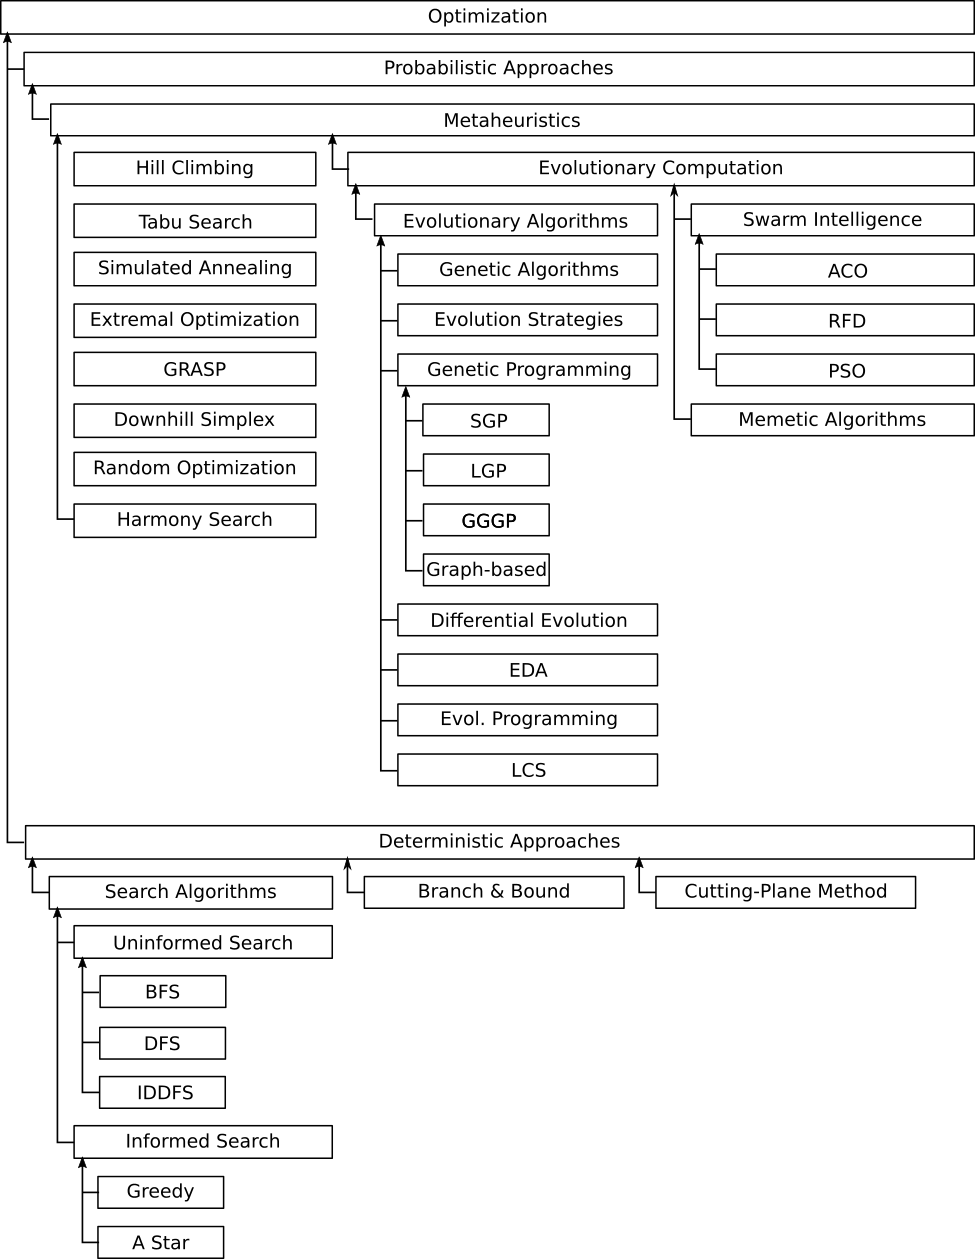
\includegraphics[width=.9\linewidth]{overview_optimisation_algorithm.png}
  \end{sidecaption}
\end{figure}

\subsection{Le domaine des algorithmes métaheuristiques, une sous-discipline de l'Optimisation}

\subsubsection{Q'est ce que l'optimisation ?}
\label{ssec:Optimisation}

Pour \textcite[22]{Weise2011}, l'optimisation \foreignquote{english}{ [...] is the process of solving an optimization problem, i. e., finding suitable solutions for it}, un problème d'optimisation nécessitant de trouver \foreignquote{english}{ [...] an input value $x^*$ for which a mathematical function $f$ takes on the smallest possible value (while usually obeying to some restrictions on the possible values of $x^*$ )}, la notation mathématique astérisque $^*$ désignant ici une valeur optimale.

Sortie de cette définition mathématique, l'optimisation peut également se définir par la mise en oeuvre d'algorithmes spécifiques. La littérature informatique met à disposition des programmeurs un ensemble d'algorithmes capables de fournir des solutions exactes dans un temps fini à un certain nombre de problèmes bien définis. C'est le cas par exemple des nombreux algorithmes de tri. Une autre classe d'algorithmes (\textit{optimization algorithms}) peut être employée lorsqu'il n'existe pas d'algorithme dédié (\textit{dedicated algorithms}), soit parce que le problème est trop spécifique, soit parce que personne n'a trouvé de solution efficace pour résoudre ce problème. 

Dans ce cadre, le terme d'optimisation globale \foreignquote{english}{ [...] is optimization with the goal of finding solutions $x^*$ for a given optimization problem which have the property that no other, better solutions exist.} Le terme \enquote{global} nécessite à la différence d'une recherche qui serait \enquote{locale}, de se concentrer sur l'obtention souvent plus couteuse et plus complexe d'un optimum global, minimum ou maximum, dominant par sa qualité l'ensemble des valeurs recherchées en entrée de la fonction à optimiser.

Bien que souvent beaucoup plus lent, moins précis, et plus consommateurs de ressources que les algorithmes dédiés, ces algorithmes d'optimisations nécessitent aussi beaucoup moins d'informations pour pouvoir être executés : \foreignquote{english}{Most often, these algorithms only need a definition of the structure of possible solutions and a function $f$ which tells measures the quality of a candidate solution. Based on this information, they try to find solutions for which $f$ takes on the best values.} \autocite[24]{Weise2011}

Ces algorithmes s'appuient donc sur différents types de stratégies pour tirer parti du peu d'information obtenue via cette fonction $f$. De nature très diverse, on retient pour séparer une première fois ces stratégies une typologie en deux classes. 

\begin{itemize}[label=\textbullet]
\litem{\textit{Probabilistic Approaches}} Les approches stochastiques désignées dans la fig. \ref{fig:S_OverviewOptimisation} sont capables de trouver un optimum assez rapidement, mais ne peuvent pas en garantir la propriété \enquote{globale}
\litem{\textit{Deterministic Approaches}} Les approches déterministes également désignées dans la fig. \ref{fig:S_OverviewOptimisation} peuvent certes garantir au moins théoriquement l'obtention d'un optimum global, mais s'éxecutent souvent au détriment d'un coût computationnel elevé.
\end{itemize}

Ces deux approches partagent également des difficultés communes, et découvrent leurs limites à des degrés divers en fonction des stratégies mise en oeuvre, dès lors que l'espace de recherche à parcourir devient trop important.

C'est le cas par exemple de l'espace de recherche de toute une sous-catégorie de problèmes \textit{NP-Complet} \Anote{np_complet_def} d'optimisation combinatoire \textit{Combinatorial Optimization Problems} (COP). Ce domaine contient par exemple les problèmes bien connus du voyageur de commerce \textit{Travelling salesman problem} (TSP), ou encore le problème du sac à dos \textit{Knapsack Problem} (KP) \Anote{note_knapsack}. Avec l'augmentation du nombre d'éléments entrant dans la définition de ces problèmes, il devient impossible de passer en revue l'ensemble des combinaisons (solutions possibles). Ce qui a pour conséquence de rendre difficile tout autant la découverte d'un optimum global, que la mesure de qualité de celui-ci, car pour établir cette dernière il nous faudrait logiquement connaitre la solution optimale, or c'est cela même que nous cherchons. 

Cette première typologie recoupe une autre propriété des algorithmes. La littérature informatique qualifie ainsi d'\textit{exacts} les algorithmes dont l'exécution garantit un résultat optimum à coup sûr, d'\textit{approximate algorithms} les algorithmes capables de donner une mesure proche d'un optimum sans pouvoir en garantir la qualité, et d'\textit{approximation algorithms} les algorithmes capables de donner une mesure proche d'un optimum assortie d'une preuve de qualité. Cette dernière classe n'est pas à confondre avec une classe d'algorithmes cherchant à conserver l'optimalité en limitant par diverses stratégies le coût temporel de résolution, mais bien l'inverse, relâcher la contrainte d'optimalité, mais aussi peu que possible. Les \textit{approximations algorithms} sont une donc une sous classe d'\textit{approximate algorithms}, et constituent une branche d'étude à eux seuls, car même dans le cas de problèmes \textit{NP-Complet}, ils offrent dans des dimensions raisonnables et propres à chacun des problèmes une solution sub-optimale d'erreur mesurable et donc potentiellement améliorable, voire comparable, notamment avec les résultats donnés de façon non analytique par d'autre stratégies.
%http://en.wikipedia.org/wiki/Approximation_algorithm#cite_ref-kann92onthe_3-4

On retrouve parfois rangé \enquote{en vrac} dans la classe des \textit{approximate algorithms} la classe des heuristiques et métaheuristiques, deux termes définis plus en détail dans la section suivante.

%On nomme métaheuristique (\textit{metaheuristic}) ce type d'algorithmes s'appuyant sur des heuristiques (\textit{heuristic}).

\subsubsection{Quelle définition peut on donner pour une heuristique (\textit{heuristic}) ? }
\label{ssec:heuristique}

Le terme heuristique \textit{heuristic} vient du Grec \textit{heuriskein} que l'on peut traduire par \foreignquote{english}{to find}, ou \foreignquote{english}{to discover}. D'usage plus large que dans la simple discipline informatique, nous retiendrons ici ce terme seulement sous son sens spécifique contextuel à l'optimisation. Rattaché à la définition d'un problème (\textit{problem dependent}), on définit une heuristique comme une mesure approximative pour définir la qualité d'une solution candidate \autocite[34]{Weise2011}.

%http://stackoverflow.com/questions/9140860/heuristic-function-for-finding-the-path-using-a-star
%http://stackoverflow.com/questions/9140860/heuristic-function-for-finding-the-path-using-a-star
%http://stackoverflow.com/questions/11779589/connection-between-a-star-search-and-integer-programming-extending-a-star
Si on se penche sur la classe d'algorithmes dédiés au problème de recherche du plus court chemin, les heuristiques sont souvent utilisées en appui des algorithmes de parcours de graphe, soit pour converger plus rapidement vers une solution optimale, soit pour justement se libérer de cette contrainte d'optimalité en visant un gain de temps au détriment de la précision. Si on prend par exemple l'algorithme de Djikstra, celui-ci n'utilise pas d'heuristique et garantit que le plus court chemin résultant sera optimal, car tous les chemins possibles entre le point de départ $A$ et le point final $B$ auront été analysés par celui-ci. Il est néanmoins connu comme étant très coûteux d'utilisation dès que le graphe dépasse un certain nombre de noeuds. L'algorithme déterministe $A^*$ s'appuie par contre sur une fonction heuristique $h(n)$ (une estimation du coût minimal reliant le noeud $n$ au noeud final) pour guider l'algorithme dans le processus incrémental de sélection d'un prochain noeud constitutif d'un chemin. En jouant sur cette heuristique, on est ainsi capable de déterminer si l'algorithme doit mettre la priorité sur la vitesse ou la précision, $h(0)$ étant équivalent ici à l'algorithme de Djikstra. Si l'heuristique est bien choisie (on dit ici que l'heuristique est admissible), alors $A^*$ garanti aussi l'optimalité du chemin trouvé, avec à la clef un coût computationnel moindre, car seule une partie des noeuds de l'ensemble du graphe auront été explorés par l'algorithme. Une autre heuristique misant plus sur la vitesse d'exécution pourra définir un chemin cette fois-ci sub-optimal avec un coût computationnel encore plus réduit. Il est à noter ici que l'utilisation d'une heuristique dans un programme n'est pas forcément motivée par la recherche d'un optimum global, mais par le gain de temps. Ainsi, un utilisateur peut très bien avoir les moyens d'obtenir un chemin optimal (Djikstra) sur une petite combinatoire de noeuds, mais peut vouloir prendre un raccourci en utilisant une méthode moins couteuse ($A^*$). Un scénario très souvent mis en avant dans la programmation de jeux sur ordinateur, où l'on cherche régulièrement à gagner du temps, tout en se rapprochant d'un comportement faillible imitant plus un adversaire de type humain.

La forme prise par une heuristique est variable, et peut aller comme vu ci-dessus avec l'exemple $A^*$ d'une simple fonction mathématique de coût intégrée à un algorithme classique de parcours de graphes, à un algorithme beaucoup plus complexe intégrant de multiples prises de décisions pour estimer ce même coût. Dans le livre \textit{Code Complete} de \textcite[12]{McConnell2004}, celui-ci donne un exemple assez parlant pour illustrer la subtile différence qui sépare la description d'un algorithme employé au sens courant pour désigner un algorithme déterministe exact fournissant à coup sûr une solution, et la description d'un algorithme déterministe ou stochastique heuristique (ou appuyé par une heuristique) fournissant seulement un guide pour trouver, éventuellement, une solution.

\foreignquote{english}{Here's an algorithm for driving to someone's house: Take Highway's 167 south to Puyallup. Take the South Hill Mall exit and drive 4.5 miles up the hill. Turn right at the light by the grocery store, and then take the first left. Turn into the driveaway of the large tan house on the left, at 714 North Cedar}

\foreignquote{english}{Here's an heuristic for getting to someone's house: Find the last letter we mailed you. Drive to the town in the return adress. When you get to town, ask someone where our house is. Everyone knows us - someone will be glad to help you. If you can't find anyone, call us from a public phone, and we'll come get you.}

Il faut toutefois éviter de considérer les heuristiques comme appartenant à la seule classe des \textit{approximate algorithms}, car le terme ne se laisse pas facilement enfermer dans une typologie trop simple. En effet de multiples problèmes trouvent une solution exacte jusqu'à un certain niveau de complexification, à partir duquel on fait généralement appel aux heuristiques, soit par un appel à d'autres méthodes intégrant des heuristiques, soit par une intégration d'heuristiques aux méthodes existantes. Ainsi de nombreuses classes d'heuristiques sont utilisées de façon transversale, et apparaissent donc aussi comme composantes manipulées dans la classes des \textit{approximation algorithms}. L'heuristique gloutonne \textit{greedy algorithm} \Anote{greedy_description} apparaît de façon transversale à la fois comme une solution d'approximation pour le \textit{Knapsack Problem} (KP) mais également comme moteur dans le cadre d'algorithmes déterministes exacts comme la recherche du plus court chemin de Djikstra. Un autre algorithme nommé \textit{A*} (\textit{A-Star}) qui englobe Djikstra comme cas particulier, est quant à lui capable de fournir tout à la fois une mesure exacte ou approximée en fonction de l'heuristique injectée et du niveau de complexité du problème abordé. 

\subsubsection{Quelle définition peut on donner pour une métaheuristique (\textit{metaheuristic}) ?}
\label{ssec:metaheuristique}

Le terme métaheuristique est d'origine plus moderne \autocite{Glover1986}, et a permis d'englober a posteriori des algorithmes jusque là qualifiés d'heuristiques. C'est le cas par exemple d'une bonne partie des algorithmes évolutionnaires, qui émergent principalement au cours des années 1960-1970. Cette remarque d'ordre historique est à l'origine d'une première ambiguité entre les termes auquelle il faut encore ajouter les inquiétudes exprimées par \textcite{Luke2013}. Pour ce dernier, le terme métaheuristique est en réalité plutôt malheureux pour définir cette catégorie d'algorithmes, car contrairement à ce que laisse entendre ce terme, \textit{une heuristique pour ou à propos d'une heuristique}, ce n'est pas de cela dont il s'agit ici.

Voici comment \textcite[8]{Brownlee2012} perçoit la différence entre les deux termes : \foreignquote{english}{Like heuristics, metaheuristics may be considered a general algorithmic framework that can be applied to different optimization problems with relative few modifications to adapt them to a specific problem. The difference is that metaheuristics are intended to extend the capabilities of heuristics by combining one or more heuristic methods (referred to as procedures) using a higher-level strategy (hence ‘meta’). A procedure in a metaheuristic is considered black-box in that little (if any) prior knowledge is known about it by the metaheuristic, and as such it may be replaced with a different procedure. Procedures may be as simple as the manipulation of a representation, or as complex as another complete metaheuristic. Some examples of metaheuristics include iterated local search, tabu search, the genetic algorithm, ant colony optimization, and simulated annealing.}

Le terme \enquote{méta-} renvoie plus en définitive au concept générique de \enquote{stratégie de recherche} prenant la forme d'un algorithme d'optimisation capable de mélanger, manipuler des heuristiques ou d'autres métaheuristiques (cf. points \ref{enum_meta_a} et \ref{enum_meta_h}) \Anote{def_meta_weise}. Contrairement aux heuristiques, les métaheuristiques se définissent plus comme un système fait de composants, dont la plasticité permet le support et l'interaction nécessaire au développement d'heuristiques plus ciblées (\textit{problem dependent}) \Anote{def_meta_sorensen}. La structure offre un patron d'usage initial (\textit{pattern}) qui reste indépendant du problème abordé (\textit{problem independent}) (cf. \ref{enum_meta_g}), tout en restant évolutif, comme le montre le fort développement de cette discipline depuis les années 1980. Ce principe de flexibilité, on le retrouve par exemple dans la classe des EC, comme le mettent bien en valeur Bach, Hammel et Schwefel en 1997, dans une publication introduisant l'EC dans la série renommée des \textit{IEEE Transactions} :

\foreignquote{english}{We argue that the most significant advantage of using evolutionary search lies in the gain of exibility and adaptability to the task at hand, in combination with robust performance (although this depends on the problem class) and global search characteristics. In fact, evolutionary computation should be understood as a general adaptable concept for problem solving, especially well suited for solving difficult optimization problems, rather than a collection of related and ready-to-use algorithms. The majority of current implementations of evolutionary algorithms descend from three strongly related but independently developed approaches: genetic algorithms,evolutionary programming , and evolution strategies. [...] The fundamental difference in the evolutionary computation approach is to adapt the method to the problem at hand. In our opinion, evolutionary algorithms should not be considered as off-the-peg, ready-to-use algorithms but rather as a general concept which can be tailored to most of the real-world applications that often are beyond solution by means of traditional methods. Once a successful EC-framework has been developed it can be incrementally adapted to the problem under consideration, to changes of the requirements of the project, to modifications of the model and to the change of hardware resources.} \autocite{Back1997a}

Enfin, toujours dans une tentative de positionner ce terme dans une typologie, il faut savoir qu'une classification trop rapide de ces méthodes dans les seuls \textit{approximate algorithms} peut également être critiqué. Si les méthodes métaheuristiques sont effectivement souvent connues pour ne pas avancer de preuve, des travaux récents montrent toutefois qu'il existe de nouveaux algorithmes permettant de garantir dans certaines conditions un optimum global (CP-Algorithm de \autocite{Reuillon2015}). Tout dépend donc du degré et de la nature que l'on veut bien associer à la notion d'\textit{approximation} lorsqu'il s'agit de fournir une mesure d'éloignement de l'optimum. Les \textit{approximation algorithms} semblent toutefois plus intéressés par l'établissement d'une preuve au sens mathématique, et se concentrent avant tout sur un ensemble relativement limité de problèmes d'optimisation discret, ce qui ne semble pas être le but des métaheuristiques dans les deux cas. \autocites[1-6]{Kann1992}[13-15]{Williamson2011} %Metaheuristics: From Design to Implementation Par El-Ghazali Talbi

%You could think of a heuristic like an approximate (not approximation) solution to a problem. The difference between approximate and approximation is that the first is about getting a good guess of the solution of a problem, but that you don't really know how good it is. The second is about getting a solution for which you can prove how close it is to the optimal solution.

Enfin bien d'autres sous classifications sont possibles prenant plus ou moins en compte les spécificités propres aux différents algorithmes, comme celle opposant par exemple les stratégies utilisées en interne pour parcourir l'espace de recherche (generationel contre \textit{steady-state}, ou individuel contre populationel), la dimensionnalité possible pour la résolution des problèmes (mono-objectif contre multi-objectif), l'inspiration d'origine (naturelle biologique contre inspirations autres), etc. 

Toute classification monocritère est donc rendue très difficile, une voie s'étant même ouverte pour tenter de classer ces algorithmes suivant la nature et le niveau d'opération de ces hybridations. L'origine de cette difficulté tient dans une pratique courante et assumée d'hybridation entre les différentes techniques afin de réunir le meilleur de chacune d'elles au sein de nouvelle proposition de recherche. De fait, il est important pour la suite de cerner au mieux la classe d'algorithme d'optimisation que nous allons aborder, et de définir pourquoi nous l'avons abordé. Nous nous intéresserons principalement dans la suite de cette présentation aux approches stochastiques métaheuristiques inspirées par la métaphore biologique, nommée \textit{Evolutionary Computation} (EC) ( voir figure \ref{fig:S_OverviewOptimisation}). La section \ref{xx} permettra de dégager les spécificités de cette subdivision, mais en attendant il nous faut d'abord présenter les principaux termes et concepts communs à cette classe d'algorithmes d'optimisation. 

Devant la difficulté d'établissement d'une définition englobante, plusieurs auteurs semblent s'accorder pour faire du rattachement d'un algorithme à cette catégorie, une correspondance plus ou moins lâche avec un ensemble de propriétés généralement observées. En évitant une définition trop vague ou trop restrictive, on espère ainsi récupérer dans cette classe certains hybrides intéressants. 

Voici un exemple de propriétés issues de \textcite{Blum2003} et traduites ci dessous :

%label=$\blacktriangleright$
\begin{enumerate}[label=(\alph*),labelindent=\parindent,leftmargin=*]
	\item Les métaheuristiques sont des stratégies qui \enquote{guident} le processus de recherche. \label{enum_meta_a}
	\item Leur objectif est d'explorer l'espace de recherche efficacement pour trouver les solutions quasi-optimales. \label{enum_meta_b}
	\item L'étendue des techniques que constitue la classe des algorithmes métaheuristiques va de la simple recherche locale à un processus d'apprentissage complexe. \label{enum_meta_c}
	\item Les algorithmes métaheuristiques sont approximatifs et la plupart du temps non déterministes. \label{enum_meta_d}
	\item Les métaheuristiques peuvent incorporer des mécanismes pour éviter d'être piégé dans une portion confinée de l'espace de recherche. \label{enum_meta_e}
	\item Les concepts de bases des métaheuristiques permettent d'adopter un certain degré d'abstraction dans la description. \label{enum_meta_f}
	\item Les métaheuristiques ne sont pas \textit{problem-specific}. \label{enum_meta_g}
	\item Les métaheuristiques peuvent faire usage d'une expertise du domaine au travers des heuristiques controlées par une stratégie de plus haut niveau. \label{enum_meta_h}
	\item La plupart des métaheuristiques actuelles font appel à une mémoire pour améliorer le processus qui guide la recherche. \label{enum_meta_i}
\end{enumerate}

Afin de mieux comprendre cette table de propriétés un peu abstraite, il est proposé de reprendre ces différents points au travers d'une lecture commentée, en commencant par une question ciblé sur la mécanique interne régissant ce type de technique.

\textit{Comment se matérialise la recherche de solutions optimisées dans une métaheuristique ?}

Si on considère les problèmes de combinatoires discrets comme \textit{TSP} ou \textit{Knapsack}, on a déjà vu que le nombre de combinaisons à évaluer lors d'une augmentation du nombre d'éléments participant à la définition du problème devient très vite problématique si on cherche à trouver une solution optimale exacte. Si on prend le cas d'un exemple plus ludique d'optimisations discrètes dans la branche des jeux (\textit{Combinatorial game theory}), le nombre de combinaisons légales possibles pour un plateau de 19 par 19 dans le jeu de GO chinois est estimé par \textcite{Tromp2007} à $2.08168199382×10^{170}$ . Même si certains auteurs comme Tromp estime qu'un tel calcul sera possible d'ici quelques années, les problématiques posés par ce jeu mettent au défi les meilleurs programmes en intelligence artificielle \autocite{Bouzi2001}, et cela malgré des progrès spectaculaires ces dernières années, via notamment l'utilisation d'heuristique plus efficace que les approches classiques \Anote{mcts_go}.  Dans le cas d'un problème continu discrétisé, comme la recherche des meilleures valeurs de paramètres pour une simulation, la mise en oeuvre d'un plan factoriel complet (d'autres types de stratégies beaucoup plus fines existent) pose un problème double. 

\hl{Correction orthographe à faire}
D'une part ce choix ne résout en rien la problématique combinatoire. Donnons un exemple plus concret, si une simulation possède 5 paramètres, chacun de ces paramètres étant discrétisé en 10 pas, cela nous donne déjà $10^5$ combinaisons possibles à évaluer. Si on considère que le modèle de simulation ainsi exécuté est stochastique (10 réplications), dans un délai relativement rapide (1 minute), la durée totale d'exécution de ce plan, pourtant relativement \enquote{grossier} d'un point de vue de la couverture de l'espace des paramètres, est environ égale à 2 années de calcul... La parallélisation d'un tel calcul, c'est à dire son execution sur plusieurs processeurs ou ordinateurs en parallèle, pourrait évidemment réduire ce temps de calcul à des dimensions plus raisonnables, mais c'est sans compter sur un deuxième problème, plus contraignant.

Avec le choix d'une telle maille pour la discrétisation des paramètres, c'est prendre le risque de passer à côté de solutions potentielles, une problématique contraignante d'autant plus qu'elle se complexifie avec l'augmentation du nombre de paramètres, comme le dicte le phénomène de \textit{Curse Dimensionality} établit par Richard Bellman. Ce problème est principalement d'ordre statistique, là ou 100 points peuvent suffire dans un espace entre $(0..1)$ de dimension $1$ pour commencer à inférer ($0.01$ de distance entre chaque point), 100 points dans un même espace $(0..1)$ de dimension $10$ ne couvre plus qu'une toute petite partie du volume disponible. Chaque point est alors entouré d'une large portion de vide qui rend délicates toutes inférences à partir d'une si faible couverture d'un tel espace. Pour obtenir une couverture équivalente avec une distance de $0.01$ entre chaque points, il faudrait disposer de $10^{20}$ points, ce qui semble considérable \autocite{Bellman1961}.

Contrairement à d'autres méthodes d'optimisations, les métaheuristiques font généralement appel à un processus d'échantillonnage (voir point \ref{enum_meta_b}) pour explorer de façon stochastique un espace de recherche de toute façon beaucoup trop vaste pour être parcouru de façon exhaustive. Cela permet de repousser en partie ce problème de couverture de l'espace de paramètres lié à l'augmentation de la dimensionnalité du problème, cas nous verrons que les méta-heuristique opérant dans des espace de paramètres discret mais aussi continu, sans qu'une discrétisation préalable soit nécessaire en amont.

C'est pour cela que \textcite[7]{Luke2013} nous propose de voir ce type de problème autrement, partant du postulat assez logique qu'une solution \enquote{même non optimale} est un point de départ pour l'amélioration de toute façon bien meilleure que \enquote{pas de solution du tout}.

\foreignquote{english}{ Metaheuristics are applied to \enquote{I know it when I see it} problems. They're algorithms used to find answers to problems when you have very little to help you: you don't know what the optimal solution looks like, you don't know how to go about finding it in a principled way, you have very little heuristic information to go on, and brute-force search is out of the question because the space is too large. But if you're given a candidate solution to your problem, you can test it and assess how good it is. That is, you know a good one when you see it.}  

\hl{schéma}

Suivant ce raisonnement, la connaissance d'un problème se construit au travers d'une confrontation répétée de nos représentations, de nos interrogations avec la forme réelle et encore inconnue prise par celui-ci. La carte de ce nouveau territoire se révélant peu à peu dans la projection sur l'espace des solutions des choix effectués lors de la sélection des nouveaux candidats à évaluer (solutions candidates).

Les métaheuristiques sont donc là pour faciliter l'exécution de cette tâche complexe et répétitive qui consisterait à améliorer notre connaissance du problème en proposant de façon pertinente de nouvelles solutions candidates à évaluer, ces dernières étant choisies si possible en fonction des résultats obtenus par les précédentes (voir point \ref{enum_meta_i}). La perspective d'une telle automatisation pose évidemment un certain nombre de questions. 

Quels sont les choix mis à disposition de l'optimiseur pour améliorer la réponse attendue des solutions candidates entre chaque incrément ? \autocite[19]{Weise2011} 

Une comparaison automatisée nécessite pour être mise en oeuvre de définir \begin{enumerate*}[label=(\alph*)]
\item sur quelle base se fonde l'évaluation d'une solution,
\item la comparaison entre les solutions évaluées, 
\item et la sélection de nouvelles solutions candidates.\end{enumerate*} Car l'optimiseur, tout comme nous, ne connait pas directement la forme prise par l'espace des solutions, et doit bien concevoir en interne les choix permettant, par la selection de nouvelles solutions candidates à évaluer, de progresser si possible vers une solution optimum.

De fait dans un tel scénario, et pour éviter une recherche aléatoire, l'évaluation de solution candidate renvoie à l'existence d'une expertise externe à l'optimiseur, le seul capable de formaliser ce qui différencie une bonne solution d'une mauvaise solution. On revient à parler ici d'heuristique, et de leurs diversités, car si celles-ci interviennent dans l'évaluation des solutions candidates (a), elles interviennent aussi dans les autres cas (b) et (c). Elles se présentent sous la forme de différents types de connaissances, interrogent différents espaces, et s'intègrent souvent sous la forme de composants dans la structure plastique des métaheuristiques.

L'injection de connaissance (voir point \ref{enum_meta_h} )dans ce type d'algorithme métaheuristique est donc double, et opère à la fois de façon précise dans la formalisation d'un ou de plusieurs critères qui vont servir pour l'algorithme optimiseur à déterminer la qualité, bonne ou mauvaise, d'une solution candidate; et de l'autre elle intervient cette fois ci de façon moins contrôlable dans la façon dont l'expérimentateur va construire et paramétrer une métaheuristique pour l'adapter au mieux à son problème. La qualité interne (paramètre, structure) de la métaheuristique définit aussi en quelque sorte le processus d'exploration, ce qui explique aussi la dépendance de ce type d'algorithmes à l'environnement qu'ils doivent explorer.

\begin{figure}[ht]
	\begin{sidecaption}[fortoc]{Projection du vecteur de points $\{a \dotsc n\}$ dans l'espace des objectifs. Les couleurs représentent les différents axes de projection ordonnés de 1 à 3 sur $(x,v)$ et de 1 à 4 sur $(y,v)$}[fig:spacePspaceOmultimodal]
	 \centering
	 	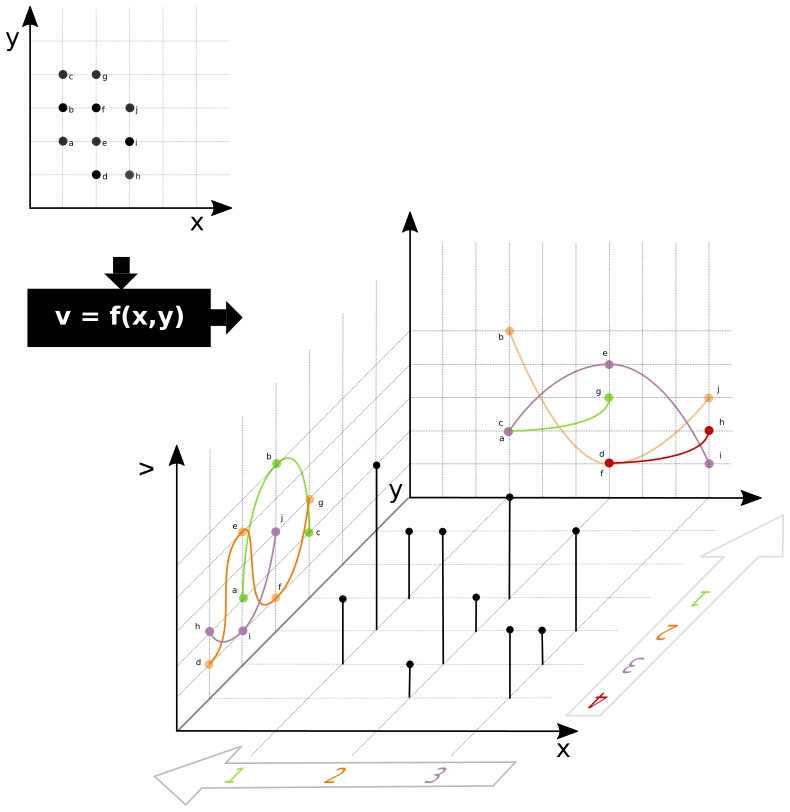
\includegraphics[width=.9\linewidth]{espaceP_espaceO_multimodal.pdf}
	\end{sidecaption}
\end{figure}

L'objectif est rendu complexe car la relation entretenue entre ces deux espaces, celui des solutions candidates disponibles, et celui des évaluations est bien souvent dissymétrique. Pour mieux comprendre cette relation, la figure \ref{fig:spacePspaceOmultimodal} illustre cette correspondance des solutions candidates $\{a \dotsc n\}$ décrites par leurs coordonnées $(x,y)$ lorsqu'elles sont projetées dans l'espace des objectifs $\mathbb{Y}$ en suivant la transformation attendue par la fonction boite noire de dynamique non linéaire $f(x,y)$. Les valeurs $v = f(x,y)$ des différentes solutions candidates sont également projetées sur le plan 2D $(x,v)$ et $(y,v)$ pour mieux visualiser la forme prise par cette surface en 2D.

\begin{figure}[!htbp]
	\begin{sidecaption}[fortoc]{Les couleurs indiquent la  des valeurs $v = f(x,y)$ mesurée dans la figure \ref{fig:spacePspaceOmultimodal}, sachant qu'on cherche à minimiser la valeur de v :
\parbox{\marginparwidth}{
\begin{enumerate}[label={},labelindent=0pt,leftmargin=*]
        \item \sqbox{tangoBlue1} indique une fitness minimale, cf. qui maximise $v$
        \item \sqbox{tangoOrange1} indique une fitness intermédiaire et,
        \item \sqbox{tangoRed1} indique une fitness maximale, cf. qui minimise $v$
\end{enumerate}}}[fig:xyspacePspaceOmultimodal]
	 \centering
	  \subbottom[]{
	 	
\includegraphics[width=0.4\linewidth]{xyespaceSolutionCandidate_a.pdf}
	 	\label{subfig_xyespaceSolutionCandidate_a}}
	 \subbottom[]{
	 	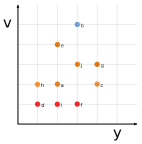
\includegraphics[width=.4\linewidth]{xyespaceSolutionCandidate_b.pdf}
	 	\label{subfig_xyespaceSolutionCandidate_b}}
	 \subbottom[]{
		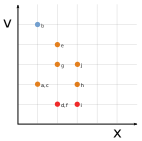
\includegraphics[width=.4\linewidth]{xyespaceSolutionCandidate_c.pdf}
		\label{subfig_xyespaceSolutionCandidate_c}}
	\end{sidecaption}
\end{figure}

Pour visualiser la valeur $v$ prise par chacune des solutions candidates, on projette celle-ci dans l'espace $(x,y)$, ce qui nous permet de mieux constater l'éclatement des valeurs de $v$ sur la figure \ref{fig:xyspacePspaceOmultimodal}.

Deux solutions proches dans l'espace des solutions candidates peuvent amener à des résultats très différents, et inversement, pour deux évaluations proches peuvent correspondre des solutions candidates très éloignées, comme le détaille la figure \ref{fig:xytrajectoire}. Il s'agit d'une propriété bien connue des fonctions non linéaires, qu'elles soient décrites de façon explicite via le formalisme mathématique, ou de façon implicite dans l'expression des dynamiques complexes de modèles de simulation.

Il est clair que l'information récoltée par un tel déplacement basé sur une distance euclidienne dans le plan $(x,y)$ n'est pas vraiment pourvoyeur d'intuitions sur l'emplacement possible des meilleures solutions (voir figure \ref{fig:xytrajectoire}). Il semble par exemple plus intéressant pour l'optimiseur d'accéder aux solutions par le prisme d'ensembles construits sur la base d'une valeur $v$ commune (voir figure \ref{fig:xyspacePspaceOmultimodal}). Une information qui peut être exploitée de multiples façons, toujours en permettant à l'optimiseur de déterminer un nouvel ensemble de solutions candidates à évaluer.

\begin{figure}[!htbp]
	\begin{sidecaption}[fortoc]{Représentation de deux déplacements dans l'espace des solutions candidates et son équivalent dans l'espace des objectifs
	\parbox{\marginparwidth}{
	\begin{enumerate}[label=(\alph*),labelindent=\parindent,leftmargin=*]
	        \item Partant de $b$, on se déplace d'une unité vers $c$ ou $a$, ce qui dans l'espace des objectifs équivaut également à un déplacement vers $h$; $v=2$ pour $v_h, v_a, v_c$
	        \item Partant de $b$, on se déplace toujours d'une unité vers $f$, ce qui dans l'espace des objectifs équivaut également à un déplacement vers $d$ et $i$; $v=1$ pour $v_d,v_i,v_f$
	\end{enumerate}}}[fig:xytrajectoire]
	 \centering
	  \subbottom[]{
	 	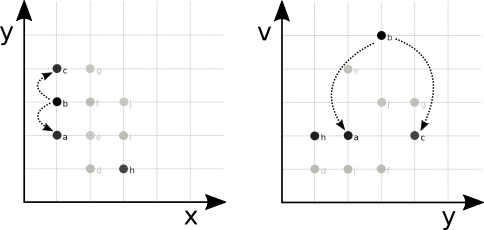
\includegraphics[width=0.6\linewidth]{xytrajectoire_a.pdf}
	 	\label{subfig_xytrajectoire_a}}\qquad
	 \subbottom[]{
	 	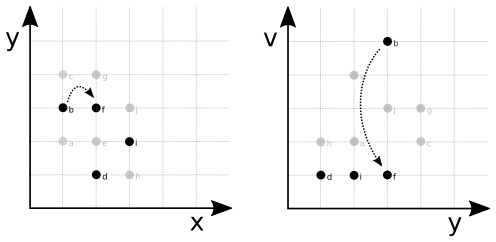
\includegraphics[width=.6\linewidth]{xytrajectoire_b.pdf}
	 	\label{subfig_xytrajectoire_b}}
	\end{sidecaption}
\end{figure}

Si l'obtention d'une cartographie complète d'un tel espace de solutions peut être l'objectif de ce type de raisonnement, la recherche d'un optimum en est un autre. Dans un cas on aura tendance à maximiser la diversité dans le choix de solutions candidates à évaluer, afin d'essayer de couvrir au mieux le territoire à explorer. Cette idée on la retrouve dans l'établissement d'une \textit{fitness landscape}, ou dans sa version multi-objectif, d'un \textit{problem landscape} \autocite[93-94]{Weise2011}, un paysage cumulé de l'espace des objectifs indiquant toutes les valeurs prises par ceux-ci au cours de l'exploration \Anote{paysage_cumule}. Un espace mis à profit par l'optimiseur pour améliorer la proposition de solution candidate, par exemple en se basant sur la construction de cluster de valeurs intéressantes comme indiqué précédemment, ou encore en cherchant à favoriser les zones de cet espace encore peu explorées, etc. Alors que dans le cas d'une optimisation pour la calibration ou la prédiction, trouver le plus rapidement possible un minimum local ou global peut constituer un objectif suffisant.

En réalité, ces deux objectifs sont souvent liés, et c'est souvent l'expertise humaine intervenant de façon externe à l'optimiseur qui va déterminer l'importance de l'un ou de l'autre dans la stratégie à suivre. Dans le cas par exemple d'une optimisation de paramètres nécessaire à la marche efficiente d'une centrale nucléaire, la découverte d'un minimum local robuste peut s'avérer beaucoup plus intéressante qu'un minimum global instable. La topologie proche de l'espace des solutions déjà exploré peut constituer un facteur de connaissance d'intervention plus ou moins importante dans l'expertise d'une bonne ou d'une mauvaise solution. 

Cette mécanique on la retrouve également à un autre niveau, dans le fonctionnement interne des métaheuristiques. En effet, celles-ci s'appuient le plus souvent sur la métaphore biologique évolutive pour mettre en tension une recherche de solutions guidée toute à la fois par l'\textit{exploration} (trouver des solutions originales), et l'\textit{exploitation} (améliorer les solutions existantes). 

\begin{figure}[!htbp]
\begin{sidecaption}[fortoc]{Recherche d'un minimum global.}[fig:hmap2ab]
 \centering
 \subbottom[Une fonction $f(x)$ présentant un unique minimum global]{
 	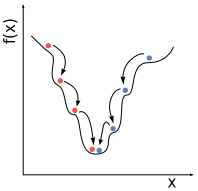
\includegraphics[width=.4\linewidth]{heightmap2a.pdf}
 	\label{subfig_hmap2ab_a}}\qquad
 \subbottom[Une fonction $f(x)$ présentant un minimum local et global]{
	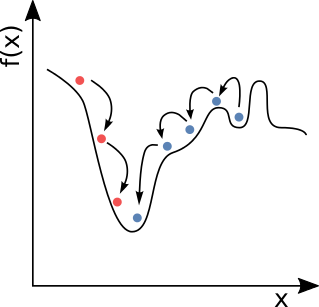
\includegraphics[width=.4\linewidth]{heightmap2b.pdf}
	\label{subfig_hmap2ab_b}}
\end{sidecaption}
\end{figure}

Les opérateurs intervenant comme stratégies dans la médiation de ces deux concepts sont conçus pour éviter à l'optimiseur un certain nombre d'écueils. Trop longue pour être abordée ici de façon exhaustive, cette liste évoquant les problèmes et solutions qui résultent du rapport entre les formes de problèmes abordés et les faiblesses génériques ou dépendantes des métaheuristiques utilisées, \textcite{Weise2011} en donne une description experte sur une centaine de pages. On peut également se référer à une autre synthèse, abordant ces problèmes avec un angle un peu plus spécifique aux algorithmes évolutionnaires, réalisée en 2001 par \textcite[316-445]{Deb2001}.

En se limitant aux pièges dépendant de la topologie de l'espace des solutions (voir point \ref{enum_meta_e}), \textcite[140]{Weise2011} a proposé un tableau synthétique dont on extrait ici quelques exemples légèrement modifiés pour éclairer notre argumentaire. Les exemples des figures \ref{fig:hmap2ab} et \ref{fig:hmap2cd} mettent en oeuvre un optimiseur générant de façon incrémentale de nouvelles solutions, chacune représentée par un point. Il faut donc lire ces exemples en tenant compte du fait qu'ils présentent une représentation cumulative des différents points parcourus dans le temps par l'optimiseur.

La figure \ref{fig:hmap2ab} démontre un fonctionnement normal de l'optimiseur, capable quelque soit son placement initial (rouge ou bleu), de trouver le minimum global d'une fonction relativement simple \ref{subfig_hmap2ab_a}. Un comportement équivalent est observable dans la figure \ref{subfig_hmap2ab_b}, le compromis \enquote{exploitation - exploration} étant suffisant pour que l'optimiseur bleu surmonte l'obstacle posé par la présence d'un minimum local dans cette fonction.

\begin{figure}[!htbp]
  \begin{sidecaption}[fortoc]{Deux types de fonctions sont rendues difficiles à optimiser du fait d'une topologie marquée.}[fig:hmap2cd]
  \centering
  \subbottom[Une fonction $f(x)$ multimodale acceptant plusieurs minimum locaux, et un seul minimum global]{
  	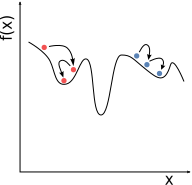
\includegraphics[width=.4\linewidth]{heightmap2e.pdf}
  	\label{subfig_hmap2cd_c}}\qquad
  \subbottom[Une fonction $f(x)$ contenant très peu d'information de gradient pour guider l'optimiseur]{
	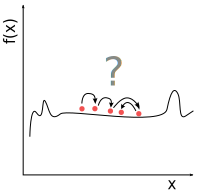
\includegraphics[width=.4\linewidth]{heightmap2c.pdf}
  	\label{subfig_hmap2cd_d}}
 \end{sidecaption}
\end{figure}

A l'inverse, on perçoit bien sur ce schéma \ref{subfig_hmap2cd_c} quel effet peut avoir un déséquilibre entre les deux stratégies, une exploitation trop appuyée au détriment de l'exploration amenant souvent à une convergence \Anote{def_convergence} prématurée, c'est-à-dire à un piège dans un optimum local. 

La figure \ref{subfig_hmap2cd_d} montre également que face à une topologie de fonction présentant un plateau relativement uniforme, l'optimiseur sera en peine pour trouver un minimum, même local. Un paramétrage différent de l'exploration pourra peut être résoudre ce problème, sans pour autant que l'on en soit sur. 

Ce qui nous permet d'évoquer une faiblesse connue des métaheuristiques, héritée des remarques déjà faites sur les algorithmes d'optimisations stochastique \Anote{stochastic_note} dans laquelle on les place habituellement. La découverte garantie d'une solution globale optimale est en général difficile avec ce type d'algorithmes (voir point \ref{enum_meta_d}) \Anote{equipe_mixite}, au moins pour deux raisons : 

\begin{enumerate}
\item la variabilité qui opère lors de la selection des solutions candidates à un instant $t$ ne permet pas de garantir qu'il n'existe pas quelque part une solution candidate sélectionnée à $t+1$ dont l'évaluation révélera un meilleur optimum. La définition d'un critère d'arrêt est donc rendue délicate.
\item La variabilité dans l'établissement d'une trajectoire de recherche implique qu'un algorithme de même qualité puisse passer une première fois à coté d'un optimum, et une deuxième fois trouver celui-ci. 
\end{enumerate}

\begin{figure}[!htbp]
\begin{sidecaption}[fortoc]{Représentation d'une navigation indirecte de l'optimiseur dans un espace de solution $z = f(x,y)$.}[fig:hmap1]
  \centering
  \subbottom[]{
  	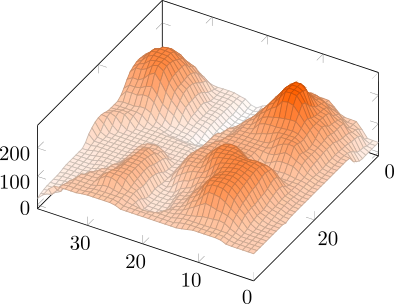
\includegraphics[width=.4\linewidth]{heightmap1a.png}
  	\label{subfig_hmap_a}}\qquad
  \subbottom[]{
	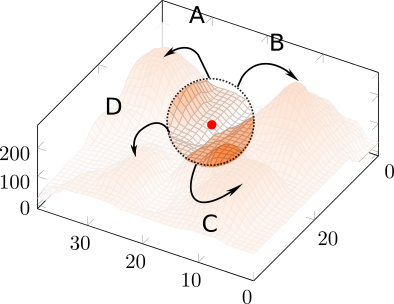
\includegraphics[width=.4\linewidth]{heightmap1b.png}
  	\label{subfig_hmap_b}}
\end{sidecaption}
\end{figure}

Pour mieux comprendre les problèmes posés par des espaces de solutions multi-modaux, déjà figurés en deux dimensions dans \ref{subfig_hmap2cd_c}, on représente cette fois ci dans la figure \ref{fig:hmap1} l'optimiseur dans un espace en trois dimensions similaire à celui vu dans la figure \ref{fig:spacePspaceOmultimodal}, à la recherche d'un optimum global. La fonction ainsi représentée comporte deux entrées $(x,y)$, et une sortie $z = f(x,y)$ représentant la valeur numérique résultat de l'optimisation.

Attention à la lecture de ces schémas, il ne faut pas oublier que l'optimiseur \textbf{ne se déplace pas directement} sur le terrain visible dans la figure \ref{subfig_hmap_a}, et pour laquelle celui-ci n'a justement aucune visibilité. C'est un peu comme visualiser un labyrinthe de l'extérieur sur une feuille, puis de l'intérieur quand on s'y projette, la difficulté pour résoudre celui-ci n'est plus la même. La visibilité dont dispose l'optimiseur est celle des résultats de solutions candidates déjà évaluées (voir point \ref{enum_meta_i}). Il s'agit donc de proposer de nouvelles solutions candidates soit en les composant à partir d'une manipulation des solutions candidates déjà évaluées, soit en introduisant de toutes nouvelles solutions candidates prises de façon aléatoire. Au cours de l'itération mesurant la progression de l'algorithme, c'est bien l'évaluation de cette nouvelle population de solutions candidates qui détermine si il y'a effectivement eu un déplacement qualitatif dans l'espace des solutions evaluées. Le déplacement du point rouge dans cet espace n'est donc effectif que si on trouve à un instant $t + 1$ une solution plus intéressante qu'à l'instant $t$.

A partir des résultats de la première solution candidate évaluée figurée ici en rouge dans \ref{fig:hmap1}, les opérateurs de recherches soumis à l'aléa d'une recomposition ou d'un tirage aléatoire peuvent tout à fait proposer un candidat à $(x,y)_{t+1}$ qui débouche sur un résultat $z = f(x,y)$ plaçant l'optimiseur dans le sillon d'un gradient de pente parmi plusieurs. Ce qui mènera probablement l'optimiseur à découvrir des optimums de qualités très différentes : $A$ (local), $B$ (global), $C$ (local), $D$ (local). 

Autrement dit, en plus de la stochasticité inhérente de ces algorithmes, non seulement un algorithme de type $A$ n'aura pas les mêmes résultats qu'un algorithme de type $B$, mais celui-ci sera également différent d'un algorithme $A'$ du fait d'un paramétrage différent.

Comme déjà évoqué dans les différentes définitions, on retrouve ici la qualité de flexibilité des métaheuristiques, permettant de transformer ce qui pourrait de prime abord paraitre pour un défaut, en qualité. L'utilisation de celle-ci permettant d'étendre toujours un peu plus leurs champs d'utilisation, en facilitant la réponse aux questions suivantes \Anote{q_ppr} : 
\begin{enumerate}
\item  \foreignquote{english}{What parameter settings do I use to get good results when applying heuristic method X to problem Y?}
\item  \foreignquote{english}{How do I adjust the parameters of heuristic X so I get better results on problem Y?}
\item \foreignquote{english}{Which is \enquote{better}, heuristic X or heuristic Y?}
\end{enumerate}

On pourrait ainsi ne retenir que cette citation de source inconnue, lorsqu'elle définit une métaheuristique comme \foreignquote{english}{ a pretty good rule for finding pretty good rules.}

Cette flexibilité vient compléter et compenser efficacement cet horizon de connaissance assez limité, nécessaire à une généricité d'emploi. Les métaheuristiques fournissent ainsi le support générique initial pour en faire un outil d'usage indépendant du problème, tout en fournissant les outils pour favoriser également leur propre modification en vue d'une amélioration de résultat pour un problème donné. Elle cumule donc en quelques sortes les deux propriétés de dépendance et d'indépendance face à un problème donné. 

De plus, la recherche dans cette discipline ne se contente pas d'organiser une forme de compétition qui mènerait à elle seule, par l'apprentissage répété de fonctions aussi standardisées que celles utilisées dans les figures précédentes, à une surestimation de certains algorithmes \Anote{test_fonction_surutilisation}, et se nourrit également d'une recherche plus appliquée à des problématiques réelles. Ce qui permet par effet retour, d'espérer voir appliquer à des formes de problèmes génériques, des opérateurs dédiés à l'origine à des problématiques spécifiques. La construction et l'évaluation d'heuristique plus performante servant toujours indirectement une cause plus générale.

Enfin, une des propriétés qui n'a pas encore été introduite dans ce résumé est la capacité de notation et de description abstraite des métaheuristiques (voir point \ref{enum_meta_f} ). Des concepts de plus haut niveau sont introduits pour désigner l'expression et la manipulation d'heuristiques et de classes d'heuristiques dans un système composant la métaheuristique. Mais avant de pouvoir introduire ces subtilités de typologie propre à chaque classe de métaheuristique, il faut également rappeler l'existence d'une base commune de formalisation mathématique permettant la description des problèmes. Autrement dit, cela revient à introduire ou à poser sur une partie des mots déjà utilisés dans cette section, un certain nombre de notations mathématiques d'utilisation relativement standard dans cette communauté informatique utilisant les métaheuristiques.

Il nous restera également à aborder dans la section suivante, la question des \textbf{moyens} mis à disposition de l'optimiseur pour opérer la selection de nouveaux candidats à évaluer. Jusqu'ici seule une représentation de ces solutions candidates dans l'espace des solutions candidates possibles a été abordée, ainsi que l'espace contenant les résultats des solutions candidates évaluées. Mais ces deux espaces ne constituent pas les véritables espaces sur lesquels l'optimiseur est amené à travailler, et cela bien qu'il puisse les intégrer à son expertise pour la selection de nouveaux candidats à l'évaluation \Anote{remarque_section_metaheuristique}. 

\hl{les 4 paragraphe ci dessous sont à faire descendre avec notation mathématique, pour compléter la section suivante, et sans briser le suspens ?}

L'introduction d'un nouvel \enquote{espace de recherche} est nécessaire, et  correspond à la somme des entrées, des paramètres, sur lequel l'optimiseur va pouvoir jouer directement, afin de modifier cette fois-ci indirectement l'expression de la solution candidate ensuite évaluée.

Autrement dit, il faut retenir qu'une solution candidate fait partie d'un espace de solutions candidates possibles, et que l'exploration de ce dernier est dépendant des bornes fixées par l'expert pour délimiter l'espace de recherche de chacun des entrant, notamment pour limiter le champ de recherche de l'optimiseur à celui des valeurs empiriquement et théoriquement possibles. Ce qui introduit aussi la possibilité d'une nouveau \textit{mapping} entre les valeurs de ces deux espaces, de recherche, et du phénomène à évaluer, qui ne sont pas nécessairement de même nature. 

On peut s'appuyer sur l'exemple de bras robotisé donné par \autocite{Weise2011} pour illustrer ce cas. On a d'un côté les paramètres de positionnement des éléments de bras d'un robot, contraint par la structure théorique de celui-ci, et de l'autre l'expression spatiale finale du bras représentatif de cette combinaison de paramètres dans l'espace des solutions possibles, potentiellement infini, et dont on n'a pas la maitrise directe. L'optimiseur s'appuie ensuite sur l'évaluation de cette configuration spatiale à l'aide des critères qu'on lui a donné pour induire des opérations non pas dans l'espace d'expression spatialisé du bras, mais dans l'espace de recherche des vecteurs de paramètres permettant l'amélioration de ce résultat.

\subsubsection{Une formulation mathématique standardisée pour encadrer les problèmes d'optimisations et les métaheuristiques}
\label{ssec:math_opti}

%search space p 82
%structure p 101
% pareto ranking p 275
																								
Pour comprendre comment se déroule de façon générale la résolution d'un problème d'optimisation, il faut poser un certain nombre de notions qui nous seront utiles par la suite. Cet exercice de description plus mathématique et générique s'appuie là encore principalement sur les écrits de \textcite{Weise2011}

La première étape selon Weise dans la construction d'un problème d'optimisation est de définir le type de structure qui peut être associée à l'expression des solutions possibles et spécifiques à notre problème.

Autrement dit, il s'agit de déterminer quel est l'espace dans lequel évolue la donnée figurant la solution attendue pour cette optimisation. L'expression de cette solution peut appartenir à l'espace des réels $\mathbb{R}$, comme par exemple une valeur numérique se rapportant à l'optimisation d'une fonction mathématique. Mais celle-ci peut également s'exprimer dans un repère beaucoup plus complexe, en faisant référence par exemple à un repère géométrique définissant le cadre  d'une forme à optimiser comme une pièce de moteur, une pièce d'avion, etc. \autocite[43]{Weise2011}

Cet espace du problème (\textit{problem space}) $\mathbb{X}$ est défini comme \foreignquote{english}{ [...] the set containing all elements $x$ which could be its solution.} 

Une solution candidate $x$ est quant à elle définie comme \foreignquote{english}{ [...] an element of the problem space $ \mathbb{X}$ of a certain optimization problem.}

L'objectif de l'optimisation est donc de trouver par le biais d'un algorithme adapté l'ensemble des solutions candidates $x^*$ appartenant à l'espace du problème répondant le mieux aux critères définis par l'utilisateur. Ce qui suppose de pouvoir qualifier une solution candidate $x_1$ tiré de $\mathbb{X}$ par rapport à une autre solution candidate $x_2$ elle aussi tiré de $\mathbb{X}$.

\textit{Une deuxième étape logique serait donc d'établir comment se fait la mesure établissant la qualité d'une solution ?}

Comme défini précédemment, ce qui va guider l'algorithme optimiseur dans sa prise de décision, c'est l'évaluation d'une fonction heuristique, ou d'une fonction objectif (\textit{objective function}) \Anote{difference_objective_heuristique} 

\foreignquote{english}{An objective function $f: \mathbb{X} \mapsto \mathbb{R}$ is a mathematical function which is subject to optimization.}

Cette fonction objectif lorsqu'elle prend pour paramètre un élément candidat $x$ pris dans l'espace du problème $ \mathbb{X}$ renvoie une valeur définissant sa qualité par rapport au problème posé. \autocite[44]{Weise2011}

\sloppy La plupart des problèmes nécessitent toutefois d'optimiser plusieurs critères simultanément. La relation entre ces critères peut d'ailleurs être elle aussi multiple : dépendante (conflictuelle, en harmonie), indépendante. Nous allons donc nous intéresser directement à la définition de ce type de problème, résumable ainsi :  $min(f_1(x), \dotsc, f_k(x)$ avec $k > 2$

La littérature fait également plus souvent référence à ce type de problème en faisant appel à une notation sous forme de fonction vecteurs. Un ensemble $\vec{f} : \mathbb{X} \mapsto \mathbb{R}^n$ fait de $n$ fonction objectif $f_i : \mathbb{X} \mapsto \mathbb{R}$ avec $\forall i \in 1 \dotsc n$. Appliqué à une solution candidate $x \in \mathbb{X}$ cette fonction renvoie un vecteur de réel de dimension $n$ qui peuvent être projeté dans un espace $\mathbb{R}^n$, aussi appelé espace des objectifs (\textit{objective space}) $\mathbb{Y}$.

En résumé, à chaque association d'un vecteur de fonction objectif $\vec{f}$ et d'une solution candidate $x$ correspond après évaluation un vecteur de réel de dimension $n$ permettant le positionnement de la solution candidate dans l'espace $\mathbb{R}^n$ des objectifs aussi nommé $\mathbb{Y}$.

C'est à partir du positionnement des solutions candidates dans cet espace $\mathbb{Y}$ que l'optimiseur va décider de la prochaine solution candidate à évaluer. 

\textit{Dès lors, comment ce choix se fait-il dans une perspective multi-objectifs a priori contradictoires ?}

\begin{figure}[!hbtp]
	\begin{sidecaption}[fortoc]{ Pour la valeur $x = 0$, $f1(x) = 0 $ et $f2(x) = 4 $, pour $x = 2$,  $f1(x) = 4 $ et $f2(x) = 0 $ , donc la configuration inverse. La solution pour minimiser les deux fonctions $f1$ et $f2$ tient donc forcément dans un compromis dans la valeur prise par $x$.}[fig:S_Schaffer]
	\centering
	\begin{tikzpicture}[line cap=round,line join=round,>=triangle 45,x=1.0cm,y=1.0cm]
	\draw [color=cqcqcq,dash pattern=on 1pt off 1pt, xstep=1.0cm,ystep=1.0cm] (-5,-1) grid (5,5);
	\draw[->,color=black] (-5,0) -- (5,0);
	\foreach \x in {-5,-4,-3,-2,-1,1,2,3,4}
	\draw[shift={(\x,0)},color=black] (0pt,2pt) -- (0pt,-2pt) node[below] {\footnotesize $\x$};
	\draw[->,color=black] (0,-1) -- (0,5);
	\foreach \y in {-1,1,2,3,4}
	\draw[shift={(0,\y)},color=black] (2pt,0pt) -- (-2pt,0pt) node[left] {\footnotesize $\y$};
	\draw[color=black] (0pt,-10pt) node[right] {\footnotesize $0$};
	\clip(-5,-1) rectangle (5,5);
	\draw[color=ttttff] plot[raw gnuplot, id=func2] function{set samples 100; set xrange [-4.9:4.9]; plot x**2};
	\draw[color=fftttt] plot[raw gnuplot, id=func3] function{set samples 100; set xrange [-4.9:4.9]; plot (x-2)**2};
	\begin{scriptsize}
	\draw[color=ttttff] (-2.26,6.14) node {$f$};
	\draw[color=fftttt] (-0.24,6.14) node {$g$};
	\end{scriptsize}
	\end{tikzpicture}
 \end{sidecaption}
\end{figure}

\sloppy Si on prend pour exemple la fonction multi-objectifs de Schaeffer décrite dans l'équation \ref{eq:schaffer}, $f1(x)$ and $f2(x)$ deux fonctions objectifs à minimiser $\vec{f} = (f1(x),f2(x))^T$  avec $\vec{f}: \mathbb{X} \mapsto \mathbb{R}^2$

\begin{equation} \label{eq:schaffer}
Minimize = 
	\begin{cases}
	 f1(x) = x^2 \\
	 f2(x) = (x-2)^2
	\end{cases}
\end{equation}

Si on superpose les deux fonctions comme dans la figure \ref{fig:S_Schaffer}, on voit bien qu'elles sont contradictoires, il s'agit donc de trouver un compromis. 

Cette opération que nous pratiquons tous les jours sans forcément le savoir peut être plus facilement expliquée en faisant appel à cet exemple concret. Dans le cas d'un acheteur à la recherche d'une voiture à la fois économe de par sa faible consommation et si possible disponible à un moindre coût, celui-ci devra bien se plier à l'exercice de positionnement des voitures résumé dans le graphique \ref{fig:voiture}. 

Dans le graphique \ref{subfig_voiture:b} on constate rapidement que le modèle de voiture que l'acheteur va acheter à de fortes chances de se trouver dans la liste de voitures $\{ A,B,C,D,E \}$ colorées en rouge, aussi appelée front de Pareto, ou optimum de Pareto. Ce terme apparait en économie en 1950, en référence directe des travaux de l'économiste italien Vilfredo Pareto. Le lecteur plus curieux de ces questions pourra trouver de multiples points d'entrées sur ces questions dans les publications suivantes \autocites{Ehrgott2012,Koksalan2011,Koksalan2013}. 

\begin{figure}[!htbp]
	\begin{sidecaption}[fortoc]{Exemple simplifié d'une catégorisation de voitures selon deux axes comprenant d'une part le coût d'achat et d'autre part la consommation de chaque voiture.}[fig:voiture]
	\centering
	  \subtop[]{
  	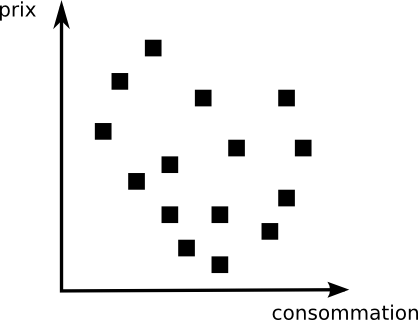
\includegraphics[width=.3\linewidth]{opti1.png}
  	\label{subfig_voiture:a}}\qquad
    \subtop[]{
	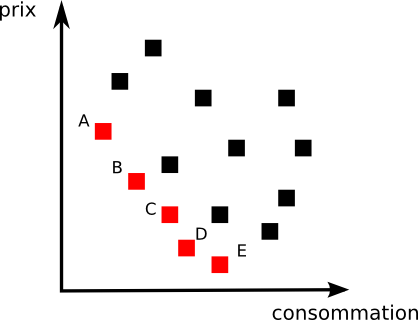
\includegraphics[width=.3\linewidth]{opti2.png}
  	\label{subfig_voiture:b}}
    \subtop[]{
  	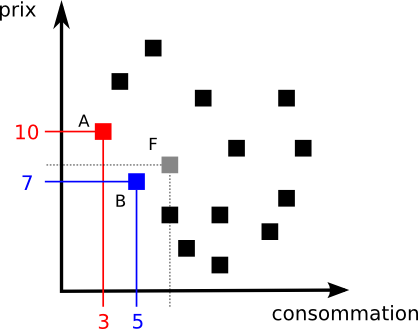
\includegraphics[width=.3\linewidth]{opti3.png}
  	\label{subfig_voiture:c}}
 \end{sidecaption}
\end{figure}

\sloppy En regardant en détail les capacités des voitures figurant dans ce front \ref{subfig_voiture:c}, on voit bien que chacune d'entre elle domine une partie des autres voitures sur au moins un des deux objectifs. Si on prend le cas de la voiture F, celle-ci n'est pas prise en compte dans les solutions optimums, car le point est dominé sur ses deux objectifs par d'autres voitures : $ prix(B) < prix(F) < prix(A) $ et $consommation(A) < consommation (B) < consommation(F)$.

Le front de Pareto renvoie un ensemble de solutions compromis optimal, l'expertise finale sur la ou les solutions à adopter est donc le résultat d'un choix expert externe introduit comme support à l'algorithme optimiseur. Dans notre exemple, l'acheteur devra pour finaliser son achat mettre en avant au moins un des deux critères afin de départager les voitures.

Si certains algorithmes ont introduit cette expertise par le biais d'une sélection interactive guidant l'optimiseur à chaque étape de sa recherche, ce n'est pas cette usage qui nous intéresse ici. L'expertise n'intervient qu'une fois les solutions convergées, dans l'observation des résultats finaux.

Dans notre cas, on considère que l'optimiseur doit sélectionner avec les moyens qu'on lui a fournis les solutions candidates sur lesquels il doit miser pour converger. Il doit donc être capable de séparer les solutions en appliquant un ou plusieurs critères de séparation. Il existe plusieurs types de stratégies (\textit{Agreggation based, Criterion based, Dominance based, Indicator based}), et chacune d'elles peut être croisée ou dérivée en de multiples variantes \autocites[28]{Zitzler1999a, Deb2001}[7]{Liefooghe2009}. Nous limiterons ici notre analyse à un seul de ces cas, en nous focalisant d'ores et déjà sur les méthodes les plus utilisées en EC, basées sur la dominance celles-ci sont directement inspirées des travaux de Pareto.

% TODO : Finir ce paragraphe historique rapide, qui permettra de faire la différence ensuite avec les algorithmes inspirés par Pareto.
% TODO : Ajouter ref de Goldberg sur les sciences humaines + GA dans le chapitre 1

\begin{figure}[!htbp]
	\begin{sidecaption}[fortoc]{Graphique en deux dimensions des fonctions objectifs $f_1$ et $f_2$ du tableau \ref{tab:pranking}}[fig:pranking_a]
		\centering  	
		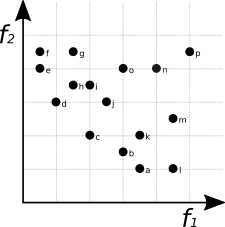
\includegraphics[width=.4\linewidth]{pareto_ranking_a.pdf}
	 \end{sidecaption}
\end{figure}

\begin{table}[!htbp]
\begin{sidecaption}[fortoc]{Tableau de résultats des fonction objectifs $f_1$ et $f_2$ pour un vecteur de solutions candidates $\{a \dotsc p\}$ dans l'espace des objectifs $\mathbb{Y}$, et résultat du \textit{Pareto Ranking}}
	[tab:pranking]
	\centering
	\begin{tabular}{>{$}l<{$}>{$}l<{$} >{$}l<{$} >{$}l<{$}}
			\toprule
			\text{solutions candidates} & f_1 & f_2 & \text{dominé par} \\
			\midrule
			a      & 3.5    & 1    &  \varnothing \\
			b      & 3      & 1,5  &  \varnothing \\
			c      & 2      & 2    &  \varnothing \\
			d      & 1      & 3    &  \varnothing \\
			e      & 0.5    & 4    &  \varnothing \\
			f      & 0.5    & 4.5  &  \{e \}  \\
			g      & 1.5    & 4.5  &  \{d,e,f,h \} \\
			h      & 1.5    & 3.5  &  \{d \} \\
			i      & 2      & 3.5  &  \{c,d,h \} \\
			j      & 2.5    & 3    &  \{c,d \} \\
			k      & 3.5    & 2    &  \{a,b,c \} \\
			l      & 4.5    & 1    &  \{a \} \\
			m      & 4.5    & 2.5  &  \{a,b,c,k,l \} \\
			n      & 4      & 4    &  \{a,b,c,d,e,h,i,j,k,o \} \\
			o      & 3      & 4    &  \{b,c,d,e,h,i,j \} \\
			p      & 5     & 4.5   &  \{a,b,c,d,e,f,g,h,i,j,k,l,m,n,o \} \\
			\bottomrule
	\end{tabular}
  \end{sidecaption}
\end{table}

Pour comprendre comment cette stratégie et définir mathématiquement la notion d'optimum de Pareto, il faut introduire la notion de \textit{dominance} sur lequel elle s'appuie. Pour cette tâche on s'appuie sur les définitions données par \textcite[65]{Weise2011} :

\foreignquote{english}{An element $x_1$ dominates (is preferred to) an element $x_2 (x_1 \dashv x_2)$ if $x_1$ is better than $x_2$ in at least one objective function and not worse with respect to all other objectives.} 

Ce qui dans le cas d'une minimisation se traduit mathématiquement par les conditions suivantes : 

\begin{align*}
	(x_1 \dashv x_2) \Leftrightarrow &\forall i \in 1 \dotsc n \Rightarrow - i f_i (x_1) \leq i f_i (x_2) \land \\
	&\exists j \in 1 \dotsc n : j f_j (x_1) < - j f_j (x_2)
\end{align*}

Cette notion de \textit{domination} ($\succ$) \Anote{notation_dominance} permet de dégager ces trois possibilités

\begin{itemize}
\item $x_1$ domine $x_2$ , qui peut également s'écrire $x_1 \succ x_2$
\item $x_1$ est dominé par $x_2$
\item $x_1$ n'est pas comparable avec $x_2$
\end{itemize}

Celle-ci possède les propriétés suivantes, qui définissent dans l'espace des objectifs $\mathbb{Y}$ un \textit{strict partial order} : 

\begin{enumerate}
\item{\textbf{non reflexive}}  $x_1$ ne peux pas se dominer lui même
\item{\textbf{non symétrique}} $ x_1 \succ x_2$ n'implique pas $x_2 \succ x_1$, alors que l'opposé est vrai, $x_1 \succ x_2$ implique $x_2$ ne domine pas $x_1$
\item{\textbf{transitive} }
\end{enumerate}

Différents degrés de dominance ont été développés, comme par exemple la notion de \textit{strong dominance} : $x_1$ domine fortement $x_2$ ($x_1 \succ \succ x_2$) si $x_1$ est strictement meilleur que $x_2$ sur tout ses objectifs. 

Pour bien comprendre comment se construit l'ensemble $X^*$ de solutions non dominées $x^* \in \mathbb{X}$ ,on peut étudier en détail comment la dominance se calcule entre les points $e$ et $f$ présentés sur la figure \ref{fig:pranking_a}.

\begin{table}[!h]
	\centering
	\begin{sidecaption}[fortoc]{Application des règles de dominance aux points $e$ et $f$. \\ \\
		   \begin{tabular}{>{$}l<{$}>{$}l<{$} >{$}l<{$}}
					\toprule
					 & f1 & f2 \\
					\midrule
					e      & 0.5    &  4   \\
					f      & 0.5    & 5,5  \\
					\bottomrule
			\end{tabular}\\ \\ 
			(a) $e \succ f$ car e est bien le meilleur sur au moins un des deux objectifs, et n'est pas pire sur aucuns des autres objectifs ($e \succeq f$ ) \\ 
			(b) f ne domine pas e car f n'est pas meilleur sur aucun des deux objectifs et il est pire sur au moins un des deux objectif}[tab:pranking]
		
		\begin{minipage}{0.5\textwidth}
			\centering
			\subbottom[e est dominé par f ?]{
				\begin{tabular}{>{$}l<{$}>{$}l<{$} >{$}l<{$}}
					\toprule
					    & f1 & f2 \\
					\midrule
					e \leq f & \text{true} & \text{true} \\
					e < f   & \text{false}  & \text{true} \\
					\bottomrule
				\end{tabular}
		 	\label{pranking_a}}
		 \end{minipage}\hspace{1em}
		 \begin{minipage}{0.5\textwidth}
		 	\centering
			\subbottom[f est dominé par e ?]{
				\begin{tabular}{>{$}l<{$}>{$}l<{$} >{$}l<{$}}
					\toprule
					  & f1 & f2 \\
					\midrule
					f \leq  e & \text{true} & \text{false} \\
					f < e  & \text{false}  & \text{false} \\
					\bottomrule
				\end{tabular}
			\label{pranking_b}}
		\end{minipage}
  \end{sidecaption}
\end{table}

Les solutions admises parmi le front de Pareto (voir figure \ref{fig:frontoptimal}) sont donc ici toutes celles qui ne sont pas dominées faiblement ($\succeq$), ce qui revient à exclure les points $f$ et $l$ du front optimum $\{a,b,c,d,e\}$ car ils sont dominés faiblement ($e \succeq f$); alors que dans le cadre d'une dominance forte ($\succ \succ$), ceux-ci auraient fait partie du front $\{a,b,c,d,e,f,l\}$. En effet si on prend toujours le cas de $e$ et $f$, la condition testant que $e$ est strictement meilleur que $f$ sur tous les objectifs n'est pas remplie. %Cet ensemble de cardinalité forcément inférieure ou égale est qualifié \enquote{d'ensemble fort non dominé} (\textit{Strongly non dominated set}).

\begin{figure}[!htb]
	\begin{sidecaption}[fortoc]{Tracé du front optimum à partir du calcul des individus non dominés, cf. l'ensemble vide $\varnothing$ dans le tableau \ref{tab:pranking}}[fig:frontoptimal]
		\centering
		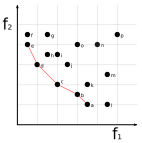
\includegraphics[width=.4\linewidth]{pareto_front.pdf}{
		}
  \end{sidecaption}
\end{figure}

Le front de Pareto n'est en général jamais entièrement couvert, cela pour diverses raisons : 

\begin{itemize}
\item L'évaluation de la fonction à optimiser est souvent coûteuse, comme dans le cas de modèle de simulation dont l'exécution peut prendre jusqu'à plusieurs dizaines de minutes, 
\item La zone d'exploration est volontairement bornée du fait des objectifs des expérimentateurs, 
\item La stochasticité oblige l'exécution de nombreuses réplications d'une même évaluation,
\item On dispose de ressources finies, or l'espace du front est souvent continu et non borné en dehors des contraintes que l'on aura nous-mêmes fixées.
\end{itemize}

Selon \textcite[70]{Weise2011} et \autocite[19]{Zitzler1999a}, on peut s'aider dans cette tâche d'établissement d'un front de Pareto correct en étant attentif aux points suivants:

\begin{enumerate}
\item{\textbf{Proximité}} Les solutions découvertes doivent être les plus proches possibles du front de Pareto optimal.
\item{\textbf{Diversité}} Si le front optimal possible est trop large, la répartition des solutions \textit{spread} doit être maximisé sur toute la surface de celui-ci, si possible suivant une distribution uniforme.
\item{\textbf{Pertinence}} Les solutions découvertes doivent correspondre aux intérêts définis par le problème, et n'ont aucun intérêt si l'opérateur humain ne peut, ou ne sait les utiliser.
\end{enumerate}

On retrouve dans ces objectifs la tension entre exploration et exploitation, le front de Pareto devant être exploité de façon homogène, tout en garantissant à terme (et si possible le plus vite possible) la convergence vers une zone d'intérêt pour l'expérimentateur (voir figure \ref{fig:convergence_diversite}). Les métaheuristiques n'ayant pas d'apriori sur la forme de problème abordée, c'est dans l'originalité, la diversité des constructions proposées qu'une solution optimale et dédiée peut être trouvée. Il est donc très difficile de faire un listing des meilleures stratégies, et des meilleures combinaisons de stratégies permettant une sélection garantie des meilleurs candidats en fonction de ces objectifs, l'établissement de cette liste ne pouvant être que contextuelle d'un problème d'optimisation donné. 

\hl{ref no free lunch theorem }? Wikipedia : Le théorème du « no free lunch » explique qu’aucune instance de métaheuristique ne peut prétendre être la meilleure sur tous les problèmes. Une métaheuristique (M) n’est performante que pour une classe de problème (P) donnée.

Heureusement, un certain nombre de combinaisons, souvent éprouvées par de multiple tests sur des fonctions aux caractéristiques et difficultés soigneusement étudiées (ZDT, etc.), se démarquent par des capacités de résolution acceptable. C'est d'ailleurs souvent sur cette première base que se construisent ensuite les améliorations nécessaires à une réponse optimale, cela en partie grâce à la flexibilité des composantes caractéristique des métaheuristiques. 

\begin{figure}[!htbp]
  \begin{sidecaption}[fortoc]{Convergence et maintien de la diversité au sein du front de Pareto}[fig:convergence_diversite]
  \centering
  \subbottom[Un front de pareto sans maintien suffisant de la diversité]{
  	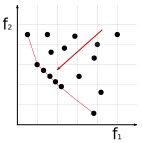
\includegraphics[width=.4\linewidth]{pareto_convergence_a.pdf}
  	\label{subfig_convergence_diversite:a}}\qquad
  \subbottom[Un front de pareto avec maintien de la diversité]{
	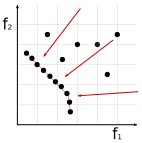
\includegraphics[width=.4\linewidth]{pareto_convergence_b.pdf}
  	\label{subfig_convergence_diversite:b}}
 \end{sidecaption}
\end{figure}

\textit{Une fois défini cet ordre partiel entre les solutions candidates évaluées, sur quelle base l'optimiseur prend sa décision pour sélectionner les individus les plus prometteurs ? et comment celui-ci garantit l'évolution des solutions candidates selectionnées au regard des trois objectifs fixés ?}

Comme le dit de façon très claire,\textcite[94]{Weise2011} \foreignquote{english}{Such comparisons, however, only state whether one candidate solution is better than another one or not, but give no information on \textbf{how much} it is better or worse and \textbf{how interesting} it is for further investigation. Often, such a scalar, relative measure is needed.}

L'optimiseur n'ayant pas les capacités pour comparer des fonctions entre elles, c'est par l'attribution d'un scalaire caractérisant chaque vecteur $z^* \in \mathbb{Y}$ résultat de l'évaluation d'une solution candidate, que celles-ci vont pouvoir être départagées. On parle de \enquote{fonction d'utilité}, ou de \enquote{fonction \textit{fitness}} pour désigner cette opération de transformation dont le résultat $z$ est utile uniquement en se plaçant dans le référentiel de l'optimiseur. Il s'agit d'un classement relatif des solutions les unes par rapport aux autres, calculés indépendamment des valeurs prises par les fonctions objectives, et intégrant un certain nombre d'autres critères, définis en réponse aux exigences des trois objectifs déjà évoqués (respect de la diversité, qualité de convergence, pertinence vis-à-vis du problème). 

Ainsi, un des tout premiers paramètres à intégrer dans le calcul de cette fonction \textit{fitness} tient évidemment dans le choix d'une stratégie pour tirer un meilleur parti des informations récoltées dans l'application de cet ordre partiel sur l'espace $\mathbb{Y}$. Là ou des algorithmes vont appuyer la sélection des solutions à partir d'un calcul de rang (je ne garde que les $n$ premiers rangs), d'autres vont le faire à partir d'un décompte des non dominés (je ne garde que les individus non dominés $< n$), à partir d'une profondeur (je ne garde que les $n$ premiers fronts), ou encore en mélangeant ces trois informations (voir le résultat du calcul de ces trois informations dans \ref{tab:pranking} \hl{a finir}) A cela il faut également ajouter la diversité de choix à disposition dans la selection d'une dominance, par le changement de l'opérateur utilisé dans le calcul (\textit{weak dominance}, \textit{strong dominance}, etc.), ou même la relaxe de celui-ci (\textit{epsilon-dominance}). Des choix de première importance, car ils interviennent directement dans la construction de l'ensemble de solution retenue.

C'est donc dans l'espace des objectifs $\mathbb{Y}$ que se révèle la première information pertinente pour l'optimiseur, nous indiquant, peu importe la forme de l'une ou de l'autre des fonctions et le positionnement des points sur celles-ci, une première sélection de solutions parmi les solutions candidates évaluées sur laquelle l'effort de l'optimiseur doit porter en priorité.

Mais lorsque l'on reprojette les résultats du front de Pareto dans l'espace figurant la dynamique supposée de chacune des deux fonctions objectifs, on observe que la prise de décision basée sur le seul ordonnancement des solutions n'est pas suffisante pour garantir une selection optimale des meilleurs candidats à l'évolution (voir figure \ref{fig:mo_landscape}). 

La forme des fonctions dans cette figure est représentée en pointillé car elle n'est qu'une description temporaire d'un paysage en partie inconnu, en attente d'être révisée par l'évaluation de nouveaux points. Le tracé d'un paysage ne se confond plus comme cela pouvait être le cas dans une optimisation mono-objectif avec la valeur prise par la fonction objectif, et doit maintenant intégrer un intermédiaire supplémentaire plus complexe qui est le calcul d'une fonction \textit{fitness}, et dont la formulation, dépendante de nombreuses stratégies, va modifier les solutions choisies dans le futur, et donc modifier la façon dont on va découvrir l'approximation de ce paysage, cela de façon indépendante aux objectifs choisis. \autocite{Weise2011}

\begin{figure}[!htbp]
	\begin{sidecaption}[fortoc]{Projection du front de Pareto optimal (point \sqbox{tangoBlack1}), et des autres solutions candidates dominées (point \sqbox{tangoGrey1}) sur l'espace de variation du paramètre $x \in \mathbb{R}$, un schéma inspiré par \textcite[67]{Weise2011}
	\parbox{\marginparwidth}{
	\begin{enumerate}[label={},labelindent=0pt,leftmargin=*]
	      \item \sqbox{tangoBlue1} $f_{1}(x)$
	      \item \sqbox{tangoRed1} $f_{2}(x)$
	\end{enumerate}}\\
	Les fonctions $f_{1}(x)$ et $f_{2}(x)$ sont représentées en pointillé car elles sont inconnues de l'optimiseur, et ne servent que de repère au lecteur pour mieux comprendre comment un paysage caractérisant l'intersection des deux fonctions peut émerger durant l'optimisation, et pourquoi cela peut être intéressant d'intégrer son analyse à l'optimiseur.}[fig:mo_landscape]
	 \centering
	 	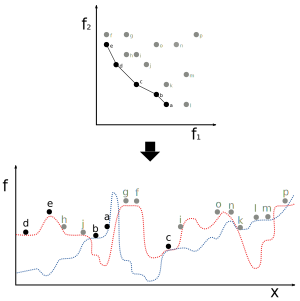
\includegraphics[width=0.8\linewidth]{multi_objective_landscape.pdf}
	\end{sidecaption}
\end{figure}

%on se rend également compte qu'un surplus d'information tiré de l'exploitation d'autres espaces pourrait être utile au choix de l'optimiseur

%\Anote{weise_multi2D}
Déjà beaucoup plus difficile à imaginer que dans l'exemple précédent de l'équation de Schaeffer, la re-projection des solutions candidates évaluées se fait sur un nouvel espace $\mathbb{G}$ (voir figure \ref{fig:relation_espaces}), qui inclu l'ensemble de tout les éléments $g \in \mathbb{G}$ qui peuvent être manipulés par les opérateurs de recherche à disposition de l'optimiseur \autocite[82]{Weise2011}. Un processus détaillé un peu plus tard dans cette section.

Dans notre cas $x \in \mathbb{R}$, on a donc un paramètre qui est manipulable et peut prendre une infinité de valeurs dans le cadre des contraintes définies pour $x$ (par exemple une valeur de 0 à 10 pour $x$) \Anote{remarque_resolution}. L'espace $\mathbb{G}$ contient la codification du problème, ce qui par exemple dans le cadre de simulation, se traduit pour chaque élément $g$ par l'attribution d'un vecteur de paramètres définissant les entrées de la simulation sur lequel l'optimiseur va pouvoir \enquote{jouer} pour optimiser les différentes fonctions objectifs.

La fonction $gpm : \mathbb{G} \mapsto \mathbb{X}$ est une translation opérée lorsque les deux espaces sont de nature différente, par exemple pour passer d'un espace Binaire à un espace de Réels $\mathbb{B} \mapsto \mathbb{R}$. Dans le cadre de simulations, les deux espaces sont souvent de nature similaire $\mathbb{G} = \mathbb{R}$. On pourra se référer à \textcite[86-88]{Weise2011} pour plus de détails.

\begin{figure}[!htbp]
	\begin{sidecaption}[fortoc]{Résumé des relations entre les différents espaces dans une optimisation}[fig:relation_espaces]
		\centering
		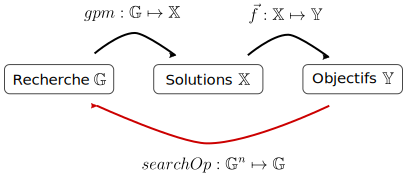
\includegraphics[width=.7\linewidth]{objectifsToSearchSpace.pdf}
  \end{sidecaption}
\end{figure}

%D'une part, l'observation de dynamiques en partie contraires sur ces deux fonctions $f_1$ et $f_2$ nous permet de constater encore une fois pourquoi un déplacement de l'optimiseur sur l'une ou l'autre des fonctions dirigé par la recherche d'un optimum n'a aucun sens. 

L'opération de sélection des solutions candidates est souvent rattachée au processus de convergence. L'objectif de l'optimiseur est d'évaluer au mieux le potentiel de chacune des solutions durant cette phase de sélection pour intégrer et conserver les meilleurs éléments à son référentiel entre deux itérations. On imagine pourtant très bien bien l'effet que peut avoir une sélection trop restrictive sur le maintien de la diversité. C'est le cas par exemple si l'optimiseur ne décide de garder que le front de Pareto, on voit bien sur la figure \ref{fig:mo_landscape} à quel point la couverture de la dynamique des deux fonctions ressortirait considérablement appauvrie à la suite d'un tel choix. On en déduit que la frontière entre stratégies de convergence, et stratégie de maintien de la diversité doit être assez perméable pour garantir le choix de solutions candidates pertinentes en dehors du seul front de Pareto. Zitler \hl{ref autre que ppt à trouver} retient par exemple parmi ces classes de stratégies celle s'appuyant sur le couple associant espace des objectifs et au choix la dominance, la densité, le temps, ou encore la chance. Ce sont des heuristiques qui vont intervenir en amont sur la qualité et la diversité des solutions candidates (par exemple les stratégies de \textit{sharing}, \textit{crowding}, etc.) qui peuvent ensuite être manipulées par les opérateurs de recherches de l'optimiseur.

Viennent ensuite les stratégies de recombinaison des solutions selectionnées, créatrices de nouvelles solutions candidates à évaluer. Un processus qui peut être là aussi rattaché tout autant au maintien de la diversité qu'à une volonté de convergence accrue. Il n'y a là encore aucune règle d'applications spécifique, et tout dépend de l'objectif fixé de façon initiale ou au cours de l'expérimentation. Ainsi, certaines stratégies intégrés aux opérateurs peuvent être mis en place pour limiter une convergence trop rapide des solutions (\textit{premature convergence}) liée à une perte de diversité, alors que d'autres vont tenter d'accélérer cette convergence par la mise en oeuvre d'opérateur de recherche plus agressif, soit pour trouver le plus rapidement possible un minimum (ou maximum) local, soit car la topologie de l'espace des objectifs est de topologie difficile. 

La sélection de candidats à la manipulation dans l'espace des objectifs $\mathbb{X}$ se réfère, une fois projetée dans cet espace $\mathbb{G}$, aux éléments $g$ accessibles à la manipulation par les opérateurs de recherche de la fonction $searchOp$. Chacun de ces opérateurs, dont le nombre et la nature est un paramètre de l'optimiseur, s'appuie sur la transformation d'une ou plusieurs solutions candidates dirigée par la création d'un nouvel élément $g$, dont on attend si possible un meilleur résultat à l'itération suivante. Un postulat très fort est posé par ce type de méthodes d'optimisation, l'introduction de petites variations sur les valeurs de l'espace de recherche est également censée apporter de petites variations dans l'espace des objectifs, que cela résulte en une amélioration ou en une dégradation de la qualité. Appelée \textit{strong causality} \Anote{note_strong}, cette propriété est évidemment dépendante de la forme prise par le paysage du problème (\textit{problem landscape}), et plus celui-ci est accidenté, rugueux, plus sa résolution est considérée comme complexe \Anote{note_weak}.

En relation avec cette observation, l'éclatement de cette population de solutions candidates évaluées sur le paysage nous permet de constater (voir la figure \ref{fig:mo_landscape}) à quel point la notion de distance entre les points parait différente entre ces deux espaces. $f$ et $c$ apparaissent ici beaucoup plus proches de trouver un optimum global que $a$ et $b$, pourtant plus proche de $c$ dans l'espace des objectifs. On voit bien ici que la sélection de solutions candidates intéressantes peut intégrer d'autres informations utiles, en supplément de celle fournit par l'analyse de $\mathbb{Y}$, au travers de l'analyse de cet espace $\mathbb{G}$; et cela toujours afin de guider au mieux l'optimiseur dans la selection des candidats à l'évolution. Un croisement du positionnement des individus $f$ et $c$ donnerait ainsi une bien meilleure valeur de $x$ à évaluer, probablement meilleure que celle d'un individu $a$ et $c$. Si la solution $f$ avait été éliminée sur le fait d'une sélection aux critères plus drastiques, c'est aussi la possibilité d'un croisement fructueux avec $c$ qui disparait.

%A ces stratégies principales s'ajoute un autre ensembles de stratégies, dont certaines sont plus spécifiques, ou constitutives des types d'algorithmes utilisés. %Le maintien d'une diversité de solutions entre les itérations fait partie de ces stratégies qui font partie d'un set plus large de stratégies permettant de contrer l'émergence des différentes difficultés (stochasticité, topologie, etc.) caractéristique d'un problème de résolution unique. 

%Généralement nommé \foreignquote{english}{Pareto Ranking} \Anote{utilisation_pareto_ranking} aussi nommé par Weise \foreignquote{english}{Prevalence Ranking}.

% Ou introduire la notion d'individu ?

\begin{figure}[!ht]
	\begin{sidecaption}[fortoc]{Résumé simplifié du déroulement d'une optimisation selon \textcite[109]{Weise2011}}[fig:resume_opti]
		\centering
		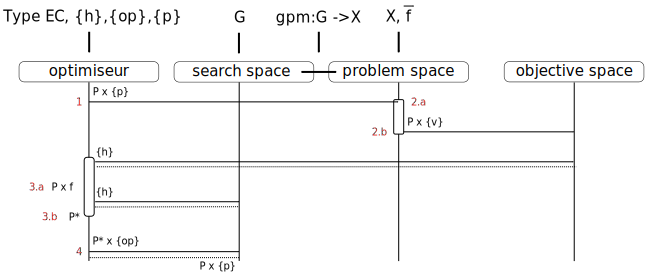
\includegraphics[width=\linewidth]{espace_resume.pdf}{
		}
  \end{sidecaption}
\end{figure}

La description des étapes de la figure résumé \ref{fig:resume_opti} sont les suivantes :

\begin{itemize}[label=\textbullet]
	\litem{1} Une première population $P \in {1 \dotsc n}$ de vecteurs paramètres ${p}$ est générée par l'optimiseur ou introduite par l'expérimentateur, puis soumis à évaluation.
	\litem{2.a} La fonction à optimiser est évaluée autant de fois qu'il y a de vecteurs ${p}$ 
	\litem{2.b} Les fonctions objectifs $\vec{f}$ sont calculés, ce qui permet de créer autant de vecteur ${v}$ correspond au résultats des fonctions qu'il y a de $P$ évalué. Ces vecteurs $P(v)$ peuvent être positionné dans un espace des objectif $\mathbb{Y}$ 
	\litem{3.a} Le calcul de fitness $f$ est effectué pour chaque élément de $P$ en utilisant les informations rapportés par un ensemble d'heuristiques sur $\mathbb{Y}$ et, ou $\mathbb{G}$
	\litem{3.b} A partir du calcul de cette fitness $f$ pour chacun des éléments de $P$, on selectionne les $P^*$ meilleurs éléments.
	\litem{4} A partir d'un ensemble d'opérateur ${op}$ on va générer de nouveaux vecteurs de paramètres $P(p)$, qui va constituer le nouveau jeu de solution candidates à évaluer à l'étape (1), et dont on espère qu'elles seront si possible meilleures que les précédentes.
\end{itemize}

\hl{Manque la notion d'invididu = fitness + genotype + phenotype}

% Injection de connaissance se fait un peu partout pour la construction d'une fitness.

% Penser à dire qu'il y a plusieurs stratégies de comparaison autre que Pareto ? 

%Première fois utilisé en 1989

%Si on transfère ce langage neutre au vocabulaire que l'on peut trouver courrament dans l'EC, alors l'espace des solution devient le \textit{phenome}, et le point de cet espace qui correspond à la solution candidate devient un \textit{phenotype}.

%\begin{figure}
%\begin{sidecaption}[fortoc]{ POM cycle for developping theory for an agent behavior \autocite[245]{Railsback2012}}[fig:S_syntheseGrim]
%  \centering
% 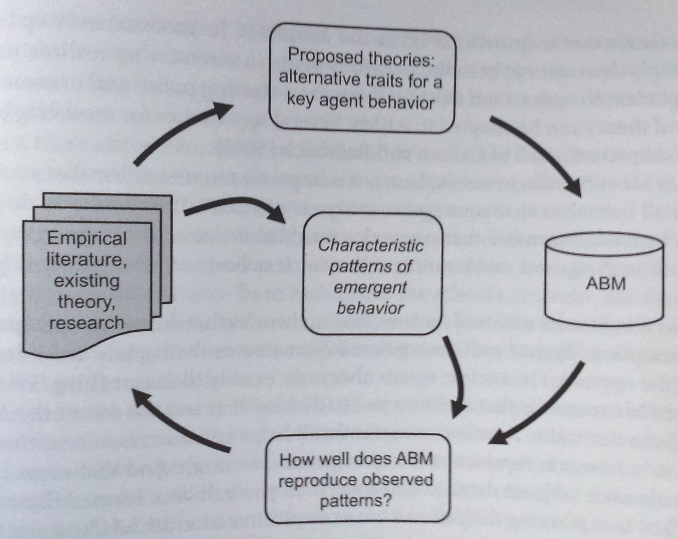
\includegraphics[width=.9\linewidth]{cyclePOMcomportement.png}
%  \end{sidecaption}
%\end{figure}


%Dans notre étude, l'objet à optimiser ne se réfère pas à une expression mathématique, mais à un modèle de simulation, sur lequel on va déterminer un ensemble de critères qui vont faire figure d'équivalent de ces fonction objectives. Dans ce cas d'utilisation, l'optimisation est plus souvent employé comme une forme de calibration inversé \autocite{Grimm2011}, dans laquelle on cherche à déterminer si il existe un ou plusieurs jeu de valeur de paramètres du modèles de simulation respectant la plage de valeur viable empiriquement qui permettent de maximiser l'obtention d'un ou de plusieurs critères experts. Il est plus parlant dans notre cas de désigner l'espace de recherche comme l'espace des paramètres.  

La branche des métaheuristiques EC que nous allons étudier plus spécifiquement s'appuie sur l'observation de phénomènes naturels, comme l'évolution, ou l'organisation, pour la construction et la mise en oeuvre d'algorithmes mimant certaines propriétés intéressantes de ces processus, cela sans être rattaché à une contrainte de réalisme biologique.

\subsection{Les métaheuristiques bio-inspirées, la branche des Algorithmes Evolutionnaires}

\subsubsection{Un rapide historique de la discipline}

On a déjà rapidement décrit dans la section à propos de l'Artificial Life \ref{p:heritage_complexe} les deux voies qu'il était possible d'emprunter dans l'intéret porté sur la définition du processus naturel d'évolution. 

Il existe en effet au moins deux façons aujourd'hui d'introduire des développements informatiques se rapportant à ce processus évolutif. D'un côté, les tentatives de reproduction plus ou moins fidèles des différents mécanismes à l'oeuvre dans le processus d'évolution mettent en avant un objectif de compréhension, alors que la focalisation sur ces mêmes mécanismes pour leur seule capacité d'apprentissage tend à s'éloigner de la réalité biologique pour s'orienter plus vers le développement d'algorithmes désignés comme métaheuristiques. Autrement dit, là ou des chercheurs vont tenter de reproduire au mieux le processus d'évolution dans ce qu'il a de créatif, de non optimisé, de coévolutif car construit par \Anote{note_pattee_semantic_closure} et avec l'environnement, d'autres vont reprendre ce même processus en vue d'une évolution si possible bornée et dirigée par la résolution efficace d'un ou de plusieurs objectifs définis de façon fixe et extrinsèque \autocites{Taylor2001, Taylor2012}.

Lorsqu'on s'intéresse de plus près à la littérature scientifique de ces algorithmes regroupés depuis Fogel sous le terme d'\foreignquote{english}{Evolutionary Computation} (EC), on constate pour toute une partie des publications une de-contextualisation complète de leur utilisation. La question d'une similitude initiale avec le vivant n'étant le plus souvent évoquée que pour illustrer des racines historiques éloignées. Ce qui peut apparaitre comme une forme de surspécialisation est en quelque sorte le prix à payer d'une évolution de la discipline avant tout dirigée par une communauté de chercheurs informatiques motivés par la recherche d'algorithmes performants et d'applications génériques.

Si aujourd'hui on peut observer un tel cloisonnement, un regard sur l'histoire de la discipline tend à montrer tout l'inverse, car nombreux sont les pionniers ayant développé des intérêts simultanés pour ces deux approches : les expériences très longtemps restées inconnue du mathématicien Barricelli dès 1954 \Anote{barricelli_multi_utilisation}, l'approche du généticien \textcite{Fraser1957} qui décrit et simule l'évolution de population génétique dès 1957 \Anote{fraser_comment}, les travaux de Pattee et Conrad avec EVOLVE à la fin des années 1960 \autocite{Conrad1970}, les algorithmes génétiques \Anote{holland_multi_utilisation} de Holland, un élève de Burks, un scientifique dont on a déjà vu dans le paragraphe \ref{p:va_automate_cellulaire} qu'il était proche de Von Neumman.

Il existe toutefois une littérature scientifique parallèle qui continue de motiver la rencontre autour de disciplines scientifiques ayant un intérêt pour la recherche en \textit{Artificial Life}. C'est le cas par exemple de la biologie, ou de l'écologie \autocite{Hamblin2013} qui organisent autour de publications transverses la réflexion sur la reintroduction des outils tel qu'ils sont développés en informatique, entrainant de fait aussi la création et l'évolution de ces derniers \autocite{Hogeweg2011}. C'est également le cas en biologie, ou on imagine l'importance que peuvent avoir les travaux de \textcites{Taylor2001}[221]{Taylor1999} pour la mise en oeuvre de modèles de simulation dirigés vers l'émergence \enquote{créative} de nouveaux phénotypes dans un environnement ouvert \autocite[33]{Taylor1999}. Une critique récurrente adressée aux modèles d'auto-organisation actuels \autocite{Pumain2003}, encore incapables de simuler l'émergence de nouvelles structures, de nouvelles entités de façon crédible. Une autre forme de relation entre les deux approches est également envisageable dans certaines disciplines, comme en écologie, où celles-ci peuvent parfaitement se côtoyer : \foreignquote{english}{The first of these requires the application of the evolutionary process in much the same way as it has been traditionally applied within A-Life: as a means to dynamically adjust agent parameter values to support their viability and reproduction within the virtual environment. [...] The second approach we suggest employs artificial evolution to match simulation patterns against data gathered from the level of specific species up to data concerning specific ecosystems. Once the parameters of the system have been optimised so as to reproduce the patterns observed in field data, the evolution algorithm is turned off. The model may then be employed to answer questions relating to the specific ecosystem and species that it represents. Unfortunately it may not then be used to study the evolution of these specific species in specific environments. This is a shortcoming of the artificial evolution algorithm (it does not model real evolution in detail) that would be worth overcoming.} \autocite{Dorin2008}

Le lecteur souhaitant obtenir une vue plus globale des différents concepts et ramifications disciplinaires réunit sous le terme parapluie d'\textit{Artificial Life} peuvent se référer à l'article d'\textcite{Aguilar2014} qui concentre un grand nombre d'entrées bibliographiques essentielles pour aborder les entrées de cette thématique dans chacune des disciplines. On trouvera également une description plus précise sur l'histoire commune de ces deux voies de recherches, telles quelle est perçues par les acteurs historiques de l'EC, dans les ouvrages de \autocites{DeJong2006a, Fogel1998, Fogel2006a, Fogel2006b, Back1996, Back1997}.

Dans cette section, c'est bien la deuxième branche de recherche qui est suivie, celle visant l'\enquote{optimisation}. Les développements tels qu'ils sont abordés ne se mesurent donc plus en fonction d'un critère de réalisme biologique, mais en fonction de critères informatiques et mathématiques se rapportant plus à la capacité de résolution des algorithmes, et aux supports de mise en oeuvre et de mesure de ces derniers : rapidité, diversité, robustesse, qualité, etc.

\textcite{DeJong2006a} retient trois foyers importants pour le développement de cette deuxième branche dans les années 1960, la \textit{Technical University} de Berlin avec Rechenberg, Biernet et Schwefel \autocite{Beyer2002}, UCLA à la même période avec Lawrence J. Fogel, et l'université du Michigan avec John Holland.

De ces trois branches vont émerger au cours des années 1970 ce que \textcite{DeJong2006a} qualifie comme des \foreignquote{english}{Evolutionary Algorithms (EA)} canoniques. Autrement dit, ce sont des algorithmes matures, qui ont prouvé leur capacité à produire des solutions dans un contexte précis : \foreignquote{english}{Evolutionary Programming (EP)}, \foreignquote{english}{Evolution Strategy (ES)}, \foreignquote{english}{Genetic Algorithm (GA)}

Ils vont représenter chacun le foyer d'un développement qui va s'accélérer dans les années 1980, avec l'amorce d'une popularisation de ces techniques permises entre autres par l'avènement de capacités de calcul plus conséquentes et la reconnaissance de l'efficacité de ces algorithmes pour la résolution de problématiques industrielles plus concrètes. L'ouvrage de synthèse écrit par \textcite{Goldberg1989} contribue de façon très importante à cette diffusion, et constitue également un apport théorique important dans la naissance de la branche multi-objectif de cette discipline.

Les années 1990 vont quant à elles consacrer la rencontre et l'unification de ces différentes approches restée jusqu'alors assez indépendantes si on en croit \textcite{DeJong2006a}. De cette confrontation nait la reconnaissance d'un seul terme fédérateur, l'\textit{Evolutionary Computation (EC)} motivant alors la création de nouvelles conférences et de nouveaux journaux structurant cette nouvelle discipline. C'est aussi à partir de cette période que l'on observe la mise en place d'une hybridation accélérée entre les différentes approches qui s'accompagne d'une forme de remise à plat théorique et l'émergence d'un cadre de réflexion unifié. \autocites[23-31]{DeJong2006a}{Back1997}

Si on se concentre plus précisément sur la branche multi-objectif de la discipline, la première introduction théorique d'une stratégie s'appuyant sur le calcul de l'optimum de Pareto pour définir un classement original des solutions évalués est présenté à la page 197 de \textcite[197]{Goldberg1989}. Cette technique nommé \textit{Non Dominated Sorting} (NDS) \autocite[40-43]{Deb2001}, probablement la plus efficace et plus célèbre, sera reprise et implémenté presque dix ans plus tard en 1994, dans l'algorithme célèbre NSGA (Non dominated Sorting Algorithm) de Deb et Srinivas.

Les travaux de \textcite{Goldberg1989} ont influencé tout une génération de chercheurs à partir de cette simple ébauche théorique de tri basé sur la dominance de Pareto, et nombreux sont ceux qui se sont par la suite appuyés \autocite[175, 235]{Deb2001} sur les informations du calcul de dominance pour développer diverses stratégies d'attribution de \textit{fitness}, comme MOGA (Fonseca et Flemings 1993), NPGA (Horn et Nafpliotis 1994), NSGA (Deb et Srinivas 1994), et bien d'autres \autocite[14]{Zitzler1999a}. Ce que l'on peut considérer comme la génération suivante d'algorithmes, que \textcite{Coello2006} \Anote{coello_note} fait démarrer avec l'apparition de l'élitisme \Anote{note_elitisme}, est plus axée encore sur l'efficacité de ces derniers avec notamment l'ouverture d'une branche de recherche développant des métriques de performance, et de nouveaux standards de mesures \autocites{Coello2006, Zitzler2003}, dont on s'aperçoit qu'elles sont devenues nécessaires pour comparer correctement les algorithmes entre eux \autocite[14-15]{Zitzler1999a}. Parmi ces nouveaux algorithmes, devenus depuis canonique, on trouve PAES (Knwoles and Corne 2000), SPEA (\autocite{Zitzler1999}), ou encore NSGA 2 (Deb 2000) etc. On trouve à ce sujet un état de l'art et des exemples de calculs à la main pour ces différents algorithmes dans un des premiers et très bon ouvrage de synthèse de \textcite{Deb2001}, aux chapitres 5 et 6. Il est toutefois à noter, comme le fait déjà Golberg en 1989, que cette problématique de recherche d'une solution à un problème multi-critères, puis multi-objectifs est d'origine bien plus ancienne, et a pu servir de support à la mise en oeuvre de techniques plus ou moins similaire à celle de Pareto. Ainsi, les premières traces en EA d'un intérêt théorique et parfois pratique de ces problèmes semblent remonter à Box et Draper (1957), Fogel (1966), Rosenberg (1967) \autocite[174-175]{Deb2001}. Mais la première implémentation informatique est en général attribuée à David Schaffer, avec son travail de thèse (1984) et l'implémentation de l'algorithme d'optimisation VEGA (\textit{Vector Evaluated Genetic Algorithm}). Un autre état de l'art sur l'optimisation multi-objectifs s'appuyant sur Pareto en dehors des techniques purement évolutionnaire est également possible. C'est grâce à l'existence de ce cadre formel mathématique permettant la description d'un problème d'optimisation, tel que nous l'avons un peu abordé dans la section précédente en s'appuyant sur les écrits de \autocite{Weise2011}, que \textcite[50-79]{Deb2001} indique par exemple comment certaines de ces stratégies hors EC ont été pour certaine également transférées avec plus ou moins de succès aux EA \textcite[171-237]{Deb2001}.

Enfin on notera qu'il existe également une autre classe proche d'algorithmes d'optimisation basée sur une observation des mécanismes naturels, celle-ci n'étant plus basée sur la métaphore évolutive par reproduction (même si l'hybridation est envisageable), mais sur les capacités d'organisation et d'auto-organisation observées chez certains animaux comme les fourmis, les abeilles. Ces comportements ont d'abord inspiré les développements de plateformes informatiques adaptées à l'émergence de ce type de comportements, avant d'être repris et utilisé de façon beaucoup plus abstraites par la suite pour résoudre des problèmes d'optimisation. Aujourd'hui regroupées sous le terme de \foreignquote{english}{Swarm Intelligence}, ce sont par exemple les algorithmes PSO (Particle Swarm Optimization), ACO (Ant Colony Algorithms), ABC (Artificial Bee Colony), etc.

\subsubsection{Les principes sous-jacent aux EA}

Afin de pouvoir mettre en oeuvre la possibilité d'une telle souplesse dans l'adaptation de l'algorithme à une problématique d'optimisation donnée, \textcite[49]{DeJong2006a} a considéré la construction d'un modèle conceptuel plus abstrait capable d'englober dans sa description les mécanismes d'au moins ces trois version canoniques GA, ES et EP. Les concepts clef qui se dégagent d'une telle prise de distance peuvent ainsi être repris non seulement pour décrire les version canoniques mais également pour développer de nouvelles variantes ou extensions d'algorithmes. 

Les éléments communs retenues sont les suivants :

\begin{itemize}
\item Une population de taille constante $m$ évolue au cours du temps
\item La population courante est utilisée comme une source de parents pour produire une progéniture (\textit{offsprings}) de taille $n$
\item La population étendue ainsi constitué est réduites de $m + n$ à $m$ individus.
\end{itemize}

% En général puis recentrage sur les détails ?
\paragraph{Les avantages et les inconvénients d'une terminologie spécifique}

En 2014 une publication sur le blog du spécialiste de la discipline Thomas Weise's \Anote{billet_weise} revient longuemment sur les problématiques de ce vocabulaire inspiré par la biologie et ancré dans les différentes branches composantes l'EC. Il retient quatre problématiques dans l'usage de cette terminologie, parmi lesquels l'incompatibilité des terminologies entre les différentes branches, la dissonance entre la terminologie et la réalité d'application des algorithmes, le fait que l'optimisation au sens naturel n'est pas forcément une bonne optimisation, le fait également que cette terminologie sonne comme anti-profesionelle \Anote{note_pengouin}. Le plus grand problème étant dans ce cadre l'invention de néologisme ne faisant référence ni au domaine biologique, ni au domaine informatique. Ce n'est pas la seule voix à se faire entendre sur ce sujet, comme l'article de \textcite{Sorensen2012b} qui pointent clairement les dérives néfastes associées à l'usage systématique et surtout non réellement argumentée de nouvelle analogies ou métaphores, que celle-ci soit biologique ou pas ...

Si la perspective d'un changement d'annotation et de vocabulaire est probablement conçu comme une étape majeure dans la progression et l'unification d'une discipline depuis quelques années déjà sur la voie de la maturité, Weise tout en pronant au maximum la bonne parole continue comme beaucoup d'autres à utiliser cette terminologie \autocite{Weise2011}, très ancrée dans un folklore qui tient à l'historique de la discipline. La librairie logicielle MGO décrite par la suite s'appuie elle aussi sur cette terminologie, aussi nous n'utiliserons donc les terminologies alternatives proposés par Weise que sous forme de complément, afin de ne pas introduire trop de distance entre les termes décrivant les algorithmes dans ce manuscrit et la réalité du programme tel qu'il est conçu pour le moment.

\begin{table}[!htbp]
\begin{sidecaption}[fortoc]{Tableau de correspondance entre les notations à consonnance biologiques et les notations plus génériques liés à l'optimisation, lorsque celles-ci existent. Une traduction appuyée sur la section précédente, et les travaux de \textcite{Weise2011}}
	[tab:ptraduction]
	\centering
	\begin{tabular}{ll}
		\toprule
		générique & biologique (FR)\\
		\midrule
		Espace du problème ($\mathbb{X}$) & Phénome \\
		Espace de recherche ($\mathbb{G}$)   &  Génome \\
		Point dans un espace de recherche ($g \in \mathbb{G}$) & Génotype \\
		Solution candidate, Point dans un espace de solutions ($x \in \mathbb{X}$) & phénotype \\
		Opérateurs de recherches ($searchOp$) & Reproduction \\
		Opérateur de recherche Unaire & Mutation \\
		Opérateur de recherche Binaire & Crossover \\
		Itération & Génération \\
		?  & Progéniture \\
		?  & Mating pool \\
		\bottomrule
	\end{tabular}
  \end{sidecaption}
\end{table}

\paragraph{Les avantages et les inconvénients}

Origine : Deb2001, Fogel2000, Back1997, \autocite[104,105]{DeJong2006a}

\begin{enumerate}[label=(\alph*),labelindent=\parindent,leftmargin=*]
	
	\item Evaluation d'une population entière par génération, ce qui n'est pas le cas de nombre de techniques fournissant une seule solution par execution d'algorithme.
	\item Facile à paralléliser, une propriété étudié très tot, voire \autocite[444]{Alba2002} 
	\item Ne demande a priori aucune connaissance de la forme du paysage, même si en réalité c'est un plus pour bien choisir et paramétrer les métaheuristiques
	\item Applicable à des problèmes continus, discrets, ou les deux.
	\item Ne demande pas forcément de repartir de zéro entre chaque analyse en comparaison à d'autres algorithmes
	\item Le nombre de degré de liberté pour modifier une métaheuristique est très important, ce qui augmente les chances de trouver une combinaison adapté à un problème complexe donné
	\item Les principes de mise en oeuvre sont relativement facile à comprendre
    \item Efficace, même sous une forme canonique
    \item Capacité à explorer de très large espace de recherche
\end{enumerate}

Désavantages, limitations : 
\begin{enumerate}[label=(\alph*),labelindent=\parindent,leftmargin=*]
	\item le fonctionnement reste opaque, et le résultat n'est souvent pas tractable mathématiquement
	\item Stochasticité demande réplication
	\item Non garantie d'un optimum global
	\item Le nombre de degré de liberté demande une certaine forme expertise pour en tirer le meilleur partie, la construction d'un EA optimal pour un problème donné étant progressif, incrémental
    \item Trop facile à comprendre, il en résulte une certain illusion quant au capacité \enquote{magique} de ce type d'algorithme.
    \item Necessite une source conséquente de puissance pour réaliser de grand nombres de calculs en parallèle 
    \item Meme si les résultats sont meilleurs avec ce type d'approche, celle(ci a ses limites, et les performances se dégrade avec l'augmentation de l'espace de recherche (dimensionalité) et ou le nombre d'objectifs (limite de l'approche Pareto) Zitzler1999a page 24 cite Fonseca Flemming 1995
\end{enumerate}

Optimisation de paramètres est un domaine d'application reconnu des EA du fait aussi de la facilité de mapping entre vecteur de paramètres et génome \autocite[83]{DeJong2006a}

Dans la lignée des objectifs définis dans le chapitre 3, cette branche spécifique des EA est celle qui est à la fois la faciles d'accès en terme de compréhension pour les débutants tout en restant également suffisament de flexibilité et d'efficacité pour convenir à notre utilisation. 

De plus certains désavantages sont de conséquences plus limités dans le cadre de nos objectifs. En effet, pour le profil d'utilisateur modélisateur que nous visons la garantie d'un optimum global n'est pas la priorité immédiate en comparaison de l'importance d'accéder rapidement à des premiers résultats via un premier EA générique exécutable, qu'il pourra de toute façon ensuite améliorer du fait de la nature métaheuristique de ces algorithmes. De façon similaire, le fait que le résultat ne soit pas tractable mathématiquement n'est pas vraiment problématique dans le cadre des systèmes complexes, ou ce type d'observation est justement une propriété récurrente des systèmes que l'on cherche à simuler pour mieux les comprendre. 

Enfin, il est important de noter que cette classe d'algorithmes accueille les approches les plus efficaces pour la résolution de problèmes multi-objectifs, une propriété courante des problèmes abordés dans notre discipline, car les modèles de simulation construisent souvent leur crédibilité aux croisements de multiples critères. (\hl{POM, cf problème inverse calibration déjà expliqué plus haut})


\hl{/..../}


\hl{Introduction à un algorithme simplifié, soit sous forme d'algorithme, soit sous forme de schéma}

\begin{algorithm}[H]
 \KwData{this text}
 \KwResult{how to write algorithm with \LaTeX2e }
 initialization\;
 \While{not at end of this document}{
  read current\;
  \eIf{understand}{
   go to next section\;
   current section becomes this one\;
   }{
   go back to the beginning of current section\;
  }
 }
 \caption{How to write algorithms}
\end{algorithm}

Chacun de ces items ouvre quasiment la voie à des sous domaines d'expertises spécifiques. Voici un apercu cumulatif des élements susceptibles de varier d'un algorithme à un autre, et d'une application à une autre, dont certain sont hérités de la nature métaheuristique des EC, puis de la nature spécifique des EA, et enfin de la nature multi-objectifs (*) : \autocite[69,72,115]{DeJong2006a}[264-269]{Weise2011}[91]{Liefooghe2010} : 

\begin{itemize}
\item la stratégie de représentation interne d'une solution 
\item la stratégie d'initialisation et de maintien d'une ou de plusieurs populations
\item les stratégies de sélection des parents pour la reproduction
\item les stratégies de réintroduction des enfants dans la ou les population(s)
\item le groupe d'opérateurs choisi et la stratégie d'utilisation de ces opérateurs dans le processus de reproduction
\item le choix d'une fonction de translation \textit{gpm} entre $\mathbb{G}$ et $\mathbb{X}$
\item (*) les stratégies de préservation de la diversité
\item (*) les stratégies élitiste de selection et de maintien des survivants
\item (*) la méthode d'attribution d'une \textit{fitness} $v$
\item le critère d'arrêt
\end{itemize}

Si cette liste de classe de choix permet de cerner de façon plus globale les questions à se poser lorsqu'on construit ce type d'algorithmes, cette représentation est encore trop vague, trop linéaire, et ne rend pas compte de la plasticité et des contraintes voulu ou imposé par la construction dynamique d'un algorithme véritablement adapté au problème. Les dépendances entre éléments de la liste n'apparaissent pas dans cette représentation, or pour chacun des choix réalisés par l'expérimentateur a lieu un recalcul des degrés de liberté, ce qui entraine l'apparition ou la disparition de nouveaux choix, en fonction des dépendances existantes entre chaque éléments. \Anote{reflexion_DeJong}

Par exemple, le choix d'une représentation interne d'une solution sous forme de vecteur de binaire, réel ou encore mixte, de taille dynamique ou fixe, doublé ou non de paramètres spécifiques de convergence, joue de façon assez logique sur les choix disponibles dans chacunes de ces classes. Ainsi le groupe d'opérateurs choisi pour manipuler ces vecteurs lors de la reproduction ne seront pas les même selon qu'on manipule des éléments Binaires ou Réels.

De plus, il faut imaginer que chaque stratégie est accompagnée de son lots de paramètres associés, et ce n'est qu'à terme d'une construction, lorsque le choix d'une combinaisons d'éléments est actée que la liste de paramètres définitives apparait de façon claire à l'expérimentateur.

Enfin, dans notre cas, où il est question d'utiliser ces algorithmes évolutionnaires en s'appuyant sur toute la puissance informatique disponible, de nombreux nouveaux choix \autocite[221-224]{DeJong2006a} émergent à la lumière des modèles plus poussé de parallélisation des EA. Par exemple la mise en place d'une stratégie de parallélisation en ilôts, dont on verra un peu plus loin qu'elle est optimale pour une utilisation sur une grille de calcul, pose les nouvelles questions suivantes :

\begin{itemize}
	\item quels sont les stratégies de migration des individus entre les différentes populations ?
	\item combien d'ilots sont nécessaires ?
	\item les population initiale des ilots est elle identique ou différente ?
	\item quelle topologie d'ilot est la plus adaptée ?
	\item etc.
\end{itemize}

C'est un aperçu des problèmes que nous tenterons de résoudre avec la construction d'une librairie logicielle à l'architecture originale, couplé avec openMOLE pour gérer la partie parallélisation, et qui sera exposée dans les sections suivantes.

Une partie de la modularité inhérente aux métaheuristiques a déjà pu par chance être saisie dans le développement de nombreuses librairies logicielles, il est alors légitime de se poser la question suivante, pourquoi développer et surtout maintenir une nouvelle librairie ? 

Les raisons de ce choix sont guidées par une observation critique des librairies existantes, et la volonté de satisfaire au mieux les critères évoqués dans le chapitre 3 \hl{ref section}.

Il est question de mettre en place une librairie de construction d'algorithmes évolutionnaires, exposant une syntaxe lisible exposant le schéma interne d'algorithmes connus et des plus efficaces pour résoudre des problèmes d'optimisation. Destiné à un public novice, 


\paragraph{Expression au niveau de l'expérimentation : }

\begin{enumerate}

\item{Besoin de plus de flexibilité ?} 

\end{enumerate}



Qu'est ce qui fait la facilité de prise en main ? Respecter les pratiques existantes, tout en étant offrant des solutions alternatives lorsque le modélisateur en a besoin. 

\paragraph{Au niveau utilisateur, cas d'utilisation orienté vers les métaheuristiques}

\begin{enumerate}

	\item{\textbf{Besoin de plus de flexibilité ?}} L'algorithme évolutionnaires proposé en l'état ne donne pas de bons résultats, le programme doit permettre d'accéder \textbf{facilement} à toute la combinatoire offerte par la variation des différents composants intégrant cette branche des métaheuristiques. 

	\item{\textbf{Besoin de plus de puissance ?}} Fonctionnel sur une machine standard, les algorithmes évolutionnaires doivent pouvoir tirer parti de ressource informatique plus importante de façon locale (multi-coeur) ou distribué (cluster, grille de calcul), et cela en utilisant les méthodes adaptés. Ce passage d'une execution locale à une execution distribué doit être possible \textbf{facilement}.

	\item{\textbf{Besoin de plus d'extensibilité ?}} Je ne trouve pas le composant nécessaire à la construction d'une métaheuristique adapté à mon problème, quels sont les outils mis à ma disposition pour que je puisse ajouter le ou les composants facilement, à moindre cout, sans que l'ensemble du programme ne soit affecté par mes modifications. 

\end{enumerate}

\paragraph{Au niveau utilisateur, cas d'utilisation orienté vers le couplage (simulation - metaheuristique) }

\begin{enumerate}

	\item{} Mon modèle évolue pour changer de plateforme (Netlogo -> Gamma), mais l'optimisation et les paramètres de l'optimisation reste si possible en place et fonctionnel.
	\item{} Existe-t-il une bibliothèque d'expérimentations comportant un ou plusieurs exemple ou patron(s) pour une utilisation du modèle de simulation avec des métaheuristiques ?
	\item{} Comment sont définit les fonctions objectifs ?
	\item{} Comment sont définit les mapping entre paramètres du modèles et représentation interne d'une solution ?
	\item{} Est ce que ces fonctionalités sont accessible par une manipulation interactive ou par le biais de scripts ?

\end{enumerate}

% MODYSS !

\paragraph{Au niveau technique}

- Modulation de l'accès à la puissance informatique indépendante du modèle : Intégré à OpenMOLE, le couplage doit apparaitre comme transparent, tout en restant hautement flexible ce qui suppose l'existence de primitive de plus haut niveau qui assure la partie parallélisation nécessaire à l'usage confortable de tels algorithmes.


- Découpler les plateformes de simulation 
- Supporter différents niveau de parallélisme au niveau des métaheuristiques

- La facilité d'ajout de nouveaux composants
- Une bibliothèque d'algorithmes canonique à disposition
- La documentation 

Dans l'association entre modèle de simulation et métaheuristique : Modalités de jointure entre le modèle de simulation \enquote{tel qu'il est développé} et la librairie d'algorithme évolutionnaire.

- Séparation entre modèle de simulation 
- 

Deux phases ? 
- Usage indépendant
- Usage associé à openMOLE



fait apparaitre l'optimisation comme une étape supplémentaire dans l'expérimentation, 

%BehaviorSearch follows in the tradition of NetLogo [Wilensky, 1999, 2001; Tisue & Wilensky, 2004], and Logo [Papert, 1980] before it, in embracing the twin design goals of “low threshold” and “high ceiling”. By this we mean that the BehaviorSearch tool should be both easy for beginners to learn and use (“low threshold”), while also providing advanced features that will allow expert modelers to engage in cutting-edge research and analysis (“high ceiling”). To be clear, the “low threshold” goal for NetLogo, which aims to support use by elementary school students, is lower than that of BehaviorSearch, which primarily targets NetLogo’s research audience. However, increasingly NetLogo is being used by undergraduates or even high school or middle school students who are developing agent-based models for research projects, and we would like BehaviorSearch to be accessible to these audiences, as well as researchers from various disciplines who are non-expert programmers but have adopted ABM methodologies for their research. Just as NetLogo strives to make the creation of agent-based models accessible to children and novices, BehaviorSearch aims to facilitate model analysis by making search and optimization techniques accessible to all modelers.

State of the Art
Flexibilité

Facilité de parallélisation 
Facilité de construction

\subsection{Un point rapide sur les solutions EC existantes}

Les librairies logicielles permettant la mise en oeuvre d'algorithmes évolutionnaires existent dans de très nombreux langages informatiques. Les \textit{Survey} ou \textit{state of the art} sont régulièrement mis à jour dans cette discipline, et il est inutile de se substituer ici à ce type de travaux en évoquant les avantages et les inconvénients comparés de toutes ces librairies. Le lecteur pourra se référer à l'étude très complètes de \textcite{Parejo2012} comparant selon 271 critères 11 des plus importantes plateformes sur les 33 qu'ils ont identifiés. De notre coté, on se contentera d'illustrer ce que l'on considère comme les principaux défaut du point de vue de notre grille de lecture en selectionnant un ou plusieurs librairies parmis les plus usités.

Un premier filtre permet d'éliminer toute celle qui ne s'adresse qu'à une seule branche des EA, ou qui n'implémente aucun des algorithmes multi-objectifs. 

Un deuxième filtre permet d'éliminer également toute les librairies qui sont intégrés à un logiciel, impossible à utiliser en dehors de celui-ci. Le cas particulier des logiciels de modélisations (simulateurs) intégrant des algorithmes EC sera toute de même abordé afin de situer les limites de ces approches.

Un troisième filtre, 

Afin de satisfaire les objectifs que nous avons fixés, la librairie doit pouvoir fonctionner avec OpenMOLE, car une des tâches de ce dernier va être d'orchestrer de façon transparente la parallélisation de ces algorithmes evolutionnaires, ce qui suppose une interaction assez fine entre les deux outils, et un langage informatique compatible avec Java ou Scala, les langages sur lequel est construits OpenMOLE.


\subsubsection{Les librairies standards}

Apache Commons

\href{http://www.moeaframework.org/}{@MOEAFramework}

\href{http://dev.heuristiclab.com/}{@HeuristicLab 2002 .Net CSharp Microsoft dependent}

\href{http://jmetal.sourceforge.net/}{JMetal (2010)}

\href{http://image.diku.dk/shark/sphinx_pages/build/html/index.html}{Shark machine learning library (c++)}

\href{http://www.tik.ee.ethz.ch/sop/pisa/?page=documentation.php}{PISA (C / C++) 2003}

Paradiseo-MOEO et Paradiseo-PEO (C ++)
Logiciels de l'INRA

\href{http://cs.gmu.edu/~eclab/projects/ecj/}{ECJ (1998) (orienté GP)}

\href{http://opt4j.sourceforge.net/}{Opt4J (Java) 2011}

\href{http://esa.github.io/pygmo/}{Pygmo (Python) PaGMO (C++) (ESA)}

\href{http://jgap.sourceforge.net/}{JGAP}

\subsubsection{Les approches intégrées}

\paragraph{Le {BehaviorSearch} de Stonedahl}

La librairie \textit{BehaviorSearch} developpé par Railsback pour Netlogo intègre une librairie d'algorithme génétique.

Les solutions existantes de couplage, comme le \textit{behavior search} déjà évoqués dans \hl{la section XX}, ne sont pas entièrement satisfaisantes, cela sur plusieurs points déjà évoqués et résumé ci dessous, auquels on rajoute de nouveaux inconvénients propre à la manipulation avancé des métaheuristique : 

a) Le cycle de vie d'un modèle ne se limite pas forcément à l'établissement d'un seul modèle Netlogo, mais plusieurs, et de complexité différentes. Si Netlogo est un outil indispensable de par la force et la rapidité de concrétisation d'une idée scientifique qu'il permet, les scientifiques non développeur peuvent rapidement être piégé par des problématiques tenant plus de la science informatique que de leur domaine initial. 

b) Le niveau de prise en charge de l'expérimentation est insuffisant pour assurer une recherche reproductible au delà du seul modèle. Par là il faut comprendre que le protocole scientifique supportant l'évaluation du modèle de simulation n'est pas accessible, or tout comme le modèle, celui-ci possède sa propre voie de construction, et porte au contact du premier une responsabilité dans l'évolution des choix de sa structure interne. Autrement dit, sans la présence de ces deux supports de connaissances, c'est toute une discussion collective qui est rendu plus complexe, alors même que celle-ci se révèle comme un support important, voire même constitutif de ce processus de validation.

c) Le support du parallélisme en local, c'est à dire sur un ordinateur personnel, même lorsqu'il est associé à des techniques pour réduire le nombres d'éxecution des modèles de simulation (\textit{fitness caching} \autocite[245]{Stonedahl2011a}), ne semble pas suffisants pour une utilisation confortable et répétés d'algorithmes métaheuristiques multi-objectif. Ces derniers pouvant demander pour des modèles relative simple et optimisé jusqu'à plusieurs millions d'executions, résultat d'une accumulation d'expérimentation nécessaire pour la construction et l'évaluation du modèle de simulation \autocites{Schmitt2014, Cottineau2014b}. Le framework théorique QBME (Query-Based Model Exploration) de Stonedhal est intéressant, et ressemble par certains aspects à la méthodologie POM de Grimm, et permet comme dans cette dernière de questionner la progression du modèle sous la forme d'une question inversé par rapport au questionnement plus traditionnel. On ne se demande plus \enquote{Quels comportements vais je obtenir avec ce jeu de paramètres} mais plutôt \enquote{Quels type de paramètres m'a permis d'obtenir (ou de ne pas obtenir) un certain comportement ?}. Ce type d'analyse se base sur la construction de multiples critères d'évaluation, potentiellement contradictoire, questionnant la dynamique du modèle, et qui il me semble, se rattache plus à l'expression d'une analyse multi-objectifs. Or, les algorithmes proposés par le \textit{BehaviorSearch} se limitent pour le moment à des algorithmes mono-objectif que les cas d'utilisation réels risquent de très rapidement mettre en défaut.

d) Le support ne permet pas à l'heure actuelle de jouer \enquote{facilement} avec les briques mises à disposition par les métaheuristiques, ce qui on l'a vu précédemment va à l'encontre de l'esprit de tels algorithmes. Même si une certaine extensibilité du logiciel à été prévu par le concepteur, sa mise en oeuvre demande des connaissances supplémentaires dans un autre langage de programmation que Netlogo (Scala ou Java), ce qui vient encore surcharger un peu plus les prérequis d'un utilisateur débutant qui doit déjà explorer le domaine des algorithmes evolutionnaires.

Même si l'auteur est effectivement d'accord avec le concepteur du \textit{BehaviorSearch} pour dire que cet outil constitue en lui même déjà un grand pas vers la démocratisation de techniques d'expérimentations plus évolués jugés nécessaire pour améliorer les pratiques des débutants, nous pensons qu'il est possible d'aller encore beaucoup plus loin. A ce titre, le couplage que nous visons dans ce projet se rapproche des visions d'avenir évoqués par le concepteur, dont la dernière version du logiciel est daté de 2013 \textcite[295]{Stonedahl2011a} \foreignquote{english}{In the not-so-distant future I envision in a “begin parallel search” button appearing in toolkits like NetLogo that would seamlessly launch dozens or hundreds of simultaneous genetic algorithms searches on a remote grid/cluster, reporting back the most promising results to the user as they are discovered in real-time.} La différence c'est que ce bouton n'est pas envisagé dans Netlogo, car ce n'est pas le propre de cet outil, mais dans un logiciel tel qu'openMOLE, dont la fonction est entièrement dédié à l'execution de tâche en parallèle sur des environnements locaux (un ou plusieurs processus d'une machine), ou distribués (sur une grille de calcul, ou un cluster d'université)

Si on envisage en effet la construction de modèles sur la base d'une alternance régulière entre construction de modèle et évaluation, il est tout à fait possible et même certain que l'expérimentateur sera un jour ou l'autre confronté à une ou plusieurs limitations provenant de la chaine de progression naturelle prévu par les concepteurs de cet outil \foreignquote{english}{Netlogo(for building the model) => Behavior Space (for simple model analysis) => BehaviorSearch (for more advanced analysis and exploration)} \autocite[340]{Stonedahl2011a} ? Quels sont les choix à disposition des modélisateurs débutants ayant expérimenté l'une ou l'autre de ces difficultés ? (\hl{A voir si cela ne remonte pas dans le chapitre 3 pour cloturer la partie netlogo})

En résumé, les librairies déjà intégré au logiciel de modélisation, comme le \textit{BehaviorSearch} de Netlogo, sont limités en termes d'algorithmes, d'accès la puissance informatique nécessaire, et reste lié à un seul support alors même que le modèle peut être amené à migrer de plateforme. On en déduit que cette solution, bien qu'utile pour du prototypage et de l'apprentissage, ne permet pas d'envisager sereinement la construction d'un modèle ou d'une expérimentation plus complexe.

\paragraph{Les algorithmes EC dans Mason}

Le framework de développement de simulation multi-agent MASON, présenté pour la première fois en 2003, (Multi-Agent Simulation Of ...) tient d'un effort conjoint entre la section d'Evolutionary Computation du laboratoire de science informatique et le \textit{Center for Social Complexity} tout deux de la George Mason University. Ecrit en Java, solidement documenté, de développement ancien, associé depuis les débuts à un laboratoire spécialisé auteur d'une librairie datant de 1998 dédié aux EC nommé ECJ (1998), les deux logiciels étant développés par les même personnes et régulièrement mis à jour ... ce framework apparait au premier abord comme un challenger sérieux pouvant se substituer à Netlogo sur des projets plus complexes. 

MASON se situe sur la même ligne de développement que les librairies de développement multi-agents plus anciennes comme Swarm, Ascape, ou Repast. Tout comme ces dernières, la généricité, la performance et la modularité sont des composantes de l'applications au coeur des préoccupation de son créateur. 

Une des spécificité très forte de MASON, qui rend cette librairie vraiment différentes des trois autres, tient dans son histoire particulière. Si on en croit le développeur Sean Luke \Anote{sean_luke_mason}, c'est à la suite de sa thèse en 1998 et du développement de la librairie ECJ \Anote{sean_luke_ecj} dédié aux algorithmes d'EC, que celui-ci a ressenti le besoin d'une nouvelle librairie en accord avec ses problématiques de recherches en robotiques. A cette époque déjà, il utilise ECJ pour optimiser le comportements de robots opérant dans un environnement partagé, un domaine de recherche dont on a vu dans la section \hl{ref} que la simulation multi-agent était très liés historiquement. Cette pratique nécessite l'execution de centaines de milliers de simulations, à la recherche de combinaisons de paramètres satisfaisants les critères dirigeant l'optimisation. La rapidité d'execution d'une simulation devient un éléments clef dès lors que ce sont des milliers, voires des millions de simulations qui doivent être executés en parallèles. C'est donc tout naturellement que celui-ci a initié sa propre librairie de simulation multi-agent, orienté vers l'utilisation efficiente des architectures multi-coeurs et depuis peu multi-ordinateurs (extension D-Mason). MASON étant conçu en parallèle de la librairie \href{http://cs.gmu.edu/~eclab/projects/ecj/}{@ECJ}, les deux outils fonctionent très bien ensemble, et permettent l'exploitation de ressources informatiques dans des environnements distribués, initialement des clusters \autocite[211]{Luke2014}, bien qu'une \href{http://www.parabon.com/dev-center/origin}{@extension} apparemment payante permettent de faire du Grid Computing.
 
Il est intéressant de voir que malgré des optiques de développements différentes et une réalisation inverse à la nôtre, l'objectif motivant la construction est le même, mettre à disposition des ressources informatiques nécessaires à l'utilisation de méta-heuristiques pour l'évaluation de modèles de simulation. En effet, là ou Luke justifie d'un nouveau framework agent pour rendre efficient l'utilisation de sa librairie d'EC, c'est pour nous la démarche inverse qui prime, et c'est la nécessité d'intégrer l'optimisation comme pratique standard dans la construction d'un modèle qui justifie d'un framework EC adapté. Les deux approches sont complémentaires, et cette question de l'efficience légitime tout à fait un changement de support de modélisation dès lors qu'on essaye de complexifier les modèles. Car comment évaluer un modèle de simulation dont une seule des executions dure plusieurs heures ? Notre approche est toutefois beaucoup plus respectueuse des pratiques existantes, et la réalisation une fois mise en oeuvre doit concéder aux utilisateurs la même facilité d'accès aux EC, qu'il utilise Netlogo, Mason, ou une plateforme de leur initiative.

ECJ ou Mason sont des outils à destination de developpeur, voire de développeur spécialiste lorsqu'il s'agit de coupler les deux outils. Ce point de vue est délibérement assumé par l'auteur dans le manuel de MASON \Anote{sean_luke_masondifficile}, et ECJ \Anote{sean_luke_ecjdifficile}. 


Notre approche semble se situer d'un point de vue de l'expérience utilisateur entre ces deux voies.

\subsubsection{Le choix d'un nouveau couplage, openMOLE et MGO}

Question de la distribution des algorithmes évolutionnaires. Quel cas d'utilisation est le plus aisé à mettre en place dans des laboratoires de science humaines ?


\begin{itemize}
	\item Une architecture extensible et modulaire
	\item Une mise en oeuvre accessible aux débutants
	\item Une prise en charge automatique et transparente des architecture multi-coeur 
	\item La mise à disposition d'une collection d'algorithmes evolutionnaire mono et multi-objectifs
\end{itemize}

- La possibilité d'utiliser des algorithmes génétique avec une grille de calcul

Mais si on se contente d'évoquer seulement ces objectifs là, on reste dans une construction isolé dont il faut encore l'interfacer, la relier, à l'execution de nos modèles de simulation.
La généricité d'application de cette librairie à différentes classes de problèmes tient dans la sémantique associé à chacun des éléments de la terminologie. 


Initié en 


Dans notre étude, les \textit{individus} représentent une instance de simulation,

\subsection{Des principes de conception innovants}

Écrite dans le langage informatique Scala, cette librairie s'appuie sur la possibilité d'application d'une technique informatique particulière permettant une plus grande souplesse dans la manipulation des différentes briques composant les algorithmes evolutionnaires, sans sacrifier l'extensibilité et en garantissant une plus grande lisibilité à destination d'un public moins initiés.

Cette technique est plus connu sous le nom d'\textit{injection de dépendance} (\textit{dependency injection}). Le meilleur moyen de comprendre cette technique est encore de donner un exemple pour illustrer son fonctionnement sans utiliser de jargon informatique.

\foreignquote{english}{When you go and get things out of the refrigerator for yourself, you can cause problems. You might leave the door open, you might get something Mommy or Daddy doesn't want you to have. You might even be looking for something we don't even have or which has expired.

What you should be doing is stating a need, \enquote{I need something to drink with lunch,} and then we will make sure you have something when you sit down to eat.}

Ce qui signifie que le programme informatique, tout comme le petit garcon ou la petite fille de notre exemple, fait état de ses besoins minimum à l'utilisateur pour être fonctionnel. Ce qui est intéressant avec cette technique, c'est qu'elle intègre spontanément les principe dit d'inversion de contrôle (\textit{Inversion Control}) et d'inversion de dépendance (\textit{Dependency Inversion}).

Le premier principe d'inversion de contrôle renvoie à la possibilité d'externalisation du programme ou des composants du programme. Les appels ne sont plus limité à un contrôle interne, statique, et peuvent être commandé par des appels extérieurs, par un utilisateur, ou un autre programme, souvent de façon dynamique. C'est typiquement ce qu'on observe lorsqu'un utilisateur manipule une interface graphique. Chaque action réalisé, comme par exemple l'appuie par l'utilisateur d'un bouton sur cette interface, renvoie à l'execution d'un ou de plusieurs bouts de code dans le programme, de façon dynamique, sans que cette invocation en particulier soit décrite physiquement dans le programme. De nombreux langages intègrent ou étendent ce principe sous diverses noms et techniques : \textit{Events} et \textit{Callbacks}, \textit{Reactive programming}, \textit{Observer Pattern}, etc.

L'inversion de dépendance est un principe un peu plus complexe à comprendre, et celui-ci pourra surement être mieux compris avec l'appel à un schéma simplifié, comme celui de la figure \ref{fig:decouplage_principe}. Celui-ci questionne la façon dont les dépendances sont fixés entre les composants de notre programme informatique. Le fait que les dépendances soit fixés par le composant lui même est une inversion de controle, et le fait que celui ci les obtiennent de l'extérieur, et non pas par une création interne est une inversion de dépendance (voir \ref{subfig_decouplage:b}).

L'avantage de voir le déroulement d'un programme de cette façon, c'est que chaque composant est définit en fonction d'une tâche en particulier, si possible la plus atomique possible, afin de maximiser sa réutilisation, et de limiter les effets de bords en cas de remplacement de celui-ci. C'est un jeu de brique, vous definissez les briques de façon à pouvoir les réutiliser si possible dans toutes vos constructions, si possible sans avoir à les modifier. Ce faisant vous n'avez pas à vous soucier de ce que font ou permettent les autres briques, en dehors de celle dont vous dépendez pour fonctionner correctement.

Le flôt d'éxecution du programme ne s'appuie plus sur une description statiques des dépendances entre objets composants le système, qui rendent sa modification plus difficile. Ainsi, dans notre cadre, l'inversion de contrôle renvoie à l'expression des dépendances entre composants d'un programme, celles-ci étant fournies au cas par cas pour chaque composant de façon automatique par le reste du programme, car nécessaire à son fonctionnement. On lui préfère une description sous forme de graphe de composants. Chaque composant du graphe fait états de ses besoins pour fonctioner, ce qui le rend en partie indépendant du reste du fonctionnement du programme. Lors de l'execution, le programme se déroule en interpretant de façon dynamique le graphe de composant tel qu'il a été définit par l'utilisateur. 

\begin{figure}[!htbp]
  \begin{sidecaption}[fortoc]{Illustrations simplifiées des stratégies possibles pour découpler des composants logiciels entres eux. \parbox{\marginparwidth}{
	\begin{enumerate}[label=(\alph*),labelindent=\parindent,leftmargin=*]
	        \item Le composant \sqbox{tangoBlue1} défini ses dépendances à \sqbox{tangoOrange1} et \sqbox{tangoRed1} de façon interne, le couplage entre les composants est très fort. Si ces deux dépendances sont présentes dans de très nombreux autres composants, alors un changement même mineur dans la forme d'un de ces deux composants entraine de nombreuses modifications du programme. 
	        \item Une première solution pour rendre les composants plus indépendants est de déclarer les dépendances au niveau de \sqbox{tangoBlue1}, et de fournir ces composants de façon externe à celui-ci. Cette solution ne résout toutefois pas le problème d'un changement de forme.
	        \item Une solution s'appuyant sur (b) est d'utiliser un composant abstrait intermédiaire, qui reste toujours valable du point de vue de la forme attendue par \sqbox{tangoBlue1}. A charge des composants \sqbox{tangoOrange1} et \sqbox{tangoRed1} d'implémenter le minimum requis par ce composant abstrait.
	\end{enumerate}}}[fig:decouplage_principe]
  \centering
  \subbottom[]{
  	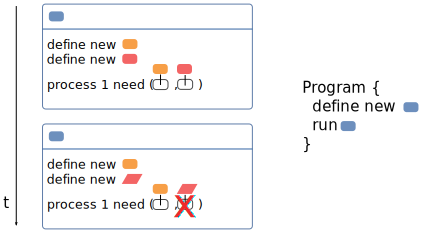
\includegraphics[width=.7\linewidth]{composants_principes_a.pdf}
  	\label{subfig_decouplage:a}}\qquad
  \subbottom[]{
	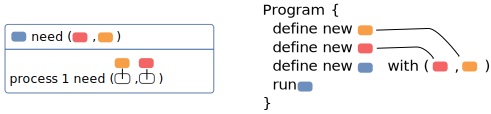
\includegraphics[width=.8\linewidth]{composants_principes_c.pdf}
  	\label{subfig_decouplage:b}}
  \subbottom[]{
	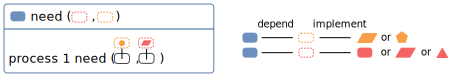
\includegraphics[width=.8\linewidth]{composants_principes_d.pdf}
  	\label{subfig_decouplage:c}}
 \end{sidecaption}
\end{figure}


Si on recontextualise ces principes à notre problèmatique, les classes de composants nécessaire à l'execution minimale d'un algorithme évolutionnaire dans MGO sont décrites dans la figure \ref{fig:cake_classe}, et s'appuie sur le travail déjà décrits de la communauté pour unifier la description des algorithmes.


\begin{figure}[!htbp]
	\begin{sidecaption}[fortoc]{Classe de composants nécessaires pour l'execution d'un EC.}[fig:cake_classe]
		\centering
		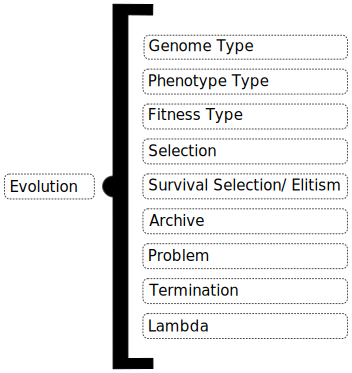
\includegraphics[width=0.7\linewidth]{cake_example.pdf}{
		}
  \end{sidecaption}
\end{figure}

Chacune de ces classes de composants est définit comme nécessaire pour le fonctionnement d'un algorithme d'évolution, dont la mise en dynamique du comportement générique est implémenté dans le composant Evolution. Tant que l'utilisateur n'aura pas fourni un composant compatible avec chacun de ces types de composants, alors le composant Evolution ne pourra pas s'executer. Le programme est définit comme un texte à trou, les boites sont bien placés, et le programme prêt à être executé suivant cet ordre, seulement ce n'est qu'un patron, une image, et cet ensemble de boite dont seule une partie de la logique à été intégré, doit encore être complété. C'est un peu comme un puzzle dans lequel il manque des pièces, vous devez soit créer de nouvelle pièces, soit retrouver les pièces qui respectent la forme de chaque trou pour que le puzzle soit de nouveau complet. 

L'inversion de controle détaillé dans les paragraphes précédents se matérialise de nouveau ici au travers du fait que c'est l'utilisateur qui définit sa composition, en s'assurant avec l'aide des instructions du programmes que les dépendances propres au fonctionnement de chacun des composants sont bien fournies. Tout programme ne remplissant pas les conditions renverra un message d'erreur à son execution. En ce sens MGO est probablement plus un \textit{framework} qu'une librairie logicielle \Anote{martin_fowler}. L'avantage d'une telle approche c'est que l'application peut être livrée avec un vaste catalogue de pièce correspondant à chaque emplacement, laissant à l'utilisateur la possibilité de choisir sa propre combinaisons, voire même de créer ses propres pièces si il estime quel sont manquantes. 

Ils existent différentes techniques pour que cette technique puisse être mise en oeuvre, mais en Scala, l'implémentation la plus courante et la plus utilisé est connu sous le nom de \foreignquote{english}{Cake Pattern}, \foreignquote{english}{Scalable Component Abstractions} ou encore \foreignquote{english}{Component Based Dependency Injection}, accessible nativement dans le langage car pensé et implémenté par son créateur Martin Odersky.

Le défaut de cette technique, c'est qu'il rend la lecture du code source plus difficile, du fait de ce morcellement dans l'appel des différentes fonctions.


\subsubsection{La mise en oeuvre du couplage MGO - openMOLE }

Le choix est fait ici de développé une librairie MGO utilisable de façon indépendante, ou de façon couplé à openMOLE. 

Les objectifs motivant la construction d'une nouvelle librairie sont les suivants : 



L'étape suivante est do nc le couplage de cette librairie avec openMOLE 


Martin Oderskys’


\begin{minted}[linenos=true,frame=single,fontsize=\footnotesize]{scala}
import fr.iscpif.mgo._
import math._
import util.Random

trait ZDT4 extends GAProblem with MGFitness {

  def min = Seq.fill(genomeSize)(0.0)
  def max = 1.0 :: Seq.fill(genomeSize - 1)(5.0)

  type P = Seq[Double]

  override def express(g: Seq[Double], rng: Random) = Seq(f1(g), f2(g))
  override def evaluate(p: P, rng: Random) = p

  def f1(x: Seq[Double]) = x(0)
  def f2(x: Seq[Double]) = g(x) * (1 - sqrt(x(0) / g(x)))
  def g(x: Seq[Double]) =
    1 + 10 * (genomeSize - 1) + (1 until genomeSize).map 
    { i => pow(x(i), 2) - 10 * cos(4 * Pi * x(i)) }.sum
}
}
\end{minted}

\section{Une brique logicielle dédiée à la visualisation de résultats}




%% -*- root: These.tex -*-

\section{SimpopLocal}
\label{sec:simpopLocal}

%% -*- root: These.tex -*-

\section{MicMac}
\label{sec:micmac}

\printbibliography[heading=subbibliography]

\appendix

\chapter{Historique du paradigme systémique}

\subsection{Retour sur la fondation et les apports du \enquote{paradigme systémique} au début du XXème siècle}
\label{ssec:systemique}

De la même façon que les épistémologues des sciences comme ici Olivier Orain \autocite{Orain2001}, l'auteur ne détaillera pas ici une approche inter-disciplinaire de la notion \footnote{Au sens donné par Piaget, voir note de bas de page \autocite {Orain2001}} de \enquote{système}, difficile à envisager dans un cadre global car sa diversité d'acceptation est fonction, d'une part de la rapide évolution de cette notion depuis les années 1940, et d'autre part la règle définissant l'acceptation de cette \textit{notion} dépend non seulement de la variabilité inter-disciplinaire, mais aussi intra-disciplinaire. Le terme \enquote{approche systémique} est alors proposé par \autocite{Orain2001} pour incarner cette diversité d'intégration par les disciplines des sciences sociales de la \enquote{théorie systémique} ou \enquote{systémique}.

La complexité d'approche caractéristique de cette notion est pour Jean Louis Lemoigne grandement lié à la reconstruction épistémologique \textit{a posteriori} de ce qu'il appelle \enquote{paradigme systémique}. Une acceptation qui parait d'autant plus justifié tant l'étude exhaustive de la ramification qui découle du concept est impossible, et sans rentrer dans les détails de querelles entre les différentes chapelles, il est acceptable de voir cette construction comme un processus de raffinement cumulatif. \hl{a dire mieux}

\subsubsection{La Cybernétique}
\label{ssubsec:cybernetic}

\paragraph{Des outils pour penser une nouvelle causalité}

Une des branches communément admises comme fondatrice du mouvement tient dans l'organisation des conférences de Macy entre 1942 à 1953. Celle ci sont considérés comme un des tout premier regroupement interdisciplinaire et marque une période de changement profond dans l'histoire des sciences en général, et particulièrement en science sociale. Celles ci vont réunir pendant plusieurs années autour d'une même table des acteurs majeurs des sciences physiques et sociales pour discuter autour de régularités communément observés, avec pour idée la construction d'un savoir commun que l'on pourra alors qualifier de trans-disciplinaire.

Les conférences naissent suite à la rencontre entre un mathématicien réputé au MIT N. Wiener, un neurobiologiste A. Rosenbluch, et un ingénieur électronicien J.Bigelow qui vont opérer un rapprochement entre l'homme et la machine entre 1942 et 1946 (pour rappel le premier ordinateur ENIAC est opérationel en 1946) par le biais de groupes inter-disciplinaires chargés d'explorer ce \textit{no man's land} à l'interface des deux disciplines.

Plusieurs \enquote{outils} dérivent de ces premiers séminaires organisés dès 1942 à la Josiah Macy, Jr. Foundation : la notion de \enquote{boite noire} ou système téléologique fonctionel, et la notion de \textit{feedback} ou causalité circulaire, avec pour objectif principal l'étude de l'homéostasie introduite auparavant par les travaux pionniers du physiologiste Walter Cannon en 1926.

Si la notion d'homéostasie pour des organismes vivants apparaît pour la première fois cité par Claude Bernard 1865, celle ci est reprise et étendue par Walter Cannon en 1932 dans le livre \textit{The Wisdom of the Body} \autocite{Cannon1932} comme « l’ensemble des processus organiques qui agissent pour maintenir l’état stationnaire de l’organisme, dans sa morphologie et dans ses conditions intérieures, en dépit de perturbations extérieures ». Ainsi dans le cadre de son application biologique cette rétro-action permet de décrire un certain nombre de mécanisme à l'oeuvre dans une cellule en interaction avec son environnement qui tente de maintenir de façon stable dans son milieu la concentration d'éléments comme les ions, la glycémie, etc.

L'attention des discutants dans ces premier séminaire porte donc avant tout sur l'ubiquité du concept et la pertinence de son transfert hors des systèmes biologiques. Wiener fait alors un rapprochement décisif entre les problématiques de calcul de trajectoire en balistique et des maladies nerveuses ayant pour symptôme l'ataxie. De ces discussions émergent alors un même schéma explicatif qui semble à la fois convenir à ces problématiques, la \enquote{causalité circulaire}. \autocite[774]{Pouvreau2013, Rosnay1975}

L'approche néo-béhavioriste retenue par les discutants \enquote{consiste à étudier un objet comme une \enquote{boite noire}, par l'examen de l'extrant de l'objet [i.e tout changement produit dans son environnement] et des relations entre cet extrant et l'intrant [i.e tout événement externe qui modifie l'objet]} \autocite{Pouvreau2013} En adoptant cette approche, le \enquote{comportement} d'une entité est perçu \enquote{comme tout changement extérieur détectable de cette entité par rapport à son environnement} , et par téléologique il faut entendre un comportement \enquote{finalisé} c'est à dire déterminé par un mécanisme de \enquote{rétroaction} négative. De la connaissance de ces entrants et de ces sortants, on peut en déduire qu'il existe une retro-action négative ou positive, ou \textit{feedback} permettant de décrire progressivement le système de commande de la boite noire.

L'introduction de cette \enquote{causalité circulaire} est pour l'époque loin d'être anodine car elle remet en cause le schéma classique linéaire cause \textrightarrow conséquence, qui se traduit dans le temps par la relation avant \textrightarrow après, la cause étant irrémédiablement suivi d'une conséquence. La possibilité de causalité circulaire, positive ou négative, brise ce schéma, et ne permet plus d'isoler un ordre entre cause et conséquence, c'est le problème de \enquote{la poule et de l'oeuf}. En réintroduisant la poursuite d'un but, on injecte une autonomie, une spontanéité, une dynamique entre objets qui était jusque là absente de la causalité linéaire déterministe.

Appliqué à un système servo-mécanique, la stabilité de celui-ci suppose la capacité à anticiper et à annuler les agressions extérieures par une capacité de régulation (flexibilité) qui repose plus alors sur la dynamique des interactions que sur la structure physique en place (rigidité), un mode de fonctionnement impossible si on se place dans le cadre de la \enquote{pensée classique} de l'époque.

%Dans "Behavior, Purpose and Teleology", le terme téléologie est à ce titre utilisé comme un synonyme de "l'objectif controllé par la rétroaction".\footnote{wikipedia}

\paragraph{La réintroduction du concept de \enquote{téléologie}}

Avec la mise en place d'une classification de ces comportements, et en prenant distance du concept de \enquote{causalité finale} qui lui était rattaché, les auteurs espèrent ainsi redorer le concept de téléologie, renouant avec la reconnaissance de l'\enquote{importance du but} qui avait disparu avec la mise au ban de ce concept. Reprenant les explications de \autocite[776]{Pouvreau2013}, celui-ci cite \autocite[23-24]{Rosenblueth1943} \enquote{[...] Puisque nous considérons la finalisation comme un concept nécessaire afin de comprendre certains modes de comportement, nous suggérons qu'une étude téléologique est utile si elle évite les problèmes de causalité et se limite à s'attacher à l'étude du but [...] Le comportement téléologique devient synonyme de comportement contrôlé par une rétroaction négative et gagne donc en précision par une connotation suffisamment restreinte.} La finalité est reintroduite via le concept de \enquote{téléologie}, mais elle est libéré de la notion de \enquote{causalité} qui lui était autrefois associé. Elle redevient l'étude des comportement associé à un but, dont l'importance ne peut plus être nié, et redevient compatible avec le concept autrefois opposé de déterminisme.\footnote{Pour donner un exemple peut-être plus parlant, l'étude en biologie des comportement oeuvrant dans la formation d'un organisme par une méthode téléologique n'empêche pas l'usage d'un cadre de pensée déterministe  correspondant à la formation d'un même organisme à partir d'un même code initial (un déterminisme largement remis en cause depuis, voir par exemple \href{http://www.nytimes.com/2014/01/21/science/seeing-x-chromosomes-in-a-new-light.html?ref=science&_r=0}{New York Times} )}

De ces discussions deux articles fondateurs à la fois des sciences cognitives \autocite[23]{Dupuy2000} et de la cybernétique vont être publiés : \textit{Behavior, Purpose and Teleology}ou Rosenblueth, Wiener, et Bigelow \enquote{ propose de déconstruire la distinction entre action volontaire et acte réflexe, en assimilant la volonté à un mécanisme de rétro-action (\textit{feedback})}; et \textit{A logical calculus of the ideas immanent in nervous activity} où McMulloch et Pitts donne \enquote{une base purement neuroanatomique et neurophysiologique au jugement synthétique \textit{à priori}, et de donner ainsi une neurologie de l'esprit}

\paragraph{ Les limites du transfert des concepts aux sciences sociales}

\subparagraph{Introduction aux sciences sociales}
Parmis les auteurs de ces premiers séminaires organisés entre 1942 et 1944 figurent deux représentant des sciences sociales, Gregory Bateson et Margaret Mead. Enthousiastes, il vont rapidement trouver dans l'étude des concepts développés dans ce premier séminaire (1942) un écho à leur propre travaux sur la dynamique sociale, la notion d'homéostasie n'étant qu'un nouveau mot permettant de rassembler des travaux existants déjà au fait de ces phénomènes. Cette mise au jour de problématiques commune entre le biologique et le mécanique permet d'envisager la construction d'un référentiel lui aussi commun; une prise de conscience qui va amener les auteurs du cercle de réflexion initial à envisager rapidement l'élargissement de celui-çi à l'ensemble des acteurs des sciences sociales.

La suite des conférences de Macy (1946-1952) sera organisés par Arturo Rosenbluch et son ami Warren McCulloch, un autre neurobiologiste. Cette ouverture vers les sciences sociales est timide dans un premier temps, et ce n'est qu'à la 2ème conférence en octobre 1946 sur une suggestion de Lazarsfeld que les conférences concrétise cette ouverture dans le cadre d'un sous séminaire intitulé \textit{Téléogical Mechanisms in Society}. La 4ème conférence acte cette ouverture et introduit pour la troisième fois de suite une modification de l'intitulé, avec cette fois ci l'adjonction d'une dimension sociale à un objet d'étude, qui apparaît encore à cette date difficile à définir : \enquote{la causalité circulaire et des mécanismes de \textit{feedback} dans les systèmes biologiques et sociaux}. Le terme \textit{Cybernetics} est pour la première fois introduit dans les séminaires par Wiener en 1946. Il faut toutefois attendre 1949 et la septième conférence pour que sous l'influence d'un nouveau participant nommé H. Von Foerster, ce terme chapeaute de façon définitive les prochains intitulés de séminaires. Au final, ces dix séminaires vont participer de l'émergence de la \enquote{science cybernétique} en \enquote{permettant l'échange effectif de savoir et d'experiences, tant entre les disciplines qu'entre les sciences et la société}, réalisant par là un des objectifs annoncé par Wiener et Rosenbluch dans leur classification, faisant de la cybernétique une \enquote{[...] science générale des systèmes à comportement finalisé ayant principalement pour objet ceux dont le comportements est \enquote{téléologique} } \autocite{Pouvreau2013}

\subparagraph{Des biais mécanisistes mettent en échec ce premier transfert}

Wiener mais aussi d'autre acteurs de la cybernétique ont vus assez tôt tout l'intérêt que pourrait apporter l'utilisation et le transfert d'outils comme \enquote{la boite noire}, ou le principe de régulation par \enquote{rétro-action} une fois appliqué à l'étude des interactions dans les systèmes sociaux. Mais les difficultés d'applications et les critiques ont rapidement mis à mal cet objectif trans-disciplinaire, pour plusieurs raisons qui tiennent : d'une part à l'existence de restriction mathématiques remettant en cause la scientificité des résultats obtenus : (a) les statistiques sur le long terme étant difficile à obtenir (b) la difficulté à minimiser la distance entre observateur et phénomène observés, et donc le biais qui s'applique aux données dans un tel cadre; et d'autres part au réductionnisme et le biais mécanicistes touchant la vision de certains acteurs des conférences de Macy  : \enquote{[...] la vie était pensée comme un dispositif de réduction d'entropie ; les organismes et leur associations, en particulier les hommes et leurs sociétés, l'étaient comme des servomécanismes ; et le cerveau comme un ordinateur} \autocite[784]{Pouvreau2013}

\autocite[782]{Pouvreau2013} explique très bien les limitations qui font  de l'extension de la cybernétique au sciences humaines une simple \enquote{[...] ressemblance superficielle au niveau du formalisme. Ne serait-ce que parce que dans un système tel que conçu par la \enquote{première} cybernétique, par définition fermé à l'information, la téléologie ne peut qu'être confinée au cercle d'un but déterminé; et que pour cette raison, ce modèle ne permet pas de comprendre de quelle manière un système peut être amené à redéfinir ses buts à partir de ses interactions avec son environnement, la pertinence d'une téléologie relative à des buts \textit{intentionels} restant donc intacte en sciences humaines}.

\subsubsection{La GST ou la théorie des \enquote{systèmes ouverts}}
\label{ssubsec:gst}

Cette incapacité de la première cybernétique à coller aux problématique des systèmes sociaux va trouver un écho plus positif dans un courant qui se développe en parallèle du mouvement cybernétique. Ce mouvement fondé par le biologiste Ludwig Von Bertalanffy en 1937 peut être considéré comme la deuxième branche venant enrichir le paradigme systémique. Tout en apportant de nouveaux concepts, celui ci va se positionner de façon critique par rapport à la \enquote{première cybernétique} tout en englobant par la suite les autres innovations qui proviendront de ce courant, Asbhy jouant le rôle important de médiateur entre ces deux courants.\autocite[]{Pouvreau2013} De cette prise de position va peu à peu découler la construction d'une théorie établissant une méthodologie logico-mathématique à vocation unifiante, accessible à n'importe quel champs disciplinaire pour décrire les lois de structure similaires (isomorphe). \autocite{LeMoigne2006a}.

Ainsi rapporté par LeMoigne en 1977, cette \enquote{vision stupéfiante est celle d'une une théorie générale de l'univers, du système universel} \autocite[59]{Lemoigne1977}. Le mot \enquote{Vision} est ici quasi synonyme de \enquote{Révélation}, car elle amène à voir une tout autre approche du réel pour qui s'en rapporte. Ainsi selon les mots même de Bertalanffy, \enquote{De tout ce qui précède se dégage une vision stupéfiante, la perspective d'une conception unitaire du monde jusque-là insoupçonnée. Que l'on ait affaire aux objets inanimés, aux organismes, aux processus mentaux ou aux groupes sociaux, partout des principes généraux semblables émergent} \autocite[59]{Lemoigne1977} \autocite[220]{Bertalanffy1949}. Une idée déjà existante dans la maxime célèbre de Claude Bernard en 1885, remise au gout du jour par \autocite{Lemoigne1977}, celle-ci résume toute la souplesse offerte par cette notion d'un point de vue de la modélisation :  \enquote{Les systèmes ne sont pas dans la nature mais dans l'esprit des hommes}

Cette théorie nommé \textit{General System Theory} (GST) est évoqué pour la première fois en public en 1937-38 par Bertalanffy, s'ensuit alors la rédaction d'une première ébauche en 1950, et il faudra attendre 1968 pour qu'un ouvrage titré \textit{General System theory: Foundations, Development, Applications} proposent une synthèse de toutes les avancées. La durée de développement de cette théorie n'est pas anodine, et si on en croit Pouvreau \autocite{Pouvreau2013} qui a analysé en détail la très vaste littérature associé à cette thématique, cette théorie n'en est pas vraiment une en réalité. En effet l'état inachevé du projet de Bertanlanfy laisse plus à penser qu'il s'agit là d'un \enquote{projet}, et c'est à ce titre que Pouvreau préfère employer le terme de \enquote{systémologie générale} pour désigner ce qu'il définit alors comme \enquote{le \textit{projet} d'une \textit{science de l'interprétation systémique} du \enquote{réel} } \autocite[9]{Pouvreau2013}. L'hypothèse défendu par Pouvreau étant que cette \enquote{[...]science de l'interprétation systémique du \enquote{réel} se caractérise en fin de compte comme une herméneutique, au sens où elle a pour vocation d'élaborer à la fois les moyens de construire des interprétations systémiques d'aspects particulier du \enquote{réel} sous la forme de modèles théoriques spécifiques et les moyens d'interpréter à leur tour de tels modèles comme des déclinaisons de modèles systémiques théoriques d'un degré de généralité supérieur.}\autocite[9-10]{Pouvreau2013}

Mais avant de même de fonder ce projet unifiant qui par la suite va rayonner et être absorbé (non pas sans déformation ..) dans un grand nombre de disciplines, dont la géographie, il est intéressant de rappeler comment la théorie biologique de Bertalanffy a participé de la formation de grandes notions comme l'\enquote{équifinalité} ou l'\enquote{auto-organisation}, des notions aujourd'hui communément admises comme fondatrice du paradigme actuel de la \enquote{complexité}.

Bertalanffy poursuivant depuis 1937 avant tout cet objectif de dépasser la compréhension des systèmes biologiques  englué jusque alors dans une dualité opposant les \enquote{vitalistes} et \enquote{mécanistes}. La synthèse de ces travaux est organisé dans une \enquote{biologie organismique} qui fonde une troisième voie visant d'une certaine manière la réconciliation entre les deux approches \autocite[55-56]{Lemoigne1977} \autocite[258]{Bertalanffy1949}. Avec cette nouvelle biologie théorique il s'agissait donc d'incarner \enquote{l'avenir de la biologie" en établissant via la mobilisation de moyen scientifique (analyse et analogies physico-chimique et mathématique du vivant) écartant la métaphysique/psychiques, un programme de recherche des \enquote{loi systémiques ou d'organisation à tous les niveaux de la nature vivante} entendues comme \enquote{l'explication de l'harmonie et de la coordination des processus à partir de la dynamiques des forces qui leur sont immanentes}}\autocite[456]{Pouvreau2013}. Principalement \enquote{ordonnées en direction de la conservation de la totalité}\autocite[440-458]{Pouvreau2013} dans une \enquote{tendance à une complication croissante}, cette \enquote{Gestalt organique} de la théorie \enquote{organismique} de Bertalanffy place \enquote{l'Organisation} des processus comme une véritable problématique de recherche, et met de coté la question de la \enquote{finalité} du vivant.\autocite[455-457]{Pouvreau2013}

Déjà tout à fait conscient que \enquote{le tout est plus que la somme des parties} Bertalanffy admet que l'étude des mécanismes physico-chimiques des processus vitaux tient plus d'une heuristique de recherche, une \enquote{méthode téléologique qui permet \enquote{d'examiner jusqu’à quel point le caractère de conservation de la totalité se manifeste dans les processus qui se déroulent en eux}} sans jamais arriver à en donner une complète description.\autocite[464]{Pouvreau2013}

Cette \enquote{biologie théorique organismique} (également appelé de façon synonyme par Bertalanffy \enquote{théorie systémique du vivant}) montre en bien des points toutes les prémisses d'une pensée systémiste et non réductionniste qui dépasse déjà largement le cadre seul de la biologie, et cela même avant 1937 et l'introduction de \enquote{systèmes ouvert} \autocite[499]{Pouvreau2013} qui ont fait la renommée de l'auteur.  Cette \enquote{biologie organismique} de Bertalanffy, bien évidemment construite sur les acquis et l'aide de bien d'autres de ces contemporains (voir \autocite{Pouvreau2013}, arrive à maturité en 1937 \autocite[14]{Pouvreau2013}, et présente déjà à ce stade tout les traits d'une première \enquote{systémologie restreinte}, qui va servir d'\enquote{antichambre} à la formation de la future \enquote{systémologie générale} (la première évocation publique date de 1945, mais des traces indirectes de ses premiers discours semblent remonter à 1937).\autocite[670]{Pouvreau2013} de Bertalanffy.

% D'abord on fait le point sur les principes (ce qui suppose de faire une grosse parenthèse avec tout ce que l'on a décrit sur la thermodynamique) et ensuite on peut passer à la critique, évoquant l'équifinalité et la hierarchisation de processus qui permet de recentrer aussi l'étude des boites noires.

L'articulation entre les deux \enquote{principes organismiques} qui fondent sa théorie apparaît de façon très claire dans une première définition du vivant en 1932, ici cité dans sa version telle que raffinée par Bertalanffy en 1937, date à laquelle selon

%Définition des deux principes organismiques !?

Le premier principe théorique \enquote{organismique} de Bertallanfy s'appuie sur le principe biologique fondamental qu'il a énoncé dès 1929 avec la \enquote{conservation du système organique en équilibre dynamique}. Un équilibre qui parait statique d'un point de vue extérieur, mais qui est en réalité dynamique car son existence même est basé sur la remise en jeu permanente d'une partie du travail effectué par la cellule pour maintenir le système organique loin de l'équilibre \enquote{vrai} (physique, c'est à dire celui qui correspond à une mort thermique, ou chimique qui ne peut pas produire non plus de travail à l'équilibre). Un \enquote{équilibre de flux} qui ne peut être réalisé que parce que l'organisme n'est ni un système fermé, ni un système statique, mais un système dont l'ordre et l'organisation (def à valider ici) est fondé sur un travail issue d'un \enquote{flux} de matière et d'énergie résultat d'une transaction à double sens avec son environnement. \autocite[472]{Pouvreau2013} Je me permettrai de citer ici Morin, qui reprenant Héraclite, évoque très bien cet antagonisme à l'oeuvre dans les systèmes organiques, mais aussi par extension sociaux \enquote{Vivre de mort, mourir de vie} : \enquote{ ne vivons-nous pas de la mort de nos cellules qui vieillissent et se décomposent pour laisser la place à des cellules jeunes ? [...] La vie et la mort sont certes deux ennemies fondamentales, mais la vie lutte contre la mort en utilisant la mort. Néanmoins, il est tuant de se régénérer en permanence. C’est épuisant. Finalement, on mveurt à force de rajeunir. On meurt de vie. } \autocite{MorinXX}

% Critique cybernétique
Le principe d'\enquote{équilibre des flux}, même si il peut être rapproché du concept d'\enquote{homéostasie} définit par les tenants de la \enquote{première Cybernétique} (en analogie avec les systèmes mécaniques) comme la \enquote{conjonction des processus par lesquels, nous autres, être vivants, résistons au courant général de corruption et de dégénérescence} est trop généraliste pour application en tant que tel à toute les notions de régulations organiques. \autocite[194]{Morin1977} \autocite{Wiener1950}. L'\enquote{homéostasie} tel que définit par Wiener dans le cadre de la Cybernétique s'avère en réalité être un mécanisme de régulation organique parmi tant d'autres, tous n'étant pas basé sur le schème de rétro-action. A ce titre, la notion d'\enquote{homéostasie} pourtant quasi semblable dans sa définition à l'équilibre de flux dans un système ouvert, mobilise en réalité un tout autre fonctionnement que le schème de rétro-action Cybernétique, et tient plus de l'extension aux systèmes ouverts du principe dit de \enquote{Le Chatelier}. De la même façon la régulation intervenant dans le processus de croissance des organismes qui nécessite la régénération, et l'évolution des structures dans le temps n'est pas compatible avec l'ordre structural pré-établi des machines et le scheme de rétro-action promis par la Cybernétique. La vision \enquote{machinaliste} limité/biaisé des premiers cybernéticiens n'est donc pas satisfaisante pour une application aux systèmes organiques, dès lors qu'il faut accepter la constance non pas des structures mais des interactions entre les structures. Bertalanffy développe une classification plus complète de ces régulations qu'il considère selon le type de leur téléologie, et introduit le concept d'\enquote{équifinalité} comme téléologie dynamique moteur dans la construction et le maintien des systèmes organiques. Dans ce contexte, le principe d'équifinalité \autocite[131]{Pouvreau2013}, est ainsi évoqué pour la première fois comme la possibilité d'atteindre le même état finalisé à partir de trajectoires quelconques, un processus impossible dans le cadre de système fermé où les condition initiales définissent par avance l'état final. Ce faisant, Bertalanffy introduit la primauté de l'ordre dynamique sur l'ordre structurel et fait de l'équifinalité un concept qui dérive de l'ouverture des systèmes. \autocite[489]{Pouvreau2013} \autocite[647]{Pouvreau2013} Un exemple illustrant les effets de l'équifinalité dans les organismes vivants peut être montré avec le processus de division embryonnaire. Ainsi un organisme a qui ont impose la fragmentation, la régénération, ou des blessures d'unités biologiques élémentaires comme les gènes ou les chromosomes va de façon constante s'organiser suivant un plan pré-établi menant à la \enquote{constitution d'un tout}, autrement dit un organisme complet.

%Il nécessite un autre mode d'explication de processus téléologique, celui de la cybernétique s'avérant incompétent au regard du principe d'équifinalité observé dans les systèmes organiques.

% Bertalanffy s'appuie dans sa critique à raffiner sa classification des téléologies, ce qui lui permet d'introduire le concept d'équifinalité comme sous-type de téléologie dynamique, un type de processus de régulation qui selon lui ne peut pas être expliqué par les schèmes cybernétique initiaux, seulement capable de mobiliser le concept de finalité en regard d'une explication basé sur un arrangement structural pré-établi (une machine faites de composants) et non pas l'ordre  dynamique propres au système en équilibre de flux.

La combinaison des deux principes \enquote{organismique} menant à la théorie des \enquote{système ouvert en équilibre de flux} deux heuristiques de recherches \autocite[481]{Pouvreau2013}:
\begin{itemize}
\item La subordination du \enquote{principe de hierarchisation} à celui du \enquote{système ouvert en équilibre de flux}, autrement dit la genèse et le maintien de l’ordre hiérarchique d’un \enquote{système organique} est conditionné par l'existence d'un \enquote{système ouvert en équilibre de flux}
\item  La relation précédente est un principe ubiquitaire s’appliquant à tous ses niveaux
\end{itemize}

Cet idée sera particulièrement fructueuses une fois articulé avec le principe d'un enboitement des systèmes, l'accroissement du degré de liberté dans un système résultant de l'équifinalité.
 \autocite[38]{Bertalanffy1973} \autocite[786-788]{Pouvreau2013}

%Developpement rendu possible uniquement par l'apport des théories de la thermodynamique ... l'expression d'une trajectoire indépendamment de l'état final, celui ci n'est qu'un processus de régulation parmis d'autres, car ce même système organique est non seulement capable de maintenir son état mais choses plus importante, il permet surtout de produire de l'organisation, de la complexification.

% Relation avec science sociale ??
% => entéléchie /
Cette notion d'équifinalité reliant un niveau micro à un niveau macro pourra par la suite être transposé dans les système sociaux, le parallèle de l'individu comme acteur réflexif dans la société sera mobilisé par ?

De ce fait la Cybernétique n'est pour Bertalanffy qu'un cas particulier dans une systémologie dont il pense qu'elle peut être beaucoup plus universelle... ++ Homéostasie avec Ashby ? ++

Tel que définie, cette notion d'équilibre dynamique de Bertalanffy est bien différente de celle produites en physique et en chimie, qui se caractérise justement par l'absence de travail disponible, l'énergie disponible étant minimale. Pour que la permanence d'un ordre puisse être effective dans la théorie organismique, il faut qu'il y ai un échange, un flux d'énergie mais aussi de matière possible avec l'environnement; une différenciation qui amène Bertalanffy à développer dès 1937 une théorie des \enquote{systèmes ouverts}, la seule capable de s'appliquer également à des systèmes sociaux par la suite.

% Sur l'ouverture des systèmes
Pour mieux comprendre en quoi cette ouverture est importante pour l'application du paradigme systémique aux sciences sociales, il faut revenir quelques décennies en arrière pour définir les limitations des premier systèmes issue de la thermodynamiques, limitations qui par la suite ont irrigués les réflexions initiales des cybernéticiens tout autant que les motivations de Bertalanffy pour les dépasser dans le cadre de sa théorie \enquote{organismique}

La seconde loi de la thermodynamique esquissé par Carnot et formulé par Clausius en 1850 montre que l'energie calorifique ne peut se reconvertir, elle se \textit{dégrade} et perd son aptitude à effectuer un \textit{travail}. Clausius nomme \enquote{entropie} cette diminution irréversible de l'aptitude à se transformer et à effectuer un travail, propre à la chaleur.\autocite[35]{Morin1977} Prigogine dans la \textit{fin des certitudes} écrit à propos de l'entropie qu'elle \enquote{[...] est l’élément essentiel introduit par la thermodynamique, la science des processus irréversibles, c’est-à-dire orientés dans le temps.}

C'est Boltzmann, Gibbs et Planck qui vont par la suite faire le lien entre le niveau micro des particules et la notion de chaleur. Parce que la chaleur est caractérisé par l'agitation désordonné des molécules dans un systèmes, l'entropie devient plus qu'une simple réduction du travail, c'est aussi l'ordre et le désordre des molécules qui en est la cause. Cette transformation s'effectue avec création d'entropie, une \enquote{quantité de désordre} qui ne peut que croître dans le temps et cela jusqu'à atteindre une valeur maximale équivalente à ce nouvel état d'équilibre. De ce fait et de façon générale celle-ci définit comme évolution irréversible toute transformation réelle dans un système isolé (Système où la frontière est totalement imperméable : l'Univers est par définition un tout englobant) ou fermé (Système ou la frontière est perméable aux flux entrant ou sortant d'énergie mais imperméable aux échanges de matière : La Terre reçoit de l'énergie du soleil) partant d'un état non stable et se dirigeant vers un nouvel état stable.  Ainsi si on considère l'univers comme un méta-système isolé englobant tout les autres, alors ce second principe a pour corollaire que l'entropie de l'univers augmente vers un état de désordre maximal qui se traduit en définitive par une mort thermique.

L'intuition de cette possible analogie entre loi gouvernant systèmes physiques et biologiques est issues des réflexions menés par Boltzman, qui comme ces contemporains du XIX siècle est admiratif pour la récente théorie évolutive de Darwin \autocite[27]{Prigogine1996}. Celui ci tente alors un parallèle avec ses propres travaux sur la seconde loi de thermodynamique, que l'on retrouve dans une des fameuses citations présente dans son livre \enquote{second law of thermodynamic} : \enquote{ The general struggle for existence of living beings is therefore not a struggle for raw materials — the raw materials of all organisms in the air, water and soil are in abundance there — nor about energy, which in the form of heat, unfortunately, is contained abundantly [but unfortunately] [in]convertible in each body, but a struggle for entropy, which is available [disposable] by the transfer of energy from the hot sun to the cold earth.}

% Le sys ouvert/fermé , de la thermodynamique à la biologie ?
Le point de vue de Boltzmann est repris et théorisé par Alfred J. Lotka, un mathématicien, chimiste et statisticien qui va largement influencé par la suite Bertalanffy dans la formation de sa \enquote{systèmologie générale} \autocite[178]{Pouvreau2013} par ces études de la démographie des populations et des flux de matières dans le monde biologiques \autocite[545-546]{Pouvreau2013} , toutes deux usant largement des équations différentielles (un premisse d'isomorphisme mathématique applicable à diverses disciplines pour qui quiconque tente de rentrer dans le formalisme de Lotka, et par la suite Lotka et Volterra \autocite[550]{Pouvreau2013}). De la même façon que Bertalanffy par la suite, celui ci ignore sciemment les débats entre \enquote{vitalistes} et \enquote{mécanicistes}, et adopte un point de vue unificateur qui vise la réconciliation entre système physique et système biologique, et part à la recherche d'isomorphisme en s'appuyant sur le processus d'irréversibilité commun aux deux paradigmes : \enquote{[...] the law of evolution is the law of irreversible transformation; that the \textit{direction} of evolution [...] is the direction of irreversible transformations. And this direction the physicist can define or describe in exact terms. For an isolated system, it is the direction of increasing entropy.  The law of evolution is, in this sense, the second law of thermodynamics} \autocite[26]{Lotka1925}.

Dès 1922 \autocite{Lotka1922a} \autocite{Lotka1922b} Lotka une nouvelle théorie qui acte la capacité de capturer de l'énergie comme un optimum à atteindre guidant la sélection tel quel est décrite par l'évolution Darwinienne. Il est également l'un des premier à percevoir les limites des lois actuelle de la thermodynamiques pour expliquer les processus du vivants, ainsi \enquote{Tenant pour légitime de traiter les êtres vivants et leurs associations comme des systèmes physiques, Lotka insistait toutefois sur le fait qu’il s’agit de « systèmes ouverts » aux flux de matière et d’énergie (ainsi que Raymond Defay (en 1929) et Bertalanffy (en 1932) les qualifièrent plus tard), capables d’échapper à l’équilibre thermodynamique défini par un maximum d’entropie promis aux systèmes fermés par le Second Principe, et d’évoluer vers une structuration croissante.} \autocite[179]{Pouvreau2013}

En effet pour un système vivant, l'état d'équilibre tel que décrit pour des systèmes clos ou isolé, correspond à un état de mort cellulaire. Hors, il est prouvé empiriquement à cette période que les systèmes vivants évolue dans un environnement chimique en perpétuel évolution loin de l'équilibre, et sont de fait capable de maintenir un haut niveau d'organisation par l'échange d'énergie et de matière avec l'environnement. Autrement dit, il n'est pas possible de concevoir l'équilibration permanente des systèmes vivants comme le résultat d'une évolution entropique croissante \autocite[248]{Lemoigne1977}. Des résultats énoncés sous forme de loi en 1929 par Bertallanfy, qui fait de \enquote{la conservation de système organique en équilibre dynamique} un \enquote{principe biologique fondamental}, et qui deviendra plus tard dans sa théorie \enquote{organismique}, le premier principe de  \enquote{système ouvert} en \enquote{équilibre de flux}. \autocite[492]{Pouvreau2013}

Mais en voulant faire l'analogie entre ces deux systèmes, une question va rapidement se poser aux scientifiques. \enquote{Comment la progression irréversible du désordre pouvait elle être compatible avec le développement organisateur de l'univers matériel, puis de la vie, qui conduit à homo sapiens ?}, une question qui va engendrer la problématisation et un changement de point de vue radical. Comme le résume bien \textit{a posteriori} Morin dans son premier tome de \textit{La Méthode}, \enquote{A partir du moment où il est posé que les états d'ordre et d'organisation sont non seulement dégradables, mais improbables, l'évidence ontologique de l'ordre et de l'organisation se trouve renversée. Le problème n'est plus : pourquoi y a-t-il du désordre dans l'univers bien qu'il y règne l'ordre universel ? C'est : pourquoi y a-t-il de l'ordre et de l'organisation dans l'univers ? } \autocite[37]{Morin1977}

Avec de tel propos se pose alors rapidement la question des mécanismes à l'oeuvre dans le vivant qui permettrait en quelque sorte de rétablir l'universalité de la seconde loi thermodynamique. Bien qu'intuité par de nombreux chercheur comme Lotka ou Bertalanffy, il faudra attendre les années 1940 pour que s'amorce plus concrétement ce rapprochement entre paradigme évolutionniste et domaine de la thermodynamique, concrétisé par le partage des théories entre biologistes et physiciens, qui va se réaliser notamment sous le couvert des récents progrès de ce dernier, permettant l'émission de nouvelle hypothèses.

Reprenant l'acceptation d'un système ouvert, c'est le livre \textit{What is Life} de Schrödinger (1944) qui va marquer le plus les esprits, et soulève le mieux ce paradoxe à la croisée des deux théories. Deux choses au moins fascine celui-ci \autocite{Foerster1959}, d'une part l'existence d'un code héréditaire qui définit au niveau micro la formation, l'organisation d'organisme au niveau macro (le principe \enquote{order-from-order}), d'autre part l'étonnante stabilité de ce code héréditaire immergé à 310 Kelvin \autocite[47]{Schrodinger1944}, et qui ne répond donc pas au fameux principe statistique \enquote{order-from-disorder} établit précédemment par Boltzmann.

En inscrivant comme nécessaire l'existence d'un code génétique comme un plan guidant l'évolution (tout comme Bertalanffy qui développe des théories similaires à la même époque), il introduit avec son concept de d'"entropie négative" un principe qui rend de nouveau compatible la seconde loi de thermodynamique avec l'évolution des systèmes biologiques : \enquote{le physicien attribuait le maintien de l’organisme dans un état \enquote{ stationnaire } éloigné de l’équilibre vrai à sa capacité de se \enquote{ nourrir } d’\enquote{ entropie négative } grâce à son ouverture sur son environnement. Une \enquote{ néguentropie } interprétée comme une \enquote{ création d’ordre à partir d’ordre } -- l’organisme créant un ordre spécifique à partir de la matière déjà ordonnée, structurée d’une manière déterminée mais devant être transformée pour ses besoins énergétiques, qu’il trouve dans son environnement} \autocite[502]{Pouvreau2013} Autrement dit, le maintien de l'organisation est un équilibre dynamique, un jeu à somme nulle où la création d'entropie est annulé par la capacité des organismes à transformer l'énergie, l'ordre puisé dans l'environnement pour maintenir ce degré d'organisation, un processus qualifié de néguentropique. Ce concept, déjà difficile à accepter tel quel dans sa généralité \autocite[225]{Lemoigne1977} va par la suite être raccroché à théorie de l'information de Shannon après son introduction en 1948 dans le microcosme Cybernétique. L'introduction de cette théorie étant un autre moment fort (avec la thermodynamique) ayant inspiré de nombreux développement dans la cybernétique. Mais les tentatives d'unification entre les deux théories débouche sur deux rapprochement possible, avec d'une part la qualification d'une \enquote{information pensé comme quantité physique} ou d'autre part l'expression des \enquote{quantité physique pensé comme de l'information}, selon que l'on adopte le point de vue de Wiener ou de Brilloin 1956 (auteur de la néguentropie qui associe qui associe \enquote{information} et principe de négentropie ). Ces points de vues font encore à l'heure actuelle l'objet de nombreux débats, certains voyant la physique de l'information comme un point de départ à creuser pour appeller une théorie de l'"organisation" \autocite[37-38]{Morin2005}, alors que d'autres n'y voient qu'un concept flou seulement basé sur la similitude des deux formules. Autant de ramifications naissent de ces positions, et leur présentation dépassent de loin le seul cadre d'étude de cette thèse, mais le lecteur pourra se référer au travail de \autocite{Triclot2007} pour mieux comprendre le point de départ d'un malentendu qui dure toujours /footnote{Voir par exemple la différence de ton qui existe entre le site http://www.eoht.info/page/Information+theory, mais aussi les notes de bas de pages de \autocite[277]{Lemoigne1977} }.

\autocite[482]{Pouvreau2013} Mais finalement plus que les idées développés par Shrödinger, la plupart étant déjà largement sous entendu dans les travaux des biologistes de l'époque, il semblerait plutôt que cela soit avant tout ce nouvel éclairage physiciste apporté à la biologie {REF}, et l'espoir déguisé (finalement non réalisé) de trouver de nouvelles lois physique à l'oeuvre dans la construction du vivant associé à la grande diffusion du petit livre dans le grand public qui amèna peut être de nombreux physiciens à ne plus ignorer les avancés dans ce domaine, notamment durant les années 1940 / 50, tel que Prigogine \autocite[77]{Prigogine1996}, Von Foerster, etc. \autocite[73]{Lemoigne1977}

Mais conscient des manquements et des reproches faites à son approche, alors incomplète, car focalisé sur la cinétique, celle ci n'est pas relié à une théorie plus explicatives sur les mécanismes energétiques à l'oeuvre justifiant l'existence de ces propriétés des systèmes vivants dans le cadre des systèmes ouverts. C'est les récents développements sur la \enquote{Thermodynamique des processus irréversibles} qui va introduire a posteriori la possibilité d'une thermodynamique des systèmes ouverts compatible avec l'approche de Bertlanffy. Des physiciens ayant participé à ces travaux sur la thermodynamique des systèmes ouverts loin de l'équilibre (Osanger, etc.) c'est les travaux de Prigogine  en 1946 \autocite{Prigogine1946} qui vont le plus attirer l'attention de Bertalanffy. Lorsque celui ci découvre vers 1948 ces récentes avancées qui semble faire parfaitement écho à ces travaux ( Prigogine n'hésitant pas à citer Bertalanffy comme un de ses modèles d'inspiration \autocite{Prigogine1996}), le rapprochement se fait assez rapidement et Bertalanffy n'hésite pas à promouvoir cette nouvelle thermodynamique comme le parfait support physique justifiant des principes qu'il a établi dans sa propre théorie des système ouvert en équilibre des flux ! \autocite[653-658]{Pouvreau2013}

Pas étonnant donc de voir Bertallanffy s'appuie sur les écrits de Schrödinger pour re-formuler et préciser ses premières intuitions,
+

Malheureusement le \enquote{théorème de Prigogine} de \enquote{minimum de production d'entropie} ne s'exprime que dans des conditions semblent il très drastiques \autocite[53]{Lebon2008} et limité à des systèmes très proche d'un état d'équilibre tel que le prouve les travaux de Denbigh : \enquote{ It is possible that certain reactions in biological systems may be sufficiently close to equilibrium for the rate of entropy production due to them to be very small. But in general it seems that the notion of minimum entropy production has no real significance as applied to chemical reaction in open systems [...] it is incorrect to regard the tendency of an open system to approach a stationary state as being determined by thermodynamic factors. The stationary state may or may not coincide with a state of minimum entropy production, according to whether the rates of the individual processes are linear functions of thermodynamic variables. In the above we have assumed this to be the case for diffusion (eqn. (ll)), but it is known not to be true for chemical reaction.} \autocite{Denbigh1952}

Hors l'état des systèmes biologiques est semble t il loin d'être proche d'un état d'équilibre thermodynamique.. Bertalanffy qui jusqu'à présent se contentait de relier les résultats à son programme organismique ne cache alors plus sa déception lorsque en 1953 il écrit \enquote{Un minimun de production d'entropie ne caractérise donc pas l'équilibre des flux dans les systèmes ouverts [...]}; autrement dit \enquote{la thermodynamique [...] ne nous dit jamais ce qui peut se passer dans un système, ce qui est permis [...] Et le problème de l'organisation progressive, la tendance néguentropique de l'évolution des organismes simples aux organismes compliqués, reste à présent non résolu.} Bien qu'ils n'abandonne pas l'idée de voir expliquer un jour sa théorie organismique par une théorie thermodynamique adapté, il abandonne en 1953 l'étude de la biophysique des systèmes ouverts et se consacre par la suite uniquement à la construction de sa théorie du système général.

Le fait est qu'il y a réduction d'entropie dans les systèmes en équilibre de flux, et qu'il y a maintient et augmentation du niveau d'organisation, sans que l'on sache pourquoi pour le moment dans le monde du vivant. Si l'analogie et le pont entre tissé entre physique et biologie semble donc encore soumis à questionnement, les travaux de Prigogine sur la thermodynamique des systèmes ouverts va continuer quand a elle à ouvrir bien d'autres perspectives, notamment dans les systèmes sociaux.

%paragraphe dimension reflexive auto-orga ...
Elle dépasser largement ce cadre, et appuie sur des bases physiques le concept d'"auto-organisation", une notion déjà introduite dans le mouvement cybernétique par Ashby, un homme clef dans la convergence des idées entre Cybernétique et GST.

Ashby, tout comme Von Foerster interviennent dans la création de la seconde cybernétique, et introduise une dimension réflexive aux débats.

Inspiré par Von Foerster, vont alors introduire un autre concept \enquote{d'order from noise}, totalement différent du \enquote{order-from-disorder} de Schrodinger.

TODO : Partie plus axé sur les changements de causalité ? (vient avant ou apres ici ?)

L'équifinalité

Un autre concept important est introduit par Ashby dans le mouvement Cybernétique, le concept d'auto-organisation, l'introduction du mot \enquote{auto} amorcant ainsi un virage réflexif qui annonce la seconde Cybernétique, piloté par Von Foerster.


%Des auteurs comme Prigogine en 1947 >> clairement inspiré par bertalanffy/ Schrodinger...  cf Pouvreau et internet
%Il fait le lien avec processus physique =>
%http://www.informationphilosopher.com/solutions/scientists/prigogine/
%http://www.informationphilosopher.com/solutions/scientists/schrodinger/

%http://en.wikipedia.org/wiki/Entropy_%28information_theory%29#Relationship_to_thermodynamic_entropy

C'est également à cette époque, que relayant les premiers travaux de Prigogine sur les systèmes dissipatifs, Bertalanffy va catalyser ainsi ces idées dans sa GST.

Ce procédé sera transféré au réel par Ashby, un autre cybernéticien qui travaillera dès 1946 à la mise au point d'une machine expérimentale capable de reproduire de façon mécanique cette dynamique de stabilisation face aux variations de son environnements. Nommé \enquote{homéostat} celle çi sera construite en 1948, et présenté aux conférences de Macy en 1952.

WIkipedia => L'implication de la cybernétique dans la systémique est historiquement plus liée au « deuxième mouvement cybernétique ». En effet, si selon Norbert Wiener la cybernétique étudie exclusivement les échanges d'information (car c'est « ce qui dirige » les logiques des éléments communicants d'où le mot cybernétique), dans son évolution qui engendrera la systémique, on réintègre les caractéristiques des composantes du système, et on reconsidère les échanges d'énergie et de matière indépendamment des échanges d'information.

La dégradation de l'énergie nécessaire pour maintenir une organisation implique l'irréversibilité des transformations.


The history of an open system is part of its structure, and Prigogine links open systems to irreversibility. Prigogine calls open systems dissipative. Put more simply, this means that matter does not tend to organise itself in a particular location unless there is some external energy source powering it. Evolution can be seen as matter organising itself.


The term \enquote{self-organizing} was introduced to contemporary science in 1947 by the psychiatrist and engineer W. Ross Ashby.[9] It was taken up by the cyberneticians Heinz von Foerster, Gordon Pask, Stafford Beer and Norbert Wiener himself in the second edition of his \enquote{Cybernetics: or Control and Communication in the Animal and the Machine} (MIT Press 1961).

Self-organization as a word and concept was used by those associated with general systems theory in the 1960s, but did not become commonplace in the scientific literature until its adoption by physicists and researchers in the field of complex systems in the 1970s and 1980s.[10] After Ilya Prigogine's 1977 Nobel Prize, the thermodynamic concept of self-organization received some attention of the public, and scientific researchers started to migrate from the cybernetic view to the thermodynamic view. WIKIPEDIA


Malgré les critiques soulevés de part et d'autres, du faite entre autre d'un objectif peut être un peu sur-évalué voire immodeste, celle ci aura un large écho auprès des sciences humaines, et notamment en géographie; d'abord anglo-saxonne \autocite{Haggett1965, Chorley1962}, puis par diffusion en France \autocite{Raymond}.



L'avénement de la deuxième cybernétique :
La régulation apparaît en effet comme un phénomène majeur chez les organismes vivants, puisqu’elle « retarde la dégradation de l’énergie et donc l’augmentation de l’entropie » (p 129), et associée au retard d’entropie et à la computation, elles forment l’essence même de la cybernétique


\printbibliography[heading=subbibliography]

\stopcontents[chapters]


%
\graphicspath{{Figure2/}}

\chapter{Simprocess}

\startcontents[chapters]
\Mprintcontents

A la fin du chapitre 1, voilà quels sont les enjeux :

%- description de la méthodologie pour la construction incrémentale de modèle => validation collective interne et externe (évaluation étapes)
%-  prendre en compte l'équifinalité via la multi-modélisation => validation collective externe (permet de tester autres hypothèses, M2M)
%- reproductibilité également un frein
%- stochasticité ?
%- outils pour developper tout ça ? => existant, et réponse apportés par Simprocess 
%- ecqtg2013; présentation de l'historique et présentation "atechnique" de ce que nous avons fait.
%- construire = évaluer, doit etre une certitude a la fin du chapitre 1 

PLAN
- Il nous faut construire une nouvelle démarche pour la construction et l'évaluation de modèle,
- Hors on sais que ce n'est pas possible de réaliser une méthode commune à tout les géographes, en dehors des poncifs classique ( Qu'il faut présenter peut être ? )
	- Dérouler les pratiques types existantes : Simple, Simple + face Validity,
	- Systématique qui intègre les limites evoqués, systématique + équifinalité 
- On sais qu'il y a plusieurs dimensions, dont la dimension temporelle + collective, on propose de formaliser ça correctement
- De plus on voit bien qu'il est impossible de résoudre l'ensemble des problématiques posé par un usage collectif dans un projet seul (cf Thomas)
- Pourquoi ne pas s'inspirer alors de ce qui a fait la réussite dans la construction de méthodes ou d'outils( cf stats, etc)
- De fait, on propose de se baser sur la notion d'écosystème, un support moteur pour l'implémentation des outils, et pour le support des normes récentes en terme de scientificité.
- Ecosystème vs plateforme existantes
- Les WMS
- OpenMole
- Intégration des limites dans des outils, trois blocs : création, exploration, visualisation
- Couplage des outils

Le premier chapitre a été l’occasion de mettre en avant un certain nombre de facteurs limitant dans la construction, l'exploration et l'évaluation des modèles agent en géographie. Il en ressort dans ce chapitre un cahier des charges complexe qui doit tenir compte a de multiples échelles de réalisation des dimensions autant technique, méthodologique qu’institutionnelle contenu dans cette problématique pour l'évaluation de modèles.

Afin d'illustrer concrètement cette complexité, voici un relevé non exhaustif des implications qui découle d'une question oeuvrant dans le développement de cet outil : Comment favoriser, promouvoir une validation collective des modèles finalement réalisés ? Autrement dit, quels sont les points qu'il est essentiel de soulever pour essayer de concrétiser cette dimension collective dans la réalisation de nos outils.

Sur le plan méthodologique, comment donne t on à voir et à modifier l'historique d'un processus de construction, nécessaire à l'évaluation de la démarche de modélisation ? Et comment justifie t on de la connaissance ainsi produite par un tel développement incrémental ? Comment assure t on une ouverture interdisciplinaire à l'évaluation tout en restant ancré dans notre discipline ?

Sur le plan technique les questions sont encore plus nombreuses, et s'adresse à différents objets, différents niveau d'abstraction : Quel format d'échange pourrait encapsuler à la fois modèle et expérimentations? Comment envisage t on la reproductibilité des expérimentations conduites ? Comment maintient on un historique de construction d'un modèle ? et dans le cadre d'une famille de modèles ? Comment ajouter, modifier, coupler de nouveaux outils ? etc.  

Sur le plan institutionel, comment peut on questionner le modèle de publication des modèles afin de lui donner le statut d'objet de recherche à part entière ?  Et quel moyen peuvent être mis en oeuvre pour que la légitimité de ce modèle soient reconnu en tant que tel par les instances déterminant les standard scientifique ? 

De plus il existe une forte interdépendance entre ces dimensions, ce qui ne facilite pas la mise en place d'une typologie. Ainsi la mise en place d'un nouveau standard pour la publication de modèle trouve forcément sa solution à la fois dans un questionnement d'ordre méthodologique, et la mise en oeuvre de solution technique. 
%Mais cette relation qui pourrait de prime abord apparaître linéaire ne l'est pas, l'amélioration des techniques s'inscrivant dans une boucle de rétro-action vertueuse avec les questionnements qui les ont nourris :  la réflexion sur les outils nourrit la méthodologie, et de façon complémentaire l'évolution des méthodologies fait apparaître de nouveaux besoins en terme d'outils. 

Cet exemple en appelle bien d'autres, et il montre à quel point il est important de rapeller dans chacune des solutions qui seront retenues ces implications d'ordre méthodologique, institutionelle ou technique intervenant ou motivant nos décisions.

Construction des connaissances autour du modèle nécessite des outils tant pour l'évaluation au cours de la construction (nécessite d'avoir introduit multi-agent / enjeu multi-agent), que pour l'évaluation par les pairs (dimension collective). 


=> Je suis géographe, je dispose d'une problématique solide, je veux construire un nouveau modèle, quel méthode je peux utiliser ? Quels outils sont à ma disposition ? Comment je les utilise ?

\section{Une approche critique des démarches stéréotype des pratiques existantes}

\subsubsection{L'approche historique}

Cette approche est qualifié d'historique car elle se fonde sur les premières expériences opérés lors du rapprochement entre les tenants de la disciplines informatiques spécialisé dans le multi-agents et les géographes.
Bien que largement fructueuse, cette coopération a permis de lever un certain nombres de défaut dans la méthodologie appliqué pour la construction des modèles. Alternant phase de conception et phase de réalisation, il n'en reste pas moins que le modèle est avant tout perçu comme un produit avant tout résultat d'un travail d'implémentation réalisé par les informaticiens. La validation interne est mis en oeuvre dans un dialogue unilatéral entre géographes et informaticiens, ce qui donne lieu dans un premier temps à mille incompréhensions, du fait du différentiel sur les objectifs poursuivis par chacun des communiquants.

=> La prise en main opéré par les géographes va avec l'apparition d'une nouvelle approche.

\subsubsection{L'approche courante}

Une nouvelle approche de la modélisation misant sur l'autonomie de l'expérimentateur s'est considérablement développé ces dernières années. Entre autre cause, ce processus s'est appuyé sur la démocratisation et la diffusion de logiciels de modélisation beaucoup plus accessibles, largement assisté par la multiplication des canaux de diffusion facilitant l'accès à un processus  d'auto-apprentissage pour de nombreux chercheurs en sciences humaines et sociales. L'arrivée de plateforme tel que Netlogo a ainsi permis de diminuer drastiquement le coût d'accès technique permettant à un individu non formé d'atteindre rapidement ce "seuil d'expressivité" nécessaire pour décrire et itérer dans un langage formalisé adaptés ces principales problématiques de recherches.

Ce processus de percolation oeuvrant à la frontière entre ingénierie informatique et sciences humaines et sociales a été largement accompagné et relayé par de multiples canaux de diffusion.  De façon non exhaustive on retrouve pêle-mêle la sortie récente de manuels d'apprentissage dirigés par les principaux porteurs de la discipline comme Nigel Gilbert \autocite{Gilbert2008} ou Volter Grimm \autocite{Grimm2011}, la mise en place d'écoles d'étés internationales dédiés à la modélisation de systèmes complexes en France (ISCPIF) ou à l'étranger (Santa Fe Institute) , l'appuie de réseau de formation fédérateur comme le réseau MAPS ou MEXICO, ou encore la création récente de Master dédié à la modélisation de systèmes complexes comme Erasmus Mondus, et évidemment de très nombreuses publications dans des revues spécialisées comme JASSS.

Toutefois, comme remarqué dans le chapitre 1 [TODO] très peu de publications donnent à voir ce processus cumulatif désignant la construction du modèle. Certes les manuels \autocite{Gilbert2008} \autocite{Grimm2011}, mais aussi les références invoqué par les référents historiques sur la Validation comme Sargent, ou Balci, évoque depuis longtemps la nécessité d'une approche incrémentale dans la construction des modèles \autocite[32]{Gilbert2008}. Toutefois, ces guides de bonne pratiques qui ont le mérite de rendre explicite les étapes sont rarement projeté dans le temps suivant  un cas concret, et ne donnent pas à voir une ou plusieurs "méthode type" qui permettrait de réfléchir le processus de construction à l'oeuvre dans la fabrication d'un modèle. La faute à la nature contextuelle de l'évaluation ? Impossible de savoir.  

\autocite{Gilbert2008} dans son manuel tente bien par exemple de mettre en garde le modélisateur du danger qu'il y aurait à prendre cette méthode comme un unique processus cumulatif désignant la production d'une connaissance originale, et il évoque sans détour la problématique de l'équifinalité \autocite[31-32]{Gilbert2008} dans le cadre de modèle aussi simple. Toutefois, cette mise en garde est rendu totalement incompréhensible au lecteur par les phrases qui précède : " The primary criterion of validation is whether the model shows the macro-level regularities that the research is seeking to explain. If it does, this begins to evidence that the interactions and behaviors programmed into the agents explain why the regularities appear". Charge donc au modélisateur de trouver comment justifier la valeur de la connaissance extraite de son modèle en considérant cette mise en garde sur l'équifinalité. Car ce qui est donné à voir avec cette méthode, ce n'est pas l'historique de réflexion qui mène à la construction du modèle, mais le résultat final, qui résulte d'un processus cumulatif qui fonctionne par incrément d'étape. Ce manque d'exemples, de traces, établissant le processus de construction dans les publications de simulations de modèle peu donc rapidement laisser le modélisateur en herbe au mieux perplexe, au pire démuni quand il s'agit de faire face au jugement de ses pairs. \autocite{Manzo2007a}.   

A défaut de réelle méthode , le processus de "face validity" est régulièrement évoqué comme processus intervenant durant la "validation interne", celui ci permettant entre autre de guider la construction du modèle. Basé sur une calibration approximative du modèle, l'évaluation qualitative plus que quantitative des dynamiques observés en sorties de simulation permet à l'expert de déterminer si la représentation en sortie du système est suffisamment  satisfaisante pour envisager la continuation de la construction, ou si un retravail est d'ores et déjà à envisager.

Cette technique de construction des modèles quand elle est utilisé dans ce contexte n'est pas satisfaisante pour plusieurs raisons. Un essai-erreur qui peux prendre du temps, et s'avérer catastrophique
> Historisation du processus difficile, qui est souvent vu comme cumulatif.. 
> Limité en complexité
> 

Cette approche est problématique en de nombreux points, on peut comparer aux limites qui ont été formalisés précédemment.

+ permet effectivement l'incrémentalité +
+ incrémentalité se fait dans un cadre non historicisé la plupart du temps +

\section{Une nouvelle démarche ?}

Construction se fait en deux temps, d'abords outils ensuite formalisation de leur utilisation dans une démarche générique de construction incrémentale : 
> Construire les outils dans un cadre d'utilisation collectif, comment ? Quel sont les points clef nécessaires à une telle mise en application ?
> Une démarche de construction, proposition d'une trajectoire parmis d'autres dans l'usage de ces outils.

\subsection{Opérationaliser la démarche incrémentale pour la construction des modèles dans des outils }

Dans le cadre d'une démarche incrémentale, ces limites sont à mettre en relation avec les \textit{challenges} régulièrement évoqués pour la construction et l'exploration de modèles agents \autocite{Doran2000} \autocite{Crooks2008}.

Pb Choix du niveau d'abstraction pour les mécanismes
Pb Choix d'implémentation des mécanismes
Pb BlackBox modelling
Pb Stochasticité
Pb Espace de paramètres très large
Pb Choix des indicateurs observés
Pb Equifinalité

Ces \textit{challenges} doivent pouvoir être intégrés dans des outils tenant compte de cette double perspective à la fois temporelle et collective qui prévaut dans la construction de cette nouvelle démarche.

Cet appel ne peux être contenu dans une solution singulière ou adhoc de developpement qui se concentrerai autour de la mise en oeuvre d'une méthode ou de plusieurs outils. Ce travail qui avait été entamé par Thomas Louail et moi-meme autour du modèle Simpop2 à vite révéler l'ampleur d'un telle tâche, impossible à réaliser sans disposer d'une équipe entière interdisciplinaire et dévoué au projet. La solution est plutot donc à recherche du coté d'une plateforme capable de supporter la mise en oeuvre de notre méthodologie, tout en restant ouverte sur l'extérieur. 

Car ce projet suit un objectif 
le, dérouler des cas d'utilisation concrets pour l'exploration et la construction de modèles en géographie, le tout dans une démarche intégrée suffisamment généralisante pour admettre la réutilisation de ces même outils dans une toute autre configuration. Si le premier objectif s'adresse à une communauté, le deuxième ouvre sur des perspectives d'utilisation beaucoup plus large. Autrement dit, il s'agit de garantir l'indépendance et la réutilisation des outils tout en problématisant leur utilisation dans des constructions méthodologique que nous jugeont pertinentes pour l'exploration et la construction de modèles en géographie.

\subsection{Faire de cette démarche une construction ouverte au niveau collectif}

Dans le chapitre 1 nous avons également vu que ces problématiques doivent pouvoir être exposés à une évaluation collective pour que l'évaluation par les pairs puissent fonctionner.

\subsubsection{Historique du processus démontre l'insuffisance d'une solution ad-hoc}

Deux exemples dans l'histoire de la géographie =>

\subsubsection{L'émergence de méthodes statistiques standardisés }

\subsubsection{L'exemple de Geoda comme outil fédérateur de communautés}

Ces deux exemples nous permettent d'identifier plusieurs processus sur lequel nous pouvons nous baser pour définir un outil correspondant à nos besoins. 

Processus de catalyse : L'objectif est la mise en place d'un outil qui fait office d'attracteur,  capable d'intégrer des outils et des méthodes, mais aussi d'incubateur capable de catalyser un processus de standardisation des outils ou méthodes qui s'appuient dessus. Les freins ainsi identifiés peuvent alors être intégré dans une vision beaucoup plus élargie.

 ARG Une vision + élargie, insuffisance de la démarche historique, l'interdisciplinarité à notre secours 
 
 ARG Appel à l'ecosystème des sys complexes

\subsection{La notion d'écosystème}

ARG Découplage informatique, un serpents de mer difficile à tuer

Trois catégories d'outils, chacun fournissant le meilleur pour une tâche donnée.

Pour soutenir et engendrer de tels écosystèmes, comme l'on pu être les SIG à une autre époque, alors il nous manque encore probablement des éléments clefs, dont certain ne peuvent être prévu à l'avance, car ils sont partie de la dynamique d'émergence de l'outil : la qualité des outils mis à disposition, la présence d'une bibliothèque d'exemple, une documentation réactive et de qualité, et tout autant d'élément qui ne peuvent être soutenu que si il y a constitution d'une communauté d'utilisateurs. A ce titre, il est souvent dit qu'un projet open-source met entre 5 et 8 ans pour atteindre un niveau de maturité suffisant pour émerger (ref).

 => Relire les limites de la validation au travers d'un cadre formel pour questionner l'existant, et proposer de nouvelles avancées.

\subsection{Définir une grille de lecture pour questionner l'existant}

, il s'agit dans cette partie de faire une relecture des enjeux à la lumière de trois blocs types d'outils que nous pensons susceptible d'être mobilisé de façon isolé ou dans le cadre d'un couplage pour la réalisation de nos expérimentations.

Ajout de la dimension temporelle se fait dans le cadre de la démarche en fait, pour évaluer les besoins en terme d'outils : passage à l'échelle

Partir de la notion de "Communauté" pour déterminer les "Enjeux"
Dimension Collective = < Accessible + Extensible + Replicable > ==> O visé : Communication résultats, Discussion scientifique, Formation
Appliqué à 2 echelles d'analyse = < Outils | Couplage entre Outils > 
Et trois bloc d'outils = < Construction | Experimentation | Visualisation >


\subsection{Plateforme existantes pour la simulation de modèles multi-agents}

De nombreux outils permettent aujourd'hui de développer tout ou partie de ce qu'il est plus courant d'apeller le méta-formalismes agents \autocite{Treuil2008}. 

Parmis les plus connus, on trouve Swarm, Repast et Repast Symphony, Netlogo,  Mason et GeoMason, Gamma. Ceux ci se présentent au développeur de modèle sous différentes formes, qui peuvent être de type plate-forme intégré, ou de type librairie logicielle. Si la tendance actuelle semble tendre vers le développement de plate-forme et l'utilisation de DSL comme en témoigne les dernières avancées dans Repast Symphony et Gamma, les librairies historiques de développement agent comme Repast et Swarm se présentent d'abord comme des extensions de langage, Swarm pour Objective-C, et Repast pour Java. Ce mode de développement semble être sur le déclin au profit d'approche plus \textit{user-friendly} avec des plateformes disposant d'interface graphique, mettant à disposition un langage dédié (DSL) d'acceptation graphique ou textuelle pour l'implémentation de tout ou partie du méta-modèle agent. De forme hybrides ces plateformes tendent également à intégrer des outils pour l'exploration et le suivi des modèles agents dont elles supportent l’exécution. C'est à ce titre qu'il nous faut nous pencher sur ces solutions pour évaluer leur adéquation avec le cahier des charges que nous avons établis précédemment.

=> Pourquoi ces approches ne nous suffisent pas rapport aux catégories d'outils isolés, et aux challenges auquel ils se rapportent ? 

\subsection{La solution des  WfMS ( Workflow Management System )}

Description / Etat de l'art de l'existant et insuffisance relevé parmis l'existant ...


\subsection{Le projet OpenMOLE (Open MOdeL Experiment)}

\subsubsection{Historique du projet}

\subsubsection{Apports de ce WfMS}

\stopcontents[chapters]




%
\graphicspath{{Figure3/}}

\clearpage{\pagestyle{empty}\cleardoublepage}
\chapter{Mon chapitre 3}



% -*- root: These.tex -*-

% -*- root: These.tex -*-

\Anotecontent{doran_note}{Comme il me le confirme dans un échange par email daté de septembre 2014, James E. Doran rencontre Nigel Gilbert en 1984 lors de la conférence \textit{Artificial Intelligence and Sociology} \autocite{Gilbert1985} organisé par Gilbert et Heath : \foreignquote{english}{Yes I think I first met Nigel Gilbert at the meeting he organised with Heath.}}


\Anotecontent{description_imagine_simulation}{\foreignquote{english}{What the computer offers is the possibility of writing a computer program which embodies, at some level of abstraction, precise specifications of all the relevant factors and of their interactions. These specifications need not embody any general laws, nor need they be mathematical in form, but each must be operationally complete so that together they enable the machine to generate a possible « history » of the island for the period. In addition, the program will generate an estimate of what the consequential archaeological record would be. Given such a program, the task of the archaeologist would be to vary the factor specifications, using his own experience and insight, until the events and deposits predicted by the machine best matched the actual excavation evidence. It would, in fact, be very much a case of « reconstructing the events at the scene of the crime» with the machine doing the tedious task of moving the « actors» and « scenery». For our specific example, the simulation might have as its main components:
\begin{itemize}
\item (a) a fixed « map» of the island including information about climate, vegetation and fauna, together with
\item (b) a specification of the type of settlement characteristic of each population, including information about its size, material products and demand upon the natural environment, and
\item (c) rules specifying the dynamics of the system - the rules which determine where and when settlements are founded, when a settlement is abandoned, what forms of trade and conflict there are between settlements, and in what ways the material cultures of the populations evolve.
\end{itemize}
The machine would simulate the passage of time by repeatedly updating the map and the settlements « attached» to it by reference to the rules and specifications given - and the « history» so generated might well be both surprising and illuminating.}}

\Anotecontent{doran_archeologie}{\foreignquote{english}{When I went to Oxford University in 1959 (to study Mathematics) I joined the university archaeological society -- my interest in archaeology initially from programmes on TV. Then later on an Oxford archaeologist named Dennis Britten told me that Roy Hodson at the Institute of Archaeology in London was using maths/computing and I got in touch with Roy and worked with him -- see our 1966 Nature publication}(échange par email avec James E. Doran daté de septembre 2014)}

\Anotecontent{rencontre_renfrew}{Sa rencontre avec Renfrew aurait eu lieu avant la conférence de 1980 \autocite{Renfrew1982}, à l'Université de Sheffield, grâce à Roy Hodson : \foreignquote{english}{ Earlier, when he was at the University of Sheffield I think, very probably via Roy Hodson}(échange par email avec James E. Doran daté de septembre 2014)}

\Anotecontent{doran_Dai}{\foreignquote{english}{DAI started in the early 80s (eg \enquote{Contract Net}), and I would have been aware immediately because I was teaching a course on, in effect, \enquote{Latest in AI}. Some of the leaders of DAI produced DAI software testbeds eg MACE and even talked about doing social simulations. (See the volume of papers \enquote{Readings in DAI}. ) The link to archaeology, which I had from 1966 been publishing in, would have been pretty obvious I think. I just by chance knew about both subjects.} (échange par email avec James E. Doran daté de septembre 2014)}

\Anotecontent{renfrew_futur_archeology}{\foreignquote{english}{
There are the several elements that may come together to form this new morphogenetic paradigm in archaeology. The first is the concept of \enquote{system trajectory,} seen not merely in traditional system-theory terms, but in the dynamical sense facilitated by differential topology, including catastrophe theory. The second is the whole approach to self-organizing systems, pionereed by the \enquote{Brussels School,} which overlaps in some respects with the foregoing. The third is preoccupation with information flow, stressed by van der Leeuw, and cogently set out by Johnson in his chapter in this volume and in earlier publications. The fourth element is computer simulation, if it can be developed to cope with the complexity that we are dealing with in such a way as to escape the inflexibility of so many algorithms: The enthousiasm of Doran gives hope that it can.} \autocite[463]{Renfrew1982b}}



\Anotecontent{gardin_doran}{Gardin organised and chaired that meeting. See the proceedings which include record of discussions etc. I will check my copy if I can find it! However, I never worked with or talked directly to Gardin much at any time -- we had very different ideas. When Gardin and colleagues later worked on \enquote{simulation} he always, I think, meant simulating the archaeologist (typically, and rather strangely, with an Expert System!). By \enquote{simulation} I always meant. from 1970 onwards, what is now called agent-based modelling of eg a dynamic population of households}

\Anotecontent{gilbert_EOS}{\foreignquote{english}{We can now examine an example of a simulation based on DAI principles to see whether it fits neatly into any of these theoretical perspectives on the relationship between macro and micro. I have been associated with the EOS (Emergence of Organised Society) project since its inception, although Jim Doran and Mike Palmer are the people who have done all the work (Doran et al. 1994, Doran \& Palmer, Chapter 6 in this volume).} \autocite[128]{Gilbert1995a}}

\Anotecontent{note_bond_liens}{Dans un de ses articles \textit{Emergence in Social Simulation} \textcite{Gilbert1995} s'appuie sur le peu de questionnements réels dans la littérature reliant DAI et Sociologie. Il faut noter toutefois que ce n'est pas la première fois qu'une telle remarque est faite, et \textcite{Bond1988} par exemple pointe déjà dans les années 1980 l'absence et la nécessité de la mise en place d'une boucle d'échange fructeuse entre disciplines autour des DAI : \foreignquote{english}{ Moroever, others have suggested that DAI may draw from and contribute to others disciplines, both absorbing and providing theorical and methodological fondations [ Chandrasekn81, Lesser83, Wesson81]} et d'ajouter plus loin la citation de Wesson en 1981: \foreignquote{english}{Fields of study heretofore ignored by AI : organization theory, sociology and economics, to name a few - can contribute to the study of DAI. Probably DAI advance these fields as well by providing a modelling technology suitable for precise specification and implementation of theories of organizational behavior } [Wesson81, p18] }

\Anotecontent{gilbert_date_clef}{Voici quelques jalons de ce mouvement relevés dans différentes sources :

 \begin{itemize}
  \item Avril 1992, à Guilford (UK) s'ouvre le premier workshop nommé \foreignquote{english}{Simulating Societies} qui donnera lieu à un tout premier ouvrage \autocites{Doran1994,Gilbert1994b}. S'ensuivront plusieurs autres workshop un peu partout en Europe, comme celui de Sienne en Italie l'année d'après en juillet 1993, qui donnera lieu à la publication d'un deuxième ouvrage important en 1995 \autocite{Gilbert1995a}.
  \item En 1995, une conférence sur cette thématique est donnée à Schoß Dagstuhl en Allemagne.
  \item En 1997 le \textit{first international conference on Computer Simulation and the Social Science} a lieu a Cortona en Italie. Celui çi est reconduit une deuxième fois en 1999 à Paris.
  \item Au printemps 1998, Nigel Gilbert annonce le lancement de JASSS, premier journal éléctronique ayant pour thème la simulation en sciences humaines et sociales. Celui ci est ouvert à une publication largement interdisciplinaire, et va s'imposer rapidement comme une référence dans ce microcosme qu'est encore la simulation en science sociale. La liste de diffusion \href{www.jiscmail.ac.uk/cgi-bin//webadmin?A0=simsoc}{@SIMSOC} voit également le jour cette année là.
  \item En 1999, Nigel Gilbert et Klaus G. Troitzsch publie le premier manuel  pour enseigner l'usage de la simulation à un plus large public. Depuis celui ci à été republié en 2005 \autocite{Gilbert2005}
 \end{itemize}
}

\Anotecontent{doran1982_reclamation}{
\foreignquote{english}{Several years ago \autocite{Doran1982}, I suggested that multiple agent systems (MAS) theory could form a basis of models of socio-cultural dynamics including the growth of social complexity. Since then MAS theory and distributed artificial intelligence (DAI) generally have developed substantially (\autocite{Bond1988} Gasser and Huhns 1989; Demazeau and Muller 1990 ) and now the idea of studying \enquote{societies} on computers is becoming not just tenable but fashionable - altought the emphasis is as yet largely on studying the properties of systems of abstract rather than realistic agents. In spite of this limitation, it now looks possible to develop my original suggestion in a more serious way, and briefly to compare it with the more prominent alternatives.} \autocite{Doran1997}

Preuve de sa connaissance dans le domaine de l'intelligence artificielle et l'archéologie, ses articles précédents dans les années 1970, il se réfère très tôt et de multiple fois \autocites{Doran1992, Doran1994a} à l'article très connu sur les DAI de Alan Bond et Les Gasser en 1988 \autocite{Bond1988}. EOS est donc comme il le dit lui même dans \autocite{Doran1994a} en réalité un double projet qui lui permet de développer des questions de recherche au croisement de ces travaux en intelligence artificielle distribué et de l'archéologie, une trajectoire de recherche qu'il cultive depuis longtemps comme en témoigne déjà ces travaux (projet CONTRACT, EXCHANGE \autocite{Doran1986b}) au contact des nouveautés systémiques qui touche l'archéologie courant des années 1980. C'est donc dans la continuité de ces travaux que le projet EOS se met en place au début des années 1990, lui permettant d'activer cette triple synergie, entre un modèle archéologique de sociétés \autocite{Mellars1985}, des questionnements plus théoriques sociologiques, et le développement d'un \textit{testbeds} agent spécialisé (MCS/IPEM dévelopé en Prolog) au coeur de l'université d'ESSEX \autocite{Doran1992}}

\Anotecontent{doran_85_DAI}{ \foreignquote{english}{In this paper I shall suggest that important problems of natural language and of individual and cultural knowledge mays usefully be approached by a computational route. Central to my argument will be the concept of a multi-actor system (sometimes called a \enquote{multi-agent system} in the research litterature). In artificial intelligence work, discussions of multi-actor systems typically envisage a collection of semi-autonomous computer controlled devices [...] which cooperate to perform some task in their common real world environment. However, an alternative is a single computer program which \textbf{simulates} actors in a modelled environment. In this case the aim is to use the study of a modelled multi-actor system to further understanding of real system -- both those that might be constructed and those human systems that are in existence around us.}\autocite[160]{Doran1985}}

\Anotecontent{doran_86_DAI}{\foreignquote{english}{This paper reports initial experiments with a computer program which embodies an abstract model of a sociocultural system. The model displays a form of spontaneous collapse. Central to the model is the adoption and discard of mutually beneficial and cumulative contracts between the component actors of the system.[...] Allen(1982) has argued the relevance of \enquote{dissipatlve structures} and multiactor system concepts to the emergence of modern urban structure including global and local fluctuations. The CONTRACT model I describe here has a number of aspects in common with Allen's work. The CONTRACT model is based on three main assumptions. The first is simply that a sociocultural system may usefully be modelled in abstract computational terms. The second assumption is that a sociocultural system may be regarded as a distributed problem-solver, that is, it is solving the problem of how best to manipulate its environment in order to maximise its own \enquote{wellbeing}. The system is distributed in that there arc multiple loci of decision, actors, each of which has only partial knowledge, and in that the criterion of success, \enquote{wellbelng}, is itself distributed over the decision making loci and locally defined. The third assumption is that the knowledge which the problem-solver necessarily uses to solve its problem is to be identified with cumulative technological knowledge cooperatively deployed.} \autocite{Doran1986b}}

\Anotecontent{doran_82_DAI}{ \textcite{Doran1982} présente un modèle générique pour étudier les comportements d'un système socio-culturel. Pour simplifier, les agents sont amenés à se structurer pour exploiter au mieux les ressources d'un environnement; structure dont l'émergence doit être le reflet des interactions (contrat) et des capacités de cognitions (représentations, mémoire, objectif) propre à chacun des acteurs décidant de participer à cette économie. Voici le résumé qu'il donne à un des schéma qu'il présente \foreignquote{english}{A set of concurrent actors, the multiactor system, is structured by a pattern of contracts that effects exploitation of the environment. Each actor has its own simplified and typically distorted representation(\enquote{cognized model}) of the multiactor system and environment, and this representation determines its individual contract participation.} Doran fait références plusieurs fois à la possible adéquation  entre les problématiques rencontrés dans de telle systèmes sociaux et les progrès fait par l'intelligence artificielle dans la résolution de problèmes en environnement distribué : \foreignquote{english}{We need the concept of a set of processes that run concurrently, which in some suitable way exchange information(\enquote{pass messages}) and which thus collectively effect some required computation [...] Discovering ways in which a system of concurrent communicating processes can engage in heuristic human-like problem-solving is an important current research topic (for example Smith1979). This work is closely relevant to the study of the capabilities of sociocultural systems [...]}}

\graphicspath{{FigureAnnexe/}}

\appendix
\pagenumbering{arabic}
\appendixpage

\renewcommand{\appendixpagename}{Annexes}

\renewcommand{\appendixtocname}{Annexes}

\addtocontents{toc}{\cftpagenumbersoff{chapter}}

\chapter{Historique du paradigme systémique}

\section{Retour sur la fondation et les apports du \enquote{paradigme systémique} au début du XXème siècle}
\label{ssec:systemique}

De la même façon que les épistémologues des sciences comme ici Olivier Orain \autocite{Orain2001}, l'auteur ne détaillera pas ici une approche inter-disciplinaire de la notion \footnote{Au sens donné par Piaget, voir note de bas de page \autocite {Orain2001}} de \enquote{système}, difficile à envisager dans un cadre global car sa diversité d'acceptation est fonction, d'une part de la rapide évolution de cette notion depuis les années 1940, et d'autre part la règle définissant l'acceptation de cette \textit{notion} dépend non seulement de la variabilité inter-disciplinaire, mais aussi intra-disciplinaire. Le terme \enquote{approche systémique} est alors proposé par \autocite{Orain2001} pour incarner cette diversité d'intégration par les disciplines des sciences sociales de la \enquote{théorie systémique} ou de la \enquote{systémique}.

La complexité d'approche caractéristique de cette notion est pour Jean Louis Lemoigne grandement liée à la reconstruction épistémologique \textit{a posteriori} de ce qu'il appelle \enquote{paradigme systémique}. Une acceptation qui parait d'autant plus justifiée tant l'étude exhaustive de la ramification qui découle du concept est impossible, et sans rentrer dans les détails de querelles entre les différentes chapelles, il est acceptable de voir cette construction comme un processus de raffinement cumulatif. \hl{a dire mieux}

\subsection{La Cybernétique}
\label{ssubsec:cybernetic}

\subsubsection{Des outils pour penser une nouvelle causalité}

Une des branches communément admise comme fondatrice du mouvement tient dans l'organisation des conférences de Macy entre 1942 à 1953. Celles-ci sont considérées comme un des tous premiers regroupements interdisciplinaires et marquent une période de changement profond dans l'histoire des sciences en général, et particulièrement en sciences sociales. Celles-ci vont réunir pendant plusieurs années autour d'une même table des acteurs majeurs des sciences physiques et sociales pour discuter autour de régularités communément observées, avec pour idée la construction d'un savoir commun que l'on pourra alors qualifier de trans-disciplinaire.

Les conférences naissent suite à la rencontre entre un mathématicien réputé au MIT N. Wiener, un neurobiologiste A. Rosenbluch, et un ingénieur électronicien J.Bigelow qui vont opérer un rapprochement entre l'homme et la machine entre 1942 et 1946 (pour rappel le premier ordinateur ENIAC est opérationel en 1946) par le biais de groupes inter-disciplinaires chargés d'explorer ce \textit{no man's land} à l'interface des deux disciplines.

Plusieurs \enquote{outils} dérivent de ces premiers séminaires organisés dès 1942 à la Josiah Macy, Jr. Foundation : la notion de \enquote{boîte noire} ou système téléologique fonctionel, et la notion de \textit{feedback} ou causalité circulaire, avec pour objectif principal l'étude de l'homéostasie introduite auparavant par les travaux pionniers du physiologiste Walter Cannon en 1926.

Si la notion d'homéostasie pour des organismes vivants apparaît pour la première fois citée par Claude Bernard 1865, celle ci est reprise et étendue par Walter Cannon en 1932 dans le livre \textit{The Wisdom of the Body} \autocite{Cannon1932} comme « l’ensemble des processus organiques qui agissent pour maintenir l’état stationnaire de l’organisme, dans sa morphologie et dans ses conditions intérieures, en dépit de perturbations extérieures ». Ainsi dans le cadre de son application biologique, cette rétro-action permet de décrire un certain nombre de mécanisme à l'oeuvre dans une cellule en interaction avec son environnement qui tente de maintenir de façon stable dans son milieu la concentration d'éléments comme les ions, la glycémie, etc.

L'attention des discutants dans ces premiers séminaires porte donc avant tout sur l'ubiquité du concept et la pertinence de son transfert hors des systèmes biologiques. Wiener fait alors un rapprochement décisif entre les problématiques de calcul de trajectoire en balistique et des maladies nerveuses ayant pour symptôme l'ataxie. De ces discussions émergent alors un même schéma explicatif qui semble à la fois convenir à ces problématiques, la \enquote{causalité circulaire}. \autocite[774]{Pouvreau2013, Rosnay1975}

L'approche néo-béhavioriste retenue par les discutants \enquote{consiste à étudier un objet comme une \enquote{boîte noire}, par l'examen de l'extrant de l'objet [i.e tout changement produit dans son environnement] et des relations entre cet extrant et l'intrant [i.e tout événement externe qui modifie l'objet]} \autocite{Pouvreau2013}. En adoptant cette approche, le \enquote{comportement} d'une entité est perçu \enquote{comme tout changement extérieur détectable de cette entité par rapport à son environnement} , et par téléologique il faut entendre un comportement \enquote{finalisé} c'est-à-dire déterminé par un mécanisme de \enquote{rétroaction} négative. De la connaissance de ces entrants et de ces sortants, on peut en déduire qu'il existe une retro-action négative ou positive, ou \textit{feedback} permettant de décrire progressivement le système de commande de la boîte noire.

L'introduction de cette \enquote{causalité circulaire} est pour l'époque loin d'être anodine car elle remet en cause le schéma classique linéaire \enquote {cause \textrightarrow conséquence}, qui se traduit dans le temps par la relation \enquote {avant \textrightarrow après}, la cause étant irrémédiablement suivi d'une conséquence. La possibilité de causalité circulaire, positive ou négative, brise ce schéma, et ne permet plus d'isoler un ordre entre cause et conséquence, c'est le problème de \enquote{la poule et de l'oeuf}. En réintroduisant la poursuite d'un but, on injecte une autonomie, une spontanéité, une dynamique entre objets qui était jusque là absente de la causalité linéaire déterministe.

Si l'on l'applique à un système servo-mécanique, la stabilité de celui-ci suppose la capacité à anticiper et à annuler les agressions extérieures par une capacité de régulation (flexibilité) qui repose plus alors sur la dynamique des interactions que sur la structure physique en place (rigidité), un mode de fonctionnement impossible si l'on se place dans le cadre de la \enquote{pensée classique} de l'époque.

%Dans "Behavior, Purpose and Teleology", le terme téléologie est à ce titre utilisé comme un synonyme de "l'objectif controllé par la rétroaction".\footnote{wikipedia}

\subsubsection{La réintroduction du concept de \enquote{téléologie}}

Avec la mise en place d'une classification de ces comportements, et en prenant distance du concept de \enquote{causalité finale} qui lui était rattaché, il est ainsi possible de redorer le concept de téléologie, renouant avec la reconnaissance de l'\enquote{importance du but} qui avait disparu avec la mise au ban de ce concept. Reprenant les explications de \autocite[776]{Pouvreau2013}, celui-ci cite \autocite[23-24]{Rosenblueth1943} \enquote{[...] Puisque nous considérons la finalisation comme un concept nécessaire afin de comprendre certains modes de comportement, nous suggérons qu'une étude téléologique est utile si elle évite les problèmes de causalité et se limite à s'attacher à l'étude du but [...] Le comportement téléologique devient synonyme de comportement contrôlé par une rétroaction négative et gagne donc en précision par une connotation suffisamment restreinte.} La finalité est reintroduite via le concept de \enquote{téléologie}, mais elle est libérée de la notion de \enquote{causalité} qui lui était autrefois associée. Elle redevient l'étude des comportements associé à un buts, dont l'importance ne peut plus être niée, et redevient compatible avec le concept autrefois opposé de déterminisme.\footnote{Pour donner un exemple peut-être plus parlant, l'étude en biologie des comportements oeuvrant dans la formation d'un organisme par une méthode téléologique n'empêche pas l'usage d'un cadre de pensée déterministe  correspondant à la formation d'un même organisme à partir d'un même code initial (un déterminisme largement remis en cause depuis, voir par exemple \href{http://www.nytimes.com/2014/01/21/science/seeing-x-chromosomes-in-a-new-light.html?ref=science&_r=0}{New York Times})}

De ces discussions, deux articles fondateurs à la fois des sciences cognitives \autocite[23]{Dupuy2000} et de la cybernétique vont être publiés : \textit{Behavior, Purpose and Teleology}ou Rosenblueth, Wiener, et Bigelow \enquote{ propose[nt] de déconstruire la distinction entre action volontaire et acte réflexe, en assimilant la volonté à un mécanisme de rétro-action (\textit{feedback})}; et \textit{A logical calculus of the ideas immanent in nervous activity} où McMulloch et Pitts donnent \enquote{une base purement neuroanatomique et neurophysiologique au jugement synthétique \textit{a priori}, et de donner ainsi une neurologie de l'esprit}.

\subsubsection{ Les limites du transfert des concepts aux sciences sociales}

\paragraph{Introduction aux sciences sociales}
Parmi les auteurs de ces premiers séminaires organisés entre 1942 et 1944 figurent deux représentants des sciences sociales, Gregory Bateson et Margaret Mead. Enthousiastes, il vont rapidement trouver dans l'étude des concepts développés dans ce premier séminaire (1942) un écho à leurs propres travaux sur la dynamique sociale, la notion d'homéostasie n'étant qu'un nouveau mot permettant de rassembler des travaux existants déjà au fait de ces phénomènes. Cette mise au jour de problématiques communes entre le biologique et le mécanique permet d'envisager la construction d'un référentiel lui aussi commun; une prise de conscience qui va amener les auteurs du cercle de réflexion initial à envisager rapidement l'élargissement de celui-çi à l'ensemble des acteurs des sciences sociales.

La suite des conférences de Macy (1946-1952) sera organisée par Arturo Rosenbluch et son ami Warren McCulloch, un autre neurobiologiste. Cette ouverture vers les sciences sociales est timide dans un premier temps, et ce n'est qu'à la deuxième conférence en octobre 1946 sur une suggestion de Lazarsfeld que les conférences concrétisent cette ouverture dans le cadre d'un sous séminaire intitulé \textit{Téléogical Mechanisms in Society}. La quatrième conférence acte cette ouverture et introduit pour la troisième fois de suite une modification de l'intitulé, avec cette fois-ci l'adjonction d'une dimension sociale à un objet d'étude, qui apparaît encore à cette date difficile à définir : \enquote{la causalité circulaire et des mécanismes de \textit{feedback} dans les systèmes biologiques et sociaux}. Le terme \textit{Cybernetics} est pour la première fois introduit dans les séminaires par Wiener en 1946. Il faut toutefois attendre 1949 et la septième conférence pour que sous l'influence d'un nouveau participant nommé H. Von Foerster, ce terme chapeaute de façon définitive les prochains intitulés de séminaires. Au final, ces dix séminaires vont participer de l'émergence de la \enquote{science cybernétique} en \enquote{permettant l'échange effectif de savoir et d'experiences, tant entre les disciplines qu'entre les sciences et la société}, réalisant par là un des objectifs annoncés par Wiener et Rosenbluch dans leur classification, faisant de la cybernétique une \enquote{[...] science générale des systèmes à comportement finalisé ayant principalement pour objet ceux dont le comportement est \enquote{téléologique} } \autocite{Pouvreau2013}

\paragraph{Des biais mécanisistes mettent en échec ce premier transfert}

Wiener mais aussi d'autres acteurs de la cybernétique ont vu assez tôt tout l'intérêt que pourrait apporter l'utilisation et le transfert d'outils comme \enquote{la boîte noire}, ou le principe de régulation par \enquote{rétro-action} une fois appliqué à l'étude des interactions dans les systèmes sociaux. Mais les difficultés d'application et les critiques ont rapidement mis à mal cet objectif trans-disciplinaire, pour plusieurs raisons qui tiennent : d'une part à l'existence de restrictions mathématiques remettant en cause la scientificité des résultats obtenus : (a) les statistiques sur le long terme étant difficiles à obtenir (b) la difficulté à minimiser la distance entre observateur et phénomène observés, et donc le biais qui s'applique aux données dans un tel cadre; et d'autre part au réductionnisme et le biais mécaniciste touchant la vision de certains acteurs des conférences de Macy  : \enquote{[...] la vie était pensée comme un dispositif de réduction d'entropie ; les organismes et leur associations, en particulier les hommes et leurs sociétés, l'étaient comme des servomécanismes ; et le cerveau comme un ordinateur} \autocite[784]{Pouvreau2013}

\autocite[782]{Pouvreau2013} explique très bien les limitations qui font  de l'extension de la cybernétique aux sciences humaines une simple \enquote{[...] ressemblance superficielle au niveau du formalisme. Ne serait-ce que parce que dans un système tel que conçu par la \enquote{première} cybernétique, par définition fermé à l'information, la téléologie ne peut qu'être confinée au cercle d'un but déterminé; et que pour cette raison, ce modèle ne permet pas de comprendre de quelle manière un système peut être amené à redéfinir ses buts à partir de ses interactions avec son environnement, la pertinence d'une téléologie relative à des buts \textit{intentionels} restant donc intacte en sciences humaines}.

\subsection{La GST ou la théorie des \enquote{systèmes ouverts}}
\label{subsec:gst}

Cette incapacité de la première cybernétique à coller aux problématique des systèmes sociaux va trouver un écho plus positif dans un courant qui se développe en parallèle du mouvement cybernétique. Ce mouvement fondé par le biologiste Ludwig Von Bertalanffy en 1937 peut être considéré comme la deuxième branche venant enrichir le paradigme systémique. Tout en apportant de nouveaux concepts, celui-ci va se positionner de façon critique par rapport à la \enquote{première cybernétique} tout en englobant par la suite les autres innovations qui proviendront de ce courant, Asbhy jouant le rôle important de médiateur entre ces deux courants.\autocite[]{Pouvreau2013} De cette prise de position va peu à peu découler la construction d'une théorie établissant une méthodologie logico-mathématique à vocation unifiante, accessible à n'importe quel champ disciplinaire pour décrire des lois de structure similaire (isomorphes). \autocite{LeMoigne2006a}.

Ainsi rapporté par LeMoigne en 1977, cette \enquote{vision stupéfiante est celle d'une une théorie générale de l'univers, du système universel} \autocite[59]{Lemoigne1977}. Le mot \enquote{Vision} est ici quasi synonyme de \enquote{Révélation}, car elle amène à voir une tout autre approche du réel pour qui s'en rapporte. Ainsi selon les mots même de Bertalanffy, \enquote{De tout ce qui précède se dégage une vision stupéfiante, la perspective d'une conception unitaire du monde jusque-là insoupçonnée. Que l'on ait affaire aux objets inanimés, aux organismes, aux processus mentaux ou aux groupes sociaux, partout des principes généraux semblables émergent} \autocite[59]{Lemoigne1977} \autocite[220]{Bertalanffy1949}. Une idée déjà existante dans la maxime célèbre de Claude Bernard en 1885, remise au gout du jour par \autocite{Lemoigne1977}, celle-ci résume toute la souplesse offerte par cette notion d'un point de vue de la modélisation :  \enquote{Les systèmes ne sont pas dans la nature mais dans l'esprit des hommes}

Cette théorie nommé \textit{General System Theory} (GST) est évoqué pour la première fois en public en 1937-38 par Bertalanffy, s'ensuit alors la rédaction d'une première ébauche en 1950, et il faudra attendre 1968 pour qu'un ouvrage titré \textit{General System theory: Foundations, Development, Applications} proposent une synthèse de toutes les avancées. La durée de développement de cette théorie n'est pas anodine, et si on en croit Pouvreau \autocite{Pouvreau2013} qui a analysé en détail la très vaste littérature associé à cette thématique, cette théorie n'en est pas vraiment une en réalité. En effet l'état inachevé du projet de Bertanlanfy laisse plus à penser qu'il s'agit là d'un \enquote{projet}, et c'est à ce titre que Pouvreau préfère employer le terme de \enquote{systémologie générale} pour désigner ce qu'il définit alors comme \enquote{le \textit{projet} d'une \textit{science de l'interprétation systémique} du \enquote{réel} } \autocite[9]{Pouvreau2013}. L'hypothèse défendu par Pouvreau étant que cette \enquote{[...]science de l'interprétation systémique du \enquote{réel} se caractérise en fin de compte comme une herméneutique, au sens où elle a pour vocation d'élaborer à la fois les moyens de construire des interprétations systémiques d'aspects particulier du \enquote{réel} sous la forme de modèles théoriques spécifiques et les moyens d'interpréter à leur tour de tels modèles comme des déclinaisons de modèles systémiques théoriques d'un degré de généralité supérieur.}\autocite[9-10]{Pouvreau2013}

Mais avant de même de fonder ce projet unifiant qui par la suite va rayonner et être absorbé (non pas sans déformation ..) dans un grand nombre de disciplines, dont la géographie, il est intéressant de rappeler comment la théorie biologique de Bertalanffy a participé de la formation de grandes notions comme l'\enquote{équifinalité} ou l'\enquote{auto-organisation}, des notions aujourd'hui communément admises comme fondatrice du paradigme actuel de la \enquote{complexité}.

Bertalanffy poursuivant depuis 1937 avant tout cet objectif de dépasser la compréhension des systèmes biologiques  englué jusque alors dans une dualité opposant les \enquote{vitalistes} et \enquote{mécanistes}. La synthèse de ces travaux est organisé dans une \enquote{biologie organismique} qui fonde une troisième voie visant d'une certaine manière la réconciliation entre les deux approches \autocite[55-56]{Lemoigne1977} \autocite[258]{Bertalanffy1949}. Avec cette nouvelle biologie théorique il s'agissait donc d'incarner \enquote{l'avenir de la biologie" en établissant via la mobilisation de moyen scientifique (analyse et analogies physico-chimique et mathématique du vivant) écartant la métaphysique/psychiques, un programme de recherche des \enquote{loi systémiques ou d'organisation à tous les niveaux de la nature vivante} entendues comme \enquote{l'explication de l'harmonie et de la coordination des processus à partir de la dynamiques des forces qui leur sont immanentes}}\autocite[456]{Pouvreau2013}. Principalement \enquote{ordonnées en direction de la conservation de la totalité}\autocite[440-458]{Pouvreau2013} dans une \enquote{tendance à une complication croissante}, cette \enquote{Gestalt organique} de la théorie \enquote{organismique} de Bertalanffy place \enquote{l'Organisation} des processus comme une véritable problématique de recherche, et met de coté la question de la \enquote{finalité} du vivant.\autocite[455-457]{Pouvreau2013}

Déjà tout à fait conscient que \enquote{le tout est plus que la somme des parties} Bertalanffy admet que l'étude des mécanismes physico-chimiques des processus vitaux tient plus d'une heuristique de recherche, une \enquote{méthode téléologique qui permet \enquote{d'examiner jusqu’à quel point le caractère de conservation de la totalité se manifeste dans les processus qui se déroulent en eux}} sans jamais arriver à en donner une complète description.\autocite[464]{Pouvreau2013}

Cette \enquote{biologie théorique organismique} (également appelé de façon synonyme par Bertalanffy \enquote{théorie systémique du vivant}) montre en bien des points toutes les prémisses d'une pensée systémiste et non réductionniste qui dépasse déjà largement le cadre seul de la biologie, et cela même avant 1937 et l'introduction de \enquote{systèmes ouvert} \autocite[499]{Pouvreau2013} qui ont fait la renommée de l'auteur.  Cette \enquote{biologie organismique} de Bertalanffy, bien évidemment construite sur les acquis et l'aide de bien d'autres de ces contemporains (voir \autocite{Pouvreau2013}, arrive à maturité en 1937 \autocite[14]{Pouvreau2013}, et présente déjà à ce stade tout les traits d'une première \enquote{systémologie restreinte}, qui va servir d'\enquote{antichambre} à la formation de la future \enquote{systémologie générale} (la première évocation publique date de 1945, mais des traces indirectes de ses premiers discours semblent remonter à 1937).\autocite[670]{Pouvreau2013} de Bertalanffy.

% D'abord on fait le point sur les principes (ce qui suppose de faire une grosse parenthèse avec tout ce que l'on a décrit sur la thermodynamique) et ensuite on peut passer à la critique, évoquant l'équifinalité et la hierarchisation de processus qui permet de recentrer aussi l'étude des boites noires.

L'articulation entre les deux \enquote{principes organismiques} qui fondent sa théorie apparaît de façon très claire dans une première définition du vivant en 1932, ici cité dans sa version telle que raffinée par Bertalanffy en 1937, date à laquelle selon

%Définition des deux principes organismiques !?

Le premier principe théorique \enquote{organismique} de Bertallanfy s'appuie sur le principe biologique fondamental qu'il a énoncé dès 1929 avec la \enquote{conservation du système organique en équilibre dynamique}. Un équilibre qui parait statique d'un point de vue extérieur, mais qui est en réalité dynamique car son existence même est basé sur la remise en jeu permanente d'une partie du travail effectué par la cellule pour maintenir le système organique loin de l'équilibre \enquote{vrai} (physique, c'est à dire celui qui correspond à une mort thermique, ou chimique qui ne peut pas produire non plus de travail à l'équilibre). Un \enquote{équilibre de flux} qui ne peut être réalisé que parce que l'organisme n'est ni un système fermé, ni un système statique, mais un système dont l'ordre et l'organisation (def à valider ici) est fondé sur un travail issue d'un \enquote{flux} de matière et d'énergie résultat d'une transaction à double sens avec son environnement. \autocite[472]{Pouvreau2013} Je me permettrai de citer ici Morin, qui reprenant Héraclite, évoque très bien cet antagonisme à l'oeuvre dans les systèmes organiques, mais aussi par extension sociaux \enquote{Vivre de mort, mourir de vie} : \enquote{ ne vivons-nous pas de la mort de nos cellules qui vieillissent et se décomposent pour laisser la place à des cellules jeunes ? [...] La vie et la mort sont certes deux ennemies fondamentales, mais la vie lutte contre la mort en utilisant la mort. Néanmoins, il est tuant de se régénérer en permanence. C’est épuisant. Finalement, on mveurt à force de rajeunir. On meurt de vie. } \autocite{MorinXX}

% Critique cybernétique
Le principe d'\enquote{équilibre des flux}, même si il peut être rapproché du concept d'\enquote{homéostasie} définit par les tenants de la \enquote{première Cybernétique} (en analogie avec les systèmes mécaniques) comme la \enquote{conjonction des processus par lesquels, nous autres, être vivants, résistons au courant général de corruption et de dégénérescence} est trop généraliste pour application en tant que tel à toute les notions de régulations organiques. \autocite[194]{Morin1977} \autocite{Wiener1950}. L'\enquote{homéostasie} tel que définit par Wiener dans le cadre de la Cybernétique s'avère en réalité être un mécanisme de régulation organique parmi tant d'autres, tous n'étant pas basé sur le schème de rétro-action. A ce titre, la notion d'\enquote{homéostasie} pourtant quasi semblable dans sa définition à l'équilibre de flux dans un système ouvert, mobilise en réalité un tout autre fonctionnement que le schème de rétro-action Cybernétique, et tient plus de l'extension aux systèmes ouverts du principe dit de \enquote{Le Chatelier}. De la même façon la régulation intervenant dans le processus de croissance des organismes qui nécessite la régénération, et l'évolution des structures dans le temps n'est pas compatible avec l'ordre structural pré-établi des machines et le scheme de rétro-action promis par la Cybernétique. La vision \enquote{machinaliste} limité/biaisé des premiers cybernéticiens n'est donc pas satisfaisante pour une application aux systèmes organiques, dès lors qu'il faut accepter la constance non pas des structures mais des interactions entre les structures. Bertalanffy développe une classification plus complète de ces régulations qu'il considère selon le type de leur téléologie, et introduit le concept d'\enquote{équifinalité} comme téléologie dynamique moteur dans la construction et le maintien des systèmes organiques. Dans ce contexte, le principe d'équifinalité \autocite[131]{Pouvreau2013}, est ainsi évoqué pour la première fois comme la possibilité d'atteindre le même état finalisé à partir de trajectoires quelconques, un processus impossible dans le cadre de système fermé où les condition initiales définissent par avance l'état final. Ce faisant, Bertalanffy introduit la primauté de l'ordre dynamique sur l'ordre structurel et fait de l'équifinalité un concept qui dérive de l'ouverture des systèmes. \autocite[489]{Pouvreau2013} \autocite[647]{Pouvreau2013} Un exemple illustrant les effets de l'équifinalité dans les organismes vivants peut être montré avec le processus de division embryonnaire. Ainsi un organisme a qui ont impose la fragmentation, la régénération, ou des blessures d'unités biologiques élémentaires comme les gènes ou les chromosomes va de façon constante s'organiser suivant un plan pré-établi menant à la \enquote{constitution d'un tout}, autrement dit un organisme complet.

%Il nécessite un autre mode d'explication de processus téléologique, celui de la cybernétique s'avérant incompétent au regard du principe d'équifinalité observé dans les systèmes organiques.

% Bertalanffy s'appuie dans sa critique à raffiner sa classification des téléologies, ce qui lui permet d'introduire le concept d'équifinalité comme sous-type de téléologie dynamique, un type de processus de régulation qui selon lui ne peut pas être expliqué par les schèmes cybernétique initiaux, seulement capable de mobiliser le concept de finalité en regard d'une explication basé sur un arrangement structural pré-établi (une machine faites de composants) et non pas l'ordre  dynamique propres au système en équilibre de flux.

La combinaison des deux principes \enquote{organismique} menant à la théorie des \enquote{système ouvert en équilibre de flux} deux heuristiques de recherches \autocite[481]{Pouvreau2013}:
\begin{itemize}
\item La subordination du \enquote{principe de hierarchisation} à celui du \enquote{système ouvert en équilibre de flux}, autrement dit la genèse et le maintien de l’ordre hiérarchique d’un \enquote{système organique} est conditionné par l'existence d'un \enquote{système ouvert en équilibre de flux}
\item  La relation précédente est un principe ubiquitaire s’appliquant à tous ses niveaux
\end{itemize}

Cet idée sera particulièrement fructueuses une fois articulé avec le principe d'un enboitement des systèmes, l'accroissement du degré de liberté dans un système résultant de l'équifinalité.
 \autocite[38]{Bertalanffy1973} \autocite[786-788]{Pouvreau2013}

%Developpement rendu possible uniquement par l'apport des théories de la thermodynamique ... l'expression d'une trajectoire indépendamment de l'état final, celui ci n'est qu'un processus de régulation parmis d'autres, car ce même système organique est non seulement capable de maintenir son état mais choses plus importante, il permet surtout de produire de l'organisation, de la complexification.

% Relation avec science sociale ??
% => entéléchie /
Cette notion d'équifinalité reliant un niveau micro à un niveau macro pourra par la suite être transposé dans les système sociaux, le parallèle de l'individu comme acteur réflexif dans la société sera mobilisé par ?

De ce fait la Cybernétique n'est pour Bertalanffy qu'un cas particulier dans une systémologie dont il pense qu'elle peut être beaucoup plus universelle... ++ Homéostasie avec Ashby ? ++

Tel que définie, cette notion d'équilibre dynamique de Bertalanffy est bien différente de celle produites en physique et en chimie, qui se caractérise justement par l'absence de travail disponible, l'énergie disponible étant minimale. Pour que la permanence d'un ordre puisse être effective dans la théorie organismique, il faut qu'il y ai un échange, un flux d'énergie mais aussi de matière possible avec l'environnement; une différenciation qui amène Bertalanffy à développer dès 1937 une théorie des \enquote{systèmes ouverts}, la seule capable de s'appliquer également à des systèmes sociaux par la suite.

% Sur l'ouverture des systèmes
Pour mieux comprendre en quoi cette ouverture est importante pour l'application du paradigme systémique aux sciences sociales, il faut revenir quelques décennies en arrière pour définir les limitations des premier systèmes issue de la thermodynamiques, limitations qui par la suite ont irrigués les réflexions initiales des cybernéticiens tout autant que les motivations de Bertalanffy pour les dépasser dans le cadre de sa théorie \enquote{organismique}

La seconde loi de la thermodynamique esquissé par Carnot et formulé par Clausius en 1850 montre que l'energie calorifique ne peut se reconvertir, elle se \textit{dégrade} et perd son aptitude à effectuer un \textit{travail}. Clausius nomme \enquote{entropie} cette diminution irréversible de l'aptitude à se transformer et à effectuer un travail, propre à la chaleur.\autocite[35]{Morin1977} Prigogine dans la \textit{fin des certitudes} écrit à propos de l'entropie qu'elle \enquote{[...] est l’élément essentiel introduit par la thermodynamique, la science des processus irréversibles, c’est-à-dire orientés dans le temps.}

C'est Boltzmann, Gibbs et Planck qui vont par la suite faire le lien entre le niveau micro des particules et la notion de chaleur. Parce que la chaleur est caractérisé par l'agitation désordonné des molécules dans un systèmes, l'entropie devient plus qu'une simple réduction du travail, c'est aussi l'ordre et le désordre des molécules qui en est la cause. Cette transformation s'effectue avec création d'entropie, une \enquote{quantité de désordre} qui ne peut que croître dans le temps et cela jusqu'à atteindre une valeur maximale équivalente à ce nouvel état d'équilibre. De ce fait et de façon générale celle-ci définit comme évolution irréversible toute transformation réelle dans un système isolé (Système où la frontière est totalement imperméable : l'Univers est par définition un tout englobant) ou fermé (Système ou la frontière est perméable aux flux entrant ou sortant d'énergie mais imperméable aux échanges de matière : La Terre reçoit de l'énergie du soleil) partant d'un état non stable et se dirigeant vers un nouvel état stable.  Ainsi si on considère l'univers comme un méta-système isolé englobant tout les autres, alors ce second principe a pour corollaire que l'entropie de l'univers augmente vers un état de désordre maximal qui se traduit en définitive par une mort thermique.

L'intuition de cette possible analogie entre loi gouvernant systèmes physiques et biologiques est issues des réflexions menés par Boltzman, qui comme ces contemporains du XIX siècle est admiratif pour la récente théorie évolutive de Darwin \autocite[27]{Prigogine1996}. Celui ci tente alors un parallèle avec ses propres travaux sur la seconde loi de thermodynamique, que l'on retrouve dans une des fameuses citations présente dans son livre \enquote{second law of thermodynamic} : \enquote{ The general struggle for existence of living beings is therefore not a struggle for raw materials — the raw materials of all organisms in the air, water and soil are in abundance there — nor about energy, which in the form of heat, unfortunately, is contained abundantly [but unfortunately] [in]convertible in each body, but a struggle for entropy, which is available [disposable] by the transfer of energy from the hot sun to the cold earth.}

% Le sys ouvert/fermé , de la thermodynamique à la biologie ?
Le point de vue de Boltzmann est repris et théorisé par Alfred J. Lotka, un mathématicien, chimiste et statisticien qui va largement influencé par la suite Bertalanffy dans la formation de sa \enquote{systèmologie générale} \autocite[178]{Pouvreau2013} par ces études de la démographie des populations et des flux de matières dans le monde biologiques \autocite[545-546]{Pouvreau2013} , toutes deux usant largement des équations différentielles (un premisse d'isomorphisme mathématique applicable à diverses disciplines pour qui quiconque tente de rentrer dans le formalisme de Lotka, et par la suite Lotka et Volterra \autocite[550]{Pouvreau2013}). De la même façon que Bertalanffy par la suite, celui ci ignore sciemment les débats entre \enquote{vitalistes} et \enquote{mécanicistes}, et adopte un point de vue unificateur qui vise la réconciliation entre système physique et système biologique, et part à la recherche d'isomorphisme en s'appuyant sur le processus d'irréversibilité commun aux deux paradigmes : \enquote{[...] the law of evolution is the law of irreversible transformation; that the \textit{direction} of evolution [...] is the direction of irreversible transformations. And this direction the physicist can define or describe in exact terms. For an isolated system, it is the direction of increasing entropy.  The law of evolution is, in this sense, the second law of thermodynamics} \autocite[26]{Lotka1925}.

Dès 1922 \autocite{Lotka1922a} \autocite{Lotka1922b} Lotka une nouvelle théorie qui acte la capacité de capturer de l'énergie comme un optimum à atteindre guidant la sélection tel quel est décrite par l'évolution Darwinienne. Il est également l'un des premier à percevoir les limites des lois actuelle de la thermodynamiques pour expliquer les processus du vivants, ainsi \enquote{Tenant pour légitime de traiter les êtres vivants et leurs associations comme des systèmes physiques, Lotka insistait toutefois sur le fait qu’il s’agit de « systèmes ouverts » aux flux de matière et d’énergie (ainsi que Raymond Defay (en 1929) et Bertalanffy (en 1932) les qualifièrent plus tard), capables d’échapper à l’équilibre thermodynamique défini par un maximum d’entropie promis aux systèmes fermés par le Second Principe, et d’évoluer vers une structuration croissante.} \autocite[179]{Pouvreau2013}

En effet pour un système vivant, l'état d'équilibre tel que décrit pour des systèmes clos ou isolé, correspond à un état de mort cellulaire. Hors, il est prouvé empiriquement à cette période que les systèmes vivants évolue dans un environnement chimique en perpétuel évolution loin de l'équilibre, et sont de fait capable de maintenir un haut niveau d'organisation par l'échange d'énergie et de matière avec l'environnement. Autrement dit, il n'est pas possible de concevoir l'équilibration permanente des systèmes vivants comme le résultat d'une évolution entropique croissante \autocite[248]{Lemoigne1977}. Des résultats énoncés sous forme de loi en 1929 par Bertallanfy, qui fait de \enquote{la conservation de système organique en équilibre dynamique} un \enquote{principe biologique fondamental}, et qui deviendra plus tard dans sa théorie \enquote{organismique}, le premier principe de  \enquote{système ouvert} en \enquote{équilibre de flux}. \autocite[492]{Pouvreau2013}

Mais en voulant faire l'analogie entre ces deux systèmes, une question va rapidement se poser aux scientifiques. \enquote{Comment la progression irréversible du désordre pouvait elle être compatible avec le développement organisateur de l'univers matériel, puis de la vie, qui conduit à homo sapiens ?}, une question qui va engendrer la problématisation et un changement de point de vue radical. Comme le résume bien \textit{a posteriori} Morin dans son premier tome de \textit{La Méthode}, \enquote{A partir du moment où il est posé que les états d'ordre et d'organisation sont non seulement dégradables, mais improbables, l'évidence ontologique de l'ordre et de l'organisation se trouve renversée. Le problème n'est plus : pourquoi y a-t-il du désordre dans l'univers bien qu'il y règne l'ordre universel ? C'est : pourquoi y a-t-il de l'ordre et de l'organisation dans l'univers ? } \autocite[37]{Morin1977}

Avec de tel propos se pose alors rapidement la question des mécanismes à l'oeuvre dans le vivant qui permettrait en quelque sorte de rétablir l'universalité de la seconde loi thermodynamique. Bien qu'intuité par de nombreux chercheur comme Lotka ou Bertalanffy, il faudra attendre les années 1940 pour que s'amorce plus concrétement ce rapprochement entre paradigme évolutionniste et domaine de la thermodynamique, concrétisé par le partage des théories entre biologistes et physiciens, qui va se réaliser notamment sous le couvert des récents progrès de ce dernier, permettant l'émission de nouvelle hypothèses.

Reprenant l'acceptation d'un système ouvert, c'est le livre \textit{What is Life} de Schrödinger (1944) qui va marquer le plus les esprits, et soulève le mieux ce paradoxe à la croisée des deux théories. Deux choses au moins fascine celui-ci \autocite{Foerster1959}, d'une part l'existence d'un code héréditaire qui définit au niveau micro la formation, l'organisation d'organisme au niveau macro (le principe \enquote{order-from-order}), d'autre part l'étonnante stabilité de ce code héréditaire immergé à 310 Kelvin \autocite[47]{Schrodinger1944}, et qui ne répond donc pas au fameux principe statistique \enquote{order-from-disorder} établit précédemment par Boltzmann.

En inscrivant comme nécessaire l'existence d'un code génétique comme un plan guidant l'évolution (tout comme Bertalanffy qui développe des théories similaires à la même époque), il introduit avec son concept de d'"entropie négative" un principe qui rend de nouveau compatible la seconde loi de thermodynamique avec l'évolution des systèmes biologiques : \enquote{le physicien attribuait le maintien de l’organisme dans un état \enquote{ stationnaire } éloigné de l’équilibre vrai à sa capacité de se \enquote{ nourrir } d’\enquote{ entropie négative } grâce à son ouverture sur son environnement. Une \enquote{ néguentropie } interprétée comme une \enquote{ création d’ordre à partir d’ordre } -- l’organisme créant un ordre spécifique à partir de la matière déjà ordonnée, structurée d’une manière déterminée mais devant être transformée pour ses besoins énergétiques, qu’il trouve dans son environnement} \autocite[502]{Pouvreau2013} Autrement dit, le maintien de l'organisation est un équilibre dynamique, un jeu à somme nulle où la création d'entropie est annulé par la capacité des organismes à transformer l'énergie, l'ordre puisé dans l'environnement pour maintenir ce degré d'organisation, un processus qualifié de néguentropique. Ce concept, déjà difficile à accepter tel quel dans sa généralité \autocite[225]{Lemoigne1977} va par la suite être raccroché à théorie de l'information de Shannon après son introduction en 1948 dans le microcosme Cybernétique. L'introduction de cette théorie étant un autre moment fort (avec la thermodynamique) ayant inspiré de nombreux développement dans la cybernétique. Mais les tentatives d'unification entre les deux théories débouche sur deux rapprochement possible, avec d'une part la qualification d'une \enquote{information pensé comme quantité physique} ou d'autre part l'expression des \enquote{quantité physique pensé comme de l'information}, selon que l'on adopte le point de vue de Wiener ou de Brilloin 1956 (auteur de la néguentropie qui associe qui associe \enquote{information} et principe de négentropie ). Ces points de vues font encore à l'heure actuelle l'objet de nombreux débats, certains voyant la physique de l'information comme un point de départ à creuser pour appeller une théorie de l'"organisation" \autocite[37-38]{Morin2005}, alors que d'autres n'y voient qu'un concept flou seulement basé sur la similitude des deux formules. Autant de ramifications naissent de ces positions, et leur présentation dépassent de loin le seul cadre d'étude de cette thèse, mais le lecteur pourra se référer au travail de \autocite{Triclot2007} pour mieux comprendre le point de départ d'un malentendu qui dure toujours /footnote{Voir par exemple la différence de ton qui existe entre le site http://www.eoht.info/page/Information+theory, mais aussi les notes de bas de pages de \autocite[277]{Lemoigne1977} }.

\autocite[482]{Pouvreau2013} Mais finalement plus que les idées développés par Shrödinger, la plupart étant déjà largement sous entendu dans les travaux des biologistes de l'époque, il semblerait plutôt que cela soit avant tout ce nouvel éclairage physiciste apporté à la biologie {REF}, et l'espoir déguisé (finalement non réalisé) de trouver de nouvelles lois physique à l'oeuvre dans la construction du vivant associé à la grande diffusion du petit livre dans le grand public qui amèna peut être de nombreux physiciens à ne plus ignorer les avancés dans ce domaine, notamment durant les années 1940 / 50, tel que Prigogine \autocite[77]{Prigogine1996}, Von Foerster, etc. \autocite[73]{Lemoigne1977}

Mais conscient des manquements et des reproches faites à son approche, alors incomplète, car focalisé sur la cinétique, celle ci n'est pas relié à une théorie plus explicatives sur les mécanismes energétiques à l'oeuvre justifiant l'existence de ces propriétés des systèmes vivants dans le cadre des systèmes ouverts. C'est les récents développements sur la \enquote{Thermodynamique des processus irréversibles} qui va introduire a posteriori la possibilité d'une thermodynamique des systèmes ouverts compatible avec l'approche de Bertlanffy. Des physiciens ayant participé à ces travaux sur la thermodynamique des systèmes ouverts loin de l'équilibre (Osanger, etc.) c'est les travaux de Prigogine  en 1946 \autocite{Prigogine1946} qui vont le plus attirer l'attention de Bertalanffy. Lorsque celui ci découvre vers 1948 ces récentes avancées qui semble faire parfaitement écho à ces travaux ( Prigogine n'hésitant pas à citer Bertalanffy comme un de ses modèles d'inspiration \autocite{Prigogine1996}), le rapprochement se fait assez rapidement et Bertalanffy n'hésite pas à promouvoir cette nouvelle thermodynamique comme le parfait support physique justifiant des principes qu'il a établi dans sa propre théorie des système ouvert en équilibre des flux ! \autocite[653-658]{Pouvreau2013}

Pas étonnant donc de voir Bertallanffy s'appuie sur les écrits de Schrödinger pour re-formuler et préciser ses premières intuitions,
+

Malheureusement le \enquote{théorème de Prigogine} de \enquote{minimum de production d'entropie} ne s'exprime que dans des conditions semblent il très drastiques \autocite[53]{Lebon2008} et limité à des systèmes très proche d'un état d'équilibre tel que le prouve les travaux de Denbigh : \enquote{ It is possible that certain reactions in biological systems may be sufficiently close to equilibrium for the rate of entropy production due to them to be very small. But in general it seems that the notion of minimum entropy production has no real significance as applied to chemical reaction in open systems [...] it is incorrect to regard the tendency of an open system to approach a stationary state as being determined by thermodynamic factors. The stationary state may or may not coincide with a state of minimum entropy production, according to whether the rates of the individual processes are linear functions of thermodynamic variables. In the above we have assumed this to be the case for diffusion (eqn. (ll)), but it is known not to be true for chemical reaction.} \autocite{Denbigh1952}

Hors l'état des systèmes biologiques est semble t il loin d'être proche d'un état d'équilibre thermodynamique.. Bertalanffy qui jusqu'à présent se contentait de relier les résultats à son programme organismique ne cache alors plus sa déception lorsque en 1953 il écrit \enquote{Un minimun de production d'entropie ne caractérise donc pas l'équilibre des flux dans les systèmes ouverts [...]}; autrement dit \enquote{la thermodynamique [...] ne nous dit jamais ce qui peut se passer dans un système, ce qui est permis [...] Et le problème de l'organisation progressive, la tendance néguentropique de l'évolution des organismes simples aux organismes compliqués, reste à présent non résolu.} Bien qu'ils n'abandonne pas l'idée de voir expliquer un jour sa théorie organismique par une théorie thermodynamique adapté, il abandonne en 1953 l'étude de la biophysique des systèmes ouverts et se consacre par la suite uniquement à la construction de sa théorie du système général.

Le fait est qu'il y a réduction d'entropie dans les systèmes en équilibre de flux, et qu'il y a maintient et augmentation du niveau d'organisation, sans que l'on sache pourquoi pour le moment dans le monde du vivant. Si l'analogie et le pont entre tissé entre physique et biologie semble donc encore soumis à questionnement, les travaux de Prigogine sur la thermodynamique des systèmes ouverts va continuer quand a elle à ouvrir bien d'autres perspectives, notamment dans les systèmes sociaux.

%paragraphe dimension reflexive auto-orga ...
Elle dépasser largement ce cadre, et appuie sur des bases physiques le concept d'"auto-organisation", une notion déjà introduite dans le mouvement cybernétique par Ashby, un homme clef dans la convergence des idées entre Cybernétique et GST.

Ashby, tout comme Von Foerster interviennent dans la création de la seconde cybernétique, et introduise une dimension réflexive aux débats.

Inspiré par Von Foerster, vont alors introduire un autre concept \enquote{d'order from noise}, totalement différent du \enquote{order-from-disorder} de Schrodinger.

TODO : Partie plus axé sur les changements de causalité ? (vient avant ou apres ici ?)

L'équifinalité

Un autre concept important est introduit par Ashby dans le mouvement Cybernétique, le concept d'auto-organisation, l'introduction du mot \enquote{auto} amorcant ainsi un virage réflexif qui annonce la seconde Cybernétique, piloté par Von Foerster.


%Des auteurs comme Prigogine en 1947 >> clairement inspiré par bertalanffy/ Schrodinger...  cf Pouvreau et internet
%Il fait le lien avec processus physique =>
%http://www.informationphilosopher.com/solutions/scientists/prigogine/
%http://www.informationphilosopher.com/solutions/scientists/schrodinger/

%http://en.wikipedia.org/wiki/Entropy_%28information_theory%29#Relationship_to_thermodynamic_entropy

C'est également à cette époque, que relayant les premiers travaux de Prigogine sur les systèmes dissipatifs, Bertalanffy va catalyser ainsi ces idées dans sa GST.

Ce procédé sera transféré au réel par Ashby, un autre cybernéticien qui travaillera dès 1946 à la mise au point d'une machine expérimentale capable de reproduire de façon mécanique cette dynamique de stabilisation face aux variations de son environnements. Nommé \enquote{homéostat} celle çi sera construite en 1948, et présenté aux conférences de Macy en 1952.

WIkipedia => L'implication de la cybernétique dans la systémique est historiquement plus liée au « deuxième mouvement cybernétique ». En effet, si selon Norbert Wiener la cybernétique étudie exclusivement les échanges d'information (car c'est « ce qui dirige » les logiques des éléments communicants d'où le mot cybernétique), dans son évolution qui engendrera la systémique, on réintègre les caractéristiques des composantes du système, et on reconsidère les échanges d'énergie et de matière indépendamment des échanges d'information.

La dégradation de l'énergie nécessaire pour maintenir une organisation implique l'irréversibilité des transformations.


The history of an open system is part of its structure, and Prigogine links open systems to irreversibility. Prigogine calls open systems dissipative. Put more simply, this means that matter does not tend to organise itself in a particular location unless there is some external energy source powering it. Evolution can be seen as matter organising itself.


The term \enquote{self-organizing} was introduced to contemporary science in 1947 by the psychiatrist and engineer W. Ross Ashby.[9] It was taken up by the cyberneticians Heinz von Foerster, Gordon Pask, Stafford Beer and Norbert Wiener himself in the second edition of his \enquote{Cybernetics: or Control and Communication in the Animal and the Machine} (MIT Press 1961).

Self-organization as a word and concept was used by those associated with general systems theory in the 1960s, but did not become commonplace in the scientific literature until its adoption by physicists and researchers in the field of complex systems in the 1970s and 1980s.[10] After Ilya Prigogine's 1977 Nobel Prize, the thermodynamic concept of self-organization received some attention of the public, and scientific researchers started to migrate from the cybernetic view to the thermodynamic view. WIKIPEDIA


Malgré les critiques soulevés de part et d'autres, du faite entre autre d'un objectif peut être un peu sur-évalué voire immodeste, celle ci aura un large écho auprès des sciences humaines, et notamment en géographie; d'abord anglo-saxonne \autocite{Haggett1965, Chorley1962}, puis par diffusion en France \autocite{Raymond}.



L'avénement de la deuxième cybernétique :
La régulation apparaît en effet comme un phénomène majeur chez les organismes vivants, puisqu’elle « retarde la dégradation de l’énergie et donc l’augmentation de l’entropie » (p 129), et associée au retard d’entropie et à la computation, elles forment l’essence même de la cybernétique

\subsubsection{La mise en avant de concepts à l'héritage complexe}
\label{p:heritage_complexe}

\hl{T : Complexité , concept clef d'auto organisation }

Une première influence est d'abord à chercher dans l'émergence de ce que l'on appelle aujourd'hui \enquote{Cybernétique de Second Ordre}; et dont on trouve les premières traces à la charnière des années 40-50, avec l'introduction par l'influent McCulloch du physicien Viennois Von Foerster comme orateur en 1949 puis secrétaire jusqu'en 1953 des importantes conférences inter-disciplinaire de Macy.

L'homme qui nous intéresse ici, McCulloch, est donc d'autant plus influent par ses travaux qu'il figure également comme participant et organisateur dès les toutes premières et importantes conférences de Macy (1942). Si on peut encore discuter sur la part d'influence qu'il convient d'attribuer à McCulloch ou à Wiener sur la structuration des idées dans le groupe Macy, il n'y a aucun doute sur l'importance des travaux menés par ce dernier avec Pitts et Von Neumann \enquote{ sur la logique mathématique comme instrument d'une théorie unifié liant fonctionnement du cerveau et des ordinateurs }. Malgré le biais mécaniciste réductionniste \textcite[783-784]{Pouvreau2013} induit par le discours de ces derniers autour de leur modèle de réseau de neurone formels, \enquote{ ce fut surtout parce qu’il contribuait à l’extension du domaine de la science \enquote{ exacte } à la neurophysiologie, parce qu’il permettait dans un même mouvement de connecter celle-ci à la théorie des automates, et parce qu’il nourrissait le consensus autour de l’idée que la pensée a pour structure physique sous-jacente des réseaux de neurones biologiques analogues aux réseaux constitutifs des automates de calcul} que \autocite[777]{Pouvreau2013} considère les travaux de McCulloch comme un des quatre moments clef dans la construction de la cybernétique. Si le ton des conférences de Macy porte une vision réductionniste \Anote{reductionisme_pouvreau_macy}, le point de vue de Von Neumann et McCulloch se différencie toutefois des position plus modéré de Wiener ou Rosenblueth. Personnage complexe, on pourra se rapporter aux écrits de \textcite{Dupuy2005}, et \textcite{Levy1985} afin de mieux comprendre et replacer l'énorme héritage laissé par McCulloch, notamment par rapport à l'intelligence artificielle, dont il est un éminent précurseur. Car selon \textcite{Dupuy2005} bien que celui-ci se range plus souvent dans sa carrière du coté des biologistes que des ingénieurs, ce fut paradoxalement par les psychologues et les embryologistes qu'il fut plus particulièrement rejeté. Un point de vue partagé par \textcite[778]{Pouvreau2013}, sa théorie ayant eu une bien plus grande influence dans le domaine des automates que dans le domaine biologique \Anote{influence_turing}.

Influent McCulloch l'est également par le vaste réseau de relation international qu'il est amené à mobiliser dès lors qu'il découvre des travaux originaux \autocites{Dupuy2005, Husbands2012, Levy1985}. Ainsi tout comme le soutient important qu'il a pu apporté aux travaux du jeune Von Foerster, c'est également McCulloch qui recrute a plusieurs reprises des \enquote{cybernéticiens avant l'heure} membres du \textit{Ratio Club} anglais \Anote{mcculloch_ratioClub}, dont le psychiatre et ingénieur anglais Ashby - une figure clef par la suite dans l'évolution du projet systémique - pour participer aux 9ème conférences de Macy en 1952. Une inflexion scientifique qu'il maintient également dans le projet du BCL de Von Foerster, où il place Günther en 1967 comme scientifique titulaire , et que l'on peut entrevoir lorsque Ashby est lui aussi titularisé par Foerster en 1961, il y restera 9 années. (\hl{ref cite officiel ashby}

Von Foerster est reconnu comme le chef de file d'une transformation de la pensée cybernétique. La fin des conférences de Macy en 1953, et l'absence de véritable lieu physique inter-disciplinaire pour discuter de cette problématique sous un angle véritablement biologique semble être moteur dans le projet initié par Von Foerster. Soutenu et initié à la biologie par McCulloch et le mexicain Rosenblueth pendant cette période d'entre deux, Von Foerster semble plus intéressé pour poursuivre l'investigation de la \enquote{computation au sens biologique} déjà incarné dans la figure de McCulloch que par les problématiques purement cybernétique \Anote{foerster_interview}, la causalité circulaire dans sa spécificité biologique n'ayant semble t elle été que très peu traité par la cybernétique \Anote{dupuy_causalite}.

Ce sont probablement ces éléments qui vont pousser Von Foerster a fonder en 1958 le \textit{Biological Computer Laboratory} (BCL) au cœur de l'université de l'Illinois. Un foyer inter-disciplinaire initié et dirigé par ce dernier jusqu'à son départ et la fermeture qui s'ensuit au milieu des années 1970. \autocite{Proulx2003}.

C'est donc dans ce creuset accueillant du BCL où sont invité à défiler un certain nombre de chercheurs, de façon permanente ou temporaire, que vont être amenés à discuter de nombreuses et très différentes problématiques dont la notion aujourd'hui bien connu d'\enquote{auto-organisation}. Nous ne rentrerons pas ici dans les détails d'une généalogie du concept dont \textcite{Stengers1985} \Anote{livret_CREA} a pu montrer qu'elle était en réalité d'un point de vue épistémologique un puzzle de lecture extrêmement complexe, mais nous pouvons d'ores et déjà rappeler quelques éléments saillants, évoquant par le biais des influences de certains acteurs majeurs de cette réflexion le différentiel de points de vue pouvant animer les débats sur cette question.

Les principales discussions du BCL sur la notion sont données à voir par le biais de \textit{proceedings}, résultat de trois conférences voulues par Von Foerster : \autocite{Yovits1960}, \autocite{Yovits1962} et \autocite{Foerster1962} Dans ce cadre, l'intérêt biologique est également amené à croiser l'intérêt informatique. Le BCL côtoie ainsi dans ces conférences les contributions de ce qui est en train de devenir depuis 1956 à Darmouth la toute jeune discipline de l'Intelligence Artificielle. Il n'est pas anodin alors de citer l'influence de McCulloch qui opère depuis 1952 justement dans la division électronique du MIT, et travaille avec les pionniers Minsky (projet SNARC), Papert, etc. Il est ainsi intéressant de voir réuni dans ces conférences sur l'auto-organisation de 1960 tout les précurseurs de ce domaine, réuni autour d'une cause commune, alors même que les tensions entre partisans du \enquote{symbolisme} et \enquote {connexionisme} ne semble pas encore avoir éclaté \Anote{connexionisme_symbolisme}. Sont ainsi présent lors des conférences, Herbert Simon, Allen Newell, John Shaw, Marvin Minsky, John McCarthy ainsi que le pionnier des réseaux neuronaux Frank Rosenblatt, et les cyberneticiens Warren McCulloch, Gordon Pask, et évidemment Von Foerster. \autocites[256]{Asaro2007}{Yovits1960}.

Toutefois, malgré le fait que ces conférences attirent des cybernéticiens brillants, \textcite[87]{Stengers1985} fait état d'un bilan en demi-teinte, ces \textit{proceedings} faisant plus penser à un catalogue de points de vue hétérogènes qu'à une réelle volonté de synthèse. Ainsi à l'instar de Stengers, l'histoire retiendra principalement de ces publications les auteurs des points de vues alors déjà célèbres (homeostat en 1952, loi de la variété requise en 1956) du psychiatre et ingénieur \autocites{Ashby1947, Ashby1962}, et ceux plus contemporains de cette époque du physicien \textcite{Foerster1959} \autocites{Muller2007a}[55-56]{Stengers1985} Si le sens du concept d'auto-organisation semble nous filer entre les doigts tant il est polymorphe, il n'en représente pas moins pour \textcite[106-110]{Livet1985} un mot d'ordre que l'on aurait tort de négliger dans l'analyse des travaux au BCL, car il constitue un drapeau de ralliement qui marque par un horizon de pensée, la spécificité de ces questionnement par rapport à la première cybernétique.

Selon Umpleby \hl{ref}, pour Von Foerster la première cybernétique est définitivement effacé par la seconde, la seule qui devient acceptable d'un point de vue scientifique. Comment alors le réductionisme fervent de McCulloch se transforme-t-il dans la filiation de questions opérés au travers des positions de Foerster et des projets menés au BCL ? Selon \textcite[120-122]{Livet1985} \enquote{la cybernétique de \enquote{second ordre} du BCL à conservé l'hypothèse de Mac Culloch d'une computation universelle, mais elle a aussi accentué les aspects non-réductionnistes, et tout d'abord le refus du behaviorisme [...]} Ni totalement réductioniste, ni holiste au sens le plus simple, Levy y voit une certaine parenté avec l'\enquote{organicisme} sans toutefois pouvoir l'y rattacher, car si les cybernéticiens semble bien admettre des différences entre l'organique et l'inorganique, l'organique est quand même étudié ici comme \enquote{machine biologique} capable de \enquote{computation}, à la différence des embryologistes organicistes.

La rencontre de Foerster avec le biologiste Maturana (Leiden 1962) et de son disciple Varela (1965) donnera naissance à la notion d'auto-poeise. Pour ces deux scientifiques cette notion n'a rien à voir avec le concept d'auto-organisation tel qu'il est abordé lors de leur passage au BCL, et cela même rétrospectivement lorsque ceux-ci découvre en 76-77 l'autre sens thermodynamique prise par la notion. Si l'article de référence sur l'auto-poeise date de 1974 \autocite{Varela1974}, la notion se cristallise certes dans l'historique des pratiques expérimentales des deux biologistes mais également surtout par la pratique de cet environnement fécond qu'est le BCL. Ainsi c'est au détour d'une publication interne du BCL (1970) qu’apparaît pour la première fois ce terme; une preuve de cette synergie féconde orchestrée par et autour de Von Foerster, le seul en réalité capable de discuter ces idées et d'opérer une synthèse au travers des différentes approches - parfois opposé-  qui traverse son laboratoire. \autocites[283-287]{CREA1985}{Muller2007b, Varela1995} Ainsi par exemple, à la lecture des interviews de \textcite{Varela1995}, Maturana \autocite{Muller2007b}, ou Von Foerster \autocite{Franchi1995} on comprend que les relations déjà complexe de certains membres avec le \textit{MIT AI group} fondé en 1958 par Minsky et McCarthy vont se renforcer avec la disparition des financements supportant le BCL. En désaccord avec la vision du cerveau comme machine de traitement symbolique \hl{ref maturana}, ces derniers expriment également toute leur méfiance envers un certain nombre de mot clef de la cybernétique, et s'associe même pour Maturana à une difficulté de formalisation assumé \autocite[258-263]{CREA1985} dont on trouve trace encore aujourd'hui dans les contours difficile à cerner qu'est la notion d'auto-poeise.

Toutefois, et comme discuté par la suite dans cette section, il existe probablement une piste à explorer entre la direction prise par Von Foerster dans le courant des années 1960 sous l'influence réciproque de Maturana et Varela, et le concept d'auto-organisation tel qu'évoqué pour la constitution du vivant en biologie théorique. Une autre filiation pour la notion d'auto-organisation est exploré par Stengers, dans son sens physico-chimique le terme n’apparaît en tant que tel chez Prigogine que tardivement \hl{en 1969}. Or pour \textcite[64]{Stengers1985}, une explication pour justifier l'apparition spontané de ce terme dans les textes de Prigogine tient de sa familiarité originelle avec la biologie, où le terme est utilisé depuis longtemps, notamment en embryologie.

Or on sait que sur les réflexions théoriques sur les systèmes ouverts éloignés de l'équilibre extrait des travaux de Von Bertalanffy sont entrés très tôt en résonance étroite \autocite[653-661]{Pouvreau2013} avec les réflexions de Prigogine \autocite{Prigogine1996}, ce dernier ne cachant pas son inspiration pour la biologie comme tendent à le montrer plusieurs de ses collaborations et publications \autocites[59-67]{Stengers1985}{Prigogine1946}.

Mais on ne peut aller plus loin sans évoquer la part d'héritage que doivent ces réflexions aux travaux antérieurs de Von Bertalanffy. La construction de sa théorie organiciste  entamé dans les années 1930 fait de lui un des acteurs incontournables dans l'établissement d'une biologie théorique.

D'un tout autre coté, dans l'interview donné pour le \textcite[255]{CREA1985}, Von Foerster indique bien ne pas avoir pensé lorsqu'il étant au BCL à appliquer les mathématiques des systèmes non linéaires à la problématique de l'auto-organisation, mathématiques dont il connaît pourtant l'existence de par sa formation.

% Voir page Dupuy : https://books.google.fr/books?id=bwlm7kVy5WoC&pg=PP53&lpg=PP53&dq=mcculloch+foerster&source=bl&ots=lD2chp1gL5&sig=QRk4AgrqRe7jmCgI7_ERrqVdyPo&hl=fr&sa=X&ei=jyqPVPr5Bo3SaKbAgagD&ved=0CGwQ6AEwCg#v=onepage&q=mcculloch%20foerster&f=false

Des observations qui tendent à avaliser cette hypothèse forte donnée par Stengers, pour qui cette branche de réflexion double abordant la notion sous l'angle biologique et thermodynamique évolue dans une relative indépendance par rapport à la réflexion menée au BCL. \textit{Pourquoi relative ?} Car il faut prendre en compte l'existence tout à fait plausible d'une forme de recoupement entre ces deux voies de réflexions. Mais avant d'aborder la possibilité d'une telle piste, il faut donner un aperçu de la spécificité de cette seconde réflexion sur l'auto-organisation.

La question de l'auto-organisation s'inscrit en biologie dans une tradition beaucoup plus ancienne que celle évoqué dans la tradition cybernétique ou physico-chimique. On pourra ainsi retrouver dans les débats des biologistes de multiples références à la philosophie, comme par exemple celle de Kant, qui critiquait déjà en 1789 l'hypothèse mécaniste pour justifier de la vie et \enquote{considérait déjà l'auto-organisation comme principe distinctif du vivant} \autocites[76]{Pouvreau2013}[275]{Mossio2010}[6]{Mossio2014}. Ce concept d'auto-organisation \autocite[68]{Stengers1985} est rediscuté à la lumière des débats opérant à la charnière des années 1920-1930, dans l'émergence d'un courant de biologie théorique dont la volonté nomothétique se fait l'écho conjoncturel d'une discipline biologique en crise \autocites[421-434]{Pouvreau2013}. C'est appuyé par la pensée pionnière de quelques scientifiques opérant principalement dans le monde germanique (Allemagne, Autriche) \autocite{Drack2007b}, en Grande-Bretagne et aux Etats-Unis que va se constituer un mouvement de chercheurs porteurs de perspectives holistiques capable de caractériser et de prendre le contre-pied des dérives et des débats jusque là stériles (vitaliste/mécaniciste, darwinisme/lamarckisme, etc.) qui décrédibilisent la biologie à cette période \autocite[153-154]{Pouvreau2013}. Un héritage qui va influencer les travaux de Von Bertalanffy tant sur les aspects philosophiques, que mathématiques, une discipline dont il va questionner sa relation avec la biologie \autocite{Pouvreau2005} jusqu'en 1932, date à laquelle il finit par accepter sa nécessité dans l'établissement de son projet de systèmologie générale. Les travaux biomathématiques de cette période sont alors assimilés de façon tout à fait sélective et congruente à son programme organismique, comme tâche de le montrer \textcite[515]{Pouvreau2013} dans sa thèse. Il est intéressant de garder en mémoire pour la suite de notre exploration qu'une partie de cette prise de contact avec les biomathématiques se soit faite par les préoccupations communes, l'amitié et le travail de Woodger avec Bertalanffy \autocite[347,433]{Pouvreau2013}, un embryologiste et philosophe anglais qu'il a rencontré en 1926, et avec qui il correspond de façon intense entre 1930 et 1932 \autocite[165]{Pouvreau2013}.

Parmi les différents foyers intégrant ce courant holistique, on s'intéressera donc plus à celui représenté par les membres du \textit{Theoretical Biological Club} (TCL) (connu aussi sous le nom de \textit{Biotheoretical gathering}) opérant de 1932 à 1938, et continuant ensuite après guerre jusqu'en 1952. Co-fondateur de ce club inter-disciplinaire, le biologiste philosophe Joseph Henri Woodger a constitué et défendu pour l'époque des anti-thèses importantes dans la constitution d'une biologie théorique, une importance qui après de nombreuses critiques lui est aujourd'hui justement restituée \autocite{Nicholson2013}. Le club regroupe initialement les biochimistes Dorothy et Joseph Needham, la mathématicienne et philosophe Dorothy Wrinch, le physicien cristallographe John Desmond Bernal, l'embryologiste fondateur de l'epigénétique Conrad Hal Waddington; des scientifiques dont l'originalité et la portée des réflexions va rapidement attirer d'autres personnalités, comme Karl Popper, Alfred Tarski et bien d'autres \autocite[14-43]{Niemann2014}. Si le club est effectivement amené à couvrir un large panel de sujets, celui-ci vise collectivement le \foreignquote{english}{[...] development of a ‘mathematico-physico-chemical morphology’ that would enable an interdisciplinary engagement with the problem of biological organization at the supracellular, cellular, and subcellular levels.} \autocite [277]{Nicholson2013}. Toutefois, si l'influence de ce courant anglo-saxon dans le projet de Bertalanffy est notable, celle-ci ne constitue pas la voie unique de ses influences, et sa vision des choses puise dans l'ensemble du champs des biomathématiques de l'époque (Rachevsky, Lotka, etc.) \autocite[574-585]{Pouvreau2013}.

Autre moment important de la biologie théorique, représentative des points de vue hétérodoxe de la biologie moléculaire, est celle de l'embryologiste et généticien Waddington. Dans une forme de continuité de réflexion par rapport au TCL celui-ci organise au début des années 1970 un ensemble de symposium intitulé \enquote{Towards a Theoretical Biology} tous les ans de 1966 à 1969 en Italie à Bellagio. Pour \textcite[512-513]{Nanjundiah2010}, les problématiques soulevés dans les deux premières conférences tel que résumé par \textcite{Waddington1968} sont triples : \foreignquote{english}{There was the high level of complexity of biological systems in terms of both the number of variables that had to be taken into account for describing them and the number of interactions among those variables. Next, the prevailing gene-centred view failed to take into account the fact that genes were as much responders as actors. Third, evolution had to be integrated into any theory of development. One needed to understand organisms and their development by including the workings of genes and the environment in one conceptual whole.}

%Ainsi la notion d'attracteur réaparait sous des formes différentes, tout autant dans la notion d'équifinalité repris et développé par bertalanffy et dont on trouve écho dans les premier travaux de Prigogine (voir Annexe), que dans la métaphore de paysage génétique de Waddington dont la traduction en système dynamique démarre avec Réné Thom (participant des premieres conférences), et se poursuit encore aujourd'hui au travers de nombreux projets.

% Notion d'auto organisation, on la retrouve par exemple dans le cadre de l'embryogenese.

Les conceptions épigénétiques de la morphogenèse de Bertalanffy vues au travers de son second principe organismique \Anote{Pouvreau_secondprincipe}, couplées à celles développées par d'autres embryologistes comme Weiss, Woodger, Waddington - dont on doit entre autre l'origine du mot épigénétique -  forme un cadre de réflexion historique où la trajectoire de la notion d'auto-organisation, bien que partageant dès le départ certaines similarités avec l'angle de vue physico-chimique \autocite{Prigogine1946}, sont d'emblée amenées à être dépassé.

Il ne s'agit pas de nier ici l'importance de ces dernières, car elles fourniront le matériel conceptuel et mathématique nécessaire à l'engagement d'une toute nouvelle réflexion dans d'innombrables disciplines, notamment en géographie (voir \ref{sssec:progressive_systemique}). Il s'agit plutôt ici de traduire leur insuffisance à fournir à elles seules une explication universelle en biologie. Chez Von Bertalanffy, c'est finalement dans l’acceptation (voir Annexe 1 et \autocite[657-661]{Pouvreau2013}) de cette faiblesse dans la partie thermodynamique de sa théorie organismique que se révèle toute la richesse d'une théorie dont les problématiques sous-jacentes à l'articulation des concepts dépassent le seul questionnement de son opérationalisation physico-chimique.

%Ainsi il parait impossible de négliger l'émergence dans les débats sur l'embryogénèse des années 1930 d'un point de vue intégrant tout autant l'importance d'un présuposé matériel génétique, que son interaction avec l'environnement (phenotype). \hl{Ref}

Une acceptation largement partagé par la communauté des biologistes, d'autant plus lorsqu'elle est appuyé par les dires d'un des collaborateurs les plus proche de Prigogine. Le physicien et biologiste Jean-Louis Deneubourg affirme ainsi avec ses collègues dans le livre \textit{Self-Organization in Biological Systems} \foreignquote{english}{The mechanisms of self-organization in biological systems differ from those in physical systems in two basic ways. The first is the greater complexity of the subunits in biological systems. [...] The second difference concerns the nature of the rules governing interactions among system components. In chemical and physical systems, pattern is created through interactions based solely on physical laws. [...] Of course, biological systems obey the laws of physics, but in addition to these laws the physiological and behavioral interactions among the living components are influenced by the genetically controlled properties of the components. In particular, the subunits in biological systems acquire information about the local properties of the system, and behave according to particular genetic programs that have been subjected to natural selection.} \autocite[12-13]{Camazine2003}

C'est également le point de vue capturé par \textcite{Mossio2014}. Celui-ci  appelle la notion supplémentaire de \enquote{clôture organisationnelle} développé par Piaget pour faire une lecture originale des spécificités du vivant. Biologiste de formation, celui-ci s'appuie de façon précoce sur les idées de Waddington, comme on peut le constater dans le chapitre d'ouverture de \textit{Biologie de la connaissance} (1967). Piaget ayant également eu des interactions fortes avec Von Bertalanffy dès 1953 \autocite[310-311]{Pouvreau2013}, notamment dans le cadre plus général du transfert fructueux de sa théorie organismique à la psychologie \autocite[945-951]{Pouvreau2013}, il n'est pas étonnnant de voir que Mossio inscrit ce concept comme complémentaire de l'ouverture thermodynamique de Von Bertalanffy.

Tel qu'utilisé par \textcite{Mossio2014} ce concept \Anote{piaget_mossio} fonde un support conceptuel spécifique au vivant sur lequel peuvent se greffer les contributions de Maturana et Varela, ou encore celle de Pattee et Rosen dont les réflexions s'inspirent en partie des travaux de Waddington.

Si on ne peut qu'être d'accord avec la lecture de Mossio établissant l'insuffisance du concept d'auto-organisation au sens thermodynamique des structures dissipatives, la frontière entre les deux notions est beaucoup plus flou dès lors qu'on envisage les discussions des biologistes organicistes autour du sens Kantien initial. Si les contributions de Maturana et Varela sont effectivement lisible par le biais du concept théorique de cloture hérité dont la construction doit beaucoup à Waddington et au courant embryologiste, on peut effectivement se poser la question de l'existence d'une boucle reliant la notion d'auto-organisation telle que décrite par les biologistes organicistes et l'émergence courant 1960 d'une réflexion similaire en \enquote{apparente} contradiction avec l'auto-organisation au sens du BCL, puis au sens thermodynamique.

En ce qui concerne l'influence de Bertalanffy sur les discussions de la notion au BCL, on peut considérer que malgré l'absence de communication lors de la conférence sur l'auto-organisation en 1960, sa présence suffit en quelque sorte à établir l'importance de son point de vue sur cette notion.

Une autre influence de ce dernier, plus indirecte, passe par la présence d'Ashby au BCL. En effet pour \autocite[791]{Pouvreau2013} le cybernéticien Ashby est un homme singulier non seulement par la nature précoce de ses questionnements (1940) et des réalisations mise en œuvre (1948) pour étudier les comportements adaptatifs, mais également par les échanges et la médiation que ces travaux ont permis d'enclencher entre le point de vue cybernétique et l'évolution du projet systémique tel qu'entamé par Bertalanffy depuis sa théorie organismique. Alors même que les premiers contacts de celui-ci avec les écrits de Bertalanffy date au moins de 1952, \textcite[793]{Pouvreau2013} tend à montrer que malgré des désaccords de façade, il existe dans la comparaison de leur travaux d'étonnantes accointances. Sachant cela, l'\enquote{impossibilité d'une auto-organisation} telle qu'évoquée par \textcite{Ashby1962} \Anote{ordre_desordre} dans le cadre des conférences du BCL est alors d'autant plus évocatrice de l'influence implicite des travaux de Von Bertalanffy que cette réflexion d'Ashby va être considéré par Foerster au sein du BCL. A ce constat, il ne faut pas oublier d'ajouter que pendant une large partie de sa présence au BCL Ashby est également président (1962-1965) de la \textit{Society for General Systems Research} (SGSR) entre autres fondée par Von Bertalanffy ! \autocite[826]{Pouvreau2013}.

Sachant l'accrochage dès 1948 de Weiss et Culloch à Hixon, la proximité de Maturana avec McCulloch, puis Foerster, la présence de von Bertalanffy à la conférence de 1960, et la présence que l'on suppose marquante d'Ashby au BCL entre 1961 et 1970, il semble légitime de questionner quels transferts peuvent être établis entre les principes au cœur de la théorie \enquote{organismique} représenté ici par Von Bertalanffy et la formalisation à posteriori du concept d'auto-poeïse. Or en dehors des influences fortes et réciproques constatés entre Von Foerster et Maturana \autocites{Muller2007b}[255-273]{CREA1985}, ce dernier reste relativement discret sur les références qui ont pu guider sa réflexion en tant que biologiste, un fait largement reconnu par ailleurs \autocite[161]{Pangaro2007}. \Anote{etude_pouvreau_mossio} \Anote{piquant_weiss}

\paragraph{L'inscription de la Vie Artificielle dans les problématiques biologiques}
\label{p:va_bio}

\hl{debut zone en travaux sur PATEE}

Parcours Pattee :

parmi les participant des quatres conférences, le biophysicien Howard H. Pattee va développer durant ces quatre années des réflexions qui sont encore aujourd'hui entretenu et discuté tout autant par les philosophes biologistes que les informaticiens développant des programmes de Vie Artificielle.

C'est dans ce cadre qu'apparait un lien de filiation faisant écho avec les questionnements ultérieurs posés par la Vie Artificielle, la question de la détermination d'un organisme vivant par la seule reproduction, replication de code génétique en dehors de tout modèle physique ou chimique comme cela a été le cas dans un certain nombre de modèle de simulation n'abordant en réalité que la moitié du problème, laissant en partie de coté les problématiques d'autodétermination, et de l'évolution caractéristique du vivant \autocite{Mossio}.

On retrouve problématique de l'émergence en toile de fond, l'auto organisation dans le cadre biologique supposant l'émergence de structure de plus haut degré de complexité, ce constitue pour le moment un horizon indépassable dans le cadre de nos simulation.

%du francais Réné Thom suffit à qualifier l'ouverture des discussions qui y sont engagés.

Le parcours fortement inter-disciplinaire de Pattee l'amène tout au long de sa carrière à développer des idées pertinents dans le champs de plusieurs disciplines scientifiques \textcite{Umerez2001}. Son principal biographe  \textcite{Umerez2009} révèle ainsi comment la toute nouvelle \enquote{biosémiotique} trouve écho à ces problématiques dans les travaux de Pattee alors que lui-même avoue dans une réponse à Umerez \autocite{Pattee2009} qu'il n'avait jusqu'alors que peu de connaissance de ce domaine, de cette trajectoire historique qui l'a sous-tend, et duquel maintenant il fait partie.

Pour la VA, mais aussi pour les écologistes, il est plus connu comme étant l'initiateur avec son disciple informaticien et biophysicien Conrad d'une première expérience de simulation d'un d'écosystème \Anote{conrad_explanation}. Nommé EVOLVE, ce programme \Anote{conrad_model} voit sa première version daté de 1970 \autocites{Conrad1970, Pattee2002}. Il apparait également comme un penseur critique indispensable dans ce puzzle disciplinaire réunis en 1987 par Langton, en posant déjà un certains nombres de questions essentielles qu'il tire d'une réflexion qu'il a lui même démarré comme plusieurs de ces collègues physiciens dans le courant des années 1960. \hl{Impact Schrodinger Pattee, Prigogine} \autocite{Pattee1988}

\Anote{patte_deception}

Les résultats des premières expériences l'amènent à évoquer sous un jour à peine déguisé, des problématiques classiques se rapportant à la validation, évoquant au travers du substrat support de la simulation la question délicate du rapport entre univers simulé et réalité.

Une question d'autant plus délicate qu'un courant baptisé de \textit{strong life} s'attend à voir émerger la vie au travers de créatures virtuelle. A la différence peut être d'autre discipline, la question du substrat support des simulations est ici d'autant plus problématique que le vivant semble en partie s'auto-définir dans et par sa nature de substrat spécifique. Si Pattee est un scientifique tout à fait partisant de l'usage de la simulation, il n'est pas dupe du biais qui sous tend les capacités de représentation universelles de l'ordinateur. La manipulation spécifique d'opérateur \enquote{symbolique} devant se conformer à des critères de plausibilité qui repose sur la théorie.


Les formes décevantes de comportements chaotique observés dans ses premières simulations avec Conrad l'ont amenés à penser qu'il était nécessaire de pousser non pas tant le réalisme que la cohérence de l'univers physique simulé, condition siné qua none pour dépasser cette limitation

l'expérimentation d'une coupure épistémique (\textit{epistemic cut}) L'évolution se construisant dans la relation entre l'organisme et l'environnement, la fidélité d'implémentation des processus à l'oeuvre dans la construction du génotype, du phénotype

Il semble partisant d'une forme de réalisme permettant d'opérer ce qu'il nomme par la suite \enquote{epistemic cut}

et ne permet en l'état de remplir ce qui ne représente pour Pattee qu'une toute petite partie du contrat dans l'exploration du passage de l'inanimé à l'animé, de la non-vie à la vie. Il n'est alors pas difficile d'imaginer à quel point les conclusions de Pattee ont du passé pour décéptive quand on considère le contexte fédérateur dans lesquelles elles ont été énnoncés.

Une expérience qui en fait avec Von Neumann un des pionniers de l'open-ended evolution tel que définit ainsi par \autocites{Taylor1999,Taylor2012}

\foreignquote{english}{Taylor One of the major achievements of von Neumann’s work was to clarify the logical relation-ship between description (the instruction tape, or genotype), and construction (the execution of the instructions to eventually build a new individual, or phenotype) in self-replicating systems. However, as already mentioned and as emphasised recently by McMullin (1992), his work was always within the context of self-replicating systems which would also possess great evolutionary potential.}


On retrouve par exemple dans les travaux de Tim Taylor la volonté d'analyser et de construire des simulateurs capable de répondre aux  problématiques posés en amont par Pattee et Waddington \autocite{Taylor1999}.

Sont ainsi fait référence à la notion de processus d'évolution créatif rendu possible par la mise en oeuvre d'un environnement ouvert, et pour lequel la notion de cloture sémantique est importante ... (nul)

McMullin 2000

 font Bien que découvrant l'émergence de cette nouvelle discipline qu'est la biosémiotique, Pattee par les fondateurs de cette nouvelle discipline, son intérét comme physicien sur le problème de la vie rejoint celui d'illustre physicien comme Bohr's ou Schrodinger.

T: Pattee Robot, Brooks cognitif versus autre théorie...


%Le point commun de ces reflexion est leur opposition à la vision de Schrodinger, l'ordre par l'ordre, le système s'organise en dévorant l'ordre de son environnement. En effet, la cybernétique de second ordre c'est l'inclusion de l'observateur dans le système, traduit ici par la capacité de l'organisme à savoir ce qu'est pour lui l'organisation.

%Quant à l'auto-organisation telle qu'elle est investi par la suite dans l'auto-poeise, les récentes relectures sur les travaux de Bertalanffy soulève à mon sens aux moins deux questions.

Ces hypothèses qui font plus état de lecture de seconde main que d'un véritable travail historiographique nécessitant une immersion poussé pour la compréhension des concepts, le lecteur pourra sur ce point se référer aux publications passionantes de Pouvreau, Drack, et Mossio \autocites{Pouvreau2006, Pouvreau2013, Drack2015} mais également au livret édité en 1985 par le CREA, déjà plusieurs fois cité. (voir également l'annexe \ref{ssubsec:cybernetic})


\hl{fin zone en travaux}

% A retravailler avec les remarques de Pouvreau...
% Retour de la biologie systémiste Braillard2008
%On y retrouve également l'influence de concept propre au paradigme systémique partant de la seconde cybernétique, dont on peut ancré tout ou partie des concepts initiaux dans l'étude du vivant tel que ceux mené dans les années 1950 par Von Bertalanffy (théorie organismique \autocite{Pouvreau2013}) ayant inspiré par la suite les travaux de Varela (auto-poeise \autocite{Varela1979?}) \Anote{varela_modele_ca}, que l'influence des multiples travaux informatiques mimant les processus évolutif décrit par la théorie darwiniste.


!! Comme semble nous le dire Pattee, l'automate cellulaire prend racine aussi dans les questionnement sur la vie opéré par Von Neummann. !!


\printbibliography[heading=subbibliography]












\chapter{Le double foyer d'apparition des SMA en SHS}
\label{chap:double_foyer_sma}

\section{Les principaux initiateurs de la simulation Agent pour les SHS en Europe}
\label{s:communautes_europe}

%http://books.google.fr/books?id=2YJTAQAAQBAJ&pg=PT326&lpg=PT326&dq=james+doran+1982+archaeology&source=bl&ots=04tyzJ0HoM&sig=T_OpaK1gtQVjlJv-R4qPG0GHUmk&hl=fr&sa=X&ei=aNARVOaVOMSWauXwgeAO&ved=0CCwQ6AEwAQ#v=onepage&q&f=false

% SMALLTALK premier SIMPOP, deuxième grand moments pour les sciences urbains (Sanders2013); trouve une réponse encore plus adapté au concept

En Europe, l'ingénieur et sociologue Nigel Gilbert fait partie de ces personnalités qui ont oeuvré très largement pour la diffusion et la vulgarisation de la modélisation multi-agents (\textit{Agent Based Model}) en sociologie, mais également en sciences sociales dans la communauté internationale \Anote{gilbert_date_clef}.

En 1985, il participe et édite le recueil de papier tiré de la conférence \foreignquote{english}{Social Actions and Artificial Intelligence} qui s'est tenue à Surrey en 1984 \autocite{Gilbert1985}. De cette confrontation de points de vue entre chercheurs en intelligence artificielle et sociologues, on retiendra surtout l'article \textit{The computational approach to knowledge, communication and structure in multi-actor systems} de James Doran \autocite{Doran1985} \Anote{doran_85_DAI}, un informaticien de l'université ESSEX (depuis 1973) formé par Donald Mitchie, déjà très actif dans la communauté des archéologues \Anote{doran_archeologie} durant les années 1970 (voir la section \ref{ssec:engouement_sciencesociale}). 

Suite à cette rencontre \Anote{doran_note} une collaboration s'établira sur le long terme entre Doran et Gilbert; une façon aussi de rappeler que Gilbert s'est par la suite largement appuyé pour ses développements théoriques sur l'émergence du projet EOS (\textit{Emergence of Organised Society}) dirigé James Doran et Mike Palmer, un autre informaticien spécialisé en archéologie \autocite{Doran1994a, Gilbert1995a}. Car si Nigel Gilbert se dit impliqué dans ce projet depuis sa création, il avoue lui même ne pas être le principal réalisateur du projet \Anote{gilbert_EOS} \autocite[122-131]{Gilbert1995a}.

La première publication évoquant de façon implicite le futur projet \foreignquote{english}{EOS} date de 1982 \autocite{Doran1982}, et paraît dans l'ouvrage collectif publié par \textcite{Renfrew1982}.

Comme on pu le constater pour les géographes dans la section \ref{sssec:progressive_systemique}, les archéologues sont sensibilisés depuis les années 1970 aux possibilités de formalisations offertes par la systémique (section \ref{ssec:engouement_sciencesociale}). Les années 1980 concèdent l'accès à de nouveaux concepts pour penser et explorer la complexité, au travers d'une mise en application de la dynamique des systèmes commencée avec Forrester, et étendue depuis aux regards de nouvelles découvertes et redécouvertes sur les mathématiques relative au concept de bifurcations, d'auto-organisation. La publication côte à côte de \textcite{Doran1982} et \textcite{Allen1982} dans l'ouvrage déjà cité de \textcite{Renfrew1982} \Anote{rencontre_renfrew} introduisant ces concepts aux archéologues montre que cette petite communauté d'archéologue modélisateur ne se contente pas d'explorer la seule voie mathématique de la dynamique des systèmes pour construire des modèles dynamiques, mais abordent également les prémisses prometteuses \Anote{renfrew_futur_archeology} offertes par un futur usage des DAI (\textit{Distributed Artificial Intelligence}), comme en témoigne certains passages de \textcite{Doran1982} \Anote{doran_82_DAI} et \textcite{Doran1986b} \Anote{doran_86_DAI}.

Ainsi, presque douze ans après sa publication de 1970 \autocite{Doran1970}, déjà visionnaire par les descriptions de simulations qui y sont imaginées \Anote{description_imagine_simulation}, Doran se retrouve une deuxième fois avec ses collègues en position de pionnier avec la mise en œuvre des toutes dernières techniques de l'intelligence artificielle distribuée \Anote{doran_DAI} pour l'archéologie \Anote{doran1982_reclamation}, mais également en sociologie \autocite{Doran1985} \Anote{note_bond_liens}. 

%\hl{Reintroduire rapidement la référence à la simulation en sociologie, et le rapprochement initial qui peut être fait avec l'héritage systémique opéré en sociologie, voir \ref{sssec:progressive_systemique}}

% Comme le dit Sanders2013 il est fort probable que comme en géographie, les outils ne fassent que rejoindre des concepts déjà bien intégrés.

% L'objectif affiché ici par Doran et son équipe est très clair, il s'agit de tester si les théories développés en inteligence artificielle distribué peuvent être transferable à un modèle archéologique au préalable déjà formalisé par Paul Mellars en 1985 {Mellars1985}.

% Si l'on se tient aux définitions donnés par Jacques Ferber quand à la nature des agents, soit «cognitifs», soit «réactifs» il semblerait que se découpe déjé une délimitation nette dans les modèles apparaissant dans ce premier et ce deuxième ouvrage. Nigel Gilbert et James Doran utilise par exemple des agents cognitifs pour leur plateforme EOS, alors que MANTA est un modèle qui tente de reproduires le fonctionnement d'une fourmillière en utilisant des agents réactifs.

\section{Une inspiration provenant de la branche des DAI}
\label{p:communautes_usa}

Carl Hewitt, figure assez importante dans le paysage de l'informatique et de l'IA distribué, développe avec d'autres et cela dès le début des années 1970, des travaux innovants qui vont inspirer par la suite les futures recherches en DAI (\textit{Distributed Artificial Intelligence}) et sur les systèmes multi-agents \autocite{Ferber1995}.

Dès le départ les initiateurs de l'intelligence artificielle distribué se sont tournés vers l'analyse des phénomènes sociaux existants pour formuler une forme d'intelligence distribué à même de résoudre des problèmes complexes \Anote{hewitt_metaphore_sociale}.

Les \textit{blackboard system} souffre très vite d'un problème qui ralentit la progression pour le développement des aspect concurrentiels d'une telle approche. La présence d'une ressource partagé, le tableau, qui représente un goulot d'étranglement pour la communication avec les experts KS (\textit{Knownledge Source}) poussent rapidement les chercheurs à envisager une autre forme de parallélisme \autocite{Wooldridge2009}

Pour les experts du domaine comme Wooldridge \Anote{inspiration_wooldridge} et Ferber \Anote{inspiration_ferber} les travaux de Carl Hewitt semble jouer un grand rôle dans l'histoire dans la formation du paradigme multi-agent.

En 1971 Carl Hewitt obtient son doctorat pour son implication dans la construction du système de démonstration de théorèmes \textit{PLANNER}. Ce langage est largement inspiré des méthodes dites de \textit{blackboard system} \Anote{blackboard}, qui s'appuie sur une analogie avec une société d'expert pour l'analyse et la résolution de problème complexe. Mais c'est à la suite de son travail au MIT sur SMALLTALK \Anote{inspiration_double_small} que naît le formalisme \enquote{Acteur} \Anote{acteur_definition_ferber} qui va être repris et opérationnalisé par la suite dans de nombreux autres travaux\Anote{futur_histoire_acteur}. Les chercheurs œuvrant dans le cadre des systèmes multi-agents, une des branches composante des DAI (\textit{Distributed Artificial Intelligence}), s’appuieront ensuite largement sur cette frontière très mince entre les notions d'acteurs et d'agents pour appliquer des versions plus ou moins dérivés de ces protocoles d'échanges de messages dans le cadre de plateforme ou \textit{Testbeds}. Pour ces dernières on retiendra les très connus et influent MACE (\textit{Multi-Agent Computing Environment}) développé à l'\textit{university of Southern California} \Anote{mace_systeme}, ou DVMT (\textit{Distributed Vehicle Monitoring Testbed}) développé à l'\textit{University of Massachusett}, intégrant un système formalisé pour l'échange d'information structurés entre entité expertes autonomes.

\hl{Suite de l'histoire ? }

On trouve un historique et une descriptions des influences sur l'IAD beacoup plus complète dans l'article de \textcite{Bond1988} couvrant la période de recherche jusqu'au année 1990, et de façon plus générale dans les ouvrages de \textcite{Wooldridge2009} et \textcite{Ferber1995}.

%http://link.springer.com/chapter/10.1007/978-1-4471-1831-2_13
%MCS multiple agent software testbed which has been developed as a research tool in the University of Essex, Department of Computer Science.

% LAPPROCHE MULTI AGENT ACTUELLE SE NOURRIT A LA FOIS DE L'IAD ET DE LA VA (voir page 28 de Ferber) Il est intéressant de voir au travers des deux foyers initiaux américains et européen l'influence plus ou moins prononcé de l'une ou de l'autre approche, tout en suivant le meme objectif, l'émergence. Alors que le pole gilbert, conte, doran est plus orienté vers la mise en oeuvre d'agent cognitif traditionel en IAD,  Epstein et Axtell qui s'inspirent avant tout de ce qui est fait au Santa Fe Institute en terme de vie artificielle.

% Evidemment dans les fait, les deux approches cognitiviste et réactive, sont représentés dans les ouvrages, et partage finalement ce socle commun.

%L'approche KISS a tendance à favoriser l'émergence de modèle agent plutot reactif, les approches cognitivistes mobilisant d'emblée beaucoup plus d'expertise. Le débat de façon générale dans les SMA s'est transmis à la modélisation orienté agent.

% PROFITER APRES CETTE INTRODUCTION POUR INTRODUIRE LE FAIT QUE LA MISE EN OEUVRE (PAR QUI? , COMMENT ? ) DU PROTOCOLE DE CONSTRUCTION JOUE DANS LA VALIDATION, NE SERAIT CE QUE PAR LA PERCEPTION QUI EST FAIT DES OBJETS MANIPULÉ. UNE REVELATION FAITE ÉGALEMENT PAR DROGOUL2003 QUI SOULEVE LA PROBLEMATIQUE DE LA MODELISATION AGENT, entre concept et implémentation. MAIS DONT ON TROUVE ÉGALEMENT EN GEOGRAPHIE LE TEMOIGNAGE DE GLISSE.

% NE PAS OUBLIER LE PASSAGE DE LENA SUR LE FAIT QUE LES CONCEPTS SONT RATTRAPÉS PAR LES OUTILS, c'est IMPORTANT POUR APPUYER LE FAIT QUE LA VALIDATION SOIT UN PROBLEME DE PLUS LONGUE DATE, et NE DISPARAISSENT PAS AUSSI FACILEMENT.

% OUTILS PAR LEUR APPARITION, PERMETTENT DE DEVELOPPER DE NOUVELLES QUESTIONS EN RETOUR, ne serait ce que par exemple en contraignant le discours du modélisateur en donnant à voir le comportement du modèle...

% DONC IL Y A UNE FORME DE PARADOXE, entre d'un coté la préexistence de questionnement, et l'apparition de nouveau questionnement.

%%%%%%%%%%%%%%%%%%%%%%%%%%%%%%%
%%%%%%%%%%%%%%%%%%%%%%%%%%%%%%%
%%%%%%%%%%%%%%%%%%%%%%%%%%%%%%%

\paragraph{Le deuxième foyer américain, et l'inspiration majeure d'une nouvelle discipline, la \enquote{vie artificielle}}

Le terme d'\foreignquote{english}{Artificial Societies} \Anote{artificial_societies} qui consacre les usages alors naissant des modèles individu centré dans la discipline aurait été selon \textcite{Gilbert2000a} plus ou moins inventé en même temps en Europe et aux Etats-Unis, cela de façon indépendante à la fois par Epstein en 1996 et Gilbert and Conte en 1995.\Anote{gilbert_confidence}. Mais il est intéressant de voir que derrière un terme et un objectif finalement similaire (produire des expériences \textit{in silico} , mettre en oeuvre le concept d'émergence) les motivations et les sources d'inspirations mise en avant diffère légèrement. Là où l'expertise de Doran et de Gilbert s'appuie sur cette triple compétence mêlant intelligence artificielle, question théorique en sociologie et ancrage archéologique,  \autocite[17-19]{Epstein1996} révèle une approche initiale plus abstraite de ces notions au travers de \textit{Sugarscape}, inspiré principalement par le domaine de l'\textit{Artificial Life} ou Vie Artificielle (VA), un domaine de recherche alors très actif au \textit{Santa Fe Institute} (SFI).

%Doran and Gilbert (1994) argue that computer simulation is an appropriate methodology whenever a social phenomenon is not directly accessible, either because it no longer exists (as in archaeological studies) or because its structure or the effects of its structure, i.e. its behaviour, are so complex that the observer cannot directly attain a clear picture ofwhat is going on (as in some studies of world politics). The simulation is based on a model constructed by the researcher that is more observable than the target phenomenon itself. This raises issues immediately about which aspects of the target ought to be modelled, how the model might be validated and so on. However, these issues are not so much of an epistemological stumbling block as they might appear. Once the process of modelling has been accomplished, the model achieves a substantial degree of autonomy. It is an entity in the world and, as much as any other entity, it is worthy of investigation. Models are not only necessary instruments for research, they are themselves also legitimate objects of enquiry. Such “artificial societies” and their value in theorizing will be the concern of the first part of this chapter.

Joshua Epstein et Robert Axtell se sont rencontrés au \textit{think tank} de \textit{Brookings} en 1992. C'est peu de temps après, lors d'une conférence sur la \enquote{Vie Artificielle} au \foreignquote{english}{Santa-Fe institute} (SFI), qu'il trouve l'inspiration pour la réalisation du modèle de simulation SugarScape \Anote{histoire_sugarscape}. Un travail qui donne lieu à un livre \textit{Growing Artificial Societies: Social Science from the Bottom Up} réunissant différentes expérimentations autour de variations du modèle de simulation original \hl{Préciser que le code source n'a jamais été fourni, et que la plupart des implémentations sont des réécritures}, et une vision de la construction des modèles en science sociale résumé dans un simple motto (\textit{If you didn’t grow it, you didn’t explain its emergence}) sur laquelle nous aurons l’occasion de revenir d'un point de vue plus épistémologique. \hl{Référence à la section}

% Artificial Social Life (ASL) Epstein / Axtell

Le SFI est centre de recherche inter-disciplinaire indépendant ouvert en 1984 au Nouveau Mexique, principalement dédié à l'étude de la complexité au travers des Complex Adaptative System (CAS) sous toutes leurs formes : physiques, biologiques, sociaux, etc. Un des axes de développement important à SFI durant la fin des années 1980 tient dans l'émergence (en réalité la ré-émergence) du concept de Vie Artificielle sous l'impulsion principale de Christopher Langton, l'inventeur du terme. Cette acceptation permet tout à la fois de regrouper et de rendre visible sous une bannière identifiable les travaux de plusieurs décennies de recherches dans différentes disciplines (mathématique, informatique, robotique, biologie, écologie, etc.)  \autocite{Taylor1999}. Il en ressort également une forme de questionnement commun autour du concept de \enquote{Vie} lorsqu'il est appliqué à un environnement \enquote{informatique}.

Attention toutefois à ne pas voir le Santa Fe institute comme le lieu de création \textit{ex-nihilo} des concepts sous-jacents aux \textit{Complex Adaptative System} et à la nouvelle discipline de l'\textit{Artificial Life} de Langton. En effet, les problématiques et les discussions abordés dans ces \enquote{nouvelles disciplines} puisent matière dans les riches échanges inter-disciplinaires datant du début et milieu du XXième siècle, cela avant bien avant que le SFI ne sorte de terre au nouveau mexique en 1984.


%\hl{Années d'or 1977}



En France, les travaux sur la Cybernétique sont déjà observé de près depuis les années 1950 par le polytechnicien Robert Vallée et ses collègues dans le cadre du \enquote{Cercle d’études cybernétiques} \autocite{Bricage1990}.

Le livre de Wiener \textit{Cybernetics or Control and Communicat
ion in the Animal and the Machine} est publié en Français en 1948, et l'ouvrage \enquote{Les problèmes de la vie} \Anote{pouvreau_livre1949} qui consacre le travail de Bertalanffy démarré dans les années 1930 parait en allemand en 1949, en anglais en 1952, et la première traduction francaise date de 1961. \autocite{Vallee2005}

% Marois1971 et Marois1969
Autre événément important dans l'histoire du rapprochement entre discipline, c'est à l'Institut de la Vie fondé en 1960 à Versaille et voulu par Maurice Marois que se réunissent en 1967 des chercheurs de tous horizons pour une première grande conférence internationale de physique théorique et de biologie. Première d'une longue lignée, celle-ci est ouverte par le zoologiste et président de l'académie des sciences Pierre-Paul Grassé (inventeur entre autre du terme \textit{stigmergie} \autocite{Theraulaz1999}), alors entouré d'un comité scientifique non moins prestigieux : P.Auger, A. Fessard, H.Frolich, A.Lichnérowicz, I.Prigogine, L.Rosenfeld. \autocites{Marois1969,Marois1971}

Des conférences qui vont se poursuivre à Versaille jusqu'en 1973, puis à Edinburgh par la suite, avec cette volonté toujours renouvelée de défricher toutes les passerelles plausibles qui constituent le lien entre physique et biologie autour de cette thématique universelle \enquote{Qu'est-ce-que la vie ?}. parmi les participants réguliers on retrouve Prigogine, mais également Hermann Haken. Ce dernier, déjà présent lors des premières conférence en 1967, sera amené dans un futur proche à porter le concept de \enquote{Synergétique} en tant qu'orateur en 1971 \autocite{Kroger2012, Kroger2015}. De son coté,  Prigogine est amener à introduire le concept des \enquote{structures dissipatives} bien plus tôt, dès les premières conférence \autocite[60]{Stengers1985}

Une inspiration qui se poursuit dans les 1970-80 avec l'introduction de ces nouveaux concepts dans une communauté enthousiaste (Morin, Le Moigne, Dupuy, etc.), 1977 étant souvent qualifié d'\textit{Annus mirabilis} car marqué par la sortie de nombreux ouvrages majeurs. Structuré autours d'associations comme l'AFCET (devenu depuis 1999 AFSCET) qui coordone depuis sa création en 1968 \autocite{Hoffsaes1990} les réflexions de centaines de chercheurs et ingénieurs autour de groupes de travail inter-disciplinaire, de publications, de conférences internationales. Ainsi plusieurs événements majeurs ont lieu autour de l'auto-organisation au début des années 1980, le colloque de Cerisy organisé en 1981 intitulé \enquote{L'auto-organisation: De la physique au politique} \autocite*[postnote]{key}{Dumouchel1983}, et la conférence de 1982 à Bruxelle sponsorisé par l'AFCET-SOGESCI et organisé par Bernard Paule, le point culminant d'une série de conférences démarré en 1975 sur les Systèmes Dynamiques.

\hl{retravail AVEC CITATION DE l'annexe A}
% Présence de Deneubourg à LOS ALAMOS... retrouver la ref
%\hl{Travail de Deneubourg (sur les deux plans), Brooks (retour au subsymbolisme) à intégrer ici ?!}

On comprendra avec ce bref eclairage sur l'historique complexe de la notion d'auto-organisation les quelques grincements de dents des européens \autocite{Varela1995} lorsqu'il s'agit d'évoquer l'origine des CAS et de la notion (trop?) computationalisé de \textit{ALife}, qui bénéficie d'une couverture médiatique et institutionelle importante, dans la pure tradition des financements américain. \Anote{helmreich_IA}

%Citation du livre Handbook of archeological method
%Edited by Herbert D.G.Maschner et Christopher Chippindale
%2005
%One of the key insights claimed for CAS structures is their ability to self-organize (Holland 1992 / Kauffman 1993)
%Despite the implication from Americanist litterature that self-organized phenomena are a recent product of CAS research at Santa-Fe (Gumerman and Gell-Man 1994, Kauffman 1995) , it need to be remenbered that the paradigm of self-organization  has a somewhat longer history mainly because of the work of Ilya Prigogine on nonlinear dynamics and dissipative structures (Nicolis And Prygogine 1977, Prygogyne 1978 1980)
%In fact the paradigme was first introduced to an archeological audience a decade ago by Prigogine's colleague Peter Allen(1982a 1982b) and to Anthropology by Adams (1988) !


\paragraph{Automate Cellulaire}
\label{p:va_automate_cellulaire}

Conscient maintenant du recul historique nécessaire pour évaluer à leur juste valeur les travaux initiés au SFI dans les années 1980, on peut évoquer les racines historiques de l'outil qui a servit de support principal à ces développements. Ainsi à ce titre, et en parallèle des développements mathématique abordant l'auto-organisation sous l'angle de la thermodynamique \Anote{liaison_prigogine_foerster}, l'automate cellulaire s'est avéré très tôt comme un outil capable d'intégrer ces multiples influences, notamment du fait des très nombreuses propriétés que ce type de formalisme continue d'exposer \autocite{Ganguly2003}. %classification des automates cellulaires de Wolfram, Temps discret etat de Zeigler 1976

parmi les différentes propriétés qu'il est possible d'étudier dans les automates cellulaires, on retiendra pour l'étude de la VA la réplication, ou la reproduction \Anote{taylor_reproduction} d'entité autonome évoluant dans un environnement ouvert, qualifié aussi par Taylor de \textit{Open-Ended Evolution (OEE)} \Anote{taylor_openended}.

Sans rentrer plus en avant dans les subtilités qu'amène une telle définition, on observe sur ces différentes questions des publications marquantes inspiré le plus souvent des travaux initiaux de Von Neuman et Ulmman (auto-reproduction), mais aussi les travaux très concrets et souvent oubliés \autocites[111-130]{Dyson1997}{Fogel1998, Taylor1999, Hackett2014} du mathématicien et biologiste Italo-Norvégien Nils Aall Barricelli (1957) (la notion de \foreignquote{english}{symbioorganism}) : la proposition d'automate cellulaire évolutionnaire pour l'auto-organisation du cybernéticien du BCL Gordon Pask \autocite{Pask1961}, jeu de la vie de Conway, Conrad \textcite{Conrad1970}, alpha univers de Holland \autocite{Holland1976}, boucle reproductible contenant du matériel génétique de \textcite{Langton1984}, automate cellulaire illustrant l'auto-poeise de \textcite{Varela1974,McMullin1997b, McMullin1997, McMullin2004}.

De façon encore plus générale, la VA va s'appuyer sur cette large classe d'algorithmes inspiré par la biologie (Biological computing). Ainsi et dans la continuité des travaux évoqué au dessus, la VA va utiliser pour la mise en œuvre des aspects évolutionnaires de ces programmes des travaux regroupés sous le terme générique de \textit{Evolutionary Computation} (EC) \autocites{Back1997, Fogel1998, Fogel2006a}. Une sous classe de techniques issues de l'Intelligence Arficielle principalement inspiré des mécanismes d'évolution biologique, eux même subdivisé en différentes familles (Genetic Algorithm (GA), Genetic Programming (GP), Particle Swarm Optimization (PSO), Ant Colony Optimization (ACO), etc.) parfois difficile à distinguer. Ils peuvent être appliqué à différentes classes de problèmes, et ne relèvent pas forcément d'une fonction fitness explicite : évolution de comportement, évolution de forme, évolution artistiques, etc. Tout dépend donc à quelle échelle \Anote{echelle_optimization} ont considère le problème d'optimisation; l'individu amené à être évalué peut tout à la fois dénoter une entité virtuelle autonome évoluant dans un environnement comme un robot dans une simulation, ou les paramètres d'un modèle de simulation, ou encore une sous ensemble de fonction mathématique dans un polynôme.

%Ecologie + GA Hamblin2013

Mais elle s'inspire également de ce que l'on peut considérer comme le chemin inverse (Computational Biology) qui constitue à simuler le vivant en s'appuyant sur l'informatique, ce qui peut inclure l'emploi de technique évolutionnaire, les aller retour entre les deux approches (\textit{Biological computing} et \textit{Computational Biology}) étant bien établis \autocites{Giavitto2002, Hogeweg1992} \Anote{terme_bioinformatique}.

% A placer avant surement, vu que sfi est un peu la synthèse des deux courants aux USA ? celui de burks et celui de foerster...

En effet, Arthur Walter Burks (mathématicien, physicien, philosophe), bien connu pour son travail sur ENIAC ( \textit{Electronic Numerical Integrator and Computer} ), et sa collaboration fructueuse avec Von Neumann sur de nombreux sujet, comme la \textit{Theory of Self-Reproducing Automata}, publié par Burks en 1966, soit presque 10 ans après sa mort. Etabli à l'université du Michigan , il créé en 1949 le \textit{Logic of Computers Group} rattaché au département de philosophie, un fait pas si étonnant quant on sais que Burks a disserté en 1941 sur les fondations logiques du scientifique et philosophe Charles Sanders Peirce (\textit{The Logical Foundations of the Philosophy of Charles Sanders Peirce}). Après rapprochement avec le département de linguistique de Peterson, un comité est formé et devient capable de délivrer des diplome dès 1957. Fait d'enseignement inter-disciplinaire délivré dans chacun des départements respectifs, le \textit{Computer \& Communications Sciences}\Anote{nature_ccs} passe de programme à département en 1965. Dédié à l'étude du \textit{computing} est inter-disciplinaire, ce dernier va former de nombreuses figures connu de l'informatique et de la simulation. Si on en croit la base de données de \textit{Mathematics Genealogy Project} celui ci n'a eu que deux élèves, John Holland en 1959, premier professeur du CCS (qui a encadré par la suite plus de deux cent chercheurs), probablement un des premiers \textit{phd} en informatique, et Christopher Langton en 1991.

%devoted to the interdisciplinary study of complex information processing systems of all kinds, both natural and artificial

%http://www.lsa.umich.edu/cscs/aboutus/bachgroup
Dans les années 1980, Burks fera partie du groupe inter-disciplinaire nommé BACH, réunissant Bob Axelrod, Michael Cohen and John Holland, et qui préfigure le futur CSCS en 1999.

\hl{ ajout note sur Weinberg1971 }

Ainsi on constate par exemple en biologie la similarité \autocite{Hermann1973, Hogeweg1974, Stauffer1998} des automates cellulaires (issue au départ d'une analogie avec le vivant) et des L-System \autocite{Prusinkiewicz1999} de Lindenmayer (1971), également étudié et mis en application dans des simulations utilisant des automate cellulaire \autocites{Hogeweg1978, Frijters1974}.

Ermentrout1993

On trouvera une description plus exhaustive de l'apport de ces chercheurs dans leurs publications respectives et dans les ouvrages de synthèse suivants dont sont tirés la majorité des références cités au préalables \autocites{Dyson1997,Fogel1998, Sipper1998, Fogel2006a}[46-66]{Taylor1999}

%1957
%Nils Aall Barricelli.
%Symbiogenetic evolution processes realized by artificial methods.
%Methodos, 9(35-36), 1957.
%
%Dyson1998
% “symbioorganism” defined as a “self-reproducing structure constructed
%by symbiotic association of several self-reproducing entities of any kind”


% 1976 AFCET RECENSEMENT DS : J.F Le Maitre( 2 projets sur ibm 360),P. Uvietta dès juin 1975 (probablement amoral, ibm 360), Ch. alexandre (démarre en 73)

% ANNUS MIRABILIS pour la self organization avec la publication de multiples ouvrages (voir ce que dit jean louis lemoigne + Pelster)
% Prigogine1977 AFCET versailles => Urbain est présenté par prigogine, allen ,etc. A mettre en parallele avec la liste donné pour SD par Karsky

% symbioorganism self-reproducing structure constructed by symbiotic association of several self-reproducing entities of any kind

%VENUS : http://www.cs.cmu.edu/Groups/AI/html/faqs/ai/genetic/part3/faq-doc-4.html
%rasmussen : http://www.scoop.co.nz/stories/HL1212/S00060/steen-rasmussen-the-flag-bearer-of-artificial-life.htm
% rasmussen bio : http://flint.sdu.dk/index.php?page=steen-rasmussen



%TIERRA : https://www.cs.cmu.edu/afs/cs/project/ai-repository/ai/areas/alife/systems/tierra/
% http://life.ou.edu/
%http://books.google.fr/books?id=DGdwAwAAQBAJ&pg=PA284&lpg=PA284&dq=tierra++%2B+VENUS+Rasmussen&source=bl&ots=mZtaVfMpUN&sig=2ZAUtx-yQoET3jPUP7pxudewbzo&hl=fr&sa=X&ei=jiwXVOavCciUavbLgKgI&ved=0CDgQ6AEwAg#v=onepage&q=tierra%20%20%2B%20VENUS%20Rasmussen&f=false

Plusieurs chercheurs interne ou externe au SFI se concentre au début des années 1990 sur le développements de support logiciel innovants, au delà des pratiques courantes d'utilisation d'automates cellulaires, comme le démontre ces trois différents projets :

\textbf{a)} la famille de logiciels ECHO tient d'une commande faite par Murray Gell-Mann, un des fondateur du SFI, à John Holland pour développer un logiciel d'écologie virtuelle pour les CAS. L'initiateur des \textit{Genetic Algorithms} (GA) reprend avec ses collègues Mitchell et Forrest des travaux usant des GA dans une perspective écologique et individu centré compatible avec ce que l'on peut attendre de la Vie Artificielle. \autocites{Holland1993, Mitchell1993, Smith2000}

\textbf{b)} Le logiciel TIERRA de Thomas Ray, un biologiste tropical converti à la VA au début des années 1990. Inspiré entre autre par le développement des programmes CoreWar (Dewdney1984) et CoreWorld/VENUS (Virtual Evolution in a Nonstochastic Universe Simulator) du chimiste danois Rasmussen \autocite{Rasmussen1990}, Thomas Ray développe un écosystème virtuel sous forme de métaphore de l'ordinateur. Des morceaux de code vivent, luttent, mutent et se reproduisent dans dans un espace mémoire virtuel limité en utilisant de l'énergie tiré d'un CPU lui aussi virtuel. Par les surprenantes formes de vies artificielle qu'il a mis à jour, le travail toujours actif de Ray a inspiré d'autres recherches et d'autres logiciels similaires comme Avida (1998) ou Cosmos (\autocite{Taylor1999})

\textbf{c)} enfin, le logiciel SWARM \autocite{Minar1996} est initié puis supervisé par Langton au début des années 1990. Créateur du terme fédérateur de \enquote{Vie Artificielle}, c'est lui qui organise au SFI en 1987 les premières conférences sur ce vaste sujet. La plateforme SWARM, initié et développé par Langton, est une idée dont l'origine prend racine dans les expérimentations de Langton courant des années 1980. Cette fois ci, le SFI met à disposition de Langton une équipe de développeur dédié à la création d'une plateforme Agent spécifique aux CAS. Mais celle ci repose sur des bases différente des deux autres, dans le sens ou elle ne s'attache pas spécifiquement aux aspects évolutionnaires des CAS pour fournir dans une librairie développé au dessus du langage Objective-C des objets de plus haut niveau d'abstraction permettant aux scientifiques de manipuler plus rapidement des agents, quelqu'il soit.

En science sociale, on connaît bien évidemment les travaux isolés, pionniers et souvent oubliés \autocites{Hegselmann2012, Aydinonat2007} du psychologue James Minoru Sakoda \autocite{Sakoda1949} (implémenté sur ordinateur en \autocite{Sakoda1971}), et ceux plus connu de de Schelling(1971, 1978) qui dans une interview dit ne pas avoir connu ces même travaux de Sakoda \autocite{Aydinonat2005}, et enfin Axelrod(1984). Mais le premier à évoquer spécifiquement la technique d'automate cellulaire pour l'analyse de phénomènes socio économiques serait de l'avis général l'économiste américain Peter S. Albin dans son livre \textit{The Analysis of Complex Socioeconomic Systems} \textcites{Smith1975, Ganguly2003, Benenson2004, Portugali2000}. En géographie, plusieurs géographes ont également perçu très rapidement l'intérét de proto automates cellulaires pour l'évolution de modèle de simulation spatio-temporel (Hagerstrand1953, Tobler1975, Tobler1979, Couclelis1985).

%Kaiser 1979, Lomnicki 1978,1988 mais Neither the work of Kaiser nor that of ?Lomnicki had a strong impact on the early development of the IBM approach.; cf Grimm2004

%Sarkar2000
%L-Systems et A-Life : hogeweg, smith

L'écologie est également par de nombreux aspects une discipline intéressante à évoquer de notre point de vue. D'une part car elle est également pionnière sur la mise en oeuvre de ces techniques individu-centré (le terme consacré dans la discipline étant \textit{Individual Based Modelling} ou IBM ) usant très tôt des automates cellulaires, et d'autres part car elle tient une place et une influence particulière dans la géographie à la fois passé et probablement à venir. Enfin il faut souligner que des écologues comme Volker Grimm ont produit des ouvrages qui se sont avérés fondateurs pour l'évolution et la formalisation des IBM en écologie \autocites{Grimm2004, DeAngelis2014}, ouvrages dont ils ont tirés des publications méthodologiques et techniques \autocite{Railsback2012} tout à fait remarquables par la pédagogie (Netlogo) et la pertinence des solutions proposés, tout à fait applicables dans d'autres communautés utilisant ce méta-formalisme agent (ODD \autocite{Grimm2010}, POM \autocite{Grimm2005,Grimm2011}, Analyse de sensibilité avec R et Netlogo \autocite{Thiele2011,Thiele2014a}). % Thiele2014b ?

Dans un article de \textcite{DeAngelis2005} les deux auteurs réalisent un état de l'art des usages de l'IBM sur 900 références. Un travail conséquent permettant d'établir une première grille de lecture en cinq axes pour qualifier la nature des variations individuelles : \textit{(a) spatial variability, local interactions, and movement; (b) life cycles and ontogenetic development; (c) phenotypic variability, plasticity, and behavior; (d) differences in experience and learning; and (e) genetic variability and evolution.} Des variations qui peuvent être mobilisé pour mettre en lumière sept types de processus écologiques et évolutionnaires différents : \textit{movement through space, formation of patterns among invidivual, foraging and bioenergetics to population dynamics, exploitative species interaction, local competition and community dynamics, evolutionary process, management-related processes}. A partir de ces deux caractérisations, on ne peut que constater l'existence d'un lien forcément étroit \autocite{Dorin2008} et ancien \autocites{Hogeweg1988, Hogeweg1990, DeAngelis2014} entre certaines pratiques mise en oeuvre dans les étude de Vie Artificielle et celle des écologues pionniers dans l'\enquote{écologie virtuelle}, ne serait ce que sur l'axe des processus évolutionnaire.

Si l'approche individualisé en écologie ne devient vraiment significative qu'à partir des années 1990, c'est grâce notamment à la publication d'articles théorique fondateurs \autocite{Huston1988} et de plusieurs reviews faisant état de formalismes \autocite{Hogeweg1988} et de modèles pionniers \autocites{Hogeweg1990, DeAngelis1992, Judson1994} dans diverses branches de l'écologie. Cette piste nous pousse à évoquer les prémisses opérationels d'expérimentations similaires à la VA, qui opère bien en amont du SFI. Ces travaux pionniers sont réalisés dans plusieurs branches de l'écologie, de la biologie, usant d'écosystème virtuel pour mener leur expérimentations. Pour n'en citer que quelqu'uns, on trouve une longue suite de modèles de simulations innovants dans l'étude des dynamiques forestière \autocite{Bugmann2001} tel que JABOWA (1970) \autocite{Botkin1972}, FORET (1977), FORTNITE (1982); des pionniers que l'on trouve également dans l'éthologie (étude des comportement animaux) avec les travaux sur l'auto-organisation et le multi-niveau de Hogeweg et Hesper appuyé par leur système de simulation MIRROR (Hogeweg1979, Hogeweg1983); enfin il est également noté la famille de simulateur EVOLVE initié en 1970 et amélioré depuis au fil des ans par Michael Conrad et Howard Pattee. \autocites{Conrad1970, Pattee2002}

%smith_bio

Toutefois comme semble le souligner \textcite{Dorin2008}, bien que ces simulations de VA possède une utilité de par les questions génériques qu'elles abordent (un peu à la façon du modèle de Schelling), il n'est pas raisonnable à l'heure actuelle d'en faire un usage comparé avec l'écologie réelle. Ce dernier invite toutefois à un rapprochement mutuel qu'il estime à terme bénéfique pour les deux parties, l'utilisation de méthodologies adaptés (POM) permettant d'assurer l'approche réelle de ces questions d'évolutions, jusqu'alors relativement peu pris en compte avec l'approche agent actuelle, un constat étonnant quand on connaît l'ancienneté des premières solutions exposé ci dessus.

Cette écologie virtuelle qui coexiste de façon relativement proche à la VA fournit une inspiration importante aux informaticiens qui vont par la suite évoluer au contact des scientifiques en sciences sociales, notamment en France. Si Doran fait partie des scientifiques s'appuyant sur la branche des agents \enquote{cognitif}, la VA vient de façon complémentaire nourrir les réflexions d'une branche divergente en DAI, celle des agents dit \enquote{réactif}. Comme le disent deux acteurs importants dans la formalisation et la diffusion de cette branche \autocite[31-32]{Ferber1995} et \textcite[7-10]{Drogoul1993}, cette résurgence de la VA coincide avec l'approche réactive dans le contrepied pris face à l'approche \enquote{cognitiviste}; le concepts d'auto-organisation est évoqué plus simplement au travers des concepts d'autonomie, de viabilité et d'une intelligence plus simple de type stimulus/réponse montrant qu'il est déjà possible d'obtenir des comportements complexes à partir de mécanismes simples.



\printbibliography[heading=subbibliography]




\chapter{Exploration du modèle SimpopLocal}


\begin{framewithtitle}{Notes}

Le titre orginal de l'article paru en 2015 dans Environment and Planning B (EPB) est \foreignquote{english}{Half a billion simulations: evolutionary algorithms and distributed computing for calibrating the SimpopLocal geographical model}
\\ \\
Le modèle de simulation a été développé et expérimenté par Sébastien Rey-Coyrehourcq et Clara Schmitt entre 2010 et 2013. Sur le plan thématique les principales hypothèses du modèle ne bougeront quasiment plus à partir de 2012, avec les résultats des premières expérimentations. Romain Reuillon rejoint le développement en avril 2012 après une première réécriture du modèle original de Netlogo vers Scala par Sébastien Rey-Coyrehourcq. Le modèle a ensuite subi un troisième redéveloppement en avril 2013 avec son introduction par Romain Reuillon dans la plateforme de développement générique de modèle SimPuzzle.

\end{framewithtitle}

\Anotecontent{foot1}{Computed with $\alpha = 1.36$.}

\Anotecontent{foot2}{Nonlinear effects make this estimation tricky: the expected value would have been $\num{10000}$ inhabitants, according to the objective of population, but in order to reach this value, the maximum carrying capacity of the landscape must be slightly higher.}

\Anotecontent{foot3}{The nonrounded parameter setting is: $R_{max} = \num{10259.331894632433}$ ; $DistanceDecay= \num{0.6882107473716844}$ ; $P_{creation} = \SI{1.2022185310640896e-6}{}$ ; $P_{diffusion} = \SI{7.405303653131592e-7}{}$ ; $InnovationImpact = \num{0.007879556611500305}$. The seed used for the simulation depicted in figure 2 is $\num{-6863419716327549772}$.}

\Anotecontent{foot4}{\href{http://www.openmole.org/current/Documentation_Console\%20DSL_Tasks_NetLogo.html}{@Tutorial}}

\Anotecontent{foot5}{\href{http://www.openmole.org/current/Documentation_Tutorials_GA\%20with\%20NetLogo.html}{@Tutorial}}

\section{The challenge of calibrating geographical multiagent models}
\label{sec:challenge}

Geographical simulation models of systems of cities are based on the assumption that the microgeographical interactions are likely to generate the emergence of stylized dynamics on the macrogeographical scale, which constitute one of the recurring universal characteristics of these complex systems (Pumain2013). The heterogeneity and the large number of possible scenarios of implementation to represent these processes, the individual-based description of dynamics, the nonlinearity of interactions, the diversity of forms of spatial relationships, and the importance of the historical context are so many reasons for geographers to regularly use agent-based modelling as a support for reflection and experimentation \autocites{Batty2008, Crooks2008, Heppenstall2011, Sanders2007}. We introduce here a simplified model called SimpopLocal \autocites{Rey-Coyrehourcq2015,Schmitt2014} that extends the Simpop family of models \autocites{Pumain2011,Pumain2009}. It describes the emergence of a system of settlements where the process of innovation that generates the growth dynamics of the settlements is made endogenous. What is required for a successful agent-based model in geography is to assemble a set of individual-based mechanisms adapted to the level of resolution of the problem and to evaluate its ability to answer this problem with a high level of confidence \autocite{Sargent2005}. The evaluation usually requires a calibration stage \autocite{Balci1998} during which the ability of the model to reproduce a specific dynamic or structure is assessed. The calibration phase is generally conducted using a trial and error method. When applied to Simpop2 this resulted in a fairly satisfactory calibration being obtained using a hundred simulations \autocite{Bretagnolle2010}. It was not possible to determine if the corresponding values found for the parameters, which were tedious to estimate through this manual calibration procedure (each new increment in the parameter values can disturb the dynamics), were the best possible estimation or simply denoted the existence of a local minimum in the phase space of the dynamic model. Thus, it is crucial to automate the process of calibration and to substitute temporarily the human expertise of the model with an automated expertise, which requires a quantitative transposition of the expert evaluation. To carry out this automation, we developed and implemented methods and tools within the community of research on complex systems \autocite{Bourgine2009} and, more precisely, in the modelling platform called SimProcess \autocite{Rey-Coyrehourcq2015}. After having described the geographical model SimpopLocal on which the method is tested, we present an automated procedure of calibration that allows a massive exploration of the value space of the parameters, which was until now impossible to handle in the usual way. This exploration is guided by specific and relevant objectives as for the issues dealt with by SimpopLocal. After extraction and study of the results, we identify a set of coherent parameter settings that give particularly interesting simulation outputs in compliance with the model calibration objectives. The main contribution of the paper is to provide a reusable method for calibrating a real-world agent-based model.

\section{The SimpopLocal model}
\label{sec:simpoplocal}

\subsection{A model to simulate the emergence of a structured urban settlement system}
\label{subsec:simulate_structure}

SimpopLocal is a stylized model describing an agrarian society in the Neolithic period, during the primary ‘urban transition’ manifested by the appearance of the first cities \autocite{Schmitt2014}. It is designed to study the emergence of a structured and hierarchical urban settlement system by simulating the growth dynamics of a system of settlements whose development remains hampered by strong environmental constraints. This exploratory model seeks to reproduce a particular structure of the rank–size distribution of settlements well defined in the literature as a generalized stylized fact: for any given settlement system throughout time and the continents, the distribution of sizes is strongly differentiated, exhibiting a very large number of small settlements and a much smaller number of large settlements \autocites{Archaeomedes1998,Berry1964a,Fletcher1986,Liu1996}. This distribution can be modeled by a power law when small settlements are not considered or a log–normal law when small settlements are considered \autocites{Favaro2011, Robston1973}. Such distributions are easily simulated by rather simple and nonspatial statistical stochastic models \autocites{Gibrat1931,Simon1955}. However, for theoretical considerations and to specify the model in a variety of geographical frames, we think it necessary to make explicit the spatial interaction processes that generate the evolution of city systems. According to the evolutionary theory of cities \autocite{Pumain2009}, the growth dynamics of each settlement are controlled by its ability to generate interurban inter­actions. The multiagent system modelling framework enables us to include mechanisms, derived from this theory, that govern the interactions between settlements \autocites{Bretagnolle2006, Sanders2013}. The application of this concept resulted in several Simpop models \autocites{Bretagnolle2010, Bura1996,Pumain2009, Sanders1997} in which the expected macrostructure of the log-normal distribution of sizes emerges from the differentiated settlement growth dynamics induced by the heterogeneous ability of interurban interactions. Therefore, the aim of SimpopLocal is to simulate the hierarchy process via the explicit modelling of a growth distribution that is not entirely stochastic as in the Gibrat model \autocite{Gibrat1931} but that emerges from the spatial interactions between microlevel entities. Compared with the previous Simpop models, the originality of SimpopLocal is twofold. First, it is a simplified version which no longer qualitatively distinguishes the successive urban functions simulated during the evolution of urban systems but transposes them into an abstract innovation process having over time less and less impact in terms of wealth and population growth. (This rule is in accordance with the concept of the decreasing efficiency of the improvement of an existing socioeconomic system and prevents introducing any a priori amplification effect.) Second, the appearance of these innovations is an endogenous process that is linked to the size of the settlements.


\subsection{Agents, attributes, and mechanisms of the model}
\label{subsec:mechanisms}

The SimpopLocal model is a multiagent model developed with the Scala programming language. It simulates the growth dynamics of agrarian settlements and their possible evolution towards urban settlements under strong environmental constraints that are progressively overcome by successive innovations. The landscape of the simulation space is composed of hundreds of settlements. Each settlement is considered as a fixed agent and is described by three attributes: the location of its permanent habitat, the size of its population, and the available resources in its local environment. The amount of available resources is quantified in units of inhabitants and can be understood as the carrying capacity of the local environment for sustaining a population which depends on the resource exploitation skills that the local population has acquired from inventing or acquiring innovation. Each new innovation acquired by a settlement develops its exploitation skills. This resource exploitation is done locally and sharing or trade is not represented explicitly in the model. The growth dynamics of a settlement are modelled according to the assumption that its size is dependent on the amount of available resources in the local environment and is inspired by the Verhulst model \autocite{Verhulst1845} or logistic growth. For this experiment, we assume a continuous general growth trend for population—this may be different in another application of the model. The growth factor $r$ is expressed on an annual basis; thus, one iteration or step of the model simulates one year of demographic growth. The limiting factor of growth $R^{i}_{M}$ is the amount of available resource that depends on the number $M$ of innovations the settlement $i$ has acquired by the end of the simulation step $t$. $P^{i}_{t}$ is the population of the settlement $i$ at the time $t$ :

\begin{equation}
P^{i}_{t+1} = P^{i}_{t} \left[ 1 + r  \left( 1 -  \frac{P^{i}_{t}} { R^{i}_{m} }\right)\right]
\end{equation}

The acquisition of a new innovation by a settlement allows it to overtake its previous growth limitation by allowing a more efficient extraction of resources and thus a gain in population-size sustainability. With the acquisition of innovations the amount of available resources tends to the maximal carrying capacity $R_{max}$ of the simulation environment:

\begin{equation}
R^{i}_{M} \xrightarrow{innovations acquisition} R_{max}
\end{equation}

The mechanism of this impact follows the Ricardo model of diminishing returns [also a logistic model \autocite{Turchin2003}]. The $InnovationImpact$ represents the impact of the acquisition of an innovation and has a decreasing effect on the amount of available resources $R^{i}_{M+1}$ with the acquisition of innovations:

\begin{equation}
R^{i}_{M+1} = R^{i}_{M} \left[ 1 + InnovationImpact \left( 1 - \frac{R^{i}_{M}}{R_{max}}\right)\right]
\end{equation}

Acquisition of innovations can occur in two ways, either by the emergence of innovation within a settlement or by its diffusion through the settlement system. In both cases, interaction between people inside a settlement or between settlements is the driving force of the dynamics of the settlement system. It is a probabilistic mechanism, depending on the size of the settlement. Indeed, innovation scales superlinearly: the greater the number of innovations acquired, the bigger the settlement and the higher the probability of innovation \autocites{Arthur2009, Diamond1997, Lane2009}. To model the superlinearity of the emergence of innovation within a settlement, we model its probability by a binomial law. If $P_{creation}$ is the probability that the interaction between two individuals of the same settlement is fruitful, that is, leads to the creation of an innovation, and $N$ the number of possible interactions, then, by the binomial law, the probability of the emergence of at least one innovation $P(m_{creation} > 0)$ can be calculated and then used in a random drawing:

\begin{equation}
\begin{split}
P(m_{creation} > 0) & =  1 - P\left(m_{creation = 0}\right),  \\
& = 1 - \left[   \frac{N!}{0!(N - 0)!} * P^{0}_{creation} * (1 - P_{creation})^{N - 0}  \right], \\
& = 1 - \left( 1 - P_{creation} \right)^{N}
\end{split}
\end{equation}

If the size of the settlement is $P^{i}_{t}$ then the number $N$ of possible interactions between individuals of that settlement is :
 \begin{equation}
N = \frac{P^{i}_{t} \left(P^{i}_{t}  - 1 \right)}{2}
\end{equation}

The diffusion of an innovation between two settlements depends on both the size of popu­ lations and the distance between them. If $P_{diffusion}$ is the probability that the interaction of two individuals of two different settlements is fruitful—that is, leads to the transmission of the innovation—and $K$ is the number of possible interactions, then, by the binomial law, the probability of diffusion of at least one innovation $P ( m_{diffusion} > 0)$ can be calculated and used in a random drawing:

\begin{equation}
P (m_{diffusion} > 0 ) = 1 - ( 1 - P_{diffusion})^{K}
\end{equation}

But in this case, the size $K$ of the total population interacting is a fraction of the population of the two settlements $i$ and $j$ which is decreasing by a factor $DistanceDecay$ with the distance $D_{ij}$ between the settlements, as in the gravity model \autocite{Wilson1971}:

\begin{equation}
K = \frac{P^{i}_{t} P^{j}_{t}}{ 2 D^{DistanceDecay}_{ij}}
\end{equation}

The process of population growth and the process of innovation creation and diffusion are reiterated throughout the simulation. Because of the two positive feedbacks that operate on resource and population growth through the creation of innovation, the model is able to generate a very rapid expansion of settlements: that is, an escalation of settlement growth. The simplest way to avoid situations where too many innovations are created, which would lead to huge time-consuming simulations, is to decide to stop the simulation when it reaches an arbitrary number of, say, $\num{10000}$ innovations. In order to ensure the replicability of the model, the source code of SimpopLocal is filed in a public repository ( \href{http://iscpif.github.io/ simpoplocal-epb/}{http://iscpif.github.io/ simpoplocal-epb/} ).


\subsection{Parameters to calibrate}
\label{subsec:parameters}

SimpopLocal has many parameters that have to be estimated in order to calibrate the model. Some can be evaluated empirically with the help of historical data and knowledge, while it is very difficult to give values to others. Those representing the initial spatial distribution and organisation of settlements in the landscape can be approximated. The log-normal distribution of the settlement sizes and the central place theory \autocite{Christaller1933} for the geographical distribution of locations are models that are widely used by archaeologists to describe their spatial data \autocites{Archaeomedes1998, Johnson1977, Sanders2012}, including Neolithic archaeological sites \autocite{Liu1996}. In SimpopLocal the mean density of the landscape and the average size of each settlement are representative of the usual orders of magnitude presented in these works. A hundred settlements are distributed according to these two theories and each settlement is initially composed of 80–400 inhabitants. Several scholars agree that an average annual growth of 0.02\% is representative of the growth of agrarian settlements in Neolithic times \autocites{Bairoch1985,Renfrew1979}. The length of time required for a transition of settlements from agrarian to urban is estimated according to \textcite{Bairoch1985} and \textcite{Marcus2008} to a couple of thousand years. We choose to operate our simulations on a four-thousand-year time period for settlements ranging from one hundred inhabitants up to about ten thousand inhabitants.

Because of a lack of empirical data, five parameters cannot be approximated empirically: $P_{creation}$ , the probability that an innovation emerges from the interaction between two indi­ viduals of a same settlement. $P_{diffusion}$ , the probability that an innovation is transmitted between two individuals of different settlements. In this model we consider that the probability of diffusion is greater than the probability of creation, which means that copying is easier than inventing \autocite{Pennisi2010}. InnovationImpact, the impact of the acquisition of innovation on the growth of settlements. DistanceDecay, the deterrent effect of distance on diffusion. $R_{max}$ , the maximum carrying capacity of the landscape of each settlement (measured in number of inhabitants).

The model has been simplified as far as possible to retain only five parameters that cannot be empirically estimated. This number may seem rather low compared with the $40$ – $50$ parameters that were activated in the other versions of Simpop models, but this simplification allows a global exploration of the capabilities of SimpopLocal. Indeed, by means of intensive exploration, a calibrated state of the model can produce an estimation of the value of some parameters that could not be deduced from the empirical literature on archaeological settlements. These estimations will be useful later for making predictions about the possible evolution of concrete settlement systems or comparing the evolutions of early urban systems in different regions. SimpopLocal is intended to provide an open evolution that may lead to any type of size distribution of settlements depending on the parameter values. In order to estimate parameter values that could generate plausible size distributions, we designed an automated calibration procedure.

\section{Designing an automated calibration procedure}
\label{sec:automated_calibration}

\subsection{Calibration as an optimization problem}
\label{subsec:calibration}

Model calibration is a procedure which seeks to minimize the difference between the behaviour simulated by the model and a behaviour defined according to expert knowledge and/or data. In most multiagent systems the calibration is done manually by introducing values for the parameters and visually verifying that the output of the model corresponds to the expected results. But this method raises numerous problems highlighted by \textcite{Stonedahl2011a}: relationships between parameters are often nonlinear; expertise during behaviour exploration may be biased by erroneous assumption; some parameters cannot be compared with empirical values; and manual exploration is tedious. In our first attempt to manually calibrate the model, we could not reach a stage where the calibration could be considered reasonably satisfying. Because of the number of parameters and the continuous scale of variation of their fields of variation, any exhaustive search strategy is not tractable either. First, this strategy generates a number of experiments that grows exponentially with the number of parameters under study. For SimpopLocal this would imply too gigantic an amount of computation. Moreover, that strategy produces a large quantity of data, which then has to be processed and visualized. The search for patterns in the space of the dynamics of the model is thus replaced with the problem of a search for patterns in a database. Postprocessing of such a large quantity of data is long and tiresome. Instead of resorting to exhaustive search methods, we choose to consider calibration as an optimisation exercise. The a posteriori exploration of results then becomes an a priori question: is there a parameter setting that would match our expectation? Evolutionary algorithms have been established as suitable solutions to this way of considering calibration \autocites{Calvez2006, Stonedahl2011a}. They have been used to calibrate multiagent systems in several fields, such as medicine \autocite{Castiglione2007}, ecology \autocite{Duboz2010}, economics \autocites{Espinosa2012, Stonedahl2010a}, and hydrology \autocite{Solomatine1999}. Despite the wide use of multiagent systems in social sciences, this method has not been applied very often. To our knowledge only a few real- world applications have been carried out \autocites{Heppenstall2007, Stonedahl2010}. Indeed this kind of numerical experiment remains a real challenge: \begin{enumerate}[label=(\arabic*),labelindent=0pt, leftmargin=*]
 \item It requires the definition of quantitative goals that evaluate the simulation outputs in a coherent manner which correspond to the experts’ expectations. \item It generates a massive computation load that requires technical skills and adapted infrastructures, \item It seeks to optimize a noisy (stochastic) fitness function which is in itself a challenging exercise \autocite{Pietro2004}. To overcome these obstacles, cutting-edge knowledge and tools in several fields of expertise have to be coupled within highly transdisciplinary teams involving social scientists, statisticians, optimization method specialists, and distributed-computing experts.\end{enumerate}

\subsection{Exploring the parameter space given a set of objectives}
\label{subsec:exploring}

Evolutionary algorithms are heuristics that scan the search space using strategies inspired by natural processes to solve optimisation problems. In order to use evolutionary algorithms to calibrate a model, the first step is to formalize what the expected result of a ‘good’ simulation is, which, in our case, is a suitable configuration of the settlement system. This suitable configuration reflects stylized facts that were established over the years by many scholars, thanks to the exploration and processing of large amounts of empirical data. We have summarized this suitable configuration using three objective functions extracted as relevant stylised facts from the existing literature: a log-normal distribution of settlement sizes \autocites{Archaeomedes1998,Johnson1977,Liu1996,Sanders2012}; a maximum size of ten thousand inhabitants \autocites{Bairoch1985,Marcus2008}; and a four-thousand- year period for achieving this distribution [in any region of the world where agriculture was invented, the emergence of the first cities occurred a few thousand years later \autocites{Bairoch1985,Marcus2008}]. The automatic technique of calibration that we propose is based on an evolutionary algorithm that explores the space of the parameter settings. This exploration is guided by the three objectives above \autocites{Rey-Coyrehourcq2015,Schmitt2014}. Each parameter setting (ie, a set of values for the five unknown parameters of the model) is evaluated according to the simulation output it produces. This evaluation measures the proximity between the outputs of simulation and the three objective functions defined for the model and thus assesses the ability of the parameter settings to reproduce the stylized facts that we seek to simulate. The parameter settings receiving the best evaluations are then used as a basis for generating new parameter settings which will then be tested. Since the SimpopLocal model is stochastic, the simulation outputs do vary for a given parameter setting from one simulation to the next. Therefore, evaluation of the parameter setting on the three objectives must take into account this variability. We checked if $100$ simulations for each set of parameters was sufficient to capture this variability and found that it was a suitable compromise between capturing the variability and not increasing the computation duration too much. We test each set of parameters according to the three objective functions as follows:

\begin{enumerate}[label=(\arabic*),labelindent=0pt, leftmargin=*]
\item The \textit{objective of distribution} quantifies the ability of the model to produce settlement size distributions that fit a log–normal distribution. First we evaluate the outcome of each subset of $100$ simulations corresponding to one parameter setting by computing, according to a two-sample Kolmogorov–Smirnov test, the deviation between the simulated distribution and a theoretical log–normal distribution having the same mean and standard deviation. Two criteria are reported, with value $1$ if the test is rejected and $0$ otherwise: the likelihood of the distribution (the test returns $0$ if $p-value > 5\%$) and the distance between the two distributions (the test returns $0$ if $D-value < D_{\alpha}$  \Anote{foot1} ). In order to summarize those tests in a single quantified evaluation, we add the results of the two tests for the $100$ simulations. The best possible score on this objective is thus $0$ (all tests returning $0$) and the worst $200$ (all tests returning 1). By dividing this score by the worst possible value ($200$), we get a normalized error that facilitates comparisons between parameter settings according to their scores for the three objectives.

\item The \textit{objective of population} quantifies the ability of the model to generate large settlements that have an expected size. The outcome of one simulation is tested by computing the deviation between the size of the largest settlement and the expected value of $\num{10000}$ inhabitants: $|(population of largest settlement −\num{10000})/\num{10000}|$. The evaluation of the parameter setting reports the median of this test on the $100$ simulations. This value represents the normalized error produced by the parameter setting being evaluated on the calibration (the closer to $0$, the smaller the error). Computing this normalized error is not necessary but it facilitates comparisons between parameter settings according to their scores for the three objectives.

\item The \textit{objective of simulation duration} quantifies the ability of the model to generate an expected configuration in a suitable length of time (measured in simulation steps). The duration of one simulation is tested by computing the deviation between the number of iterations of the simulation and the expected value of $\num{4000}$ simulation steps: $|(simulation duration − \num{4000})/\num{4000}|$. The evaluation of the parameter setting reports the median of this test on the $100$ simulations. This value represents the normalized error produced by the parameter setting being evaluated for the calibration. This normalized error (the closer to $0$, the smaller the error) facilitates comparisons between parameter settings according to their scores for the three objectives.
\end{enumerate}

The three objective functions constitute a fitness function of our optimisation problem which is therefore multiobjective. To solve such problems, it is sometimes possible to aggregate the vector values in a single scalar value reflecting an absolute quality of the solution. In our case it is not possible to provide a meaningful aggregated function. Thus, we rely on a multiobjective optimization algorithm. This type of algorithm computes compromise solutions such that among those solutions none dominates the others by presenting better scores for all three objectives at the same time. Such solutions are called a Pareto compromise and the entire set of \textit{Pareto compromise} solutions is called the \textit{Pareto front}.


\subsection{Executing a large-scale distributed evolutionary algorithm with a noisy time-consuming fitness function}
\label{subsec:executing}

The use of global methods of search such as evolutionary algorithms for the calibration of a multiagent model (and especially a stochastic multiagent model) entails a high computational cost \autocite{Sharma2006}. This kind of load is too large to be executed on local computers. Supercomputers are very expensive and not easily available in most laboratories, therefore we decided to develop a calibration framework that could run on both expensive supercomputers and on computing grids, which make computing power more accessible by federating it on a worldwide scale. For the experiment presented in this paper we used the European Grid Infrastructure (EGI). Computing grids offer a solution for the resolution of such computationally intensive problems. However, computing at such a large scale is a true challenge. It supposes orchestrating the execution of tens of thousands of instances of the model on computers distributed all over the world. The cumulative probability of local breakdowns and the impossibility of distributing the workload optimally on the grid system makes its effective use very difficult. To overcome these difficulties we used the OpenMOLE platform (Open Model Exploration, \href{http://www.openmole.org}{http://www.openmole.org} ) \autocites{Reuillon2010,Reuillon2013}, which provides a bridge that helps modellers cross the technical and methodological gap which separates them from high-performance computing. OpenMOLE is a dedicated, textual, and graphic language, exposing coherent bricks at the right level of abstraction to conceive reusable experiments in order to solve inverse problems using models. The methods of resolution are described independently of a particular model and thus support the reproducibility and reuse of the experimental numerical methods across the modellers. For calibrating SimpopLocal we implemented a classical multiobjective evolutionary algorithm called SMS-EMOA \autocite{Emmerich2005} in a distributed manner, on top of OpenMOLE. The parameters of this algorithm are displayed in table 1. The code of this workflow and the code for the fitness computation are available at \href{http://iscpif.github.io/simpoplocal-epb/}{http://iscpif.github.io/simpoplocal-epb/}.

\begin{table}[!htbp]
\begin{sidecaption}[fortoc]{Global domain of exploration and calibrated parameter value domain of variation.}[t:parametreslocal]
\centering
\resizebox{0.9\textwidth}{!}{%
\begin{tabular}{ll}
\toprule
Genome  & \begin{tabular}[c]{@{}l@{}}$P_{creation} [0;1]$,  \\ $P_{diffusion} [0;1]$,\\ $InnovationImpact [0;2],$\\ $DistanceDecay [0;4],$\\ $R_{max} [1;40000]$\end{tabular}   \\
Objective function & Multiobjective: distribution, population, and simulation duration  \\
Crossover  & \begin{tabular}[c]{@{}l@{}}SBX RGA operator with bounded variable modification,\\ {[}see Appendix A of Deb (2000){]}\\ → with a distribution index equal to 2.0 and a crossover rate equal to 0.5\end{tabular} \\
Mutation & Gaussian mutation and self adaptation (Hinterding, 1995)   \\
Dominance & \begin{tabular}[c]{@{}l@{}}epsilon dominance,\\ → epsilons = distribution 0.0, population 10.0, simulation duration 10.0\end{tabular}  \\
Nadir  & \begin{tabular}[c]{@{}l@{}}distribution 500,\\ population 100 000,\\ simulation duration 10 000\end{tabular}             \\
Selection  & Binary tournament                       \\
Population   &  200                                 \\ \bottomrule
\end{tabular}%
}
\end{sidecaption}
\end{table}

This algorithm evaluates millions of parameter settings to approximate the Pareto front. In its most efficient implementation one execution of SimpopLocal lasts $1.5$ seconds on a current processor. The automatic calibration of SimpopLocal requires the simulation of almost $500$ million executions of the model, which would represent nearly $20$ consecutive years on a single computer. To achieve this huge computation load, the SMS-EMOA algorithm was distributed to the numerous computers of the EGI using the technique known as the ‘island model’ \autocites{Emmerich2005,Whitley1997}. The classical island model consist of instantiating permanent islands (isolated instances of an evolutionary algorithm) on many computers and organising the migration of solutions between those islands. The EGI grid is a worldwide batch system on which organizing direct communications between islands running on multiple execution nodes is very challenging. Thus the classical island model has been adapted to the EGI architecture.

During the computation a central population of $200$ parameter settings (here called individuals) is maintained on the computer that orchestrates the submission of the computing jobs on the grid. Each job computes the evolution of the population of an island, which is an independent instance of SMS-EMOA seeded with $50$ individuals randomly sampled among the central population of $200$ individuals. The ‘island job’ life cycle is managed by the EGI. Each job is submitted to the EGI, then to the queue of a cluster, and finally starts running when a slot becomes available on the cluster. When it starts running it is configured to run for 1 hour. $5000$ concurrent jobs are maintained on the grid at any time.

Once an island job is finished its final population of individuals (ie, parameter settings) is transferred back to the submission computer and merged into the global population using the elitism algorithm of the SMS-EMOA (based on the contribution to the hypervolume of the Pareto). A new island job is then submitted to the grid. This algorithm is run until $\num{190000}$ island jobs have been completed.

As previously stated, the fitness function of this experiment is stochastic, so we execute the model a hundred times for each parameter-setting evaluation. Despite this precaution, it is well known that among the millions of executions computed by the algorithms, some solutions might ‘get lucky’ and be overestimated, creating a bias in the evolution process \autocite{Pietro2004}. According to Pietro et al, who reviewed various method to tackle this problem, we choose to reevaluate already evaluated solutions on a regular basis to prevent them “from retaining incorrect fitness” \autocite[2]{Pietro2004}. A specific strategy was implemented: over a hundred parameter setting evaluations were used to reevaluate already evaluated parameter settings instead of evaluating a new parameter setting. A parameter setting which has been overestimated the first time and thus kept among the optimal individuals by mistake, will probably be correctly evaluated the second time and eliminated from the optimal selection.


\section{Results and discussion}
\label{sec:results}

Evolutionary algorithms are good solutions when no exhaustive method is available. However they do not ensure the optimality of the computed solution. Because of their heuristic nature, they are procedures that can run indefinitely. In this work we have used the number of evaluated islands as a stopping criterion given the computing power that was at our disposal. That way we preconditioned the experience so that the total execution would last for three to four days, which means that the evolutionary optimization algorithm was stopped after the execution of $\num{190000}$ islands, which represents about $\num{200000}$ computation hours [$\num{200000}$ CPU (central processing unit) hours]. An evolutionary algorithm is declared ‘converged’ when it makes no further improvements in the search for good solutions. One of the best metrics for measuring the convergence of the multiobjective optimization algorithm that is currently available is the stagnation of the hypervolume \autocites{Fonseca2006,Naujoks2005,Zitzler1998}. The hypervolume measures the volume of the dominated portion of the objective space and its stagnation indicates that the algorithm has converged. Figure 1 depicts the evolution of the hypervolume as a function of the number of evaluated islands, which can also be quantified in terms of computation time or CPU hours. After the execution of $\num{120000}$ CPU hours, the hypervolume stabilizes. This stability in the long term ($\num{70000}$ CPU hours) indicates that the algorithm has converged. The Pareto front probably would not have improved much more with further computation time. This result shows that despite the stopping criterion that we have chosen due to technical limitations, the proposed parameter settings of the Pareto front are seemingly the best possible results that can be obtained with this method and they most likely correspond to the global optimum.

\begin{figure}[!htbp]
\begin{sidecaption}[fortoc]{Hypervolume enclosed by the Pareto front and the converging evolution of the evolutionary algorithm under the constraint of three objectives In order to smooth the local variability of the raw
hypervolume value, it has been averaged using a $\num{1000}$ island sliding window.}[fig:S_hypervolume]
  \centering
 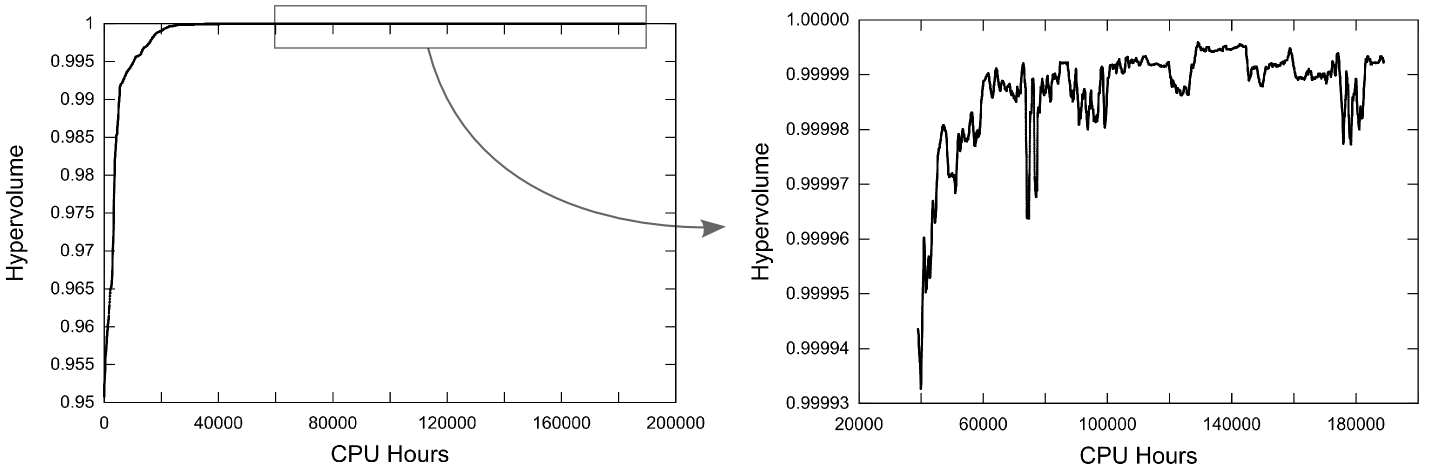
\includegraphics[width=1.0\linewidth]{half_billion_simulation_fig1_hypervolume.png}
  \end{sidecaption}
\end{figure}

After the convergence of the algorithm, $200$ different parameter settings were proposed as possible calibrated sets of parameter values. Because a set of $100$ executions can only provide an approximation of the objective scores of a parameter setting and because we want to make sure that they are well evaluated, $\num{10000}$ more executions of each proposed parameter setting were conducted. After recomputing the dominance selection, the dominated parameter set­ tings were excluded and $62$ parameter settings remained in the Pareto front. As stated above, a multiobjective exploration does not lead to the selection of a single optimized solution but leads to a set of possible candidates for the calibration: each set of parameter settings selected by the procedure represents a specific compromise on the three objectives. Thus, it is possible to distinguish among the parameter settings those satisfying only two objectives out of three from those which offer a better compromise on the three objectives without, however, reaching the best possible values on each objective. This configuration confirms that these three objectives are not redundant and that the procedure vacillates between them to find well-fitted parameter settings. Among the $62$ parameter settings of the Pareto front, some are less satisfying than others. We consider as unsuitable the parameter settings where at least one of the scores of the three objectives has a normalized error over $0.1$ (ie, over $10\%$ of error). Only $29$ parameter settings satisfy this new condition. The values estimated for each parameter of the $29$ selected sets are presented in table \ref{t:parametre}.


The analysis of this new subset shows interesting aspects. First, all of them correctly identify the order of magnitude of the only parameter of the model which can be roughly deduced from the initial conditions and the calibration objectives: the maximum resource parameter ($R_{max}$ ) which is used to limit the logistic growth of the population of each settlement \Anote{foot2}. Second, the four parameters whose values are a priori unpredictable (DistanceDecay, the parameter of dissuasion from the interactions by the distance; $P_{creation}$ , the probability of appearance of an innovation; $P_{diffusion}$ , the probability of its diffusion; and finally InnovationImpact, the impact of the innovation on the growth of the population) are estimated in a very small domain of variation compared with their possible domain of variation (table 3). The ratio between the estimated and theoretical volume defined by these five dimension domains is of \~ $\SI{4.7e-16}{} / \num{320000}{} = \SI{1.5e-21}{}$ ! What is remarkable is how the values taken by each parameter are all in a small neighbourhood, which suggests high reliability considering that they must be given those orders of magnitude to obtain plausible results while using the model for simulation. However it should be noted that the exact values estimated for each parameter do not have any absolute meaning. They only make sense all together, according to their interrelationships in the mechanisms of the model.

\begin{table}[H]
\begin{sidecaption}[fortoc]{Global domain of exploration and calibrated parameter value domain of variation.}[t:domain]
\centering
\begin{tabular}{@{}lll@{}}
\toprule
                   & Explored Domain & Solutions Domain          \\ \midrule
$P_{creation}$     & {[}0,1{]}       & ~{[} \SI{1.1e-06} ; \SI{1.3e-06} {]} \\
$P_{diffusion}$    & {[}0,1{]}       & ~{[} \SI{6.7e-07} ; \SI{6.9e-07} {]} \\
$InnovationImpact$ & {[}0,2{]}       & ~{[} \SI{7.7e-03} ; \SI{8.4e-03} {]} \\
$DistanceDecay$    & {[}0,4{]}       & ~{[} 0.66; 0.75 {]}       \\
$R_{max}$          & {[}1,40000{]}   & ~{[} 10090; 10465 {]}     \\
Volume             & 320000          & ~ \SI{4.7e-16}{}               \\ \bottomrule
\end{tabular}
\end{sidecaption}
\end{table}

Within the subset of $29$ parameter settings there is no way to prefer one setting over the others: the multiple executions of each setting lead to good results and acceptable variability of the outputs. Figures 2 and 3 give an example of such outputs. They depict the results produced by one of the parameter settings (in bold characters \Anote{foot3} in table 2). Figure 2 shows the evolution of the rank–size distribution of settlement sizes during a simulation of the parameter setting. This evolution corresponds to what is expected of the model: a progressive and continuous process of hierarchical organisation of the settlement system (the slope of the linear fit of the rank–size distribution shifts from $0.2$ to $0.9$ in $4000$ years for a maximum reached size reached of about $\num{10000}$ inhabitants). This result is quite robust if we consider the low variability of the recorded final state from one simulation to another (figure 3).


\begin{table}[!htbp]
\begin{sidecaption}[fortoc]{Calibrated parameter settings (rounded values).}[t:calibrated]
\resizebox{\columnwidth}{!}{%
\begin{tabular}{@{}llllllll@{}}
\multicolumn{5}{l}{Parameter setting}                                               & \multicolumn{3}{l}{\% error for each objective score}                                                                                                                                           \\ \midrule
$R_{max}$ & \begin{tabular}[c]{@{}l@{}}$Distance$ \\ $Decay$ \end{tabular}  & $P_{creation}$ & $P_{diffusion}$ &  \begin{tabular}[c]{@{}l@{}}$Innovation$ \\ $Impact$ \end{tabular} & \begin{tabular}[c]{@{}l@{}}distribution \\ objective\end{tabular} & \begin{tabular}[c]{@{}l@{}}population \\ objective\end{tabular} & \begin{tabular}[c]{@{}l@{}}time \\ objective\end{tabular} \\ \midrule
$\num{10464}$     & $\num{0.691}$           & \SI{1.11e-06}{}       & \SI{7.90e-07}{}        & $\num{0.0077}$                        & $\num{2.02}$                                                 & $\num{6.59}$                                                            & $\num{1.00}$                                                      \\
$\num{10465}$     & $\num{0.709}$           & \SI{1.14e-06}{}       & \SI{7.88e-07}{}        & $\num{0.0078}$                        & $\num{2.04}$                                                 & $\num{7.31}$                                                            & $\num{0.10}$                                                      \\
$\num{10459}$     & $\num{0.705}$           & \SI{1.15e-06}{}       & \SI{7.92e-07}{}        & $\num{0.0077}$                        & $\num{2.22}$                                                 & $\num{6.98}$                                                            & $\num{0.48}$                                                      \\
$\num{10465}$     & $\num{0.708}$           & \SI{1.15e-06}{}       & \SI{7.86e-07}{}        & $\num{0.0078}$                        & $\num{2.51}$                                                 & $\num{6.00}$                                                            & $\num{0.40}$                                                      \\
$\num{10261}$     & $\num{0.679}$           & \SI{1.17e-06}{}       & \SI{7.78e-07}{}        & $\num{0.0078}$                        & $\num{2.79}$                                                 & $\num{5.29}$                                                            & $\num{4.55}$                                                      \\
$\num{10262}$     & $\num{0.679}$           & \SI{1.15e-06}{}       & \SI{7.52e-07}{}        & $\num{0.0078}$                        & $\num{2.95}$                                                 & $\num{5.00}$                                                            & $\num{2.15}$                                                      \\
$\num{10262}$     & $\num{0.665}$           & \SI{1.14e-06}{}       & \SI{7.24e-07}{}        & $\num{0.0078}$                        & $\num{2.99}$                                                 & $\num{5.53}$                                                            & $\num{1.23}$                                                      \\
$\num{10261}$     & $\num{0.683}$           & \SI{1.12e-06}{}       & \SI{7.38e-07}{}        & $\num{0.0080}$                        & $\num{3.1 }$                                                 & $\num{4.34}$                                                            & $\num{1.15}$                                                      \\
$\num{10260}$     & $\num{0.699}$           & \SI{1.17e-06}{}       & \SI{7.38e-07}{}        & $\num{0.0079}$                        & $\num{3.62}$                                                 & $\num{5.51}$                                                            & $\num{0.20}$                                                      \\
$\num{10287}$     & $\num{0.690}$           & \SI{1.23e-06}{}       & \SI{7.56e-07}{}        & $\num{0.0078}$                        & $\num{3.63}$                                                 & $\num{3.74}$                                                            & $\num{3.46}$                                                      \\
$\mathbf{\num{10259}}$     & $\mathbf{\num{0.688}}$           & $\mathbf{\SI{1.20e-06}{}}$       & $\mathbf{\SI{7.41e-07}{}}$        & $\mathbf{\num{0.0079}}$                        & $\mathbf{\num{3.74}}$                                                 & $\mathbf{\num{3.55}}$                                                            & $\mathbf{\num{2.48}}$                                                      \\
$\num{10169}$     & $\num{0.736}$           & \SI{1.29e-06}{}       & \SI{7.39e-07}{}        & $\num{0.0079}$                        & $\num{4.90}$                                                 & $\num{5.20}$                                                            & $\num{0.03}$                                                      \\
$\num{10205}$     & $\num{0.683}$           & \SI{1.19e-06}{}       & \SI{7.42e-07}{}        & $\num{0.0082}$                        & $\num{5.10}$                                                 & $\num{2.60}$                                                            & $\num{6.03}$                                                      \\
$\num{10126}$     & $\num{0.738}$           & \SI{1.22e-06}{}       & \SI{7.61e-07}{}        & $\num{0.0082}$                        & $\num{5.69}$                                                 & $\num{2.88}$                                                            & $\num{1.50}$                                                      \\
$\num{10126}$     & $\num{0.738}$           & \SI{1.24e-06}{}       & \SI{7.39e-07}{}        & $\num{0.0082}$                        & $\num{6.02}$                                                 & $\num{3.08}$                                                            & $\num{0.55}$                                                      \\
$\num{10096}$     & $\num{0.701}$           & \SI{1.14e-06}{}       & \SI{7.14e-07}{}        & $\num{0.0084}$                        & $\num{6.12}$                                                 & $\num{2.58}$                                                            & $\num{1.55}$                                                      \\
$\num{10169}$     & $\num{0.736}$           & \SI{1.29e-06}{}       & \SI{7.39e-07}{}        & $\num{0.0080}$                        & $\num{6.25}$                                                 & $\num{2.46}$                                                            & $\num{1.20}$                                                      \\
$\num{10165}$     & $\num{0.734}$           & \SI{1.29e-06}{}       & \SI{7.24e-07}{}        & $\num{0.0080}$                        & $\num{6.31}$                                                 & $\num{2.91}$                                                            & $\num{0.30}$                                                      \\
$\num{10121}$     & $\num{0.732}$           & \SI{1.28e-06}{}       & \SI{7.41e-07}{}        & $\num{0.0081}$                        & $\num{6.41}$                                                 & $\num{2.36}$                                                            & $\num{1.90}$                                                      \\
$\num{10164}$     & $\num{0.735}$           & \SI{1.29e-06}{}       & \SI{7.27e-07}{}        & $\num{0.0080}$                        & $\num{6.45}$                                                 & $\num{2.74}$                                                            & $\num{0.45}$                                                      \\
$\num{10103}$     & $\num{0.733}$           & \SI{1.24e-06}{}       & \SI{7.42e-07}{}        & $\num{0.0084}$                        & $\num{7.67}$                                                 & $\num{1.90}$                                                            & $\num{3.10}$                                                      \\
$\num{10092}$     & $\num{0.736}$           & \SI{1.29e-06}{}       & \SI{7.14e-07}{}        & $\num{0.0082}$                        & $\num{7.81}$                                                 & $\num{2.22}$                                                            & $\num{1.10}$                                                      \\
$\num{10098}$     & $\num{0.737}$           & \SI{1.29e-06}{}       & \SI{7.12e-07}{}        & $\num{0.0082}$                        & $\num{7.84}$                                                 & $\num{2.55}$                                                            & $\num{0.58}$                                                      \\
$\num{10094}$     & $\num{0.741}$           & \SI{1.28e-06}{}       & \SI{7.12e-07}{}        & $\num{0.0083}$                        & $\num{8.46}$                                                 & $\num{1.99}$                                                            & $\num{1.00}$                                                      \\
$\num{10129}$     & $\num{0.737}$           & \SI{1.29e-06}{}       & \SI{7.07e-07}{}        & $\num{0.0082}$                        & $\num{8.64}$                                                 & $\num{1.97}$                                                            & $\num{0.68}$                                                      \\
$\num{10110}$     & $\num{0.735}$           & \SI{1.28e-06}{}       & \SI{6.77e-07}{}        & $\num{0.0083}$                        & $\num{9.04}$                                                 & $\num{2.48}$                                                            & $\num{0.03}$                                                      \\
$\num{10091}$     & $\num{0.744}$           & \SI{1.31e-06}{}       & \SI{7.25e-07}{}        & $\num{0.0083}$                        & $\num{9.22}$                                                 & $\num{1.51}$                                                            & $\num{2.68}$                                                      \\
$\num{10091}$     & $\num{0.741}$           & \SI{1.31e-06}{}       & \SI{7.12e-07}{}        & $\num{0.0083}$                        & $\num{9.61}$                                                 & $\num{1.49}$                                                            & $\num{2.15}$                                                      \\
$\num{10109}$     & $\num{0.734}$           & \SI{1.28e-06}{}       & \SI{6.79e-07}{}        & $\num{0.0084}$                        & $\num{9.64}$                                                 & $\num{1.77}$                                                            & $\num{0.18}$                                                      \\ \bottomrule
\end{tabular}%
}
\end{sidecaption}
\end{table}

\begin{figure}[!htbp]
\begin{sidecaption}[fortoc]{Evolution of the rank–size distribution during a simulation of one of the best calibrated parameter settings.}[fig:S_ranksize]
  \centering
 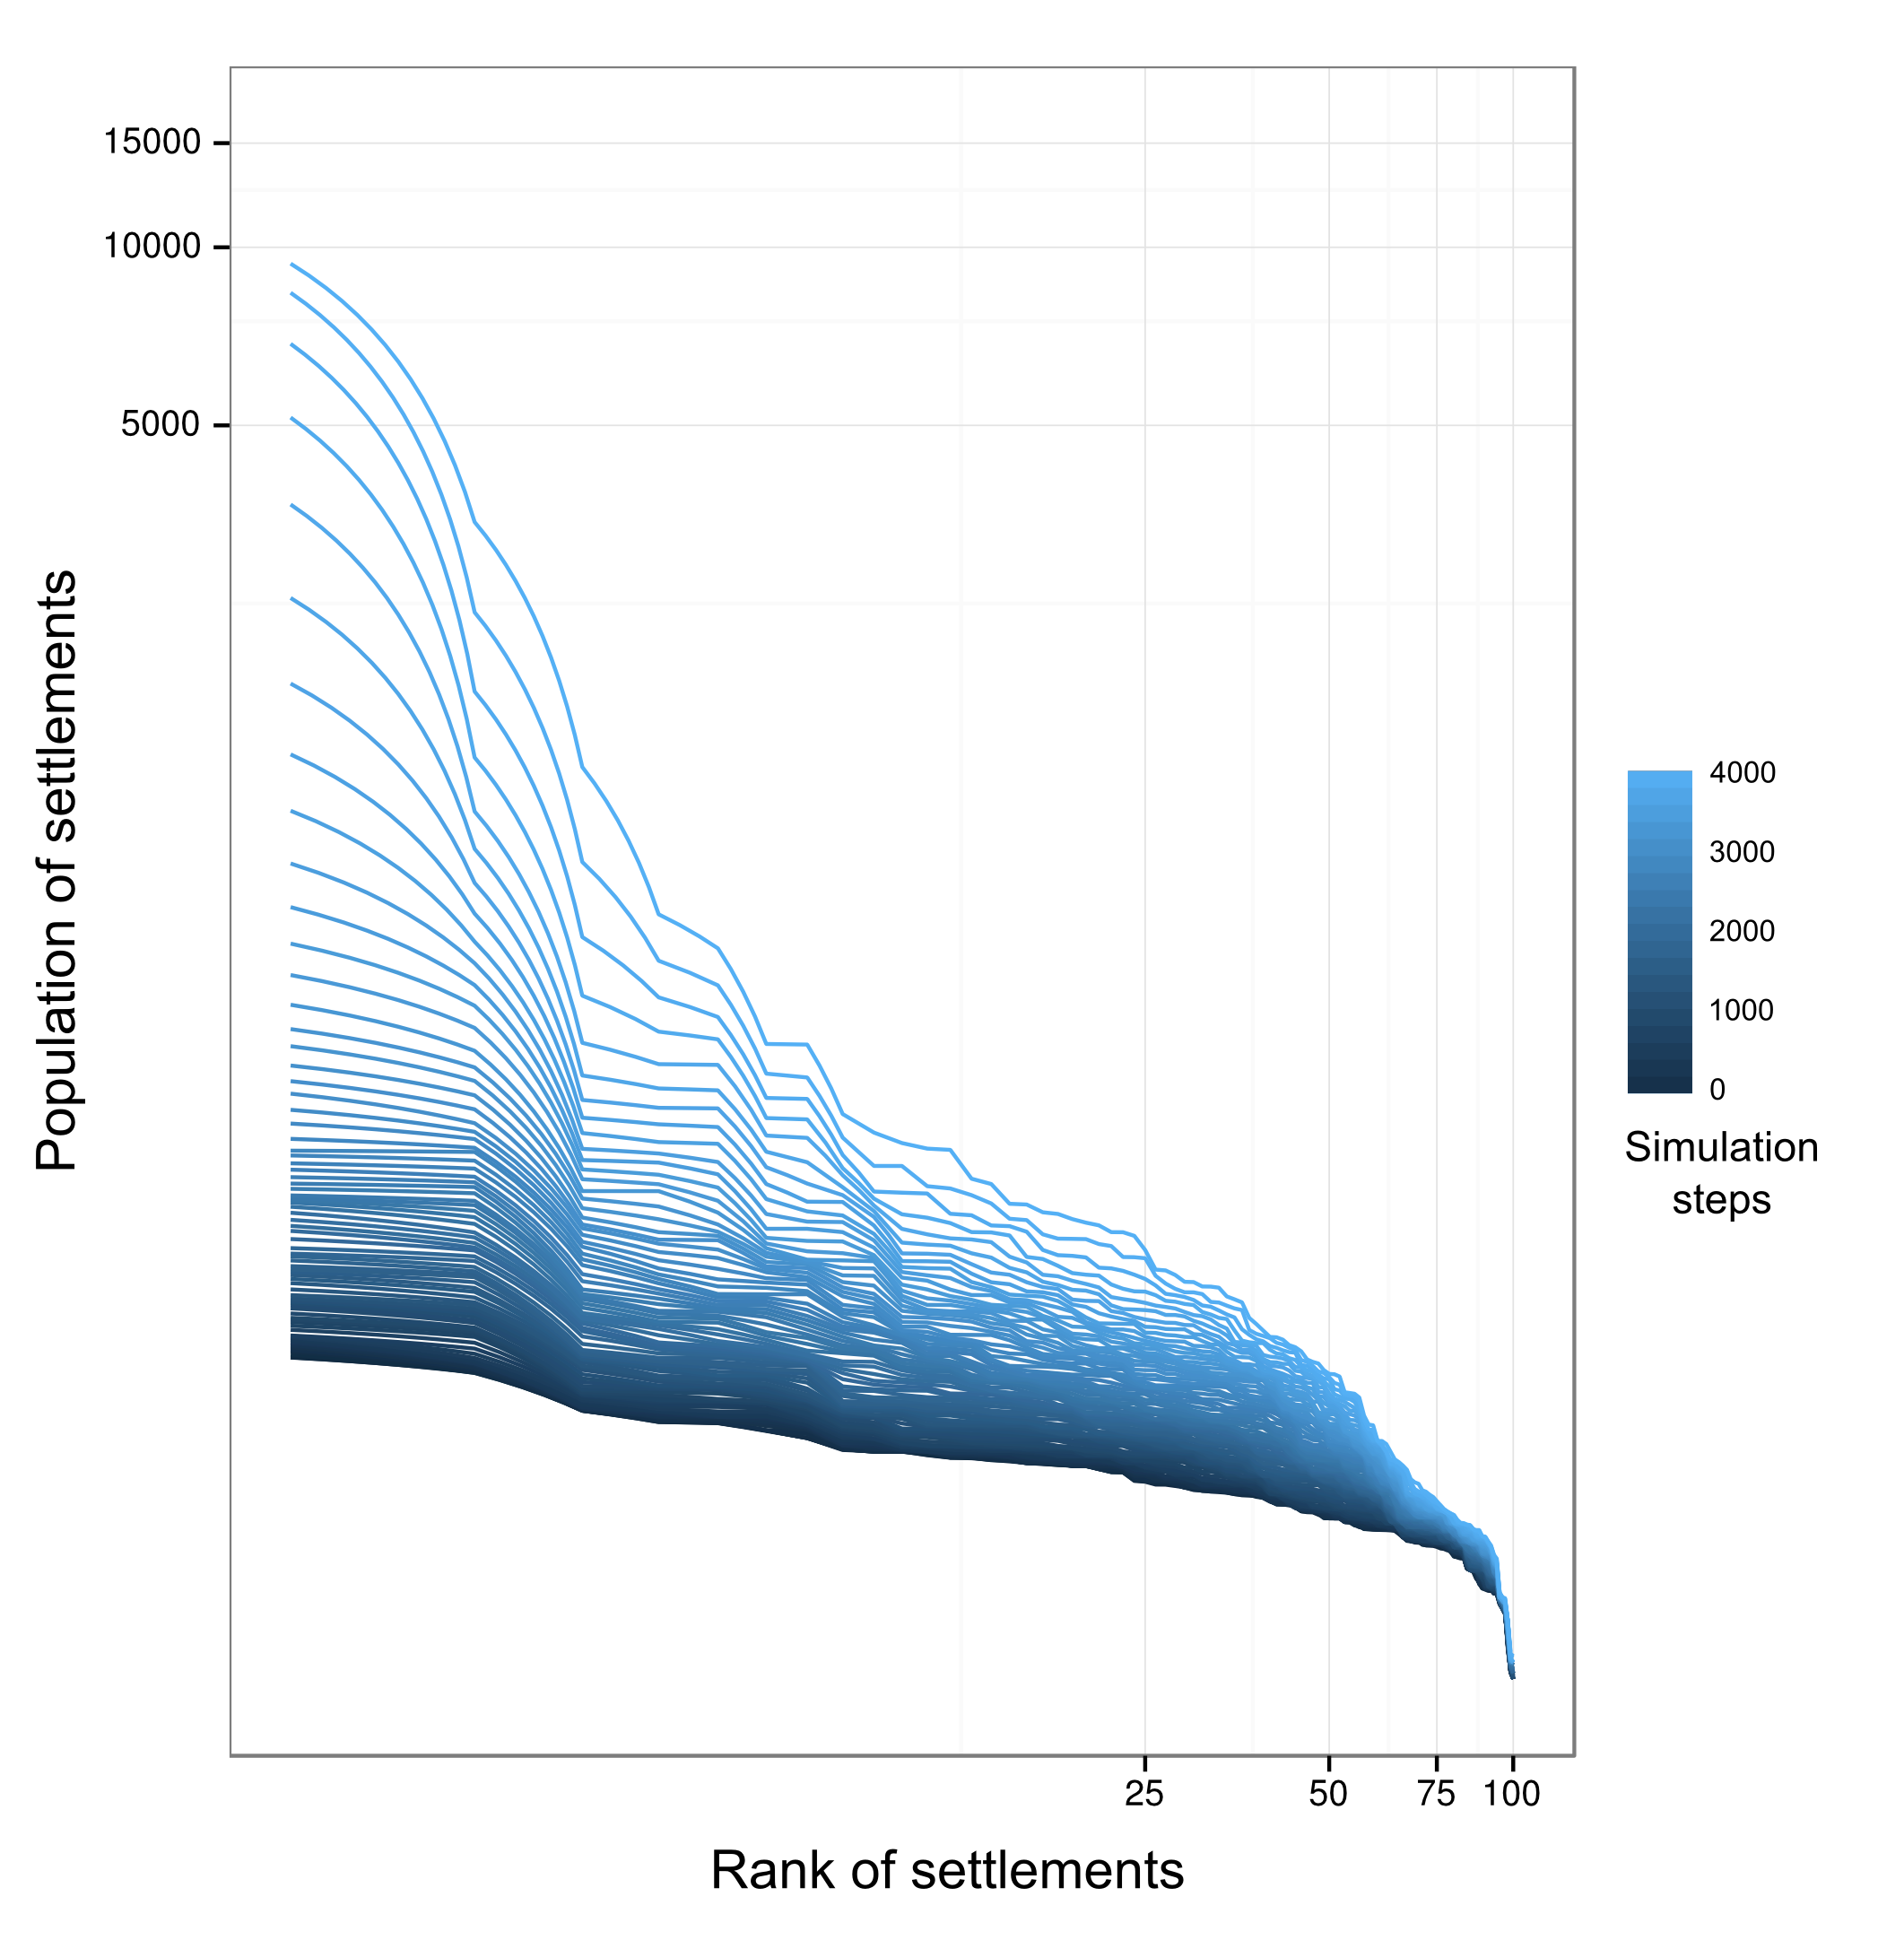
\includegraphics[width=1.0\linewidth]{RTbleu.png}
  \end{sidecaption}
\end{figure}

\begin{figure}[!htbp]
\begin{sidecaption}[fortoc]{Variability of the rank–size distribution at the final simulation step in 100 simulations of one of the best calibrated parameter settings.}[fig:S_hypervolumemedian]
  \centering
 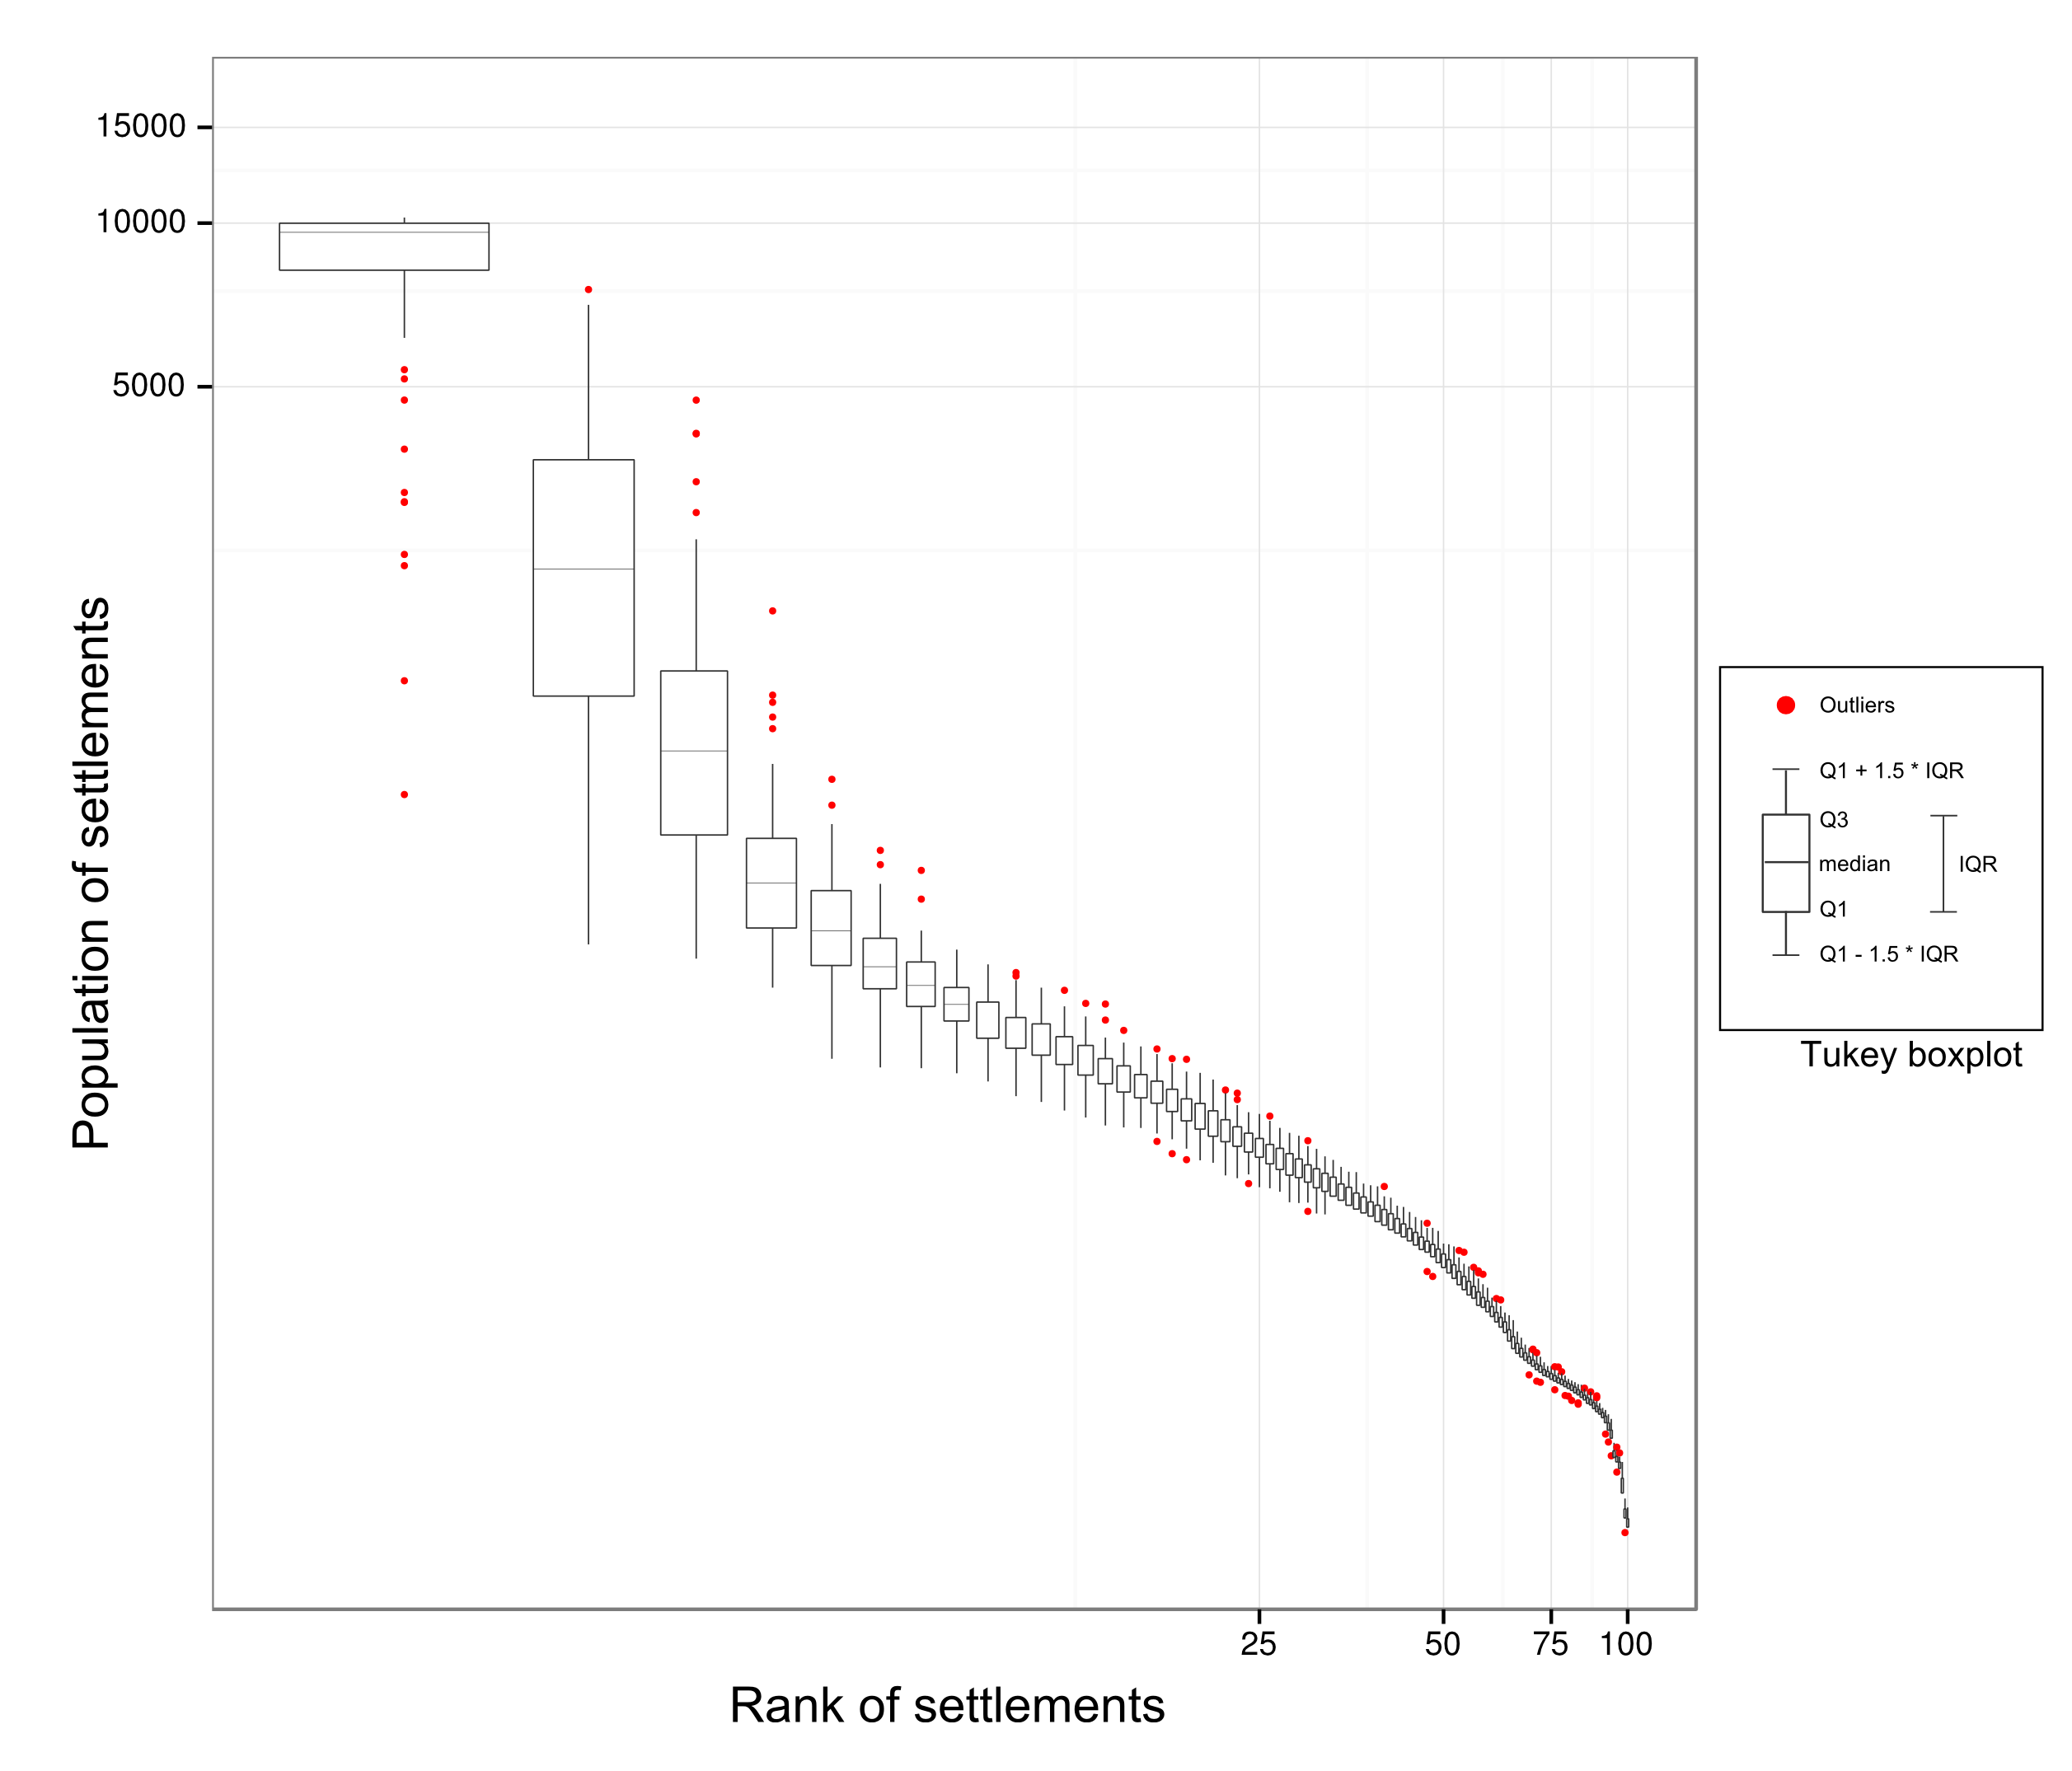
\includegraphics[width=1.0\linewidth]{varRTrouge.png}
  \end{sidecaption}
\end{figure}

\section{Conclusion}
\label{sec:conlusion}

An automatic calibration procedure was applied for the first time on a multiagent model, SimpopLocal, which was developed to simulate the emergence of a system of urban settlements. It provides convincing results to solve the calibration problem for multiagent models. With five parameters whose value could not be estimated from empirical data, it would have been quite difficult to find an estimation of a calibrated parameter setting ‘manually’. By reversing this calibration problem into an optimisation problem, our automated calibration procedure generates parameter settings which reproduce the stylized facts embodied in three objective functions very well. This enables us to confirm a decisive advance in the validation of this model: we proved that the SimpopLocal model, as conceived in its simplicity, is able to satisfactorily generate a plausible evolution including the emergence of an urban hierarchy. and quantifying criteria for evaluating the model; a methodology for exploring the parameter space with an automated process using evolutionary algorithms; a technical protocol for reducing the exploration time by massive distributed computing. The application of these principles to modelling not only improves the quality of communication about the model, but also ensures the repeatability of its experimentation and contributes to creating accessible modelling tools that can be shared via the free and open-source software tool for model experiments. OpenMOLE ( \href{http://www.openmole.org}{http://www.openmole.org}) . In order to help the dissemination of these techniques, we published several tutorials on the developed tools. For example, on how to design a grid exploration of a NetLogo model \Anote{foot4} and how to explore a NetLogo model with evolutionary algorithms. \Anote{foot5} This work forges a path for other modellers, who could use a similar data-intensive grid-based approach in their modelling experiments.

\textbf{Acknowledgments.} This work is funded by the ERC Advanced Grant Geodivercity, the Agence de l’Environnement et la Maitrise de l’Energie, the network Réseau de Recherche sur le Développement Soutenable, and the Institut des Systèmes Complexes Paris Île-de-France. Results obtained in this paper were computed on the biomed and the vo.complex-system.eu virtual organization of the European Grid Infrastructure ( http://www.egi.eu ). We thank the European Grid Infrastructure and its supporting National Grid Initiatives (France-Grilles in particular) for providing the technical support and infrastructure. We also thank an anonymous reviewer for help in improving the first version of the paper.

\section{Annexe}
\label{sec:annexe}

\begin{figure}[!htbp]
\begin{sidecaption}[fortoc]{Diagramme de classe}[fig:S_classe]
  \centering
 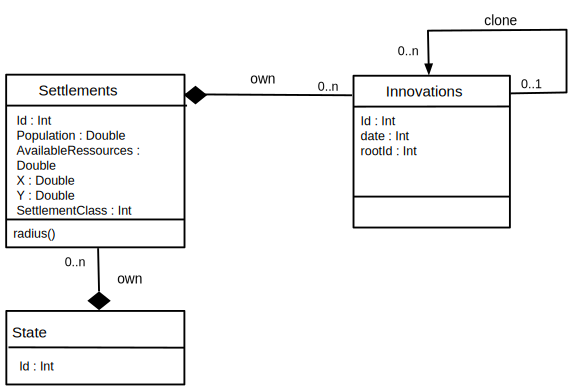
\includegraphics[width=1.0\linewidth]{slocal_uml.pdf}
  \end{sidecaption}
\end{figure}

\begin{figure}[!htbp]
\begin{sidecaption}[fortoc]{Diagramme d'activité principal}[fig:S_activite]
  \centering
 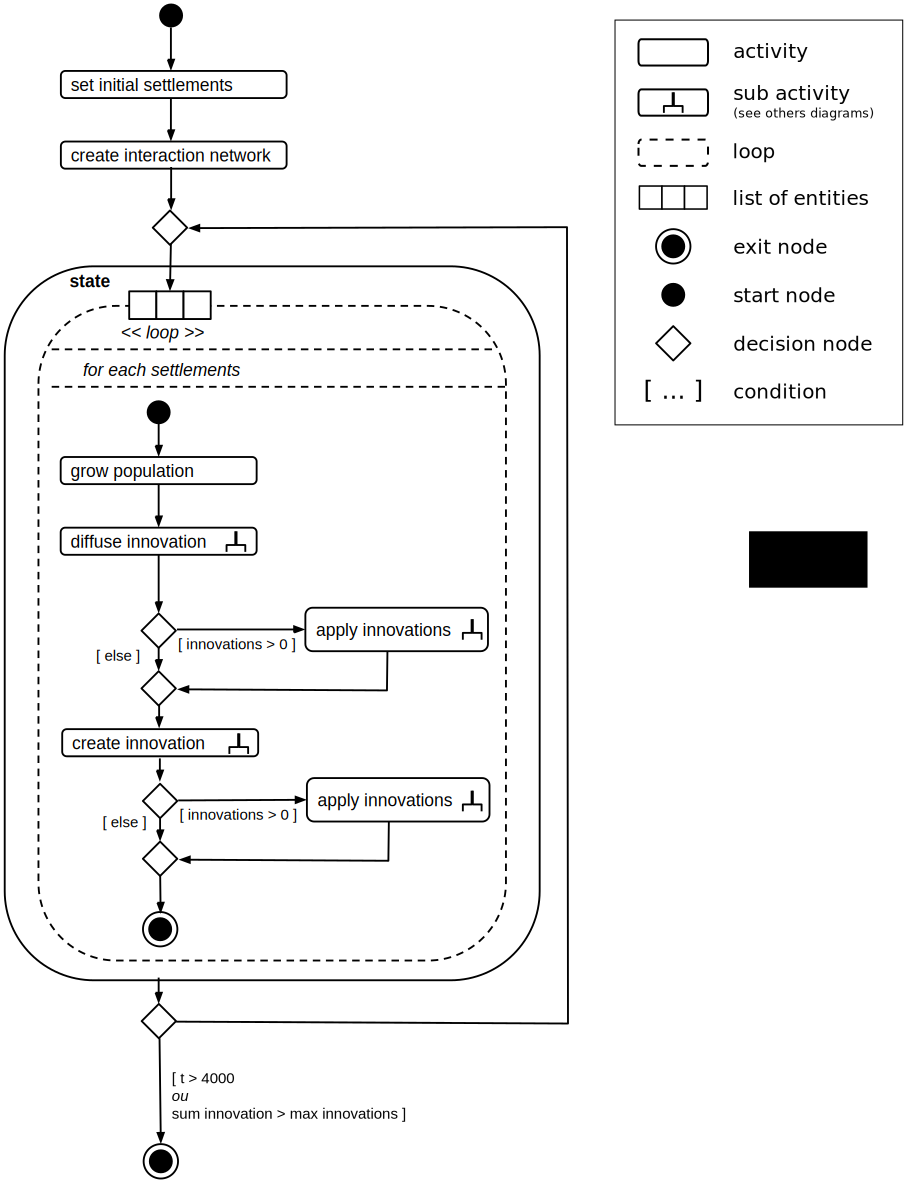
\includegraphics[width=0.9\linewidth]{slocal_state.pdf}
  \end{sidecaption}
\end{figure}

\begin{figure}[!htbp]
\begin{sidecaption}[fortoc]{Diagramme d'activité pour la gestion des innovations}[fig:S_activite]
  \centering
 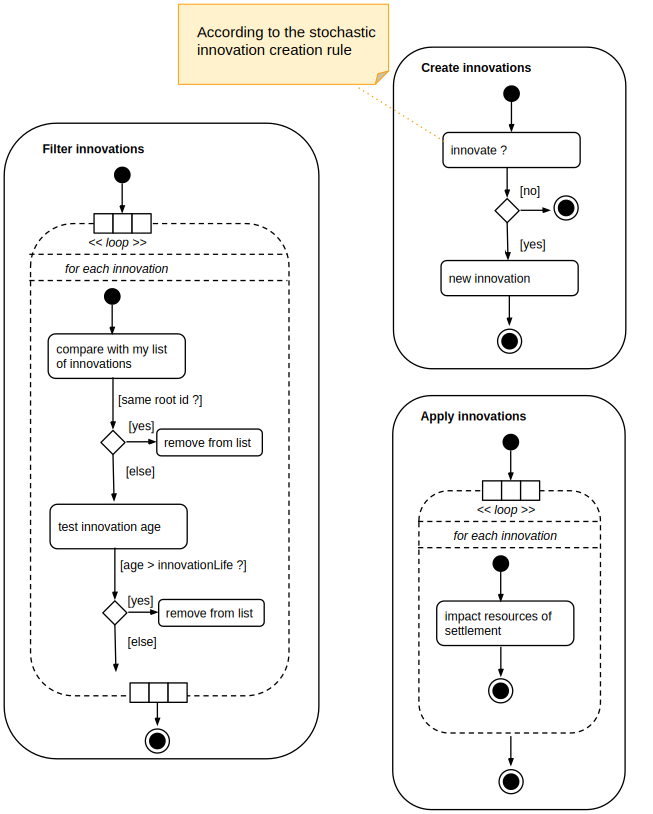
\includegraphics[width=1.0\linewidth]{slocal_groupeinov.pdf}
  \end{sidecaption}
\end{figure}

\begin{figure}[!htbp]
\begin{sidecaption}[fortoc]{Diagramme d'activité pour la gestion des innovations}[fig:S_activite]
  \centering
 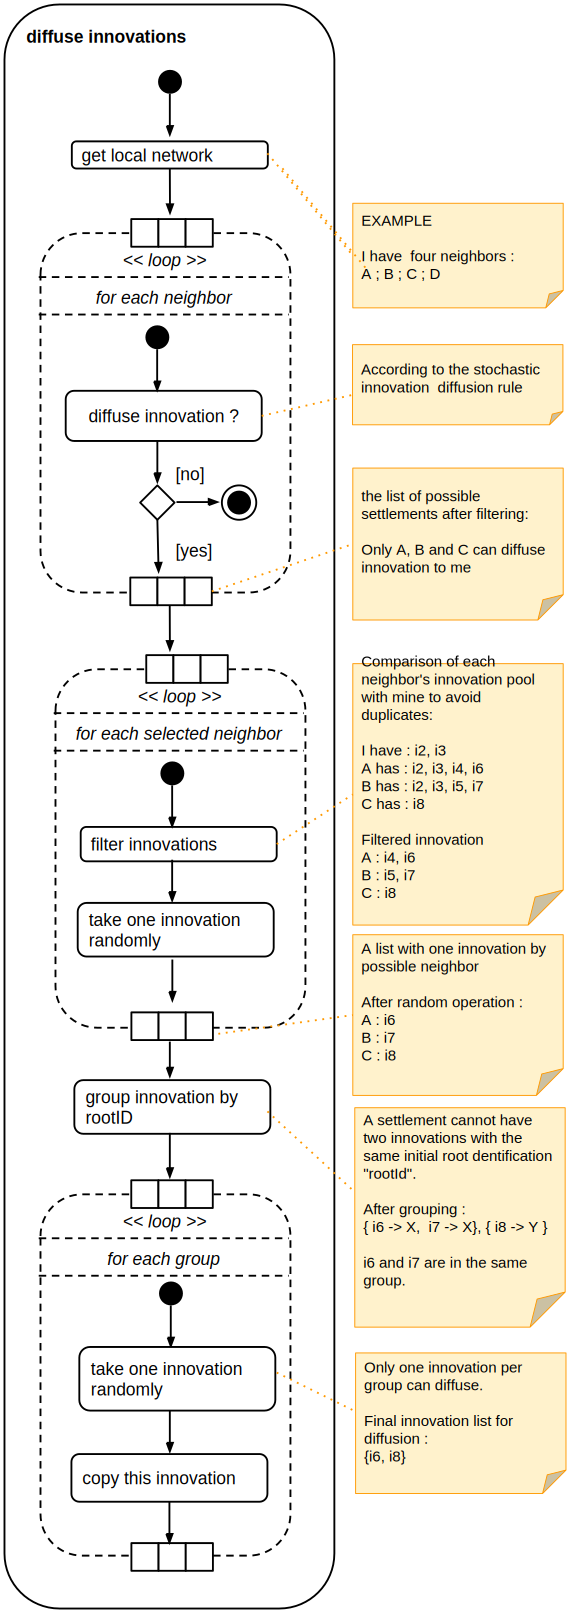
\includegraphics[width=1.0\linewidth]{slocal_diffuse.pdf}
  \end{sidecaption}
\end{figure}

\printbibliography[heading=subbibliography]


% -*- root: These.tex -*-

%%ENTRETIENT
\chapter{Entretiens}
\label{chap:entretiens}

\section{Entretien avec le professeur historien et médiéviste Jean-Philippe Genet}
\label{sec:entretient_genet}

\noindent\textbf{- Entretien réalisé le : } 13 mai 2015 \\
\noindent\textbf{- Transcription faite le :} 14 mai 2015 \\
\noindent\textbf{- Validation faite le :} en attente de confirmation, la version définitive apparaitra dans quelques semaines dans la version de la thèse déposée sur Internet.

\paragraph*{Sébastien Rey : Si vous pouviez m'en dire plus sur le type de matériel, l'ouverture du centre ?}

\noindent\emph{Jean-Philippe Genet}: Le centre je ne l'ai connu que quand je suis revenu ici. J'ai été assistant à la Sorbonne en 1967, et à l'époque il n'y avait pas encore Paris 1, c'était la Sorbonne, tout était donc ensemble. Je n'ai pas entendu de suite parler d'informatique, en tout cas chez les historiens. Il y avait bien des historiens qui en faisaient à cette époque, mais ils n'en faisaient pas ici, ou alors dans des endroits relativement, disons, je dirais occultes. A ma connaissance, les deux personnes qui s'intéressaient à l'informatique à l'époque, donc en 1967, c'était surtout \textbf{Antoine Prost}, qui travaillait dans le centre d'histoire contemporaine, qui à l'époque réunissait le dix-neuvième et le vingtième siècle. Il y avait aussi, quelqu'un, je pense qu'il était déjà là, je n'en suis pas absolument sûr, qui s'appelait \textbf{William Serman}. Et donc il faisait de l'analyse de discours, avec un informaticien qui s'appelait \textbf{Édouard Cadet}, un Haïtien, un type très bien, je l'ai un peu fréquenté. Je savais que cela existait, mais on ne pouvait pas être au courant si on n’appartenait pas spécifiquement à ce centre-là, il n'y avait pas d'activité en cours.
Donc ensuite j'ai fait mon service militaire complet à Paris 1, c'était en douce, et après je suis parti à Oxford pendant un an. Quand je suis rentré, je me suis mis sérieusement à l'informatique, j'ai donc pris des cours et çà je l'ai fait à Paris 5. J'ai suivi les cours de \textbf{Marc Barbut}, et puis des gens qui étaient dans son équipe. J'ai ensuite commencé à me préoccuper pour en faire  dans le cadre de mes recherches. A ce moment-là, je n'avais pas vraiment entendu parler du centre de calcul de Paris 1, et c'est seulement à l'automne 70 que je me suis vraiment préoccupé de faire quelque chose. Alors, ce que j'ai trouvé à ce moment-là durant l'année 70-71, c'est un ordinateur qui a été remplacé très rapidement, un IBM classique assez poussif. Il a été remplacé rapidement par une machine qui était un  Philips P880.

\paragraph*{Sébastien Rey : Ce numéro vous a marqué en tout cas.}

\noindent\emph{Jean-Philippe Genet}: Oui, car celui-là on a beaucoup travaillé dessus. On avait deux types d'activités : de la prosopographie (analyse de biographie avec des méthodes statistiques y compris l'analyse factorielle) faite sur le P880, et puis je faisais de l'analyse lexicale sur les grosses machines d'Orsay sur des crédits des CNRS, sur lesquelles on pouvait passer la nuit, ou le samedi et le dimanche. J'avais une Diane à l'époque, que je chargeais de bac de cartes perforées, je les trainais sur le sol, et puis on allait passer le samedi jusqu'à ce que mort s'ensuive à Orsay. On travaillait en mode batch, vous lancez l'exécution et vous attendez le retour, qui est une erreur en général. Une virgule qui manque quelque part, vous cherchez la faute, vous la corrigez, et puis vous relancez jusqu'à ce que ça finisse par passer. La grande différence par rapport à ce qu'on faisait en local, c'est que pour travailler à Orsay, il fallait des crédits CNRS.

\paragraph*{Sébastien Rey : Cela coûtait cher pour l'époque ?}

\noindent\emph{Jean-Philippe Genet}: Ce n’est pas que c'était très cher, mais il fallait surtout demander au comité national du CNRS l'autorisation, et obtenir un crédit, faire un dossier, etc. bref c'était compliqué. Donc je l'ai fait, j'ai obtenu un crédit, je m'en souviens très bien, mon premier crédit était de mille francs, et je recevais un carnet de chèques. C'était très bien d'ailleurs, la gestion n'était pas très compliquée, mais ça marchait très bien. Ceci dit cela ne servait à rien dans le cas d'Orsay, puisque là c'était des virements internes, donc je n’ai jamais touché au carnet de chèques. Avec ce travail à Orsay on est monté en puissance, on est devenu une vraie équipe CNRS,  puis un laboratoire du CNRS (date?). Tout cela a pris beaucoup d'importance et bientôt on n'était plus obligé d'aller à Orsay, et on a pu travailler au Laboratoire Informatique des Sciences de l'Homme.

\paragraph*{Sébastien Rey : Donc à la MSH, au LISH}

\noindent\emph{Jean-Philippe Genet}:Voilà, à la MSH, boulevard Raspail, c'est là que j'ai connu Philippe Cibois.

\paragraph*{Sébastien Rey : À quelle date environ ? }

\noindent\emph{Jean-Philippe Genet}: Cela doit être dans les années 75-80, franchement je suis très mauvais sur les dates, je suis médiéviste alors tout ça ... je vois plus loin :)

Par contre pour tout le travail, disons sur les bases de données, on travaillait sur le Philips P880, et c'est là où il y avait un club d'utilisateur assez restreint. En économie il y avait Pierre-Yves Hénin, et une personne qui s'appelait \textbf{Pouchain} qui était un économiste qui travaillait avec \textbf{Hénin}. Il y avait les trois géographes \textbf{Thérése Saint Julien}, \textbf{Denise Pumain}, et puis un spécialiste de la France qui s'appelait \textbf{Yvan Chauviré} je crois. Il est resté à Paris 1 assez longtemps, mais il n'y est plus maintenant.


\paragraph*{Sébastien Rey : Ça donc, c'était l'équipe de base ?}

\noindent\emph{Jean-Philippe Genet}: Oui l'équipe de base, et puis il y avait d'autres utilisateurs, bien sûr, mais le fonctionnement était assez bon grâce à cette équipe. Il y avait le dieu tutélaire qu'on ne voyait jamais qui passait de temps en temps, un économiste, qui était vital, car c'était de lui que dépendait le centre, et puis comme il était très respecté chez les économistes ... il s'appelait \textbf{Claude Fourgeaud}. Celui-ci était un professeur d'économie déjà âgé, qui avait déjà eu une attaque, un peu bizarre comme ça, mais c'était un universitaire, semble-t-il très fort et en tout cas très respecté. Ce qui fait que le centre de calcul a toujours eu les moyens qu'il lui fallait. La tête pensante pour les machines, les ingénieurs, etc. c'était \textbf{Édouard Valensy}. Celui-ci enseignait à Paris 1, mais c'était un général polytechnicien, qui s'occupait du centre de recherche de l'armée à Saclay, et qui avait donc cette grande qualité de nous fournir en informaticiens quand on voulait travailler sur des projets scientifiques, des gens d'une très très grande qualité intellectuelle. Pour éviter le problème d'aller à Orsay, j'ai pu développer justement mon logiciel d'analyse lexicale avec deux garçons : \textbf{Jacques Mondelli} qui est devenu un cadre très important chez Bull, et qui est mort malheureusement de la maladie de l'amiante, car les centres de calcul à l'époque n'étaient pas non plus des endroits très sains. Et François Hucher qui a travaillé par la suite à la C2I. L'un était de l'école des mines Berkeley, et l'autre était Centralien. Donc évidemment c'était des gens qui étaient à la pointe du combat en informatique, et on a pu faire vraiment à ce moment-là du bon travail. Bien qu'ayant des moyens dérisoires. Le centre de calcul lui-même c'était toujours le P880, ici à Paris 1. Celui qui le faisait tourner pour nous surtout, c'était un gars qui s'appelait \textbf{Xavier Debanne}. Je crois qu'il est devenu catholique convaincu, il est parti à Rome en tout cas et il a fondé plus ou moins une boîte, et il a travaillé plus ou moins avec le Vatican. Il travaillait à cette époque avec \textbf{Jean-Paul Trystram}, quelqu'un qui était un prof un peu inclassable, ayant également fait un manuel d'informatique pour les sciences sociales. \textbf{Xavier Debanne} avait développé pour un logiciel qui s'appelait BDP2 (banque de données paris 1 version 2), devenu ensuite BDP3, jusqu'à BDP4, et qui marchait très bien. En gros c'était un SPSS miniature, mais qui vous permettez de faire tous les tests, tout çà sur cartes perforées. On faisait ça avec le P880, car il tolérait d'assez gros fichiers, donc on pouvait traiter des bases de données importantes, faire des tris croisés, des analyses factorielles, et tout ça c'était quand même pas mal. 

Le centre de calcul était organisé ainsi, il y avait la salle avec l'ordinateur, et à côté il y avait une petite salle où les dames  faisaient les perforations. Il y avait deux perforeuses, et puis nous, enfin tous les chercheurs, on se faisait les perforations nous-mêmes la plupart du temps. 

\paragraph*{Sébastien Rey : Denise m'a également parlé de ces deux dames.}

\noindent\emph{Jean-Philippe Genet}: C'était les piliers de la maison, elles avaient leur franc-parler, et c'était assez pittoresque, surtout une. Et elles ne s'envoyaient pas dire quand quelqu'un faisait une erreur, cela fusait. 
 
\paragraph*{Sébastien Rey : Donc celles-ci étaient employées à plein temps.}

\noindent\emph{Jean-Philippe Genet}: Oui elles faisaient des petits trous toute la journée, avec une vitesse évidemment qu'enviaient beaucoup les malheureux qui faisaient leurs cartes perforées eux-mêmes.

\paragraph*{Sébastien Rey : Vous savez jusqu'à quand ça a duré ?}

\noindent\emph{Jean-Philippe Genet}: Tout ça a duré assez longtemps, car le CNRS a beaucoup renâclé à pousser la micro-informatique. C'est çà un des problèmes, d'ailleurs Cibois vous en a peut-être parlé.

\paragraph*{Sébastien Rey : Oui c'est arrivé vers les années 1980 - 1984, plutôt sur initiative de quelques personnes.}

\noindent\emph{Jean-Philippe Genet}: C'était beaucoup dans le cadre du CRH (centre de recherche historique). Enfin, il y avait certaines personnes qui connaissaient les universités américaines, et qui dès lors qu'elles sont revenues en France ont dit à ce moment-là \enquote{ça ne va pas} . Moi de mon point de vue, je n'étais même pas au courant. J'ai découvert ça presque un peu tard. Ici à Paris 1 on n’avait pas de micro-ordinateur, on travaillait toujours sur le P880, et surtout on n’avait pas les logiciels, donc on continuait à travailler avec le logiciel BDP4 qui fonctionnait bien. J'avais mon système qui s'appelait ALINE pour l'analyse linguistique qui fonctionnait également bien, donc je n'allais pas changer pour des micro-ordinateurs pour lequel il n'y avait aucun logiciel. D'ailleurs le CNRS ne nous y encourageait pas, il ne voulait pas nous donner d'argent pour qu'on achète des micro-ordinateurs, c'était explicite. Et parce que'il voulait surtout continuer à nous faire financer. En fait il donnait aux équipes des sciences humaines des crédits, pour faire de l'informatique, mais ces crédits étaient ensuite convertis automatiquement en crédits reversés au centre de calcul du CIRCE à Orsay. En fait l'argent ne faisait qu'un détour par nous, il tournait en rond et revenait dans leur système. Donc il ne nous poussait pas du tout à faire de la micro-informatique. Sans compter qu'évidemment on est toujours méfiant, dès que le fonctionnaire va se trouver autonome, il va regarder YouTube, enfin à l'époque ça n’existait pas. À l'époque le truc le plus « in », c'était vous savez les balles de tennis qui rebondissent, pong ... Donc il fallait que l'on continue à travailler avec les grosses machines.

Tout çà a quand même eu une fin. De toute façon j'avais déjà commencé à faire de l'enseignement de l'informatique pour les historiens à Paris 1. J'ai dû commencer dans les années 1977-78 quand les deux logiciels commençaient à bien tourner. La difficulté c'est que comme on n’avait pas de micro-ordinateur, on allait en procession rue cujas jusqu'au bâtiment de la fac de droit pour faire du batch sur le Philips P880.

\paragraph*{Sébastien Rey : Le Philipps était situé où dans le bâtiment ?}

\noindent\emph{Jean-Philippe Genet}: Quand vous rentrez au panthéon, vous voyez la cour, vous allez au coin droit, vous rentrez dans le bâtiment, et c'était là juste à droite. Au pied du grand escalier qui monte, c'était là, les trois-quatre pièces qui étaient là. Ce n’était pas grand.
Il y avait d'autres gens qui faisaient de l'informatique à Paris 1, par exemple \textbf{Colette Roland}, mais elle ne s'est jamais intéressée à ça, je ne l'ai jamais vu travailler sur une machine du centre. Elle faisait plus de la théorie informatique. La seule personne qui vraiment a été l'âme du centre, et qui l'a fait fonctionner, c'était \textbf{Yvonne Girard}, une mathématicienne. C'est elle qui a assuré le fonctionnement du centre pendant de longues années.

Je ne me souviens plus de l'année exacte 1984-85, mais  il y a \textbf{Jean-Pierre Bardet}, un historien démographe de Paris 4, qui a été ensuite au ministère de la Recherche. Un jour il en a eu marre de tout ça, car à Paris 4 c'était pire, nous on avait un centre de calcul, mais eux il en avait à peine. \textbf{Jean-Pierre Bardet} travaillait beaucoup au LISH, et je travaillais avec lui. On lui avait même prêté nos machines pour imprimer sa thèse, car la sienne était tombée en panne la veille de la soutenance, le type d'événement qui crée des liens. Et quand il s'est trouvé au ministère, \textbf{Jean-Pierre Bardet} a changé tout ça. Il a envoyé aux départements d'histoire, un petit peu partout en France, des micro-ordinateurs. C'était des Bull 45, à l'époque c'était bien, c'était des PC de base si vous voulez. Et il en a envoyé 12 à Paris 1 à l'UFR d'histoire. Le directeur de l'époque c'était \textbf{Robert Fossier}, cela tombait bien, car j'étais très proche de lui, et celui-ci ne savait pas trop quoi en faire. On a d'abord pensé distribuer les ordinateurs aux professeurs, et puis en fait ils n'étaient pas vraiment intéressés parce que la plupart ne savaient pas à quoi ça servait. Donc moi j'ai dit qu'il fallait trouver un endroit où les mettre tous ensemble, pour lancer ensuite un enseignement d'histoire et informatique. De façon plus solide, car cette fois-ci au lieu d'aller au panthéon, on fera l'enseignement sur place. \textbf{Robert Fossier} a dit d'accord, et on a donc cherché un local, que l'on a trouvé au sous-sol, là où il y a les salles d'informatique encore aujourd'hui. On a équipé la première avec ces Bull 45 et on a alors pu commencer une formation disons plus systématique pour les historiens. Il y avait à l'époque un bon prétexte, qui a disparu malheureusement par la suite, qui était l'existence de ce que l'on appelait un DEUG et une Licence MAS (mathématiques appliquées aux sciences sociales). 

\paragraph*{Sébastien Rey : Une formation qui a disparu il n'y a pas si longtemps non ?}

\noindent\emph{Jean-Philippe Genet}: Enfin si, en fait cela fait un bon moment. En tout cas les historiens en ont été exclus depuis un bon moment. Puisqu'en fait le gros du public c'était des économistes. Mais avec les collègues géographes justement on avait réussi à obtenir un quota, on avait droit à deux ou trois historiens, ou deux ou trois géographes, pour les intégrer à la formation. Et donc on était bien obligé de leur fournir une UV d'informatique appliquée à l'histoire, et il y en avait également une appliquée à la géographie. Et du coup l'idée a été simplement d'ouvrir cette UV d'informatique appliquée à l'histoire à d'autres étudiants qu'à ceux qui étaient seulement pour le DEUG MAS. Ce qui a permis d'avoir un effectif  assez vite important, car cela a plu aux étudiants. À la fin des années 1990, on a rendu ensuite rendu ça quasiment obligatoire dans l'UFR d'histoire. Cela fait partie de la licence, où il y a une série d'UV spécifiquement d'informatique. De toute façon c'est obligatoire, car il faut que les étudiants aient le C2I et des choses comme ça.

Et donc l'existence du centre de calcul, je suis sorti du cadre du centre de calcul stricto censu, mais voilà, cela a été le point de départ de tout çà. Je pense que cela a été vraiment utile jusqu'aux années 1985, et même peut-être après, mais évidemment quand on est passé à la micro-informatique, c'est devenu beaucoup moins intéressant et à Orsay il a pratiquement disparu. Tant que les micro-ordinateurs étaient très chers, évidemment cela avait son utilité, moi le premier Apple que j'ai acheté, je m'en souviens, car cela m'avait coûté très cher. À l'époque on achetait son ordinateur sur fonds propres, car il n'y avait pas de crédit recherche; les crédits recherches c'est une belle chose, mais ça date d'Allègre. Avant les années 1999-2000, on n’avait pas de grands budgets, et donc on s'achetait nous-mêmes nos ordinateurs. Le premier que j'ai acheté il m'en a coûté plus de 10000 francs, l'équivalent de 1500 euros. C'était un Apple 48K de mémoire, ça ne faisait pas grand-chose par rapport au Philips en comparaison. Vous rentriez une disquette avec un alphabet et puis les 4 accents, car vous aviez droit à seulement 4 caractères accentués. Ensuite le contenu était chargé en mémoire, et vous pouviez rentrer une disquette pour écrire et copier ce que vous faisiez. C'était des disquettes souples, là aussi on ne rentrait pas grand-chose. Ceci dit cela permettait de faire un certain travail. En histoire il y a une thèse qui a été faite expressément avec ce type d'appareil, qui le revendique, et qui a accepté les limitations pour montrer qu'on pouvait faire du bon travail. C'est la thèse de \textbf{André Sitzberg} sur les galériens. C'est un ouvrage important sur le plan historique. Celui-ci a quand même dépouillé tous les registres du bagne de Toulon, il a eu les données sur plus de 60000 galériens, qui ont permis une démonstration fondamentale c'est-à-dire de démontrer que les galériens ne servaient à rien. Ils étaient essentiellement là pour faire peur, et imposer la majesté du roi, et à travers la majesté du roi, assurer la rentabilité des fermes, des tabacs, et la gabelle puisque les galériens avant tout, ce ne sont pas des brigands, ce sont uniquement des gens qui essayaient de frauder sur le sel, le tabac, et puis il y avait aussi les déserteurs. Et ils ne ramaient pas du tout pour faire la guerre,  ils ramaient pour montrer que les galères étaient très belles. Si on n'avait pas eu les 60000 fiches, cette démonstration n'aurait pas pu exister. C'est une thèse qui a eu un vrai résultat historique, et avec un Apple 48K. Alors évidemment les gens ont protesté, et ils ont dit \enquote{ah ouais, vous avez codé les métiers alors les charpentiers il y a 50 dénominations possibles, il y a des tas de différences et on ne peut plus les retrouver}. Avec un 48K on faisait ce que l'on pouvait.

Ensuite j'ai acheté un ordinateur de cette série-là, pour l'équivalent de 2000 à 3000 euros. Alors tant que les ordinateurs étaient comme ça - il n'y avait pas de portable - le centre de calcul a gardé son intérêt, et les gens allaient travailler sur les micro-ordinateurs du centre de calcul. Ils ont remplacé assez vite le P880  par des micro-ordinateurs et les étudiants allaient travailler dessus. On pouvait utiliser ces micro-ordinateurs comme terminaux pour envoyer à Orsay, et travailler sur les logiciels installés là-bas. 
 Je ne sais pas jusqu'à quand les ordinateurs du centre de calcul ont été utilisés, car j'ai cessé de les utiliser, car à partir du moment où on était CNRS j'allais au LISH en cas de besoins plus importants. Le LISH a assez vite coulé, et Philippe Cibois est même venu à la rescousse à un moment pour le diriger.

\paragraph*{Sébastien Rey : En effet il semblerait qu'il y ait eu plusieurs directeurs successifs au LISH dans les années 80}

Celui qui a vraiment engagé le bras de fer, c'est \textbf{Michaël Hainsworth}. C'était un égyptologue, et donc en tant qu'égyptologue, il avait une grosse protection, car il faisait la partie informatique du travail de \textbf{Jean Leclant}, qui est devenu très vite le secrétaire perpétuel de l'institut. Autant dire qu'il avait le bras plus que long. Fort de cette protection, \textbf{Michaël Hainsworth} a essayé d'imposer un développement de la micro-informatique en accès libre très rapide, et ça a posé problème rapidement, car la direction du CNRS ne voulait pas lâcher la bride. Je le sais d'autant plus, car à l'époque j'étais à la direction scientifique du CNRS, et j'ai donc assisté de près au clash entre Hainsworth avec qui je travaillais, et les gens de la direction scientifique. Une direction censée être de gauche, ouverte, mais les réflexes administratifs français ... La priorité du CNRS, les physiciens y veillaient, c'était les gros équipements, c'était le CIRCE, et il ne fallait surtout pas aider le LISH à pousser et à éparpiller la micro-informatique chez les utilisateurs.  

\paragraph*{Sébastien Rey : À partir de là, ça a décliné ?}

\noindent\emph{Jean-Philippe Genet}: Les laboratoires se sont équipés, et les centres se sont déplacés. Les centres de calcul comme le LISH, comme le CIRCE, comme celui de Paris 1, c'était des endroits formidables, car on travaillait tous ensemble. Et on avait du temps, car on attendait les résultats. Donc quand on se trompait, c'était la consultation générale, qu'est-ce-que ça peut être, etc.. Il y avait un échange réel ! J'ai revu plusieurs fois \textbf{Denise Pumain}, car j'ai été président du comité de la section histoire, et par la suite je l'ai aussi croisée dans toutes les instances, mais je n'ai plus jamais parlé avec elle comme je pouvais parler quand on se disait \enquote{mince, qu'est-ce qui n'a pas marché cette fois-ci ?}. C'est là que se faisait le vrai travail, c'est là où on pouvait vraiment discuter. \textbf{Philippe Cibois} a été une aide précieuse pour tous les gens qui ont importé, car c'était un des esprits les plus clairs que je connaisse dans le domaine de l'informatique. \textbf{Michaël Hainsworth} aussi, c'était des gens avec qui on pouvait vraiment travailler. Et puis quand il y avait vraiment de gros problèmes, il y avait des mathématiciens ou des physiciens, qui avaient un niveau informatique d'un niveau bien plus élevé encore.

\paragraph*{Sébastien Rey : Le CIRCE mettait également une littérature grise, des écoles d'étés, des formations également non ? }

\noindent\emph{Jean-Philippe Genet}: Il y avait tout çà oui, mais après il fallait avoir du temps. Je n'étais pas personnel CNRS, mais oui j'en ai fait quelqu'unes, comme celle sur les Analyses Factorielles au CIRCE. Quand j'ai commencé, j'ai fait du Fortran, mais je n'ai jamais été capable de programmer des choses trop ardues. J'ai tout de suite vu que si l'on voulait programmer un logiciel d'analyse lexicale, ce n'était pas la peine d'essayer sans aide extérieure. Ce que \textbf{Jacques Mondelli} et \textbf{François Hucher} ont fait, c'était de l'informatique de très haut niveau. Il était passé par l'école des mines et l'école centrale, pas moi. Ils connaissaient par exemple toute une série de tests statistiques qui permettaient de ranger les lemmes par ordre alphabétique en gagnant du temps, et surtout de l'espace mémoire, car à l'époque les contraintes étaient très grandes, donc ils avaient des tas d'astuces statistiques pour faire avancer plus rapidement la conception des logiciels. 
 

\paragraph*{Sébastien Rey : C'était donc du travail main dans la main avec les informaticiens ?}

\noindent\emph{Jean-Philippe Genet}: J'ai des amis qui ont programmé des analyses factorielles, des choses comme çà. On avait des modèles que l'on pouvait réadapter. Mais quand on prend un système comme BDP4, c'est vraiment un logiciel de base de données, qui est entièrement paramétré, vous rentrez les données, et après vous pouvez faire beaucoup de choses. C'est un peu ce que l'on peut faire aujourd'hui avec des logiciels comme R, que l'on peut adapter à son propre usage, mais à l'époque il n'y avait rien de tel. 

\paragraph*{Sébastien Rey : SPSS arrive dans les années 1976 ? }

\noindent\emph{Jean-Philippe Genet}: Il y a une version pour les gros systèmes, c'est celle que tout le monde a utilisée. Il y avait trois logiciels de ce type que l'on utilisait : SPSS, SAS, BMD (biometrical data). Maintenant il y a des versions pour micro-ordinateurs. On pouvait déjà rentrer des fichiers concernant plus de 80000 individus. Le problème c'est que cela coûtait cher, car il fallait les acheter ces logiciels, et Paris 1 ne les avait pas. Il n'y avait pas de crédit recherche. À partir de 1998-99, il y a eu des crédits recherche, et il y a également eu tous ces masters professionnels qui ont rapporté de la taxe d'apprentissage. Les économistes ont par exemple eu très vite de gros moyens. En base de données, ils travaillaient sur Oracle, alors que nous en histoire, en géographie, on n’a jamais pu atteindre le niveau suffisant pour travailler sur Oracle, le standard aujourd'hui dans les entreprises. La question des moyens certes demeurait, mais à partir de 1998-99, on était passé dans un monde différent, cela marchait beaucoup mieux.

\paragraph*{Sébastien Rey : Et pour la formation en Fortran chez les historiens ? } 

\noindent\emph{Jean-Philippe Genet}: Ah non, chez les historiens on y a renoncé très vite. J'ai pu relancer les choses quand on a été vraiment équipés en micro-ordinateur, et à ce moment-là j'ai essayé d'obtenir des postes. Ainsi il y a eu la possibilité, dans les années 1995 - 1996, d'obtenir des postes de PRAG. On a réussi à créer quatre postes, et un de ces postes a été transformé par la suite en poste de maître de conférences. À l'heure actuelle, il y a 4 PRAG, et un maître de conférences, et il devrait y avoir un cinquième, car on a été obligé de le lâcher pour faire de l'enseignement de statistiques. On devrait le récupérer plus tard sous une forme statistiques/informatiques. Cela fait quand même 6 postes qui ont été créés, et donc qui n'ont pas été pris sur les contingents existants. Si j'ai quand même réussi quelque chose dans la vie, c'est ça, vous êtes trop jeune pour savoir ça, mais faire créer un poste dans l'université, c'est difficile. Ce ne sont pas forcément de bons postes, car ils ne sont que PRAG, mais c'est mieux que rien. Et cela a permis de développer cet enseignement à l'informatique. Je crois que les autres disciplines ont fait de même, il y a des PRAG informatiques ailleurs.

\paragraph*{Sébastien Rey : L'enseignement informatique s'est-il transformé pour devenir seulement l'activité de « bonne  utilisation des logiciels » ?  }

\noindent\emph{Jean-Philippe Genet}: C'est plus que çà, c'est vraiment un enseignement d'histoire. On essaye de développer depuis le niveau de la problématique, de voir ce qu'il est possible de faire face aux sources, ce que l'informatique va vous permettre de faire par la suite. Ce qui suppose d'avoir déjà une idée sur la façon de faire, notamment pour les traitements statistiques. De même, si vous voulez faire des traitements lexicologiques, il faut que vous ayez déjà une petite idée sur la linguistique, sur la lexicologie, la sémantique quantitative, et qu'est-ce qu'on peut tirer d'un contexte. De même pour la prosopographie. J'avais conçu cet enseignement de cette façon, et je crois qu'ils l'ont gardé ainsi, comme une formation pour l'informatique par la recherche. C'est-à-dire, après 3 ou 4 mois de cours magistraux et de rodage sur les logiciels pour qu'ils sachent les utiliser, on demande aux étudiants de chercher un sujet de recherche. Ils fabriquent de petites bases de données, sur des bases textes, sur des choses variées : les menus de Louis XV, le discours des présidents de conseil général de l'Orne, la date d'arrivée des clubs de football dans la première division en France, la programmation des cinémas parisiens entre telle date et telle date, etc. Les étudiants cherchaient quelque chose et il fallait que cela soit eux qui le trouvent, et à partir de là, on leur disait : ou vous construisez une base de données de type BDP4, SAS, SPSS , ou vous faites un traitement textuel avec une base texte sur laquelle vous allez faire des traitements linguistiques. Vraiment un enseignement par la recherche. C'était le travail de base, et ça a un peu évolué par la suite, car c'était en licence. On a remi quelque chose de plus banal pour faire le C2I basique.

\paragraph*{Sébastien Rey : Effectivement le C2I c'est un enseignement de base, une utilisation finalement assez passive de l'informatique.}

\noindent\emph{Jean-Philippe Genet}: On a surtout beaucoup rajouté derrière. C'est ce qu'on a probablement fait de plus intéressant. On a fait des séminaires au niveau de la maîtrise, qui sont des vrais cours d'informatique, par exemple on apprend à programmer du XML, à travailler sur BDP5, à faire du SIG, etc

\paragraph*{Sébastien Rey : et le logiciel R ?}

\noindent\emph{Jean-Philippe Genet}: R, non car c'était la partie statistique, mais on essaie de s'y remettre avec Stéphane Lamassé. Celui-ci  qui permet de travailler justement avec R, qui est adapté aux données historiques. On essaye de fabriquer des choses qui facilitent le travail pour les historiens. Et puis on a créé des ateliers, des séminaires, de suivis des thèses, et des maîtrises. En maîtrise c'est obligatoire, tous les étudiants doivent faire un semestre d'informatique, et s'ils prennent vraiment un traitement informatique dans le cadre de leur maîtrise, ils ont droit à un suivi individuel, même chose pour les thèses. C'est très bien, mais également très prenant.

\paragraph*{Sébastien Rey : Si on revient sur le centre de calcul de Paris 1 , avant l'installation des micro-ordinateurs, y avait-il eu des terminaux ? }

\noindent\emph{Jean-Philippe Genet}: Non non, il fallait aller au Philips, ou alors on allait au LISH, mais ça ne marchait pas pour l'enseignement, c'était uniquement pour la recherche. 

Je ne les ai pas utilisés, je ne me rappelle pas. Comme nous avons eu nos propres micro-ordinateurs, on a cessé d'utiliser ces salles. Et surtout, \textbf{Jean-Paul Trystram} a pris sa retraite, et \textbf{Xavier Debanne} est parti. Xavier c'était un type curieux, il a été en cinquième ou sixième année de médecine. Puis, il a plaqué la médecine, il a fondé sa boîte d'informatique, et il est parti en Italie, pour je ne sais quelle raison.

\paragraph*{Sébastien Rey : Ces postes n'ont pas été remplacés ?}

\noindent\emph{Jean-Philippe Genet}: Ce n'était pas vraiment des postes, je ne sais pas vraiment comment ils étaient payés. Ils devaient être vacataires ou quelque chose comme ça. Les gens qui travaillaient ici, \textbf{Hucher}, \textbf{Mondelli}, c'étaient des gens que je payais avec des vacations CNRS. Ils faisaient leur service militaire en réalité. Cela nous venait par \textbf{Édouard Valensy} qui les avait recrutés à Saclay et travaillaient pour lui. Comme ils n'avaient pas un énorme travail à réaliser pour l'armée, ils se faisaient un peu d'argent en travaillant ici. On travaillait surtout le soir ou la nuit. 

Il se trouve que je suis devenu ami avec \textbf{Hucher} et \textbf{Mondelli}, et donc après on a continué à travailler ensemble, mais c'est devenu difficile... Je me suis battu en particulier pour \textbf{Jacques Mondelli}, Dieu sait que si j'avais pu le faire ça aurait pu lui sauver la vie puisqu'il est mort à cause de l'amiante. J'ai essayé de le faire nommer ici. Il sortait des mines, il avait un doctorat de Berkeley. Ils n'ont pas voulu de son doctorat, et il lui ont dit \enquote{ok, on vous prend, mais il faut que vous repassiez un doctorat ici}.

Après des années de lutte, j'ai fini par obtenir un poste, converti depuis un poste de sergent de pompier. C'est quand même un type qui travaillait avec nous, qui s'appelait \textbf{Marc Turket}, probablement encore en poste au centre de calcul. C'était un archéologue qui avait fait de l'informatique, et qui a travaillé avec \textbf{Olivier Buchsenschutz}. Ce dernier travaillait sur la carte archéologique de la Gaule, une grosse base de données des archéologues au CNRS. Il était rattaché ici, à l'UFR d'art et d'archéologie de Paris 1.

\textbf{Marc Turket} était un spécialiste des ossements. Donc évidemment il faisait des classifications automatiques à n'en plus finir. Il était assez compétent. Mais bon, il avait peu d'espoir de trouver un poste dans le monde de l'archéologie, donc il s'est contenté d'un poste pas très bien payé, mais qui lui permettait de continuer à faire de l'informatique, au centre de calcul.

\paragraph*{Sébastien Rey : Le centre de calcul, qu'est-il devenu par la suite ? }

\noindent\emph{Jean-Philippe Genet}: Je sais plus ce que c'est devenu, de toute façon cela dépendait des économistes, de l'UFR 2. Les économistes ont dû remettre la main sur les locaux. Tout ce qui était interdisciplinarité, centré sur l'usage informatique a disparu avec la micro-informatique. Vous avez cité \enquote{ le médiéviste et l'ordinateur }, ça marchait très très bien. Du jour où il y a eu la micro-informatique, le déclin a été continu. On avait une association qui s'appelait \textit{International Association for History and Computing}  basée en Angleterre. J'en ai été le premier président, cela marchait très bien, on a fait d'importants colloques. Mais passé 1995, tout ça a disparu. Il y avait la branche française dont s'occupait \textbf{André Sitzberg} qui avait un bulletin publié par le LISH, ça a également disparu. Tout ça est fini. La seule chose qui surnage de cette époque, c'est parce qu'on s'était refusé à faire de l'informatique, c'était la revue Histoire et Mesure. Une revue qui était au CNRS, mais qui est retenue aujourd'hui par le CRH de l'école des hautes études.

\paragraph*{Sébastien Rey : Donc si je résume bien, de 69 à 85 vous étiez actif au centre de calcul.}

\noindent\emph{Jean-Philippe Genet}: C'est ça, disons 1970-71, je ne sais plus exactement quand cela a commencé. On peut même dire jusqu'à 90, il me semble, mais ma chronologie est très floue.

\paragraph*{Sébastien Rey : vous connaissez des travaux de recherches qui étudient cette période du centre de calcul à Paris 1 ? }  

\noindent\emph{Jean-Philippe Genet}:Un étudiant de Toulouse, \textbf{Castex} , mais il n'a pas fini sa thèse. 

\paragraph*{Sébastien Rey : Avez-vous participé au « bulletin des messaches » de la FMSH ?}

\noindent\emph{Jean-Philippe Genet}: On l'a effectivement lu, mais c'était vraiment du giron de la maison des sciences de l'homme, boulevard Raspail. On était un peu exclu de ce type de publication. A la maison des sciences de l'homme, le coeur de l'utilisation plus que les historiens, c'était surtout les sociologues. Parmi les historiens qui ont beaucoup fréquenté le LISH, il y avait  \textbf{André Sitzberg}, \textbf{Barbet}, \textbf{Laurent Ladury}. Mais voilà, par exemple, \textbf{Laurent Ladury} c'est pas lui qui a réalisé la partie informatique de son travail, c'est \textbf{Sitzberg} qui a principalement travaillé pour lui. Il y avait donc des gens qui travaillaient pour les autres. Par exemple c'est \textbf{Jules Roméro}, le premier enseignant en histoire et informatique ici, qui a fait toutes les thèses de Paris 4. Par conséquent, il n'a pas pu faire la sienne. C'est assez injuste. \textbf{Hainsworth} lui a été viré, voilà ce qui arrive finalement aux gens qui ont compté.

\textbf{Philippe Cibois} je l'ai surtout connu quand il était au LISH. Je le voyais pour ses logiciels à lui. J'utilise d'ailleurs toujours son logiciel tri-deux, c'est le seul auquel je fais vraiment complètement confiance.


\paragraph*{Sébastien Rey : Au niveau de la pratique des centres de calculs, y a-t-il encore un usage du calcul intensif chez les historiens ? }

\noindent\emph{Jean-Philippe Genet}: Non, je ne vois pas trop pour quels usages ... \\

\textit{... pause de quelques secondes ...}
\\
\noindent\emph{Jean-Philippe Genet}: \textbf{Denis Pechanski} a lancé un très gros programme franco-américain qui est appuyé sur le mémorial de Caen, et puis sur les projets muséaux qui entourent le 11 septembre aux Etats-Unis. Dans leurs projets, il y en avait un plus axé sur la visite du musée et les moyens de mesurer l'attention. Là il y avait du très gros calcul. En ce moment de mon côté, on fait un répertoire des membres des écoles et de l'université parisienne au moyen âge, c'est gros parce que ce sont des fiches textes, on en a 16000 en stock, 8000 accessibles en ligne, vous pouvez regarder. Pour certains de ces personnages, cela représente plus de 100 pages à imprimer : Albert Legrand, Thomas Daquin, etc. C'est énorme au niveau des données, mais au niveau des calculs c'est finalement assez banal,  des tris croisés, des analyses factorielles. 

Il y a quelques projets qui utilisent les GIS et mobilisent des moyens de calculs, mais ce n'est pas non plus colossal. On a un gros projet sur le tracé des rues, et l'emplacement des maisons parisiennes. On travaille avec un laboratoire de La Rochelle. En partant de tracés du 19e siècle, on remonte le temps de façon régressive à partir de tout ce que l'on peut savoir sur la voirie, et cela jusqu'à ce que l'on n’ait plus aucun tracé.  On a éventuellement des relevés archéologiques, et surtout on a des registres de tailles pour les maisons. Donc on essaie de remonter dans le temps pour arriver à Paris au 13e, 12e siècle. Le projet s'appelle ALPAGE. C'est \textbf{Hélène Noizet} qui le pilote. Ils ont publié un ouvrage important là-dessus. 

Il y a également les analyses lexicales parce que l'on arrive à rentrer de très très gros textes. Maintenant c'est plus rare de travailler sur un million de mots. Bon cela demande certes du calcul, mais ce n'est pas comparable avec la météo. 
Quand je revois toute cette période là, dans les années 1985, où on travaillait sur gros systèmes, franchement par rapport aux Anglais on a été bien meilleurs. On travaillait au niveau des Américains. Avec le virage de la micro-informatique on s'est retrouvé dix coups derrière, c'était fini. Et incapable de réagir. Par exemple dans les grandes enquêtes du CRH comme la statistique de la France en 1830, un gros projet fait en coopération avec l'université de Chicago. Les Français ont eu des crédits considérables pour faire çà, ils les ont à peine dépensés, parce qu'ils sont restés à réfléchir à comment ils allaient faire. Les américains, ils ont rentré leurs données, ils ont fait des trucs pas terribles, mais peu à peu ils ont aussi fait des trucs très bien. Et surtout, les Américains ont gardé les données, alors que les Français ont dépensé plein d'argent pour les saisir, ils n'en ont rien fait, et en plus ils ont perdu les données. Tout ça a donc disparu. 

Ce qui reste la grande réussite à mes yeux pour les historiens, vraiment le truc le plus extraordinaire que l'on a fait c'est le catasto florentin de 1427. Le catasto ce sont les déclarations fiscales des gens, après on en a fait un plan. En 1427 les Florentins étaient embêtés, ils avaient perdu la guerre, étaient en faillite, alors ils ont fait un grand effort fiscal. Pour être sûrs que tout le monde contribue, ils ont fait en sorte d'avoir des déclarations recoupées de multiples fois, et publiques. Faire quelque chose de plus honnête que ça est difficile. On a donc quelques 90000 déclarations individuelles, qui ont ensuite était regroupées dans des registres, puis ensuite dans des synthèses, et cela tenu à jour pendant 50 ou 60 ans. C'est l'historienne \textbf{Christianne Klapisch} accompagnée de \textbf{David Herlihy} qui se sont lancés dans cette analyse afin d'avoir une photographie d'une région médiévale d'à peu près 400000 habitants, la Toscane.

\paragraph*{Sébastien Rey : Et quand a été faite cette étude ?}

\noindent\emph{Jean-Philippe Genet}: L’enquête a été faite dans les années 1975-1980. C'est le CRH qui pilote, donc cela a été fait au CIRCE et au LISH. \textbf{Christianne Klapisch} l'historienne a fait une très bonne analyse, très bien faite. Lui, il a fait ça sur le plan informatique et statistique, et il a sorti des cartes avec l'aide de \textbf{Jacques Bertin}. Il a cosigné avec \textbf{Klapisch}. \textbf{David Herlihy} c'était un matheux, il a été engagé pour travailler comme ingénieur à l'école des hautes études, et ça l'a tellement intéressé par la suite qu'il a passé une thèse d'histoire. C'est peu fréquent. C'était un type super sympa et intelligent, et très souvent quand les gens cherchaient des données ou des enquêtes c'était dans son grenier dans sa maison de campagne. Personne n'avait songé à archiver, à classer tout ça. A ce moment-là, il y a eu un temps de latence d'une dizaine d'années, car on n'est pas passé directement des gros systèmes à la micro-informatique. Et donc très souvent des données ont été perdues, par exemple l'enquête statistique générale de la France, on est allé chercher à Chicago ce qu'on avait perdu à l'école des hautes études. 

De toute façon ce travail n’est pas valorisé dans la profession. Il ne l'est absolument pas. Peut-être cela va changer, je ne sais pas. Moi j'ai soutenu ma thèse très tard, parce que j'avais toutes ces bases de données à faire. Il y a une base de données, pas le lexical je l'ai laissé tomber, tant pis je l'ai pas mis, mais tout ce que j'avais fait sur la prosopographie j'ai dit \enquote{ben voilà j'ai cette base de données}, et on m'a répondu \enquote{mais vous n'y pensez pas !} Donc j'ai imprimé le contenu de ma base de données, et j'ai soutenu sur une thèse de plus de 8000 pages. Personne n'a été ouvrir un volume depuis évidemment. 

Donc vous pouvez mettre dans votre bibliographie 4 pages que vous avez faites dans les annales sur un compte rendu de mauvais bouquin, ça compte... mais vous faites une base de données qui vous a pris 20 ans ça, ça ne compte pas. En plus, les gens qui sont importants dans l'Histoire en France, ils n'ont jamais fait d'informatique. Puisque ce sont les meilleurs historiens de toute façon, et qu’eux n'en ont pas fait, comment voulez-vous que cela compte ? 

Les conditions sociales de production, je ne veux pas faire du Bourdieu de bas étage, mais c'est fondamental. Aujourd'hui c'est un peu remonté, il y a quelques normaliens qui daignent s'intéresser au quantitatif, mais bon... Ils ne prennent pas trop de risque, et surtout ils ne se tachent pas les doigts à faire de la base de données, ils cogitent. Et puis ils attendent que cela \enquote{ tombe de l'arbre }, les archives commencent à être numérisées, alors pourquoi apprendre à programmer du XML puisqu'on va vous envoyer directement les choses sur votre écran. On n’avance pas beaucoup. Je pense que cette avance qu'ont prit les américains et les anglais, ils vont la conserver encore longtemps.

\section{Echanges avec la géographe et professeure Colette Cauvin}
\label{sec:entretient_cauvin}

\noindent\textbf{- Echange réalisé le : } 5 et 20 mai 2015 \\
\noindent\textbf{- Validation faite le :} 29 juin 2015.

\paragraph*{Sébastien Rey : Dans votre équipe des débuts, avec Sylvie Rimbert, Henri Reymond, Michel Pruvot, j'ai cru comprendre que vous étiez tous programmeurs. Pouvez-vous m'en dire un peu plus sur la formation et les activités des membres de votre équipe ?}

\noindent\emph{Colette Cauvin}: L’équipe a commencé en 68-69 par des lectures et des présentations d’exemples en géographie théorique et quantitative à partir d’articles et d’ouvrages anglo-saxons, avec \textbf{Etienne Dalmasso} (MC puis Professeur), \textbf{Sylvie Rimbert} (MA, puis Chercheur et DR CNRS), \textbf{Monique Schaub} (ingénieur de recherches CNRS) et moi-même (MA à cette époque). À la rentrée 70 \textbf{Michel Pruvot} (MA), revenu du Canada (Université de Sherbrooke), s’est joint à nous, apportant des connaissances en statistiques, lui-même débutant en programmation. En 1971-1972, \textbf{Gérard Schaub} (Ingénieur-technicien CNRS) a complété l’équipe. Et \textbf{Henri Reymond} est rentré du Canada (en remplacement d’\textbf{Étienne Dalmasso} nommé à Paris), professeur dès 1974, apportant toute la dimension théorique qui nous manquait. Mais l’équipe vraiment active en statistiques, informatique a été composée de \textbf{Sylvie}, \textbf{Michel} et moi, et ensuite \textbf{Henri} (pour les stats, l’analyse spatiale, la modélisation et la théorie). Pour \textbf{Sylvie} et moi-même avec la dimension cartographie en plus. 

Dire que nous étions programmeurs serait nous parer d’une qualité que nous ne méritions pas réellement. Le seul qui l’est vraiment devenu à peu près est \textbf{Michel} qui s’est formé tout seul. Cependant, nous avons eu des formations en ce domaine :
\begin{itemize}
 \item En 1971, au stage d’Aix en Provence, nous avons eu une petite séance expliquant ce qu’était un ordinateur.
 \item Au 4e trimestre 1971, à Strasbourg (au centre de calcul, je crois ; sinon en relation avec ce centre), nous avons eu accès à un cours de Fortran. J’ai encore toutes mes notes.
 \item En septembre 1972, lors du stage de maths pour géographes à Paris, nous avons eu un cours de programmation Fortran. Là aussi, je dispose encore de toutes mes notes.
\end{itemize}

Nous avons eu, par la suite, des formations organisées par le CNRS (et également par l’université mais de manière plus limitée) pour le FORTRAN, puis plus tard pour Uniras, et à partir des années 82 (il ne me semble pas avant) pour des logiciels comme Spad, ADDAD, SAS...

Nous programmions de petites choses que nous allions perforer au Centre de Calcul (bien que nous ayons eu une perforatrice à l’Institut). Les perfos, cependant, étaient surtout utilisées pour « taper » nos données. 

En dehors de ces formations, nous avons eu l’aide d’une informaticienne, \textbf{Anne Engelmann}, dépendante du laboratoire de physique de Tricart, le CEREG. Comme, à cette époque, les personnes faisant appel à ses compétences en physique étaient peu nombreuses, nous avons beaucoup travaillé avec elle. Bien que rattachée au départ au laboratoire de physique et disponible de par son statut pour différentes personnes de l’équipe de physique, je crois que très vite elle a beaucoup fonctionné avec les géographes d’humaine ainsi qu’avec le CCS. Lors de la fermeture du centre, elle a été rattachée à d’autres laboratoires du CNRS/ULP aux activités de sciences « dures ». Elle est décédée il y a 2 ou 3 ans ; d’où mon impossibilité d’avoir d’autres précisions.

En ce qui concerne nos capacités en programmation. Seul \textbf{Michel Pruvot} a toujours continué en Fortran même sur les Mac. Il a créé des programmes spécifiques essentiellement pour l’ACP, les classifications, l’analyse de comparaison factorielle Amahavara (je ne suis pas sûre de l’orthographe), l’analyse de variance. \textbf{Michel} s’est occupé essentiellement des étudiants sur la micro, et des statistiques sur le Centre. Ses programmes servaient aussi à ses recherches et ponctuellement à celles du groupe proche en recherche. 

\textbf{Sylvie} faisait de petits programmes en basic à partir des années 80. Elle était entièrement tournée vers la recherche, plus particulièrement en cartographie et en télédétection. Ses travaux sur le Centre s’effectuaient essentiellement avec \textbf{Jacky Hirsch} et \textbf{Charles Schneider}. 

\textbf{Jacky Hirsch} a rejoint notre équipe en 1977 mais avec des contacts dès 1976. Il était rattaché au laboratoire comme ingénieur de recherches (d’études d’abord) ; il n’a jamais quitté le laboratoire. À l’origine il travaillait surtout pour le groupe de \textbf{Sylvie Rimbert} et un peu pour le groupe de géographie quantitative (j’ai eu une position un peu à part car j’appartenais aux 2 groupes ; donc j’ai toujours fonctionné avec \textbf{Jacky}), mais il a été, en permanence, largement disponible pour tous. C’est une véritable perle... Il peut programmer, adapter des programmes, s’occuper du réseau, expliquer, enseigner, participer à la recherche sur tous les plans et toujours avec une grande gentillesse.

\textbf{Charles Schneider} était ingénieur d’études, puis ingénieur de recherches et ensuite chercheur. Il est à la retraite depuis déjà plus d’une dizaine d’années. Il ne travaillait qu’en cartographie et télédétection et dépendait de (et travaillait avec) \textbf{Sylvie Rimbert}. 

Personnellement je faisais de petits programmes d’abord en Fortran, ensuite également en basic et très ponctuellement en Prolog. J’ai peu regardé le C et les langages suivants... Je préférais faire les organigrammes des méthodes à programmer pour les spécialistes... mais je pouvais lire les programmes et discuter. 

\paragraph*{Sébastien Rey : Est-ce que vous accédiez régulièrement au centre de calcul de Strasbourg pour écrire vos programmes ? Disposiez-vous de logiciels et de matériels sur place ?}

\noindent\emph{Colette Cauvin}:  Concrètement nous avons commencé à travailler au centre, je crois, au dernier trimestre de 1970 (au plus tard). 

Au Centre de Calcul, nous avions accès à des programmes (Logiciels ? Bibliothèques de programmes ? Je ne suis pas assez compétente pour ne pas faire d’erreur entre ces termes, mais je pourrai avoir des précisions si nécessaire) de statistiques, en particulier le BMDP (à moins qu’au début, ce fût le BMP : là aussi s’il faut des précisions, je pourrai peut-être les avoir). Ce programme est remarquable et nous a permis d’effectuer des régressions, des analyses factorielles et des classifications (cf. publication à l’AGF en 1971).

Le Centre achetait des bibliothèques graphiques, mathématiques, statistiques, etc., en fonction des demandes des grands laboratoires. Nous en étions avisés d’autant plus facilement que \textbf{Jacky Hirsch} notre informaticien avait son bureau au Centre. Ainsi nous avons pu utiliser, à partir des années 80 (grossièrement), en statistiques, des logiciels comme ADDAD, SPAD, SPSS, SAS (un peu plus tard), en calcul de structures pour les déformations cartographiques, Hercule (logiciel du génie Civil), en images de synthèse, Catia (le logiciel de Dassault) sur lequel nous avons eu une formation (je l’ai fait acheter ultérieurement sur station par notre laboratoire, grâce à un financement exceptionnel de l’Université). À notre niveau, nous n’avions pas les codes sources. Peut-être l’informaticien, mais il faudrait que je le lui demande. 

En ce qui concerne la cartographie, essentielle pour tout géographe, surtout à Strasbourg, nous avons eu grâce à des étudiants Canadiens une version Fortran du célèbre SYMAP (H. Fisher, 1964), mis en service par \textbf{Anne Engelmann} vers 1970-1971. En 69 on ne l’avait pas ; en 71 on l’utilisait. \textbf{Sylvie} ne sait plus à quel moment exactement les étudiants canadiens sont venus et l’ont acheté sur leur bourse. Ils nous l’ont laissé après leur départ. Merci à eux ! C’était entre juin 1970 et janvier 1971.

Dès lors toutes nos cartes étaient faites avec ce logiciel dont les sorties, sur imprimante ligne à ligne, étaient bien sûr peu esthétiques. Le SYMVU pour la 3D impliquait des sorties sur traceur (Benson chez nous. J’ai encore les caractéristiques de ce dernier sur papier, datant de 1973) ; il a dû être disponible vers 1973. Ces deux logiciels venaient du \textit{Harvard Laboratory for Computer Graphics and Spatial Analysis} ; j’en ai rédigé des modes d’emploi accessibles à tous, mis en service au centre de calcul pour les chercheurs et surtout les étudiants. D’autres logiciels de cartographie sont apparus par l’intermédiaire de \textbf{Sylvie} (achetés ou non, là je n’ai pas d’informations mais je pourrai peut-être en obtenir) entre 73 et 79 : avec sorties traceur : Azmap (anamorphose unipolaire, Cerny), Gipsy (cercles, Monmonnier), Calform (carte choroplèthe, Harvard) ; pour imprimante : GRID (carroyage, Harvard). Ultérieurement (sans doute à partir de 79-80 mais il faut que je demande), le centre a fait l’acquisition de la bibliothèque de programmes Uniras (bibliothèque d’origine danoise, permettant de nombreuses applications graphiques) conduisant à créer les programmes souhaités (ce que \textbf{Jacky Hirsch}, l’informaticien de notre laboratoire d’humaine a fait avec grande compétence, à partir de 77). Mes dates sont exactes à 1 ou 2 ans près.

Grâce à la jonction de logiciels de statistiques et de cartographie, nous avons fait notre premier contrat avec \textbf{Sylvie} pour l’Agence d’urbanisme en 1971 (un atlas informatisé sur la ville = 703 îlots, énorme pour nous à cette époque) et notre première publication à l’AGF en septembre 1971.

Mais différents logiciels ont été développés pour les géographes du laboratoire par \textbf{Jacky Hirsch} soit à la demande de \textbf{Sylvie Rimbert} (en particulier pour la télédétection), soit en collaboration avec \textbf{Charles Schneider} (cartographie pièzoplèthe et ensuite procédé Irisos, dérivé de l’analyse spectrale), soit avec les autres membres du laboratoire comme \textbf{Henri Reymond}, \textbf{Aziz Serradj}, \textbf{Christiane Weber} et moi-même, ou encore des doctorants. \textbf{Michel} a toujours fait ses propres programmes.

\paragraph*{Sébastien Rey : Aviez-vous un bureau ou une permanence au centre ?}

\noindent\emph{Colette Cauvin}: Nos fiches perforées demeuraient au centre de calcul et, dans les années 70, nous avions grâce à Anne, accès à un bureau au sous-sol où nous pouvions laisser nos affaires. Nous préparions nos données et les instructions de contrôle propres aux analyses, que nous souhaitions, dans une grande salle au sous-sol, et nous montions les entrer dans le lecteur de cartes au rez-de-chaussée. En attendant nos résultats (cela pouvait durer entre 10 mn et 1 heure, et même davantage, selon le nombre de chercheurs présents au centre), nous pouvions préparer d’autres données ou, merveille, faire des parties de ping-pong ! Excellente détente calmante dans certains cas où l’attente se prolongeait pour aboutir à constater une erreur de perforation qui nous faisait recommencer tout le circuit pour une bêtise. 

\paragraph*{Sébastien Rey : Il semble y avoir eu une forte interdisciplinarité dans votre équipe, cela a-t-il perduré une fois le centre fermé ?}

\noindent\emph{Colette Cauvin}: L’interdisciplinarité est surtout due au fait qu’on croisait sans cesse des personnes de différentes disciplines, sciences humaines comme sciences dures (la géographie à Strasbourg était rattachée aux sciences dures, heureusement !) que ce soit quand on attendait nos résultats, ou lors des stages d’apprentissage de nouveaux logiciels, stages qui étaient communs. Les contacts ont perduré par la suite.

\paragraph*{Sébastien Rey : Pouvez-vous me dire un peu quels étaient les différents équipements que vous avez successivement utilisés au Centre de Calcul de Strasbourg-Cronenbourg et dans votre laboratoire ? }

\noindent\emph{Colette Cauvin}: Le Centre de Calcul a été créé sur le campus du CNRS en 1967-1968, le campus ayant été inauguré en 1960. Il était justifié par les besoins des laboratoires de physique, etc., et devait servir aux chercheurs du CNRS ainsi qu’aux universités. Nous y avons eu accès tant comme équipe CNRS (ERA 214 au départ, puis URA 915) que comme enseignants-chercheurs, bien sûr moyennant finances.

Je crois que tout au début (1967-1968), il y aurait eu un IBM, mais je n’en sais pas plus.

En 1971 (peut-être 1 an avant), nous avons eu un Univac 1108 (Système Exec II) dont j’ai encore le descriptif d’emploi mis à disposition par le Centre. J’ai ainsi le schéma de sa configuration et sa présentation.

En 1983, nous avions encore un Univac mais l’Univac 1110, sur lequel le logiciel Cartel a été élaboré par \textbf{Jacky Hirsch} et \textbf{Charles Schneider} (donc dans notre laboratoire) ; il s’agissait d’un logiciel de traitement et de visualisation des données de télédétection (j’ai encore une version du manuel d’utilisation de 1983).

Je sais qu’ensuite, en 1985 au plus tard, nous avions un IBM 3060 ou 3090 (nous avons dû avoir les 2 successivement, mais là je n’ai rien pour une date plus précise) et qu’on travaillait avec des consoles IBM 3179. En effet, je devais apprendre à utiliser les perforatrices, etc. aux étudiants du DEA à la rentrée 85 en vue du cours de cartographie. Quinze jours avant j’ai appris qu’on avait désormais des consoles et qu’on travaillait directement dessus. Heureusement, je les avais déjà pratiquées aux USA et j’ai pu rebâtir complètement mon cours et les fiches pédagogiques (que j’ai encore).

À côté nous disposions d’imprimantes ligne à ligne (plus tard, des imprimantes laser), un traceur électrostatique Benson (avec des numéros successifs : 9215 en 1983), une console graphique Tektronix 4015, un traceur à plume Benson 1220.

Progressivement, nous avons disposé à l’université Louis Pasteur de terminaux qui nous permettaient de nous connecter sur le centre de calcul (distant d’environ 8,5 km, soit 20-30 minutes de trajet) ; le centre nous renvoyait les listings 2 à 3 fois par jour. Surtout, ces terminaux nous permettaient de préparer nos données sans nous déplacer au Centre.

Précisons qu’à côté de l’offre du Centre de Calcul, nous avions accès dès 71 à une programma 101 à l’École d’ingénieur, alors dénommée ENSAIS ; à une table à digitaliser sur fiches perforées (avec un tableau \enquote{ électrique } pour déterminer les colonnes à perforer), à l’EOST (physique du globe), les deux étant localisés sur le campus universitaire dans le quartier de l’Esplanade.

Vers 1975 nous avons eu également une HP au laboratoire qui offrait la possibilité de faire de petits programmes de statistiques (ainsi le \textit{path analysis}).

Dès 1982-1983, nous avons disposé d'un premier PC (un Sirius si je me souviens bien), puis d’un AMSTRAD, et en 1985 d’un Mac +, et ensuite de toute la gamme des Mac avec ponctuellement des PC jusque 90-94. Mais comme je crois que cette période ne vous intéresse pas, je n’en dis rien de plus. Cependant, je dois avoir encore un inventaire du matériel. 

\paragraph*{Sébastien Rey : J'imagine que l'accès à tout cet équipement du CCSC n'était pas gratuit ?}

\noindent\emph{Colette Cauvin}: L’accès au Centre de Calcul lui-même était gratuit, mais il fallait des crédits pour faire tourner le programme et obtenir les sorties sur un support papier ou autre. Ces crédits, variables selon les années, provenaient essentiellement du laboratoire et donc du CNRS ; mais souvent, compte tenu de nos moyens, nous devions faire des \enquote{ concessions }. Entre autres, les classifications, exigeant – à cette époque – beaucoup de temps calcul, étaient limitées. 

Les crédits ne concernaient que le temps de calcul et les sorties sur les différents périphériques. Certains logiciels étaient fort gourmands en temps (Catia par exemple). Les formations étaient rarement payantes ou alors à un coût minime. Pour les étudiants, nous devions obtenir des crédits spécifiques à l’université.

\paragraph*{Sébastien Rey : Utilisiez-vous des terminaux pour vous connecter également à d'autres centres de calculs, comme celui du CIRCE à Orsay ?}

\noindent\emph{Colette Cauvin}: Pour nous, seulement à partir des années 85-90, en particulier avec Montpellier (CNUSC) en raison de nos travaux avec la Maison de la Géographie et le GIP Reclus.

\paragraph*{Sébastien Rey : Que s'est-il passé ensuite quand le centre a fermé ? Le CRI Curri a-t-il pris la suite, vous avez continué à utiliser ces ressources ?}

\noindent\emph{Colette Cauvin}: Le centre, ouvert en 1967-1968, a fermé le 24 décembre 1993 à 16h30, date que nous ne sommes pas près d’oublier car il a fallu adapter, ou même réécrire dans certains cas, tous les programmes pour la station RS 6000. Cette dernière appartenait à notre laboratoire. En effet, nous avons obtenu à différentes périodes, plus particulièrement après la fermeture du centre, des crédits plus ou moins importants destinés à l’achat de matériel et de logiciels : par exemple, en 1998-1999, une station spécifique pour Catia, le logiciel de Dassault utilisé pour certaines anamorphoses, même si ce n’était pas son rôle à l’origine.

Lors du passage au CURRI, pendant un temps, nous avons pu continuer à travailler \enquote{ presque } comme avec le CCS, et ceci à partir des terminaux du laboratoire ou ceux de l’ULP, les sorties nous étant rapportées une fois par jour à l’ULP. Cependant, \textbf{Jacky} avait réadapté les programmes de cartographie et mis en service le BMDP sur la station avec des sorties au laboratoire sur imprimante laser ; par la suite, sur traceur ou sur une imprimante couleur (propriété du labo). Progressivement le laboratoire a acheté les programmes de cartographie, de statistiques et de SIG nécessaires, pour PC en général. Nous avons eu dès 1994 Arc/Info (station), essentiel pour nos recherches, et Idrisi (surtout pour l’enseignement, sur PC).

Le Curri est resté très utile pour avoir accès à des logiciels comme SPAD, Hercule, etc., en fait pour toutes applications lourdes ou les logiciels auxquels nous ne faisions appel qu’occasionnellement. Seule la télédétection a vraiment impliqué l’utilisation du Curri (mais pas nécessairement sur place) avant l’achat de logiciels spécialisés au début des années 2000.

Précisons que le Curri a été installé à l’ULP dans le nouvel ensemble universitaire à Illkirch (banlieue Sud de Strasbourg). Il a disparu en tant que Curri, sans doute en 2008 (Jacky n’était pas totalement sûr de la date. En 2005 il était encore Curri ; en 2010, non). 

Son importance essentielle, actuellement, réside dans sa fonction d’outil de calcul puissant permettant de développer des modèles qui en général peuvent servir à des chercheurs de différentes disciplines (certains membres du laboratoire les utilisent).

\paragraph*{Sébastien Rey : Quelles étaient votre place et celle de vos collègues dans les institutions à ce moment-là ? Cela a-t-il eu un poids au moment des restructurations ?}

\noindent\emph{Colette Cauvin}: Les géographes n’étaient pas directement dans les instances de décision ; ils pouvaient éventuellement donner un avis par l’intermédiaire du comité d’utilisateurs où \textbf{Jacky} les représentait.

Personnellement, j’ai géré les relations et les finances du centre pour les étudiants en cartographie et partiellement en statistiques, jusqu’à la fermeture du centre. Ensuite j’ai eu ces mêmes fonctions avec la ferme CURRI qui a remplacé le centre et l’université.

\paragraph*{Sébastien Rey : Pouvez-vous m'en dire plus sur l'organisation des enseignements à cette période ? Étaient-ils situés sur place à l'institut, ou au contraire fallait-il que les élèves envoient les cartes perforées de leurs exercices au centre de calcul de Strasbourg ?}

\noindent\emph{Colette Cauvin}: À partir des années 73-74 (je crois), en cartographie, j’ai pu organiser des stages à Cronenbourg pour les étudiants sur le SYMAP, puis le Symvu (on avait obtenu des crédits spécifiques pour les étudiants). J’ai également eu des enseignants-chercheurs d’autres universités qui se sont joints à ces formations accélérées. À partir de 76 environ, les cours se sont multipliés (dans une certaine limite quand même) et \textbf{Michel Pruvot} pouvait faire des TD de stats, mais souvent il préparait les sorties des programmes et faisait travailler les résultats obtenus avec ses étudiants. À partir des années 80, la situation a été plus simple pour les stats, les programmes se multipliant sur micro.

À partir de mon retour des USA (1982), les stages de cartographie ont été réguliers et plus nombreux, d’abord sur les mêmes logiciels, ensuite sur les programmes développés essentiellement par \textbf{Jacky} (et quelques étudiants avancés) à partir d’Uniras. 

\textbf{Michel Pruvot} a lui aussi continué, mais assez rapidement, il est passé sur micro. En 1986, j’ai fait des TD d’analyse spatiale avec un AMSTRAD (auparavant, j’amenais mon petit VIC sur lequel j’avais fait de mini-programmes en basic). Le Vic m’appartenait et je l’apportais en cours entre 82 et 85 pour certains TP. Le \enquote{ Amstrad } était localisé dans une salle où les étudiants avaient un accès relativement libre ; certains l’utilisaient pour leurs exercices.

L’analyse spatiale a été programmée sur Amstrad par \textbf{Bruno Guérin} (logiciel Anaspat). Une précision : Carto2D et Anaspat ont été élaborés à partir de mes cours. Anaspat de manière explicite. Pour Carto2D, c’est un de mes étudiants qui a donné mon cours de base à 2 ingénieurs ENSAIS qui ont développé ce programme, mais je ne l’ai su que longtemps après. 

À partir de 87-88 (environ) une salle, équipée de micros Mac, a été dédiée à l’informatique pour les étudiants. Elle a été conçue et gérée par \textbf{Michel Pruvot}. Ce dernier y faisait ses TD de statistiques et les étudiants pouvaient y venir pour effectuer leurs exercices. \textbf{Michel} a vraiment fait le maximum pour développer les statistiques et les logiciels associés pour la pédagogie. Il a écrit, lui-même, plusieurs logiciels sur Mac pour l’ACP et les classifications.

En ce qui concerne les terminaux de l’ULP, personnellement je ne les ai que rarement utilisés pour des cours, mais j’aidais, dans ces salles dédiées, les étudiants pour leurs mémoires en faisant appel à leurs équipements. Je crois que \textbf{Michel} les a utilisés parfois, de même que \textbf{Aziz Serradj} pour la télédétection mais je ne peux garantir ce dernier point.

Les applications de télédétection ont eu lieu à partir des années 83 (ou 82) à Cronenbourg, sous forme de stages spécifiques (chercheurs, thésards, etc.) ou pour étudiants, à l’aide du logiciel Cartel développé au laboratoire par \textbf{Jacky Hirsch}. En pratique, la formation pour la cartographie et la télédétection s’est toujours déroulée au CCS jusqu’à la disparition du centre car \textbf{Jacky Hirsch} et un certain nombre d’étudiants de géographie avancés (comme \textbf{Aziz Serradj} en particulier, qui est enseignant de cartographie maintenant) avaient développé des programmes de cartographie d'utilisation facile. Entre 1980 et 1994, signalons qu’une grosse différence entre le CCS et la micro, que ce soit pour l’enseignement ou la recherche, était la qualité des sorties. Au CCS nous avions des sorties sur imprimantes électrostatiques, jet d’encre, laser et sur traceur. Au laboratoire nous avions seulement, à cette époque, des sorties sur imprimantes ligne à ligne...

À partir de 1990-1994, nous avons acheté des programmes de cartographie pour mac (Carto2D, en effet, MacGrizdo...). En effet, à partir de cette date les logiciels de ces différents domaines se sont multipliés pour PC. Ayant eu à effectuer une étude au sujet de ces logiciels pour le compte du CNRS, j’ai eu l’occasion d’en tester un grand nombre (environ 180 ; cf. publication informelle pour le CNRS) et nous avons donc eu des possibilités de choix importantes, limitant les nécessités de demandes d’équipements ou de logiciels extérieurs. De plus les coûts de matériel baissaient permettant l’achat de périphériques adaptés pour les sorties graphiques.


%\bibliography{biblihadri_v1}

\listoftables

\listoffigures

\printbibliography

\end{document}
